\documentclass[11pt]{book}
\oddsidemargin 0in
\evensidemargin 0in
\marginparwidth 0in
\textheight 8in
\textwidth 6.5in
\topmargin 0in
\headheight 14pt
\usepackage{amssymb,amsmath,amsthm,fancyhdr,supertabular,longtable,hhline,mathtools}
\usepackage{colortbl}
\usepackage{import, multicol,boxedminipage}
\usepackage{chapterfolder}
\usepackage[metapost,truebbox]{mfpic}
\usepackage[pdflatex]{graphicx}
\usepackage{makeidx}
\usepackage[colorlinks, hyperindex, plainpages=false, linkcolor=blue, urlcolor=blue, pdfpagelabels]{hyperref}
\usepackage[all]{hypcap}
\usepackage{cancel}
\usepackage{sectsty}
\usepackage{textcomp}
\allsectionsfont{\mdseries \scshape}
\definecolor{ResultColor}{gray}{0.9}
\theoremstyle{definition}  % this prevents the text in definitions, theorems, and corollaries from being italicized
\newtheorem{defn}{\sc Definition}[chapter]
\newtheorem{thm}{\sc Theorem}[chapter]
\newtheorem{cor}[thm]{\sc Corollary}
\newtheorem{eqn}{\sc Equation}[chapter]
\newtheorem{ex}{\sc Example}[section]
\newtheorem{fig}{\sc Figure}[chapter]
\setlength{\parindent}{0in}
\newcommand{\bbm}{\begin{boxedminipage}{6.41in}}
\newcommand{\ebm}{\end{boxedminipage}}
\usepackage{array}
\setlength{\extrarowheight}{2pt}
\allowdisplaybreaks[2]
\allsectionsfont{\mdseries \scshape}
%Below is for Helvetica (scaled): 
\usepackage[scaled=.92]{helvet}   
\renewcommand{\familydefault}{\sfdefault}  %makes the text of the book sans serif
\usepackage[helvet]{sfmath}  %makes the math in the book sans serif
\allsectionsfont{\sffamily}  %makes the chapter and section titles sans serif

\makeatletter
\newcases{mycases}{\quad}{%
  \hfil$\m@th\displaystyle{##}$}{$\m@th\displaystyle{##}$\hfil}{\lbrace}{.}
\makeatother

\begin{document}

\newcounter{HW}
\newcounter{HWindent}
\renewcommand{\textinterrobang}{$! \! \! ?$}


\chapter{\sc  Further Topics on Functions}

\section{Graphs of Functions}

\mfpicnumber{1}

\opengraphsfile{GraphsofFunctions}

\setcounter{footnote}{0}

\label{GraphsofFunctions}

Up until this point in the text, we have primarily focused on studying particular \textit{families} of functions.  These families and their relationships to one another provide useful \textit{examples} of more abstract function structures and relationships.  The notions introduced in this chapter will not only provide us a more formal vocabulary with which to describe the connections between the function families we have already studied, but, more importantly,  give us additional lenses through which to  view  new families of functions that we'll encounter.

\smallskip


In this section, we review of the concepts associated with the graphs of functions.  We introduced the notion of the graph of a function  in Section \ref{FunctionsandtheirRepresentations}, and the vast majority of the graphs we have encountered in this text were generated from an algebraic representation of a function.  In this section, we define the functions geometrically from the outset and review the important concepts associated with the graphs of functions.

\smallskip

Recall the \textbf{domain} of a function is the set of inputs to the function and the \textbf{range} of a function is the set of outputs from the function.  When graphing a function whose domain and range are subsets of real numbers, we plot the ordered pairs $(\text{input}, \text{output})$ on the Cartesian plane.  Hence, the domain values are found on the horizontal axis while the range values are found on the vertical axis.

\smallskip

Recall from Definition \ref{absmaxmindefn} that the largest output from the function (if there is one) is called the \textbf{maximum} or, when there may be some confusion, the \textbf{absolute maximum} of the function.  Likewise, the smallest output from the function (again, if there is one) is called the \textbf{minimum} or \textbf{absolute minimum}.  

\smallskip

A concept related to `absolute' maximum and minimum is the concept of `local'  maximum and minimum as described in  Definition \ref{localmaxmindefn}.  Here, a point $(a,b)$ on the graph of a function $f$ is a \textbf{local maximum} if $b$ is the maximum function value for some open interval in the domain containing $a$.  The notion of `local' here meaning instead of surveying the entire domain, we instead restrict our attention to inputs `local' or `near' the input $a$.  The concept of \textbf{local minimum} is defined similarly.

\smallskip

Next, we review the notions of \textbf{increasing}, \textbf{decreasing}, and \textbf{constant} as described in Definition \ref{incdeccnstdefn}.  Recall a function is increasing over an interval if, as the inputs increase, do the outputs.  This means that, geometrically, the graph of the function rises as we move left to right.  Similarly, a function is decreasing over an interval if the outputs decrease as the inputs increase.  Geometrically, a decreasing function falls as we move left to right.  Finally, a function is constant over an interval if the output is the same regardless of the input.  If a function is constant over an interval, its graph remains `flat' - a horizontal line.

\smallskip

Last, and according to some\footnote{Jeff} least, we briefly review the notion of symmetry in the graphs of functions. Recall from Definition \ref{evenfunctiondefn} that a function $f$ is called \textbf{even} if $f(-x) = f(x)$ for all $x$ in the domain of $f$.  The graphs of even functions are symmetric about the vertical (usually $y$-) axis.  In a similar manner, Definition \ref{oddfunctiondefn} tells us a function $f$ is \textbf{odd} if $f(-x) = -f(x)$ for all $x$ in the domain of $f$.  Geometrically, the graphs of odd functions are symmetric about the origin.  

\smallskip

The next example reviews all of the aforementioned concepts as well as many more.

\smallskip

\begin{ex}  Given the graph of $y = f(x)$ below, answer all of the following questions.
\label{tame}


\begin{multicols}{2}
\begin{enumerate}

\item  Find the domain of $f$.

\item  Find the range of $f$.

\setcounter{HW}{\value{enumi}}
\end{enumerate}
\end{multicols}

\begin{multicols}{2}
\begin{enumerate}
\setcounter{enumi}{\value{HW}}

\item  Find the maximum, if it exists.

\item  Find the minimum, if it exists.

\setcounter{HW}{\value{enumi}}
\end{enumerate}
\end{multicols}


\begin{multicols}{2}
\begin{enumerate}
\setcounter{enumi}{\value{HW}}

\item  List the $x$-intercepts, if any exist.

\item  List the $y$-intercepts, if any exist.

\setcounter{HW}{\value{enumi}}
\end{enumerate}
\end{multicols}

\begin{multicols}{2}
\begin{enumerate}
\setcounter{enumi}{\value{HW}}

\item  Find the zeros of $f$.

\item  Solve $f(x) < 0$.

\setcounter{HW}{\value{enumi}}
\end{enumerate}
\end{multicols}

\begin{multicols}{2}
\begin{enumerate}
\setcounter{enumi}{\value{HW}}

\item  Determine $f(2)$.

\item  Solve $f(x) = -3$.  

\setcounter{HW}{\value{enumi}}
\end{enumerate}
\end{multicols}


\begin{multicols}{2}
\begin{enumerate}
\setcounter{enumi}{\value{HW}}

\item  Find the number of solutions to $f(x) = 1$.

\item  Does $f$ appear to be even, odd, or neither?

\setcounter{HW}{\value{enumi}}
\end{enumerate}
\end{multicols}

\begin{multicols}{2}
\begin{enumerate}
\setcounter{enumi}{\value{HW}}

\item  List the local maximums, if any exist.

\item  List the local minimums, if any exist.

\setcounter{HW}{\value{enumi}}
\end{enumerate}
\end{multicols}


\begin{multicols}{2}
\begin{enumerate}
\setcounter{enumi}{\value{HW}}

\item  List the intervals on which $f$ is increasing.

\item  List the intervals on which $f$ is decreasing.

\setcounter{HW}{\value{enumi}}
\end{enumerate}
\end{multicols}

\begin{center}

\begin{mfpic}[20]{-5}{5}{-5}{5}
\tlabel[cc](-3,0.5){\small $\left( -2, 0 \right)$}
\tlabel[cc](2.5,0.5){\small $\left(2, 0 \right)$}
\tlabel[cc](4,-3.5){\small $\left( 4, -3 \right)$}
\tlabel[cc](-4,-3.5){\small $\left(-4, -3 \right)$}
\tlabel[cc](1,3.5){\small $\left(0, 3 \right)$}
\axes
\tlabel[cc](5,-0.5){\scriptsize $x$}
\tlabel[cc](0.5,5){\scriptsize $y$}
\xmarks{-4,-3,-2,-1,1,2,3,4}
\ymarks{-4,-3,-2,-1,1,2,3,4}
\tlpointsep{5pt}
\scriptsize
\axislabels {x}{{$-4 \hspace{7pt}$} -4, {$-3 \hspace{7pt}$} -3, {$-2 \hspace{7pt}$} -2, {$-1 \hspace{7pt}$} -1, {$1$} 1, {$2$} 2, {$3$} 3, {$4$} 4}
\axislabels {y}{{$-4$} -4, {$-3$} -3, {$-2$} -2, {$-1$} -1, {$1$} 1, {$2$} 2, {$3$} 3, {$4$} 4}
\normalsize
\point[4pt]{(-2,0), (2,0), (4,-3), (-4,-3), (0,3)}
\penwd{1.25pt}
\function{-4,4,.1}{3*cos(3.14159265*x/4)}
\end{mfpic}

\end{center}


{\bf Solution.} 

\begin{enumerate}

\item  To find the domain of $f$, we proceed as in Section \ref{FunctionsandtheirRepresentations}.  By projecting the graph to the $x$-axis, we see that the portion of the $x$-axis which corresponds to a point on the graph is everything from $-4$ to $4$, inclusive.  Hence, the domain is $[-4,4]$.

\item  To find the range, we project the graph to the $y$-axis.  We see that the $y$ values from $-3$ to $3$, inclusive, constitute the range of $f$.  Hence, our answer is $[-3,3]$.

\item  The maximum value of $f$ is the largest $y$-coordinate which is $3$.

\item  The minimum value of $f$ is the smallest $y$-coordinate which is $-3$.

\item  The $x$-intercepts are the points on the graph with $y$-coordinate $0$, namely $(-2,0)$ and $(2,0)$.

\item  The $y$-intercept is the point on the graph with $x$-coordinate $0$, namely $(0,3)$.

\item  The zeros of $f$ are the $x$-coordinates of the $x$-intercepts of the graph of $y=f(x)$ which are $x=-2, 2$.

\item  To solve $f(x) < 0$, we look for the $x$ values of the points on the graph where the $y = f(x)$ is negative.   Graphically, we are looking for where the graph is \textit{below}  the $x$-axis.  This happens for the $x$ values from $-4$ to $-2$ and again from $2$ to $4$.  So our answer is $[-4,-2) \cup (2,4]$.

\item  Since the graph of $f$ is the graph of the equation $y=f(x)$, $f(2)$ is the $y$-coordinate of the point which corresponds to $x = 2$.  Since the point $(2,0)$ is on the graph, we have $f(2) = 0$.

\item  To solve $f(x) = -3$, we look where $y = f(x) = -3$.  We find two points with a $y$-coordinate of $-3$, namely $(-4,-3)$ and $(4,-3)$.  Hence, the solutions to $f(x) = -3$ are $x = \pm 4$.

\item As in the previous problem, to solve $f(x)=1$, we look for points on the graph where the $y$-coordinate is $1$.  If we imagine the horizontal like $y=1$ superimposed over the graph of $f$ as sketched below, we get two intersections.  Hence, even though these points aren't specified, we know there are \textit{two} points on the graph of $f$ whose $y$-coordinate is $1$.  Hence, there are two solutions to $f(x) = 1$.

\begin{center}
\begin{mfpic}[15]{-5}{5}{-5}{5}
\dashed \arrow \reverse \arrow \polyline{(-4,1), (4,1)}
\axes
\tlabel[cc](5,-0.5){\scriptsize $x$}
\tlabel[cc](0.5,5){\scriptsize $y$}
\tlabel[cc](3,1.5){\scriptsize $y=1$}
\xmarks{-4,-3,-2,-1,1,2,3,4}
\ymarks{-4,-3,-2,-1,1,2,3,4}
\tlpointsep{5pt}
\scriptsize
\axislabels {x}{{$-4 \hspace{7pt}$} -4, {$-3 \hspace{7pt}$} -3, {$-2 \hspace{7pt}$} -2, {$-1 \hspace{7pt}$} -1, {$1$} 1, {$2$} 2, {$3$} 3, {$4$} 4}
\axislabels {y}{{$-4$} -4, {$-3$} -3, {$-2$} -2, {$-1$} -1, {$1$} 1, {$2$} 2, {$3$} 3, {$4$} 4}
\normalsize
\point[4pt]{(-1.5673,1),(1.5673,1), (-4,-3), (4,-3)}
\penwd{1.25pt}
\function{-4,4,.1}{3*cos(3.14159265*x/4)}
\end{mfpic}

\end{center}


\item  The graph appears to be symmetric about the $y$-axis.  This suggests\footnote{but does not prove} that $f$ is even.

\item  The function has its only local maximum at $(0,3)$.

\item  There are no local minimums.  Why don't $(-4, -3)$ and $(4, -3)$ count?  Let's consider the point $(-4, -3)$ for a moment.  Recall that, in the definition of local minimum, there needs to be an open interval containing  $x = -4$ which is in the domain of $f$.  In this case, there is no open interval containing $x=-4$ which lies entirely in the domain of $f$, $[-4,4]$.  Because we are unable to fulfill the requirements of the definition for a local minimum, we cannot claim that $f$ has one at $(-4, -3)$.  The point $(4, -3)$ fails for the same reason $-$ no open interval around $x = 4$ stays within the domain of $f$.

\item  As we move from left to right, the graph rises from $(-4,-3)$ to $(0,3)$.  This means $f$ is increasing on the interval $[-4,0]$.  (Remember, the answer here is an interval on the $x$-axis.)

\item  As we move from left to right, the graph falls from $(0,3)$ to $(4,-3)$.  This means $f$ is decreasing on the interval $[0,4]$.  (Again, the answer here is an interval on the $x$-axis.) \qed

\end{enumerate}

\end{ex} 



Our next example involves a more complicated function and asks more complicated questions.

\begin{ex} \label{generalfunctionbehaviorex} Consider the graph of the function $g$ below.

\begin{center}

\begin{mfpic}[15]{-5}{8}{-10}{8}
\tlabel[cc](-4,-3.75){\scriptsize $(-4,-3)$}
\tlabel[cc](-4,0.5){\scriptsize $(-3,0)$}
\tlabel[cc](-2.5,5.25){\scriptsize $(-2,4.5)$}
\tlabel[cc](1,0.5){\scriptsize $(0,0)$}
\tlabel[cc](3,-8.75){\scriptsize $(3,-8)$}
\tlabel[cc](3.5,-5.25){\scriptsize $(4,-6)$}
\tlabel[cc](5.5, -6.75){\scriptsize $(5,-6)$}
\tlabel[cc](6.5,-0.75){\scriptsize $(6,0)$}
\tlabel[cc](7,6.25){\scriptsize $(7,5.5)$}
\tcaption{The graph of $y=g(t)$}
\axes
\tlabel[cc](8,-0.5){\scriptsize $t$}
\tlabel[cc](0.5,8){\scriptsize $y$}
\xmarks{-4,-3,-2,-1,1,2,3,4,5,6,7}
\ymarks{-9,-8,-7,-6,-5,-4,-3,-2,-1,1,2,3,4,5,6,7}
\tlpointsep{5pt}
\scriptsize
\axislabels {x}{{$-4 \hspace{7pt}$} -4,  {$-2 \hspace{7pt}$} -2, {$-1 \hspace{7pt}$} -1, {$1$} 1, {$2$} 2, {$3$} 3,  {$4$} 4, {$5$} 5}
\axislabels {y}{ {$-9$} -9,{$-8$} -8,{$-7$} -7, {$-6$} -6,{$-5$} -5,{$-4$} -4, {$-3$} -3,{$-2$} -2,{$-1$} -1, {$2$} 2, {$3$} 3 , {$2$} 2, {$3$} 3 ,{$4$} 4, {$5$} 5, {$6$} 6 ,{$7$} 7}
\normalsize
\point[4pt]{(-4,-3), (-3,0), (-2, 4.5), (0,0), (3, -8), (4,-6), (5,-6), (6,0), (7, 5.5)}
\penwd{1.25pt}
\function{-4,-2,0.1}{0.75*(x**2)+8.25*(x)+18}
\function{-2, 3, 0.1}{-0.08333*(x**2)-2.41667*(x)}
\function{3, 4, 0.1}{-2*(x**2)+16*(x)-38}
\function{4, 5, 0.1}{-6}
\function{5,7.01,0.1}{-0.25*(x**2)+8.75*(x)-43.5}
\pointfillfalse
\point[4pt]{(7,5.5), (0,0)}
\end{mfpic}

\end{center}


\begin{multicols}{2}
\begin{enumerate}

\item  Find the domain of $g$.

\item  Find the range of $g$.

\setcounter{HW}{\value{enumi}}
\end{enumerate}
\end{multicols}

\begin{multicols}{2}
\begin{enumerate}
\setcounter{enumi}{\value{HW}}

\item  Find the maximum, if it exists.

\item  Find the minimum, if it exists.

\setcounter{HW}{\value{enumi}}
\end{enumerate}
\end{multicols}


\begin{multicols}{2}
\begin{enumerate}
\setcounter{enumi}{\value{HW}}

\item  List the local maximums, if any exist.

\item  List the local minimums, if any exist.

\setcounter{HW}{\value{enumi}}
\end{enumerate}
\end{multicols}


\begin{multicols}{2}
\begin{enumerate}
\setcounter{enumi}{\value{HW}}

\item  Solve $(t^2-25) g(t) = 0$. \vphantom{$\dfrac{g(t)}{t^2+t-30}= 0$}

\item  Solve $\dfrac{g(t)}{t^2+t-30} \geq 0$.

\setcounter{HW}{\value{enumi}}
\end{enumerate}
\end{multicols}



{\bf Solution.}

\begin{enumerate}

\item  Projecting the graph of $g$ to the $t$-axis, we see the domain contains values of $t$ from $-4$ up to, but not including $t=0$ and values greater than $t=0$ up to, but not including $t=7$.   Using interval notation, we write the domain as $[-4, 0) \cup (0,7)$.

\item  Projecting the graph of $g$ to the $y$-axis, we see the range of $g$ contains all real numbers from $y=-8$ up to, but not including, $y = 5.5$.  Note that even though there is a hole in the graph at $(0,0)$, the points $(-3,0)$ and $(6,0)$ put $y=0$ in the range of $g$.  Hence, the range of $g$ is $[-8, 5.5)$.

\item  Owing to the hole in the graph at $(7, 5.5)$, $g$ has no maximum.\footnote{There is no real number `right before' $5.5$ \ldots}

\item  The minimum of $g$ is $-8$ which occurs at the point $(3,-8)$.

\item  The point $(-2, 4.5)$ is clearly a local maximum, but there are actually infinitely many more.  Per Definition \ref{localmaxmindefn}, all points of the form $(t, -6)$ for $4 \leq t < 5$ are also local maximums.  For each of these points, we can find an open interval on the $t$ axis within which we produce no points on the graph higher than $(t,-6)$.  (You may think about `zooming in' on the point $(4.5, -6)$ to see how this works.)

\item  The local minimums of the graph are $(3,-8)$ along with points of the form $(t,-6)$ for $4< t \leq 5$.  Note the point $(-4,-3)$ is not a local minimum since there is no open interval containing $t=-4$ which lies entirely within the domain of $g$.

\item To solve $(t^2-25) g(t) = 0$, we use the zero product property of real numbers\footnote{see Section \ref{AppRealNumberArithmetic}, \pageref{propertiesofzero}} to conclude either $t^2-25 = 0$ or $g(t) = 0$.  

\smallskip

From $t^2-25 = 0$, we get $t = \pm 5$.  However, since $t=-5$ isn't in the domain of $g$, it cannot be regarded as a solution to the equation $(t^2-25)g(t) = 0$.  (If we substitute $t=-5$ into the equation, we'd get $((-5)^2-25)g(-5) = 0 \cdot g(-5)$.  Since  $g(-5)$ is undefined, so is $0 \cdot g(-5)$.)  

\smallskip

To solve $g(t) = 0$, we look for the zeros of $g$ which are $t = -3$ and $t = 6$. (Again, there is a hole at $(0,0)$, so $t=0$ doesn't count as a zero.)  Our final answer to $(t^2-25)g(t) = 0$ is $t = -3$, $5$, or $6$.

\item To solve  $\frac{g(t)}{t^2+t-30} \geq 0$, we employ a sign diagram as we (most recently) have done in Section \ref{PowerEqIneq}.\footnote{Note that $g$ is continuous on its domain, and hence, it follows that  $\frac{g(t)}{t^2+t-30}$ is, too.  (Thank Calculus!)  This means the Intermediate Value Theorem applies so a Sign Diagram approach is valid.}  To that end, we define $F(t) = \frac{g(t)}{t^2+t-30}$ and we set about finding the domain of $f$.

\smallskip

First, we note that since $F$ is defined in terms of $g$, the domain of $F$ is restricted to some subset of the domain of $g$, namely $[-4, 0) \cup (0, 7)$.  Since  $t^2+t-30$ is in the denominator of $F(t)$, we must also exclude the values where $t^2+t-30 = (t+6)(t-5) = 0$.  Hence, we must exclude $t = -6$ (which isn't in the domain of $g$ in the first place) along with $t = 5$.  Hence, the domain of $F$ is $[-4, 0) \cup (0, 5) \cup (5,7)$.

\smallskip

Next, we find the zeros of $F$.  Setting $F(t) = \frac{g(t)}{t^2+t-30} = 0$ amounts to solving $g(t) = 0$. Graphically, we see this occurs when $t = -3$ and $t = 6$.  Hence, we need to select test values in each of the following intervals:  $[-4, -3)$, $(-3,0)$, $(0,5)$, $(5,6)$ and $(6, 7)$.  

\smallskip

For the interval $[-4,-3)$, we may choose $t=-4$.  $F(-4) = \frac{g(-4)}{(-4)^2+(-4)-30} = \frac{-3}{-18}>0$ so is $(+)$.  For the interval $(-3,0)$ we choose $t = -2$ and get $F(-2) = \frac{g(-2)}{(-2)^2+(-2) - 30} = \frac{4.5}{-28} < 0$ so is $(-)$.  For the interval $(0,5)$, we choose $t = 3$ and find $F(3) = \frac{g(3)}{(3)^2+(3) - 30} = \frac{-8}{-18}>0$ which is $(+)$ again.  

\smallskip

For the last two intervals, $(5,6)$ and $(6,7)$, we do not have specific function values for $g$.  However, all we are interested in is the \textit{sign} of the function over these intervals, and we can get that information about $g$ graphically.  

\smallskip

For the interval $(5,6)$, we choose $t = 5.5$ as our test value.  Since the graph of $y=g(t)$ is \textit{below} the $t$-axis when $t = 5.5$. we know $g(5.5)$ is $(-)$.  Hence, $F(5.5) = \frac{g(5.5)}{(5.5)^2+(5.5)-30} = \frac{(-)}{5.75}<0$ so is $(-)$.  Similarly, when $t = 6.5$, the graph of $y = g(t)$ is \textit{above} the $t$-axis so $F(6.5) = \frac{g(6.5)}{ (6.5)^2+(6.5)-30} = \frac{(+)}{18.75}>0$ so is $(+)$.  Putting all of this together, we get the sign diagram for $F(t) =  \frac{g(t)}{t^2+t-30}$ below:

\begin{center}

\begin{mfpic}[20]{0}{10}{-1}{1}

\polyline{(0,0), (10,0)}
\xmarks{0,2,4,6,8,10}
\tlabel[cc](0,-0.5){$-4 \hspace{6pt}$}
\tlabel[cc](0,0.5){$(+)$}
\tlabel[cc](2,-0.5){$-3 \hspace{6pt}$}
\tlabel[cc](2,0.5){$0$}
\tlabel[cc](3,0.5){$(-)$}
\tlabel[cc](4,-0.5){$0$}
\tlabel[cc](4,0.5){\textinterrobang}
\tlabel[cc](5,0.5){$(+)$}
\tlabel[cc](6,-0.5){$5$}
\tlabel[cc](6,0.5){\textinterrobang}
\tlabel[cc](7,0.5){$(-)$}
\tlabel[cc](8,-0.5){$6$}
\tlabel[cc](8,0.5){$0$}
\tlabel[cc](9,0.5){$(+)$}
\tlabel[cc](10,-0.5){$7$}
\tlabel[cc](10,0.5){\textinterrobang}
\end{mfpic}
\end{center}

\smallskip

Hence, $F(t) \geq 0$ on $[-4,-3] \cup (0,5) \cup [6, 7)$. \qed

\end{enumerate}

\end{ex}

Our last example focuses on symmetry.  The reader is encouraged to review the notes about symmetry as summarized on  page \pageref{reflectionsinabox} in Section \ref{AppCartesianPlane}.


\begin{ex} \label{evenoddcompleteexample}  Below are the partial graphs of functions $f$ and $g$.  

\begin{enumerate}

\item  If possible, complete the graphs of $f$ and $g$ assuming both functions are even.

\item  If possible, complete the graphs of $f$ and $g$ assuming both functions are odd.

\end{enumerate}

\begin{multicols}{2}

\begin{mfpic}[15]{-5}{5}{-6}{6}
\axes
\tlabel[cc](5,-0.5){\scriptsize $x$}
\tlabel[cc](0.5,6){\scriptsize $y$}
\xmarks{-4, -3,-2,-1,1,2,3,4}
\ymarks{-5,-4,-3,-2,-1,1,2,3,4,5}
\tlpointsep{5pt}
\scriptsize
\axislabels {x}{{$-4 \hspace{7pt}$} -4, {$-3 \hspace{7pt}$} -3,{$-2 \hspace{7pt}$} -2, {$-1 \hspace{7pt}$} -1, {$1$} 1, {$2$} 2, {$3$} 3, {$4$} 4}
\axislabels {y}{{$-5$} -5,{$-4$} -4,{$-3$} -3,{$-2$} -2,{$-1$} -1, {$1$} 1, {$2$} 2, {$3$} 3, {$4$} 4, {$5$} 5}
\normalsize
\penwd{1.25pt}
 \function{0, 4, 0.1}{-5*sin(3.1415*x/4)}
 \point[4pt]{(0,0), (4,0)}
 \tcaption{Partial graph of $y = f(x)$}
 \end{mfpic}
 
\begin{mfpic}[15]{-5}{5}{-6}{6}
\axes
\tlabel[cc](5,-0.5){\scriptsize $x$}
\tlabel[cc](0.5,6){\scriptsize $y$}
\xmarks{-4, -3,-2,-1,1,2,3,4}
\ymarks{-5,-4,-3,-2,-1,1,2,3,4,5}
\tlpointsep{5pt}
\scriptsize
\axislabels {x}{{$-4 \hspace{7pt}$} -4, {$-3 \hspace{7pt}$} -3,{$-2 \hspace{7pt}$} -2, {$-1 \hspace{7pt}$} -1, {$1$} 1, {$2$} 2, {$3$} 3, {$4$} 4}
\axislabels {y}{{$-5$} -5,{$-4$} -4,{$-3$} -3,{$-2$} -2,{$-1$} -1, {$1$} 1, {$2$} 2, {$3$} 3, {$4$} 4, {$5$} 5}
\normalsize
\penwd{1.25pt}
\function{0, 4, 0.1}{-5*cos(3.1415*x/4)}
 \point[4pt]{(0,-5), (4,5)}
  \tcaption{Partial graph of $y = g(x)$}
\end{mfpic}

\end{multicols}



{\bf Solution.}

\begin{enumerate}

\item  If $f$ and $g$ are even then their graphs are symmetric about the $y$-axis.  Hence, to complete each graph, we reflect each point on the graphs of $f$ and $g$ about the $y$-axis.

\begin{multicols}{2}

\begin{mfpic}[15]{-5}{5}{-6}{6}
\axes
\tlabel[cc](5,-0.5){\scriptsize $x$}
\tlabel[cc](0.5,6){\scriptsize $y$}
\xmarks{-4, -3,-2,-1,1,2,3,4}
\ymarks{-5,-4,-3,-2,-1,1,2,3,4,5}
\tlpointsep{5pt}
\scriptsize
\axislabels {x}{{$-4 \hspace{7pt}$} -4, {$-3 \hspace{7pt}$} -3,{$-2 \hspace{7pt}$} -2, {$-1 \hspace{7pt}$} -1, {$1$} 1, {$2$} 2, {$3$} 3, {$4$} 4}
\axislabels {y}{{$-5$} -5,{$-4$} -4,{$-3$} -3,{$-2$} -2,{$-1$} -1, {$1$} 1, {$2$} 2, {$3$} 3, {$4$} 4, {$5$} 5}
\normalsize
\penwd{1.25pt}
 \function{0, 4, 0.1}{-5*sin(3.1415*x/4)}
  \function{-4, 0, 0.1}{5*sin(3.1415*x/4)}
 \point[4pt]{(0,0), (4,0), (-4,0)}
 \tcaption{The graph of $f$ assuming $f$ is even.}
 \end{mfpic}
 
\begin{mfpic}[15]{-5}{5}{-6}{6}
\axes
\tlabel[cc](5,-0.5){\scriptsize $x$}
\tlabel[cc](0.5,6){\scriptsize $y$}
\xmarks{-4, -3,-2,-1,1,2,3,4}
\ymarks{-5,-4,-3,-2,-1,1,2,3,4,5}
\tlpointsep{5pt}
\scriptsize
\axislabels {x}{{$-4 \hspace{7pt}$} -4, {$-3 \hspace{7pt}$} -3,{$-2 \hspace{7pt}$} -2, {$-1 \hspace{7pt}$} -1, {$1$} 1, {$2$} 2, {$3$} 3, {$4$} 4}
\axislabels {y}{{$-5$} -5,{$-4$} -4,{$-3$} -3,{$-2$} -2,{$-1$} -1, {$1$} 1, {$2$} 2, {$3$} 3, {$4$} 4, {$5$} 5}
\normalsize
\penwd{1.25pt}
\function{0, 4, 0.1}{-5*cos(3.1415*x/4)}
\function{-4, 0, 0.1}{-5*cos(3.1415*x/4)}
 \point[4pt]{(0,-5), (4,5), (-4,5)}
  \tcaption{The graph of $g$ assuming $g$ is even.}
\end{mfpic}

\end{multicols}


\item  If $f$ and $g$ are odd then their graphs are symmetric about the origin.  Hence, to complete each graph, we imagine reflecting each of the points on their graphs through the origin.  We complete the process on the graph of $f$ with no issues.   

\smallskip

However, when attempting to do the same with the graph of the function $g$, we find the point $(0,-5)$ is reflected to the point $(0,5)$.  Hence, this new graph doesn't pass the vertical line test and hence is not a function.  Therefore, $g$ cannot be odd.\footnote{We leave it as an exercise to show that if a function $f$ is odd and $0$ is in the domain of $f$, then, necessarily, $f(0) = 0$.}

\begin{multicols}{2}

\begin{mfpic}[15]{-5}{5}{-6}{6}
\axes
\tlabel[cc](5,-0.5){\scriptsize $x$}
\tlabel[cc](0.5,6){\scriptsize $y$}
\xmarks{-4, -3,-2,-1,1,2,3,4}
\ymarks{-5,-4,-3,-2,-1,1,2,3,4,5}
\tlpointsep{5pt}
\scriptsize
\axislabels {x}{{$-4 \hspace{7pt}$} -4, {$-3 \hspace{7pt}$} -3,{$-2 \hspace{7pt}$} -2, {$-1 \hspace{7pt}$} -1, {$1$} 1, {$2$} 2, {$3$} 3, {$4$} 4}
\axislabels {y}{{$-5$} -5,{$-4$} -4,{$-3$} -3,{$-2$} -2,{$-1$} -1, {$1$} 1, {$2$} 2, {$3$} 3, {$4$} 4, {$5$} 5}
\normalsize
\penwd{1.25pt}
 \function{-4, 4, 0.1}{-5*sin(3.1415*x/4)}
 \point[4pt]{(0,0), (4,0), (-4,0)}
 \tcaption{The graph of $f$ assuming $f$ is odd.}
 \end{mfpic}
 
\begin{mfpic}[15]{-5}{5}{-6}{6}
\axes
\tlabel[cc](5,-0.5){\scriptsize $x$}
\tlabel[cc](0.5,6){\scriptsize $y$}
\xmarks{-4, -3,-2,-1,1,2,3,4}
\ymarks{-5,-4,-3,-2,-1,1,2,3,4,5}
\tlpointsep{5pt}
\scriptsize
\axislabels {x}{{$-4 \hspace{7pt}$} -4, {$-3 \hspace{7pt}$} -3,{$-2 \hspace{7pt}$} -2, {$-1 \hspace{7pt}$} -1, {$1$} 1, {$2$} 2, {$3$} 3, {$4$} 4}
\axislabels {y}{{$-5$} -5,{$-4$} -4,{$-3$} -3,{$-2$} -2,{$-1$} -1, {$1$} 1, {$2$} 2, {$3$} 3, {$4$} 4, {$5$} 5}
\normalsize
\penwd{1.25pt}
\function{0, 4, 0.1}{-5*cos(3.1415*x/4)}
\function{-4, 0, 0.1}{5*cos(3.1415*x/4)}
 \point[4pt]{(0,-5), (0,5), (4,5), (-4,-5)}
  \tcaption{This graph fails the vertical line test.}
\end{mfpic}

\end{multicols}

\end{enumerate}

\qed
\end{ex}



\newpage

\subsection{Exercises}
In Exercises \ref{usefuncgraphfirst} - \ref{usefuncgraphlast}, use the graph of $y = f(x)$ given below to answer the  question.


\begin{center}

\begin{mfpic}[15]{-6}{6}{-6}{6}
\axes
\tlabel[cc](6,-0.5){\scriptsize $x$}
\tlabel[cc](0.5,6){\scriptsize $y$}
\tlabel[cc](-5,-5.5){\scriptsize $(-5,-5)$}
\tlabel[cc](-5,0.5){\scriptsize $(-4,0)$}
\tlabel[cc](-3,4.5){\scriptsize $(-3,4)$}
\tlabel[cc](-1,2){\scriptsize $(-2,2)$}
\tlabel[cc](-2,-0.5){\scriptsize $(-1,0)$}
\tlabel[cc](1,-1.5){\scriptsize $(0,-1)$}
\tlabel[cc](1.75,-0.5){\scriptsize $(1,0)$}
\tlabel[cc](2,3.5){\scriptsize $(2,3)$}
\tlabel[cc](4,1){\scriptsize $(3,1)$}
\xmarks{-5,-4,-3,-2,-1,1,2,3,4,5}
\ymarks{-5,-4,-3,-2,-1,1,2,3,4,5}
\tlpointsep{5pt}
\scriptsize
\axislabels {x}{{$-5 \hspace{7pt}$} -5,  {$3$} 3, {$4$} 4, {$5$} 5}
\axislabels {y}{{$-5$} -5,{$-4$} -4,{$-3$} -3,{$-2$} -2, {$1$} 1, {$3$} 3, {$4$} 4, {$5$} 5}
\normalsize
\point[4pt]{(-5, -5), (-4, 0), (-3, 4), (-2,2), (-1,0), (0,-1), (1,0), (2,3), (3,1)}
\penwd{1.25pt}
\polyline{(-5,-5), (-4,0), (-3,4), (-2,2), (-1,0)}
\function{-1, 1, 0.1}{(x**2)-1}
\polyline{(1,0), (2,3), (3,1)}
\tcaption{$y=f(x)$}
\end{mfpic}

\end{center}


\begin{multicols}{2}
\begin{enumerate}


\item  Find the domain of $f$. \label{usefuncgraphfirst}
\item  Find the range of $f$.

\setcounter{HW}{\value{enumi}}
\end{enumerate}
\end{multicols}

\begin{multicols}{2}
\begin{enumerate}
\setcounter{enumi}{\value{HW}}

\item  Find the maximum, if it exists.
\item  Find the minimum, if it exists. \label{usefuncgraphlast}

\setcounter{HW}{\value{enumi}}
\end{enumerate}
\end{multicols}

\begin{multicols}{2}
\begin{enumerate}
\setcounter{enumi}{\value{HW}}

\item  List the local maximums, if any exist.
\item  List the local minimums, if any exist.

\setcounter{HW}{\value{enumi}}
\end{enumerate}
\end{multicols}

\begin{multicols}{2}
\begin{enumerate}
\setcounter{enumi}{\value{HW}}

\item  List the intervals where $f$ is increasing.
\item  List the intervals where $f$ is decreasing.

\setcounter{HW}{\value{enumi}}
\end{enumerate}
\end{multicols}


\begin{multicols}{2}
\begin{enumerate}
\setcounter{enumi}{\value{HW}}

\item  Determine $f(-2)$.
\item  Solve $f(x) = 4$.

\setcounter{HW}{\value{enumi}}
\end{enumerate}
\end{multicols}

\begin{multicols}{2}
\begin{enumerate}
\setcounter{enumi}{\value{HW}}

\item  List the $x$-intercepts, if any exist.
\item  List the $y$-intercepts, if any exist.

\setcounter{HW}{\value{enumi}}
\end{enumerate}
\end{multicols}

\begin{multicols}{2}
\begin{enumerate}
\setcounter{enumi}{\value{HW}}

\item  Find the zeros of $f$.
\item  Solve $f(x) \geq 0$.

\setcounter{HW}{\value{enumi}}
\end{enumerate}
\end{multicols}

\begin{multicols}{2}
\begin{enumerate}
\setcounter{enumi}{\value{HW}}

\item  Find the number of solutions to $f(x) = 1$.
\item   Find the number of solutions to $|f(x)| = 1$.

\setcounter{HW}{\value{enumi}}
\end{enumerate}
\end{multicols}




\begin{multicols}{2}
\begin{enumerate}
\setcounter{enumi}{\value{HW}}

\item   Solve $(x^2-x-2)f(x) = 0$
\item   Solve  $(x^2-x-2)f(x) > 0$

\setcounter{HW}{\value{enumi}}
\end{enumerate}
\end{multicols}

With help from your classmates:

\begin{multicols}{2}
\begin{enumerate}
\setcounter{enumi}{\value{HW}}

\item   Find the domain of $R(x) = \dfrac{1}{f(x)}$
\item   Find the range of $R(x) = \dfrac{1}{f(x)}$

\setcounter{HW}{\value{enumi}}
\end{enumerate}
\end{multicols}


\newpage

In Exercises \ref{usesecondfuncgraphfirst} - \ref{usesecondfuncgraphlast}, use the graph of $y =g(t)$ given below to answer the  question.


\begin{center}

\begin{mfpic}[15]{-5}{5}{-6}{6}
\axes
\tlabel[cc](5,-0.5){\scriptsize $t$}
\tlabel[cc](0.5,6){\scriptsize $y$}
\tlabel[cc](-4,0.5){\scriptsize $(-4,0) \hspace{6pt}$}
\tlabel[cc](-2,-5.5){\scriptsize $(-2,-5) \hspace{6pt}$}
\tlabel[cc](1,-0.5){\scriptsize $(0,0)$}
\tlabel[cc](2,2.5){\scriptsize $(2,3)$}
\tlabel[cc](2,5.5){\scriptsize $(2,5)$}
\tlabel[cc](4,-0.5){\scriptsize $(4,0)$}
\xmarks{-3,-2,-1,1,2,3,4}
\ymarks{-5,-4,-3,-2,-1,1,2,3,4,5}
\tlpointsep{5pt}
\scriptsize
\axislabels {x}{{$-3 \hspace{7pt}$} -3,{$-2 \hspace{7pt}$} -2, {$-1 \hspace{7pt}$} -1}
\axislabels {y}{{$-5$} -5,{$-4$} -4,{$-3$} -3,{$-1$} -1, {$1$} 1, {$2$} 2, {$3$} 3, {$4$} 4, {$5$} 5}
\normalsize
\penwd{1.25pt}
\function{-4, 4, 0.1}{5*sin(x*3.14159/4)}
\point[4pt]{ (-2, -5), (0, 0), (4,0), (2,3), (-4,0)}
\pointfillfalse
\point[4pt]{(2,5)}
\tcaption{$y=g(t)$}
\end{mfpic}

\end{center}

\begin{multicols}{2}
\begin{enumerate}
\setcounter{enumi}{\value{HW}}

\item  Find the domain of $g$. \label{usesecondfuncgraphfirst}
\item  Find the range of $g$.

\setcounter{HW}{\value{enumi}}
\end{enumerate}
\end{multicols}

\begin{multicols}{2}
\begin{enumerate}
\setcounter{enumi}{\value{HW}}

\item  Find the maximum, if it exists.
\item  Find the minimum, if it exists. \label{usesecondfuncgraphlast}

\setcounter{HW}{\value{enumi}}
\end{enumerate}
\end{multicols}

\begin{multicols}{2}
\begin{enumerate}
\setcounter{enumi}{\value{HW}}

\item  List the local maximums, if any exist.
\item  List the local minimums, if any exist.

\setcounter{HW}{\value{enumi}}
\end{enumerate}
\end{multicols}

\begin{multicols}{2}
\begin{enumerate}
\setcounter{enumi}{\value{HW}}

\item  List the intervals where $g$ is increasing.
\item  List the intervals where $g$ is decreasing.

\setcounter{HW}{\value{enumi}}
\end{enumerate}
\end{multicols}


\begin{multicols}{2}
\begin{enumerate}
\setcounter{enumi}{\value{HW}}

\item  Determine $g(2)$.
\item  Solve $g(t) = -5$.

\setcounter{HW}{\value{enumi}}
\end{enumerate}
\end{multicols}

\begin{multicols}{2}
\begin{enumerate}
\setcounter{enumi}{\value{HW}}

\item  List the $t$-intercepts, if any exist.
\item  List the $y$-intercepts, if any exist.

\setcounter{HW}{\value{enumi}}
\end{enumerate}
\end{multicols}

\begin{multicols}{2}
\begin{enumerate}
\setcounter{enumi}{\value{HW}}

\item  Find the zeros of $g$.
\item  Solve $g(t) \leq 0$.

\setcounter{HW}{\value{enumi}}
\end{enumerate}
\end{multicols}

\begin{multicols}{2}
\begin{enumerate}
\setcounter{enumi}{\value{HW}}

\item  Find the domain of $G(t) = \dfrac{g(t)}{x+2}$.
\item  Solve $\dfrac{g(t)}{x+2} \leq 0$.

\setcounter{HW}{\value{enumi}}
\end{enumerate}
\end{multicols}

\begin{multicols}{2}
\begin{enumerate}
\setcounter{enumi}{\value{HW}}

\item  How many solutions are there to $[g(t)]^2 = 9$?
\item  Does $g$ appear to be even, odd, or neither?

\setcounter{HW}{\value{enumi}}
\end{enumerate}
\end{multicols}

\begin{enumerate}
\setcounter{enumi}{\value{HW}}

\item  Prove that if $f$ is an odd function and $0$ is in the domain of $f$, then $f(0) = 0$.

\item  Let $R(x)$ be the function defined as:  $R(x) = 1$ if $x$ is a rational number, $R(x) = 0$ if $x$ is an irrational number. With help from your classmates, try to graph $R$.  What difficulties do you encounter?

NOTE:  Between every pair of real numbers, there is both a rational and an irrational number \ldots


\setcounter{HW}{\value{enumi}}
\end{enumerate}

\newpage

\begin{enumerate}
\setcounter{enumi}{\value{HW}}

\item Consider the graph of the function $f$ given below.  

\begin{center}

\begin{mfpic}[15]{-3}{3}{-3.5}{4}
\axes
\tlabel[cc](3,-0.5){\scriptsize $x$}
\tlabel[cc](0.5,3.75){\scriptsize $y$}
\tlabel[cc](2,1){\scriptsize $(1,1)$}
\tlabel[cc](-2.25,1){\scriptsize $(-1,1)$}
\xmarks{-2,-1,1,2}
\ymarks{-3,-2,-1,1,2,3}
\tlpointsep{5pt}
\scriptsize
\axislabels {x}{{$-2 \hspace{7pt}$} -2, {$-1 \hspace{7pt}$} -1, {$1$} 1, {$2$} 2}
\axislabels {y}{{$-3$} -3,{$-2$} -2,{$-1$} -1,  {$2$} 2, {$3$} 3}
\normalsize
\point[4pt]{(-1, 1), (0, 1), (1, 1)}
\penwd{1.25pt}
\arrow \reverse \function{-3,-1,0.1}{2*x + 3}
\polyline{(-1, 1), (1,1)}
\arrow \function{1,3,0.1}{x}
\end{mfpic}

\end{center}

\begin{enumerate}

\item Explain why $f$ has a local maximum but not a local minimum at the point $(-1, 1)$.

\item Explain why  $f$ has a local minimum but not a local maximum at the point $(1, 1)$.

\item Explain why $f$ has a local maximum AND a local minimum at the point $(0, 1)$.

\item Explain why $f$ is constant on the interval $[-1, 1]$ and thus has both a local maximum AND a local minimum at every point $(x, f(x))$ where $-1 < x < 1$.

\end{enumerate}

\item Explain why  the function $g$ whose graph is given below does \underline{not} have a local maximum at $(-3, 5)$ nor does it have a local minimum at $(3, -3)$.  Find its extrema, both local and absolute and find the intervals on which $g$ is increasing and those on which $g$ is decreasing.

\begin{center}

\begin{mfpic}[15]{-4}{4}{-4.5}{6}
\axes
\tlabel[cc](4,-0.5){\scriptsize $x$}
\tlabel[cc](0.5,5.75){\scriptsize $y$}
\tlabel[cc](-3,5.5){\scriptsize $(-3,5) \hspace{6pt}$}
\tlabel[cc](2,0.5){\scriptsize $(2,0)$}
\tlabel[cc](-1.5,-4){\scriptsize $(0,-4)$}
\tlabel[cc](3,-3.5){\scriptsize $(3,-3)$}
\xmarks{-3,-2,-1,1,2,3}
\ymarks{-4,-3,-2,-1,1,2,3,4,5}
\tlpointsep{5pt}
\scriptsize
\axislabels {x}{{$-3 \hspace{7pt}$} -3,  {$-1 \hspace{7pt}$} -1, {$1$} 1, {$3$} 3}
\axislabels {y}{{$-3$} -3,{$-2$} -2,{$-1$} -1, {$1$} 1, {$2$} 2, {$3$} 3, {$4$} 4, {$5$} 5}
\normalsize
\point[4pt]{(-3,5), (0,-4), (2,0), (3,-3)}
\penwd{1.25pt}
\function{-3,2,0.1}{x**2 - 4}
\polyline{(2,0), (3, -3)}
\end{mfpic}

\end{center}

\setcounter{HW}{\value{enumi}}
\end{enumerate}


\newpage

\begin{enumerate}
\setcounter{enumi}{\value{HW}}



\item  For each function below, find the local maximum or local minimum and list the interval over which the function is increasing and the interval over which the function is decreasing. 

\begin{multicols}{2}
\begin{enumerate}

\item \begin{mfpic}[15]{-3}{3}{-2}{5}
\axes
\tlabel[cc](3,-0.5){\scriptsize $x$}
\tlabel[cc](0.5,5){\scriptsize $y$}
\xmarks{-2,-1,1,2}
\ymarks{-1,1,2,3,4}
\tcaption{Function I}
\tlpointsep{5pt}
\scriptsize
\axislabels {x}{{$-2 \hspace{7pt}$} -2, {$-1 \hspace{7pt}$} -1, {$1$} 1, {$2$} 2}
\axislabels {y}{{$-1$} -1, {$1$} 1, {$2$} 2, {$3$} 3, {$4$} 4}
\normalsize
\point[4pt]{(-2,4), (0, 1), (2,4)}
\penwd{1.25pt}
\function{-2,2,0.1}{x**2}
\pointfillfalse
\point[4pt]{(0,0)}
\end{mfpic}

\item \begin{mfpic}[15]{-3}{3}{-2}{5}
\axes
\tlabel[cc](3,-0.5){\scriptsize $x$}
\tlabel[cc](0.5,5){\scriptsize $y$}
\xmarks{-2,-1,1,2}
\ymarks{-1,1,2,3,4}
\tcaption{Function II}
\tlpointsep{5pt}
\scriptsize
\axislabels {x}{{$-2 \hspace{7pt}$} -2, {$-1 \hspace{7pt}$} -1, {$1$} 1, {$2$} 2}
\axislabels {y}{{$-1$} -1, {$1$} 1, {$2$} 2, {$3$} 3, {$4$} 4}
\normalsize
\penwd{1.25pt}
\point[4pt]{(-2,0), (0, 1), (2,0)}
\function{-2,2,0.1}{4 - x**2}
\pointfillfalse
\point[4pt]{(0,4)}
\end{mfpic}

\setcounter{HWindent}{\value{enumii}}
\end{enumerate}
\end{multicols}

\begin{multicols}{2}
\begin{enumerate}
\setcounter{enumii}{\value{HWindent}}

\item \begin{mfpic}[15]{-3}{3}{-2}{5}
\axes
\tlabel[cc](3,-0.5){\scriptsize $x$}
\tlabel[cc](0.5,5){\scriptsize $y$}
\xmarks{-2,-1,1,2}
\ymarks{-1,1,2,3,4}
\tcaption{Function III}
\tlpointsep{5pt}
\scriptsize
\axislabels {x}{{$-2 \hspace{7pt}$} -2, {$-1 \hspace{7pt}$} -1, {$1$} 1, {$2$} 2}
\axislabels {y}{{$-1$} -1, {$1$} 1, {$2$} 2, {$3$} 3, {$4$} 4}
\normalsize
\penwd{1.25pt}
\point[4pt]{(-2,4), (0, -1), (2,4)}
\function{-2,2,0.1}{x**2}
\pointfillfalse
\point[4pt]{(0,0)}
\end{mfpic}

\item \begin{mfpic}[15]{-3}{3}{-1}{6}
\axes
\tlabel[cc](3,-0.5){\scriptsize $x$}
\tlabel[cc](0.5,6){\scriptsize $y$}
\xmarks{-2,-1,1,2}
\ymarks{1,2,3,4,5}
\tcaption{Function IV}
\tlpointsep{5pt}
\scriptsize
\axislabels {x}{{$-2 \hspace{7pt}$} -2, {$-1 \hspace{7pt}$} -1, {$1$} 1, {$2$} 2}
\axislabels {y}{{$1$} 1, {$2$} 2, {$3$} 3, {$4$} 4, {$5$} 5}
\normalsize
\penwd{1.25pt}
\point[4pt]{(-2,0), (0, 5), (2,0)}
\function{-2,2,0.1}{4 - x**2}
\pointfillfalse
\point[4pt]{(0,4)}
\end{mfpic}

\end{enumerate}

\end{multicols}

\end{enumerate}



\newpage

\subsection{Answers}

\begin{multicols}{3}
\begin{enumerate}

\item  $[-5,3]$
\item  $[-5,4]$
\item  $f(-3) = 4$


\setcounter{HW}{\value{enumi}}
\end{enumerate}
\end{multicols}

\begin{multicols}{3}
\begin{enumerate}
\setcounter{enumi}{\value{HW}}


\item  $f(-5) = -5$
\item  $(-3,4)$,  $(2,3)$
\item  $(0,-1)$

\setcounter{HW}{\value{enumi}}
\end{enumerate}
\end{multicols}



\begin{multicols}{3}
\begin{enumerate}
\setcounter{enumi}{\value{HW}}


\item  $[-5,-3]$, $[0,2]$
\item  $[-3,0]$, $[2,3]$
\item  $f(-2) = 2$


\setcounter{HW}{\value{enumi}}
\end{enumerate}
\end{multicols}


\begin{multicols}{3}
\begin{enumerate}
\setcounter{enumi}{\value{HW}}

\item  $x=-3$
\item $(-4,0)$, $(-1,0)$, $(1,0)$
\item  $(0,-1)$

\setcounter{HW}{\value{enumi}}
\end{enumerate}
\end{multicols}

\begin{multicols}{3}
\begin{enumerate}
\setcounter{enumi}{\value{HW}}

\item  $-4$, $-1$, $1$
\item  $[-4,-1]$, $[1,3]$
\item  $4$

\setcounter{HW}{\value{enumi}}
\end{enumerate}
\end{multicols}


\begin{multicols}{3}
\begin{enumerate}
\setcounter{enumi}{\value{HW}}

\item  $6$
\item  $x=-4, -1,1,2$
\item  $(-4,-1) \cup (-1,1) \cup (2,3)$ 

\setcounter{HW}{\value{enumi}}
\end{enumerate}
\end{multicols}

\begin{enumerate}
\setcounter{enumi}{\value{HW}}

\item To find the domain of $R(x) = \frac{1}{f(x)}$, we start with the domain of $f$ and exclude values where $f(x) = 0$.  Hence, the domain of $R$ is $[-5,-4) \cup (-4,-1) \cup (-1,1) \cup (1,3]$.

\item  To find the range of $R(x) = \frac{1}{f(x)}$, we start with the range of $f$ (excluding $0$)  and take reciprocals.  If $-5 \leq y < 0$, then $\frac{1}{y} \leq -\frac{1}{5}$.  If $0 < y \leq 4$, then $\frac{1}{y} \geq \frac{1}{4}$. Hence the range of $R$ is $\left(-\infty, -\frac{1}{5} \right] \cup \left[ \frac{1}{4}, \infty \right)$. 

\setcounter{HW}{\value{enumi}}
\end{enumerate}


\begin{multicols}{3}
\begin{enumerate}
\setcounter{enumi}{\value{HW}}

\item  $[-4,4]$ 
\item  $[-5,5)$
\item  none

\setcounter{HW}{\value{enumi}}
\end{enumerate}
\end{multicols}

\begin{multicols}{3}
\begin{enumerate}
\setcounter{enumi}{\value{HW}}

\item  $g(-2) = -5$
\item  none
\item  $(-2,-5)$, $(2,3)$

\setcounter{HW}{\value{enumi}}
\end{enumerate}
\end{multicols}

\begin{multicols}{3}
\begin{enumerate}
\setcounter{enumi}{\value{HW}}

\item  $[-2,2)$
\item  $[-4, -2]$, $(2,4]$
\item  $g(2) = 3$

\setcounter{HW}{\value{enumi}}
\end{enumerate}
\end{multicols}


\begin{multicols}{3}
\begin{enumerate}
\setcounter{enumi}{\value{HW}}

\item  $t=-2$
\item $(-4,0)$, $(0,0)$, $(4,0)$
\item  $(0,0)$

\setcounter{HW}{\value{enumi}}
\end{enumerate}
\end{multicols}

\begin{multicols}{3}
\begin{enumerate}
\setcounter{enumi}{\value{HW}}

\item  $-4$, $0$, $4$
\item  $[-4,0] \cup \{4\}$
\item $[-4,-2) \cup (-2.4]$

\setcounter{HW}{\value{enumi}}
\end{enumerate}
\end{multicols}

\begin{multicols}{3}
\begin{enumerate}
\setcounter{enumi}{\value{HW}}

\item $\{-4\} \cup (-2,0] \cup \{4\}$
\item  $5$
\item Neither.

\setcounter{HW}{\value{enumi}}
\end{enumerate}
\end{multicols}

\begin{enumerate}
\setcounter{enumi}{\value{HW}}
\addtocounter{enumi}{4}
\item \begin{enumerate}
\item Local maximum: $(0,1)$, no local minimum.  Increasing: $(0,2]$, decreasing: $[-2,0)$.
\item No local maximum,  local minimum: $(0,1)$.  Increasing: $[-2,0)$, decreasing: $(0,2]$.
\item No local maximum,  local minimum: $(0,-1)$.  Increasing: $[0,2]$, decreasing: $[-2,0]$.
\item Local maximum: $(0,5)$, no local minimum.  Increasing: $[-2,0]$, decreasing: $[0,2]$.
\end{enumerate}

\setcounter{HW}{\value{enumi}}
\end{enumerate}




\closegraphsfile

\newpage

\section{Function Arithmetic}

\mfpicnumber{1}

\opengraphsfile{FunctionArithmetic}

\setcounter{footnote}{0}

\label{FunctionArithmetic}

As we mentioned in Section \ref{GraphsofFunctions}, in this chapter, we are studying functions in a more abstract and general setting.  In this section, we begin our study of what can be considered as the \textit{algebra of functions}  by defining \textit{function arithmetic.}  

\smallskip


Given two real numbers,  we have four primary arithmetic operations available to us:  addition, subtraction, multiplication, and division (provided we don't divide by $0$.)  Since the functions we study in this text have ranges which are sets of real numbers, it makes sense we can extend these arithmetic notions to functions. 

\smallskip

For example,  to add two functions means  we add their outputs;  to subtract two functions, we subtract their outputs, and so on and so forth.  More formally, given two functions $f$ and $g$, we \textit{define} a new function $f+g$ whose rule is determined by adding the outputs of $f$ and $g$.  That is $(f+g)(x) = f(x) + g(x)$.  While  this looks suspiciously like some kind of distributive property, it is nothing of the sort.  The `$+$' sign in the expression `$f+g$' is part of the \textit{name} of the function we are defining,\footnote{We could have just as easily called this new function $S(x)$ for `sum' of $f$ and $g$ and defined $S$ by $S(x) = f(x) + g(x)$.} whereas the plus sign `$+$' sign in the expression $f(x) + g(x)$ represents real number addition: we are adding the output from $f$, $f(x)$ with the output from $g$, $g(x)$ to determine the output from the sum function, $(f+g)(x)$.

\smallskip

 Of course, in order to define $(f+g)(x)$ by the formula $(f+g)(x) = f(x) + g(x)$, both $f(x)$ and $g(x)$ need to be defined in the first place; that is, $x$ must be in the domain of $f$ \textit{and} the domain of $g$.  You'll recall\footnote{see Section \ref{AppSetTheory}.} this means $x$ must be in the \textit{intersection} of the domains of $f$ and $g$.   We define the following.
 
 \smallskip

\colorbox{ResultColor}{\bbm

\begin{defn}  \label{functionarithmeticdefn}  \index{function ! arithmetic} Suppose $f$ and $g$ are functions and $x$ is in both the domain of $f$ and the domain of $g$.
\begin{itemize}

\item  The \index{function ! sum} \textbf{sum} of $f$ and $g$, denoted $f+g$, is the function defined by the formula \[(f+g)(x) = f(x) + g(x)\]

\item  The \index{function ! difference} \textbf{difference} of $f$ and $g$, denoted $f-g$, is the function defined by the formula \[(f-g)(x) = f(x) - g(x)\]

\item  The \index{function ! product} \textbf{product} of $f$ and $g$, denoted $fg$, is the function defined by the formula \[(fg)(x) = f(x)g(x)\]

\item  The \index{function ! quotient} \textbf{quotient} of $f$ and $g$, denoted $\dfrac{f}{g}$, is the function defined by the formula \[\left(\dfrac{f}{g}\right)(x) = \dfrac{f(x)}{g(x)},\] provided $g(x) \neq 0$.


\end{itemize}

\end{defn}

\ebm}

\medskip



We put these definitions to work for us in the next example.


\begin{ex}  \label{funcarithex} Consider the following functions:

\begin{multicols}{2}

\begin{itemize}

\item  $f(x) = 6x^2 - 2x$ \vphantom{$g(t) = 3-\dfrac{1}{t}$, $t > 0$.}

\item $g(t) = 3-\dfrac{1}{t}$, $t > 0$

\end{itemize}

\end{multicols}

\begin{multicols}{2}

\begin{itemize}

\item  $h = \{ (-3,2), (-2,0.4), (0,\sqrt{2}), (3, -6) \}$  

\item  $s$ whose graph is given below:

\end{itemize}

\end{multicols}


\begin{center}

\begin{mfpic}[15]{-2}{5}{-3}{4}
\axes
\tlabel[cc](5,-0.5){\scriptsize $t$}
\tlabel[cc](0.5,4){\scriptsize $y$}
\xmarks{-1, 0, 1, 2, 3, 4}
\ymarks{-2, -1, 0, 1, 2, 3}
\tcaption{\scriptsize $y = s(t)$}
\tlpointsep{4pt}
\scriptsize
\tlabel[cc](1, -2.5){$(0,-2)$}
\tlabel[cc](2, 0.5){$(1,0)$}
\tlabel[cc](2, 2.5){$(2,2)$}
\tlabel[cc](-2, -2.5){$(-2, -2)$}
\axislabels {x}{{$-1 \hspace{7pt}$} -1,{$1$} 1, {$2$} 2, {$3$} 3, {$4$} 4}
\axislabels {y}{{$2$} 2,{$-1$} -1,{$1$} 1, {$3$} 3}
\normalsize
\penwd{1.25pt}
 \arrow \polyline{(-2, -2), (0, -2), (2, 2), (5, 2)}
\point[4pt]{(-2,-2), (0,-2), (1,0), (2,2)}
\end{mfpic}

 
\end{center}

\begin{enumerate}

\item  \label{funcarithfindvaluesex} Find and simplify the following function values:

\begin{multicols}{4}

\begin{enumerate}

\item  $(f+g)(1)$ \vphantom{ $\left( \dfrac{s}{h} \right)(0)$}

\item $(s-f)(-1)$ \vphantom{ $\left( \dfrac{s}{h} \right)(0)$}

\item $(fg)(2)$ \vphantom{ $\left( \dfrac{s}{h} \right)(0)$}

\item  $\left( \dfrac{s}{h} \right)(0)$

\setcounter{HW}{\value{enumii}}

\end{enumerate}

\end{multicols}


\begin{multicols}{4}

\begin{enumerate}

\setcounter{enumii}{\value{HW}}

\item \label{threefunctionsfirstex} $((s+g)+h)(3)$  \vphantom{$\left(\dfrac{f+g}{s}\right)(3)$}

\item $(s+(g+h))(3)$  \vphantom{$\left(\dfrac{f+g}{s}\right)(3)$}

\item $\left(\dfrac{f+h}{s}\right)(3)$

\item  \label{threefunctionslastex} $(f(g-h))(-2)$ \vphantom{$\left(\dfrac{f+g}{s}\right)(3)$}

\end{enumerate}

\end{multicols}

\item  Find the domain of each of the following functions:

\begin{multicols}{2}

\begin{enumerate}

\item $hg$

\item  $\dfrac{f}{s}$

\end{enumerate}

\end{multicols}

\item \label{arithexpressionex} Find expressions for the functions below.  State the domain for each.

\begin{multicols}{2}

\begin{enumerate}

\item   \label{proddomainex} $(fg)(x)$

\item  \label{quotdomainex}  $\left(\dfrac{g}{f}\right)(t)$

\end{enumerate}

\end{multicols}

\end{enumerate}

{\bf Solution.}  

\begin{enumerate}

\item \begin{enumerate}

\item  By definition, $(f+g)(1) = f(1) + g(1)$.   We find $f(1) = 6(1)^2-2(1) = 4$ and $g(1) = 3 - \frac{1}{1} = 2$. So we get  $(f+g)(1) = 4+2 = 6$.

\item  To find $(s-f)(-1) = s(-1) - f(-1)$, we need both $s(-1)$ and $f(-1)$.  To get $s(-1)$, we look to the graph of $y = s(t)$ and look for the $y$-coordinate of the point on the graph with the $t$-coordinate of $-1$.  While not labeled directly, we infer the point $(-1,-2)$ is on the graph which means $s(-1) = -2$. For $f(-1)$, we compute: $f(-1) = 6(-1)^2-2(-1) = 8$.  Putting it all together, we get $(s-f)(-1) = (-2) -(8) = -10$.

\item Since $(fg)(2) = f(2)g(2)$, we first  compute $f(2)$ and $g(2)$. We find $f(2) = 6(2)^2-2(2) = 20$ and $g(2) = 2 + \frac{1}{2} = \frac{5}{2}$, so $(fg)(2) = f(2) g(2) = (20)\left(\frac{5}{2}\right) = 50$.

\item By definition, $\left( \frac{s}{h} \right)(0) = \frac{s(0)}{h(0)}$.  Since $(0, -2)$ is on the graph of $y=s(t)$, so we know $s(0)  = -2$.  Likewise, the ordered pair $(0, \sqrt{2}) \in h$, so $h(0) = \sqrt{2}$.  We get  $\left( \frac{s}{h} \right)(0) = \frac{s(0)}{h(0)} = \frac{-2}{\sqrt{2}} = -\sqrt{2}$.

\item  The expression $((s+g)+h)(3)$ involves \textit{three} functions.  Fortunately, they are grouped so that we can apply Definition \ref{functionarithmeticdefn} by first considering the sum of the two functions $(s+g)$ and $h$, then to the sum of the two functions $s$ and $g$: $((s+g)+h)(3) = (s+g)(3)+h(3) = (s(3)+g(3))+h(3)$.  To get $s(3)$, we look to the graph of $y = s(t)$.  We infer the point $(3,2)$ is on the graph of $s$, so $s(3) = 2$.  We compute $g(3) = 3-\frac{1}{3} = \frac{8}{3}$.  To find $h(3)$, we note $(3, -6) \in h$, so $h(3) = -6$.  Hence, $((s+g)+h)(3) = (s+g)(3)+h(3) = (s(3)+g(3))+h(3) = \left(2+\frac{8}{3}\right) + (-6) = -\frac{4}{3}$.

\item The expression   $(s+(g+h))(3)$ is very similar to the previous problem, $((s+g)+h)(3)$ except that the $g$ and $h$ are grouped together here instead of the $s$ and $g$.  We proceed as above applying Definition \ref{functionarithmeticdefn} twice and find $(s+(g+h))(3) = s(3) + (g+h)(3) = s(3)+(g(3)+h(3))$.  Substituting the values for $s(3)$, $g(3)$ and $h(3)$, we get   $(s+(g+h))(3) = 2 + \left(\frac{8}{3} + (-6)\right)  = -\frac{4}{3}$, which, not surprisingly, matches our answer to the previous problem.

\item  Once again, we find the expression  $\left(\frac{f+h}{s}\right)(3)$ has more than two functions involved.  As with all fractions, we treat `$-$' as a grouping symbol and interpret  $\left(\frac{f+h}{s}\right)(3) = \frac{(f+h)(3)}{s(3)} = \frac{f(3)+h(3)}{s(3)}$.  We compute $f(3) = 6(3)^2-2(3) = 48$ and have $h(3) = -6$ and $s(3) = 2$ from above.  Hence, $\left(\frac{f+h}{s}\right)(3) =  \frac{f(3)+h(3)}{s(3)} = \frac{48+(-6)}{2} = 21$.

\item We need to need to exercise caution in parsing $(f(g-h))(-2)$.  In this context, $f$, $g$, and $h$ are all functions, so we interpret $(f(g-h))$ as the function and $-2$ as the argument. We view the function $f(g-h)$ as the product of $f$ and the function $g-h$.  Hence, $(f(g-h))(-2) = f(-2) [(g-h)(-2)] = f(-2) [g(-2) - h(-2)]$.  We compute $f(-2) = 6(-2)^2-2(-2) = 28$, and $g(-2)= 3 - \frac{1}{-2} = 3 + \frac{1}{2} = \frac{7}{2} = 3.5$.  Since $(-2, 0.4) \in h$, $h(-2) = 0.4$.  Putting this altogether, we get $(f(g-h))(-2) = f(-2) [(g-h)(-2)] = f(-2) [g(-2) - h(-2)] = 28(3.5-0.4) = 28(3.1) = 86.8$.

\end{enumerate}

\item \begin{enumerate}

\item To find the domain of $hg$, we need to find the real numbers in both the domain of $h$ and the domain of $g$.  The domain of $h$ is $\{ -3, -2, 0, 3 \}$ and the domain of $g$ is $\{ t \in \mathbb{R} \, | \, t > 0 \}$ so the only real number in common here is $3$.  Hence, the domain of $hg$ is $\{ 3\}$, which may be small, but it's better than nothing.\footnote{Since $(hg)(3) = h(3)g(3) = (-6)\left(\frac{8}{3}\right) = -16$, we can write $hg = \{ (3,-16) \}$.}

\item To find the domain of $\frac{f}{s}$, we first note the domain of $f$ is all real numbers, but that the domain of $s$, based on the graph, is just $[-2, \infty)$.  Moreover, $s(t) = 0$ when $t=1$, so we must exclude this value from the domain of $\frac{f}{s}$.  Hence, we are left with $[-2, 1) \cup (1, \infty)$.

\end{enumerate}

\item  

\begin{enumerate}

\item  By definition, $(fg)(x) = f(x)g(x)$.  We are given $f(x) = 6x^2-2x$ and $g(t) = 3 - \frac{1}{t}$ so $g(x) = 3 - \frac{1}{x}$.  Hence, 

\[ \begin{array}{rclr}


(fg)(x) & = & f(x)g(x) & \\
           & = &  \left( 6x^2-2x \right) \left( 3 - \dfrac{1}{x} \right) & \\
           & = &  18x^2 - 6x^2 \left(\dfrac{1}{x}\right) - 2x(3) + 2x \left(\dfrac{1}{x}\right)  & \text{distribute} \\
           & = & 18x^2 - 6x - 6x + 2 & \\
           & = & 18x^2 - 12x + 2 & \\ \end{array} \]
           
To find the domain of $fg$, we note the domain of $f$ is all real numbers, $(-\infty, \infty)$ whereas the domain of $g$ is restricted to $\{ t \in \mathbb{R} \, | \, t > 0 \} = (0, \infty)$.  Hence, the domain of $fg$ is likewise restricted to $(0, \infty)$.  Note if we relied solely on the \textbf{simplified formula} for $(fg)(x) = 18x^2 - 12x + 2$, we would have obtained the \textit{incorrect} answer for the domains of $fg$.  

\item To find an expression for $\left(\frac{g}{f}\right)(t) = \frac{f(t)}{g(t)}$ we first note $f(t) = 6t^2-2t$ and $g(t) = 3 - \frac{1}{t}$.  Hence:
\setlength{\extrarowheight}{12pt}

\begin{longtable}{rclr}
 
$\left( \dfrac{g}{f}\right)(t)$ & $=$ & $\dfrac{g(t)}{f(t)} $  & \\
& = & $\dfrac{3-\dfrac{1}{t}\vphantom{\left(\dfrac{1}{t}\right)}}{6t^2 - 2t}$ = $\dfrac{3-\dfrac{1}{t}\vphantom{\left(\dfrac{1}{t}\right)}}{6t^2 - 2t} \cdot \dfrac{t}{t}$ & simplify compound fractions  \\[.125in]

& = & $\dfrac{\left(3-\dfrac{1}{t}\right) t}{\left(6t^2 - 2t\right)t}$ =  $\dfrac{3t-1}{\left(6t^2 - 2t\right)t}$ & \\

& = & $\dfrac{3t-1}{2t^2(3t-1)}$ =  $\dfrac{\cancelto{1}{(3t-1)}}{2t^2\cancel{(3t-1)}}$ & factor and cancel \\

& = & $\dfrac{1}{2t^2}$ &  \\

\end{longtable} 

\setlength{\extrarowheight}{2pt}

Hence, $\left(\frac{g}{f} \right)(t) = \frac{1}{2t^2} = \frac{1}{2} t^{-2}$.  To find the domain of $\frac{g}{f}$, a real number must be both in the domain of $g$, $(0, \infty)$, and the domain of $f$, $(-\infty, \infty)$ so we start with the set $(0, \infty)$.  Additionally, we require $f(t) \neq 0$.  Solving $f(t) = 0$ amounts to solving $6t^2-2t = 0$ or $2t(3t-1) = 0$.  We find $t = 0$ or $t = \frac{1}{3}$ which means we need to exclude these values from the domain.  Hence, our final answer for the domain of $\frac{g}{f}$ is $\left(0, \frac{1}{3} \right) \cup \left(\frac{1}{3}, \infty \right)$.  Note that, once again,  using the  \textit{simplified formula} for $\left(\frac{g}{f}\right)(t)$ to determine the domain of $\frac{g}{f}$, would have produced erroneous results. \qed

\end{enumerate}

\end{enumerate}

\end{ex}
 
 A few remarks are in order.  First, in number \ref{funcarithfindvaluesex} parts \ref{threefunctionsfirstex} through \ref{threefunctionslastex}, we first encountered combinations of \textit{three} functions despite Definition \ref{functionarithmeticdefn} only addressing combinations of \textit{two} functions at a time.  It turns out that function arithmetic inherits many of the same properties of real number arithmetic. For example, we showed above that  $((s+g)+h)(3) = (s+(g+h))(3)$.  In general, given any three functions $f$, $g$, and $h$, $(f+g)+h = f +(g+h)$ that is, function addition is \textit{assocative}.  To see this, choose an element $x$ common to the domains of $f$, $g$, and $h$.  Then 
 
 \[ \begin{array}{rclr}
 
((f+g)+h)(x) & = & (f+g)(x)+h(x) & \text{definiton of $((f+g)+h)(x)$} \\

                    & = & (f(x)+g(x))+h(x) & \text{definition of $(f+g)(x)$} \\
                    & = & f(x) + (g(x)+h(x)) & \text{associative property of real number addition} \\
                    & = & f(x) + (g+h)(x) & \text{definition of $(g+h)(x)$} \\
                    & = & (f+(g+h))(x) & \text{definition of $(f+(g+h))(x)$} \\  \end{array} \]

The key step  to the argument is that  $(f(x)+g(x))+h(x)   =  f(x) + (g(x)+h(x))$ which is true courtesy of the associative property of real number addition.  And just like with real number addition, because function addition is associative, we may write $f+g+h$ instead of $(f+g)+h$ or $f+(g+h)$ even though, when it comes down to computations, we can only add two things together at a time.\footnote{Addition is a `binary' operation - meaning it is defined only on two objects at once.  Even though we write $1+2+3 = 6$,  mentally, we add just two of  numbers together at any given time to get our answer: for example, $1+2+3 = (1+2)+3 = 3+3 = 6$.}

\smallskip

For completeness, we summarize the properties of function arithmetic in the theorem below.  The proofs of the properties all follow along the same lines as the proof of the associative property and are left to the reader.  We investigate some additional properties in the exercises.

\smallskip

\colorbox{ResultColor}{\bbm

\begin{thm}  \label{functionarithmeticprops}  Suppose $f$, $g$ and $h$ are functions.

\begin{itemize}

\item   \textbf{Commutative Law of Addition:} $f+g =g+f$

\item  \textbf{Associative Law of Addition:} $(f+g) + h = f+(g+h)$

\item  \textbf{Additive Identity:}  The function $Z(x) = 0$ satisfies:  $f+Z = Z+f = f$ for all functions $f$.

\item  \textbf{Additive Inverse:}  The function $F(x) = -f(x)$ for all $x$ in the domain of $f$ satisfies:  \[ f+F=F+f=Z.\] 

\item  \textbf{Commutative Law of Multiplication:} $fg = gf$

\item  \textbf{Associative Law of Multiplication:} $(fg)h =f(gh)$

\item  \textbf{Multiplicative Identity:}  The function $I(x) = 1$ satisfies:  $fI = If = f$ for all functions $f$.

\item  \textbf{Multiplicative Inverse:}  If $f(x) \neq 0$ for all $x$ in the domain of $f$, then $F(x) = \dfrac{1}{f(x)}$ satisfies: \[ fF=Ff = I\]

\item  \textbf{Distributive Law of Multiplication over Addition:}  $f(g+h) = fg+fh$


\end{itemize}

\end{thm}

\ebm}

\smallskip

In the next example, we decompose given functions into sums, differences, products and/or quotients of other functions.  Note that there are infinitely many different ways to do this, including some trivial ones.  For example, suppose we were instructed to decompose $f(x) = x+2$ into a sum or difference of functions.  We could write $f = g+h$ where $g(x) = x$ and $h(x) = 2$ or we could choose $g(x) = 2x+3$ and $h(x) = -x-1$.  More simply, we could write $f = g+h$ where $g(x) = x+2$ and $h(x) = 0$.  We'll call this last decomposition a `trivial' decomposition.  Likewise, if we ask for a decomposition of $f(x) = 2x$ as a product, a nontrivial solution would be $f = gh$ where $g(x) = 2$ and $h(x) = x$ whereas a trivial solution would be $g(x) = 2x$ and $h(x) = 1$.  In general, non-trivial solutions to decomposition problems avoid using the additive identity, $0$,  for sums and differences and the multiplicative identity, $1$, for products and quotients.

\begin{ex} \label{funcarithdecompex}  

\begin{enumerate}

\item  For  $f(x) = x^2 - 2x$, find functions $g$, $h$ and $k$ to decompose $f$ nontrivially as:

\begin{multicols}{4}

\begin{enumerate}

\item  $f = g-h$

\item  $f = g+h$

\item  $f = gh$

\item  $f = g(h-k)$

\end{enumerate}

\end{multicols}

\item  For $F(t) = \dfrac{2t+1}{\sqrt{t^2-1}}$, find functions $G$, $H$ and $K$ to decompost $F$ nontrivially as:


\begin{multicols}{4}

\begin{enumerate}

\item  $F = \dfrac{G}{H}$ \vphantom{$F =  \dfrac{G+H}{K}$}

\item  $F = GH$ \vphantom{$F =  \dfrac{G+H}{K}$}

\item  $F = G+H$ \vphantom{$F =  \dfrac{G+H}{K}$}

\item  $F =  \dfrac{G+H}{K}$ 

\end{enumerate}

\end{multicols}


\end{enumerate}

{\bf Solution.}

\begin{enumerate}

\item 

\begin{enumerate}

\item To decompose $f = g-h$, we need functions $g$ and $h$ so $f(x) = (g-h)(x) = g(x) - h(x)$.  Given $f(x) = x^2 - 2x$,  one option is to let $g(x) = x^2$ and $h(x) = 2x$.  To check, we find $(g-h)(x) = g(x) - h(x) = x^2-2x = f(x)$ as required.  In addition to checking the formulas match up, we also need to check domains.  There isn't much work here since the domains of $g$ and $h$ are all real numbers which combine to give the domain of $f$ which is all real numbers.

\item  In order to write $f = g+h$, we need $f(x) = (g+h)(x) = g(x) + h(x)$.  One way to accomplish this is to write $f(x) = x^2 - 2x = x^2+(-2x)$ and identify $g(x) = x^2$ and $h(x)  = -2x$.  To check, $(g+h)(x) = g(x) + h(x) = x^2 - 2x = f(x)$.  Again, the domains for both $g$ and $h$ are all real numbers which combine to give $f$ its domain of all real numbers.

\item  To write $f = gh$, we require $f(x) = (gh)(x) = g(x) h(x)$.  In other words, we need to factor $f(x)$.  We find $f(x) = x^2-2x = x(x-2)$, so one choice is to select $g(x) = x$ and $h(x) = x-2$.  Then $(gh)(x) = g(x)h(x) = x(x-2) = x^2-2x = f(x)$, as required.  As above, the domains of $g$ and $h$ are all real numbers which combine to give $f$ the correct domain of $(-\infty, \infty)$.

\item  We need to be careful here interpreting the equation $f = g(h-k)$.  What we have is an equality of \textit{functions} so the parentheses here \textit{do not} represent function notation here, but, rather function \textit{multiplication}.  The way to parse $g(h-k)$, then, is the function $g$ \textit{times} the function $h-k$. Hence, we seek functions $g$, $h$, and $k$ so that $f(x) = [g(h-k)](x) = g(x) [(h-k)(x)] = g(x) (h(x) - k(x))$.    From the previous example, we know we can rewrite $f(x) = x(x-2)$, so one option is to set $g(x) = h(x) = x$ and $k(x) = 2$ so that $[g(h-k)](x)  =  g(x) [(h-k)(x)]  =  g(x) (h(x) - k(x)) = x(x-2) = x^2-2x = f(x)$, as required.  As above, the domain of all constituent functions is $(-\infty, \infty)$ which matches the domain of $f$.


\end{enumerate}

\item  \begin{enumerate}

\item To write $F = \frac{G}{H}$, we need $G(t)$ and $H(t)$ so $F(t)= \left(\frac{G}{H}\right)(t) = \frac{G(t)}{H(t)}$. We choose $G(t) = 2t+1$ and $H(t) = \sqrt{t^2-1}$.  Sure enough, $ \left(\frac{G}{H}\right)(t) = \frac{G(t)}{H(t)} = \frac{2t+1}{ \sqrt{t^2-1}} = F(t)$ as required.  When it comes to the domain of $F$, owing to the square root, we require $t^2-1 \geq 0$.  Since we have a denominator  as well, we require $\sqrt{t^2-1} \neq 0$. The former requirement is the same restriction on $H$, and the latter requirement comes from Definition \ref{functionarithmeticdefn}. Starting with the domain of $G$, all real numbers, and working through the details, we arrive at the correct domain of $F$, $(-\infty, -1) \cup (1, \infty)$.

\item  Next, we are asked to find functions $G$ and $H$ so $F (t) = (GH)(t)  = G(t) H(t)$.  This means we need to rewrite the expression for $F(t)$ as a product. One way to do this is to convert radical notation to exponent notation:  \[ F(t) = \dfrac{2t+1}{\sqrt{t^2-1}} = \dfrac{2t+1}{\left(t^2-1 \right)^{\frac{1}{2}}} = (2t+1) \left(t^2-1\right)^{-\frac{1}{2}}. \] Choosing $G(t) = 2t+1$ and $H(t) = \left(t^2-1\right)^{-\frac{1}{2}}$, we see $(GH)(t)  = G(t) H(t) = (2t+1) \left(t^2-1\right)^{-\frac{1}{2}}$ as required.  The domain restrictions on $F$ stem from the presence of the square root in the denominator - both are addressed when finding the domain of $H$.  Hence, we obtain the correct domain of $F$.

\item  To express $F$ as a sum of functions $G$ and $H$, we could rewrite \[ F(t) =  \dfrac{2t+1}{\sqrt{t^2-1}} = \dfrac{2t}{\sqrt{t^2-1}} + \dfrac{1}{\sqrt{t^2-1}},\] so that $G(t) =  \frac{2t}{\sqrt{t^2-1}}$ and $H(t) =  \frac{1}{\sqrt{t^2-1}}$.  Indeed, $(G+H)(t) = G(t)+H(t) =  \frac{2t}{\sqrt{t^2-1}} +  \frac{1}{\sqrt{t^2-1}} = \frac{2t+1}{\sqrt{t^2-1}} = F(t)$, as required.  Moreover, the domain restrictions for $F$ are the same for both $G$ and $H$, so we get agreement on the domain, as required.

\item Last, but not least, to write $F = \frac{G+H}{K}$, we require $F(t) =\left(\frac{G+H}{K}\right)(t) = \frac{(G+H)(t)}{K(t)} = \frac{G(t)+H(t)}{K(t)}$.  Identifying $G(t) = 2t$, $H(t) = 1$, and $K(t) = \sqrt{t^2-1}$, we get \[\left(\dfrac{G+H}{K}\right)(t) = \dfrac{(G+H)(t)}{K(t)} = \dfrac{G(t) + H(t)}{K(t)} = \dfrac{2t+1}{\sqrt{t^2-1}} = F(t).\]  Concerning domains, the domain of both $G$ and $H$ are all real numbers, but the domain of $K$ is restricted to $t^2-1 \geq 0$.  Coupled with the restriction stated in Definition \ref{functionarithmeticdefn} that $K(t) \neq 0$, we recover the domain of $F$, $(-\infty, -1) \cup (1, \infty)$. \qed

\end{enumerate}

\end{enumerate}

\end{ex}

\subsection{Difference Quotients}
\label{differencequotients}

Recall  in Section \ref{AverageRateofChange} the concept of the average rate of change of a function over the interval $[a,b]$  is the slope between the two points $(a, f(a))$ and $(b, f(b))$ and is given by \[ \dfrac{\Delta[f(x)]}{\Delta x} = \dfrac{f(b)-f(a)}{b-a}.\]
Consider a function $f$ defined over an interval containing $x$ and $x+h$ where $h \neq 0$. The average rate of change of $f$ over the interval $[x,x+h]$ is thus given by the formula:\footnote{assuming $h>0$;  otherwise, we  the interval is $[x+h, x]$.  We get the same formula for the difference quotient either way.}

\[ \dfrac{\Delta[f(x)]}{\Delta x} = \dfrac{f(x+h)-f(x)}{h}, \quad h \neq 0.\]

The above is an example of what is traditionally called the  \textbf{difference quotient}  or  \textbf{Newton quotient} of $f$, since it is the \textit{quotient} of two \textit{differences}, namely $\Delta[f(x)]$ and $\Delta x$. Another formula for the difference quotient sticks keeps with the notation $\Delta x$ instead of $h$:


\[ \dfrac{\Delta[f(x)]}{\Delta x} = \dfrac{f(x+\Delta x)-f(x)}{\Delta x}, \quad \Delta x \neq 0.\]


It is important to understand that in this formulation of the difference quotient, the variables `$x$' and `$\Delta x$' are distinct - that is they do not combine as like terms. 

In Section \ref{IntroRational},   the average rate of change of  position function $s$ can be interpreted as the average velocity (see Definition  \ref{averagevelocitydefn}.)  We can likewise re-cast this definition.  After relabeling $t = t_{0}+ \Delta t$, we get

\[ \overline{v}(\Delta t) = \dfrac{\Delta [s(t)]}{\Delta t} = \dfrac{s(t_{0} + \Delta t) - s(t_{0})}{\Delta t}, \quad \Delta t \neq 0, \]

which measures the average velocity between time $t_{0}$ and time $t_{0} + \Delta t$ as a function of $\Delta t$.

\smallskip

Note that, regardless of which form the difference quotient takes, when $h$,  $\Delta x$, or  $\Delta t$ is $0$, the difference quotient returns the indeterminant form `$\frac{0}{0}$.' As we've seen with rational functions in Section \ref{IntroRational}, when this happens, we can reduce the fraction to lowest terms to see if we have a vertical asymptote or hole in the graph.  With this in mind,  when we speak of `simplifying the difference quotient,' we mean to manipulate the expression until the factor of `$h$' or `$\Delta x$' cancels out from the denominator. 

\smallskip


Our next example invites us to simplify three difference quotients, each cast slightly differently.  In each case, the bulk of the work involves Intermediate Algebra. We refer the reader to Sections \ref{AppRatExpEqus} and \ref{AppRadEqus} for additional review, if needed.

\begin{ex}  \label{differencequotientex} Find and simplify the indicated difference quotients for the following functions:

\begin{enumerate}

\item  For $f(x) = x^2-x-2$, find and simplify:   

\begin{multicols}{2}

\begin{enumerate}

\item  $\dfrac{f(3+h)-f(3)}{h}$ 

\item  $\dfrac{f(x+h)-f(x)}{h}$.

\end{enumerate}

\end{multicols}

\item  For $g(x) = \dfrac{3}{2x+1}$, find and simplify:

\begin{multicols}{2}

\begin{enumerate}

\item  $\dfrac{g(\Delta x)-g(0)}{\Delta x}$ 
 
\item  $\dfrac{g(x+\Delta x)-g(x)}{\Delta x}$.

\end{enumerate}

\end{multicols}


\item  $r(t) = \sqrt{t}$,  find and simplify:  


\begin{multicols}{2}

\begin{enumerate}

\item $\dfrac{r(9+\Delta t)-r(9)}{\Delta t}$ 

 \item $\dfrac{r(t+\Delta t)- r(t)}{\Delta t}$.
 
 \end{enumerate}

\end{multicols}


\end{enumerate}

\newpage

{\bf Solution.}
 
\begin{enumerate}

\item \begin{enumerate} \item For our first difference quotient, we find $f(3+h)$ by substituting the quantity $(3+h)$ in for $x$: 

\[ \begin{array}{rclr}  
  f(3+h) & = & (3+h)^2 - (3+h) -2 & \\ 
  & = & 9 + 6h+h^2 - 3 - h -2 & \\
 & = & 4 + 5h + h^2 & \\
 \end{array} \]

Since $f(3) = (3)^2-3-2 = 4$, we get for the difference quotient:

\[ \begin{array}{rclr}

\dfrac{f(3+h)-f(3)}{h} & = & \dfrac{(4 + 5h + h^2) -4}{h} & \\
                                & = & \dfrac{5h+h^2}{h} & \\
                                & = &  \dfrac{h(5+h)}{h} & \text{factor} \\
                                & = &  \dfrac{\cancel{h}(5+h)}{\cancel{h}} & \text{cancel} \\
                                & = & 5+h \\ \end{array} \]


\item For the second difference quotient, we first find $f(x+h)$, we replace every occurrence of $x$ in the formula $f(x) = x^2-x-2$ with the quantity $(x+h)$ to get \[ \begin{array}{rclr}  
 
 f(x+h) & = & (x+h)^2 - (x+h) -2 & \\ [8pt]
 & = & x^2 + 2xh + h^2 - x - h - 2.
 \end{array} \]

So the difference quotient is

\setlength{\extrarowheight}{12pt}

\begin{longtable}{rclr}  

$\dfrac{f(x+h)-f(x)}{h}$ & = & $\dfrac{\left(x^2+2xh+h^2-x-h-2 \right)-\left(x^{2}-x-2 \right)}{h}$ & \\[8pt] 
& = & $\dfrac{x^2+2xh+h^2-x-h-2-x^2+x+2}{h}$ & \\ [8pt]
& = & $\dfrac{2xh+h^2-h}{h}$ & \\ [8pt]
& = & $\dfrac{h \left(2x+h-1\right)}{h}$ & factor \\ [8pt]
& = & $\dfrac{\cancel{h} \left(2x+h-1\right)}{\cancel{h}}$ & cancel \\ [8pt]
& = & $2x+h-1$. \\

\end{longtable} 

Note if we substitute $x=3$ into this expression, we obtain $5+h$ which agrees with our answer from the first difference quotient.

\end{enumerate}

\item 

\begin{enumerate}

\item Rewriting $\Delta x = 0 + \Delta x$, we see the first expression really is a difference quotient:

\[ \dfrac{g(\Delta x)-g(0)}{\Delta x} = \dfrac{g(0+\Delta x)-g(0)}{\Delta x}.\]

Since $g(\Delta x) = \frac{3}{2 \Delta x + 1}$ and $g(0) = \frac{3}{2(0)+1} = 3$, our difference quotient is:

\begin{longtable}{rclr}  

$\dfrac{g(0+\Delta x)-g(0)}{\Delta x}$ & = & $\dfrac{\dfrac{3}{2\Delta x+1}-3}{\Delta x}$ & \\ [10pt]
& = &  $\dfrac{\dfrac{3}{2\Delta x+1}-3}{\Delta x} \cdot \dfrac{(2\Delta x+1)}{(2\Delta x+1)}$ & \\ [10pt]
& = &  $\dfrac{3-3(2\Delta x+1)}{\Delta x(2\Delta x+1)}$  & \\ [10pt]
& = &  $\dfrac{3 - 6 \Delta x - 3}{\Delta x(2\Delta x+1)}$  & \\ [10pt]
& = &  $\dfrac{-6\Delta x}{\Delta x(2\Delta x+1)}$  & \\ [10pt]
& = &  $\dfrac{-6\cancel{\Delta x}}{\cancel{\Delta x}(2\Delta x+1)}$  & \\ [10pt]
& = &  $\dfrac{-6}{2\Delta x+1}$.  & \\ 

\end{longtable}

\item For our next difference quotient, we first find $g(x+\Delta x)$ by replacing every occurrence of $x$ in the formula for $g(x)$ with the quantity $(x+\Delta x)$:

 \[ \begin{array}{rclr}  
 g(x+\Delta x) & = & \dfrac{3}{2(x+\Delta x)+1} & \\
 & = & \dfrac{3}{2x+2\Delta x+1}.
 \end{array} \]

Hence,

\begin{longtable}{rclr}  

$\dfrac{g(x+\Delta x)-g(x)}{\Delta x}$ & = & $\dfrac{\dfrac{3}{2x+2\Delta x+1}-\dfrac{3}{2x+1}}{\Delta x}$ & \\ [10pt]
& = &  $\dfrac{\dfrac{3}{2x+2\Delta x+1}-\dfrac{3}{2x+1}}{\Delta x} \cdot \dfrac{(2x+2\Delta x+1)(2x+1)}{(2x+2\Delta x+1)(2x+1)}$ & \\ [10pt]
& = &  $\dfrac{3(2x+1)-3(2x+2\Delta x+1)}{\Delta x(2x+2\Delta x+1)(2x+1)}$  & \\ [10pt]
& = &  $\dfrac{6x+3-6x-6\Delta x-3}{\Delta x(2x+2\Delta x+1)(2x+1)}$  & \\ [10pt]
& = &  $\dfrac{-6\Delta x}{\Delta x(2x+2\Delta x+1)(2x+1)}$  & \\ [10pt]
& = &  $\dfrac{-6\cancel{\Delta x}}{\cancel{\Delta x}(2x+2\Delta x+1)(2x+1)}$  & \\ [10pt]
& = &  $\dfrac{-6}{(2x+2\Delta x+1)(2x+1)}$.  & \\ 

\end{longtable}

Since we have managed to cancel the factor `$\Delta x$' from the denominator, we are done.  Substituting $x=0$ into our final expression gives $\frac{-6}{2 \Delta x +1}$ thus checking our previous answer.

\end{enumerate}

\item 

\begin{enumerate}


\item We start with $r(9+\Delta t) = \sqrt{9+\Delta t}$ and $r(9) = \sqrt{9} = 3$ and get:

\[ \dfrac{r(9+\Delta t)-r(9)}{\Delta t} = \dfrac{\sqrt{9+\Delta t} - 3}{\Delta t}.\]


In order to cancel the factor `$\Delta t$' from the \textit{denominator}, we set about rationalizing the \textit{numerator} by multiplying both numerator and denominator by the conjugate of the numerator, $\sqrt{9+\Delta t} - 3$:


\[ \begin{array}{rcll}  

\dfrac{r(9+\Delta t) - r(9)}{\Delta t} & = & \dfrac{\sqrt{9+\Delta t} - 3}{\Delta t} & \\ [20pt]
												
												 & = & \dfrac{\left(\sqrt{9+\Delta t} - 3 \right)}{\Delta t} \cdot \dfrac{\left(\sqrt{9+\Delta t} + 3\right)}{\left(\sqrt{9+\Delta t} + 3\right)} & \text{Multiply by the conjugate.} \\ [20pt]
										
												 & = &  \dfrac{\left(\sqrt{9+\Delta t}\right)^2 -(3)^2}{\Delta t\left(\sqrt{9+\Delta t} + 3\right)} & \text{Difference of Squares.}\\ [20pt]
												
												& = &  \dfrac{(9+\Delta t) - 9}{\Delta t\left(\sqrt{9+\Delta t} + 3\right)} & \\ [20pt]
												
												 & = &  \dfrac{\Delta t}{\Delta t\left(\sqrt{9+\Delta t} + 3\right)} & \\ [20pt]
												 
												 & = &  \dfrac{\cancelto{1}{\Delta t}}{\cancel{\Delta t}\left(\sqrt{9+\Delta t} + 3\right)} & \\ [20pt]
										
										
												 & = &  \dfrac{1}{\sqrt{9+\Delta t} +3} & \\ 
												\end{array}\]	



\newpage

\item As one might expect, we use this same strategy to simplify our final  different quotient. We have:

\[ \begin{array}{rcll}  

\dfrac{r(t+\Delta t) - r(t)}{\Delta t} & = & \dfrac{\sqrt{t+\Delta t} - \sqrt{t}}{\Delta t} & \\ [20pt]
												
												 & = & \dfrac{\left(\sqrt{t+\Delta t} - \sqrt{t}\right)}{\Delta t} \cdot \dfrac{\left(\sqrt{t+\Delta t} + \sqrt{t}\right)}{\left(\sqrt{t+\Delta t} + \sqrt{t}\right)} & \text{Multiply by the conjugate.} \\ [20pt]
										
												 & = &  \dfrac{\left(\sqrt{t+\Delta t}\right)^2 - \left(\sqrt{t}\right)^2}{\Delta t\left(\sqrt{t+\Delta t} + \sqrt{t}\right)} & \text{Difference of Squares.}\\ [20pt]
												
												& = &  \dfrac{(t+\Delta t) - t}{\Delta t\left(\sqrt{t+\Delta t} + \sqrt{t}\right)} & \\ [20pt]
												
												 & = &  \dfrac{\Delta t}{\Delta t\left(\sqrt{t+\Delta t} + \sqrt{t}\right)} & \\ [20pt]
												 
												 												 & = &  \dfrac{\cancelto{1}{\Delta t}}{\cancel{\Delta t}\left(\sqrt{t+\Delta t} + \sqrt{t}\right)} & \\ [20pt]
										
										
												 & = &  \dfrac{1}{\sqrt{t+\Delta t} + \sqrt{t}} & \\ 
												\end{array}\]	


Since we have canceled the original `$\Delta t$' factor from the denominator, we are done.  Setting $t=9$ in this expression, we get $\frac{1}{\sqrt{9+\Delta t} +3}$ which agrees with our previous answer. \qed

\end{enumerate}

\end{enumerate}

\end{ex}

We close this section revisiting the situation in Example \ref{averagevelocityrocketex}. 


\begin{ex} \label{averagevelocityrocketexreprise} Let $s(t) = -5t^2+100t$, $0 \leq t \leq 20$ give the height of a model rocket above the Moon's surface, in feet,  $t$ seconds after liftoff.  

\begin{enumerate}

\item  Find, and simplify:  $\overline{v}(\Delta t)  = \dfrac{s(15+ \Delta t) - s(15)}{\Delta t}$, for $\Delta t \neq 0$.

\item  Find and interpret $\overline{v}(-1)$.

\item  Graph $y = \overline{v}(t)$.

\item  Describe the behavior of $\overline{v}$ as $\Delta t \rightarrow 0$ and interpret.

\end{enumerate}

\newpage

{\bf Solution.}

\begin{enumerate}

\item  To find $\overline{v}(\Delta t)$, we first find $s(15+\Delta t)$: 

\[ \begin{array}{rclr}  
  s(15+\Delta t) & = & -5(15+\Delta t)^2 + 100(15+\Delta t) & \\ 
  & = & -5(225+30 \Delta t + (\Delta t)^2) + 1500 + 100 \Delta t& \\
 & = & -5(\Delta t)^2 -50 \Delta t +375 & \\
 \end{array} \]

Since $s(15) = -5(15)^2 + 100(15) = 375$, we get:

\[ \begin{array}{rclr}

\overline{v}(\Delta t)& = & \dfrac{s(15+ \Delta t) - s(15)}{\Delta t} & \\ [7pt]
	                        & = & \dfrac{(-5(\Delta t)^2-50 \Delta t + 375) - 375}{\Delta t} & \\ [7pt]
	                        & = & \dfrac{\Delta t (-5 \Delta t - 50)}{\Delta t} & \\ [7pt]
	                         & = & \dfrac{\cancel{\Delta} t (-5 \Delta t - 50)}{\cancel{\Delta t}} & \\ [7pt]
	                         & = & -5 \Delta t - 50 & \text{$\Delta t \neq 0$} \\ \end{array} \]

In addition to the restriction $\Delta t \neq 0$, we also know the domain of $s$ is $0 \leq t \leq 20$.  Hence, we also require  $0 \leq 15 + \Delta t \leq 20$ or  $-15 \leq \Delta \leq 5$.  Our final answer is $\overline{v}(\Delta t) = -5 \Delta t - 50$, for $\Delta t \in [-15, 0) \cup (0, 5]$

\item  We find  $\overline{v}(-1) = -5(-1) - 50 = -45$.  This means the average velocity over between time $t=15+(-1) = 14$ seconds and $t=15$ seconds is $-45$ feet per second.  This indicates the rocket is, on average, heading \textit{downwards} at a rate of $45$ feet per second.

\item  The graph of $y =  -5 \Delta t - 50$ is a line with slope $-5$ and $y$-intercept $(0, -50)$.  However, since the domain of $\overline{v}$ is $[-15, 0) \cup (0, 5]$, we the graph of $\overline{v}$ is a line \textit{segment} from $(-15, 25)$ to $(5, -75)$ with a hole at $(0, -50)$.

\begin{center}
\begin{mfpic}[15]{-4}{2}{-8}{3}
\axes
\axismarks{x}{-4, -3, -2, -1,1}
\axismarks{y}{-7 step 1 until 2}
\scriptsize
\tlabel[cc](2, -0.5){$\Delta t$}
\tlabel[cc](0.5, 3){$y$}
\tlabel[cc](-4.5, 2.5){$(-15, 25)$}
\tlabel[cc](2.25, -7.5){$(5,-75)$}
\tlabel[cc](1.25, -5){$(0,-50)$}
\normalsize
\penwd{1.25pt}
\polyline{(-3,  2.5), (1, -7.5)}
\point[4pt]{(-3, 2.5), (1, -7.5)}
\pointfillfalse
\point[4pt]{(0, -5)}
\tcaption{\scriptsize $y=\overline{v}(\Delta t)$}
\end{mfpic}
\end{center}

\item  As $\Delta t \rightarrow 0$, $\overline{v}(\Delta t) \rightarrow -50$ meaning as we approach $t=15$, the velocity of the rocket approaches $-50$ feet per second.  Recall from Example \ref{averagevelocityrocketex} that this is the so-called \textit{instantaneous velocity} of the rocket \textit{at} $t=15$ seconds.  That is, $15$ seconds after lift-off, the rocket is heading back towards the surface of the moon at a rate of $15$ feet per second. \qed

\end{enumerate}

\end{ex}

The reader is invited to compare Example \ref{averagevelocityrocketex} in Section \ref{IntroRational} with Exercise \ref{averagevelocityrocketexreprise} above. We obtain the \text{exact same} information because we are asking the \textit{exact same} questions - they are just framed differently.


\newpage

\subsection{Exercises}

\label{ExercisesforFunctionArithmetic}

In Exercises \ref{basicarithonefirst} - \ref{basicarithonelast}, use the pair of functions $f$ and $g$ to find the following values if they exist.

\begin{multicols}{3}
\begin{itemize}

\item  $(f+g)(2)$ 
\item  $(f-g)(-1)$
\item  $(g-f)(1)$

\end{itemize}
\end{multicols}

\begin{multicols}{3}
\begin{itemize}

\item  $(fg)\left(\frac{1}{2}\right)$
\item  $\left(\frac{f}{g}\right)(0)$
\item  $\left(\frac{g}{f}\right)\left(-2\right)$

\end{itemize}
\end{multicols}


\begin{multicols}{2}
\begin{enumerate}

\item  $f(x) = 3x+1$ and  $g(t) = 4-t$ \label{basicarithonefirst}
\item  $f(x) = x^2$ and $g(t) = -2t+1$

\setcounter{HW}{\value{enumi}}
\end{enumerate}
\end{multicols}

\begin{multicols}{2}
\begin{enumerate}
\setcounter{enumi}{\value{HW}}

\item  $f(x) = x^2 - x$ and  $g(t) = 12-t^2$
\item  $f(x) = 2x^3$ and $g(t) = -t^2-2t-3$

\setcounter{HW}{\value{enumi}}
\end{enumerate}
\end{multicols}

\begin{multicols}{2}
\begin{enumerate}
\setcounter{enumi}{\value{HW}}

\item  $f(x) = \sqrt{x+3}$ and  $g(t) = 2t-1$
\item  $f(x) = \sqrt{4-x}$ and $g(t) = \sqrt{t+2}$

\setcounter{HW}{\value{enumi}}
\end{enumerate}
\end{multicols}

\begin{multicols}{2}
\begin{enumerate}
\setcounter{enumi}{\value{HW}}

\item  $f(x) = 2x$ and  $g(t) = \dfrac{1}{2t+1}$
\item  $f(x) = x^2$ and $g(t) = \dfrac{3}{2t-3}$

\setcounter{HW}{\value{enumi}}
\end{enumerate}
\end{multicols}

\begin{multicols}{2}
\begin{enumerate}
\setcounter{enumi}{\value{HW}}

\item  $f(x) = x^2$ and  $g(t) = \dfrac{1}{t^2}$
\item  $f(x) = x^2+1$ and $g(t) = \dfrac{1}{t^2+1}$ \label{basicarithonelast}

\setcounter{HW}{\value{enumi}}
\end{enumerate}
\end{multicols}



Exercises \ref{arithfromgraphfirst} - \ref{arithfromgraphlast} refer to the functions $f$ and $g$ whose graphs are below. 

\begin{multicols}{2}

\begin{mfpic}[19]{-5}{5}{-5}{5}
\tlabel[cc](-3,0.5){\small $\left( -2, 0 \right)$}
\tlabel[cc](2.5,0.5){\small $\left(2, 0 \right)$}
\tlabel[cc](4,-3.5){\small $\left( 4, -3 \right)$}
\tlabel[cc](-4,-3.5){\small $\left(-4, -3 \right)$}
\tlabel[cc](1,3.5){\small $\left(0, 3 \right)$}
\axes
\tlabel[cc](5,-0.5){\scriptsize $x$}
\tlabel[cc](0.5,5){\scriptsize $y$}
\xmarks{-4,-3,-2,-1,1,2,3,4}
\ymarks{-4,-3,-2,-1,1,2,3,4}
\tlpointsep{5pt}
\scriptsize
\axislabels {x}{{$-4 \hspace{7pt}$} -4, {$-3 \hspace{7pt}$} -3, {$-2 \hspace{7pt}$} -2, {$-1 \hspace{7pt}$} -1, {$1$} 1, {$2$} 2, {$3$} 3, {$4$} 4}
\axislabels {y}{{$-4$} -4, {$-3$} -3, {$-2$} -2, {$-1$} -1, {$1$} 1, {$2$} 2, {$4$} 4}
\normalsize
\point[4pt]{(-2,0), (2,0), (4,-3), (-4,-3), (0,3)}
\penwd{1.25pt}
\function{-4,4,.1}{3*cos(3.14159265*x/4)}
\tcaption{$y = f(x)$}
\end{mfpic}


\begin{mfpic}[19]{-5}{5}{-5}{5}
\tlabel[cc](-4,-2.5){\small $\left( -4, -2 \right)$}
\tlabel[cc](-2,0.5){\small $\left(-1, 0 \right)$}
\tlabel[cc](-1,2){\small $\left( 0,2 \right)$}
\axes
\tlabel[cc](5,-0.5){\scriptsize $t$}
\tlabel[cc](0.5,5){\scriptsize $y$}
\xmarks{-4,-3,-2,-1,1,2,3,4}
\ymarks{-4,-3,-2,-1,1,2,3,4}
\tlpointsep{5pt}
\scriptsize
\axislabels {x}{{$-4 \hspace{7pt}$} -4, {$-3 \hspace{7pt}$} -3, {$-2 \hspace{7pt}$} -2, {$-1 \hspace{7pt}$} -1, {$1$} 1, {$2$} 2, {$3$} 3, {$4$} 4}
\axislabels {y}{{$-4$} -4, {$-3$} -3, {$-2$} -2, {$-1$} -1, {$1$} 1, {$4$} 4, {$3$} 3}
\normalsize
\point[4pt]{(-4,-2), (-1,0), (0,2)}
\penwd{1.25pt}
\polyline{(-4,-2), (-1,0), (0,2)}
\arrow \polyline{(0,2), (5,2)}
\tcaption{$y = g(t)$}
\end{mfpic}


\end{multicols}

\begin{multicols}{3}
\begin{enumerate}
\setcounter{enumi}{\value{HW}}

\item $(f + g)(-4)$ \label{arithfromgraphfirst}
\item $(f + g)(0)$
\item $(f- g)(4)$

\setcounter{HW}{\value{enumi}}
\end{enumerate}
\end{multicols}


\begin{multicols}{3}
\begin{enumerate}
\setcounter{enumi}{\value{HW}}

\item $(fg)(-4)$ 
\item $(fg)(-2)$
\item $(fg)(4)$

\setcounter{HW}{\value{enumi}}
\end{enumerate}
\end{multicols}

\enlargethispage{0.5in}

\begin{multicols}{3}
\begin{enumerate}
\setcounter{enumi}{\value{HW}}

\item $\left(\dfrac{f}{g}\right)(0)$
\item $\left(\dfrac{f}{g}\right)(2)$
\item $\left(\dfrac{g}{f}\right)(-1)$ 

\setcounter{HW}{\value{enumi}}
\end{enumerate}
\end{multicols}

\begin{enumerate}
\setcounter{enumi}{\value{HW}}

\item Find the domains of $f+g$, $f-g$,  $fg$, $\dfrac{f}{g}$ and $\dfrac{g}{f}$.  \label{arithfromgraphlast}

\setcounter{HW}{\value{enumi}}
\end{enumerate}

In Exercises \ref{reformarithfirst} - \ref{reformarithlast}, let $f$ be the function defined by \[f = \{(-3, 4), (-2, 2), (-1, 0), (0, 1), (1, 3), (2, 4), (3, -1)\}\] and let $g$ be the function defined by \[g = \{(-3, -2), (-2, 0), (-1, -4), (0, 0), (1, -3), (2, 1), (3, 2)\}\] Compute the indicated value if it exists.


\begin{multicols}{3}
\begin{enumerate}
\setcounter{enumi}{\value{HW}}

\item $(f + g)(-3)$ \label{reformarithfirst}
\item $(f - g)(2)$
\item $(fg)(-1)$

\setcounter{HW}{\value{enumi}}
\end{enumerate}
\end{multicols}

\begin{multicols}{3}
\begin{enumerate}
\setcounter{enumi}{\value{HW}}

\item $(g + f)(1)$
\item $(g - f)(3)$
\item $(gf)(-3)$

\setcounter{HW}{\value{enumi}}
\end{enumerate}
\end{multicols}

\begin{multicols}{3}
\begin{enumerate}
\setcounter{enumi}{\value{HW}}

\item $\left(\frac{f}{g}\right)(-2)$
\item $\left(\frac{f}{g}\right)(-1)$
\item $\left(\frac{f}{g}\right)(2)$

\setcounter{HW}{\value{enumi}}
\end{enumerate}
\end{multicols}

\begin{multicols}{3}
\begin{enumerate}
\setcounter{enumi}{\value{HW}}

\item $\left(\frac{g}{f}\right)(-1)$
\item $\left(\frac{g}{f}\right)(3)$
\item $\left(\frac{g}{f}\right)(-3)$ \label{reformarithlast}

\setcounter{HW}{\value{enumi}}
\end{enumerate}
\end{multicols}

In Exercises \ref{basicarithtwofirst} - \ref{basicarithtwolast}, use the pair of functions $f$ and $g$ to find the domain of the indicated function then find and simplify an expression for it.

\begin{multicols}{4}
\begin{itemize}

\item  $(f+g)(x)$
\item  $(f-g)(x)$
\item  $(fg)(x)$
\item  $\left(\frac{f}{g}\right)(x)$

\end{itemize}
\end{multicols}

\begin{multicols}{2}
\begin{enumerate}
\setcounter{enumi}{\value{HW}}

\item $f(x) = 2x+1$ and $g(x) = x-2$ \label{basicarithtwofirst}
\item $f(x) = 1-4x$ and $g(x) = 2x-1$

\setcounter{HW}{\value{enumi}}
\end{enumerate}
\end{multicols}

\begin{multicols}{2}
\begin{enumerate}
\setcounter{enumi}{\value{HW}}

\item $f(x) = x^2$ and $g(x) = 3x-1$
\item $f(x) = x^2-x$ and $g(x) = 7x$

\setcounter{HW}{\value{enumi}}
\end{enumerate}
\end{multicols}

\begin{multicols}{2}
\begin{enumerate}
\setcounter{enumi}{\value{HW}}

\item $f(x) = x^2-4$ and $g(x) = 3x+6$
\item $f(x) = -x^2+x+6$ and $g(x) = x^2-9$

\setcounter{HW}{\value{enumi}}
\end{enumerate}
\end{multicols}

\begin{multicols}{2}
\begin{enumerate}
\setcounter{enumi}{\value{HW}}

\item $f(x) = \dfrac{x}{2}$ and $g(x) = \dfrac{2}{x}$
\item $f(x) =x-1$ and $g(x) = \dfrac{1}{x-1}$

\setcounter{HW}{\value{enumi}}
\end{enumerate}
\end{multicols}

\begin{multicols}{2}
\begin{enumerate}
\setcounter{enumi}{\value{HW}}

\item $f(x) = x$ and $g(x) = \sqrt{x+1}$
\item $f(x) =\sqrt{x-5}$ and $g(x) = f(x) = \sqrt{x-5}$ \label{basicarithtwolast}

\setcounter{HW}{\value{enumi}}
\end{enumerate}
\end{multicols}

In Exercises \ref{decomposebasicfirst} - \ref{decomposebasiclast}, write the given function as a nontrivial decomposition of functions as directed.

\begin{enumerate}
\setcounter{enumi}{\value{HW}}

\item  For $p(z) = 4z-z^3$, find functions $f$ and $g$ so that $p=f-g$. \label{decomposebasicfirst}
\item  For $p(z) = 4z-z^3$, find functions $f$ and $g$ so that $p=f+g$.
\item  For $g(t) = 3t|2t-1|$, find functions $f$ and $h$  so that $g = fh$.
\item  For $r(x) = \dfrac{3-x}{x+1}$, find functions $f$ and $g$ so $r = \dfrac{f}{g}$.
\item  For $r(x) = \dfrac{3-x}{x+1}$, find functions $f$ and $g$ so $r = fg$. \label{decomposebasiclast}

\setcounter{HW}{\value{enumi}}
\end{enumerate}

\begin{enumerate}
\setcounter{enumi}{\value{HW}}

\item    Can $f(x) = x$ be decomposed as $f = g-h$ where $g(x) = x+\dfrac{1}{x}$ and $h(x) = \dfrac{1}{x}$?

\item   Discuss with your classmates how to phrase the quantities revenue and profit in Definition \ref{revenueprofitdefns} terms of function arithmetic as defined in Definition \ref{functionarithmeticdefn}.
 
\setcounter{HW}{\value{enumi}}
\end{enumerate}

In Exercises \ref{diffquotexerfirsta} - \ref{diffquotexerlasta}, find and simplify the difference quotients:

\begin{multicols}{2}

\begin{itemize}

\item  $\dfrac{f(2+h) - f(2)}{h}$

\item  $\dfrac{f(x+h) - f(x)}{h}$

\end{itemize}

\end{multicols}


\begin{multicols}{2}

\begin{enumerate}
\setcounter{enumi}{\value{HW}}

\item $f(x) = 2x - 5$ \label{diffquotexerfirsta}
\item $f(x) = -3x + 5$

\setcounter{HW}{\value{enumi}}
\end{enumerate}
\end{multicols}

\begin{multicols}{2}
\begin{enumerate}
\setcounter{enumi}{\value{HW}}

\item $f(x) = 6$
\item $f(x) = 3x^2 - x$

\setcounter{HW}{\value{enumi}}
\end{enumerate}
\end{multicols}

\begin{multicols}{2}
\begin{enumerate}
\setcounter{enumi}{\value{HW}}

\item $f(x) = -x^2 + 2x - 1$
\item  $f(x) = 4x^2$ 

\setcounter{HW}{\value{enumi}}
\end{enumerate}
\end{multicols}

\begin{multicols}{2}
\begin{enumerate}
\setcounter{enumi}{\value{HW}}

\item  $f(x) = x-x^2$ 
\item $f(x) = x^{3} + 1$

\setcounter{HW}{\value{enumi}}
\end{enumerate}
\end{multicols}

\begin{multicols}{2}
\begin{enumerate}
\setcounter{enumi}{\value{HW}}

\item $f(x) = mx + b\;$ where $m \neq 0$
\item $f(x) = ax^{2} + bx + c\;$ where $a \neq 0$  \label{diffquotexerlasta}

\setcounter{HW}{\value{enumi}}
\end{enumerate}
\end{multicols}


In Exercises \ref{diffquotexerfirstb} - \ref{diffquotexerlastb}, find and simplify the difference quotients:

\begin{multicols}{2}

\begin{itemize}

\item  $\dfrac{f(-1+\Delta x) - f(-1)}{\Delta x}$

\item  $\dfrac{f(x+\Delta x) - f(x)}{\Delta x}$

\end{itemize}

\end{multicols}

\begin{multicols}{2}
\begin{enumerate}
\setcounter{enumi}{\value{HW}}

\item $f(x) = \dfrac{2}{x}$  \label{diffquotexerfirstb}
\item $f(x) = \dfrac{3}{1-x}$

\setcounter{HW}{\value{enumi}}
\end{enumerate}
\end{multicols}

\begin{multicols}{2}
\begin{enumerate}
\setcounter{enumi}{\value{HW}}

\item  $f(x) = \dfrac{1}{x^2}$
\item  $f(x) = \dfrac{2}{x+5}$

\setcounter{HW}{\value{enumi}}
\end{enumerate}
\end{multicols}

\begin{multicols}{2}
\begin{enumerate}
\setcounter{enumi}{\value{HW}}

\item $f(x) = \dfrac{1}{4x-3}$ 
\item $f(x) = \dfrac{3x}{x+2}$ 

\setcounter{HW}{\value{enumi}}
\end{enumerate}
\end{multicols}

\begin{multicols}{2}
\begin{enumerate}
\setcounter{enumi}{\value{HW}}

\item $f(x) = \dfrac{x}{x - 9}$
\item $f(x) = \dfrac{x^2}{2x+1}$  \label{diffquotexerlastb}

\setcounter{HW}{\value{enumi}}
\end{enumerate}
\end{multicols}

In Exercises \ref{diffquotexerfirstc} - \ref{diffquotexerlastc}, find and simplify the difference quotients:

\begin{multicols}{2}

\begin{itemize}

\item  $\dfrac{g(\Delta t) - g(0)}{\Delta t}$

\item  $\dfrac{g(t+\Delta t) - g(t)}{\Delta t}$

\end{itemize}

\end{multicols}


\begin{multicols}{2}
\begin{enumerate}
\setcounter{enumi}{\value{HW}}

\item  $g(t) = \sqrt{9-t}$  \label{diffquotexerfirstc}
\item  $g(t) = \sqrt{2t+1}$

\setcounter{HW}{\value{enumi}}
\end{enumerate}
\end{multicols}

\begin{multicols}{2}
\begin{enumerate}
\setcounter{enumi}{\value{HW}}

\item  $g(t) = \sqrt{-4t+5}$
\item  $g(t) = \sqrt{4-t}$

\setcounter{HW}{\value{enumi}}
\end{enumerate}
\end{multicols}

\begin{multicols}{2}
\begin{enumerate}
\setcounter{enumi}{\value{HW}}

\item  $g(t) = \sqrt{at+b}$, where $a \neq 0$.
\item  $g(t) = t \sqrt{t}$ 

\setcounter{HW}{\value{enumi}}
\end{enumerate}
\end{multicols}

\begin{enumerate}
\setcounter{enumi}{\value{HW}}

\item  $g(t) = \sqrt[3]{t}$.  \textbf{HINT:}  $(a-b)\left(a^2+ab+b^2\right) = a^3 - b^3$  \label{diffquotexerlastc}
\setcounter{HW}{\value{enumi}}
\end{enumerate}


\begin{enumerate}
\setcounter{enumi}{\value{HW}}

\item \label{posnegdecompexercise}  In this exercise, we explore decomposing a function into its positive and negative parts.  Given a function $f$, we define the \index{positive part of a function}\textbf{positive part} of $f$, denoted $f_{+}$ and \index{negative part of a function}\textbf{negative part} of $f$, denoted $f_{-}$ by:

\[ f_{+}(x) = \dfrac{f(x) + |f(x)|}{2}, \qquad \text{and} \qquad f_{-}(x) = \dfrac{f(x) - |f(x)|}{2}. \]

\begin{enumerate}

\item Using a graphing utility, graph each of the functions $f$ below along with $f_{+}$ and $f_{-}$.

\begin{multicols}{3}

\begin{itemize}

\item  $f(x) = x-3$

\item  $f(x) = x^2-x-6$

\item  $f(x) = 4x-x^3$

\end{itemize}

\end{multicols}

Why is $f_{+}$ called the `positive part' of $f$ and $f_{-}$ called the `negative part' of $f$?

\item Show that $f = f_{+} + f_{-}$.

\item Use Definition \ref{absolutevaluepiecewise} to rewrite the expressions for $f_{+}(x)$ and $f_{-}(x)$ as piecewise defined functions.

\end{enumerate}  

\setcounter{HW}{\value{enumi}}
\end{enumerate}

\newpage

\subsection{Answers}

\begin{enumerate}

\item For  $f(x) = 3x+1$ and $g(x) = 4-x$

\begin{multicols}{3}
\begin{itemize}

\item  $(f+g)(2) = 9$
\item  $(f-g)(-1) = -7$
\item  $(g-f)(1) = -1$

\end{itemize}
\end{multicols}

\begin{multicols}{3}
\begin{itemize}

\item  $(fg)\left(\frac{1}{2}\right) = \frac{35}{4}$
\item  $\left(\frac{f}{g}\right)(0) = \frac{1}{4}$
\item  $\left(\frac{g}{f}\right)\left(-2\right) = -\frac{6}{5}$

\end{itemize}
\end{multicols}

\item For  $f(x) = x^2$ and $g(x) = -2x+1$

\begin{multicols}{3}
\begin{itemize}

\item  $(f+g)(2) = 1$
\item  $(f-g)(-1) = -2$
\item  $(g-f)(1) = -2$

\end{itemize}
\end{multicols}

\begin{multicols}{3}
\begin{itemize}

\item  $(fg)\left(\frac{1}{2}\right) = 0$
\item  $\left(\frac{f}{g}\right)(0) = 0$
\item  $\left(\frac{g}{f}\right)\left(-2\right) = \frac{5}{4}$

\end{itemize}
\end{multicols}

\item For  $f(x) = x^2 - x$ and  $g(x) = 12-x^2$

\begin{multicols}{3}
\begin{itemize}

\item  $(f+g)(2) = 10$
\item  $(f-g)(-1) = -9$
\item  $(g-f)(1) = 11$

\end{itemize}
\end{multicols}

\begin{multicols}{3}
\begin{itemize}

\item  $(fg)\left(\frac{1}{2}\right) = -\frac{47}{16}$
\item  $\left(\frac{f}{g}\right)(0) = 0$
\item  $\left(\frac{g}{f}\right)\left(-2\right) = \frac{4}{3}$

\end{itemize}
\end{multicols}

\item For $f(x) = 2x^3$ and  $g(x) = -x^2-2x-3$

\begin{multicols}{3}
\begin{itemize}

\item  $(f+g)(2) = 5$
\item  $(f-g)(-1) = 0$
\item  $(g-f)(1) = -8$

\end{itemize}
\end{multicols}

\begin{multicols}{3}
\begin{itemize}

\item  $(fg)\left(\frac{1}{2}\right) = -\frac{17}{16}$
\item  $\left(\frac{f}{g}\right)(0) = 0$
\item  $\left(\frac{g}{f}\right)\left(-2\right) = \frac{3}{16}$

\end{itemize}
\end{multicols}

\item For $f(x) = \sqrt{x+3}$ and  $g(x) = 2x-1$

\begin{multicols}{3}
\begin{itemize}

\item  $(f+g)(2) = 3+\sqrt{5}$
\item  $(f-g)(-1) = 3+\sqrt{2}$
\item  $(g-f)(1) = -1$

\end{itemize}
\end{multicols}

\begin{multicols}{3}
\begin{itemize}

\item  $(fg)\left(\frac{1}{2}\right) = 0$
\item  $\left(\frac{f}{g}\right)(0) = -\sqrt{3}$
\item  $\left(\frac{g}{f}\right)\left(-2\right) = -5$

\end{itemize}
\end{multicols}

\item For $f(x) = \sqrt{4-x}$ and $g(x) = \sqrt{x+2}$

\begin{multicols}{3}
\begin{itemize}

\item  $(f+g)(2) = 2+\sqrt{2}$
\item  $(f-g)(-1) = -1+\sqrt{5}$
\item  $(g-f)(1) = 0$

\end{itemize}
\end{multicols}

\begin{multicols}{3}
\begin{itemize}

\item  $(fg)\left(\frac{1}{2}\right) = \frac{\sqrt{35}}{2}$
\item  $\left(\frac{f}{g}\right)(0) = \sqrt{2}$
\item  $\left(\frac{g}{f}\right)\left(-2\right) = 0$

\end{itemize}
\end{multicols}

\newpage

\item For  $f(x) = 2x$ and  $g(x) = \frac{1}{2x+1}$

\begin{multicols}{3}
\begin{itemize}

\item  $(f+g)(2) = \frac{21}{5}$
\item  $(f-g)(-1) = -1$
\item  $(g-f)(1) = -\frac{5}{3}$

\end{itemize}
\end{multicols}

\begin{multicols}{3}
\begin{itemize}

\item  $(fg)\left(\frac{1}{2}\right) = \frac{1}{2}$
\item  $\left(\frac{f}{g}\right)(0) = 0$
\item  $\left(\frac{g}{f}\right)\left(-2\right) = \frac{1}{12}$

\end{itemize}
\end{multicols}

\item For  $f(x) = x^2$ and $g(x) = \frac{3}{2x-3}$

\begin{multicols}{3}
\begin{itemize}

\item  $(f+g)(2) = 7$
\item  $(f-g)(-1) = \frac{8}{5}$
\item  $(g-f)(1) = -4$

\end{itemize}
\end{multicols}

\begin{multicols}{3}
\begin{itemize}

\item  $(fg)\left(\frac{1}{2}\right) = -\frac{3}{8}$
\item  $\left(\frac{f}{g}\right)(0) = 0$
\item  $\left(\frac{g}{f}\right)\left(-2\right) = -\frac{3}{28}$

\end{itemize}
\end{multicols}

\item For  $f(x) = x^2$ and $g(x) = \frac{1}{x^2}$

\begin{multicols}{3}
\begin{itemize}

\item  $(f+g)(2) =\frac{17}{4}$
\item  $(f-g)(-1) = 0$
\item  $(g-f)(1) = 0$

\end{itemize}
\end{multicols}

\begin{multicols}{3}
\begin{itemize}

\item  $(fg)\left(\frac{1}{2}\right) =1$
\item  $\left(\frac{f}{g}\right)(0)$ is undefined.
\item  $\left(\frac{g}{f}\right)\left(-2\right) = \frac{1}{16}$

\end{itemize}
\end{multicols}

\item For  $f(x) = x^2+1$ and $g(x) = \frac{1}{x^2+1}$

\begin{multicols}{3}
\begin{itemize}

\item  $(f+g)(2) =\frac{26}{5}$
\item  $(f-g)(-1) = \frac{3}{2}$
\item  $(g-f)(1) = -\frac{3}{2}$

\end{itemize}
\end{multicols}

\begin{multicols}{3}
\begin{itemize}

\item  $(fg)\left(\frac{1}{2}\right) =1$
\item  $\left(\frac{f}{g}\right)(0) = 1$
\item  $\left(\frac{g}{f}\right)\left(-2\right) = \frac{1}{25}$

\end{itemize}
\end{multicols}

\setcounter{HW}{\value{enumi}}
\end{enumerate}

\begin{multicols}{3}
\begin{enumerate}
\setcounter{enumi}{\value{HW}}

\item $(f + g)(-4) = -5$   
\item $(f + g)(0) = 5$
\item $(f-g)(4) = -5$

\setcounter{HW}{\value{enumi}}
\end{enumerate}
\end{multicols}


\begin{multicols}{3}
\begin{enumerate}
\setcounter{enumi}{\value{HW}}

\item $(fg)(-4) = 6$ 
\item $(fg)(-2) = 0$
\item $(fg)(4) = -6$

\setcounter{HW}{\value{enumi}}
\end{enumerate}
\end{multicols}

\enlargethispage{0.5in}

\begin{multicols}{3}
\begin{enumerate}
\setcounter{enumi}{\value{HW}}

\item $\left(\dfrac{f}{g}\right)(0) = \dfrac{3}{2}$
\item $\left(\dfrac{f}{g}\right)(2) =  0$
\item $\left(\dfrac{g}{f}\right)(-1) = 0$ 

\setcounter{HW}{\value{enumi}}
\end{enumerate}
\end{multicols}

\begin{enumerate}
\setcounter{enumi}{\value{HW}}

\item The domains of $f+g$, $f-g$ and $fg$ are all $[-4,4]$.  The domain of $\frac{f}{g}$ is $[-4, -1) \cup (-1,4]$ and the domain of $\frac{g}{f}$ is $[-4, -2) \cup (-2,2) \cup (2, 4]$.

\setcounter{HW}{\value{enumi}}
\end{enumerate}


\begin{multicols}{3}
\begin{enumerate}
\setcounter{enumi}{\value{HW}}

\item $(f + g)(-3) = 2$
\item $(f - g)(2) = 3$
\item $(fg)(-1) = 0$

\setcounter{HW}{\value{enumi}}
\end{enumerate}
\end{multicols}

\begin{multicols}{3}
\begin{enumerate}
\setcounter{enumi}{\value{HW}}

\item $(g + f)(1) = 0$
\item $(g - f)(3) = 3$
\item $(gf)(-3) = -8$

\setcounter{HW}{\value{enumi}}
\end{enumerate}
\end{multicols}

\begin{multicols}{3}
\begin{enumerate}
\setcounter{enumi}{\value{HW}}

\item $\left(\frac{f}{g}\right)(-2)$ does not exist
\item $\left(\frac{f}{g}\right)(-1) = 0$
\item $\left(\frac{f}{g}\right)(2) = 4$

\setcounter{HW}{\value{enumi}}
\end{enumerate}
\end{multicols}

\begin{multicols}{3}
\begin{enumerate}
\setcounter{enumi}{\value{HW}}

\item $\left(\frac{g}{f}\right)(-1)$ does not exist
\item $\left(\frac{g}{f}\right)(3) = -2$ 
\item $\left(\frac{g}{f}\right)(-3) = -\frac{1}{2}$ 

\setcounter{HW}{\value{enumi}}
\end{enumerate}
\end{multicols}

\newpage

\begin{enumerate}
\setcounter{enumi}{\value{HW}}

\item For $f(x) = 2x+1$ and $g(x) = x-2$

\begin{multicols}{2}

\begin{itemize}

\item $(f+g)(x) = 3x-1$ \\
      Domain: $(-\infty, \infty)$
      
      \vfill
      
      \columnbreak
      
\item $(f-g)(x) = x+3$ \\
      Domain:  $(-\infty, \infty)$


\end{itemize}

\end{multicols}

\begin{multicols}{2}

\begin{itemize}

\item $(fg)(x) = 2x^2-3x-2$ \\
      Domain: $(-\infty, \infty)$
      
      \vfill
      
      \columnbreak
      
\item $\left(\frac{f}{g}\right)(x) = \frac{2x+1}{x-2}$ \\
      Domain:  $(-\infty, 2) \cup (2, \infty)$


\end{itemize}

\end{multicols}

\item For $f(x) = 1-4x$ and $g(x) = 2x-1$

\begin{multicols}{2}

\begin{itemize}

\item $(f+g)(x) = -2x$ \\
      Domain: $(-\infty, \infty)$
      
      \vfill
      
      \columnbreak
      
\item $(f-g)(x) = 2-6x$ \\
      Domain:  $(-\infty, \infty)$


\end{itemize}

\end{multicols}

\begin{multicols}{2}

\begin{itemize}

\item $(fg)(x) = -8x^2+6x-1$ \\
      Domain: $(-\infty, \infty)$
      
      \vfill
      
      \columnbreak
      
\item $\left(\frac{f}{g}\right)(x) = \frac{1-4x}{2x-1}$ \\
      Domain:  $\left(-\infty, \frac{1}{2} \right) \cup \left(\frac{1}{2}, \infty \right)$


\end{itemize}

\end{multicols}


\item For $f(x) = x^2$ and $g(x) = 3x-1$

\begin{multicols}{2}

\begin{itemize}

\item $(f+g)(x) = x^2+3x-1$ \\
      Domain: $(-\infty, \infty)$
      
      \vfill
      
      \columnbreak
      
\item $(f-g)(x) = x^2-3x+1$ \\
      Domain:  $(-\infty, \infty)$


\end{itemize}

\end{multicols}

\begin{multicols}{2}

\begin{itemize}

\item $(fg)(x) = 3x^3-x^2$ \\
      Domain: $(-\infty, \infty)$
      
      \vfill
      
      \columnbreak
      
\item $\left(\frac{f}{g}\right)(x) = \frac{x^2}{3x-1}$ \\
      Domain:  $\left(-\infty, \frac{1}{3} \right) \cup \left(\frac{1}{3}, \infty \right)$


\end{itemize}

\end{multicols}

\item For $f(x) = x^2-x$ and $g(x) = 7x$

\begin{multicols}{2}

\begin{itemize}

\item $(f+g)(x) = x^2+6x$ \\
      Domain: $(-\infty, \infty)$
      
      \vfill
      
      \columnbreak
      
\item $(f-g)(x) = x^2-8x$ \\
      Domain:  $(-\infty, \infty)$


\end{itemize}

\end{multicols}

\begin{multicols}{2}

\begin{itemize}

\item $(fg)(x) = 7x^3-7x^2$ \\
      Domain: $(-\infty, \infty)$
      
      \vfill
      
      \columnbreak
      
\item $\left(\frac{f}{g}\right)(x) = \frac{x-1}{7}$ \\
      Domain:  $\left(-\infty, 0 \right) \cup \left(0, \infty \right)$


\end{itemize}

\end{multicols}


\item For $f(x) = x^2-4$ and $g(x) = 3x+6$

\begin{multicols}{2}

\begin{itemize}

\item $(f+g)(x) = x^2+3x+2$ \\
      Domain: $(-\infty, \infty)$
      
      \vfill
      
      \columnbreak
      
\item $(f-g)(x) = x^2-3x-10$ \\
      Domain:  $(-\infty, \infty)$


\end{itemize}

\end{multicols}

\begin{multicols}{2}

\begin{itemize}

\item $(fg)(x) = 3x^3+6x^2-12x-24$ \\
      Domain: $(-\infty, \infty)$
      
      \vfill
      
      \columnbreak
      
\item $\left(\frac{f}{g}\right)(x) = \frac{x-2}{3}$ \\
      Domain:  $\left(-\infty, -2 \right) \cup \left(-2, \infty \right)$


\end{itemize}

\end{multicols}

\newpage

\item For $f(x) = -x^2+x+6$ and $g(x) = x^2-9$

\begin{multicols}{2}

\begin{itemize}

\item $(f+g)(x) = x-3$ \\
      Domain: $(-\infty, \infty)$
      
      \vfill
      
      \columnbreak
      
\item $(f-g)(x) = -2x^2+x+15$ \\
      Domain:  $(-\infty, \infty)$


\end{itemize}

\end{multicols}

\begin{multicols}{2}

\begin{itemize}

\item $(fg)(x) = -x^4+x^3+15x^2-9x-54$ \\
      Domain: $(-\infty, \infty)$
      
      \vfill
      
      \columnbreak
      
\item $\left(\frac{f}{g}\right)(x) = -\frac{x+2}{x+3}$ \\
      Domain:  $\left(-\infty, -3 \right) \cup \left(-3, 3 \right) \cup (3, \infty)$


\end{itemize}

\end{multicols}


\item For  $f(x) = \frac{x}{2}$ and $g(x) = \frac{2}{x}$

\begin{multicols}{2}

\begin{itemize}

\item $(f+g)(x) = \frac{x^2+4}{2x}$ \\
      Domain: $(-\infty, 0) \cup (0, \infty)$
      
      \vfill
      
      \columnbreak
      
\item $(f-g)(x) = \frac{x^2-4}{2x}$ \\
      Domain:  $(-\infty,0) \cup (0, \infty)$


\end{itemize}

\end{multicols}

\begin{multicols}{2}

\begin{itemize}

\item $(fg)(x) = 1$ \\
      Domain: $(-\infty,0) \cup (0, \infty)$
      
      \vfill
      
      \columnbreak
      
\item $\left(\frac{f}{g}\right)(x) = \frac{x^2}{4}$ \\
      Domain: $(-\infty,0) \cup (0, \infty)$


\end{itemize}

\end{multicols}



\item For   $f(x) =x-1$ and $g(x) = \frac{1}{x-1}$

\begin{multicols}{2}

\begin{itemize}

\item $(f+g)(x) = \frac{x^2-2x+2}{x-1}$ \\
      Domain: $(-\infty, 1) \cup (1, \infty)$
      
      \vfill
      
      \columnbreak
      
\item $(f-g)(x) = \frac{x^2-2x}{x-1}$ \\
      Domain:  $(-\infty,1) \cup (1, \infty)$


\end{itemize}

\end{multicols}

\begin{multicols}{2}

\begin{itemize}

\item $(fg)(x) = 1$ \\
      Domain: $(-\infty,1) \cup (1, \infty)$
      
      \vfill
      
      \columnbreak
      
\item $\left(\frac{f}{g}\right)(x) =x^2-2x+1$ \\
      Domain: $(-\infty,1) \cup (1, \infty)$


\end{itemize}

\end{multicols}


\item For   $f(x) =x$ and $g(x) = \sqrt{x+1}$

\begin{multicols}{2}

\begin{itemize}

\item $(f+g)(x) = x+\sqrt{x+1}$ \\
      Domain: $[-1,\infty)$
      
      \vfill
      
      \columnbreak
      
\item $(f-g)(x) = x-\sqrt{x+1}$ \\
       Domain: $[-1,\infty)$


\end{itemize}

\end{multicols}

\begin{multicols}{2}

\begin{itemize}

\item $(fg)(x) = x\sqrt{x+1}$ \\
       Domain: $[-1,\infty)$
      
      \vfill
      
      \columnbreak
      
\item $\left(\frac{f}{g}\right)(x) =\frac{x}{\sqrt{x+1}}$ \\
       Domain: $(-1,\infty)$


\end{itemize}

\end{multicols}

\item For   $f(x) = \sqrt{x-5}$ and $g(x) = f(x) = \sqrt{x-5}$

\begin{multicols}{2}

\begin{itemize}

\item $(f+g)(x) = 2\sqrt{x-5}$ \\
      Domain: $[5,\infty)$
      
      \vfill
      
      \columnbreak
      
\item $(f-g)(x) =0$ \\
       Domain: $[5,\infty)$


\end{itemize}

\end{multicols}

\begin{multicols}{2}

\begin{itemize}

\item $(fg)(x) =x-5$ \\
       Domain: $[5,\infty)$
      
      \vfill
      
      \columnbreak
      
\item $\left(\frac{f}{g}\right)(x) =1$ \\
       Domain: $(5,\infty)$


\end{itemize}

\end{multicols}

\setcounter{HW}{\value{enumi}}
\end{enumerate}

\newpage

\begin{enumerate}
\setcounter{enumi}{\value{HW}}

\item One solution is $f(z) = 4z$ and $g(z) = z^3$. 
\item One solution is $f(z) = 4z$ and $g(z) = - z^3$. 
\item One solution is  $f(t) = 3t$ and $h(t) = |2t-1|$ 
\item One solution is $f(x) = 3-x$ and $g(x) = x+1$.  
\item  One solution is $f(x) = 3-x$ and $g(x) = (x+1)^{-1}$.  

\setcounter{HW}{\value{enumi}}
\end{enumerate}

\begin{enumerate}
\setcounter{enumi}{\value{HW}}

\item No.  The equivalence does not hold when $x = 0$.

\setcounter{HW}{\value{enumi}}
\end{enumerate}



\begin{multicols}{2}
\begin{enumerate}
\setcounter{enumi}{\value{HW}}
\addtocounter{enumi}{1}

\item $2$, $2$.
\item $-3$, $-3$.

\setcounter{HW}{\value{enumi}}
\end{enumerate}
\end{multicols}

\begin{multicols}{2}
\begin{enumerate}
\setcounter{enumi}{\value{HW}}

\item $0$, $0$
\item $3h+11$, $6x+3h-1$

\setcounter{HW}{\value{enumi}}
\end{enumerate}
\end{multicols}

\begin{multicols}{2}
\begin{enumerate}
\setcounter{enumi}{\value{HW}}

\item $-h-2$, $-2x-h+2$
\item  $4h+16$, $8x+4h$

\setcounter{HW}{\value{enumi}}
\end{enumerate}
\end{multicols}

\begin{multicols}{2}
\begin{enumerate}
\setcounter{enumi}{\value{HW}}

\item $-h-3$, $-2x-h+1$
\item $h^2+6h+12$, $3x^{2} + 3xh + h^{2}$

\setcounter{HW}{\value{enumi}}
\end{enumerate}
\end{multicols}

\begin{multicols}{2}
\begin{enumerate}
\setcounter{enumi}{\value{HW}}

\item $m$, $m$
\item $ah + 4a+b$, $2ax + ah + b$

\setcounter{HW}{\value{enumi}}
\end{enumerate}
\end{multicols}


\begin{multicols}{2}
\begin{enumerate}
\setcounter{enumi}{\value{HW}}

\item  $\dfrac{2}{\Delta x-1}$, $\dfrac{-2}{x(x+\Delta x)}$
\item $\dfrac{-3}{2(\Delta x - 2)}$, $\dfrac{3}{(x+\Delta x-1)(x-1)}$

\setcounter{HW}{\value{enumi}}
\end{enumerate}
\end{multicols}

\begin{multicols}{2}
\begin{enumerate}
\setcounter{enumi}{\value{HW}}

\item  $\dfrac{2-\Delta x}{(\Delta x - 1)^2}$, $\dfrac{-(2x+\Delta x)}{x^2(x+\Delta x)^2}$
\item  $\dfrac{-1}{2(\Delta x+4)}$, $\dfrac{-2}{(x+5)(x+\Delta x+5)}$

\setcounter{HW}{\value{enumi}}
\end{enumerate}
\end{multicols}

\begin{multicols}{2}
\begin{enumerate}
\setcounter{enumi}{\value{HW}}

\item $\dfrac{4}{7(4 \Delta x - 7)}$, $\dfrac{-4}{(4x-3)(4x+4\Delta x-3)}$
\item $\dfrac{6}{\Delta x + 1}$, $\dfrac{6}{(x+2)(x+\Delta x+2)}$

\setcounter{HW}{\value{enumi}}
\end{enumerate}
\end{multicols}

\begin{multicols}{2}
\begin{enumerate}
\setcounter{enumi}{\value{HW}}

\item $\dfrac{9}{10(\Delta x - 10)}$, $\dfrac{-9}{(x - 9)(x + \Delta x - 9)}$
\item $\dfrac{\Delta x}{2 \Delta x - 1}$, $\dfrac{2x^2+2x\Delta x+2x+\Delta x}{(2x+1)(2x+2\Delta x+1)}$

\setcounter{HW}{\value{enumi}}
\end{enumerate}
\end{multicols}

\begin{multicols}{2}
\begin{enumerate}
\setcounter{enumi}{\value{HW}}

\item $\dfrac{-1}{\sqrt{9-\Delta t} +3}$,   $\dfrac{-1}{\sqrt{9-t-\Delta t} + \sqrt{9-t}}$
\item $\dfrac{2}{\sqrt{2\Delta t+1} + 1}$, $\dfrac{2}{\sqrt{2t+2\Delta t+1} + \sqrt{2t+1}}$

\setcounter{HW}{\value{enumi}}
\end{enumerate}
\end{multicols}

\begin{multicols}{2}
\begin{enumerate}
\setcounter{enumi}{\value{HW}}

\item $\dfrac{-4}{\sqrt{5-4\Delta t} + \sqrt{5}}$, $\dfrac{-4}{\sqrt{-4t-4\Delta t+5} + \sqrt{-4t+5}}$
\item $\dfrac{-1}{\sqrt{4-\Delta t} + 2}$, $\dfrac{-1}{\sqrt{4-t-\Delta t} + \sqrt{4-t}}$

\setcounter{HW}{\value{enumi}}
\end{enumerate}
\end{multicols}

\begin{multicols}{2}
\begin{enumerate}
\setcounter{enumi}{\value{HW}}

\item $\dfrac{a}{\sqrt{a\Delta t+b} + \sqrt{b}}$, $\dfrac{a}{\sqrt{at+a\Delta t+b} + \sqrt{at+b}}$
\item   $(\Delta t)^{\frac{1}{2}} $, $\dfrac{3t^2+3t\Delta t+(\Delta t)^2}{(t+\Delta t)^{3/2} + t^{3/2}} $

\setcounter{HW}{\value{enumi}}
\end{enumerate}
\end{multicols}

\begin{enumerate}
\setcounter{enumi}{\value{HW}}

\item $\dfrac{1}{(\Delta t)^{2/3}}$,  $\dfrac{1}{(t+\Delta t)^{2/3} + (t+\Delta t)^{1/3} t^{1/3} + t^{2/3}}$

\setcounter{HW}{\value{enumi}}
\end{enumerate}

\begin{enumerate}
\setcounter{enumi}{\value{HW}}

\item  \begin{enumerate}  

\addtocounter{enumii}{1}

\item $(f_{+} + f_{-})(x) =  f_{+}(x) + f_{-}(x) = \dfrac{f(x) + |f(x)|}{2} + \dfrac{f(x) - |f(x)|}{2} = \dfrac{2f(x)}{2} = f(x)$.

\item   \[ f_{+}(x)  =  \begin{mycases} 
    0 &  \text{if $f(x) < 0$} \\
      f(x) & \text{if $f(x)  \geq 0$} \\
   \end{mycases},  \qquad    f_{-}(x)  =  \begin{mycases} 
    f(x) &  \text{if $f(x) < 0$} \\
      0 & \text{if $f(x)  \geq 0$} \\
   \end{mycases} \]

\end{enumerate}


\setcounter{HW}{\value{enumi}}
\end{enumerate}





\closegraphsfile

\newpage

\section{Function Composition}

\mfpicnumber{1}

\opengraphsfile{FunctionComposition}

\setcounter{footnote}{0}

\label{FunctionComposition}

In Section \ref{FunctionArithmetic}, we saw how the arithmetic of real numbers carried over into an arithmetic of functions.  In this section, we discuss another way to combine functions which is unique to functions and isn't shared with real numbers - function \textbf{composition}.

\smallskip

\colorbox{ResultColor}{\bbm

\begin{defn} \label{functioncompositiondefn} Let $f$ and $g$ be functions where the real number $x$ is in the domain of $f$ and the real number $f(x)$ is in the domain of $g$.  The \index{function ! composite ! definition of}\index{composite function ! definition of}\textbf{composite} of $g$ with $f$, denoted $g \circ f$, and read `$g$ composed with $f$' is defined by the formula: $(g \circ f) (x) = g(f(x))$.

\end{defn}
\ebm}

\smallskip

To compute $(g \circ f)(x) $, we use the formula given in  Defintion \ref{functioncompositiondefn}:   $(g \circ f) (x) = g(f(x))$.  However, from a procedural viewpoint, Defintion \ref{functioncompositiondefn} tells us  the output from $g \circ f$ is found by taking the output from $f$, $f(x)$,  and then making that the input to $g$.   From this perspective, we see $g \circ f$ as a two step process taking an input $x$ and first applying the procedure $f$ then applying the procedure $g$.  Abstractly, we have

\begin{center}

\footnotesize

\begin{mfpic}[10]{-10}{20}{-10}{10}
\tlabel[cc](-2,6){$f$}
\tlabel[cc](11,6){$g$}
\tlabel[cc](4.5,-6){$g \circ f$}
\tlabel[cc](-9,-1){$x$}
\tlabel[cc](4,-1){$f(x)$}
\tlabel[cc](18,-2){$g(f(x))$}
\point[2pt]{(-9,0), (4,0), (18,0)} 
\sclosed \curve{(-6,4), (-12,0), (-6,-5), (-3,0)}
\sclosed \curve{(1,3), (6,0), (5,-4)}
\sclosed \curve{(18,3), (15,0), (18,-5), (20,0)}
\penwd{0.75pt}
\arrow \curve{(-8.9,0.25), (-2,5), (3.9,0.25)}
\arrow \curve{(4.1,0.25), (11,5), (17.9,0.25)}
\arrow \curve{(-8.9,-0.25), (4.5,-5), (17.9,-0.25)}
\end{mfpic}

\end{center}

\normalsize

In the expression $g(f(x))$, the function $f$ is often called the `inside' function while $g$ is often called the `outside' function.  When evaluating  composite function values we present two methods in the example below:  the `inside out' and `outside in'  methods.  

\begin{ex}  Let $f(x) = x^2-4x$, $g(t) = 2-\sqrt{t+3}$, and $h(s) = \dfrac{2s}{s+1}$.  

In numbers \ref{fcexvalfirst} - \ref{fcexvallast}, find the indicated function value.

\begin{multicols}{3}
\begin{enumerate}

\item  $(g \circ f)(1)$ \label{fcexvalfirst}

\item  $(f \circ g)(1)$

\item  $(g \circ g)(6)$ \label{fcexvallast}

\setcounter{HW}{\value{enumi}}
\end{enumerate}
\end{multicols}





In numbers \ref{fcexformfirst} - \ref{fcexformlast}, find and simplify the indicated composite functions.  State the domain of each.

\begin{multicols}{4}
\begin{enumerate}
\setcounter{enumi}{\value{HW}}

\item  $(g \circ f)(x)$ \label{fcexformfirst}

\item  $(f \circ g)(t)$

\item  $(g \circ h)(s)$

\item  $(h \circ g)(t)$ \label{hogex}

\setcounter{HW}{\value{enumi}}
\end{enumerate}
\end{multicols}

\begin{multicols}{4}
\begin{enumerate}
\setcounter{enumi}{\value{HW}}

\item  $(h \circ h)(x)$

\item  $(h \circ (g \circ f))(x)$  \label{hogoffirst}

\item  $((h \circ g) \circ f)(x)$ \label{fcexformlast}

\end{enumerate}
\end{multicols}

{\bf Solution.}  
\begin{enumerate}

\item  Using Definition \ref{functioncompositiondefn}, $(g \circ f)(1) = g(f(1))$.  Since $f(1) = (1)^2 - 4(1) = -3$ and $g(-3) = 2 - \sqrt{(-3)+3} = 2$, we have $(g \circ f)(1) = g(f(1)) = g(-3) = 2$.

\item  By definition, $(f \circ g)(1) = f(g(1))$.  We find $g(1) = 2 - \sqrt{1+3} = 0$, and $f(0) = (0)^2-4(0) = 0$, so $(f \circ g)(1) = f(g(1)) = f(0) = 0$. Comparing this with our answer to the last problem, we see that $(g \circ f)(1) \neq (f \circ g)(1)$  which tells us function composition is not commutative,\footnote{That is, in general, $g \circ f \neq f \circ g$.  This shouldn't be too surprising, since, in general, the order of processes matters: adding eggs to a cake batter then baking the cake batter has a much different outcome than baking the cake batter then adding eggs.}

\item  Since   $(g \circ g)(6) = g(g(6))$, we `iterate' the process $g$:   that is, we apply the process $g$ to $6$, then apply the process $g$ again. We find $g(6) = 2 - \sqrt{6+3} = -1$,  and $g(-1)  = 2 - \sqrt{(-1)+3} = 2 - \sqrt{2}$,   so $(g \circ g)(6) = g(g(6)) = g(-1) = 2-\sqrt{2}$.


\item  By definition, $(g \circ f)(x) = g(f(x))$. We now illustrate \textit{two} ways to approach this problem.

\begin{itemize}

\item  \textit{inside out}:  We substitute $f(x) = x^2-4x$ in for $t$ in the expression $g(t)$ and get  \[(g \circ f)(x) = g(f(x)) = g\left(x^2-4x\right) = 2 - \sqrt{\left(x^2-4x\right)+3} = 2 - \sqrt{x^2-4x+3}\] Hence, $(g \circ f)(x) = 2 - \sqrt{x^2-4x+3}$.

\item  \textit{outside in}:  We use the formula for $g$ first to get  \[(g \circ f)(x) = g(f(x)) = 2 - \sqrt{f(x)+3}  = 2 - \sqrt{\left(x^2-4x\right)+3} = 2 - \sqrt{x^2-4x+3}\] We get the same answer as before,  $(g \circ f)(x) = 2 - \sqrt{x^2-4x+3}$.

\end{itemize} 

To find the domain of $g \circ f$, we need to find the elements in the domain of $f$ whose outputs $f(x)$ are in the domain of $g$.  Since the domain of $f$ is all real numbers, we focus on finding the range elements compatible with $g$. Owing to the presence of the square root in the formula  $g(t) = 2 - \sqrt{t+3}$ we require $t \geq -3$.  Hence, we need $f(x) \geq -3$ or $x^2-4x \geq -3$.  To solve this inequality we rewrite as $x^2-4x + 3 \geq 0$ and use a sign diagram.  Letting  $r(x) = x^2-4x+3$, we find the zeros of $r$ to be $x = 1$ and $x = 3$ and obtain

\begin{center}

\begin{mfpic}[10]{-5}{5}{-1}{2}
\arrow \reverse \arrow \polyline{(-5,0),(5,0)}
\xmarks{-2,2}
\tlpointsep{6pt}
\axislabels {x}{{$1$} -2, {$3$} 2}
\tlabel[cc](-3.5,1){$(+)$}
\tlabel[cc](-2,1){$0$}
\tlabel[cc](0,1){$(-)$}
\tlabel[cc](2,1){$0$}
\tlabel[cc](3.5,1){$(+)$}
\end{mfpic}

\end{center}

Our solution to $x^2-4x+3 \geq 0$, and hence the domain of $g \circ f$, is $(-\infty, 1] \cup [3,\infty)$.

\item  To find $(f \circ g)(t)$, we find $f(g(t))$. 

\begin{itemize}

\item  \textit{inside out}: We substitute the expression $g(t) = 2 - \sqrt{t+3}$ in for $x$ in the formula $f(x)$ and get 
\begin{longtable}{rclr} $(f \circ g)(t)$ & = & $f(g(t))$ = $f\left(2-\sqrt{t+3}\right)$ & \\ [2pt]
 & = & $\left(2-\sqrt{t+3}\right)^2 - 4\left(2-\sqrt{t+3}\right)$ & \\[2pt] 
 & = & $4 - 4\sqrt{t+3} + \left(\sqrt{t+3}\right)^2 - 8 + 4 \sqrt{t+3}$ & \\ [2pt]
 & = & $4 + t+3 - 8$ & \\ 
 & = & $t-1$ & \\
 \end{longtable}

\item  \textit{outside in}:  We use the formula for $f(x)$ first to get
\begin{longtable}{rclr} $(f \circ g)(t)$ & = & $f(g(t))$ = $\left(g(t)\right)^2 - 4\left(g(t)\right)$& \\ [2pt]
 & = & $\left(2-\sqrt{t+3}\right)^2 - 4\left(2-\sqrt{t+3}\right)$ & \\[2pt] 
 & = & $t-1$ & same algebra as before \\
 \end{longtable}

\end{itemize}

Thus we get $(f \circ g)(t) = t-1$.  To find the domain of $f \circ g$, we look for the elements $t$ in the domain of $g$ whose outputs, $g(t)$ are in the domain of $f$.   As mentioned previously, the domain of $g$ is limited by the presence of the square root to  $\{ t \in \mathbb{R} \, | \, t \geq -3\}$  while the domain of $f$ is all real numbers.  Hence,  the domain of $f \circ g$ is restricted only by the domain of $g$ and is $\{ t \in \mathbb{R} \, | \, t \geq -3\}$ or, using interval notation,  $[-3, \infty)$.  Note that as with Example \ref{funcarithex}  in Section \ref{FunctionArithmetic}, had we used the simplified formula for $(f \circ g)(t) = t-1$  to determine domain, we would have arrived at the incorrect answer.



\item  To find $(g \circ h)(s)$, we compute $g(h(s))$. 

\begin{itemize}

\item  \textit{inside out}: We substitute $h(s)$ in for $t$ in the expression $g(t)$  to get 
\begin{longtable}{rclr} $(g \circ h)(s)$ & = & $g(h(s))$ = $g\left(\dfrac{2s}{s+1}\right)$  & \\ [12pt]
 & = & $2 - \sqrt{\left(\dfrac{2s}{s+1}\right)+3}$ & \\[12pt] 
 & = & $2 - \sqrt{\dfrac{2s}{s+1} + \dfrac{3(s+1)}{s+1}}$ & get common denominators\\ [12pt]
 & = & $2 - \sqrt{\dfrac{5s+3}{s+1}}$ & \\
 \end{longtable}

\item  \textit{outside in}:  We use the formula for $g(t)$ first to get
\begin{longtable}{rclr} $(g \circ h)(s)$ & = & $g(h(s))$ = $2 - \sqrt{h(s)+3}$& \\ [2pt]
  & = & $2 - \sqrt{\left(\dfrac{2s}{s+1}\right)+3}$ & \\[12pt] 
 & = & $2 - \sqrt{\dfrac{5s+3}{s+1}}$ & get common denominators as before\\
 \end{longtable}

\end{itemize}

To find the domain of $g \circ h$, we need the elements in the domain of $h$ so that $h(s)$ is in the domain of $g$.  Owing to the $s+1$ in the denominator of the expression  $h(s)$, we require $s \neq -1$.  Once again, because  of the square root in $g(t) = 2 - \sqrt{t+3}$, we need $t \geq -3$ or, in this case $h(s)  \geq -3$.  To use a sign diagram to solve, we rearrange this inequality:

\[ \begin{array}{rclr}

\dfrac{2s}{s+1} & \geq & -3 & \\ [10pt]
\dfrac{2s}{s+1} +3 &   \geq & 0 & \\ [10pt]
\dfrac{5s+3}{s+1}  & \geq &  0  & \text{get common denominators as before} \\ \end{array} \]

 Defining $r(s) = \frac{5s+3}{s+1}$, we see $r$ is undefined at $s=-1$ (a carry over from the domain restriction of $h$) and $r(s) = 0$ at $s = -\frac{3}{5}$. Our sign diagram is

\begin{center}

\begin{mfpic}[10]{-5}{5}{-1}{2}
\arrow \reverse \arrow \polyline{(-5,0),(5,0)}
\xmarks{-2,2}
\tlpointsep{7pt}
\axislabels {x}{{$-1 \hspace{7pt}$} -2, {$-\frac{3}{5} \hspace{7pt}$} 2}
\tlabel[cc](-3.5,1){$(+)$}
\tlabel[cc](-2,1){\textinterrobang}
\tlabel[cc](0,1){$(-)$}
\tlabel[cc](2,1){$0$}
\tlabel[cc](3.5,1){$(+)$}
\end{mfpic}

\end{center}

hence our  domain is $(-\infty, -1) \cup \left[-\frac{3}{5}, \infty\right)$.

\item  We find $(h \circ g)(t)$ by finding $h(g(t))$.

\begin{itemize}

\item  \textit{inside out}: We substitute the expression $g(t)$  for $s$ in the formula $h(s)$
\begin{longtable}{rclr} $(h \circ g)(t)$ & = & $h(g(t))$ =$h\left(2-\sqrt{t+3}\right)$ & \\ [2pt]
 & = & $\dfrac{2 \left(2-\sqrt{t+3} \right)}{\left(2-\sqrt{t+3}\right)+1}$ & \\[12pt] 
 & = & $\dfrac{4-2\sqrt{t+3}}{3-\sqrt{t+3}}$ & \\
  \end{longtable}

\item  \textit{outside in}:  We use the formula for $h(s)$ first to get
\begin{longtable}{rclr} $(h \circ g)(t)$ & = & $h(g(t))$ = $\dfrac{2 \left(g(t)\right)}{\left( g(t)\right) + 1}$ & \\ [12pt]
 & = & $\dfrac{2 \left(2-\sqrt{t+3} \right)}{\left(2-\sqrt{t+3}\right)+1}$ & \\[12pt] 
 & = & $\dfrac{4-2\sqrt{t+3}}{3-\sqrt{t+3}}$ & \\
  \end{longtable}
 
 \end{itemize}

To find the domain of $h \circ g$, we need the elements of the domain of $g$ so that $g(t)$ is in the domain of $h$.  As we've seen already, for $t$ to be in the domain of $g$, $t \geq -3$. For $s$ to be in the domain of $h$, $s \neq -1$, so we require $g(t) \neq -1$.  Hence, we solve $g(t) = 2-\sqrt{t+3} = -1$ with the intent of excluding the solutions. Isolating the radical expression gives $\sqrt{t+3} = 3$ or $t = 6$.  Sure enough, we check $g(6)=-1$ so we exclude $t=6$ from the domain of $h \circ g$.  Our final answer is $[-3, 6) \cup (6, \infty)$.


\item  To find $(h \circ h)(s)$ we find $h(h(s))$:

\begin{itemize}

\item  \textit{inside out}: We substitute the expression $h(s)$ for $s$ in the expression $h(s)$ into $h$ to get
\begin{longtable}{rclr} $(h \circ h)(s)$ & $=$ & $h(h(s)) =h\left(\dfrac{2s}{s+1}\right)$ & \\ [15pt]
&=& $\dfrac{2\left(\dfrac{2s}{s+1}\right)}{\left(\dfrac{2s}{s+1}\right)+1}$ & \\ [25pt]
 & = & $\dfrac{\dfrac{4s}{s+1}}{\dfrac{2s}{s+1}+1} \cdot \dfrac{(s+1)}{(s+1)}$ & \\ [25pt]
& = & $\dfrac{\dfrac{4s}{s+1} \cdot (s+1)}{\left(\dfrac{2s}{s+1}\right)\cdot(s+1)+1\cdot(s+1)}$ & \\ [25pt]
& = & $\dfrac{\dfrac{4s}{\cancelto{1}{(s+1})} \cdot \cancel{(s+1)}}{\dfrac{2s}{\cancelto{1}{(s+1)}}\cdot\cancel{(s+1)}+s+1}$ & \\ [25pt]
& = & $\dfrac{4s}{3s+1}$ & \\ 
 \end{longtable}

\item  \textit{outside in}: This approach yields
\begin{longtable}{rclr} $(h \circ h)(s)$ & = & $h(h(s)) = \dfrac{2 (h(s))}{h(s) + 1}$ & \\ [.25in]
& = & $\dfrac{2\left(\dfrac{2s}{s+1}\right)}{\left(\dfrac{2s}{s+1}\right)+1}$ & \\[.35in] 
& = & $\dfrac{4s}{3s+1}$ &  same algebra as before\\
 \end{longtable}

\end{itemize}

To find the domain of $h \circ h$,  we need to find the elements in the domain of $h$ so that the outputs, $h(s)$ are also in the domain of $h$.  The only domain restriction for $h$ comes from the denominator: $s \neq -1$, so in addition to this, we also need $h(s) \neq -1$.  To this end, we solve $h(s) = -1$ and exclude the answers.  Solving   $\frac{2s}{s+1} = -1$ gives $s = -\frac{1}{3}$.  The domain of $h \circ h$ is $(-\infty, -1) \cup \left(-1, -\frac{1}{3}\right) \cup \left(-\frac{1}{3}, \infty\right)$. 

\item  The expression $(h \circ (g \circ f))(x)$ indicates that we first find the composite, $g \circ f$ and compose the function $h$ with the result.  We know from number \ref{fcexformfirst} that $(g \circ f)(x) =  2 - \sqrt{x^2-4x+3}$ with domain $(-\infty, 1] \cup [3,\infty)$.  We now proceed as usual.

\begin{itemize}

\item  \textit{inside out}: We substitute the expression $(g \circ f)(x)$ for $s$ in the expression $h(s)$ first to get
\begin{longtable}{rclr} $(h \circ (g \circ f))(x)$ & = & $h((g \circ f)(x))=h\left(2 - \sqrt{x^2-4x+3}\right)$  & \\ [5pt]
 & = & $\dfrac{2 \left(2 - \sqrt{x^2-4x+3}\right)}{\left(2 - \sqrt{x^2-4x+3}\right)+1}$ & \\ [20pt]
 & = & $\dfrac{4 - 2\sqrt{x^2-4x+3}}{3 - \sqrt{x^2-4x+3}}$ & \\
 \end{longtable}

\item  \textit{outside in}:  We use the formula for $h(s)$ first to get
\begin{longtable}{rclr} $(h \circ (g \circ f))(x)$ & = & $h((g \circ f)(x))=\dfrac{2 \left( (g \circ f)(x)\right)}{  \left( (g \circ f)(x)\right) + 1}$  & \\ [15pt]
& = & $\dfrac{2 \left(2 - \sqrt{x^2-4x+3}\right)}{\left(2 - \sqrt{x^2-4x+3}\right)+1}$ & \\ [20pt]
 & = & $\dfrac{4 - 2\sqrt{x^2-4x+3}}{3 - \sqrt{x^2-4x+3}}$ & \\
 \end{longtable}
 
 \end{itemize}
 
To find the domain of $h \circ (g \circ f)$, we need the domain elements of $g \circ f$, $(-\infty, 1] \cup [3,\infty)$, so that $(g \circ f)(x)$ is in the domain of $h$.  As we've seen several times already, the only domain restriction for $h$ is $s \neq -1$, so we set  $(g \circ f)(x) = 2 - \sqrt{x^2-4x+3} = -1$ and exclude the solutions.     We get $\sqrt{x^2-4x+3} = 3$, and, after squaring both sides, we have $x^2-4x+3 = 9$.  We solve $x^2-4x-6 = 0$ using the quadratic formula and obtain $x = 2 \pm \sqrt{10}$.  The reader is encouraged to check that both of these numbers satisfy the original equation, $2 - \sqrt{x^2-4x+3} = -1$ and also belong to the domain of $g \circ f$, $(-\infty, 1] \cup [3,\infty)$, and so must be excluded from our final answer.\footnote{We can approximate $\sqrt{10} \approx 3$ so $2-\sqrt{10} \approx -1$ and $2+\sqrt{10} \approx 5$.}   Our final domain for $h \circ (f \circ g)$ is $(-\infty, 2 -\sqrt{10}) \cup (2 - \sqrt{10}, 1] \cup \left[3, 2 + \sqrt{10}\right) \cup \left(2+\sqrt{10}, \infty\right)$.

\item  The expression $((h \circ g) \circ f)(x)$ indicates that we first find the composite $h \circ g$ and then compose that with $f$.  From number \ref{hogex}, we have \[(h \circ g)(t) = \frac{4-2\sqrt{t+3}}{3-\sqrt{t+3}}\]  with domain $[-3, 6) \cup (6, \infty)$.
\begin{itemize}

\item  \textit{inside out}: We substitute the expression $f(x)$ for $t$ in the expression $(h \circ g)(t)$ to get 

\[ \begin{array}{rclr}
((h \circ g) \circ f)(x) & = & (h \circ g)(f(x)) = (h \circ g)\left(x^2-4x\right) & \\ [2pt]
                         & = & \dfrac{4-2\sqrt{\left(x^2-4x\right)+3}}{3-\sqrt{\left(x^2-4x\right)+3}} & \\ [20pt]
                         & = & \dfrac{4 - 2\sqrt{x^2-4x+3}}{3 - \sqrt{x^2-4x+3}} & \\ \end{array}\]

\item  \textit{outside in}:  We use the formula for $(h \circ g)(t)$ first to get
\begin{longtable}{rclr} $((h \circ g) \circ f)(x)$ & = & $(h \circ g)(f(x))=\dfrac{4-2\sqrt{(f(x))+3}}{3-\sqrt{f(x))+3}}$  & \\ [20pt]
  & = & $\dfrac{4 - 2\sqrt{\left(x^2-4x\right)+3}}{3 - \sqrt{\left(x^2-4x\right)+3}}$ & \\[20pt]
 & = & $\dfrac{4 - 2\sqrt{x^2-4x+3}}{3 - \sqrt{x^2-4x+3}}$ & \\
 \end{longtable}
 
 \end{itemize}

 
Since the domain of $f$ is all real numbers, the challenge here to find the domain of $(h \circ g) \circ f$ is to determine the values $f(x)$ which are in the domain of  $h \circ g$,  $[-3, 6) \cup (6, \infty)$.  At first glance, it appears as if we have two (or three!) inequalities to solve:  $-3 \leq f(x) < 6$ and $f(x) > 6$.  Alternatively, we could solve $f(x) = x^2-4x \geq -3$ and exclude the solutions to $f(x) = x^2-4x = 6$ which is not only easier from a procedural point of view, but also easier since we've already done both calculations.   In number \ref{fcexformfirst}, we solved  $x^2-4x \geq -3$ and obtained the solution $(-\infty, 1] \cup [3, \infty)$ and in number \ref{hogoffirst}, we solved $x^2-4x-6 = 0$ and obtained $x = 2 \pm \sqrt{10}$.  Hence, the domain of $(h \circ g) \circ f$ is  $(-\infty, 2 -\sqrt{10}) \cup (2 - \sqrt{10}, 1] \cup \left[3, 2 + \sqrt{10}\right) \cup \left(2+\sqrt{10}, \infty\right)$. \qed

\end{enumerate}

\label{functioncompex1}
\end{ex}

As previously mentioned, it should be clear from  Example \ref{functioncompex1} that, in general, $g \circ f \neq f \circ g$, in other words, function composition is not \textit{commutative}.  However, numbers \ref{hogoffirst} and  \ref{fcexformlast} demonstrate the \index{associative property ! for function composition} \textbf{associative} property of function composition.  That is, when composing three (or more) functions, as long as we keep the order the same, it doesn't matter which two functions we compose first.  We summarize the important properties of function composition in the theorem below.

\medskip

\colorbox{ResultColor}{\bbm
\begin{thm}\label{functioncompprops}  \textbf{Properties of Function Composition:} Suppose $f$, $g$, and $h$ are functions. \index{function ! composite ! properties of} \index{composite function ! properties of}

\begin{itemize}

\item  \textbf{Associative Law of Composition:} $h \circ (g \circ f) = (h \circ g) \circ f$, provided the composite functions are defined.

\item  \textbf{Composition Identity:}  The function $I(x) = x$ satisfies:  $ I \circ f = f \circ I =f$ for all functions, $f$.

\end{itemize}

\end{thm}
\ebm}

\medskip

By repeated applications of Definition \ref{functioncompositiondefn}, we find  $(h \circ (g \circ f))(x) = h((g \circ f)(x)) = h(g(f(x)))$.  Similarly, $((h \circ g) \circ f)(x) = (h \circ g)(f(x)) = h(g(f(x)))$.  This establishes that the formulas for the two functions are the same.  We leave it to the reader to think about why the domains of these two functions are identical, too.  These two facts establish the equality $h \circ (g \circ f) = (h \circ g) \circ f$.  A consequence of the associativity of function composition is that there is no need for parentheses when we write $h \circ g \circ f$. The second property can also be verified using Definition \ref{functioncompositiondefn}.  Recall that the function $I(x) = x$ is called the \index{identity ! function} \textit{identity function} and was introduced in Exercise  \ref{identityexercise} in Section \ref{ConstantandLinearFunctions}.  If we compose the function $I$ with a function $f$, then we have $(I \circ f)(x) = I(f(x)) = f(x)$, and a similar computation shows $(f\circ I)(x) = f(I(x)) = f(x)$. This establishes that we have an identity for function composition much in the same way the function $I(x) = 1$ is an identity for function multiplication. 

As we know, not all functions are described by formulas, and, moreover, not all functions are described by just \textit{one} formula.  The next example applies the concept of function composition to functions represented in various and sundry ways.

\begin{ex} \label{functioncompotherreprensex}  Consider the following functions:

\begin{multicols}{2}
\begin{itemize}

\item $f(x) = 6x - x^2$ \vphantom{$g(t)  = \begin{cases} 
      2t-1 &  \text{if $0 \leq t < 3$, } \\
      t^2  & \text{if $t \geq 3$.} \\
   \end{cases} $}

\item $g(t) \begin{cases} 
      2t-1 &  \text{if $-1 \leq t < 3$, } \\
      t^2  & \text{if $t \geq 3$.} \\
   \end{cases} $ 
   
\end{itemize}
 \end{multicols}
 
\begin{multicols}{2}
\begin{itemize}
   
\item   $h = \{ (-3,1), (-2,6), (0,-2), (1,5), (3,-1)  \}$
  
\item  $s$ whose graph is given below:
   
\end{itemize}
\end{multicols}

\begin{center}

\begin{mfpic}[15]{-3}{6}{-3}{4}
\axes
\tlabel[cc](6,-0.5){\scriptsize $t$}
\tlabel[cc](0.5,4){\scriptsize $y$}
\xmarks{-2, -1, 0, 1, 2, 3, 4,5}
\ymarks{-2, -1, 0, 1, 2, 3}
\tcaption{\scriptsize $y = s(t)$}
\tlpointsep{4pt}
\scriptsize
\tlabel[cc](-2, 3.5){$(-2,3)$}
\tlabel[cc](1, 3.5){$(1,3)$}
\tlabel[cc](2, -2.5){$(2,-2)$}
\tlabel[cc](5, 0.5){$(5, 0)$}
\axislabels {x}{{$-2 \hspace{7pt}$} -1,{$-2 \hspace{7pt}$} -1,{$1$} 1, {$2$} 2, {$3$} 3, {$4$} 4}
\axislabels {y}{{$2$} 2,{$-1$} -1,{$1$} 1}
\normalsize
\penwd{1.25pt}
 \polyline{(-2, 3), (1, 3), (2, -2), (5, 0)}
\point[4pt]{(-2,3), (1,3), (2,-2)}
\pointfillfalse
\point[4pt]{(5,0)}
\end{mfpic}
 
\end{center}

\begin{enumerate}

\item  Find and simplify the following function values:

\begin{multicols}{4}

\begin{enumerate}

\item $(g \circ f)(2)$

\item $(h \circ g)(-1)$

\item  $(h \circ s)(-2)$

\item  $(f \circ s)(0)$

\end{enumerate}

\end{multicols}

\item  Find and simplify a formula for $(g \circ f)(x)$.

\item  Write $s \circ h$ as a set of ordered pairs.

\end{enumerate}

{\bf Solution.}

\begin{enumerate}

\item  \begin{enumerate} \item To find $(g \circ f)(2) = g(f(2))$ we first find $f(2) = 6(2)-(2)^2 = 8$.  Since $8 \geq 3$, we use the rule $g(t) = t^2$ so $g(8) = (8)^2 = 64$.  Hence, $(g \circ f)(3) = g(f(3)) = g(8) = 64$.

\item Since  $(h\circ g)(-1) = h(g(-1))$ we first need $g(-1)$.  Since $-1 \leq -1 < 3$, we use the rule $g(t) = 2t-1$ and find $g(-1) = 2(-1)-1 = -3$. Next, we need $h(-3)$.  Since  $(-3, 1) \in h$, we have that $h(-3) =1$.  Putting it all together, we find $(h\circ g)(-1)  = h(g(-1)) = h(-3) = 1$.

\item To find  $(h \circ s)(-2) = h(s(-2))$ , we first need $s(-2)$.  We see the point $(-2,3)$ is on the graph of $s$, so $s(-2) = 3$.  Next, we see $(3,-1) \in h$, so $h(3) = -1$.  Hence,  $(h \circ s)(-2) = h(s(-2)) = h(3) = -1$.

\item  To find $(f \circ s)(0) = f(s(0))$ we infer from the graph of $s$ that it contains the point $(0,3)$, so $s(0) = 3$. Sine $f(3) = 6(3) - (3)^2 = 9$, we have $(f \circ s)(0) = f(s(0)) = f(3) = 9$.


\end{enumerate}

\item  To find a formula for $(g \circ f)(x) = g(f(x))$, we substitute $f(x) = 6x-x^2$ in for $t$ in the formula for $g(t)$: 

\[ (g \circ f)(x) = g(f(x)) = g(6x-x^2) =   \begin{cases}   2(6x-x^2) -1 &  \text{if $-1 \leq 6x-x^2  < 3$, } \\  (6x-x^2)^2  & \text{if $6x-x^2 \geq 3$.} \\ \end{cases}\]

Simplifying each expression, we get  $ 2(6x-x^2) -1 = -2x^2+12x-1$  for the first piece and $(6x-x^2)^2 = x^4 - 12x^3 +36x^2$ for the second piece.  The real challenge comes in  solving the inequalities   $-1 \leq 6x-x^2  < 3$ and $6x-x^2 \geq 3$.  While we could solve each individually using a sign diagram, a graphical approach works best here.  We graph the parabola $y = 6x-x^2$, finding the vertex is $(3, 9)$ with intercepts $(0,0)$ and $(6,0)$ along with the horizontal lines $y = -1$ and $y=3$ below.  We determine the intersection points by solving $6x-x^2=-1$ and $6x-x^2=3$.  Using the quadratic formula, we find the solutions to each equation are $x = 3 \pm \sqrt{10}$ and $x = 3 \pm \sqrt{6}$, respectively. 

\begin{center}

\begin{mfpic}[15]{-2}{8}{-2}{10}
\axes
\tlabel[cc](8,-0.5){\scriptsize $x$}
\tlabel[cc](0.5,10){\scriptsize $y$}
\xmarks{ -1, 0, 1, 2, 3, 4,5,6,7}
\ymarks{ -1, 0, 1, 2, 3,5,6,7,8,9}
\tcaption{\scriptsize $y =  6x-x^2$, $y=-1$, $y=3$}
\tlpointsep{4pt}
\scriptsize
\tlabel[cc](-2.25, -1.5){$(3-\sqrt{10},-1)$}
\tlabel[cc](8, -1.5){$(3+\sqrt{10},-1)$}
\gclear \tlabelrect(-1, 3.5){$(3-\sqrt{6},3)$}
\tlabel[cc](7, 3.5){$(3+ \sqrt{6},3)$}

\axislabels {x}{{$-1 \hspace{7pt}$} -1, {$1$} 1, {$2$} 2, {$3$} 3, {$4$} 4, {$5$} 5}
\axislabels {y}{{$2$} 2,{$1$} 1,{$2$} 2,{$5$} 5,{$6$} 6,{$7$} 7,{$8$} 8,{$9$} 9}
\normalsize
\penwd{1.25pt}
\arrow \reverse \arrow \polyline{(-2, -1), (8,-1)}
\arrow \reverse \arrow \polyline{(-2, 3), (8,3)}
\arrow \reverse \arrow \function{-0.3, 6.3,0.1}{6*x-(x**2)}
\point[4pt]{(3,9), (-0.1622, -1), (0.5505, 3), (0,0), (6,0), (5.449,3),  (6.162,-1)}
\end{mfpic}
 
\end{center}

 From the graph, we see the parabola $y = 6x - x^2$ is between the lines $y = -1$ and $y=3$  from $x = 3- \sqrt{10}$ to $x= 3 - \sqrt{6}$ and again from  $x = 3+\sqrt{6}$ to $x=3+\sqrt{10}$.  Hence the solution to  $-1 \leq 6x-x^2  < 3$ is $[3- \sqrt{10}, 3 - \sqrt{6}) \cup (3+\sqrt{6}, 3+\sqrt{10}]$.  We also note $y = 6x-x^2$ is above the line $y=3$ for all $x$ between $x=3-\sqrt{6}$ and $3+\sqrt{6}$.  Hence, the solution to $6x-x^2 \geq 3$ is $[3-\sqrt{6}, 3+\sqrt{6}]$.  Hence, 

\[ (g \circ f)(x) =  \begin{cases}   -2x^2+12x-1 &  \text{if $x \in [3- \sqrt{10}, 3 - \sqrt{6}) \cup (3+\sqrt{6}, 3+\sqrt{10}]$, } \\  x^4 - 12x^3 + +36x^2  & \text{if $x \in [3-\sqrt{6}, 3+\sqrt{6}]$.} \\ \end{cases}\]

\item  Last but not least, we are tasked with representing $s \circ h$ as a set of ordered pairs.  Since $h$ is described by the discrete set of points $h = \{ (-3,1), (-2,6), (0,-2), (1,5), (3,-1)  \}$, we find $s \circ h$ point by point.  We keep the graph of $s$ handy and construct the table below to help us organize our work. 
\begin{center}

\begin{tabular}{m{2.5in}m{2.5in}}

\begin{mfpic}[15]{-3}{6}{-3}{4}
\axes
\tlabel[cc](6,-0.5){\scriptsize $t$}
\tlabel[cc](0.5,4){\scriptsize $y$}
\xmarks{-2, -1, 0, 1, 2, 3, 4,5}
\ymarks{-2, -1, 0, 1, 2, 3}
\tcaption{\scriptsize $y = s(t)$}
\tlpointsep{4pt}
\scriptsize
\tlabel[cc](-2, 3.5){$(-2,3)$}
\tlabel[cc](1, 3.5){$(1,3)$}
\tlabel[cc](2, -2.5){$(2,-2)$}
\tlabel[cc](5, 0.5){$(5, 0)$}
\axislabels {x}{{$-2 \hspace{7pt}$} -1,{$-2 \hspace{7pt}$} -1,{$1$} 1, {$2$} 2, {$3$} 3, {$4$} 4}
\axislabels {y}{{$2$} 2,{$-1$} -1,{$1$} 1}
\normalsize
\penwd{1.25pt}
 \polyline{(-2, 3), (1, 3), (2, -2), (5, 0)}
\point[4pt]{(-2,3), (1,3), (2,-2)}
\pointfillfalse
\point[4pt]{(5,0)}
\end{mfpic}

& 

$ \begin{array}{|r||r|c|}  \hline

x & h(x) & s(h(x)) \\ \hline

-3 & 1 & 3 \\ \hline

-2 & 6 &  \text{undefined} \\ \hline

0 & -2 & 3 \\ \hline

1 & 5 & \text{undefined} \\ \hline

3 & -1 & 3 \\  \hline


  \end{array} $
  
\\ 

\end{tabular}  
  
  \end{center}
  
Since neither $6$ nor $5$ are in the domain of $s$, $-2$ and $1$ are not in the domain of $s \circ h$.  Hence, we get $s \circ h = \{ (-3,3), (0,3), (3,3) \}$. \qed


\end{enumerate}

\end{ex}



A useful skill in Calculus is to be able to take a complicated function and break it down into a composition of easier functions which our last example illustrates. As with Example \ref{funcarithdecompex}, we want to avoid trivial decompositions, which, when it comes to function composition, are those involving the identity function $I(x) = x$ as described in Theorem \ref{functioncompprops}.

\begin{ex}  \label{funccompdecompex} $~$

\begin{enumerate}

\item Write each of the following functions as a composition of two or more (non-identity) functions.  Check your answer by performing the function composition.

\begin{multicols}{3}
\begin{enumerate}

\item $F(x) = |3x-1|$

\item $G(t) = \dfrac{2}{t^2+1}$

\item  $H(s) = \dfrac{\sqrt{s}+1}{\sqrt{s}-1}$

\end{enumerate}
\end{multicols}

\item For $F(x) = \sqrt{\dfrac{2x-1}{x^2+4}}$, find functions $f$, $g$, and $h$ to decompose $F$ nontrivially as $F = f \circ \left(\dfrac{g}{h} \right)$.


\end{enumerate}

{ \bf Solution.}  There are many approaches to this kind of problem, and we showcase a different methodology in each of the solutions below.

\begin{enumerate}

\item  \begin{enumerate}

\item  Our goal is to express the function $F$ as $F = g \circ f$ for functions $g$ and $f$.  From Definition \ref{functioncompositiondefn}, we know $F(x) = g(f(x))$, and we can think of $f(x)$ as being the `inside' function and $g$ as being the `outside' function.  Looking at $F(x) = |3x-1|$ from an `inside versus outside' perspective, we can think of $3x-1$ being inside the absolute value symbols.  Taking this cue, we define $f(x) = 3x-1$.  At this point, we have $F(x) = |f(x)|$.  What is the outside function?  The function which takes the absolute value of its input, $g(x) = |x|$. Sure enough,  this checks: $(g \circ f)(x) = g(f(x)) = |f(x)| = |3x-1| = F(x)$.

\item  We attack deconstructing $G$ from an operational approach.  Given an input $t$, the first step is to square $t$, then add $1$, then divide the result into $2$.  We will assign each of these steps a function so as to write $G$ as a composite of \textit{three} functions: $f$, $g$ and $h$.  Our first function, $f$, is the function that squares its input, $f(t) = t^2$.  The next function is the function that adds $1$ to its input, $g(t) = t+1$.  Our last function takes its input and divides it into $2$, $h(t) = \frac{2}{t}$.  The claim is that $G = h \circ g \circ f$ which checks:  \[(h \circ g \circ f)(t) = h(g(f(t))) = h(g\left(t^2\right)) = h\left(t^2+1\right)= \frac{2}{t^2+1} = G(x).\] 

\item  If we look $H(s) = \frac{\sqrt{s}+1}{\sqrt{s}-1}$ with an eye towards building a complicated function from simpler functions, we see the expression $\sqrt{s}$ is a simple piece of the larger function.  If we define $f(s) = \sqrt{s}$, we have $H(s) = \frac{f(s)+1}{f(s)-1}$.  If we want to decompose $H = g \circ f$, then we can glean the formula for $g(s)$ by looking at what is being done to $f(s)$.  We take $g(s) = \frac{s+1}{s-1}$, and check below:  \[(g \circ f)(s) = g(f(s)) = \frac{f(s)+1}{f(s)-1} = \frac{\sqrt{s}+1}{\sqrt{s}-1} = H(s).\]  \qed

\end{enumerate}

\item To write $F = f \circ \left(\frac{g}{h} \right)$ means \[F(x) =  \sqrt{\dfrac{2x-1}{x^2+4}} = \left( f \circ \left(\dfrac{g}{h} \right) \right)(x) = f \left(  \left(\dfrac{g}{h} \right)(x) \right) = f \left( \dfrac{g(x)}{h(x)} \right).\]

Working from the inside out, we have a rational expression with  numerator $g(x)$ and denominator $h(x)$.  Looking at the formula for $F(x)$, one choice is $g(x) = 2x-1$ and $h(x) = x^2+4$. Making these identifications, we have  \[ F(x) = \sqrt{\dfrac{2x-1}{x^2+4}} = \sqrt{\dfrac{g(x)}{h(x)}}.\]

Since $F$ takes the square root of $\frac{g(x)}{h(x)}$, the our last function $f$ is the function that takes the square root of its input, i.e.,  $f(x) = \sqrt{x}$.  We leave it to the reader to check that, indeed, $F = f \circ \left(\frac{g}{h} \right)$. \qed

\end{enumerate}

\end{ex}

We close this section of a real-world application of function composition.

\begin{ex}  The surface area of a sphere is a function of its radius $r$ and is given by the formula $S(r) = 4 \pi r^2$.  Suppose the sphere is being inflated so that the radius of the sphere is increasing according to the formula $r(t) = 3t^2$, where $t$ is measured in seconds, $t \geq 0$, and $r$ is measured in inches.  Find and interpret $(S \circ r)(t)$.

\smallskip

{\bf Solution.}  If we look at the functions $S(r)$ and $r(t)$ individually, we see the former gives the surface area of a sphere of a given radius while the latter gives the radius at a given time.    So, given a specific time, $t$, we could find the radius at that time, $r(t)$ and feed that into $S(r)$ to find the surface area at that time.  From this we see that the surface area $S$ is ultimately a function of time $t$ and we find $(S \circ r)(t) = S(r(t)) = 4 \pi (r(t))^2 = 4 \pi \left(3t^2\right)^2 = 36 \pi t^{4}$.  This formula allows us to compute the surface area directly given the time without going through the `intermediary variable' $r$. \qed

\end{ex}

\newpage

\subsection{Exercises}
\label{ExercisesforFunctionComposition}


In Exercises \ref{funccompeval1first} - \ref{funccompeval1last}, use the given pair of functions to find the following values if they exist.

\begin{multicols}{3}

\begin{itemize}

\item  $(g\circ f)(0)$

\item  $(f\circ g)(-1)$

\item  $(f \circ f)(2)$

\end{itemize}

\end{multicols}

\begin{multicols}{3}

\begin{itemize}

\item  $(g\circ f)(-3)$

\item  $(f\circ g)\left(\frac{1}{2}\right)$

\item  $(f \circ f)(-2)$

\end{itemize}

\end{multicols}

\begin{multicols}{2}
\begin{enumerate}

\item  $f(x) = x^2$, $g(t) = 2t+1$ \label{funccompeval1first}
\item  $f(x) = 4-x$, $g(t) = 1-t^2$

\setcounter{HW}{\value{enumi}}
\end{enumerate}
\end{multicols}

\begin{multicols}{2}
\begin{enumerate}
\setcounter{enumi}{\value{HW}}

\item  $f(x) = 4-3x$, $g(t) = |t|$
\item  $f(x) = |x-1|$, $g(t) = t^2-5$

\setcounter{HW}{\value{enumi}}
\end{enumerate}
\end{multicols}

\begin{multicols}{2}
\begin{enumerate}
\setcounter{enumi}{\value{HW}}

\item  $f(x) = 4x+5$, $g(t) = \sqrt{t}$
\item  $f(x) = \sqrt{3-x}$, $g(t) = t^2+1$

\setcounter{HW}{\value{enumi}}
\end{enumerate}
\end{multicols}

\begin{multicols}{2}
\begin{enumerate}
\setcounter{enumi}{\value{HW}}

\item  $f(x) = 6-x-x^2$, $g(t) = t\sqrt{t+10}$
\item  $f(x) = \sqrt[3]{x+1}$, $g(t) = 4t^2-t$

\setcounter{HW}{\value{enumi}}
\end{enumerate}
\end{multicols}

\begin{multicols}{2}
\begin{enumerate}
\setcounter{enumi}{\value{HW}}

\item  $f(x) = \dfrac{3}{1-x}$, $g(t) = \dfrac{4t}{t^2+1}$
\item  $f(x) = \dfrac{x}{x+5}$, $g(t) = \dfrac{2}{7-t^2}$


\setcounter{HW}{\value{enumi}}
\end{enumerate}
\end{multicols}

\begin{multicols}{2}
\begin{enumerate}
\setcounter{enumi}{\value{HW}}

\item  $f(x) = \dfrac{2x}{5-x^2}$, $g(t) = \sqrt{4t+1}$
\item  $f(x) =\sqrt{2x+5}$, $g(t) = \dfrac{10t}{t^2+1}$ \label{funccompeval1last}

\setcounter{HW}{\value{enumi}}
\end{enumerate}
\end{multicols}


In Exercises \ref{funccompexp1first} - \ref{funccompexp1last}, use the given pair of functions to find and simplify expressions for the following functions and state the domain of each using interval notation.

\begin{multicols}{3}

\begin{itemize}

\item  $(g \circ f)(x)$

\item  $(f \circ g)(t)$

\item  $(f \circ f)(x)$


\end{itemize}

\end{multicols}


\begin{multicols}{2}
\begin{enumerate}
\setcounter{enumi}{\value{HW}}

\item  $f(x) = 2x+3$, $g(t) = t^2-9$ \label{funccompexp1first}
\item  $f(x) = x^2 -x+1$, $g(t) = 3t-5$ 

\setcounter{HW}{\value{enumi}}
\end{enumerate}
\end{multicols}

\begin{multicols}{2}
\begin{enumerate}
\setcounter{enumi}{\value{HW}}

\item  $f(x) = x^2-4$, $g(t) = |t|$
\item  $f(x) = 3x-5$, $g(t) = \sqrt{t}$ 

\setcounter{HW}{\value{enumi}}
\end{enumerate}
\end{multicols}

\begin{multicols}{2}
\begin{enumerate}
\setcounter{enumi}{\value{HW}}

\item  $f(x) = |x+1|$, $g(t) = \sqrt{t}$
\item  $f(x) = 3-x^2$, $g(t) = \sqrt{t+1}$ 

\setcounter{HW}{\value{enumi}}
\end{enumerate}
\end{multicols}

\begin{multicols}{2}
\begin{enumerate}
\setcounter{enumi}{\value{HW}}

\item  $f(x) = |x|$, $g(t) = \sqrt{4-t}$
\item  $f(x) = x^2-x-1$, $g(t) = \sqrt{t-5}$ 

\setcounter{HW}{\value{enumi}}
\end{enumerate}
\end{multicols}

\begin{multicols}{2}
\begin{enumerate}
\setcounter{enumi}{\value{HW}}

\item  $f(x) = 3x-1$, $g(t) = \dfrac{1}{t+3}$
\item  $f(x) = \dfrac{3x}{x-1}$, $g(t) =\dfrac{t}{t-3}$

\setcounter{HW}{\value{enumi}}
\end{enumerate}
\end{multicols}

\begin{multicols}{2}
\begin{enumerate}
\setcounter{enumi}{\value{HW}}

\item  $f(x) = \dfrac{x}{2x+1}$, $g(t) = \dfrac{2t+1}{t}$
\item  $f(x) =  \dfrac{2x}{x^2-4}$, $g(t) =\sqrt{1-t}$ 
 \label{funccompexp1last}

\setcounter{HW}{\value{enumi}}
\end{enumerate}
\end{multicols}

\enlargethispage{0.5in}

In Exercises \ref{threefunccompfirst} - \ref{threefunccomplast}, use $f(x) = -2x$, $g(t) = \sqrt{t}$ and $h(s) = |s|$ to find and simplify expressions for the following functions and state the domain of each using interval notation.

\begin{multicols}{3}

\begin{enumerate}
\setcounter{enumi}{\value{HW}}

\item $(h\circ g \circ f)(x)$ \label{threefunccompfirst}

\item $(h\circ f \circ g)(t)$

\item $(g\circ f \circ h)(s)$

\setcounter{HW}{\value{enumi}}
\end{enumerate}
\end{multicols}

\begin{multicols}{3}
\begin{enumerate}
\setcounter{enumi}{\value{HW}}

\item $(g\circ h \circ f)(x)$ 

\item $(f\circ h \circ g)(t)$

\item $(f\circ g \circ h)(s)$ \label{threefunccomplast}

\setcounter{HW}{\value{enumi}}
\end{enumerate}
\end{multicols}

\newpage

In Exercises \ref{pointcompexfirst} - \ref{pointcompexlast}, let $f$ be the function defined by \[f = \{(-3, 4), (-2, 2), (-1, 0), (0, 1), (1, 3), (2, 4), (3, -1)\}\] and let $g$ be the function defined by \[g = \{(-3, -2), (-2, 0), (-1, -4), (0, 0), (1, -3), (2, 1), (3, 2)\}.\]  Find the following, if it exists.

\begin{multicols}{3}
\begin{enumerate}
\setcounter{enumi}{\value{HW}}

\item $(f \circ g)(3)$ \label{pointcompexfirst}
\item $f(g(-1))$
\item $(f \circ f)(0)$

\setcounter{HW}{\value{enumi}}
\end{enumerate}
\end{multicols}

\begin{multicols}{3}
\begin{enumerate}
\setcounter{enumi}{\value{HW}}


\item $(f \circ g)(-3)$
\item $(g \circ f)(3)$
\item $g(f(-3))$


\setcounter{HW}{\value{enumi}}
\end{enumerate}
\end{multicols}

\begin{multicols}{3}
\begin{enumerate}
\setcounter{enumi}{\value{HW}}

\item $(g \circ g)(-2)$
\item $(g \circ f)(-2)$
\item $g(f(g(0)))$


\setcounter{HW}{\value{enumi}}
\end{enumerate}
\end{multicols}

\begin{multicols}{3}
\begin{enumerate}
\setcounter{enumi}{\value{HW}}

\item $f(f(f(-1)))$
\item $f(f(f(f(f(1)))))$
\item $\underbrace{(g \circ g \circ \cdots \circ g)}_{\mbox{$n$ times}}(0)$ 

\setcounter{HW}{\value{enumi}}
\end{enumerate}
\end{multicols}


\begin{enumerate}
\setcounter{enumi}{\value{HW}}

\item  Find the domain and range of $f \circ g$ and $g \circ f$. \label{pointcompexlast}


\setcounter{HW}{\value{enumi}}
\end{enumerate}


In Exercises \ref{twofuncgraphcompfirst} - \ref{twofuncgraphcomplast}, use the graphs of $y=f(x)$ and $y=g(x)$ below to find the following if it exists.

\begin{center}

\begin{tabular}{cc}

\begin{mfpic}[20]{-1}{5}{-1}{5}
\axes
\tlabel[cc](5,-0.5){\scriptsize $x$}
\tlabel[cc](0.5,5){\scriptsize $y$}
\tlabel[cc](-0.75,1){\scriptsize $(0,1)$}
\tlabel[cc](1,0.5){\scriptsize $(1,1)$}
\tlabel[cc](1.5,3.5){\scriptsize $(2,3)$}
\tlabel[cc](2.5,4.5){\scriptsize $(2.5,4.5)$}
\tlabel[cc](3.5,3.5){\scriptsize $(3,3)$}
\tlabel[cc](4,-0.5){\scriptsize $(4,0)$}
\xmarks{1,2,3,4}
\ymarks{1,2,3,4}
\tlpointsep{5pt}
\scriptsize
\axislabels {x}{{$1$} 1, {$2$} 2, {$3$} 3}
\axislabels {y} {{$2$} 2, {$3$} 3, {$4$} 4}
\penwd{1.25pt}
\polyline{(0,1), (1,1), (2,3), (2.5, 4),  (3,3), (4,0)}
\point[4pt]{(0,1), (1,1), (2,3), (2.5, 4), (3,3), (4,0)}
\normalsize 
\tcaption{$y = f(x)$}
\end{mfpic}

&

\hspace{1in}

\begin{mfpic}[20]{-1}{5}{-1}{5}
\axes
\tlabel[cc](5,-0.5){\scriptsize $x$}
\tlabel[cc](0.5,5){\scriptsize $y$}
\tlabel[cc](-0.5,-0.5){\scriptsize $(0,0)$}
\tlabel[cc](.5,3.5){\scriptsize $(1,3)$}
\tlabel[cc](2.5,3.5){\scriptsize $(2,3)$}
\tlabel[cc](3,-0.5){\scriptsize $(3,0)$}
\xmarks{1,2,3,4}
\ymarks{1,2,3,4}
\tlpointsep{5pt}
\scriptsize
\axislabels {x}{{$1$} 1, {$2$} 2,  {$4$} 4}
\axislabels {y}{{$1$} 1, {$2$} 2, {$3$} 3, {$4$} 4}
\penwd{1.25pt}
\polyline{(0,0), (1,3), (2,3), (3,0)}
\point[4pt]{(0,0), (1,3), (2,3), (3,0)}
\normalsize 
\tcaption{$y = g(x)$}
\end{mfpic}

\end{tabular}

\end{center}

\smallskip

\begin{multicols}{3}
\begin{enumerate}
\setcounter{enumi}{\value{HW}}

\item  $(g\circ f)(1)$ \label{twofuncgraphcompfirst}
\item  $(f \circ g)(3)$
\item  $(g\circ f)(2)$
\setcounter{HW}{\value{enumi}}
\end{enumerate}
\end{multicols}

\begin{multicols}{3}
\begin{enumerate}
\setcounter{enumi}{\value{HW}}
\item  $(f\circ g)(0)$  
\item  $(f\circ f)(4)$
\item  $(g \circ g)(1)$ 

\setcounter{HW}{\value{enumi}}
\end{enumerate}
\end{multicols}

\begin{enumerate}
\setcounter{enumi}{\value{HW}}

\item \label{twofuncgraphcomplast}  Find the domain and range of $f \circ g$ and $g \circ f$.

\setcounter{HW}{\value{enumi}}
\end{enumerate}

\newpage

In Exercises \ref{breakdowncompexfirst} - \ref{breakdownxomexlast},  write the given function as a composition of two or more non-identity functions.  (There are several correct answers, so check your answer using function composition.)

\begin{multicols}{2}
\begin{enumerate}
\setcounter{enumi}{\value{HW}}

\item  $p(x) = (2x+3)^3$ \label{breakdowncompexfirst}
\item  $P(x) = \left(x^2-x+1\right)^5$

\setcounter{HW}{\value{enumi}}
\end{enumerate}
\end{multicols}

\begin{multicols}{2}
\begin{enumerate}
\setcounter{enumi}{\value{HW}}

\item  $h(t) = \sqrt{2t-1}$
\item  $H(t) = |7-3t|$

\setcounter{HW}{\value{enumi}}
\end{enumerate}
\end{multicols}

\begin{multicols}{2}
\begin{enumerate}
\setcounter{enumi}{\value{HW}}

\item  $r(s) = \dfrac{2}{5s+1}$
\item  $R(s) = \dfrac{7}{s^2-1}$

\setcounter{HW}{\value{enumi}}
\end{enumerate}
\end{multicols}

\begin{multicols}{2}
\begin{enumerate}
\setcounter{enumi}{\value{HW}}

\item  $q(z) = \dfrac{|z|+1}{|z|-1}$
\item  $Q(z) = \dfrac{2z^3+1}{z^3-1}$

\setcounter{HW}{\value{enumi}}
\end{enumerate}
\end{multicols}

\begin{multicols}{2}
\begin{enumerate}
\setcounter{enumi}{\value{HW}}

\item  $v(x) = \dfrac{2x+1}{3-4x}$
\item  $w(x) = \dfrac{x^2}{x^4+1}$ \label{breakdownxomexlast}

\setcounter{HW}{\value{enumi}}
\end{enumerate}
\end{multicols}

\begin{enumerate}
\setcounter{enumi}{\value{HW}}

\item Write the function $F(x) = \sqrt{\dfrac{x^{3} + 6}{x^{3} - 9}}$ as a composition of three or more non-identity functions.

\item Let $g(x) = -x, \, h(x) = x + 2, \, j(x) = 3x$ and $k(x) = x - 4$.  In what order must these functions be composed with $f(x) = \sqrt{x}$ to create $F(x) = 3\sqrt{-x + 2} - 4$?

\item What linear functions could be used to transform $f(x) = x^{3}$ into $F(x) = -\frac{1}{2}(2x - 7)^{3} + 1$?  What is the proper order of composition?

\item Let $f(x) = 3x+1$ and let $g(x) =    \begin{mycases}  2x-1 &  \text{if $x \leq 3$} \\   4-x & \text{if $x > 3$} \\  \end{mycases}$.  Find expressions for $(f \circ g)(x)$ and $(g \circ f)(x)$.

\setcounter{HW}{\value{enumi}}
\end{enumerate}

\begin{enumerate}
\setcounter{enumi}{\value{HW}}


\item The volume $V$ of a cube is a function of its side length $x$.  Let's assume that $x = t + 1$ is also a function of time $t$, where $x$ is measured in inches and $t$ is measured in minutes.  Find a formula for $V$ as a function of $t$.

\item  Suppose a local vendor charges $\$2$ per hot dog and that the number of hot dogs sold per hour $x$ is given by $x(t) = -4t^2+20t+92$, where $t$ is the number of hours since $10$ AM, $0 \leq t \leq 4$.

\begin{enumerate}

\item  Find an expression for the revenue per hour $R$ as a function of $x$.
\item  Find and simplify $\left(R \circ x\right)(t)$.  What does this represent?
\item  What is the revenue per hour at noon?

\end{enumerate}

\item Discuss with your classmates how `real-world' processes such as filling out federal income tax forms or computing your final course grade could be viewed as a use of function composition.  Find a process for which composition with itself (iteration) makes sense.

\end{enumerate}

\newpage

\subsection{Answers}


\begin{enumerate}

\item  For  $f(x) = x^2$ and $g(t) = 2t+1$,
\begin{multicols}{3}

\begin{itemize}

\item  $(g\circ f)(0) = 1$

\item  $(f\circ g)(-1) = 1$

\item  $(f \circ f)(2) = 16$

\end{itemize}

\end{multicols}

\begin{multicols}{3}

\begin{itemize}

\item  $(g\circ f)(-3) = 19$

\item  $(f\circ g)\left(\frac{1}{2}\right) = 4$

\item  $(f \circ f)(-2) = 16$

\end{itemize}

\end{multicols}

\item  For   $f(x) = 4-x$ and $g(t) = 1-t^2$,
\begin{multicols}{3}

\begin{itemize}

\item  $(g\circ f)(0) = -15$

\item  $(f\circ g)(-1) = 4$

\item  $(f \circ f)(2) = 2$

\end{itemize}

\end{multicols}

\begin{multicols}{3}

\begin{itemize}

\item  $(g\circ f)(-3) = -48$

\item  $(f\circ g)\left(\frac{1}{2}\right) = \frac{13}{4}$

\item  $(f \circ f)(-2) = -2$

\end{itemize}

\end{multicols}

\item  For   $f(x) = 4-3x$ and  $g(t) = |t|$,
\begin{multicols}{3}

\begin{itemize}

\item  $(g\circ f)(0) = 4$

\item  $(f\circ g)(-1) = 1$

\item  $(f \circ f)(2) = 10$

\end{itemize}

\end{multicols}

\begin{multicols}{3}

\begin{itemize}

\item  $(g\circ f)(-3) = 13$

\item  $(f\circ g)\left(\frac{1}{2}\right) = \frac{5}{2}$

\item  $(f \circ f)(-2) = -26$

\end{itemize}

\end{multicols}

\item  For   $f(x) = |x-1|$ and $g(t) = t^2-5$,
\begin{multicols}{3}

\begin{itemize}

\item  $(g\circ f)(0) = -4$

\item  $(f\circ g)(-1) = 5$

\item  $(f \circ f)(2) = 0$

\end{itemize}

\end{multicols}

\begin{multicols}{3}

\begin{itemize}

\item  $(g\circ f)(-3) = 11$

\item  $(f\circ g)\left(\frac{1}{2}\right) = \frac{23}{4}$

\item  $(f \circ f)(-2) = 2$

\end{itemize}

\end{multicols}

\item  For $f(x) = 4x+5$ and $g(t) = \sqrt{t}$,
\begin{multicols}{3}

\begin{itemize}

\item  $(g\circ f)(0) = \sqrt{5}$

\item  $(f\circ g)(-1)$ is not real

\item  $(f \circ f)(2) = 57$

\end{itemize}

\end{multicols}

\begin{multicols}{3}

\begin{itemize}

\item  $(g\circ f)(-3)$ is not real

\item  $(f\circ g)\left(\frac{1}{2}\right) = 5+2\sqrt{2}$

\item  $(f \circ f)(-2) = -7$

\end{itemize}

\end{multicols}

\item  For $f(x) = \sqrt{3-x}$ and $g(t) = t^2+1$,
\begin{multicols}{3}

\begin{itemize}

\item  $(g\circ f)(0) = 4$

\item  $(f\circ g)(-1) = 1$

\item  $(f \circ f)(2) = \sqrt{2}$

\end{itemize}

\end{multicols}

\begin{multicols}{3}

\begin{itemize}

\item  $(g\circ f)(-3) = 7$

\item  $(f\circ g)\left(\frac{1}{2}\right) = \frac{\sqrt{7}}{2}$

\item  $(f \circ f)(-2) = \sqrt{3 - \sqrt{5}}$

\end{itemize}

\end{multicols}

\enlargethispage{0.5in}

\item  For  $f(x) = 6-x-x^2$ and $g(t) = t\sqrt{t+10}$,
\begin{multicols}{3}

\begin{itemize}

\item  $(g\circ f)(0) = 24$

\item  $(f\circ g)(-1) = 0$

\item  $(f \circ f)(2) = 6$

\end{itemize}

\end{multicols}

\begin{multicols}{3}

\begin{itemize}

\item  $(g\circ f)(-3) = 0$

\item  $(f\circ g)\left(\frac{1}{2}\right) = \frac{27-2\sqrt{42}}{8}$

\item  $(f \circ f)(-2) = -14$

\end{itemize}

\end{multicols}

\newpage

\item  For  $f(x) = \sqrt[3]{x+1}$ and $g(t) = 4t^2-t$,
\begin{multicols}{3}

\begin{itemize}

\item  $(g\circ f)(0) = 3$

\item  $(f\circ g)(-1) = \sqrt[3]{6}$

\item  $(f \circ f)(2) = \sqrt[3]{\sqrt[3]{3}+1}$

\end{itemize}

\end{multicols}

\begin{multicols}{3}

\begin{itemize}

\item  $(g\circ f)(-3) = 4\sqrt[3]{4}+\sqrt[3]{2}$

\item  $(f\circ g)\left(\frac{1}{2}\right) = \frac{\sqrt[3]{12}}{2}$

\item  $(f \circ f)(-2) = 0$

\end{itemize}

\end{multicols}

\item  For  $f(x) = \frac{3}{1-x}$ and $g(t) = \frac{4t}{t^2+1}$,
\begin{multicols}{3}

\begin{itemize}

\item  $(g\circ f)(0) = \frac{6}{5}$

\item  $(f\circ g)(-1) = 1$

\item  $(f \circ f)(2) = \frac{3}{4}$

\end{itemize}

\end{multicols}

\begin{multicols}{3}

\begin{itemize}

\item  $(g\circ f)(-3) = \frac{48}{25}$

\item  $(f\circ g)\left(\frac{1}{2}\right) = -5$

\item  $(f \circ f)(-2)$ is undefined

\end{itemize}

\end{multicols}

\item  For  $f(x) = \frac{x}{x+5}$ and $g(t) = \frac{2}{7-t^2}$,
\begin{multicols}{3}

\begin{itemize}

\item  $(g\circ f)(0) = \frac{2}{7}$

\item  $(f\circ g)(-1) = \frac{1}{16}$

\item  $(f \circ f)(2) = \frac{2}{37}$

\end{itemize}

\end{multicols}

\begin{multicols}{3}

\begin{itemize}

\item  $(g\circ f)(-3) = \frac{8}{19}$

\item  $(f\circ g)\left(\frac{1}{2}\right) = \frac{8}{143}$

\item  $(f \circ f)(-2) = -\frac{2}{13}$

\end{itemize}

\end{multicols}

\item  For  $f(x) = \frac{2x}{5-x^2}$ and $g(t) = \sqrt{4t+1}$,
\begin{multicols}{3}

\begin{itemize}

\item  $(g\circ f)(0) = 1$

\item  $(f\circ g)(-1)$ is not real

\item  $(f \circ f)(2) = -\frac{8}{11}$

\end{itemize}

\end{multicols}

\begin{multicols}{3}

\begin{itemize}

\item  $(g\circ f)(-3) = \sqrt{7}$

\item  $(f\circ g)\left(\frac{1}{2}\right) = \sqrt{3}$

\item  $(f \circ f)(-2) = \frac{8}{11}$

\end{itemize}

\end{multicols}

\item  For  $f(x) =\sqrt{2x+5}$ and $g(t) = \frac{10t}{t^2+1}$ ,
\begin{multicols}{3}

\begin{itemize}

\item  $(g\circ f)(0) = \frac{5\sqrt{5}}{3}$

\item  $(f\circ g)(-1)$ is not real

\item  $(f \circ f)(2) = \sqrt{11}$

\end{itemize}

\end{multicols}

\begin{multicols}{3}

\begin{itemize}

\item  $(g\circ f)(-3)$ is not real

\item  $(f\circ g)\left(\frac{1}{2}\right) = \sqrt{13}$

\item  $(f \circ f)(-2) = \sqrt{7}$

\end{itemize}

\end{multicols}
\setcounter{HW}{\value{enumi}}
\end{enumerate}

\begin{enumerate}
\setcounter{enumi}{\value{HW}}

\item For $f(x) = 2x+3$ and $g(t) = t^2-9$

\begin{itemize}

\item  $(g \circ f)(x) = 4x^2+12x$, domain: $(-\infty, \infty)$

\item  $(f \circ g)(t) = 2t^2-15$, domain: $(-\infty, \infty)$

\item  $(f \circ f)(x) = 4x+9$, domain: $(-\infty, \infty)$

\end{itemize}


\item For  $f(x) = x^2 -x+1$ and $g(t) = 3t-5$ 

\begin{itemize}

\item  $(g \circ f)(x) = 3x^2-3x-2$, domain: $(-\infty, \infty)$

\item  $(f \circ g)(t) =9t^2-33t+31$, domain: $(-\infty, \infty)$

\item  $(f \circ f)(x) = x^4-2x^3+2x^2-x+1$, domain: $(-\infty, \infty)$

\end{itemize}

\item For  $f(x) = x^2-4$ and $g(t) = |t|$ 

\begin{itemize}

\item  $(g \circ f)(x) = |x^2-4|$, domain: $(-\infty, \infty)$

\item  $(f \circ g)(t) =|t|^2-4 = t^2-4$, domain: $(-\infty, \infty)$

\item  $(f \circ f)(x) =x^4-8x^2+12$, domain: $(-\infty, \infty)$

\end{itemize}

\item For   $f(x) = 3x-5$ and $g(t) = \sqrt{t}$ 

\begin{itemize}

\item  $(g \circ f)(x) = \sqrt{3x-5}$, domain: $\left[ \frac{5}{3}, \infty \right)$

\item  $(f \circ g)(t) = 3\sqrt{t}-5$, domain: $[0,\infty)$

\item  $(f \circ f)(x) = 9x-20$, domain: $(-\infty, \infty)$

\end{itemize}


\item For   $f(x) = |x+1|$ and $g(t) = \sqrt{t}$

\begin{itemize}

\item  $(g \circ f)(x) = \sqrt{|x+1|}$, domain: $(-\infty, \infty)$

\item  $(f \circ g)(t) = |\sqrt{t}+1| = \sqrt{t}+1$, domain: $[0,\infty)$

\item  $(f \circ f)(x) = ||x+1|+1| = |x+1|+1$, domain: $(-\infty, \infty)$

\end{itemize}


\item For   $f(x) = 3-x^2$ and $g(t) = \sqrt{t+1}$ 

\begin{itemize}

\item  $(g \circ f)(x) = \sqrt{4-x^2}$, domain: $[-2,2]$

\item  $(f \circ g)(t) =2-t$, domain: $[-1, \infty)$

\item  $(f \circ f)(x) = -x^4+6x^2-6$, domain: $(-\infty, \infty)$

\end{itemize}

\item For   $f(x) = |x|$ and $g(t) = \sqrt{4-t}$

\begin{itemize}

\item  $(g \circ f)(x) = \sqrt{4-|x|}$, domain: $[-4,4]$

\item  $(f \circ g)(t) =|\sqrt{4-t}| = \sqrt{4-t}$, domain: $(-\infty, 4]$

\item  $(f \circ f)(x) = | |x| | = |x|$, domain: $(-\infty, \infty)$

\end{itemize}


\enlargethispage{0.25in}

\item For  $f(x) = x^2-x-1$ and $g(t) = \sqrt{t-5}$ 

\begin{itemize}

\item  $(g \circ f)(x) = \sqrt{x^2-x-6}$, domain: $(-\infty, -2] \cup [3,\infty)$

\item  $(f \circ g)(t) =t-6-\sqrt{t-5}$, domain: $[5,\infty)$

\item  $(f \circ f)(x) =x^4-2x^3-2x^2+3x+1$, domain: $(-\infty, \infty)$

\end{itemize}


\item For   $f(x) = 3x-1$ and $g(t) = \frac{1}{t+3}$

\begin{itemize}

\item  $(g \circ f)(x) = \frac{1}{3x+2}$, domain: $\left(-\infty, -\frac{2}{3}\right) \cup \left(-\frac{2}{3}, \infty\right)$

\item  $(f \circ g)(t) = -\frac{t}{t+3}$, domain: $\left(-\infty, -3\right) \cup \left(-3, \infty\right)$

\item  $(f \circ f)(x) = 9x-4$, domain: $(-\infty, \infty)$

\end{itemize}


\item For   $f(x) = \frac{3x}{x-1}$ and $g(t) =\frac{t}{t-3}$

\begin{itemize}

\item  $(g \circ f)(x) =x$, domain: $\left(-\infty, 1\right) \cup (1, \infty)$

\item  $(f \circ g)(t) =t$, domain:  $\left(-\infty, 3\right) \cup (3,\infty)$

\item  $(f \circ f)(x) = \frac{9x}{2x+1}$, domain: $\left(-\infty, -\frac{1}{2}\right) \cup \left(-\frac{1}{2}, 1 \right) \cup \left(1,\infty \right)$

\end{itemize}


\item For    $f(x) = \frac{x}{2x+1}$ and $g(t) = \frac{2t+1}{t}$

\begin{itemize}

\item  $(g \circ f)(x) = \frac{4x+1}{x}$, domain: $\left(-\infty, -\frac{1}{2}\right) \cup \left(-\frac{1}{2}, 0), \cup (0, \infty\right)$

\item  $(f \circ g)(t) = \frac{2t+1}{5t+2}$, domain:  $\left(-\infty, -\frac{2}{5}\right) \cup \left(-\frac{2}{5}, 0\right) \cup (0,\infty)$

\item  $(f \circ f)(x) = \frac{x}{4x+1}$, domain: $\left(-\infty, -\frac{1}{2}\right) \cup \left(-\frac{1}{2}, -\frac{1}{4} \right) \cup \left(-\frac{1}{4},\infty\right)$

\end{itemize}




\item For  $f(x) = \frac{2x}{x^2-4}$ and $g(t) =\sqrt{1-t}$ 

\begin{itemize}

\item  $(g \circ f)(x) =\sqrt{\frac{x^2-2x-4}{x^2-4}}$, domain: $\left(-\infty, -2\right) \cup \left[1-\sqrt{5}, 2\right) \cup \left[1+\sqrt{5}, \infty\right)$

\item  $(f \circ g)(t) = -\frac{2\sqrt{1-t}}{t+3}$, domain: $\left(-\infty, -3\right) \cup \left(-3, 1\right]$

\item  $(f \circ f)(x) = \frac{4x-x^3}{x^4-9x^2+16}$, domain: $\left(-\infty, -\frac{1+\sqrt{17}}{2}\right) \cup \left(-\frac{1+\sqrt{17}}{2}, -2\right) \cup \left(-2, \frac{1-\sqrt{17}}{2}\right) \cup \left(\frac{1-\sqrt{17}}{2}, \frac{-1+\sqrt{17}}{2}\right) \cup \left(\frac{-1+\sqrt{17}}{2}, 2\right) \cup \left(2, \frac{1+\sqrt{17}}{2} \right) \cup \left(\frac{1+\sqrt{17}}{2}, \infty\right)$

\end{itemize}
\setcounter{HW}{\value{enumi}}
\end{enumerate}


\begin{enumerate}
\setcounter{enumi}{\value{HW}}

\item $(h\circ g \circ f)(x)= |\sqrt{-2x}|= \sqrt{-2x}$, domain: $(-\infty, 0]$ 

\item $(h\circ f \circ g)(t) = |-2\sqrt{t}|= 2\sqrt{t}$, domain: $[0,\infty)$

\item $(g\circ f \circ h)(s) = \sqrt{-2|s|}$, domain:  $\{0\}$

\item $(g\circ h \circ f)(x) = \sqrt{|-2x|} = \sqrt{2|x|}$, domain: $(-\infty, \infty)$ 

\item $(f\circ h \circ g)(t) = -2|\sqrt{t}| = -2\sqrt{t}$, domain: $[0,\infty)$

\item $(f\circ g \circ h)(s) = -2\sqrt{|s|}$, , domain: $(-\infty,\infty)$

\setcounter{HW}{\value{enumi}}
\end{enumerate}

\begin{multicols}{2}
\begin{enumerate}
\setcounter{enumi}{\value{HW}}

\item $(f \circ g)(3)= f(g(3)) = f(2) = 4$
\item $f(g(-1)) = f(-4)$ which is undefined

\setcounter{HW}{\value{enumi}}
\end{enumerate}
\end{multicols}

\begin{multicols}{2}
\begin{enumerate}
\setcounter{enumi}{\value{HW}}

\item $(f \circ f)(0) = f(f(0)) = f(1) = 3$
\item $(f \circ g)(-3) = f(g(-3)) = f(-2) = 2$

\setcounter{HW}{\value{enumi}}
\end{enumerate}
\end{multicols}

\begin{multicols}{2}
\begin{enumerate}
\setcounter{enumi}{\value{HW}}

\item $(g \circ f)(3) = g(f(3)) = g(-1) = -4$
\item $g(f(-3)) = g(4)$ which is undefined

\setcounter{HW}{\value{enumi}}
\end{enumerate}
\end{multicols}

\begin{multicols}{2}
\begin{enumerate}
\setcounter{enumi}{\value{HW}}

\item $(g \circ g)(-2) = g(g(-2)) = g(0) = 0$
\item $(g \circ f)(-2) = g(f(-2)) = g(2) = 1$

\setcounter{HW}{\value{enumi}}
\end{enumerate}
\end{multicols}

\begin{multicols}{2}
\begin{enumerate}
\setcounter{enumi}{\value{HW}}

\item $g(f(g(0))) = g(f(0)) = g(1) = -3$
\item $f(f(f(-1))) = f(f(0)) = f(1) = 3$

\setcounter{HW}{\value{enumi}}
\end{enumerate}
\end{multicols}

\begin{multicols}{2}
\begin{enumerate}
\setcounter{enumi}{\value{HW}}

\item $f(f(f(f(f(1))))) = f(f(f(f(3)))) =\\ f(f(f(-1))) = f(f(0))  = f(1) = 3$
\item $\underbrace{(g \circ g \circ \cdots \circ g)}_{\mbox{$n$ times}}(0) = 0$

\setcounter{HW}{\value{enumi}}
\end{enumerate}
\end{multicols}

\begin{enumerate}
\setcounter{enumi}{\value{HW}}

\item  \begin{itemize}  \item  The domain of $f \circ g$ is $\{ -3, -2, 0, 1, 2, 3\}$ and the range of $f \circ g$ is $\{1, 2, 3, 4\}$.
\item The domain of $g \circ f$ is $\{ -2, -1, 0, 1, 3 \}$ and the range of $g \circ f$ is $\{ -4, -3, 0, 1, 2 \}$.

\end{itemize}

\setcounter{HW}{\value{enumi}}
\end{enumerate}


\begin{multicols}{3}
\begin{enumerate}
\setcounter{enumi}{\value{HW}}

\item  $(g\circ f)(1) = 3$ 
\item  $(f \circ g)(3) = 1$
\item  $(g\circ f)(2) = 0$
\setcounter{HW}{\value{enumi}}
\end{enumerate}
\end{multicols}

\begin{multicols}{3}
\begin{enumerate}
\setcounter{enumi}{\value{HW}}
\item  $(f\circ g)(0) = 1$  
\item  $(f\circ f)(4) = 1$
\item  $(g \circ g)(1) = 0$

\setcounter{HW}{\value{enumi}}
\end{enumerate}
\end{multicols}

\begin{enumerate}
\setcounter{enumi}{\value{HW}}

\item  \begin{itemize} \item The domain of $f \circ g$ is $[0,3]$ and the range of $f \circ g$ is $[1, 4.5]$.
\item The domain of $g \circ f$ is $[0,2] \cup [3,4]$ and the range is $[0,3]$.

\end{itemize}

\setcounter{HW}{\value{enumi}}
\end{enumerate}

\begin{enumerate}
\setcounter{enumi}{\value{HW}}

\item  Let $f(x) = 2x+3$ and $g(x) = x^3$, then $p(x) = (g\circ f)(x)$.
\item Let $f(x) = x^2-x+1$ and $g(x) = x^5$,  $P(x) =(g\circ f)(x)$.
\item  Let $f(t) = 2t-1$ and $g(t) = \sqrt{t}$, then $h(t) = (g\circ f)(t)$.
\item Let $f(t) = 7-3t$ and $g(t) = |t|$, then  $H(t) =  (g\circ f)(t)$.
\item  Let $f(s) = 5s+1$ and $g(s) = \frac{2}{s}$, then $r(s) =(g\circ f)(s)$.
\item  Let $f(s) = s^2-1$ and $g(s) = \frac{7}{s}$, then $R(s) =(g\circ f)(s)$.
\item  Let $f(z) = |z|$ and $g(z) = \frac{z+1}{z-1}$, then  $q(z) =(g\circ f)(z)$.

\item Let $f(z) = z^3$ and $g(z)= \frac{2z+1}{z-1}$, then  $Q(z) =(g\circ f)(z)$.

\item Let $f(x) =2x$ and $g(x) = \frac{x+1}{3-2x}$, then  $v(x) =(g\circ f)(x)$.

\item  Let $f(x) = x^2$ and $g(x) = \frac{x}{x^2+1}$, then  $w(x) =(g\circ f)(x)$.

\setcounter{HW}{\value{enumi}}
\end{enumerate}

\begin{enumerate}
\setcounter{enumi}{\value{HW}}

\item $F(x) = \sqrt{\frac{x^{3} + 6}{x^{3} - 9}} = (h(g(f(x)))$ where $f(x) = x^{3}, \, g(x) = \frac{x + 6}{x - 9}$ and $h(x) = \sqrt{x}$.

\item $F(x) = 3\sqrt{-x + 2} - 4 = k(j(f(h(g(x)))))$

\item One solution is $F(x) = -\frac{1}{2}(2x - 7)^{3} + 1 = k(j(f(h(g(x)))))$ where $g(x) = 2x, \, h(x) = x - 7, \, j(x) = -\frac{1}{2}x$ and $k(x) = x + 1$.  You could also have $F(x) = H(f(G(x)))$ where $G(x) = 2x - 7$ and $H(x) = -\frac{1}{2}x + 1$.


\item $(f \circ g)(x) =    \begin{mycases} 6x-2 &  \text{if $x \leq 3$} \\   13-3x  & \text{if $x > 3$} \\  \end{mycases}$ and $(g \circ f)(x) =    \begin{mycases} 6x+1 &  \text{if $x \leq \frac{2}{3}$} \\   3-3x  & \text{if $x > \frac{2}{3}$} \\  \end{mycases}$


\setcounter{HW}{\value{enumi}}
\end{enumerate}



\begin{enumerate}
\setcounter{enumi}{\value{HW}}

\item $V(x) = x^{3}$ so $V(x(t)) = (t + 1)^{3}$

\item  \begin{enumerate}

\item  $R(x) = 2x$

\item  $\left(R \circ x \right)(t) =  -8t^2+40t+184$, $0 \leq t \leq 4$.  This gives the revenue per hour as a function of time.

\item  Noon corresponds to $t=2$, so $\left(R \circ x \right)(2) = 232$.  The hourly revenue at noon is $\$232$ per hour. 

\end{enumerate}

\end{enumerate}


\closegraphsfile

\newpage


\section{Transformations of Graphs}

\mfpicnumber{1}

\opengraphsfile{Transformations}

\setcounter{footnote}{0}

\label{Transformations}

Theorems \ref{linearabsvaluegraphs}, \ref{standardformgraph}, \ref{linearmononialgraphs},  \ref{linearlaurentlgraphs}, \ref{linearrootgraphs} and \ref{linearrationalpowergraphs} all describe ways in which the graph of a function can changed, or `transformed' to obtain the graph of a related function. The results and  proofs  of each of these theorems are virtually identical, and with the language of function composition, we can see better why.  

\smallskip

Consider, for instance, Theorem \ref{linearrationalpowergraphs}, in which we describe how to transform the graph of $f(x) = x^r$ to  $F(x) = a(bx-h)^r +k$.  We may think of $F$ as being build up from $f$ by composing $f$ with linear functions.  Specifically, if we let $i(x) = bx-h$, then $(f\circ i)(x) = f(i(x)) = f(bx-h) = (bx-h)^r$.  If, additionally, we let and $j(x) = ax+k$, then $(j \circ (f \circ i))(x) = j( (f \circ i)(x)) = j((bx-h)^r) = a(bx-h)^r+k = F(x)$.  Hence, we can view $F = j \circ f \circ i$.  

\smallskip

In this section, our goal is to generalize the aforementioned theorems to the graphs of \textit{all} functions.  Along the way, you'll see some very familiar arguments, but, additionally, we hope this section affords the reader an opportunity to not only see \textit{how} these transformations work they way they do, but \textit{why}.

\smallskip

Our motivational example for the results in this section is the graph of $y = f(x)$ below.  While we could formulate an expression for $f(x)$ as a piecewise-defined function consisting of linear and constant parts, we wish to focus more on the geometry here.  That being said, we do record some of the function values - the `key points' if you will - to track through each transformation.


\begin{center}

\begin{tabular}{m{2.5in} m{2.5in}}

\begin{mfpic}[15]{-1}{6}{-1}{6}
\tlabel[cc](-1,1){\scriptsize $(0,1)$}
\tlabel[cc](2,3.5){\scriptsize $(2,3)$}
\tlabel[cc](4,2.5){\scriptsize $(4,3)$}
\tlabel[cc](5,5.5){\scriptsize $(5,5)$}
\tlabel[cc](6,-0.5){\scriptsize $x$}
\tlabel[cc](0.5,6){\scriptsize $y$}
\tcaption{\scriptsize $y=f(x)$}
\axes
\xmarks{1,2,3,4,5}
\ymarks{1,2,3,4,5}
\tlpointsep{4pt}
\axislabels {x}{{\scriptsize $1$} 1, {\scriptsize $2$} 2, {\scriptsize $3$} 3, {\scriptsize $4$} 4, {\scriptsize $5$} 5}
\axislabels {y}{{\scriptsize $2$} 2, {\scriptsize $3$} 3, {\scriptsize $4$} 4, {\scriptsize $5$} 5}
\penwd{1.25pt}
\polyline{(0,1), (2,3), (4,3), (5,5)}
\point[4pt]{(0,1), (2,3), (4,3), (5,5)}
\end{mfpic}


&

\[ \begin{array}{|c||c|c|}  

\hline

 x & (x,f(x)) & f(x)  \\ \hline
0  & (0,1)& 1  \\  \hline
2 & (2,3) & 3  \\  \hline
4 & (4,3) & 3  \\  \hline
5 & (5,5) & 5 \\  \hline

\end{array} \] 



\end{tabular}

\end{center}

\subsection{Vertical and Horizontal Shifts}
\label{shifts}

Suppose we wished to graph $g(x) = f(x) + 2$.  From a procedural point of view,  we start with an input $x$ to the function $f$ and we obtain the output $f(x)$.  The function $g$ takes the output $f(x)$ and adds $2$ to it.  Using the sample values for $f$ from the table above we can create a table of values for $g$ below, hence generating points on the graph of $g$.


\[ \begin{array}{|c||c|c|c|c|}  

\hline

 x & (x,f(x)) & f(x) & g(x)=f(x)+2 & (x, g(x)) \\ \hline
0  & (0,1)& 1 & 1+2 = 3 &(0, 3) \\  \hline
2 & (2,3) & 3 & 3 + 2 =  5 &(2,5) \\  \hline
4 & (4,3) & 3 & 3 + 2 =  5 &(4, 5) \\  \hline
5 & (5,5) & 5 & 5+2 =  7 &( 5 ,7) \\  \hline

\end{array} \] 

In general,  if $(a,b)$ is on the graph of $y=f(x)$, then $f(a) = b$. Hence, $g(a) = f(a) +2 = b+2$, so the point $(a,b+2)$ is on the graph of $g$. In other words, to obtain the graph of $g$, we add $2$ to the $y$-coordinate of each point on the graph of $f$.  

\smallskip

Geometrically, adding $2$ to the $y$-coordinate of a point moves the point $2$ units above its previous location.  Adding $2$ to every $y$-coordinate on a graph \textit{en masse} is moves or `shifts'  the entire graph of $f$  up $2$ units.  Notice that the graph retains the same basic shape as before, it is just $2$ units above its original location.  In other words, we connect the four `key points' we moved in the same manner in which they were connected before.  
\[ \begin{array}{ccc}


\begin{mfpic}[15]{-1}{6}{-1}{8}

\tlabel[cc](-1,1){\scriptsize $(0,1)$}
\tlabel[cc](2,3.5){\scriptsize $(2,3)$}
\tlabel[cc](4,2.5){\scriptsize $(4,3)$}
\tlabel[cc](5,5.5){\scriptsize $(5,5)$}
\tlabel[cc](6,-0.5){\scriptsize $x$}
\tlabel[cc](0.5,8){\scriptsize $y$}
\tcaption{\scriptsize $y=f(x)$}
\axes
\xmarks{1,2,3,4,5}
\ymarks{1,2,3,4,5,6,7}
\tlpointsep{4pt}
\axislabels {x}{{\scriptsize $1$} 1, {\scriptsize $2$} 2, {\scriptsize $3$} 3, {\scriptsize $4$} 4, {\scriptsize $5$} 5}
\axislabels {y}{{\scriptsize $2$} 2,  {\scriptsize $3$} 3, {\scriptsize $4$} 4, {\scriptsize $5$} 5, {\scriptsize $6$} 6, {\scriptsize $7$} 7}
\penwd{1.25pt}
\polyline{(0,1), (2,3), (4,3), (5,5)}
\point[4pt]{(0,1), (2,3), (4,3), (5,5)}
\end{mfpic}

&

\stackrel{\stackrel{\mbox{\scriptsize shift up $2$ units}}{\xrightarrow{\hspace{1in}}}}{\mbox{ \scriptsize add $2$ to each $y$-coordinate}} 

& 

\begin{mfpic}[15]{-1}{6}{-1}{8}

\tlabel[cc](-1,3){\scriptsize $(0,3)$}
\tlabel[cc](2,5.5){\scriptsize $(2,5)$}
\tlabel[cc](4,4.5){\scriptsize $(4,5)$}
\tlabel[cc](5,7.5){\scriptsize $(5,7)$}
\tlabel[cc](6,-0.5){\scriptsize $x$}
\tlabel[cc](0.5,8){\scriptsize $y$}
\tcaption{\scriptsize $y=g(x) = f(x)+2$}
\axes
\xmarks{1,2,3,4,5}
\ymarks{1,2,3,4,5,6,7}
\tlpointsep{4pt}
\axislabels {x}{{\scriptsize $1$} 1, {\scriptsize $2$} 2, {\scriptsize $3$} 3, {\scriptsize $4$} 4, {\scriptsize $5$} 5}
\axislabels {y}{{\scriptsize $1$} 1,{\scriptsize $2$} 2,  {\scriptsize $4$} 4, {\scriptsize $5$} 5, {\scriptsize $6$} 6, {\scriptsize $7$} 7}
\penwd{1.25pt}
\polyline{(0,3), (2,5), (4,5), (5,7)}
\point[4pt]{(0,3), (2,5), (4,5), (5,7)}
\end{mfpic} \end{array}\]
 
You'll note that the domain of $f$ and the domain of $g$ are the same, namely $[0,5]$, but that the range of $f$ is $[1,5]$ while the range of $g$ is $[3,7]$.  In general, shifting a function vertically like this will leave the domain unchanged, but could very well affect the range.  

\smallskip

You can easily imagine what would happen if we wanted to graph the function $j(x) = f(x) - 2$.  Instead of adding $2$ to each of the $y$-coordinates on the graph of $f$, we'd be subtracting $2$.  Geometrically, we would be moving the graph down $2$ units.  We leave it to the reader to verify that the domain of $j$ is the same as $f$, but the range of $j$ is $[-1,3]$.  In general, we have:

\smallskip

\colorbox{ResultColor}{\bbm

%\smallskip

\begin{thm} \label{vshifts} \textbf{Vertical Shifts.}\index{graph ! vertical shift} Suppose $f$ is a function and $k$ is a real number. 

To graph $F(x) = f(x) + k$,  add $k$ to each of the $y$-coordinates of the points on the graph of $y=f(x)$.

\textbf{NOTE:}  This results in a vertical shift up $k$ units if $k > 0$ or down $k$ units if $k< 0$.


\end{thm}

\ebm}

\smallskip

To prove Theorem \ref{vshifts}, we first note that $f$ and $F$ have the same domain (why?)  Let $c$ be an element in the domain of $F$ and, hence, the domain of $f$.  The fact that $f$ and $F$ are \textit{functions} guarantees  there is \textit{exactly one} point on each of their  graphs corresponding to $x=c$.  On $y=f(x)$, this point is $(c, f(c))$;  on $y = F(x)$, this point is  $(c, F(c)) = (c, f(c)+k)$.  This sets up a nice correspondence between the two graphs and shows that each of the points on the graph of $F$ can be obtained to by adding $k$ to each of the $y$-coordinates of the corresponding point on the graph  of $f$.  This  proves  Theorem \ref{vshifts}.   In the language of `inputs' and `outputs', Theorem \ref{vshifts} says adding to the \textit{output} of a function causes the graph to shift \textit{vertically}. 
 
\smallskip

Keeping with the graph of $y=f(x)$ above, suppose we wanted to graph $g(x) = f(x+2)$.  In other words, we are looking to see what happens when we add $2$ to the input of the function. Let's try to generate a table of values of $g$ based on those we know for $f$.  We quickly find that we run into some difficulties. For instance, when we substitute $x=4$ into the formula $g(x)=f(x+2)$, we are asked to find $f(4+2)=f(6)$ which doesn't exist because the domain of $f$ is only $[0,5]$.  The same thing happens when we attempt to find $g(5)$. 

\[ \begin{array}{|c||c|c|c|c|}  

\hline

x & (x,f(x)) & f(x)& g(x)=f(x+2) & (x, g(x)) \\ \hline
0  & (0,1)& 1 & g(0) = f(0+2) = f(2) = 3   &(0, 3) \\  \hline
2 & (2,3) & 3 & g(2) = f(2+2) = f(4) = 3  &(2,3) \\  \hline
4 & (4,3) & 3 &  g(4) = f(4+2) = f(6) = ? &  \\  \hline
5 & (5,5) & 5 & g(5) = f(5+2) = f(7) = ?  &  \\  \hline

\end{array} \]

 What we need here is a new strategy.  We know, for instance, $f(0) = 1$.  To determine the corresponding point on the graph of $g$, we need to figure out what value of $x$ we must substitute into $g(x) = f(x+2)$ so that the quantity $x+2$, works out to be $0$.  Solving $x+2=0$ gives $x=-2$, and $g(-2) = f((-2)+2) = f(0) = 1$ so  $(-2,1)$ on the graph of $g$.  To use the fact $f(2) = 3$, we set $x+2 = 2$ to get $x=0$. Substituting gives $g(0) = f(0+2) = f(2) = 3$. Continuing in this fashion, we produce the table below.
 
 
\[ \begin{array}{|r||c|c|c|}  

\hline

x & x+2 & g(x)=f(x+2) & (x, g(x)) \\ \hline
-2 & 0 & g(-2)=f(-2+2) = f(0) = 1   &(-2, 1) \\  \hline
0 &  2 &  g(0)=f(0+2) = f(2) = 3  &(0,3) \\  \hline
2 & 4  & g(2)=f(2+2) = f(4) = 3 &  (2,3)\\  \hline
3 & 5 & g(3)=f(3+2) = f(5) = 5  & (3,5) \\  \hline

\end{array} \]

In summary, the points $(0,1)$, $(2,3)$, $(4,3)$ and $(5,5)$ on the graph of $y=f(x)$ give rise to the points  $(-2,1)$, $(0,3)$, $(2,3)$ and $(3,5)$ on the graph of $y=g(x)$, respectively.  In general, if $(a,b)$ is on the graph of $y=f(x)$, then $f(a) = b$.  Solving $x+2 = a$ gives $x = a-2$ so that $g(a-2) = f((a-2)+2) = f(a) = b$.  As such, $(a-2,b)$ is on the graph of $y=g(x)$. The point $(a-2,b)$ is exactly $2$ units to the \emph{left} of the point $(a,b)$ so the graph of $y=g(x)$ is obtained by shifting the graph $y=f(x)$ to the left $2$ units, as pictured below.

\[\begin{array}{ccc}

\begin{mfpic}[15]{-3}{6}{-1}{6}
\tlabel[cc](-1,1){\scriptsize $(0,1)$}
\tlabel[cc](2,3.5){\scriptsize $(2,3)$}
\tlabel[cc](4,2.5){\scriptsize $(4,3)$}
\tlabel[cc](5,5.5){\scriptsize $(5,5)$}
\tlabel[cc](6,-0.5){\scriptsize $x$}
\tlabel[cc](0.5,6){\scriptsize $y$}
\tcaption{\scriptsize $y=f(x)$}
\axes
\xmarks{-2,-1, 1,2,3,4,5}
\ymarks{1,2,3,4,5}
\tlpointsep{4pt}
\axislabels {x}{{\scriptsize $-2 \hspace{7pt}$} -2, {\scriptsize $-1\hspace{7pt}$} -1,{\scriptsize $1$} 1, {\scriptsize $2$} 2, {\scriptsize $3$} 3, {\scriptsize $4$} 4, {\scriptsize $5$} 5}
\axislabels {y}{{\scriptsize $2$} 2, {\scriptsize $3$} 3, {\scriptsize $4$} 4, {\scriptsize $5$} 5}
\penwd{1.25pt}
\polyline{(0,1), (2,3), (4,3), (5,5)}
\point[4pt]{(0,1), (2,3), (4,3), (5,5)}
\end{mfpic} 

&

\stackrel{\stackrel{\mbox{\scriptsize shift left $2$ units}}{\xrightarrow{\hspace{1in}}}}{\mbox{ \scriptsize subtract $2$ from each $x$-coordinate}} 

& 

\begin{mfpic}[15]{-3}{6}{-1}{6}
\tlabel[cc](-3,1){\scriptsize $(-2,1)$}
\tlabel[cc](-1,3){\scriptsize $(0,3)$}
\tlabel[cc](2,2.5){\scriptsize $(2,3)$}
\tlabel[cc](3,5.5){\scriptsize $(3,5)$}
\tlabel[cc](6,-0.5){\scriptsize $x$}
\tlabel[cc](0.5,6){\scriptsize $y$}
\tcaption{\scriptsize $y=g(x)=f(x+2)$}
\axes
\xmarks{-2,-1, 1,2,3,4,5}
\ymarks{1,2,3,4,5}
\tlpointsep{4pt}
\axislabels {x}{{\scriptsize $-2 \hspace{7pt}$} -2, {\scriptsize $-1\hspace{7pt}$} -1,{\scriptsize $1$} 1, {\scriptsize $2$} 2, {\scriptsize $3$} 3, {\scriptsize $4$} 4, {\scriptsize $5$} 5}
\axislabels {y}{{\scriptsize $1$} 1, {\scriptsize $2$} 2, {\scriptsize $4$} 4, {\scriptsize $5$} 5}
\penwd{1.25pt}
\polyline{(-2,1), (0,3), (2,3), (3,5)}
\point[4pt]{(-2,1), (0,3), (2,3), (3,5)}
\end{mfpic}

\end{array}\]

Note that while the ranges of $f$ and $g$ are the same, the domain of $g$ is $[-2,3]$ whereas the domain of $f$ is $[0,5]$.  In general, when we shift the graph horizontally, the range will remain the same, but the domain could change.  If we set out to graph $j(x) = f(x-2)$, we would find ourselves \textit{adding} $2$ to all of the $x$ values of the points on the graph of $y=f(x)$ to effect a shift to the \emph{right} $2$ units. Generalizing these notions produces the following result.

\smallskip

\colorbox{ResultColor}{\bbm

%\smallskip

\begin{thm} \label{hshifts}\textbf{Horizontal Shifts.}\index{graph ! horizontal shift}  Suppose $f$ is a function and $h$ is a real number. 

To graph $F(x) = f(x-h)$,  add $h$ to each of the $x$-coordinates of the points on the graph of $y=f(x)$.

\textbf{NOTE:}  This results in a horizontal shift right $h$ units if $h > 0$ or left $h$ units if $h< 0$.

\end{thm}

\ebm}

\smallskip

To prove Theorem \ref{hshifts}, we first note the domains of $f$ and $F$ may be different.   If $c$ is in the domain of $f$, then the only number we know for sure is in the domain of $F$ is  $c+h$, since $F(c+h) = f((c+h)-h) = f(c)$.  This sets up a nice correspondence between the domain of $f$ and the domain of $F$ which spills over to a correspondence between their graphs,  The point $(c, f(c))$ is the one and only point on the graph of $y = f(x)$ corresponding to $x=c$ just as the point $(c+h, F(c+h)) = (c+h, f(c))$ is the one and only point on the graph of $y = F(x)$ corresponding to $x=c+h$.  This correspondence shows we may obtain the graph of $F$ by adding $h$ to each $x$-coordinate of each point on the graph of $f$, which establishes the theorem. In words, Theorem \ref{hshifts} says that subtracting from the  \textit{input} to a function amounts to shifting the graph \textit{horizontally}. 

\smallskip

 Theorems \ref{vshifts} and \ref{hshifts} present a theme which will run common throughout the section:  changes to the \textit{outputs} from a function result in some kind of \textit{vertical change};  changes to the \textit{inputs} to a function result in some kind of \textit{horizontal} change.  We demonstrate  Theorems \ref{vshifts} and \ref{hshifts} in the example below.
 
 \begin{ex} \label{shiftex}  Use Theorems  \ref{vshifts} and \ref{hshifts} to answer the questions below.  Check your answers using a graphing utility where appropriate.
 
 \begin{enumerate}
 
 \item  Suppose $(-1,3)$ is on the graph of $y = f(x)$.  Find a point on the graph of:
 
 \begin{multicols}{3}
 
 \begin{enumerate}
 
 \item $y = f(x)+5$
 
 \item $y = f(x+5)$
 
 \item  $f(x-7)+4$
 
 \end{enumerate}
 
 \end{multicols}
 
 \item  Find a formula for a function $g(t)$ whose graph is the same as $f(t) = |t|-2t$ but is shifted:
 
 \begin{multicols}{2}
 
 \begin{enumerate}
 
 \item to the right $4$ units.
 
 \item down $2$ units.
 
 \end{enumerate}
 
 \end{multicols}
 
 \item Predict how the graph of $F(x) = \dfrac{(x-2)^{\frac{2}{3}}}{x}$ relates to the graph of $f(x) = \dfrac{x^{\frac{2}{3}}}{x+2}$. 
 
\item  Below on the left is the graph of $y = f(x)$.  Use it to sketch the graph of

  \begin{multicols}{3}
 
 \begin{enumerate}
 
 \item $F(x) = f(x-2)$
 
 \item $F(x)= f(x)+1$
 
  \item $F(x)= f(x+1)-2$
 
 \end{enumerate}
 
 \end{multicols}
 
 \item  Below on the right is the graph of $y = g(x)$.  Write $g(x)$ in terms of $f(x)$ and vice-versa.
 
\begin{center}

\begin{multicols}{2}

\begin{mfpic}[15]{-3}{6}{-1}{5}
\axes
\tlabel[cc](6,-0.5){\scriptsize $x$}
\tlabel[cc](0.5,5){\scriptsize $y$}
\xmarks{-2, -1, 0, 1, 2, 3, 4,5}
\ymarks{-1, 0, 1, 2, 3,4}
\tcaption{\scriptsize $y = f(x)$}
\tlpointsep{4pt}
\scriptsize
\tlabel[cc](-2.25, -0.5){$(-2,0)$}
\tlabel[cc](-1, 3){$(0,3)$}
\tlabel[cc](2, 4.5){$(2,4)$}
\tlabel[cc](4, 2.5){$(4,3)$}
\axislabels {x}{{$1$} 1, {$2$} 2,  {$3$} 3,{$4$} 4, {$5$} 5}
\axislabels {y}{{$2$} 2,{$1$} 1,{$4$} 4}
\normalsize
\penwd{1.25pt}
\function{-2, 4, 0.1}{(x+2)*(6-x)/4}
\point[4pt]{(-2,0), (2,4), (0,3)}
\pointfillfalse
\point[4pt]{(4,3)}
\end{mfpic}



\begin{mfpic}[15]{-3}{6}{-1}{5}
\axes
\tlabel[cc](6,-0.5){\scriptsize $x$}
\tlabel[cc](0.5,5){\scriptsize $y$}
\xmarks{-2, -1, 0, 1, 2, 3, 4,5}
\ymarks{-1, 0, 1, 2, 3,4}
\tcaption{\scriptsize $y =g(x)$}
\tlpointsep{4pt}
\scriptsize
\tlabel[cc](-1.75, -1.5 ){$(-1.5,-1)$}
\gclear \tlabelrect(-0.5, 2){$(0.5,2)$}
\tlabel[cc](2.5, 3.5){$(2.5,3)$}
\tlabel[cc](4.5, 1.5){$(4.5,2)$}
\axislabels {x}{{$1$} 1, {$2$} 2,  {$3$} 3,{$4$} 4, {$5$} 5}
\axislabels {y}{{$4$} 4,{$3$} 3}
\normalsize
\penwd{1.25pt}
\function{-1.5, 4.5, 0.1}{((x+1.5)*(6.5-x)/4)-1}
\point[4pt]{(-1.5,-1), (2.5,3), (0.5,2)}
\pointfillfalse
\point[4pt]{(4.5,2)}
\end{mfpic}

 
 
\end{multicols}
 
\end{center}
 
 \end{enumerate}
 
 \newpage
 
 {\bf Solution.}
 
 \begin{enumerate}
 
 \item 
  
 \begin{enumerate}  
 
 \item To apply Theorem \ref{vshifts}, we identify $f(x)+5 = f(x)+k$  so $k = 5$.  Hence, we add $5$ to the $y$-coordinate of $(-1,3)$  and get  $(-1,3+5) = (-1,8)$.  To check our answer note since $(-1,3)$ is on the graph of $f$ this means $f(-1) = 3$.  Substituting  $x=-1$ into the formula $y = f(x)+5$, we get $y = f(-1)+5 = 3+5 = 8$.  Hence, $(-1,8)$ is on the graph of $f(x)+5$.
 
 \item We note that $f(x+5)$ can be written as $f(x-(-5)) = f(x-h)$ so we apply Theorem \ref{hshifts} with $h=-5$.  Adding $-5$ to (subtracting $5$ from) the $x$-coordinate of  $(-1,3)$ gives $(-1+(-5), 3) = (-6,3)$.  To check our answer,  since $(-1,3)$ is on the graph of $f$, $f(-1) = 3$.  Substituting $x=-6$ into $y=f(x+5)$ gives $y=f(-6+5)=f(-1)=3$, proving $(-6,3)$ is on the graph of $y=f(x+5)$.
 
 \item Note that the expression $f(x-7)+4$ differs from $f(x)$ in \textit{two} ways indicating \text{two} different transformations. In situations like this, its best if we handle each transformation in turn, starting with the graph of  $y=f(x)$ and `building up' to the graph of $y = f(x-7)+4$.  
 
 \smallskip
 
 We choose to work from the `inside' (argument) out and use Theorem \ref{hshifts} to first get a point on the graph of $y=f(x-7) = f(x-h)$. Identifying $h=7$, we add $7$ to the $x$-coordinate of $(-1,3)$ to get $(-1+7,3) = (6,3)$.  Hence, $(6,3)$ is a point on the graph of $y = f(x-7)$.  
 
 \smallskip
 
 Next, we apply Theorem \ref{vshifts} to graph $y = f(x-7)+4$ starting with $y=f(x-7)$.  Viewing $f(x-7)+4 = f(x-7)+k$, we identify $k=4$ and add  $4$ to the $y$-coordinate of $(6,3)$ to get $(6,3+4) = (6,7)$.  To check, we note that if we substitute $x=6$ into $y = f(x-7)+4$, we get $y=f(6-7)+4 = f(-1)+4 = 3+4 =7$.
 
 \end{enumerate}
 
 \item  Here the independent variable is $t$ instead of $x$ which doesn't affect the geometry in any way since our convention is the independent variable is used to label the horizontal axis and the dependent variable is used to label the vertical axis.  
 
 \begin{enumerate}
 
 \item  Per Theorem \ref{hshifts}, the graph of $g(t) = f(t-4) = |t-4|-2(t-4) = |t-4|-2t+8$ should be the graph of $f(t) = |t|-2t$ shifted to the right $4$ units. Our check is below on the left.
  
 \item Per Theorem \ref{vshifts},  the graph of $g(t) = f(t)+(-2) = |t|-2t+(-2) = |t|-2t-2$ should be the graph of  $f(t) = |t|-2t$ shifted down $2$ units. Our check is below on the right.
 
  \end{enumerate}
 
\begin{center}

\begin{tabular}{cc}

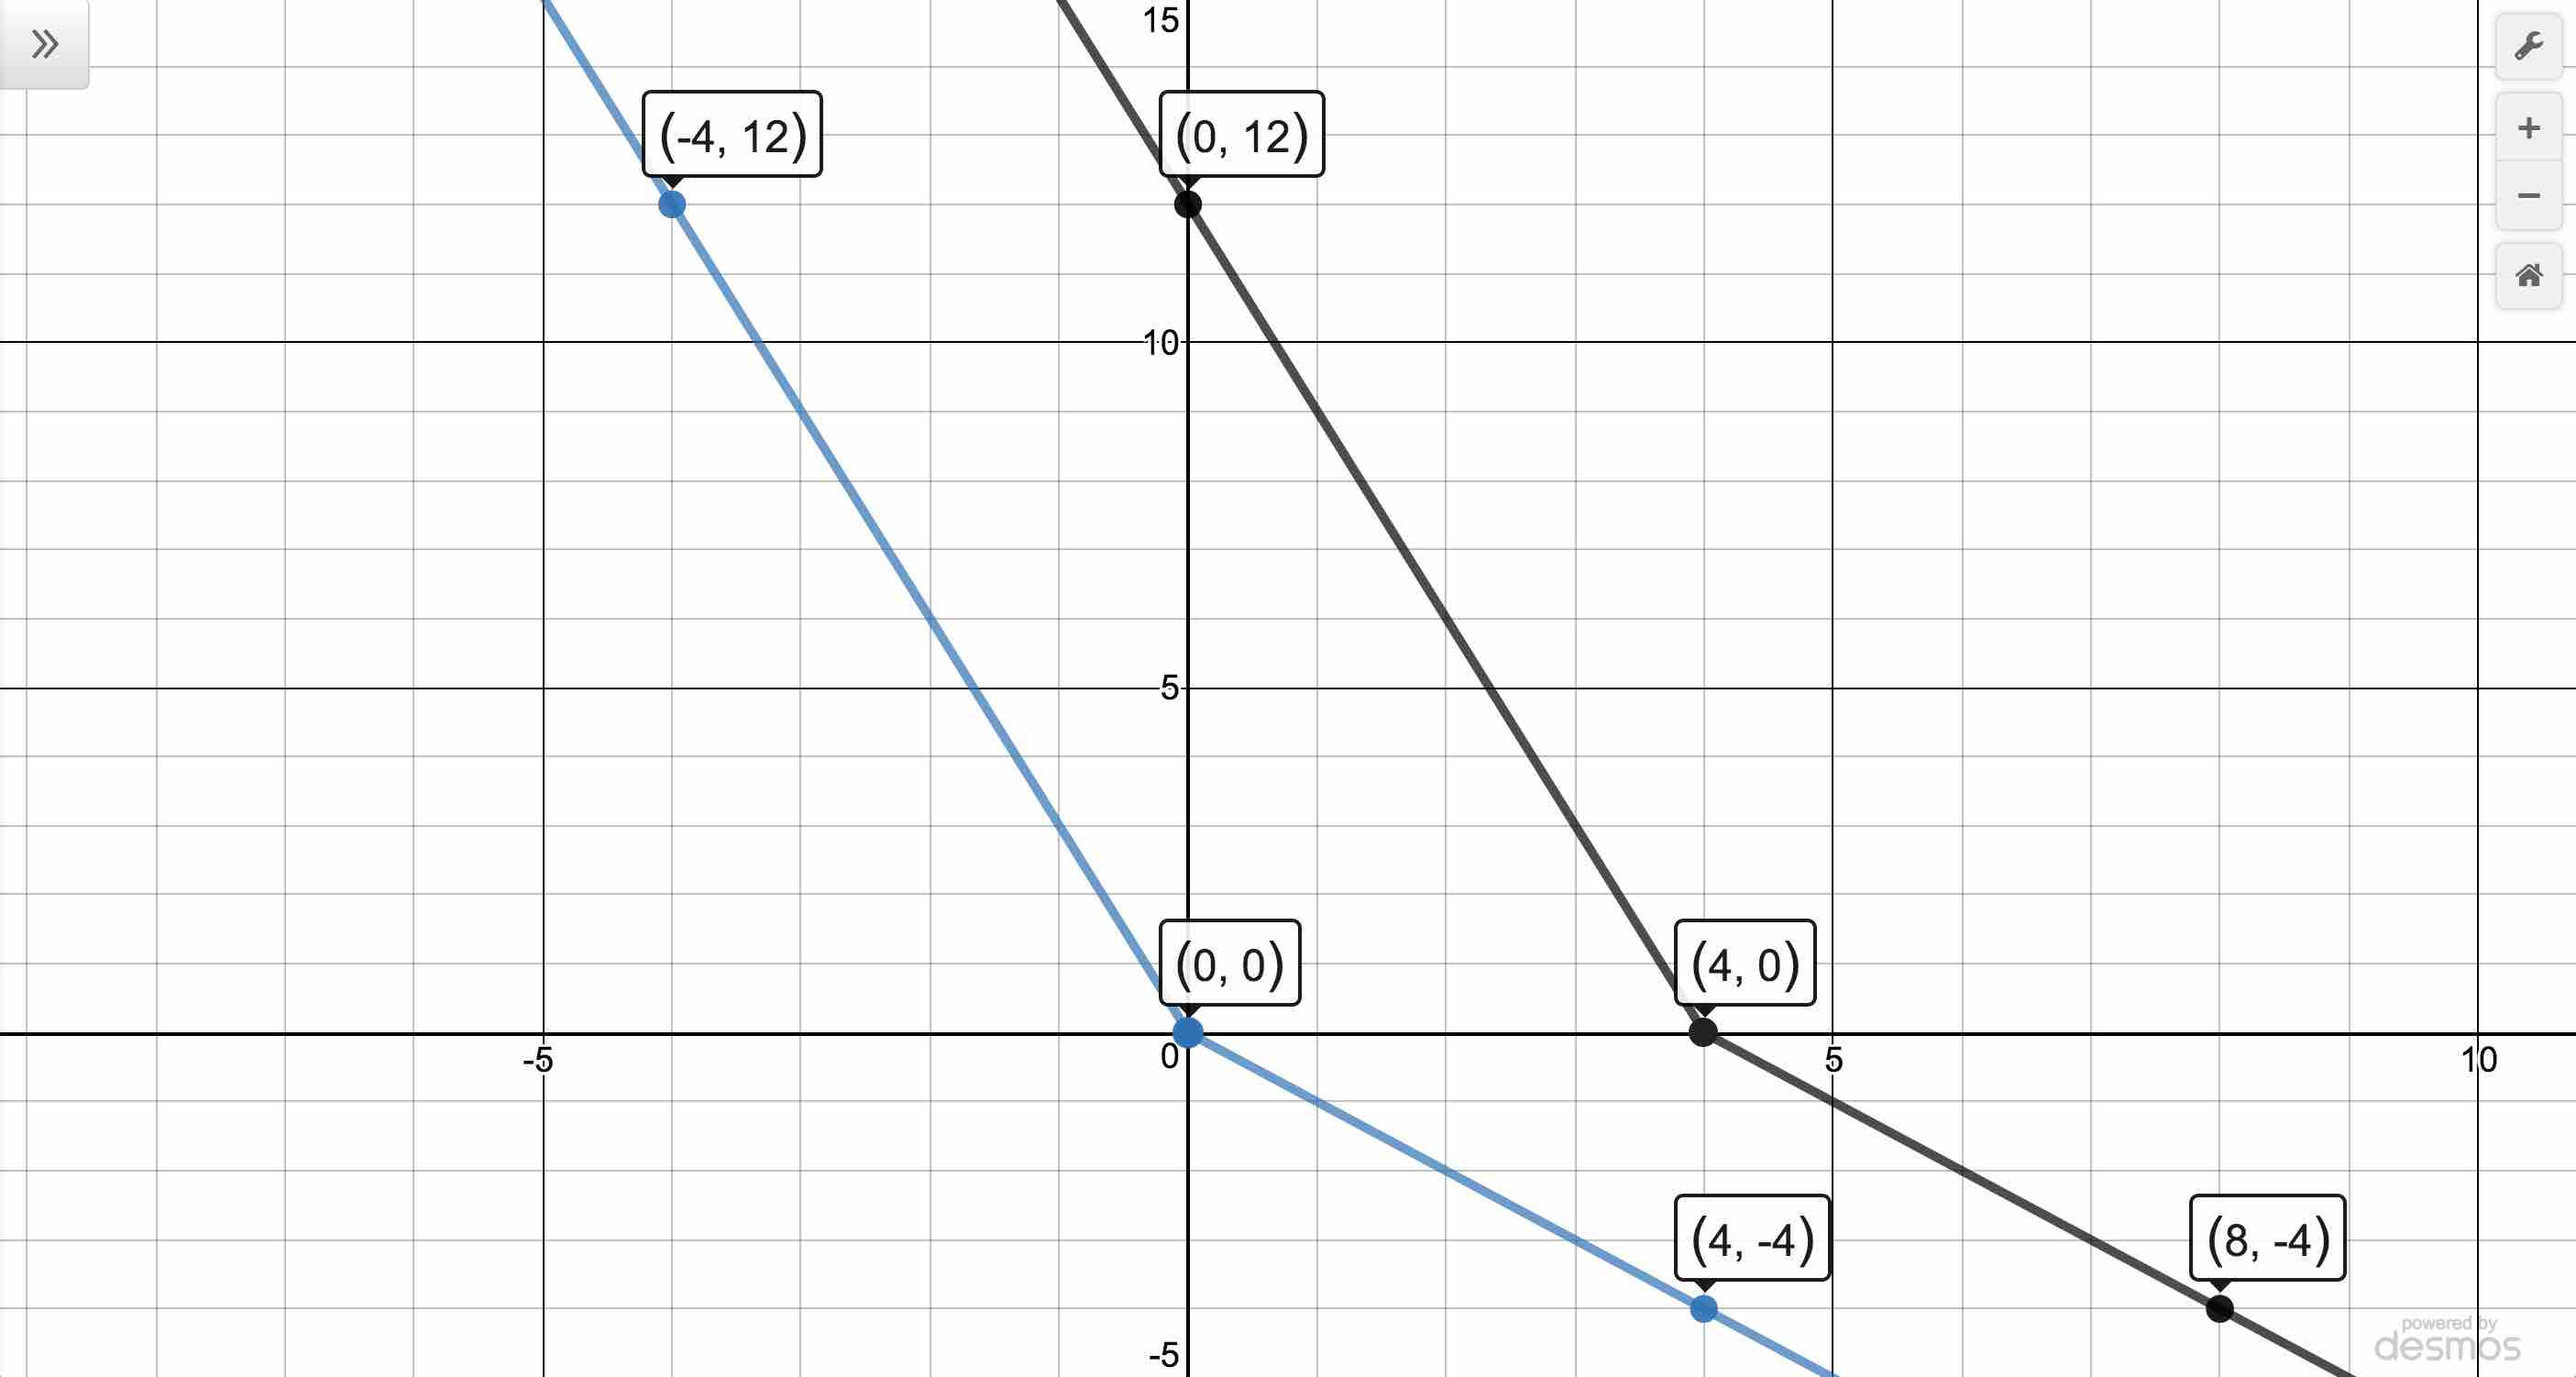
\includegraphics[width=3in]{./TransformationsGraphics/TransformationsEx01a.jpg} & 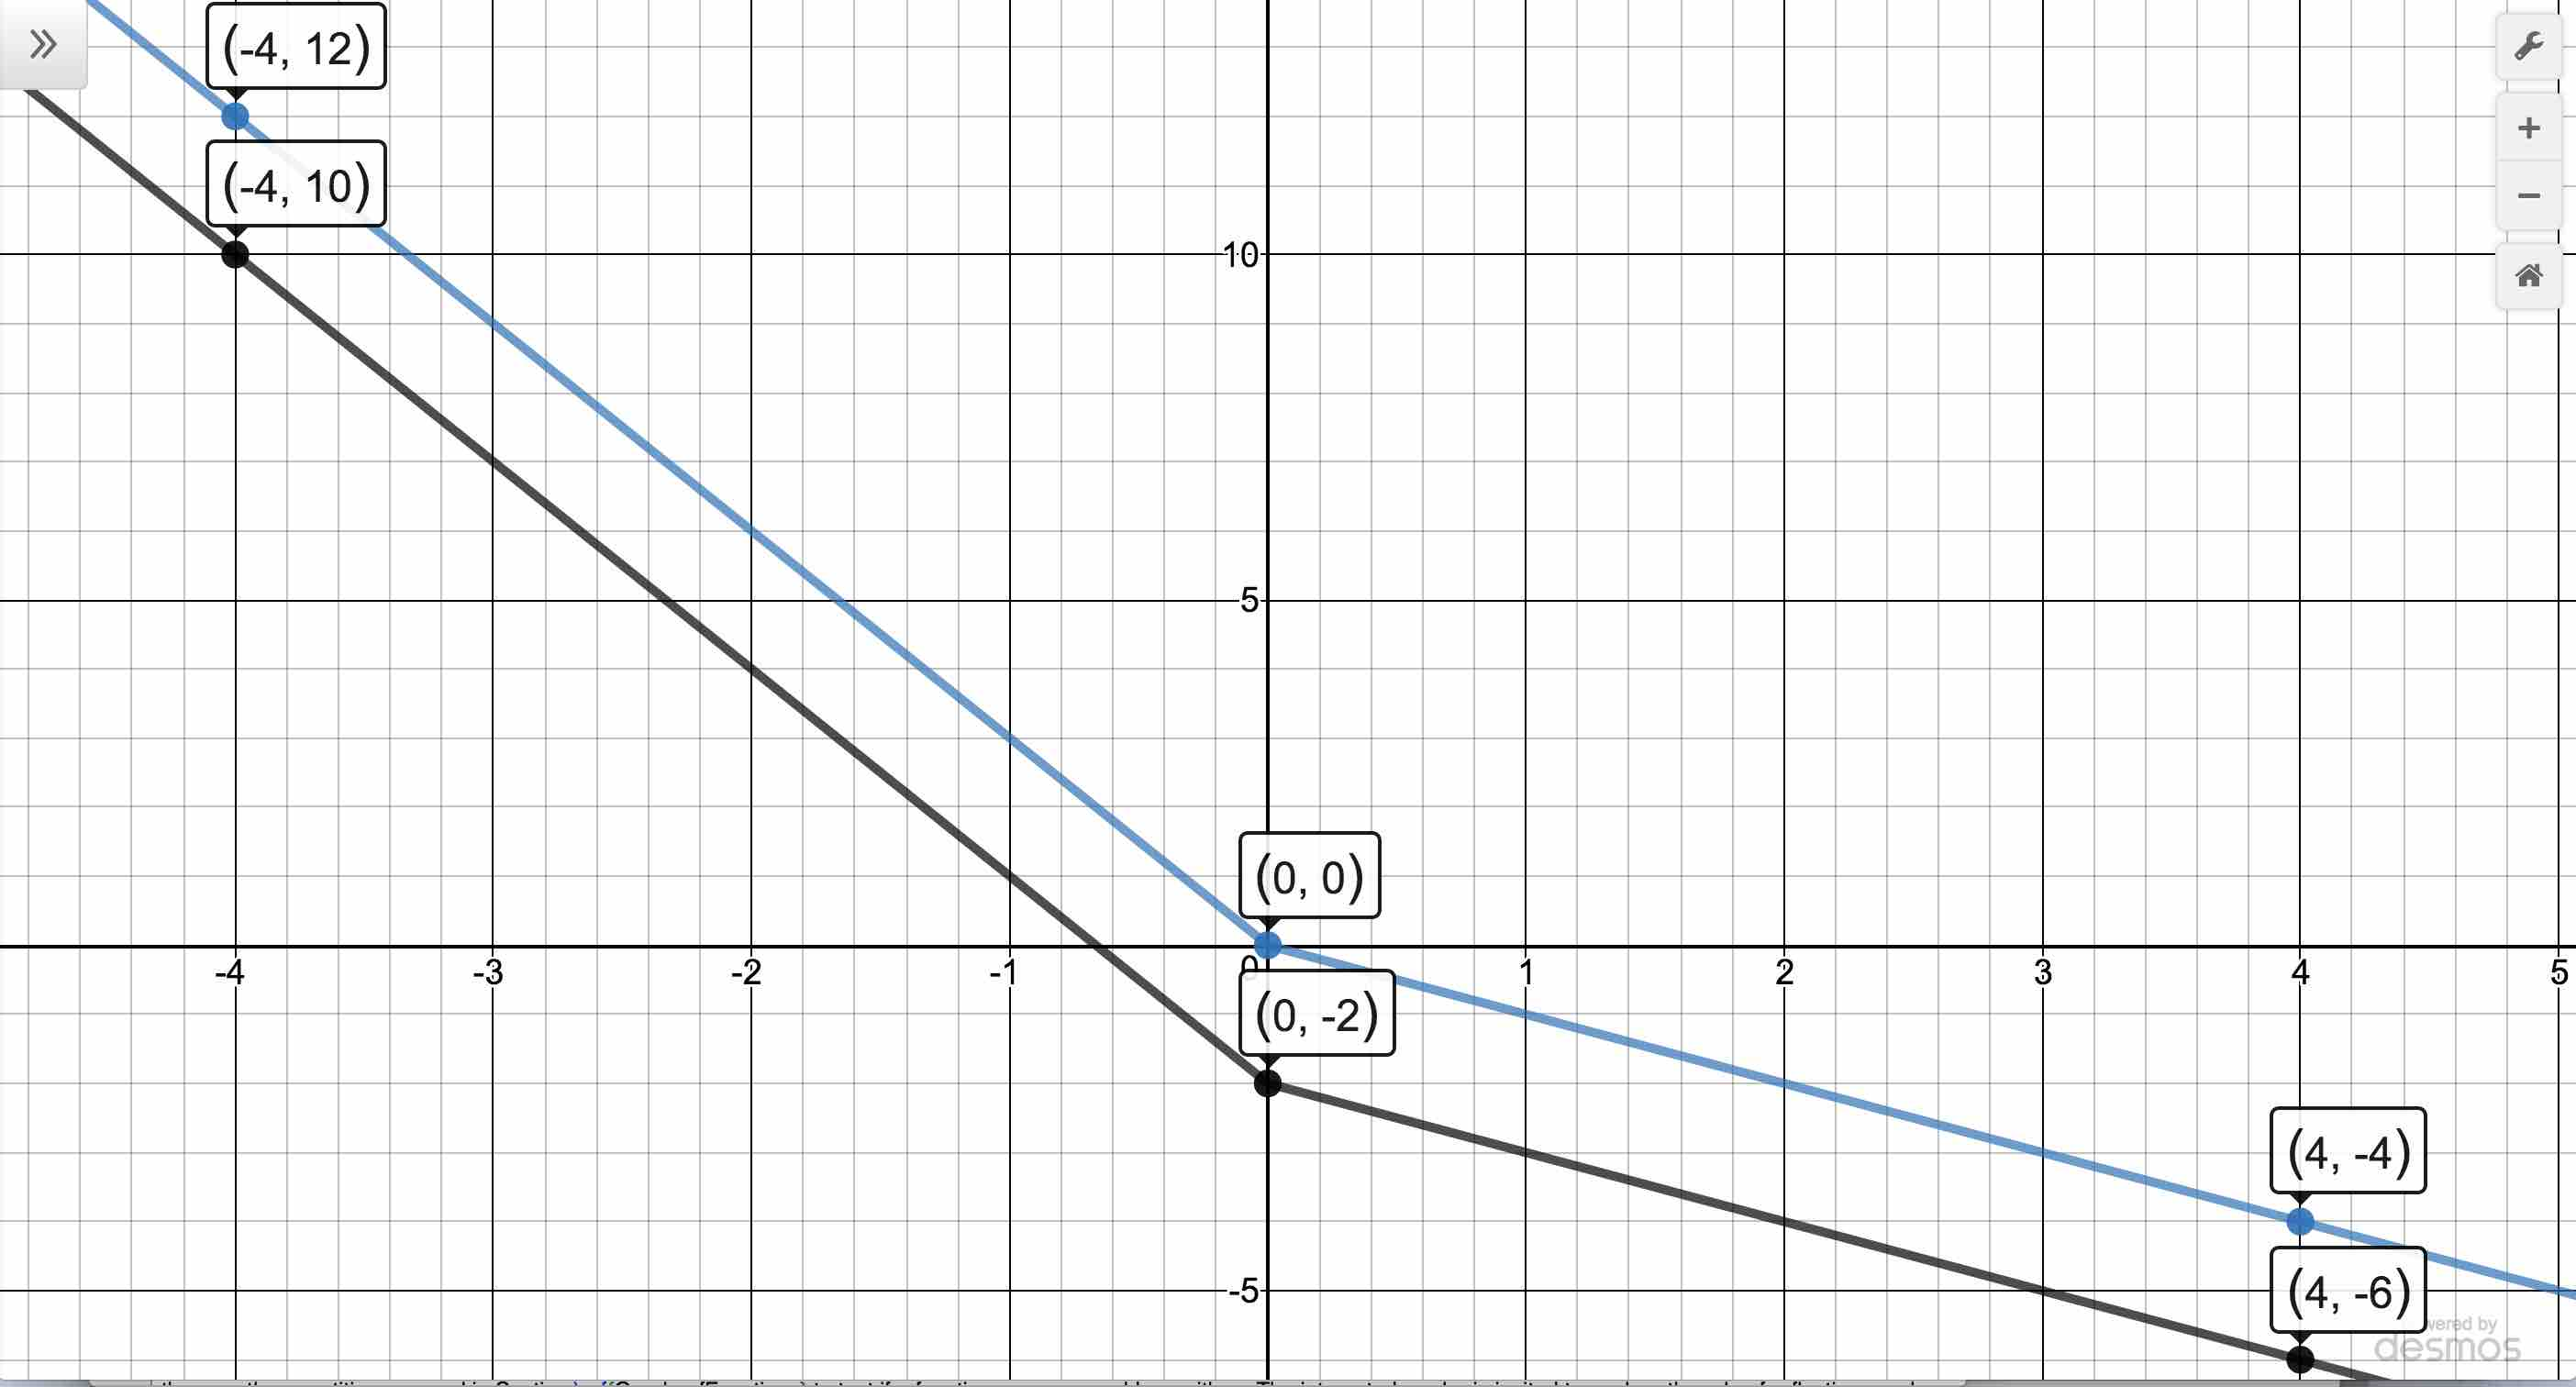
\includegraphics[width=3in]{./TransformationsGraphics/TransformationsEx01b.jpg} \\

$y =  |t|-2t$ (lighter color)  and $y = |t-4|-2t+8$  &  $y =  |t|-2t$ (lighter color) and $y =  |t|-2t-2$ \\

\end{tabular}

\end{center} 

\item  Comparing \textit{formulas}, it appears as if $F(x) = f(x-2)$.  We check: \[ f(x-2) = \dfrac{(x-2)^{\frac{2}{3}}}{(x-2)+2} = \dfrac{(x-2)^{\frac{2}{3}}}{x} = F(x),\]  so, per Theorem \ref{hshifts},  the graph of $y = F(x)$ should be the graph of $y=f(x)$ but shifted to the right $2$ units. We graph both functions below to confirm our answer.

\begin{center}

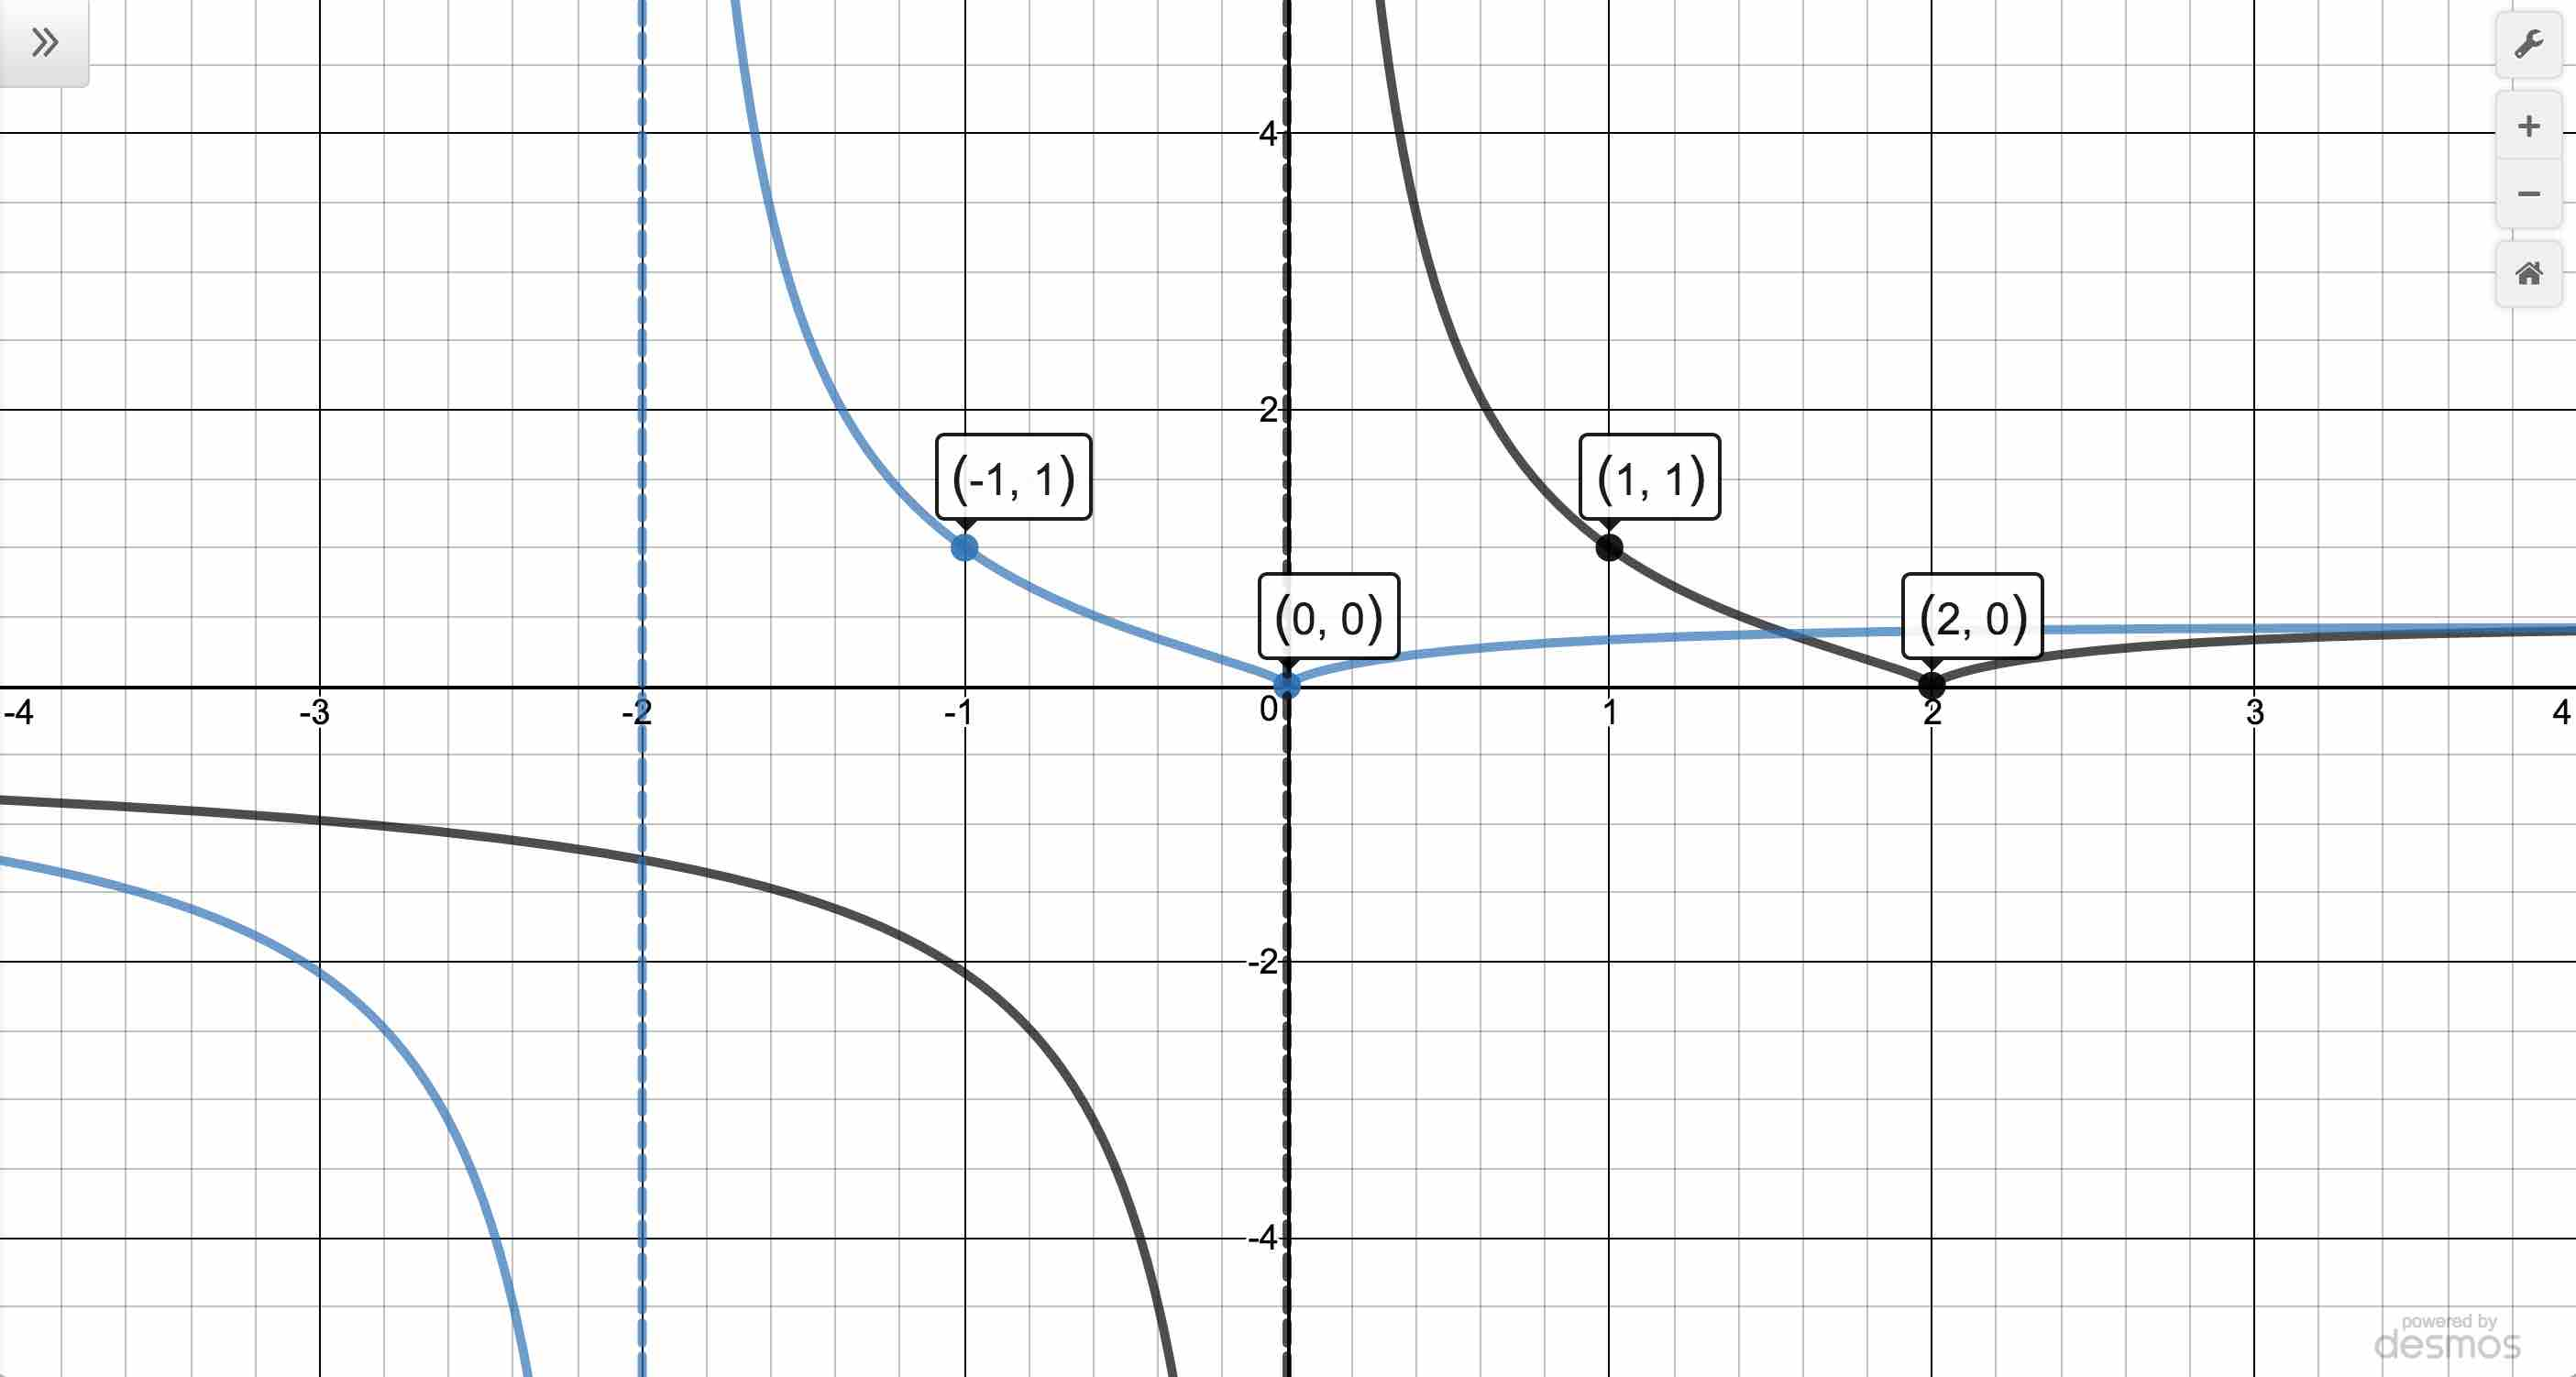
\includegraphics[width=4in]{./TransformationsGraphics/TransformationsEx01c.jpg}

$y = \dfrac{x^{\frac{2}{3}}}{x+2}$ (lighter color) and $y = \dfrac{(x-2)^{\frac{2}{3}}}{x}$ 

\end{center}

\item 

\begin{enumerate}  

\item  We recognize  $F(x) = f(x-2) =f(x-h)$. With $h=2$, Theorem \ref{hshifts} tells us to add $2$ to each of the $x$-coordinates of the points on the graph of $f$, moving the graph of $f$ to the \textit{right} two units.

\[\begin{array}{ccc}

\begin{mfpic}[15]{-3}{8}{-1}{5}
\axes
\tlabel[cc](8,-0.5){\scriptsize $x$}
\tlabel[cc](0.5,5){\scriptsize $y$}
\xmarks{-2, -1, 0, 1, 2, 3, 4,5,6,7}
\ymarks{0, 1, 2, 3,4}
\tcaption{\scriptsize $y = f(x)$}
\tlpointsep{4pt}
\scriptsize
\tlabel[cc](-2.25, -0.5){$(-2,0)$}
\tlabel[cc](-1, 3){$(0,3)$}
\tlabel[cc](2, 4.5){$(2,4)$}
\tlabel[cc](4, 2.5){$(4,3)$}
\axislabels {x}{{$1$} 1, {$2$} 2,  {$3$} 3,{$4$} 4,{$5$} 5,{$6$} 6,{$7$} 7}
\axislabels {y}{{$2$} 2,{$1$} 1,{$4$} 4}
\normalsize
\penwd{1.25pt}
\function{-2, 4, 0.1}{(x+2)*(6-x)/4}
\point[4pt]{(-2,0), (2,4), (0,3)}
\pointfillfalse
\point[4pt]{(4,3)}
\end{mfpic}

&

\stackrel{\stackrel{\mbox{\scriptsize shift right  $2$ units}}{\xrightarrow{\hspace{1in}}}}{\mbox{ \scriptsize add $2$ to each $x$-coordinate}} 

& 

\begin{mfpic}[15]{-3}{8}{-1}{5}
\axes
\tlabel[cc](8,-0.5){\scriptsize $x$}
\tlabel[cc](0.5,5){\scriptsize $y$}
\xmarks{-2, -1, 0, 1, 2, 3, 4,5,6,7}
\ymarks{0, 1, 2, 3,4}
\tcaption{\scriptsize $y = F(x) = f(x-2)$}
\tlpointsep{4pt}
\scriptsize
\gclear \tlabelrect(0, -0.5){$(0,0)$}
\tlabel[cc](1, 3){$(2,3)$}
\tlabel[cc](4, 4.5){$(4,4)$}
\tlabel[cc](6, 2.5){$(6,3)$}
\axislabels {x}{{$1$} 1, {$2$} 2,  {$3$} 3,{$4$} 4,{$5$} 5,{$6$} 6,{$7$} 7}
\axislabels {y}{{$2$} 2,{$1$} 1,{$4$} 4,{$3$} 3}
\normalsize
\penwd{1.25pt}
\function{0, 6, 0.1}{(x)*(8-x)/4}
\point[4pt]{(0,0), (4,4), (2,3)}
\pointfillfalse
\point[4pt]{(6,3)}
\end{mfpic}

\end{array}\]

We can check our answer by showing each ordered pair $(x,y)$ listed on our final graph satisfies the equation $y = f(x-2)$.  Starting with $(0,0)$, we substitute $x=0$ into $y=f(x-2)$ and get $y = f(0-2) = f(-2)$.  Since $(-2,0)$ is on the graph of $f$, we know $f(-2) = 0$.  Hence, $y = f(0-2) = f(-2) = 0$, showing the point $(0,0)$ is on the graph of $y=f(x-2)$.  We invite the reader to check the remaining points.

\item  We have $F(x) = f(x)+1 = f(x)+k$ where $k=1$, so  Theorem \ref{vshifts} tells us to move the graph of $f$ \textit{up} $1$ unit by adding $1$ to each of the $y$-coordinates of the points on the graph of $f$.

\[\begin{array}{ccc}

\begin{mfpic}[15]{-3}{6}{-1}{6}
\axes
\tlabel[cc](6,-0.5){\scriptsize $x$}
\tlabel[cc](0.5,6){\scriptsize $y$}
\xmarks{-2, -1, 0, 1, 2, 3, 4,5}
\ymarks{0, 1, 2, 3,4,5}
\tcaption{\scriptsize $y = f(x)$}
\tlpointsep{4pt}
\scriptsize
\tlabel[cc](-2.25, -0.5){$(-2,0)$}
\tlabel[cc](-1, 3){$(0,3)$}
\tlabel[cc](2, 4.5){$(2,4)$}
\tlabel[cc](4, 2.5){$(4,3)$}
\axislabels {x}{{$1$} 1, {$2$} 2,  {$3$} 3,{$4$} 4, {$5$} 5}
\axislabels {y}{{$2$} 2,{$1$} 1,{$4$} 4,{$5$} 5}
\normalsize
\penwd{1.25pt}
\function{-2, 4, 0.1}{(x+2)*(6-x)/4}
\point[4pt]{(-2,0), (2,4), (0,3)}
\pointfillfalse
\point[4pt]{(4,3)}
\end{mfpic}

&

\stackrel{\stackrel{\mbox{\scriptsize shift up $1$ unit}}{\xrightarrow{\hspace{1in}}}}{\mbox{ \scriptsize add $1$ to each $y$-coordinate}} 

& 

\begin{mfpic}[15]{-3}{6}{-1}{6}
\axes
\tlabel[cc](6,-0.5){\scriptsize $x$}
\tlabel[cc](0.5,6){\scriptsize $y$}
\xmarks{-2, -1, 0, 1, 2, 3, 4,5}
\ymarks{0, 1, 2, 3,4,5}
\tcaption{\scriptsize $y = F(x) =  f(x)+1$}
\tlpointsep{4pt}
\scriptsize
\tlabel[cc](-2.25, 0.5){$(-2,1)$}
\tlabel[cc](-1, 4){$(0,4)$}
\tlabel[cc](2, 5.5){$(2,5)$}
\tlabel[cc](4, 3.5){$(4,4)$}
\axislabels {x}{{$1$} 1, {$2$} 2,  {$3$} 3,{$4$} 4, {$5$} 5}
\axislabels {y}{{$2$} 2,{$1$} 1,{$3$} 3,{$5$} 5}
\normalsize
\penwd{1.25pt}
\function{-2, 4, 0.1}{1+(x+2)*(6-x)/4}
\point[4pt]{(-2,1), (2,5), (0,4)}
\pointfillfalse
\point[4pt]{(4,4)}
\end{mfpic}

\end{array}\]

To check our answer, we proceed as above.  Starting with the point $(-2,1)$, we substitute  $x=-2$ into $y=f(-2)+1$ to get $y = f(-2)+1$.  Since $(-2,0)$ is on the graph of $f$, we know $f(-2) = 0$.  Hence, $y = f(-2)+1 =0+1 = 1$.  This proves $(-2,1)$ is on the graph of $y=f(x)+1$.  We encourage the reader to check the remaining points in kind. 

\item  We are asked to graph $F(x) = f(x+1) -2$.  As above, when we have more than one modification to do, we work from the inside out and build up to $F(x)=f(x+1)-2$  from $f(x)$ in stages.   First, we apply Theorem \ref{hshifts} to graph $y=f(x+1)$ from $y=f(x)$.   Rewriting $f(x+1) = f(x-(-1))$, we identify $h=-1$,  so we add  $-1$ to (subtract $1$ from) each of the $x$-coordinates on the graph of $f$, shifting it to the \textit{left} $1$ unit.

\[\begin{array}{ccc}

\begin{mfpic}[15]{-4}{6}{-1}{5}
\axes
\tlabel[cc](6,-0.5){\scriptsize $x$}
\tlabel[cc](0.5,5){\scriptsize $y$}
\xmarks{-3,-2, -1, 0, 1, 2, 3, 4,5}
\ymarks{0, 1, 2, 3,4}
\tcaption{\scriptsize $y = f(x)$}
\tlpointsep{4pt}
\scriptsize
\tlabel[cc](-2.25, -0.5){$(-2,0)$}
\tlabel[cc](-1, 3){$(0,3)$}
\tlabel[cc](2, 4.5){$(2,4)$}
\tlabel[cc](4, 2.5){$(4,3)$}
\axislabels {x}{{$1$} 1, {$2$} 2,  {$3$} 3,{$4$} 4, {$5$} 5}
\axislabels {y}{{$2$} 2,{$1$} 1,{$4$} 4}
\normalsize
\penwd{1.25pt}
\function{-2, 4, 0.1}{(x+2)*(6-x)/4}
\point[4pt]{(-2,0), (2,4), (0,3)}
\pointfillfalse
\point[4pt]{(4,3)}
\end{mfpic}

&

\stackrel{\stackrel{\mbox{\scriptsize shift left $1$ unit}}{\xrightarrow{\hspace{1in}}}}{\mbox{ \scriptsize subtract $1$ from each $x$-coordinate}} 

& 

\begin{mfpic}[15]{-4}{6}{-1}{5}
\axes
\tlabel[cc](6,-0.5){\scriptsize $x$}
\tlabel[cc](0.5,5){\scriptsize $y$}
\xmarks{-3,-2, -1, 0, 1, 2, 3, 4,5}
\ymarks{0, 1, 2, 3,4}
\tcaption{\scriptsize $y  = f(x+1)$}
\tlpointsep{4pt}
\scriptsize
\tlabel[cc](-3.25, -0.5){$(-3,0)$}
\tlabel[cc](-2, 3){$(1,3)$}
\tlabel[cc](1, 4.5){$(1,4)$}
\tlabel[cc](3, 2.5){$(3,3)$}
\axislabels {x}{{$1$} 1, {$2$} 2,  {$3$} 3,{$4$} 4, {$5$} 5, {\scriptsize $-1\hspace{7pt}$} -1}
\axislabels {y}{{$2$} 2,{$1$} 1,{$4$} 4}
\normalsize
\penwd{1.25pt}
\function{-3, 3, 0.1}{(x+3)*(5-x)/4}
\point[4pt]{(-3,0), (1,4), (-1,3)}
\pointfillfalse
\point[4pt]{(3,3)}
\end{mfpic}

\end{array}\]

Next, we apply Theorem \ref{vshifts}  to graph $y = f(x+1)-2$ starting with the graph of $y=f(x+1)$.  Writing $f(x+1)-2=f(x+1)+(-2) = f(x+1)+k$, we identify $k=-2$ so  Theorem \ref{vshifts} instructs us to add $-2$ to (subtract $2$ from) each of the $y$-coordinates on the graph of $y = f(x+1)$, thereby shifting the graph \textit{down} two units.

\[\begin{array}{ccc}

\begin{mfpic}[15]{-4}{6}{-3}{5}
\axes
\tlabel[cc](6,-0.5){\scriptsize $x$}
\tlabel[cc](0.5,5){\scriptsize $y$}
\xmarks{-3,-2, -1, 0, 1, 2, 3, 4,5}
\ymarks{-2, -1, 0, 1, 2, 3,4}
\tcaption{\scriptsize $y = f(x+1)$}
\tlpointsep{4pt}
\scriptsize
\tlabel[cc](-3.25, -0.5){$(-3,0)$}
\tlabel[cc](-2, 3){$(1,3)$}
\tlabel[cc](1, 4.5){$(1,4)$}
\tlabel[cc](3, 2.5){$(3,1)$}
\axislabels {x}{{$1$} 1, {$2$} 2,  {$3$} 3,{$4$} 4, {$5$} 5, {\scriptsize $-1\hspace{7pt}$} -1}
\axislabels {y}{{$2$} 2,{$1$} 1,{$4$} 4,{$-1$} -1,{$-2$} -2, ,{$3$} 3}
\normalsize
\penwd{1.25pt}
\function{-3, 3, 0.1}{(x+3)*(5-x)/4}
\point[4pt]{(-3,0), (1,4), (-1,3)}
\pointfillfalse
\point[4pt]{(3,3)}
\end{mfpic}

&

\stackrel{\stackrel{\mbox{\scriptsize shift down $2$ units}}{\xrightarrow{\hspace{1in}}}}{\mbox{ \scriptsize subtract $2$ from each $y$-coordinate}} 

& 


\begin{mfpic}[15]{-4}{6}{-3}{5}
\axes
\tlabel[cc](6,-0.5){\scriptsize $x$}
\tlabel[cc](0.5,5){\scriptsize $y$}
\xmarks{-3,-2, -1, 0, 1, 2, 3, 4,5}
\ymarks{-2, -1, 0, 1, 2, 3,4}
\tcaption{\scriptsize $y = f(x+1)-2=F(x)$}
\tlpointsep{4pt}
\scriptsize
\tlabel[cc](-3.25, -2.5){$(-3,-2)$}
\tlabel[cc](-2, 1){$(1,1)$}
\tlabel[cc](1, 2.5){$(1,2)$}
\tlabel[cc](3, 0.5){$(3,2)$}
\axislabels {x}{{$1$} 1, {$2$} 2,  {$3$} 3,{$4$} 4, {$5$} 5, {\scriptsize $-1\hspace{7pt}$} -1}
\axislabels {y}{{$2$} 2,{$1$} 1,{$4$} 4,{$-1$} -1,{$-2$} -2, ,{$3$} 3}
\normalsize
\penwd{1.25pt}
\function{-3, 3, 0.1}{((x+3)*(5-x)/4)-2}
\point[4pt]{(-3,-2), (1,2), (-1,1)}
\pointfillfalse
\point[4pt]{(3,1)}
\end{mfpic}

\end{array}\]

To check, we start with the point $(-3, -2)$.  We find when we substitute $x=-3$ into the equation $y=f(x+1)-2$ we get $y = f(-3+1)-2 = f(-2)-2$.  Since $(-2,0)$ is on the graph of $f$, we know $f(-2) =0$, so  $y = f(-3+1)-2 = f(-2)-2 = 0 - 2 = -2$.  This proves $(-3,-2)$ is on the graph of $y=f(x+1)-2$.  We leave the checks of the remaining points to the reader.

\end{enumerate}

\item  To write $g(x)$ in terms of $f(x)$, we note that based on points which are labeled, it appears as if the graph of $g$ can be obtained from the graph of $f$ by shifting the graph of $f$ to the right $0.5$ units and down $1$ unit.  

\smallskip

Per Theorems \ref{hshifts} and \ref{vshifts}, $g(x)$ must take the form $g(x) = f(x-h)+k$.  Since the horizontal shift is to the \textit{right} $0.5$ units, $h = 0.5$ and since the vertical shift is \textit{down} $1$ unit, $k = -1$.   Hence, we get $g(x) = f(x-0.5)-1$.  

\smallskip

We can check our answer by working through both transformations, in sequence, as in the previous example.   To write $f(x)$ in terms of $g(x)$, we need to reverse the process - that is, we need to shift the graph of $g$ \textit{left} one half of a unit and \textit{up} one unit.   Theorems \ref{hshifts} and \ref{vshifts} suggest the formula $f(x) = g(x+0.5)+1$.  We leave it to the reader to check. \qed
  
 \end{enumerate}
 
 \end{ex}
 
\subsection{Reflections about the Coordinate Axes}

We now turn our attention to reflections. We know from Section \ref{AppCartesianPlane} that to reflect a point $(x,y)$ across the $x$-axis, we replace $y$ with $-y$.  If $(x,y)$ is on the graph of $f$, then $y=f(x)$, so replacing $y$ with $-y$ is the same as replacing $f(x)$ with $-f(x)$.  Hence, the graph of $y=-f(x)$ is the graph of $f$ reflected across the $x$-axis.  Similarly, the graph of $y=f(-x)$ is the graph of $y = f(x)$ reflected across the $y$-axis.\footnote{The expressions $-f(x)$ and $f(-x)$ should look familiar - they are the quantities we used in Section \ref{GraphsofPolynomials} to determine if a function was even, odd or neither.  We explore impact of symmetry on reflections in Exercise \ref{SymmetryandReflectionsExercise}.}   

\smallskip

\colorbox{ResultColor}{\bbm

%\smallskip

\begin{thm} \label{reflections}\index{graph ! reflection about an axis}\index{reflection ! of a function graph}\textbf{Reflections.}  Suppose $f$ is a function. 

  To graph $F(x)=-f(x)$,  multiply each of the $y$-coordinates of the points on the graph of $y=f(x)$ by $-1$.

\textbf{NOTE:}  This results in a reflection across the $x$-axis.

To graph $F(x)=f(-x)$,  multiply each of the $x$-coordinates of the points on the graph of $y=f(x)$ by $-1$.

\textbf{NOTE:}  This results in a reflection across the $y$-axis.


\end{thm}

\ebm}

\smallskip

The proof of Theorem \ref{reflections} follows in much the same way as the proofs of Theorems \ref{vshifts} and \ref{hshifts}.  If $c$ is an element of the domain of $f$ and $F(x) = -f(x)$,  then the point $(c, f(c))$ corresponds to the point $(c, F(c)) = (c,-f(c))$.  Comparing the corresponding points $(c, f(c))$ and $(c, -f(c))$, we see they only difference is the $y$-coordinates are the exact opposite - indicating they are mirror-images across the $x$-axis.  Similarly, if $c$ is an element in the domain of $f$, then $c$ corresponds to the element $-c$ in the domain of $F(x) = f(-x)$ since $F(-c) = f(-(-c)) = f(c)$. Hence, the corresponding points here are $(c, f(c))$ and $(-c, F(-c)) = (-c, f(c))$.  Comparing $(c, f(c))$ with $(-c, f(c))$, we see they are reflections about the $y$-axis.

\smallskip

Using the  language of inputs and outputs, Theorem \ref{reflections} says that multiplying the \textit{outputs} from a function by $-1$ reflects its graph across the \textit{horizontal} axis, while multiplying the \textit{inputs} to a function by $-1$ reflects the graph across the \textit{vertical} axis.

\smallskip

Applying Theorem \ref{reflections} to the graph of $y=f(x)$ given at the beginning of the section, we can graph $y=-f(x)$ by reflecting the graph of $f$ about the $x$-axis.

\[ \begin{array}{|c||c|c|c|c|}  

\hline

 x & (x,f(x)) & f(x) & g(x)=-f(x) & (x, g(x)) \\ \hline
0  & (0,1)& 1 & -1 &(0, -1) \\  \hline
2 & (2,3) & 3 &  -3 &(2,-3) \\  \hline
4 & (4,3) & 3 &  -3&(4, -3) \\  \hline
5 & (5,5) & 5 &  -5 &( 5 ,-5) \\  \hline

\end{array} \] 

\[ \begin{array}{ccc}

\begin{mfpic}[14]{-1}{6}{-6}{6}
\tlabel[cc](-1,1){\scriptsize $(0,1)$}
\tlabel[cc](2,3.5){\scriptsize $(2,3)$}
\tlabel[cc](4,2.5){\scriptsize $(4,3)$}
\tlabel[cc](5,5.5){\scriptsize $(5,5)$}
\tlabel[cc](6,-0.5){\scriptsize $x$}
\tlabel[cc](0.5,6){\scriptsize $y$}
\tcaption{\scriptsize $y=f(x)$}
\axes
\xmarks{1,2,3,4,5}
\ymarks{-1,-2,-3,-4,-5,1,2,3,4,5}
\tlpointsep{4pt}
\axislabels {x}{{\scriptsize $1$} 1, {\scriptsize $2$} 2, {\scriptsize $3$} 3, {\scriptsize $4$} 4, {\scriptsize $5$} 5}
\axislabels {y}{{\scriptsize $-1$} -1,{\scriptsize $-2$} -2, {\scriptsize $-3$} -3, {\scriptsize $-4$} -4, {\scriptsize $-5$} -5, {\scriptsize $2$} 2, {\scriptsize $3$} 3, {\scriptsize $4$} 4, {\scriptsize $5$} 5}
\penwd{1.25pt}
\polyline{(0,1), (2,3), (4,3), (5,5)}
\point[4pt]{(0,1), (2,3), (4,3), (5,5)}
\end{mfpic}

&

\stackrel{\stackrel{\mbox{\scriptsize reflect across $x$-axis}}{\xrightarrow{\hspace{1in}}}}{\mbox{ \scriptsize multiply each $y$-coordinate by $-1$}} 

&

\begin{mfpic}[14]{-1}{6}{-6}{6}
\tlabel[cc](-1.25,-1){\scriptsize $(0,-1)$}
\tlabel[cc](2,-3.5){\scriptsize $(2,-3)$}
\tlabel[cc](4,-2.5){\scriptsize $(4,-3)$}
\tlabel[cc](5,-5.5){\scriptsize $(5,-5)$}
\tlabel[cc](6,-0.5){\scriptsize $x$}
\tlabel[cc](0.5,6){\scriptsize $y$}
\tcaption{\scriptsize $y=-f(x)$}
\axes
\xmarks{1,2,3,4,5}
\ymarks{-1,-2,-3,-4,-5,1,2,3,4,5}
\tlpointsep{4pt}
\axislabels {x}{{\scriptsize $1$} 1, {\scriptsize $2$} 2, {\scriptsize $3$} 3, {\scriptsize $4$} 4, {\scriptsize $5$} 5}
\axislabels {y}{{\scriptsize $-2$} -2, {\scriptsize $-3$} -3, {\scriptsize $-4$} -4, {\scriptsize $-5$} -5,{\scriptsize $1$} 1,{\scriptsize $2$} 2, {\scriptsize $3$} 3, {\scriptsize $4$} 4, {\scriptsize $5$} 5}
\penwd{1.25pt}
\polyline{(0,-1), (2,-3), (4,-3), (5,-5)}
\point[4pt]{(0,-1), (2,-3), (4,-3), (5,-5)}
\end{mfpic}

\end{array}\]

By reflecting the graph of $f$ across the $y$-axis, we obtain the graph of $y=f(-x)$.

\[ \begin{array}{|r||c|c|c|}  

\hline

x & -x & g(x)=f(-x) & (x, g(x)) \\ \hline
0 & 0 & g(0)=f(-(-0)) = f(0) = 1   &(0, 1) \\  \hline
-2 & 2 &  g(-2)=f(-(-2)) = f(2) = 3  &(-2,3) \\  \hline
-4 & 4 & g(-4)=f(-(-4)) = f(4) = 3 &  (-4,3)\\  \hline
-5 & 5 & g(-5)=f(-(-5)) = f(5) = 5  & (-5,5) \\  \hline

\end{array} \]

\[ \begin{array}{ccc}

\begin{mfpic}[13]{-6}{6}{-1}{6}
\tlabel[cc](-1,1){\scriptsize $(0,1)$}
\tlabel[cc](2,3.5){\scriptsize $(2,3)$}
\tlabel[cc](4,2.5){\scriptsize $(4,3)$}
\tlabel[cc](5,5.5){\scriptsize $(5,5)$}
\tlabel[cc](6,-0.5){\scriptsize $x$}
\tlabel[cc](0.5,6){\scriptsize $y$}
\tcaption{\scriptsize $y=f(x)$}
\axes
\xmarks{-1,-2,-3,-4,-5,1,2,3,4,5}
\ymarks{1,2,3,4,5}
\tlpointsep{4pt}
\axislabels {x}{{\scriptsize $-1 \hspace{7pt}$} -1, {\scriptsize $-2\hspace{7pt}$} -2, {\scriptsize $-3\hspace{7pt}$} -3, {\scriptsize $-4\hspace{7pt}$} -4, {\scriptsize $-5\hspace{7pt}$} -5, {\scriptsize $1$} 1, {\scriptsize $2$} 2, {\scriptsize $3$} 3, {\scriptsize $4$} 4, {\scriptsize $5$} 5}
\axislabels {y}{{\scriptsize $2$} 2, {\scriptsize $3$} 3, {\scriptsize $4$} 4, {\scriptsize $5$} 5}
\penwd{1.25pt}
\polyline{(0,1), (2,3), (4,3), (5,5)}
\point[4pt]{(0,1), (2,3), (4,3), (5,5)}
\end{mfpic}

&

\stackrel{\stackrel{\mbox{\scriptsize reflect across $y$-axis}}{\xrightarrow{\hspace{1in}}}}{\mbox{ \scriptsize multiply each $x$-coordinate by $-1$}} 

&

\begin{mfpic}[13]{-6}{6}{-1}{6}
\tlabel[cc](1,1){\scriptsize $(0,1)$}
\tlabel[cc](-2,3.5){\scriptsize $(-2,3)$}
\tlabel[cc](-4,2.5){\scriptsize $(-4,3)$}
\tlabel[cc](-5,5.5){\scriptsize $(-5,5)$}
\tlabel[cc](6,-0.5){\scriptsize $x$}
\tlabel[cc](0.5,6){\scriptsize $y$}
\tcaption{\scriptsize $y=f(-x)$}
\axes
\xmarks{-1,-2,-3,-4,-5,1,2,3,4,5}
\ymarks{1,2,3,4,5}
\tlpointsep{4pt}
\axislabels {x}{{\scriptsize $-1 \hspace{7pt}$} -1, {\scriptsize $-2\hspace{7pt}$} -2, {\scriptsize $-3\hspace{7pt}$} -3, {\scriptsize $-4\hspace{7pt}$} -4, {\scriptsize $-5\hspace{7pt}$} -5, {\scriptsize $1$} 1, {\scriptsize $2$} 2, {\scriptsize $3$} 3, {\scriptsize $4$} 4, {\scriptsize $5$} 5}
\axislabels {y}{{\scriptsize $2$} 2, {\scriptsize $3$} 3, {\scriptsize $4$} 4, {\scriptsize $5$} 5}
\penwd{1.25pt}
\polyline{(0,1), (-2,3), (-4,3), (-5,5)}
\point[4pt]{(0,1), (-2,3), (-4,3), (-5,5)}
\end{mfpic}

\end{array}\]

\begin{ex}  \label{reflectionsex}  

Use Theorems  \ref{vshifts},  \ref{hshifts} and \ref{reflections}  to answer the questions below.  Check your answers using a graphing utility where appropriate.
 
 \begin{enumerate}
 
 \item   Suppose $(2,-5)$ is on the graph of $y = f(x)$.  Find a point on the graph of:
 
 \begin{multicols}{3}
 
 \begin{enumerate}
 
 \item $y = f(-x)$
 
 \item $y = -f(x+2)$
 
 \item  \label{twotransxrefex} $f(8-x)$
 
 \end{enumerate}
 
 \end{multicols}
 
 \item  Find a formula for a function $H(s)$ whose graph is the same as $t=h(s) = s^3-s^2$ but is reflected across the $t$-axis.
 
 \item Predict how the graph of $G(t) = \dfrac{t+4}{t-3}$ relates to the graph of $g(t) =\dfrac{t+4}{3-t}$ . 
 
\item  Below on the left is the graph of $y = f(x)$.  Use it to sketch the graph of

  \begin{multicols}{2}
 
 \begin{enumerate}
 
 \item $F(x) = f(-x)+1$
 
  \item \label{twotransyrefex}  $F(x)= 1 - f(2-x)$
 
 \end{enumerate}
 
 \end{multicols}
 
 \item \label{gfromfrefex} Below on the right is the graph of $y = g(x)$.  Write $g(x)$ in terms of $f(x)$ and vice-versa.
 
\begin{center}

\begin{multicols}{2}

\begin{mfpic}[15]{-3}{3}{-1}{6}
\axes
\tlabel[cc](3,-0.5){\scriptsize $x$}
\tlabel[cc](0.5,6){\scriptsize $y$}
\xmarks{-2, -1, 0, 1, 2}
\ymarks{ 0, 1, 2, 3,4,5}
\tcaption{\scriptsize $y = f(x)$}
\tlpointsep{4pt}
\scriptsize
\tlabel[cc](1, 1){$(0,1)$}
\tlabel[cc](2, 2){$(1,2)$}
\tlabel[cc](2.75, 4){$(2,4)$}
\axislabels {x}{{\scriptsize $-2 \hspace{7pt}$} -2,{\scriptsize $-1 \hspace{7pt}$} -1,{$1$} 1, {$2$} 2}
\axislabels {y}{{$2$} 2,{$3$} 3,{$4$} 4,{$5$} 5}
\normalsize
\penwd{1.25pt}
\arrow \reverse \arrow \function{-2.5, 2.5, 0.1}{2**x}
\point[4pt]{(0,1), (1,2), (2,4)}
\end{mfpic}



\begin{mfpic}[15]{-4}{2}{-2}{5}
\axes
\tlabel[cc](2,-0.5){\scriptsize $x$}
\tlabel[cc](0.5,5){\scriptsize $y$}
\xmarks{-2, -1, 0, 1}
\ymarks{ -1, 0, 1, 2, 3,4}
\tcaption{\scriptsize $y = g(x)$}
\tlpointsep{4pt}
\scriptsize
\tlabel[cc](-2, 2.5){$(-1,3)$}
\tlabel[cc](1, 2){$(0,2)$}
\tlabel[cc](1.5, 0.5){$(1,0)$}
\axislabels {x}{{\scriptsize $-3 \hspace{7pt}$} -3,{\scriptsize $-2 \hspace{7pt}$} -2,{\scriptsize $-1 \hspace{7pt}$} -1}
\axislabels {y}{{$-1$} -1,{$1$} 1,{$2$} 2,{$3$} 3,{$4$} 4}
\normalsize
\dashed \polyline{(-4,4), (2,4)}
\penwd{1.25pt}
\arrow \reverse \arrow \function{-3.5, 1.5, 0.1}{4-(2**(x+1))}
\point[4pt]{(-1,3), (0,2), (1,0)}
\end{mfpic}
 
\end{multicols}

\text{\scriptsize \textbf{NOTE:}  The $x$-axis, $y=0$, is a horizontal asymptote to the graph of $y = f(x)$ and the line $y=4$ is a horizontal asymptote to the graph of $y = g(x)$. }
\end{center}
 
 \end{enumerate}
 
 \newpage
 
 {\bf Solution.}
 
 \begin{enumerate}
 
 \item 
 
 \begin{enumerate}
 
 \item To find a point on the graph of $y=f(-x)$, Theorem \ref{reflections} tells us to multiply the $x$-coordinate of the point on the graph of $y=f(x)$ by $-1$:  $((-1)2, -5) = (-2,-5)$.  
 
 \smallskip
 
 To check, since $(2,-5)$ is on the graph of $f$, we know $f(2) = -5$.  Hence, when we substitute $x=-2$ into $y = f(-x)$, we get $y = f(-(-2)) = f(2) = -5$, proving $(-2,-5)$ is on the graph of $y=f(-x)$.
 
 \item To find a point on the graph of $y = -f(x+2)$, we first note we have two transformations at work here, so we work our way from the inside out and build $f(x)$ to $-f(x+2)$. 
 
 \smallskip
 
 First, we find a point on the graph of $y=f(x+2)$.  Writing $f(x+2) = f(x-(-2))$, we apply Theorem \ref{hshifts} with $h=-2$ and add $-2$ to (or subtract $2$ from) the $x$-coordinate of the point we know is on $y=f(x)$:   $(2-2,-5) =  (0,-5)$. 
 
 \smallskip
 
  Next we apply Theorem \ref{reflections} to the graph of $y=f(x+2)$ to get a point on the graph of $y=-f(x+2)$ by multiplying the $y$-coordinate of $(0,-5)$ by $-1$:  $(0, (-1)(-5)) = (0,5)$.  
  
  \smallskip
  
  To check, recall $f(2)=-5$ so that when we substitute $x=0$ into the equation $y = -f(x+2)$, we get $y=-f(0+2) = -f(2) = -(-5)=5$, as required. 
 
 
 \item  Rewriting  $f(8-x) = f(-x+8)$ we see we have two transformations at play here:  a reflection across the $y$-axis and a horizontal shift.  Since both of these transformations affect the $x$-coordinates of the graph, the question becomes which transformation to address first. To help us with this decision, we attack the problem algebraically.  
 
 \smallskip
 
 Recall that since $(2,-5)$ is on the graph of $f$, we know  $f(2) = -5$.  Hence, to get a point on the graph of $y = f(-x+8)$, we need to match up the arguments of $f(-x+8)$ and $f(2)$:  $-x+8 = 2$.  
 
 \smallskip
 
 To solve this equation, we first subtract $8$ from both sides to get $-x = -6$.   Geometrically,  subtracting $8$ from the $x$-coordinate of $(2,-5)$, shifts the point $(2,-5)$  left $8$ units to get the point $(-6,-5)$.   
 
 \smallskip
 
 Next, we multiply both sides of the equation $-x = -6$ by $-1$ to get $x = 6$.  Geometrically, multiplying the $x$-coordinate of $(-6,-5)$ by $-1$ reflects the point $(-6,-5)$  across the $y$-axis to  $(6,-5)$.   
 
 \smallskip
 
 To check we substitute $x=6$ into $y = f(-x+8)$,  and obtain $y = f(-6+8) = f(2) = -5$. 
 
 \smallskip
 
 Even though we have found our answer, we re-examine this process from a `build' perspective.  We began with a point on the graph of $y=f(x)$ and first shifted the graph to the left $8$ units.   Per Theorem \ref{hshifts}, this point is on the graph of $y=f(x+8)$.  
 
 \smallskip
 
 Next we took a point on the graph of $y=f(x+8)$ and reflected it about the $y$-axis.  Per Theorem \ref{reflections}, this put the point on the graph of $y=f(-x+8)$. 
 
 \smallskip
 
  In general, when faced with graphing functions in which there is both a horizontal shift and a reflection about the $y$-axis, we'll deal with the shift first.
  
  \end{enumerate}
 
  \item  In this example, the independent variable is $s$ and the dependent variable is $t$.   We are asked to reflect the graph of $h$ about the $t$-axis, which in this case is the \textit{vertical} axis.  Hence,  $H(s) = h(-s) = (-s)^3-(-s)^2 = -s^3-s^2$. Our confirmation is below on the left.
 
 \item Comparing the formulas for $G(t) = \frac{t+4}{t-3}$ and $g(t) =\frac{t+4}{3-t}$, we have the same numerators, but in the denominator, we have $(t-3) = -(3-t)$:  
 
 \[G(t) =  \dfrac{t+4}{t-3} = \dfrac{t+4}{-(3-t)} = - \dfrac{t+4}{3-t} = -g(t). \]
 
 Hence, the graph of $y=G(t)$ should be the graph of $y=g(t)$ reflected across the $t$-axis. We check our answer below on the right.
 
 
 \begin{center}

\begin{tabular}{cc}

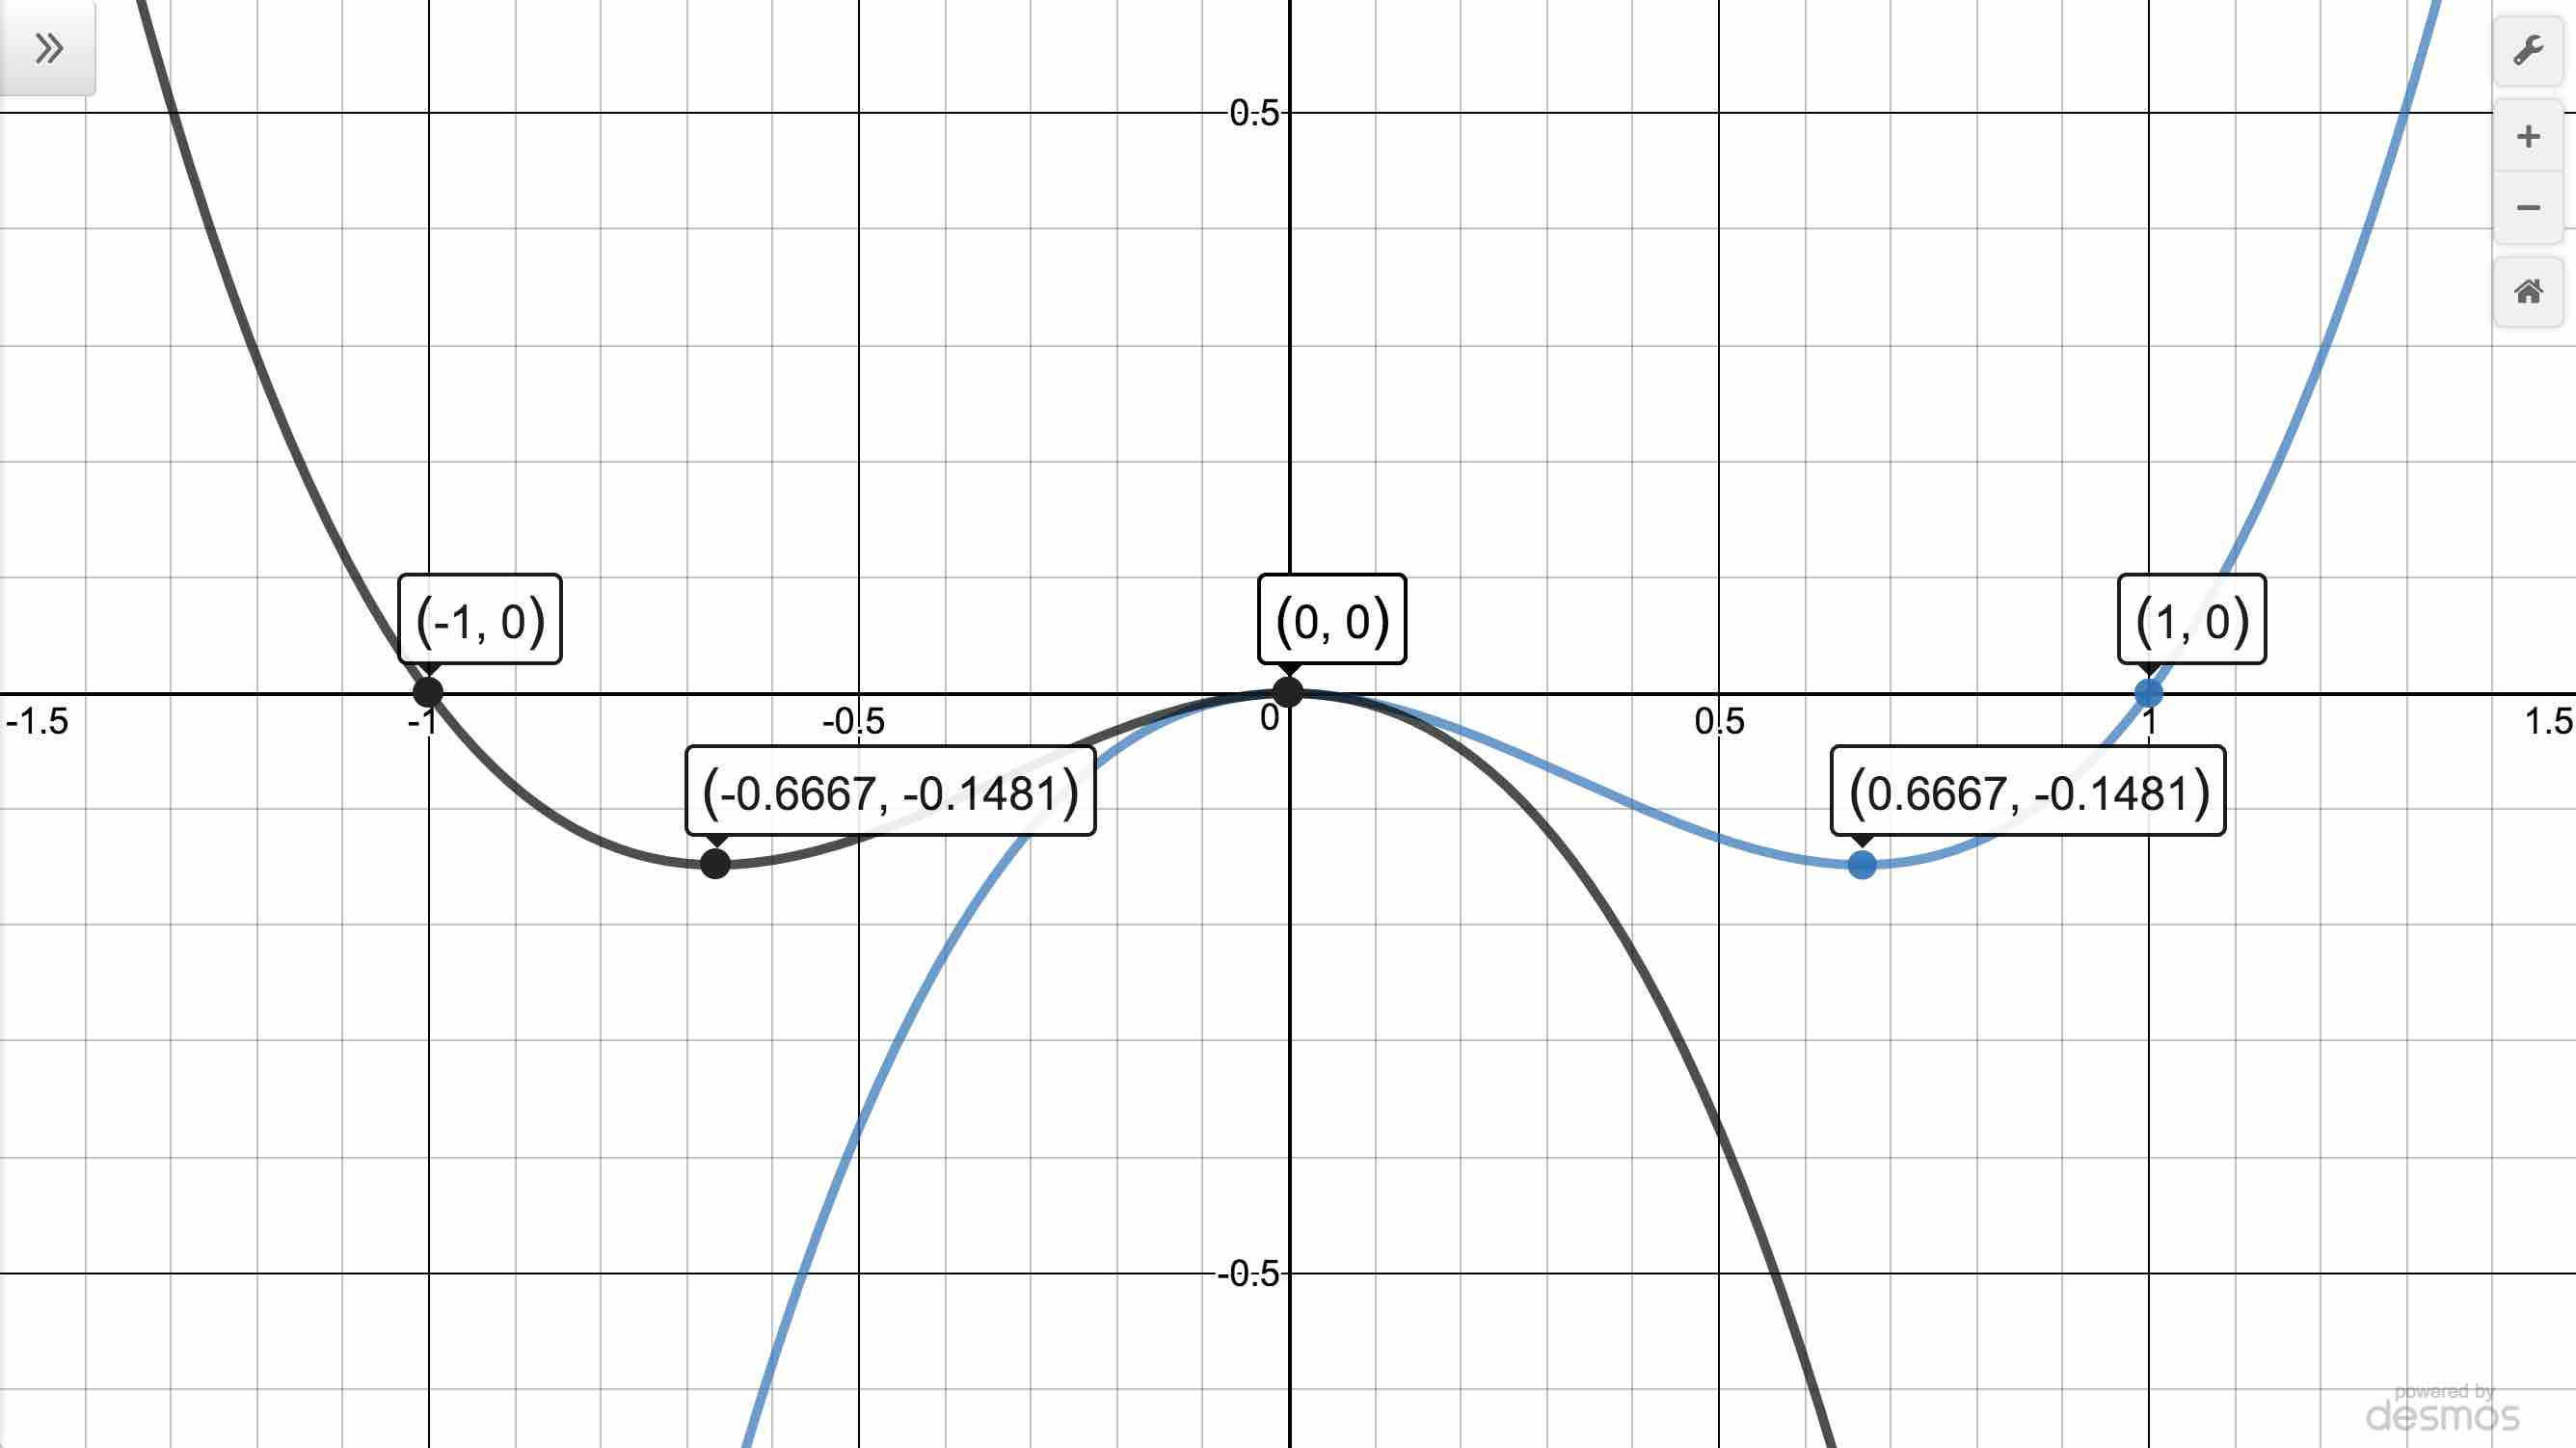
\includegraphics[width=3in]{./TransformationsGraphics/TransformationsEx02a.jpg} & 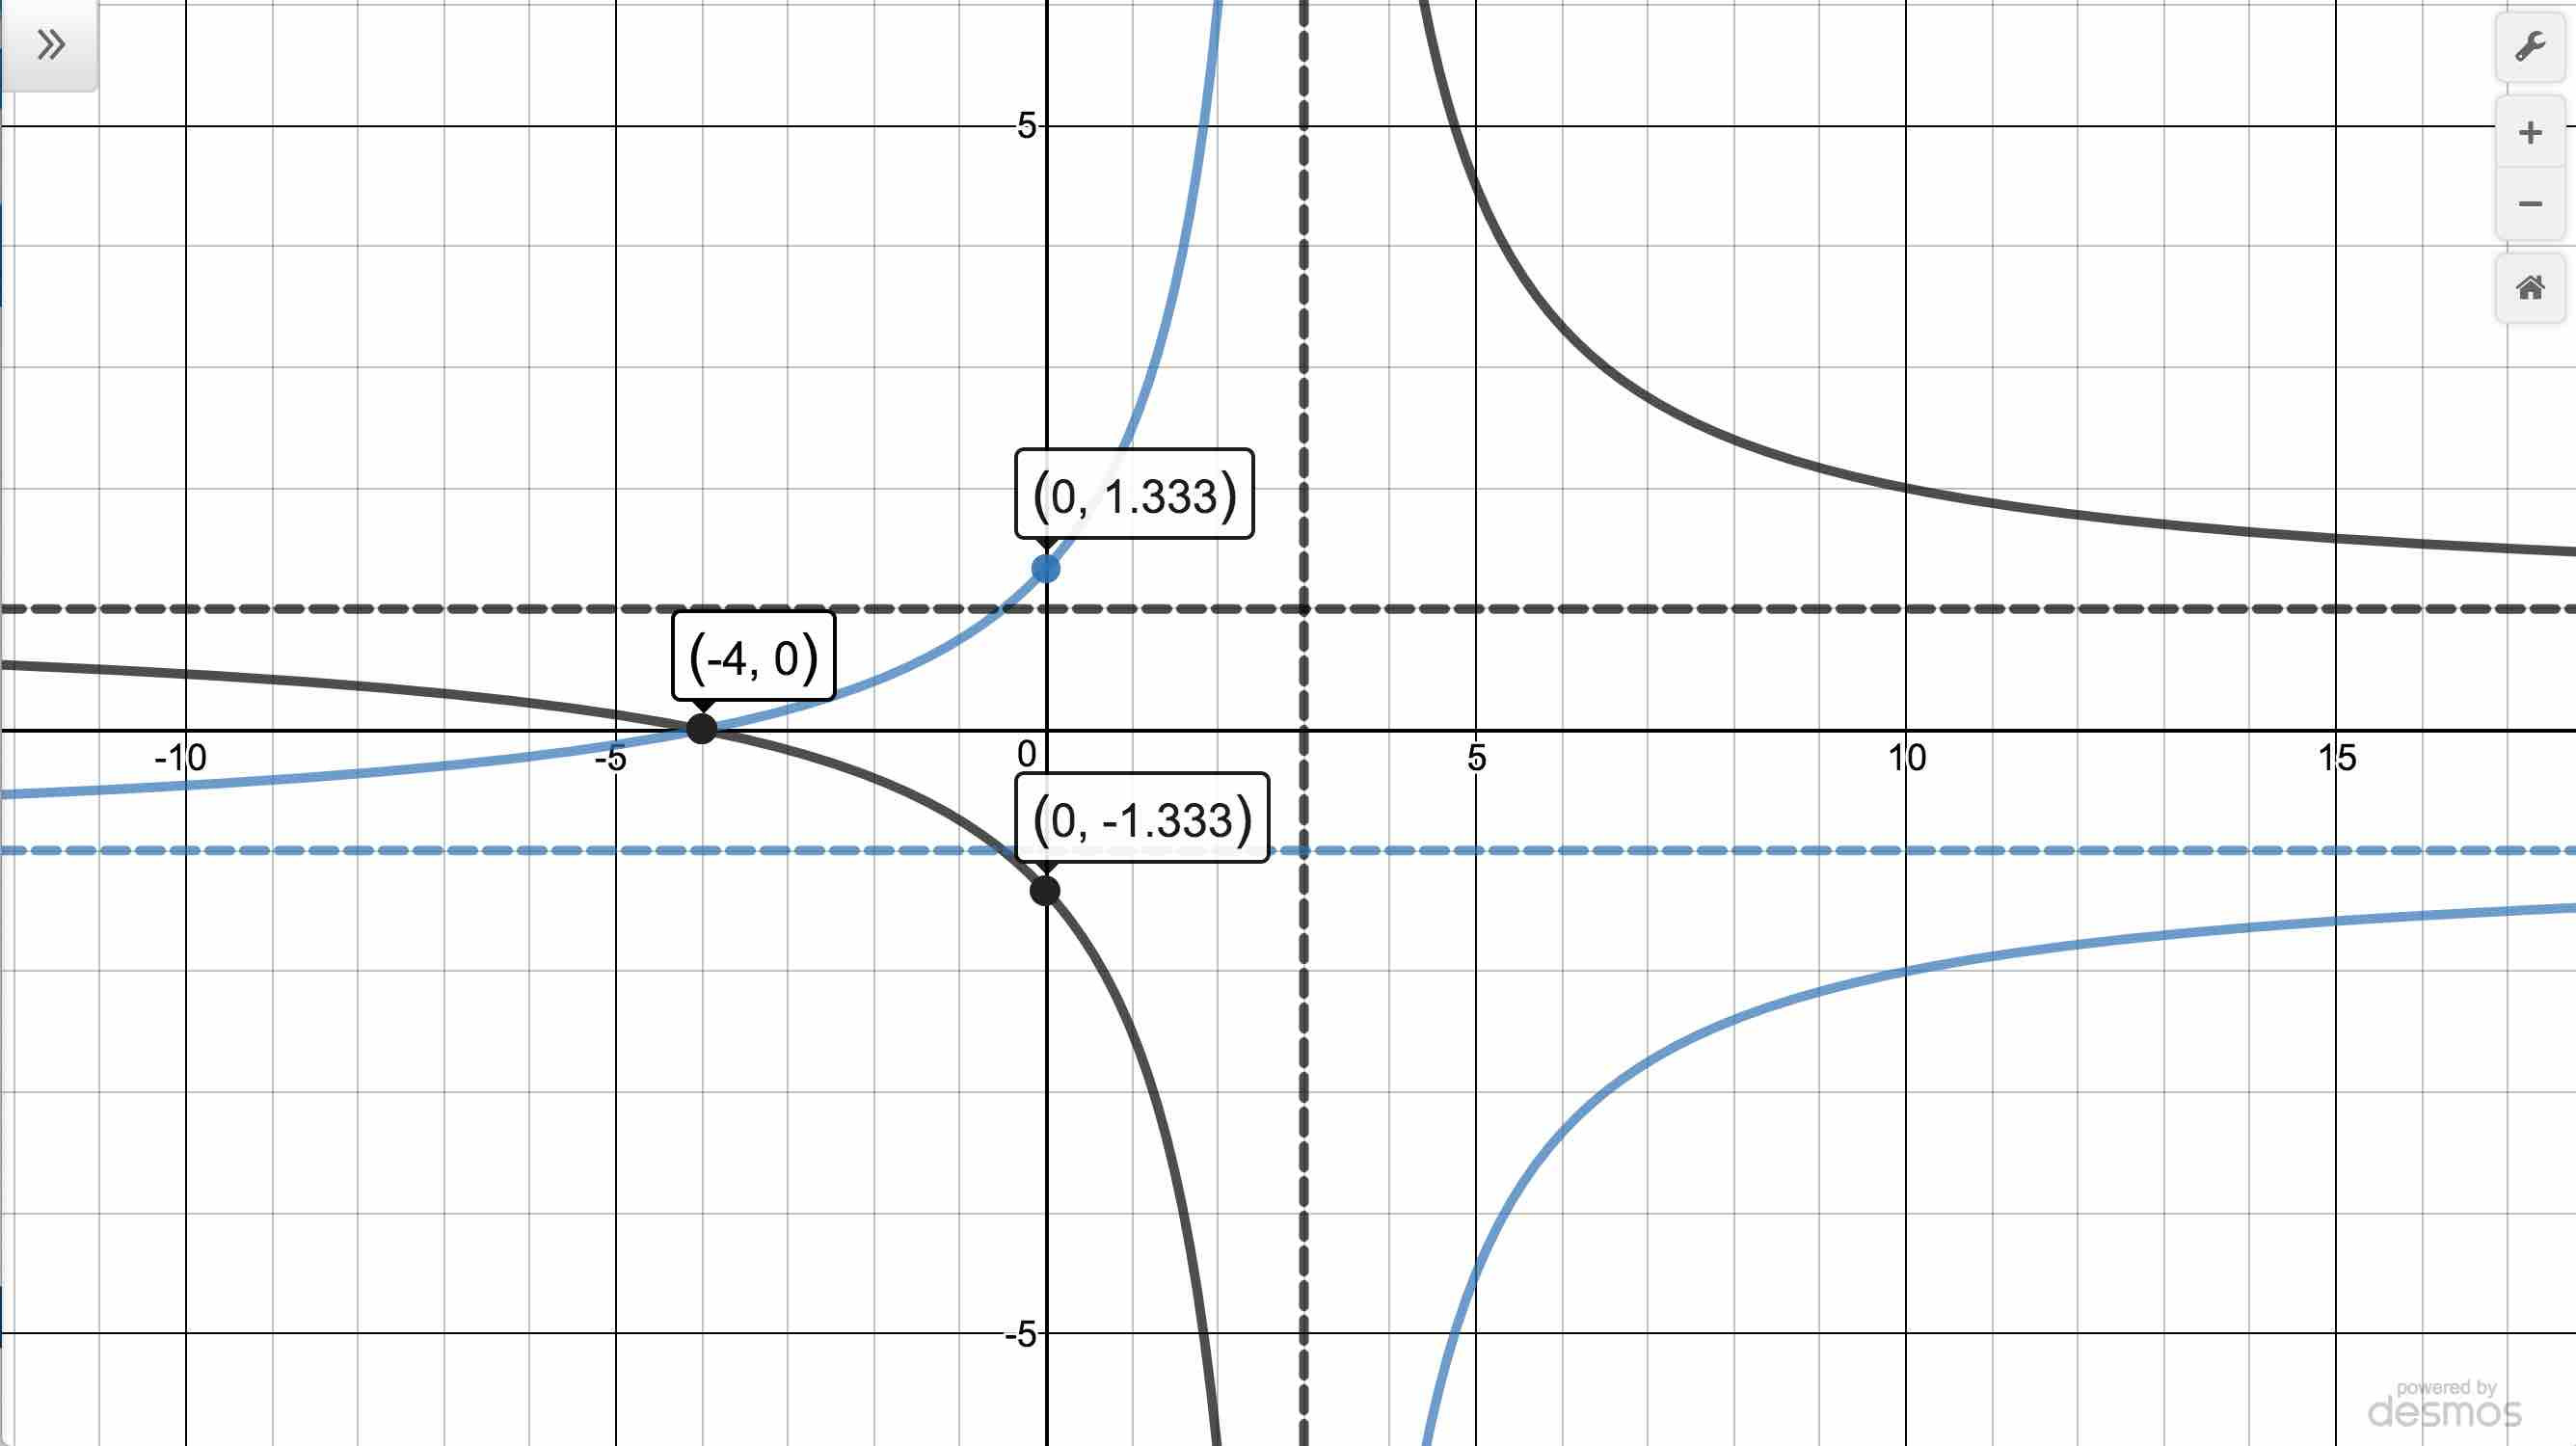
\includegraphics[width=3in]{./TransformationsGraphics/TransformationsEx02b.jpg} \\

$t =  s^3-s^2$ (lighter color)  and $t=-s^3-s^2$  &  $y = \dfrac{t+4}{3-t}$ (lighter color) and $y =  \dfrac{t+4}{t-3}$ \\

\end{tabular}

\end{center} 
 
\item
 
 \begin{enumerate}
 
 \item We have two transformations indicated with the formula $F(x) = f(-x)+1$:  a reflection across the $y$-axis and a vertical shift.  Working from the inside out, we first tackle the reflection.  Per Theorem \ref{reflections}, to obtain the graph of $y=f(-x)$ from $y=f(x)$, we multiply each of the $x$-coordinates of each of the points on the graph of $y=f(x)$ by $(-1)$.
 
 
 \[ \begin{array}{ccc}

\begin{mfpic}[15]{-3}{3}{-1}{6}
\axes
\tlabel[cc](3,-0.5){\scriptsize $x$}
\tlabel[cc](0.5,6){\scriptsize $y$}
\xmarks{-2, -1, 0, 1, 2}
\ymarks{ 0, 1, 2, 3,4,5}
\tcaption{\scriptsize $y = f(x)$}
\tlpointsep{4pt}
\scriptsize
\tlabel[cc](1, 1){$(0,1)$}
\tlabel[cc](2, 2){$(1,2)$}
\tlabel[cc](2.75, 4){$(2,4)$}
\axislabels {x}{{\scriptsize $-2 \hspace{7pt}$} -2,{\scriptsize $-1 \hspace{7pt}$} -1,{$1$} 1, {$2$} 2}
\axislabels {y}{{$2$} 2,{$3$} 3,{$4$} 4,{$5$} 5}
\normalsize
\penwd{1.25pt}
\arrow \reverse \arrow \function{-2.5, 2.5, 0.1}{2**x}
\point[4pt]{(0,1), (1,2), (2,4)}
\end{mfpic}


&

\stackrel{\stackrel{\mbox{\scriptsize reflect across $y$-axis}}{\xrightarrow{\hspace{1in}}}}{\mbox{ \scriptsize multiply each $x$-coordinate by $-1$}} 

&

\begin{mfpic}[15]{-3}{3}{-1}{6}
\axes
\tlabel[cc](3,-0.5){\scriptsize $x$}
\tlabel[cc](0.5,6){\scriptsize $y$}
\xmarks{-2, -1, 0, 1, 2}
\ymarks{ 0, 1, 2, 3,4,5}
\tcaption{\scriptsize $y = f(-x)$}
\tlpointsep{4pt}
\scriptsize
\tlabel[cc](-1, 1){$(0,1)$}
\tlabel[cc](-2.25, 2){$(-1,2)$}
\tlabel[cc](-3.25, 4){$(-2,4)$}
\axislabels {x}{{\scriptsize $-2 \hspace{7pt}$} -2,{\scriptsize $-1 \hspace{7pt}$} -1,{$1$} 1, {$2$} 2}
\axislabels {y}{{$2$} 2,{$3$} 3,{$4$} 4,{$5$} 5}
\normalsize
\penwd{1.25pt}
\arrow \reverse \arrow \function{-2.5, 2.5, 0.1}{2**(-x)}
\point[4pt]{(0,1), (-1,2), (-2,4)}
\end{mfpic}


\end{array}\]

Next, we use Theorem \ref{vshifts} to obtain the graph of $y =f(-x)+1$ from the graph of $y = f(-x)$ by adding $1$ to each of the $y$-coordinates of each of the points on the graph of $y = f(-x)$.  This shifts the graph of $y=f(-x)$ up one unit.  Note, the horizontal asymptote $y=0$ is also shifted up $1$ unit to $y=1$.

 
 \[ \begin{array}{ccc}

\begin{mfpic}[15]{-3}{3}{-1}{6}
\axes
\tlabel[cc](3,-0.5){\scriptsize $x$}
\tlabel[cc](0.5,6){\scriptsize $y$}
\xmarks{-2, -1, 0, 1, 2}
\ymarks{ 0, 1, 2, 3,4,5}
\tcaption{\scriptsize $y = f(-x)$}
\tlpointsep{4pt}
\scriptsize
\tlabel[cc](-1, 1){$(0,1)$}
\tlabel[cc](-2.25, 2){$(-1,2)$}
\tlabel[cc](-3.25, 4){$(-2,4)$}
\axislabels {x}{{\scriptsize $-2 \hspace{7pt}$} -2,{\scriptsize $-1 \hspace{7pt}$} -1,{$1$} 1, {$2$} 2}
\axislabels {y}{{$2$} 2,{$3$} 3,{$4$} 4,{$5$} 5}
\normalsize
\penwd{1.25pt}
\arrow \reverse \arrow \function{-2.5, 2.5, 0.1}{2**(-x)}
\point[4pt]{(0,1), (-1,2), (-2,4)}
\end{mfpic}


&

\stackrel{\stackrel{\mbox{\scriptsize shift up $1$ unit}}{\xrightarrow{\hspace{1in}}}}{\mbox{ \scriptsize add $1$ to each $y$-coordinate}} 

&

\begin{mfpic}[15]{-3}{3}{-1}{6}
\axes
\tlabel[cc](3,-0.5){\scriptsize $x$}
\tlabel[cc](0.5,6){\scriptsize $y$}
\xmarks{-2, -1, 0, 1, 2}
\ymarks{ 0, 1, 2, 3,4,5}
\tcaption{\scriptsize $y = f(-x)+1=F(x)$}
\tlpointsep{4pt}
\scriptsize
\tlabel[cc](-1, 2){$(0,2)$}
\tlabel[cc](-2.25, 3){$(-1,3)$}
\tlabel[cc](-3.25, 5){$(-2,5)$}
\axislabels {x}{{\scriptsize $-2 \hspace{7pt}$} -2,{\scriptsize $-1 \hspace{7pt}$} -1,{$1$} 1, {$2$} 2}
\axislabels {y}{{$3$} 3,{$4$} 4,{$5$} 5}
\normalsize
\dashed \polyline{(-3,1), (3,1)}
\penwd{1.25pt}
\arrow \reverse \arrow \function{-2.5, 2.5, 0.1}{2**(-x)+1}
\point[4pt]{(0,2), (-1,3), (-2,5)}
\end{mfpic}


\end{array}\]

To check our answer, we begin with the point $(0,2)$.  Substituting $x=0$ into $y=f(-x)+1$, we get $y=f(-0)+1 = f(0)+1$.  Since the point $(0,1)$ is on the graph of $f$, we know $f(0) = 1$.  Hence, $y = f(0)+1= 1+1=2$, so $(0,2)$ is, indeed, on the graph of $y=f(-x)+1$.  We leave it to the reader to check the remaining points.

 
  \item In order to graph $F(x)= 1 - f(2-x)$, we first rewrite as $F(x) = -f(-x+2)+1$ and note there are \textit{four} modifications to the formula $f(x)$ indicated here.  
  
  \smallskip
  
  Working from the inside out, we see we have a reflection about the $y$-axis indicated as well as a horizontal shift.  From our work above, we know we first handle the shift:  that is, we apply Theorem \ref{hshifts} to  graph $y=f(x+2) = f(x-(-2))$ by adding $-2$ to (subtracting $2$ from) the $x$-coordinates of the points on the graph of $y=f(x)$.
  
   \[ \begin{array}{ccc}

\begin{mfpic}[15]{-3}{3}{-1}{6}
\axes
\tlabel[cc](3,-0.5){\scriptsize $x$}
\tlabel[cc](0.5,6){\scriptsize $y$}
\xmarks{-2, -1, 0, 1, 2}
\ymarks{ 0, 1, 2, 3,4,5}
\tcaption{\scriptsize $y = f(x)$}
\tlpointsep{4pt}
\scriptsize
\tlabel[cc](1, 1){$(0,1)$}
\tlabel[cc](2, 2){$(1,2)$}
\tlabel[cc](2.75, 4){$(2,4)$}
\axislabels {x}{{\scriptsize $-2 \hspace{7pt}$} -2,{\scriptsize $-1 \hspace{7pt}$} -1,{$1$} 1, {$2$} 2}
\axislabels {y}{{$2$} 2,{$3$} 3,{$4$} 4,{$5$} 5}
\normalsize
\penwd{1.25pt}
\arrow \reverse \arrow \function{-2.5, 2.5, 0.1}{2**x}
\point[4pt]{(0,1), (1,2), (2,4)}
\end{mfpic}


&

\stackrel{\stackrel{\mbox{\scriptsize shift left $2$ units}}{\xrightarrow{\hspace{1in}}}}{\mbox{ \scriptsize subtract $2$ from each $x$-coordinate}} 

&

\begin{mfpic}[15]{-5}{1}{-1}{6}
\axes
\tlabel[cc](1,-0.5){\scriptsize $x$}
\tlabel[cc](0.5,6){\scriptsize $y$}
\xmarks{-4,-3, -2, -1, 0}
\ymarks{ 0, 1, 2, 3,4,5}
\tcaption{\scriptsize $y = f(x+2)$}
\tlpointsep{4pt}
\scriptsize
\tlabel[cc](-3.25, 1){$(-2,1)$}
\tlabel[cc](-2.25, 2){$(-1,2)$}
\tlabel[cc](-1, 4){$(0,4)$}
\axislabels {x}{{\scriptsize $-4 \hspace{7pt}$} -4,{\scriptsize $-3 \hspace{7pt}$} -3,{\scriptsize $-2 \hspace{7pt}$} -2,{\scriptsize $-1 \hspace{7pt}$} -1}
\axislabels {y}{{$2$} 2,{$5$} 5}
\normalsize
\penwd{1.25pt}
\arrow \reverse \arrow \function{-4.5, 0.5, 0.1}{2**(x+2)}
\point[4pt]{(-2,1), (-1,2), (0,4)}
\end{mfpic}


\end{array}\]

Next, we use Theorem \ref{reflections} to graph $y=f(-x+2)$ starting with the graph of $y = f(x+2)$ by multiplying each of the $x$-coordinates of the points of the graph of $y=f(x+2)$ by $-1$.  This reflects the graph of $f(x+2)$ about the $y$-axis.

 \[ \begin{array}{ccc}

\begin{mfpic}[15]{-5}{1}{-1}{6}
\axes
\tlabel[cc](1,-0.5){\scriptsize $x$}
\tlabel[cc](0.5,6){\scriptsize $y$}
\xmarks{-4,-3, -2, -1, 0}
\ymarks{ 0, 1, 2, 3,4,5}
\tcaption{\scriptsize $y = f(x+2)$}
\tlpointsep{4pt}
\scriptsize
\tlabel[cc](-3.25, 1){$(-2,1)$}
\tlabel[cc](-2.25, 2){$(-1,2)$}
\tlabel[cc](-1, 4){$(0,4)$}
\axislabels {x}{{\scriptsize $-4 \hspace{7pt}$} -4,{\scriptsize $-3 \hspace{7pt}$} -3,{\scriptsize $-2 \hspace{7pt}$} -2,{\scriptsize $-1 \hspace{7pt}$} -1}
\axislabels {y}{{$2$} 2,{$5$} 5}
\normalsize
\penwd{1.25pt}
\arrow \reverse \arrow \function{-4.5, 0.5, 0.1}{2**(x+2)}
\point[4pt]{(-2,1), (-1,2), (0,4)}
\end{mfpic}


&

\stackrel{\stackrel{\mbox{\scriptsize reflect about the $y$-axis}}{\xrightarrow{\hspace{1in}}}}{\mbox{ \scriptsize multiply each $x$-coordinate by $-1$}} 

&

\begin{mfpic}[15]{-1}{5}{-1}{6}
\axes
\tlabel[cc](5,-0.5){\scriptsize $x$}
\tlabel[cc](0.5,6){\scriptsize $y$}
\xmarks{0,1,2,3,4}
\ymarks{ 0, 1, 2, 3,4,5}
\tcaption{\scriptsize $y = f(-x+2)$}
\tlpointsep{4pt}
\scriptsize
\tlabel[cc](3, 1){$(2,1)$}
\tlabel[cc](1.75, 2){$(1,2)$}
\tlabel[cc](1, 4){$(0,4)$}
\axislabels {x}{{$1$} 1, {$2$} 2,{$3$} 3, {$4$} 4}
\axislabels {y}{{$2$} 2,{$3$} 3,{$4$} 4}
\normalsize
\penwd{1.25pt}
\arrow \reverse \arrow \function{-0.5, 4.5, 0.1}{2**(-x+2)}
\point[4pt]{(2,1), (1,2), (0,4)}
\end{mfpic}


\end{array}\]

We have the graph of $y=f(-x+2)$ and need to build towards the graph of $y=-f(-x+2)+1$.  The transformations that remain are a reflection about the $x$-axis and a vertical shift.  The question is which to do first.  

\smallskip

Once again, we can think algebraically about the problem.  We know the point $(0,1)$ is on the graph of $f$ which means $f(0) = 1$.  This point corresponds to the point $(2,1)$ on the graph of $f(-x+2)$.  Indeed, when we substitute $x=2$ into $y=f(-x+2)$, we get $y = f(-2+2) = f(0) =1$.  

\smallskip

If we substitute $x=2$ into the formula $y=-f(-x+2)+1$, we get $y=-f(-2+2)+1 = -f(0)+1  = -1(1)+1 = 0$.  That is, we first multiply the $y$-coordinate of $(2,1)$ by $-1$ then add $1$.  This suggests we take care of the reflection about the $x$-axis first, then the vertical shift.  

\smallskip

We proceed below to obtain the graph of $y=-f(-x+2)$ from $y=f(-x+2)$ by multiplying each of the $y$-coordinates on the graph of $y=f(-x+2)$ by $-1$.  Note the horizontal asymptote remains unchanged: $y=(-1)(0) = 0$.

 \[ \begin{array}{ccc}

\begin{mfpic}[15]{-1}{5}{-1}{6}
\axes
\tlabel[cc](5,-0.5){\scriptsize $x$}
\tlabel[cc](0.5,6){\scriptsize $y$}
\xmarks{0,1,2,3,4}
\ymarks{ 0, 1, 2, 3,4,5}
\tcaption{\scriptsize $y = f(-x+2)$}
\tlpointsep{4pt}
\scriptsize
\tlabel[cc](3, 1){$(2,1)$}
\tlabel[cc](1.75, 2){$(1,2)$}
\tlabel[cc](1, 4){$(0,4)$}
\axislabels {x}{{$1$} 1, {$2$} 2,{$3$} 3, {$4$} 4}
\axislabels {y}{{$2$} 2,{$3$} 3,{$4$} 4}
\normalsize
\penwd{1.25pt}
\arrow \reverse \arrow \function{-0.5, 4.5, 0.1}{2**(-x+2)}
\point[4pt]{(2,1), (1,2), (0,4)}
\end{mfpic}

&

\stackrel{\stackrel{\mbox{\scriptsize reflect about the $x$-axis}}{\xrightarrow{\hspace{1in}}}}{\mbox{ \scriptsize multiply each $y$-coordinate by $-1$}} 

&

\begin{mfpic}[15]{-1}{5}{-6}{1}
\axes
\tlabel[cc](5,-0.5){\scriptsize $x$}
\tlabel[cc](0.5,1){\scriptsize $y$}
\xmarks{0,1,2,3,4}
\ymarks{ 0, -1, -2, -3,-4,- 5}
\tcaption{\scriptsize $y = - f(-x+2)$}
\tlpointsep{4pt}
\scriptsize
\tlabel[cc](3, -1.25){$(2,-1)$}
\tlabel[cc](2, -2.25){$(1,-2)$}
\tlabel[cc](1, -4){$(0,-4)$}
\axislabels {x}{{$1$} 1, {$2$} 2}
\axislabels {y}{{$-2$} -2,{$-3$} -3,{$-4$} -4}
\normalsize
\penwd{1.25pt}
\arrow \reverse \arrow \function{-0.5, 4.5, 0.1}{0-2**(-x+2)}
\point[4pt]{(2,-1), (1,-2), (0,-4)}
\end{mfpic}

\end{array}\]

Finally, we take care of the vertical shift.  Per Theorem \ref{vshifts}, we graph $y=-f(-x+2)+1$ by adding $1$ to the $y$-coordinates of each of the points on the graph of $y=-f(-x+2)$.  This moves the graph up one unit, including the horizontal asymptote:  $y=0+1 = 1$.

 \[ \begin{array}{ccc}

\begin{mfpic}[15]{-1}{5}{-6}{1}
\axes
\tlabel[cc](5,-0.5){\scriptsize $x$}
\tlabel[cc](0.5,1){\scriptsize $y$}
\xmarks{0,1,2,3,4}
\ymarks{ 0, -1, -2, -3,-4,- 5}
\tcaption{\scriptsize $y = - f(-x+2)$}
\tlpointsep{4pt}
\scriptsize
\tlabel[cc](3, -1.25){$(2,-1)$}
\tlabel[cc](2, -2.25){$(1,-2)$}
\tlabel[cc](1, -4){$(0,-4)$}
\axislabels {x}{{$1$} 1, {$2$} 2}
\axislabels {y}{{$-2$} -2,{$-3$} -3,{$-4$} -4}
\normalsize
\penwd{1.25pt}
\arrow \reverse \arrow \function{-0.5, 4.5, 0.1}{0-2**(-x+2)}
\point[4pt]{(2,-1), (1,-2), (0,-4)}
\end{mfpic}

&

\stackrel{\stackrel{\mbox{\scriptsize shift up $1$ unit}}{\xrightarrow{\hspace{1in}}}}{\mbox{ \scriptsize add $1$ to each of the $y$-coordinates}} 

&

\begin{mfpic}[15]{-1}{5}{-5}{2}
\axes
\tlabel[cc](5,-0.5){\scriptsize $x$}
\tlabel[cc](0.5,2){\scriptsize $y$}
\xmarks{0,1,2,3,4}
\ymarks{ 1, 0, -1, -2, -3,-4}
\tcaption{\scriptsize $y = - f(-x+2)+1 = F(x)$}
\tlpointsep{4pt}
\scriptsize
\tlabel[cc](2.5, -0.5){$(2,0)$}
\tlabel[cc](2, -1.25){$(1,-1)$}
\tlabel[cc](1, -3){$(0,-3)$}
\axislabels {x}{{$1$} 1}
\axislabels {y}{{$-2$} -2,{$-3$} -3,{$1$} 1}
\normalsize
\dashed \polyline{(-1,1), (5,1)}
\penwd{1.25pt}
\arrow \reverse \arrow \function{-0.5, 4.5, 0.1}{1-2**(-x+2)}
\point[4pt]{(2,0), (1,-1), (0,-3)}
\end{mfpic}

\end{array}\]

To check, we begin with the point $(2,0)$.  Substituting $x=2$ into $y=1 - f(2-x)$, we obtain $y = 1-f(2-2) = 1-f(0)$.  Since $(0,1)$ is on the graph of $f$, we know $f(0) = 1$.  This means $y = 1-f(2-2) = 1-f(0)= 1-1 = 0$.  This proves $(2,0)$ is on the graph of  $y=1 - f(2-x)$, and we recommend the reader check the remaining points.
 
 \end{enumerate}

 \item With the transformations at our disposal,  our task amounts to finding values of $h$ and $k$ and choosing between signs $\pm$  so that  $g(x) = \pm f( \pm x - h) + k$.  
 
 \smallskip
 
 Based on the horizontal asymptote, $y=4$, we choose $k=4$.  Note, however, in the graph of $y=f(x)+4$, the entire graph is \textit{above} the line $y=4$.  Since the graph of $g$ approaches the asymptote from below, we know  $y=-f(\pm x-h)+4$.  
 
 \smallskip
 
 Hence, two of transformations applied to the graph of $f$ are a reflection across the $x$-axis followed by a shift up $4$ units.  This means the point $(0,1)$ on the graph of $f$ must correspond to the point $(-1,3)$ on the graph of $g$, since these are the points closest to the asymptote on each graph.  
  
  \smallskip
  
Likewise, the points $(1,2)$ and $(2,4)$ on the graph of $f$ must correspond to $(0,2)$ and $(1,0)$, respectively, on the graph of $g$.  Looking at the $x$-coordinates only, we have $x=0$ moves to $x=-1$, $x=1$ moves to $x=0$, and $x=2$ moves to $x=1$.  Hence, the net effect on the $x$-values is a shift left $1$ unit.  Hence, we guess the formula for $g(x)$ to be $g(x) = -f(x+1)+4$.  

\smallskip

We can readily check by going through the transformations:  first, shift left $1$ unit; next,  reflect across the $x$-axis;  finally, shift up $4$.  We leave it to the reader to verify that tracking each of the points on the graph of $f$ along with the horizontal asymptote through this sequence of transformations results in the graph of $g$.  
 
 
 \smallskip
 
 
 One way to recover the graph of $f$ from the graph of $g$ is to reverse the process by which we obtained $g$ from $f$.  The challenge here comes from the fact that two different operations were done which affected the $y$-values:  reflection and shifting - and the order in which these are done matters.  
 
 \smallskip
 
 To motivate our methodology, let's consider a more down-to-earth example like putting on socks and then putting on shoes.  Unless we're very talented,  to reverse this process, we take off the shoes first, then the socks - that is, we undo each step in the reverse order.\footnote{We'll have more to say about this sort of thing in Section \ref{InverseFunctions}.}  In the same way, when we think about reversing the steps transforming the graph of $f$ to the graph of $g$, we need to undo each transformation in the opposite order.  
 
 \smallskip
 
 To review, we obtained the graph of $g$ from the graph of $f$ by first shifting the graph to the left $1$ unit, then reflecting the graph about the $x$-axis, then, finally, shifting the graph up $4$ units.  Hence, we first undo the vertical shift.  Instead of shifting the graph \textit{up} four units, we shift the graph \textit{down} four units.  This takes the graph of $y = g(x)$ to $y = g(x)-4$.  
 
 \smallskip
 
 Next, we have to undo the refection across the $x$-axis.  Thinking at the level of points, to recover the point $(a,b)$ from its reflection across the $x$-axis, $(a,-b)$, we simply reflect across the $x$-axis again: $(a,-(-b)) = (a,b)$.  Per Theorem \ref{reflections}, this takes the graph the graph of $y = g(x)-4$ to the graph of $y = -[g(x)-4] = -g(x) + 4$.\footnote{To see this better, let us temporarily write $F(x) = g(x)-4$.  Theorem \ref{reflections} tells us to reflect the graph of $F$ about the $x$-axis, graph $y=-F(x) = - [g(x)-4] = -g(x)+4$.} 
 
 \smallskip
 
 Last, to undo moving the graph to the \textit{left} $1$ unit, we move the graph of $y=-g(x)+4$ to the \textit{right} $1$ unit.  Per Theorem \ref{hshifts}, we accomplish this by graphing $y = -g(x-1)+4$.  We leave it to the reader to start with the graph of $y=g(x)$ and graph $y = -g(x-1)+4$ and show it matches the graph of $y=f(x)$. \qed
    
 \end{enumerate}

\end{ex}

Some remarks about Example \ref{reflectionsex}  are in order. In number \ref{twotransxrefex} above, to find a point on the graph of $y=f(-x+8)$, we took the given $x$-coordinate on our starting graph, $2$, and subtracted $8$ first then multiplied by $-1$.  If this seems somehow `backwards' it should.  

\smallskip

When \textit{evaluating} the expression $-x+8$, the order of operations mandates we multiply by $-1$ first then add $8$.  Here, however, we weren't \textit{evaluating} an expression - we were \textit{solving} an equation:  $-x+8 = 2$, which meant we did the exact opposite steps in the opposite order.\footnote{Note that dividing by $-1$ is the same as multiplying by $-1$, so to keep with the `opposite steps in opposite order' theme, we could more precisely say we subtracted $8$ and \textit{divided} by $-1$.}  This exemplifies a larger theme with transformations:  when adjusting inputs, the resulting points on the graph are obtained by applying the opposite operations indicated by the formula in the opposite order of operations.



\smallskip


On the other hand, when it came to multiple transformations involving the $y$-coordinates, we followed the order of operations. As in \ref{twotransyrefex} above, when it came to applying a reflection about the $x$-axis and a vertical shift, we applied the reflection first, then the shift.  This is because instead of \textit{solving} an \textit{equation} to find the new $y$-coordinates, we were \textit{simplifying }an \textit{expression}.  Again, this is an example of a much larger theme:  when adjusting outputs, the resulting points on the graph are obtained by applying the stated operations in the usual order.


\smallskip


Last but not least, in number \ref{gfromfrefex}, to find $f$ in terms of $g$, we reversed the steps used to transform $f$ into $g$.  Another tact is to approach the problem in the same way we approached transforming $f$ into $g$: namely, starting with the graph of $g$, determine values $h$ and $k$ and signs $\pm$ so that $f(x) = \pm g(\pm x - h) + k$.  We leave this to the reader.


\subsection{Scalings}
\label{Scaling}

We now turn our attention to our last class of transformations: \textbf{scalings}.  A thorough discussion of scalings can get complicated because they are not as straight-forward as the previous transformations.  A quick review of what we've covered so far, namely vertical shifts, horizontal shifts and reflections, will show you why those transformations are known as \index{transformation ! rigid}\textbf{rigid transformations}.  

\smallskip

Simply put, rigid transformations preserve the distances between points on the graph -  only their position and orientation in the plane change.\footnote{Another word that can be used here instead of `rigid transformation' is `isometry' - meaning `same distance.'}  If, however, we wanted to make a new graph twice as tall as a given graph, or one-third as wide, we would be affecting the distance between points. These sorts of transformations are hence called \textbf{non-rigid}\index{transformation ! non-rigid}.  As always, we motivate the general theory with an example.

\smallskip

Suppose we wish to graph the function $g(x) =2 f(x)$ where $f(x)$ is the function whose graph is given at the beginning of the section. From its graph, we can build a table of values for $g$ as before.

\begin{center}

\begin{tabular}{m{2in}m{3in}}

\begin{mfpic}[15]{-1}{6}{-1}{6}
\tlabel[cc](-1,1){\scriptsize $(0,1)$}
\tlabel[cc](2,3.5){\scriptsize $(2,3)$}
\tlabel[cc](4,2.5){\scriptsize $(4,3)$}
\tlabel[cc](5,5.5){\scriptsize $(5,5)$}
\tlabel[cc](6,-0.5){\scriptsize $x$}
\tlabel[cc](0.5,6){\scriptsize $y$}
\tcaption{\scriptsize $y=f(x)$}
\axes
\xmarks{1,2,3,4,5}
\ymarks{1,2,3,4,5}
\tlpointsep{4pt}
\axislabels {x}{{\scriptsize $1$} 1, {\scriptsize $2$} 2, {\scriptsize $3$} 3, {\scriptsize $4$} 4, {\scriptsize $5$} 5}
\axislabels {y}{{\scriptsize $2$} 2, {\scriptsize $3$} 3, {\scriptsize $4$} 4, {\scriptsize $5$} 5}
\penwd{1.25pt}
\polyline{(0,1), (2,3), (4,3), (5,5)}
\point[4pt]{(0,1), (2,3), (4,3), (5,5)}
\end{mfpic}
 
&

\[ \begin{array}{|c||c|c|c|c|}  

\hline

 x & (x,f(x)) & f(x) & g(x)=2f(x) & (x, g(x)) \\ \hline
0  & (0,1)& 1 & 2 &(0, 2) \\  \hline
2 & (2,3) & 3 &  6 &(2,6) \\  \hline
4 & (4,3) & 3 &  6 &(4, 6) \\  \hline
5 & (5,5) & 5 &  10 &( 5 ,10) \\  \hline

\end{array} \] 

\end{tabular}

\end{center}

Graphing, we get:

\[ \begin{array}{ccc}

\begin{mfpic}[15]{-1}{6}{-1}{11}
\tlabel[cc](-1,1){\scriptsize $(0,1)$}
\tlabel[cc](2,3.5){\scriptsize $(2,3)$}
\tlabel[cc](4,2.5){\scriptsize $(4,3)$}
\tlabel[cc](5,5.5){\scriptsize $(5,5)$}
\tlabel[cc](6,-0.5){\scriptsize $x$}
\tlabel[cc](0.5,11){\scriptsize $y$}
\tcaption{\scriptsize $y=f(x)$}
\axes
\xmarks{1,2,3,4,5}
\ymarks{1,2,3,4,5,6,7,8,9,10}
\tlpointsep{4pt}
\axislabels {x}{{\scriptsize $1$} 1, {\scriptsize $2$} 2, {\scriptsize $3$} 3, {\scriptsize $4$} 4, {\scriptsize $5$} 5}
\axislabels {y}{{\scriptsize $2$} 2, {\scriptsize $3$} 3, {\scriptsize $4$} 4, {\scriptsize $5$} 5, {\scriptsize $6$} 6, {\scriptsize $7$} 7, {\scriptsize $8$} 8, {\scriptsize $9$} 9,  {\scriptsize $10$} 10 }
\penwd{1.25pt}
\polyline{(0,1), (2,3), (4,3), (5,5)}
\point[4pt]{(0,1), (2,3), (4,3), (5,5)}
\end{mfpic}

&

\stackrel{\stackrel{\mbox{\scriptsize vertical scaling by a factor of $2$ }}{\xrightarrow{\hspace{1.7in}}}}{\mbox{ \scriptsize multiply each $y$-coordinate by $2$}} 

&


\begin{mfpic}[15]{-1}{6}{-1}{11}
\tlabel[cc](-1,2){\scriptsize $(0,2)$}
\tlabel[cc](2,6.5){\scriptsize $(2,6)$}
\tlabel[cc](4,5.5){\scriptsize $(4,6)$}
\tlabel[cc](5,10.5){\scriptsize $(5,10)$}
\tlabel[cc](6,-0.5){\scriptsize $x$}
\tlabel[cc](0.5,11){\scriptsize $y$}
\tcaption{\scriptsize $y= 2f(x)$}
\axes
\xmarks{1,2,3,4,5}
\ymarks{1,2,3,4,5,6,7,8,9,10}
\tlpointsep{4pt}
\axislabels {x}{{\scriptsize $1$} 1, {\scriptsize $2$} 2, {\scriptsize $3$} 3, {\scriptsize $4$} 4, {\scriptsize $5$} 5}
\axislabels {y}{{\scriptsize $1$} 1, {\scriptsize $3$} 3, {\scriptsize $4$} 4, {\scriptsize $5$} 5, {\scriptsize $6$} 6, {\scriptsize $7$} 7, {\scriptsize $8$} 8, {\scriptsize $9$} 9,  {\scriptsize $10$} 10 }
\penwd{1.25pt}
\polyline{(0,2), (2,6), (4,6), (5,10)}
\point[4pt]{(0,2), (2,6), (4,6), (5,10)}
\end{mfpic}

\end{array} \]

In general, if $(a,b)$ is on the graph of $f$, then $f(a) = b$ so that $g(a) = 2 f(a) = 2b$ puts $(a,2b)$ on the graph of $g$.  In other words, to obtain the graph of $g$, we multiply all of the $y$-coordinates of the points on the graph of $f$ by $2$.  Multiplying all of the $y$-coordinates of all of the points on the graph of $f$ by $2$ causes what is known as a `vertical scaling\footnote{Also called a `vertical stretch,' `vertical expansion' or `vertical dilation' by a factor of $2$.} by a factor of $2$.'

\smallskip

If we wish to graph $y = \frac{1}{2} f(x)$, we multiply the all of the $y$-coordinates of the points on the graph of $f$ by $\frac{1}{2}$.  This creates a `vertical scaling\footnote{Also called `vertical shrink,' `vertical compression' or `vertical contraction' by a factor of $2$.} by a factor of $\frac{1}{2}$' as seen below.

\[ \begin{array}{ccc}

\begin{mfpic}[15]{-1}{6}{-1}{6}
\tlabel[cc](-1,1){\scriptsize $(0,1)$}
\tlabel[cc](2,3.5){\scriptsize $(2,3)$}
\tlabel[cc](4,2.5){\scriptsize $(4,3)$}
\tlabel[cc](5,5.5){\scriptsize $(5,5)$}
\tlabel[cc](6,-0.5){\scriptsize $x$}
\tlabel[cc](0.5,6){\scriptsize $y$}
\tcaption{\scriptsize $y=f(x)$}
\axes
\xmarks{1,2,3,4,5}
\ymarks{1,2,3,4,5}
\tlpointsep{4pt}
\axislabels {x}{{\scriptsize $1$} 1, {\scriptsize $2$} 2, {\scriptsize $3$} 3, {\scriptsize $4$} 4, {\scriptsize $5$} 5}
\axislabels {y}{{\scriptsize $2$} 2, {\scriptsize $3$} 3, {\scriptsize $4$} 4, {\scriptsize $5$} 5}
\penwd{1.25pt}
\polyline{(0,1), (2,3), (4,3), (5,5)}
\point[4pt]{(0,1), (2,3), (4,3), (5,5)}
\end{mfpic}

&

\stackrel{\stackrel{\mbox{\scriptsize vertical scaling by a factor of $\frac{1}{2}$ }}{\xrightarrow{\hspace{1.7in}}}}{\mbox{ \scriptsize multiply each $y$-coordinate by $\frac{1}{2}$}} 

&

\begin{mfpic}[15]{-1}{6}{-1}{6}
\tlabel[cc](-1,0.5){\scriptsize $\left(0,\frac{1}{2}\right)$}
\tlabel[cc](2,2){\scriptsize $\left(2,\frac{3}{2}\right)$}
\tlabel[cc](4,1){\scriptsize $\left(4,\frac{3}{2}\right)$}
\tlabel[cc](5,3){\scriptsize $\left(5,\frac{5}{2}\right)$}
\tlabel[cc](6,-0.5){\scriptsize $x$}
\tlabel[cc](0.5,6){\scriptsize $y$}
\tcaption{\scriptsize $y=\frac{1}{2} f(x)$}
\axes
\xmarks{1,2,3,4,5}
\ymarks{1,2,3,4,5}
\tlpointsep{4pt}
\axislabels {x}{{\scriptsize $1$} 1, {\scriptsize $2$} 2, {\scriptsize $3$} 3, {\scriptsize $4$} 4, {\scriptsize $5$} 5}
\axislabels {y}{{\scriptsize $1$} 1,{\scriptsize $2$} 2, {\scriptsize $3$} 3, {\scriptsize $4$} 4, {\scriptsize $5$} 5}
\penwd{1.25pt}
\polyline{(0,0.5), (2,1.5), (4,1.5), (5,2.5)}
\point[4pt]{(0,0.5), (2,1.5), (4,1.5), (5,2.5)}
\end{mfpic}

\end{array} \]

These results are generalized in the following theorem.

\smallskip

\colorbox{ResultColor}{\bbm

%\smallskip

\begin{thm} \label{vscalings}\index{graph ! vertical scaling}\textbf{Vertical Scalings.} Suppose $f$ is a function and $a>0$ is a real number. 

To graph $F(x) = af(x)$, multiply each of the $y$-coordinates of the points on the graph of $y=f(x)$ by $a$. 

\begin{itemize}

\item If $a > 1$, we say the graph of $f$ has undergone a vertical stretch\footnote{expansion, dilation} by a factor of $a$. 

\item If $0 < a < 1$, we say the graph of $f$ has undergone a vertical shrink\footnote{ compression, contraction} by a factor of $\frac{1}{a}$.

\end{itemize}

\end{thm}

\ebm}

\smallskip

The proof of Theorem \ref{vscalings} mimics the proofs of Theorems \ref{vshifts} and \ref{reflections}.  If $c$ is in the domain of $f$, then $(c, f(c))$ is on the graph of $f$ and the corresponding point on the graph of $F(x)=af(x)$ is $(c, F(c)) = (c, a f(c))$.  Comparing the points $(c, f(c))$ and $(c, a f(c))$ proves the theorem.  

\smallskip

A few remarks about Theorem \ref{vscalings} are in order.  First, a note about the verbiage.  To the authors, the words `stretch', `expansion', and `dilation' all indicate something getting bigger.  Hence, `stretched by a factor of $2$' makes sense if we are scaling something by multiplying it by $2$. Similarly, we believe words like `shrink', `compression' and `contraction' all indicate something getting smaller, so if we scale something by a factor of $\frac{1}{2}$, we would say it `shrinks by a factor of $2$' - not `shrinks by a factor of $\frac{1}{2}$'.  This is why we have written the descriptions `stretch by a factor of $a$' and `shrink by a factor of $\frac{1}{a}$' in the statement of the theorem.  

\smallskip

Second, in terms of inputs and outputs, Theorem \ref{vscalings} says multiplying the \textit{outputs} from a function by positive number $a$ causes the graph to be vertically scaled by a factor of $a$.  It is natural to ask what would happen if we multiply the \textit{inputs} of a function by a positive number.  This leads us to our last transformation of the section.

\smallskip

Referring to the graph of $f$ given at the beginning of this section, suppose we want to graph $g(x) = f(2x)$.  In other words, we are looking to see what effect multiplying the inputs to $f$ by $2$ has on its graph.  If we attempt to build a table directly, we quickly run into the same problem we had in our discussion leading up to Theorem \ref{hshifts}, as seen in the table on the left below.  

\smallskip

We solve this problem in the same way we solved this problem before.  For example, if we want to determine the point on $g$ which corresponds to the point $(2,3)$ on the graph of $f$,  we set $2x =2 $ so that $x=1$.  Substituting $x=1$ into $g(x)$, we obtain $g(1) = f(2 \cdot 1) = f(2) = 3$, so that $(1,3)$ is on the graph of $g$. Continuing in this fashion, we obtain the table on the lower right.   

\smallskip

\begin{tabular}{cc}

$ \begin{array}{|c||c|c|c|c|}  

\hline

x & (x,f(x)) & f(x)& g(x)=f(2x) & (x, g(x)) \\ \hline
0  & (0,1)& 1 & f(2 \cdot 0) = f(0) = 1   &(0, 1) \\  \hline
2 & (2,3) & 3 & f(2\cdot2) = f(4) = 3  &(2,3) \\  \hline
4 & (4,3) & 3 &  f(2 \cdot 4) = f(8) = ? &  \\  \hline
5 & (5,5) & 5 & f(2 \cdot 5) = f(10) = ?  &  \\  \hline

\end{array} $ 

&

$ \begin{array}{|r||c|c|c|}  

\hline

x & 2x & g(x)=f(2x) & (x, g(x)) \\ \hline
0 & 0 & g(0)= f(2 \cdot 0) = f(0) = 1   &(0, 0) \\  \hline
1 &  2 &  g(1)=f(2 \cdot 1) = f(2)  = 3  &(1,3) \\  \hline
2 & 4  & g(2)=f(2 \cdot 2) = f(4) = 3 &  (2,3)\\  \hline
\frac{5}{2}  & 5 & g\left(\frac{5}{2}\right)=f\left(2 \cdot \frac{5}{2} \right) = f(5) = 5  & \left(\frac{5}{2},5\right) \\ [1pt] \hline

\end{array} $

\end{tabular} 

\smallskip

In general, if $(a,b)$ is on the graph of $f$, then $f(a) = b$.  Hence $g\left(\frac{a}{2}\right) = f\left(2 \cdot \frac{a}{2}\right) = f(a) = b$ so that $\left(\frac{a}{2}, b\right)$ is on the graph of $g$.  In other words, to graph $g$ we divide the $x$-coordinates of the points on the graph of $f$ by $2$.  This results in a horizontal scaling\footnote{Also called `horizontal shrink,' `horizontal compression' or `horizontal contraction' by a factor of $2$.} by a factor of $\frac{1}{2}$.

\[ \begin{array}{ccc}

\begin{mfpic}[15]{-1}{6}{-1}{6}
\tlabel[cc](-1,1){\scriptsize $(0,1)$}
\tlabel[cc](2,3.5){\scriptsize $(2,3)$}
\tlabel[cc](4,2.5){\scriptsize $(4,3)$}
\tlabel[cc](5,5.5){\scriptsize $(5,5)$}
\tlabel[cc](6,-0.5){\scriptsize $x$}
\tlabel[cc](0.5,6){\scriptsize $y$}
\tcaption{\scriptsize $y=f(x)$}
\axes
\xmarks{1,2,3,4,5}
\ymarks{1,2,3,4,5}
\tlpointsep{4pt}
\axislabels {x}{{\scriptsize $1$} 1, {\scriptsize $2$} 2, {\scriptsize $3$} 3, {\scriptsize $4$} 4, {\scriptsize $5$} 5}
\axislabels {y}{{\scriptsize $2$} 2, {\scriptsize $3$} 3, {\scriptsize $4$} 4, {\scriptsize $5$} 5}
\penwd{1.25pt}
\polyline{(0,1), (2,3), (4,3), (5,5)}
\point[4pt]{(0,1), (2,3), (4,3), (5,5)}
\end{mfpic}

&

\stackrel{\stackrel{\mbox{\scriptsize horizontal scaling by a factor of $\frac{1}{2}$ }}{\xrightarrow{\hspace{1.7in}}}}{\mbox{ \scriptsize multiply each $x$-coordinate by $\frac{1}{2}$}} 

&

\begin{mfpic}[15]{-1}{6}{-1}{6}
\tlabel[cc](-1,1){\scriptsize $(0,1)$}
\tlabel[cc](1,3.5){\scriptsize $(1,3)$}
\tlabel[cc](2,2.5){\scriptsize $(2,3)$}
\tlabel[cc](2.5,5.5){\scriptsize $\left(\frac{5}{2},5\right)$}
\tlabel[cc](6,-0.5){\scriptsize $x$}
\tlabel[cc](0.5,6){\scriptsize $y$}
\tcaption{\scriptsize $y=g(x) = f(2x)$}
\axes
\xmarks{1,2,3,4,5}
\ymarks{1,2,3,4,5}
\tlpointsep{4pt}
\axislabels {x}{{\scriptsize $1$} 1, {\scriptsize $2$} 2, {\scriptsize $3$} 3, {\scriptsize $4$} 4, {\scriptsize $5$} 5}
\axislabels {y}{{\scriptsize $2$} 2, {\scriptsize $3$} 3, {\scriptsize $4$} 4, {\scriptsize $5$} 5}
\penwd{1.25pt}
\polyline{(0,1), (1,3), (2,3), (2.5,5)}
\point[4pt]{(0,1), (1,3), (2,3), (2.5,5)}
\end{mfpic}

\end{array}\]

If, on the other hand, we wish to graph $y = f\left( \frac{1}{2} x\right)$, we end up multiplying the $x$-coordinates of the points on the graph of $f$ by $2$ which results in a horizontal scaling\footnote{Also called `horizontal stretch,'  `horizontal expansion' or `horizontal dilation' by a factor of $2$.} by a factor of $2$, as demonstrated below.

\[ \begin{array}{ccc}

\begin{mfpic}[12]{-1}{11}{-1}{6}
\tlabel[cc](-1,1){\scriptsize $(0,1)$}
\tlabel[cc](2,3.5){\scriptsize $(2,3)$}
\tlabel[cc](4,2.5){\scriptsize $(4,3)$}
\tlabel[cc](5,5.5){\scriptsize $(5,5)$}
\tlabel[cc](11,-0.5){\scriptsize $x$}
\tlabel[cc](0.5,6){\scriptsize $y$}
\tcaption{\scriptsize $y=f(x)$}
\axes
\xmarks{1,2,3,4,5,6,7,8,9,10}
\ymarks{1,2,3,4,5}
\tlpointsep{4pt}
\axislabels {x}{{\scriptsize $1$} 1, {\scriptsize $2$} 2, {\scriptsize $3$} 3, {\scriptsize $4$} 4, {\scriptsize $5$} 5, {\scriptsize $6$} 6, {\scriptsize $7$} 7, {\scriptsize $8$} 8, {\scriptsize $9$} 9, {\scriptsize $10$} 10}
\axislabels {y}{{\scriptsize $2$} 2, {\scriptsize $3$} 3, {\scriptsize $4$} 4, {\scriptsize $5$} 5}
\penwd{1.25pt}
\polyline{(0,1), (2,3), (4,3), (5,5)}
\point[4pt]{(0,1), (2,3), (4,3), (5,5)}
\end{mfpic}

&

\stackrel{\stackrel{\mbox{\scriptsize horizontal scaling by a factor of $2$ }}{\xrightarrow{\hspace{1.7in}}}}{\mbox{ \scriptsize multiply each $x$-coordinate by $2$}} 

&

\begin{mfpic}[12]{-1}{11}{-1}{6}
\tlabel[cc](-1,1){\scriptsize $(0,1)$}
\tlabel[cc](4,3.5){\scriptsize $(4,3)$}
\tlabel[cc](8,2.5){\scriptsize $(8,3)$}
\tlabel[cc](10,5.5){\scriptsize $(10,5)$}
\tlabel[cc](11,-0.5){\scriptsize $x$}
\tlabel[cc](0.5,6){\scriptsize $y$}
\tcaption{\scriptsize $y=g(x) = f\left( \frac{1}{2} x \right)$}
\axes
\xmarks{1,2,3,4,5,6,7,8,9,10}
\ymarks{1,2,3,4,5}
\tlpointsep{4pt}
\axislabels {x}{{\scriptsize $1$} 1, {\scriptsize $2$} 2, {\scriptsize $3$} 3, {\scriptsize $4$} 4, {\scriptsize $5$} 5, {\scriptsize $6$} 6, {\scriptsize $7$} 7, {\scriptsize $8$} 8, {\scriptsize $9$} 9, {\scriptsize $10$} 10}
\axislabels {y}{{\scriptsize $2$} 2, {\scriptsize $3$} 3, {\scriptsize $4$} 4, {\scriptsize $5$} 5}
\penwd{1.25pt}
\polyline{(0,1), (4,3), (8,3), (10,5)}
\point[4pt]{(0,1), (4,3), (8,3), (10,5)}
\end{mfpic}

\end{array}\]

We have the following theorem.

\smallskip

\colorbox{ResultColor}{\bbm

%\smallskip

\begin{thm}  \label{hscalings}\index{graph ! horizontal scaling}\textbf{Horizontal Scalings.}  Suppose $f$ is a function and $b>0$ is a real number.

To graph $F(x) = f(bx)$, divide each of the $x$-coordinates of the points on the graph of $y=f(x)$ by $b$. 


\begin{itemize}

\item If $0 < b < 1$, we say the graph of $f$ has undergone a horizontal stretch\footnote{expansion, dilation} by a factor of $\frac{1}{b}$. 

\item If $b > 1$, we say the graph of $f$ has undergone a horizontal shrink\footnote{compression, contraction} by a factor of $b$.

\end{itemize}

\end{thm}

\ebm}

\smallskip

The proof of Theorem \ref{hscalings} follows closely the spirit of the proof of Theorems \ref{hshifts} and \ref{reflections}.  If $c$ is an element of the domain of $f$, them the number $\frac{c}{b}$ corresponds to a domain element of $F(x)= f(bx)$ since $F\left(\frac{c}{b} \right) = f\left( b \cdot \frac{c}{b} \right) = f(c)$.  Hence, there is a correspondence between the point  $(c, f(c))$ on the graph of $f$ and the point $\left( \frac{c}{b}, F\left(\frac{c}{b}\right) \right)= \left( \frac{c}{b}, f(c) \right)$ on the graph of $F$.  We can obtain    $ \left( \frac{c}{b}, f(c) \right)$ by dividing the $x$-coordinate of $(c, f(c))$ by $b$ and the result follows.  

\smallskip

Theorem \ref{hscalings} tells us that if we multiply the input to a function by $b$, the resulting graph is scaled horizontally by a factor of $\frac{1}{b}$.    The next example explores how vertical and horizontal scalings sometimes interact with each other and with the other transformations introduced in this section. 

\smallskip

\begin{ex}  \label{scalingsex} 


Use Theorems  \ref{vshifts},  \ref{hshifts}, \ref{reflections}, \ref{vscalings} and \ref{hscalings}  to answer the questions below.  Check your answers using a graphing utility where appropriate.
 
 \begin{enumerate}
 
 \item   Suppose $(-1,4)$ is on the graph of $y = f(x)$.  Find a point on the graph of:
 
 \begin{multicols}{3}
 
 \begin{enumerate}
 
 \item $y = 3f(x-2)$
 
 \item $y = f\left(-\frac{1}{2} x \right)$
 
 \item  $f(2x-3)+1$
 
 \end{enumerate}
 
 \end{multicols}
 
 \item  Find a formula for a function $G(t)$ whose graph is the same as $y=g(t) = \frac{2t+1}{t-1}$ but is vertically stretched by a factor of $4$.
  
 \item Predict how the graph of $H(s) = 8s^3 - 12s^2$ relates to the graph of $h(s) = s^3-3s^2$ . 
 
\item  Below on the left is the graph of $y = f(x)$.  Use it to sketch the graph of

  \begin{multicols}{2}
 
 \begin{enumerate}
 
 \item $F(x) = \dfrac{1-f(x)}{2}$
 
  \item  $F(x)= f\left( \dfrac{1-x}{2} \right)$
 
 \end{enumerate}
 
 \end{multicols}
 
 \enlargethispage{0.25in}
 
 \item \label{gfromfrefex} Below on the right is the graph of $y = g(x)$.  Write $g(x)$ in terms of $f(x)$ and vice-versa.
 
\begin{center}

\begin{tabular}{m{2.5in}m{2.5in}}

\begin{mfpic}[15]{-1}{6}{-3}{3}
\axes
\tlabel[cc](6,-0.5){\scriptsize $x$}
\tlabel[cc](0.5,3){\scriptsize $y$}
\xmarks{ 0, 1, 2, 3,4,5}
\ymarks{-2, -1, 0, 1, 2}
\tcaption{\scriptsize $y = f(x)$}
\tlpointsep{4pt}
\scriptsize
\tlabel[cc](1.25, -0.75){$(1,0)$}
\tlabel[cc](2, 2){$(2,1)$}
\tlabel[cc](4, 2.75){$(4,2)$}
\axislabels {x}{{$2$} 2,{$3$} 3,{$4$} 4,{$5$} 5}
\axislabels {y}{{$-2$} -2,{$-1$} -1,{$1$} 1, {$2$} 2}
\normalsize
\penwd{1.25pt}
\arrow \reverse \arrow \parafcn{-2.5, 2.5, 0.1}{(2**t,t)}
\point[4pt]{(1,0), (2,1), (4,2)}
\end{mfpic}


&

\begin{mfpic}[15][7.5]{-4}{3}{-6}{6}
\axes
\tlabel[cc](3,-0.5){\scriptsize $x$}
\tlabel[cc](0.5,6){\scriptsize $y$}
\xmarks{ -3,-2,-1,1,2}
\ymarks{-5,-4,-3,-2,-1,1,2,3,4,5}
\tcaption{\scriptsize $y = g(x)$}
\tlpointsep{4pt}
\scriptsize
\dashed \polyline{(2,-6), (2,6)}
\gclear \tlabelrect(2, 0.5){$(1,0)$}
\tlabel[cc](1, 2){$(0,2)$}
\tlabel[cc](-1.75, 5){$(-2,4)$}
\axislabels {x}{{\scriptsize $-3 \hspace{7pt}$} -3,{\scriptsize $-2 \hspace{7pt}$} -2,{\scriptsize $-1 \hspace{7pt}$} -1,  {$2$} 2 }
\axislabels {y}{{$-2$} -2, {$-4$} -4,  {$-5$} -5,  {$1$} 1,  {$3$} 3, {$5$} 5}
\normalsize
\penwd{1.25pt}
\arrow \reverse \arrow \parafcn{-2.5, 2.5, 0.1}{(2-2**t,2*t)}
\point[4pt]{(1,0), (0,2), (-2,4)}
\end{mfpic} \\
 
\end{tabular}

\text{\scriptsize \textbf{NOTE:}  The $y$-axis, $x=0$, is a vertical asymptote to the graph of $y = f(x)$ and the line $x=2$ is a vertical asymptote to the graph of $y = g(x)$. }
\end{center}
 
 \end{enumerate}
 
 \newpage
 
 {\bf Solution.}
 
 \begin{enumerate}
 
 \item  
 
 \begin{enumerate}
 
 \item  As we examine the formula  $y = 3f(x-2)$, we note two modifications from $y=f(x)$.  Building from the inside out, we start with obtaining a point on the graph of $y=f(x-2)$. 
 
 \smallskip
 
 Per Theorem \ref{hshifts}, this shifts all of the points on the graph of $y=f(x)$ $2$ units to the right.  Hence, the point $(-1,4)$ on the graph of $y=f(x)$ moves to the point $(-1+2, 4) = (1,4)$  on the graph of $y=f(x-2)$.  
 
 \smallskip
 
 To get a point on the graph of $y = 3f(x-2) = a f(x-3)$, we apply Theorem \ref{vscalings} with $a=3$ to the point $(1,4)$ on the graph of $y=f(x-2)$ to  get the point $(1,3(4)) = (1,12)$ on the graph of $y=3f(x-2)$.  
 
 \smallskip
 
 To check, we note that since $(-1,4)$ is on the graph of $y=f(x)$, we know $f(-1)=4$.  Hence, when we substitute $x=1$ into the $y=3f(x-2)$, we get $y=3f(1-2) = 3f(-1) = 3(4) = 12$.
 
 \item The formula $y = f\left(-\frac{1}{2} x \right)$ also indicates two transformations:  a horizontal scaling, indicated by $\frac{1}{2}$ factor, as well as a reflection across the $y$-axis.  The question before us is which to do first. 
 
 \smallskip
 
  If we return to algebra for inspiration, we know $f(-1) = 4$, so we match up the arguments of $f\left(-\frac{1}{2} x \right)$ and $f(-1)$ and get the equation $-\frac{1}{2} x  = -1$. We solve this equation by multiplying both sides by $-2$:  $x = (-2)(-1) = 2$.  That is, we take the original $x$-value on the graph of $y=f(x)$ and multiply it by $-2$.  
  
  \smallskip
  
  If we think of $-2= (-1)(2)$ then multiplying by the `$2$' in `$(-1)(2)$' produces a horizontal stretch by a factor of $2$ while multiplying by the `$-1$'  reflects the point across the $y$-axis. 
  
  \smallskip
  
   Applying the horizontal stretch first, we use Theorem \ref{hscalings} and start with the point $(-1,4)$ on the graph of $y=f(x)$ and multiply the $x$-coordinate by $2$ to obtain a point on the graph of $y=f\left(\frac{1}{2} x\right)$:  $(-1(2), 4) = (-2,4)$.   
   
   \smallskip
   
   Next, we take care of the reflection about the $y$-axis using  Theorem \ref{reflections} .  Starting with $(-2,4)$ on the graph of $y=f\left(\frac{1}{2} x \right)$, we multiply the $x$-coordinate by $-1$ to obtain a point on the graph of  $y =  f\left(\frac{1}{2} (-x) \right) =  f\left(-\frac{1}{2} x \right)$:   $((-1)(-2),4) = (2,4)$. 
   
 \smallskip
   
 To check, note when $x=2$ is substituted into $y =  f\left(-\frac{1}{2} x \right)$, we get $y =  f\left(-\frac{1}{2} (2)  \right) = f(-1) = 4$.
 
 \smallskip
 
 Of course, we could have equally written the multiple $-2 = (2)(-1)$ and reversed these steps:  doing the reflection first, then the horizontal scaling. 
 
 \smallskip
 
Proceeding this way, we start with the point $(-1,4)$ on the graph of $y=f(x)$ and reflect across the $y$-axis to obtain the point $((-1)(-1), 4) = (1,4)$ on the graph of $y = f(-x)$.  

\smallskip

Next, we stretch the graph of $y=f(-x)$ by a factor of $2$ by multiplying the $x$-coordinates of the points on the graph by $2$ and obtain $(2(1), 4) = (2,4)$ on the graph of $y=f\left(-\frac{1}{2} x\right)$.  
 
 \smallskip
 
 
 In general when it comes to reflections and scalings, whether horizontal or, as we'll see soon, vertical, either order will produce the same results.
 
 \item  The formula $f(2x-3)+1$ indicates \textit{three} transformations:  a horizontal shift, a horizontal scaling, and a vertical shift.  As usual, we appeal to algebra to give us guidance on which horizontal transformation to apply first.  
 
 \smallskip
 
 Since we know $f(-1) = 4$, we set $2x-3 = -1$ and solve.  Our first step is to add $3$ to both sides:  $2x=(-1)+3 =2$.  Since we are adding $3$ to the given $x$-value $-1$, this corresponds to a shift to the right $3$ units, so the point $(-1,4)$ is moved to the point $(2,4)$.  
 
 \smallskip
 
 Next, to solve $2x=2$, we divide this new $x$-coordinate $2$  by $2$ and get $x = \frac{2}{2}=1$  which corresponds to a horizontal compression by a factor of $2$.  This moves the point $(2,4)$ to $(1,4)$.  
 
 
 \smallskip
 
 
Hence, the algebra suggests we use Theorem \ref{hshifts} first and follow it up with Theorem \ref{hscalings}.  Starting with $(-1,4)$ on the graph of $y=f(x)$, we shift to the right $3$ units to obtain the point $(-1+3, 4) = (2,4)$ on the graph of $y=f(x-3)$. 

\smallskip

 Next, we start with the point $(2,4)$ on the graph of $y=f(x-3)$ and horizontally shrink the $x$-axis by a factor of $2$ to get the point $\left(\frac{2}{2}, 4\right) = (1,4)$ on the graph of $y=f(2x-3)$. 
 
 \smallskip
 
  Last, but not least, we take care of the vertical shift using Theorem \ref{vshifts}.  Starting with the point $(1,4)$ on the graph of $y=f(2x-3)$, we add $1$ to the $y$-coordinate to get the point  $(1,4+1) = (1,5)$ on the graph of $y = f(2x-3)+1$.   
  
  \smallskip
  
  To check, we substitute $x=1$ into  the formula $y = f(2x-3)+1$ and get $y = f(2(1)-3)+1 = f(-1)+1 = 4+1 = 5$, as required.


 \end{enumerate}
 
 
 \item  To vertically stretch the graph of $y=g(t)$ by $4$, we use Theorem \ref{vscalings} with $a=4$ to get \[G(t) = 4 g(t) = 4 \dfrac{2t+1}{t-1} = \dfrac{4(2t+1)}{t-1} = \dfrac{8t+4}{t-1}.\]  We check our answer below on the left.
   
 \item  When comparing the formulas for $H(s) = 8s^3 - 12s^2$ and $h(s) = s^3-3s^2$, it doesn't appear as if any shifting or reflecting is going on (why not?)   
 
 \smallskip
 
 We also note that since the coefficient of $s^3$ in the expression of $H(s)$ is $8$ times that of the coefficient of $s^3$ in $h(s)$, but the coefficient of $s^2$ in $H(s)$ is only $4$ times the coefficient of $s^2$ in $h(s)$, the change is not the result of a vertical scaling (again, why not?)  
 
 \smallskip
 
 Hence, if anything, we are looking for a horizontal scaling.  In other words, we are looking for a real number $b>0$ so $h(bs) = H(s)$, that is, $(bs)^3 - 3 (bs)^2 = b^3 s^3 - 3b^2 s^2 = 8s^3-12s^2$.  
 
 \smallskip
 
 Matching  up coefficients of $s^3$ gives $b^3=8$ so $b=2$ which checks with the coefficients of $s^2$ : $3b^2 = 3(2)^2 = 12$.  
 
 \smallskip
 
 Hence, we predict the graph of $y=H(s)$ to be the same as $y=h(s)$ except horizontally compressed by a factor of $2$.  Our check is below on the right.
 
  \begin{center}

\begin{tabular}{cc}

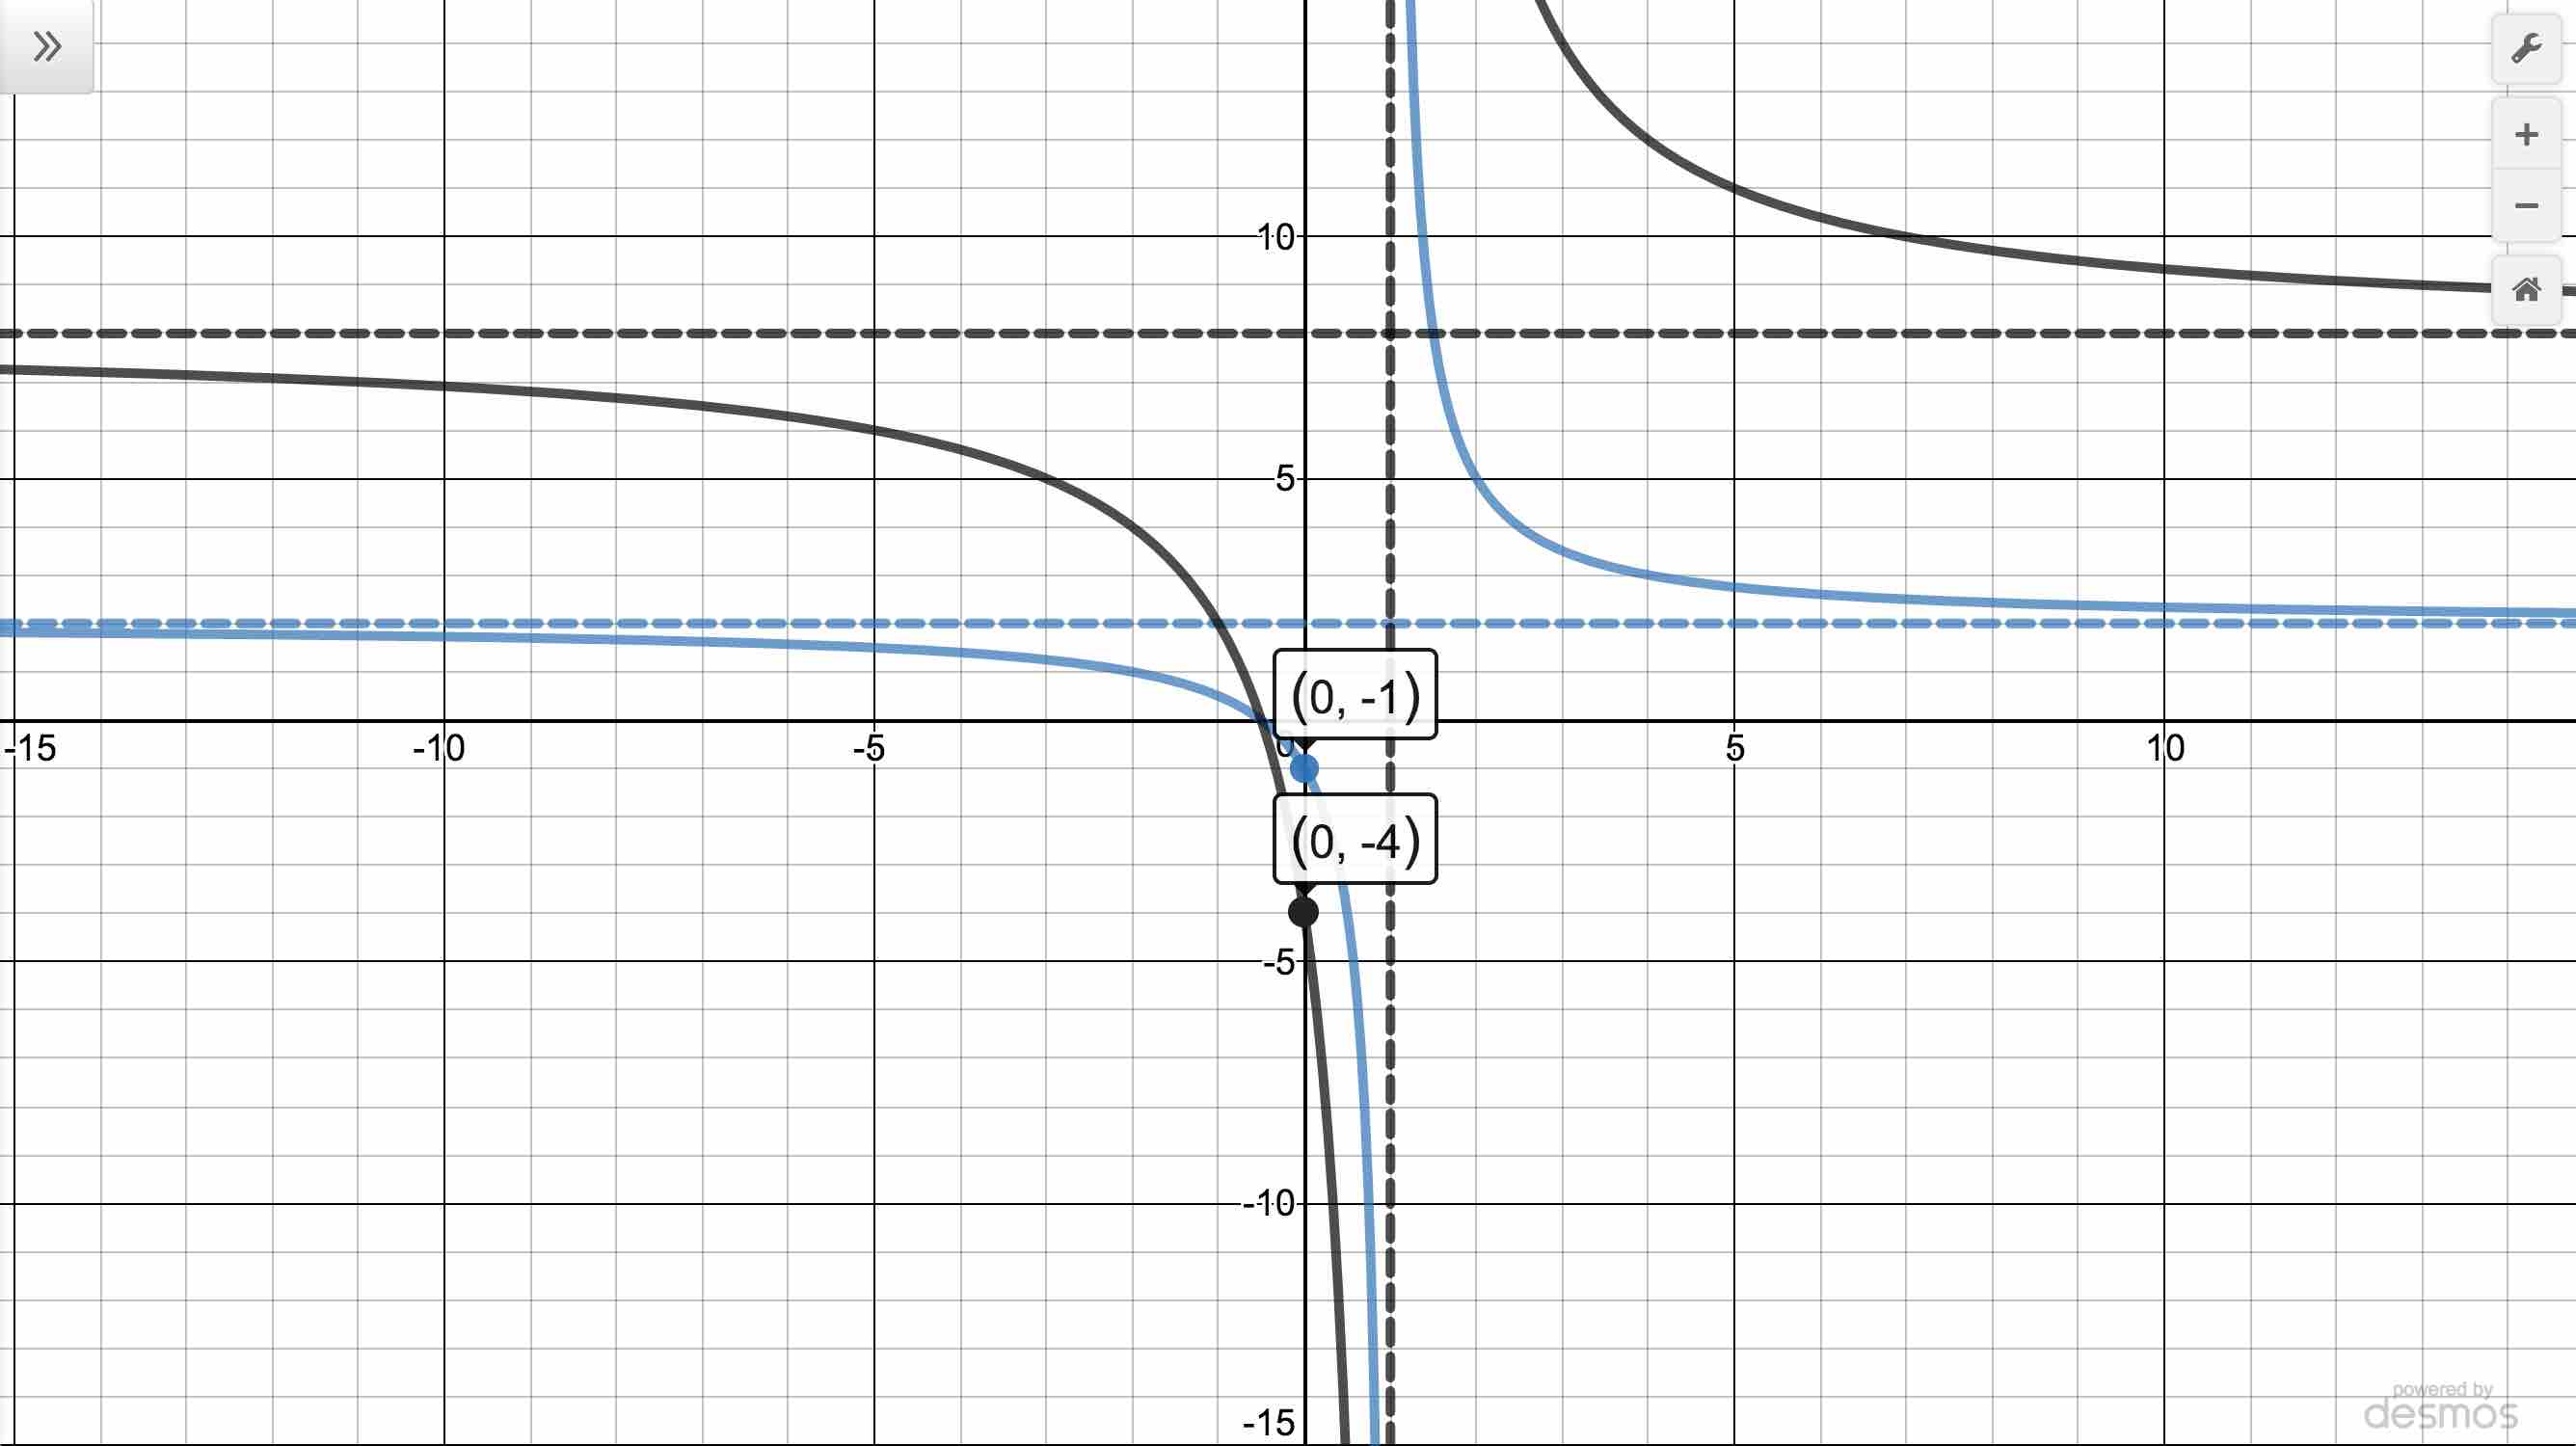
\includegraphics[width=3in]{./TransformationsGraphics/TransformationsEx03a.jpg} & 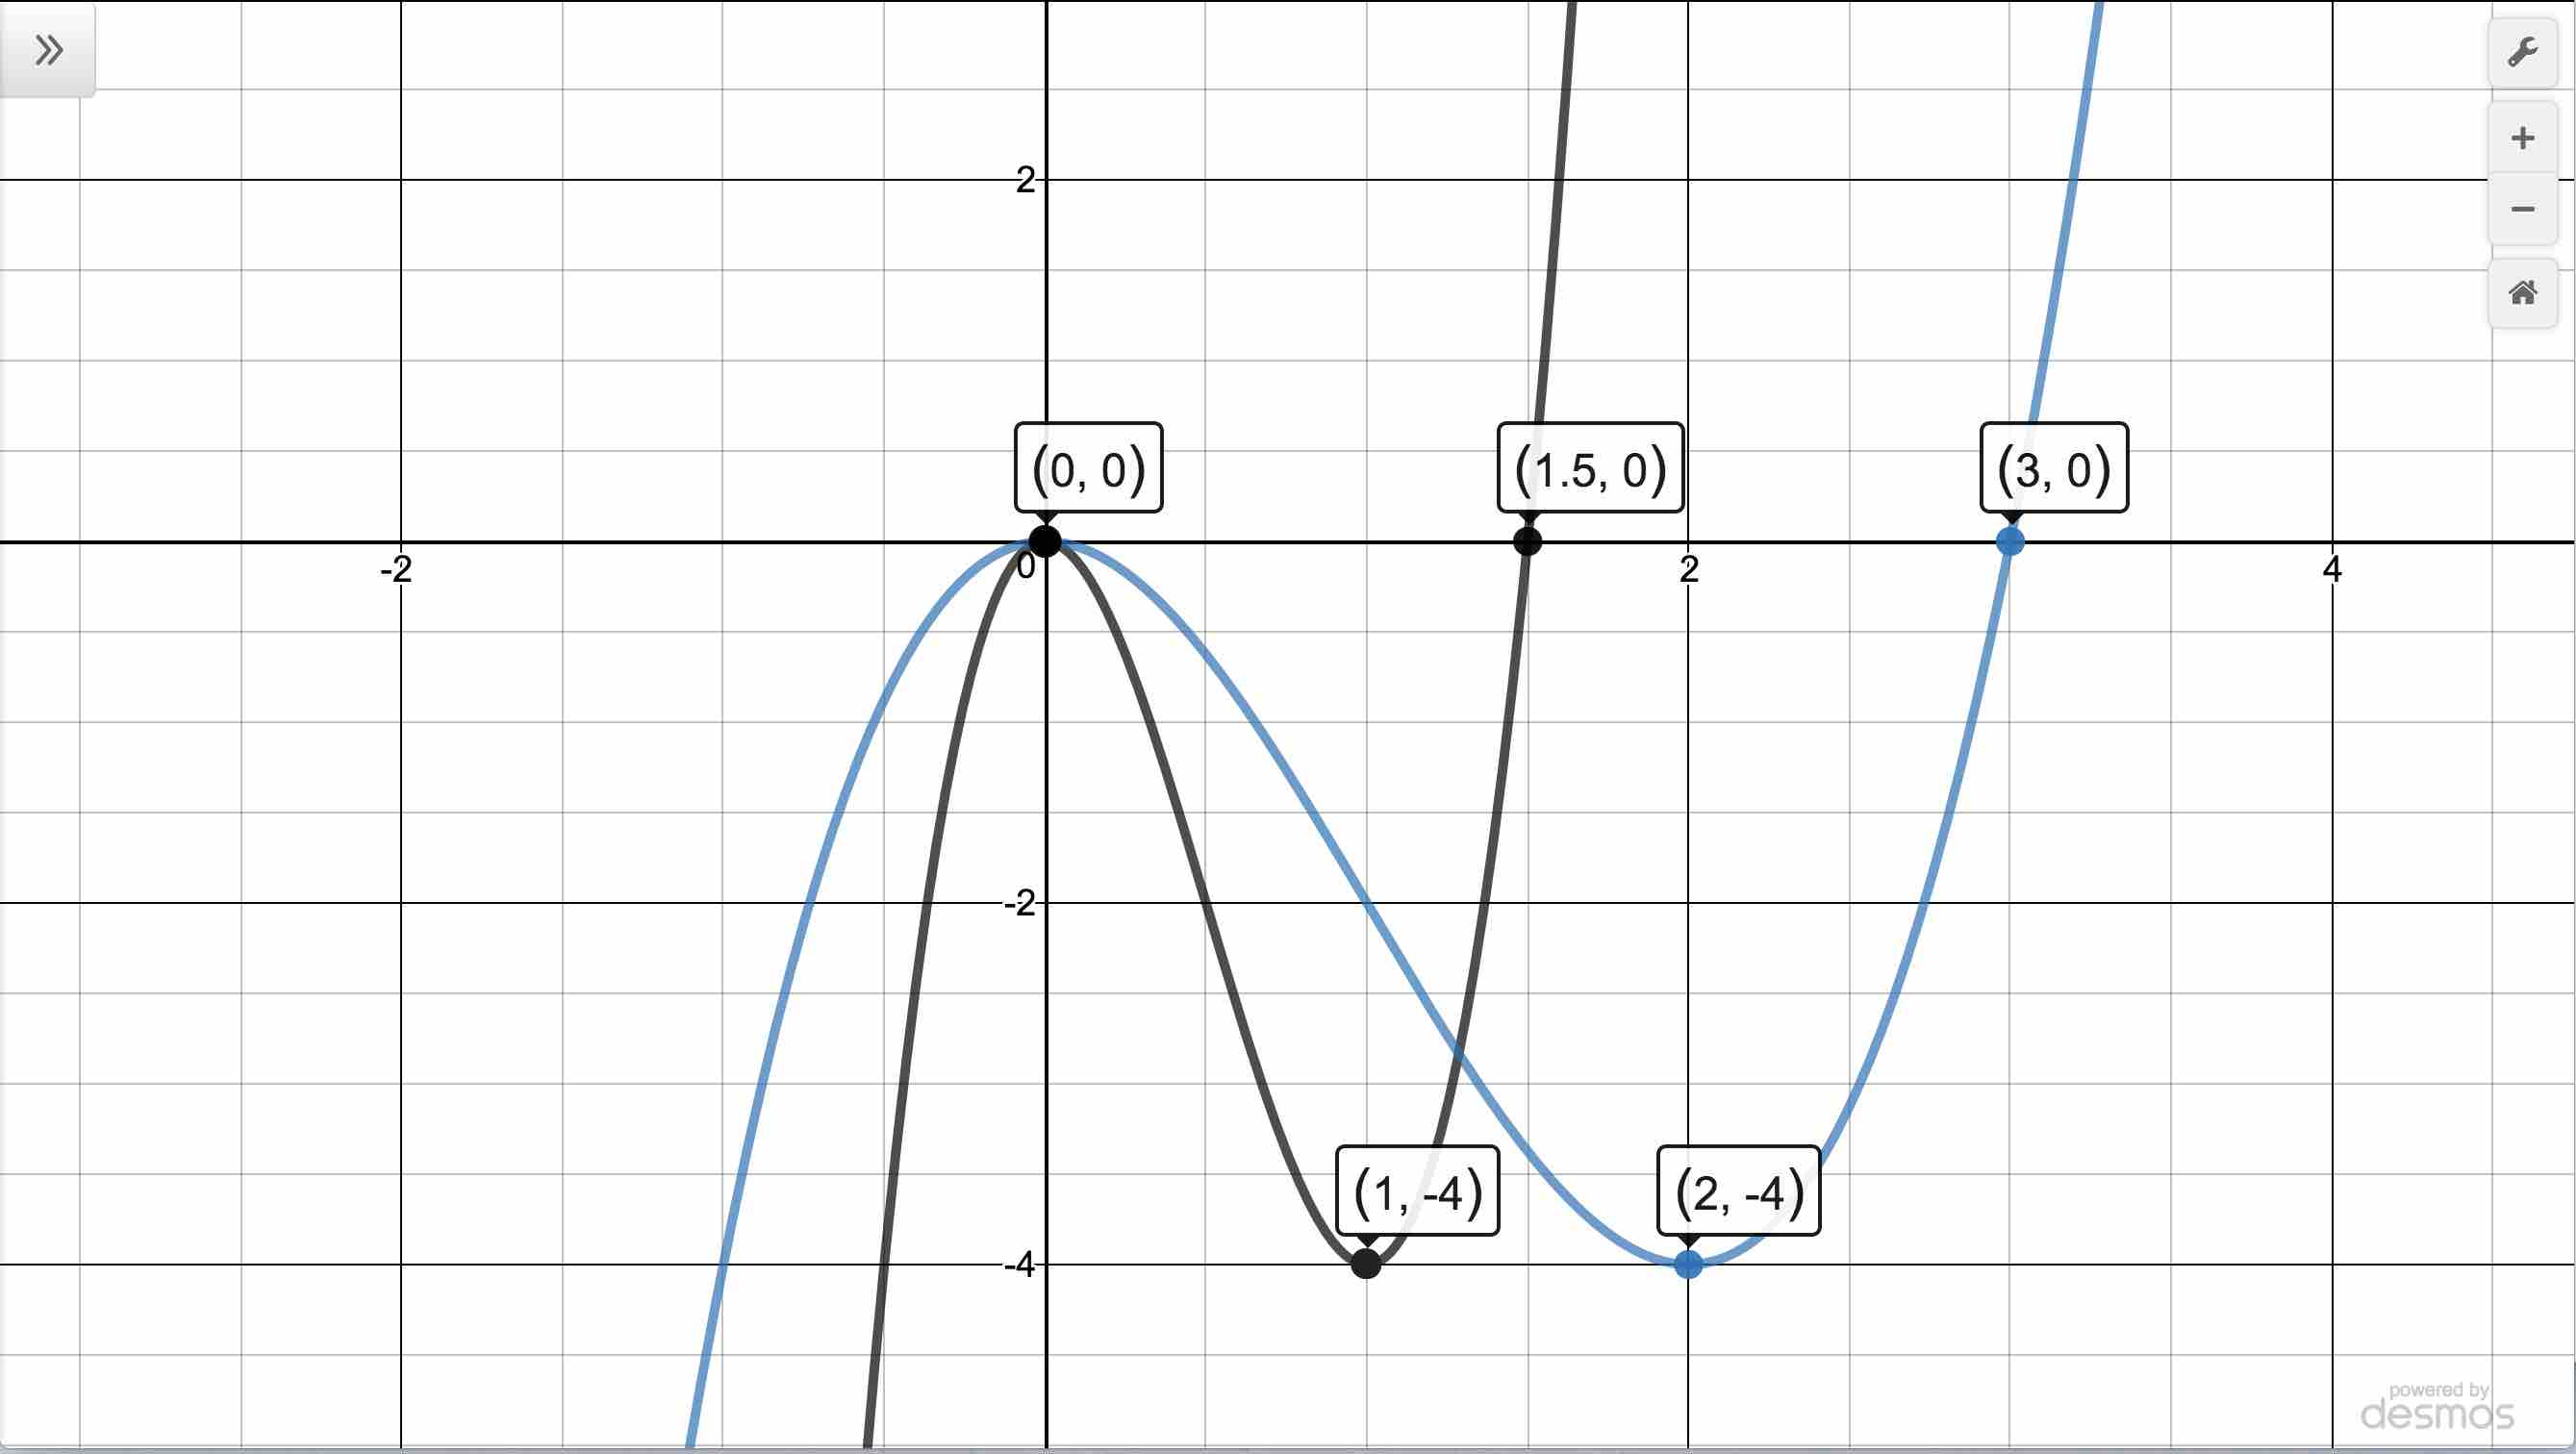
\includegraphics[width=3in]{./TransformationsGraphics/TransformationsEx03b.jpg} \\

{ \scriptsize $y=g(t) = \frac{2t+1}{t-1}$ (lighter color)  and $y=4g(t)=\dfrac{8t+4}{t-1}$}  &  {\scriptsize $y =  h(s) = s^3-3s^2$ (lighter color) and $y = H(s) = 8s^3 - 12s^2$} \\

\end{tabular}

\end{center} 
 
\item  

 
 \begin{enumerate}
 
 \item We first rewrite the expression for $F(x) = \frac{1-f(x)}{2} = -\frac{1}{2}f(x) + \frac{1}{2}$ in order to use the theorems available to us.  Note we have two modifications to the formula of $f(x)$ which correspond to three transformations.  
 
 \smallskip
 
 Multiplying $f(x)$ by $-\frac{1}{2}$ indicates a vertical compression by a factor of $2$ along with a reflection about the $x$-axis.  Adding $\frac{1}{2}$ indicates a vertical shift up $\frac{1}{2}$ units.  
 
 \smallskip
 
 As always the question is which to do first.  Once again, we look to algebra for the answer.  Picking the point $(1,0)$  on the graph of $f(x)$, we know $f(1) = 0$.  To see which point this corresponds to on the graph of $y=F(x)$, we find  $F(1) = -\frac{1}{2}f(1)+\frac{1}{2} = -\frac{1}{2} (0) +\frac{1}{2} = 0 + \frac{1}{2} = \frac{1}{2}$.  
 
 \smallskip
 
 Hence, we first multiplied the $y$-value $0$ by $-\frac{1}{2}$.  As above, we can think of $-\frac{1}{2} = (-1) \frac{1}{2}$  so that multiplying by $-\frac{1}{2}$ amounts to a vertical compression by a factor of $2$ first, then the refection about the $x$-axis second.  Lastly, adding the $\frac{1}{2}$ is the vertical shift up $\frac{1}{2}$ unit.  
 
 \smallskip
 
Beginning with the vertical scaling by a factor of $\frac{1}{2}$, we use Theorem \ref{vscalings} to graph $y=\frac{1}{2} f(x)$ starting from $y=f(x)$ by multiplying each of the $y$-coordinates of each of the points on the graph of $y=f(x)$ by $\frac{1}{2}$.
  


\[ \begin{array}{ccc}

\begin{mfpic}[15]{-1}{6}{-3}{3}
\axes
\tlabel[cc](6,-0.5){\scriptsize $x$}
\tlabel[cc](0.5,3){\scriptsize $y$}
\xmarks{ 0, 1, 2, 3,4,5}
\ymarks{-2, -1, 0, 1, 2}
\tcaption{\scriptsize $y = f(x)$}
\tlpointsep{4pt}
\scriptsize
\tlabel[cc](1.25, -0.75){$(1,0)$}
\tlabel[cc](2, 2){$(2,1)$}
\tlabel[cc](4, 2.75){$(4,2)$}
\axislabels {x}{{$2$} 2,{$3$} 3,{$4$} 4,{$5$} 5}
\axislabels {y}{{$-2$} -2,{$-1$} -1,{$1$} 1, {$2$} 2}
\normalsize
\penwd{1.25pt}
\arrow \reverse \arrow \parafcn{-2.5, 2.5, 0.1}{(2**t,t)}
\point[4pt]{(1,0), (2,1), (4,2)}
\end{mfpic}


&

\stackrel{\stackrel{\mbox{\scriptsize vertical scaling by a factor of $\frac{1}{2}$ }}{\xrightarrow{\hspace{1.7in}}}}{\mbox{ \scriptsize multiply each $y$-coordinate by $\frac{1}{2}$}} 

&

\begin{mfpic}[15]{-1}{6}{-3}{3}
\axes
\tlabel[cc](6,-0.5){\scriptsize $x$}
\tlabel[cc](0.5,3){\scriptsize $y$}
\xmarks{ 0, 1, 2, 3,4,5}
\ymarks{-2, -1, 0, 1, 2}
\tcaption{\scriptsize $y = \frac{1}{2}f(x)$}
\tlpointsep{4pt}
\scriptsize
\tlabel[cc](1, -0.75){$(1,0)$}
\tlabel[cc](2, 1.25){$\left(2, \frac{1}{2} \right)$}
\tlabel[cc](4, 1.5){$(4,1)$}
\axislabels {x}{{$2$} 2,{$3$} 3,{$4$} 4,{$5$} 5}
\axislabels {y}{{$-2$} -2,{$-1$} -1,{$1$} 1, {$2$} 2}
\normalsize
\penwd{1.25pt}
\arrow \reverse \arrow \parafcn{-3, 2.55, 0.1}{(2**t,t/2)}
\point[4pt]{(1,0), (2,0.5), (4,1)}
\end{mfpic} \\
 
\end{array} \]

Next, we reflect the graph of $y = \frac{1}{2} f(x)$ across the $x$-axis to produce the graph of $y=-\frac{1}{2} f(x)$ by multiplying each of the $y$-coordinates of the points on the graph of $y=\frac{1}{2} f(x)$ by $-1$:



\[ \begin{array}{ccc}

\begin{mfpic}[15]{-1}{6}{-3}{3}
\axes
\tlabel[cc](6,-0.5){\scriptsize $x$}
\tlabel[cc](0.5,3){\scriptsize $y$}
\xmarks{ 0, 1, 2, 3,4,5}
\ymarks{-2, -1, 0, 1, 2}
\tcaption{\scriptsize $y = \frac{1}{2}f(x)$}
\tlpointsep{4pt}
\scriptsize
\tlabel[cc](1, -0.75){$(1,0)$}
\tlabel[cc](2, 1.25){$\left(2, \frac{1}{2} \right)$}
\tlabel[cc](4, 1.5){$(4,1)$}
\axislabels {x}{{$2$} 2,{$3$} 3,{$4$} 4,{$5$} 5}
\axislabels {y}{{$-2$} -2,{$-1$} -1,{$1$} 1, {$2$} 2}
\normalsize
\penwd{1.25pt}
\arrow \reverse \arrow \parafcn{-3, 2.55, 0.1}{(2**t,t/2)}
\point[4pt]{(1,0), (2,0.5), (4,1)}
\end{mfpic}

&

\stackrel{\stackrel{\mbox{\scriptsize reflect about the $x$-axis }}{\xrightarrow{\hspace{1.7in}}}}{\mbox{ \scriptsize multiply each $y$-coordinate by $-1$}} 

&

\begin{mfpic}[15]{-1}{6}{-3}{3}
\axes
\tlabel[cc](6,-0.5){\scriptsize $x$}
\tlabel[cc](0.5,3){\scriptsize $y$}
\xmarks{ 0, 1, 2, 3,4,5}
\ymarks{-2, -1, 0, 1, 2}
\tcaption{\scriptsize $y = -\frac{1}{2}f(x)$}
\tlpointsep{4pt}
\scriptsize
\tlabel[cc](1.25, 0.5){$(1,0)$}
\tlabel[cc](2, -1.25){$\left(2, -\frac{1}{2} \right)$}
\tlabel[cc](4, -1.5){$(4,-1)$}
\axislabels {x}{{$3$} 3,{$4$} 4,{$5$} 5}
\axislabels {y}{{$-2$} -2,{$-1$} -1,{$1$} 1, {$2$} 2}
\normalsize
\penwd{1.25pt}
\arrow \reverse \arrow \parafcn{-3, 2.55, 0.1}{(2**t,-t/2)}
\point[4pt]{(1,0), (2,-0.5), (4,-1)}
\end{mfpic} \\
 
\end{array} \]

Finally, we shift the graph of $y = -\frac{1}{2} f(x)$ vertically up $\frac{1}{2}$ unit by adding $\frac{1}{2}$ to each of the $y$-coordinates of each of the points to obtain the graph of $y = -\frac{1}{2}f(x)+\frac{1}{2} = F(x)$.
 
 
\[ \begin{array}{ccc}

\begin{mfpic}[15]{-1}{6}{-3}{3}
\axes
\tlabel[cc](6,-0.5){\scriptsize $x$}
\tlabel[cc](0.5,3){\scriptsize $y$}
\xmarks{ 0, 1, 2, 3,4,5}
\ymarks{-2, -1, 0, 1, 2}
\tcaption{\scriptsize $y = -\frac{1}{2}f(x)$}
\tlpointsep{4pt}
\scriptsize
\tlabel[cc](1.25, 0.5){$(1,0)$}
\tlabel[cc](2, -1.25){$\left(2, -\frac{1}{2} \right)$}
\tlabel[cc](4, -1.5){$(4,-1)$}
\axislabels {x}{{$3$} 3,{$4$} 4,{$5$} 5}
\axislabels {y}{{$-2$} -2,{$-1$} -1,{$1$} 1, {$2$} 2}
\normalsize
\penwd{1.25pt}
\arrow \reverse \arrow \parafcn{-3, 2.55, 0.1}{(2**t,-t/2)}
\point[4pt]{(1,0), (2,-0.5), (4,-1)}
\end{mfpic} 
 


&

\stackrel{\stackrel{\mbox{\scriptsize shift up $\frac{1}{2}$ unit }}{\xrightarrow{\hspace{1.7in}}}}{\mbox{ \scriptsize add $\frac{1}{2}$ to each $y$-coordinate}} 

&

\begin{mfpic}[15]{-1}{6}{-3}{3}
\axes
\tlabel[cc](6,-0.5){\scriptsize $x$}
\tlabel[cc](0.5,3){\scriptsize $y$}
\xmarks{ 0, 1, 2, 3,4,5}
\ymarks{-2, -1, 0, 1, 2}
\tcaption{\scriptsize $y = -\frac{1}{2}f(x)+\frac{1}{2} = F(x)$}
\tlpointsep{4pt}
\scriptsize
\tlabel[cc](1.5, 1){$\left(1,\frac{1}{2} \right)$}
\tlabel[cc](2, -0.5){$(2,0)$}
\tlabel[cc](4, -1.25){$\left(4,-\frac{1}{2} \right)$}
\axislabels {x}{{$1$} 1,{$5$} 5}
\axislabels {y}{{$-2$} -2,{$-1$} -1,{$1$} 1, {$2$} 2}
\normalsize
\penwd{1.25pt}
\arrow \reverse \arrow \parafcn{-3, 2.55, 0.1}{(2**t,-t/2+0.5)}
\point[4pt]{(1,0.5), (2,0), (4,-0.5)}
\end{mfpic} \\
 
\end{array} \]

Note that as with horizontal scalings and reflections about the $y$-axis, the order of vertical scalings and reflections across the $x$-axis is interchangeable.  Had we decided to think of the factor $-\frac{1}{2} = \frac{1}{2} \cdot (-1)$, we could have just as well started with the graph of $y=f(x)$ and produced the graph of $y=-f(x)$ first:

\[ \begin{array}{ccc}

\begin{mfpic}[15]{-1}{6}{-3}{3}
\axes
\tlabel[cc](6,-0.5){\scriptsize $x$}
\tlabel[cc](0.5,3){\scriptsize $y$}
\xmarks{ 0, 1, 2, 3,4,5}
\ymarks{-2, -1, 0, 1, 2}
\tcaption{\scriptsize $y = f(x)$}
\tlpointsep{4pt}
\scriptsize
\tlabel[cc](1.25, -0.75){$(1,0)$}
\tlabel[cc](2, 2){$(2,1)$}
\tlabel[cc](4, 2.75){$(4,2)$}
\axislabels {x}{{$2$} 2,{$3$} 3,{$4$} 4,{$5$} 5}
\axislabels {y}{{$-2$} -2,{$-1$} -1,{$1$} 1, {$2$} 2}
\normalsize
\penwd{1.25pt}
\arrow \reverse \arrow \parafcn{-2.5, 2.5, 0.1}{(2**t,t)}
\point[4pt]{(1,0), (2,1), (4,2)}
\end{mfpic}


&

\stackrel{\stackrel{\mbox{\scriptsize reflect across the $x$-axis }}{\xrightarrow{\hspace{1.7in}}}}{\mbox{ \scriptsize multiply each $y$-coordinate by $-1$}} 

&

\begin{mfpic}[15]{-1}{6}{-3}{3}
\axes
\tlabel[cc](6,-0.5){\scriptsize $x$}
\tlabel[cc](0.5,3){\scriptsize $y$}
\xmarks{ 0, 1, 2, 3,4,5}
\ymarks{-2, -1, 0, 1, 2}
\tcaption{\scriptsize $y = -f(x)$}
\tlpointsep{4pt}
\scriptsize
\tlabel[cc](1.5, 0.5){$(1,0)$}
\tlabel[cc](2, -1.75){$(2,-1)$}
\tlabel[cc](4, -2.75){$(4,-2)$}
\axislabels {x}{{$2$} 2,{$3$} 3,{$4$} 4,{$5$} 5}
\axislabels {y}{{$-2$} -2,{$-1$} -1,{$1$} 1, {$2$} 2}
\normalsize
\penwd{1.25pt}
\arrow \reverse \arrow \parafcn{-2.5, 2.5, 0.1}{(2**t,-t)}
\point[4pt]{(1,0), (2,-1), (4,-2)}
\end{mfpic} \\
 
\end{array} \]

Next, we vertically scale the graph of $y=-f(x)$  by multiplying each of the $y$-coordinates of each of the points on the graph of $y=-f(x)$ by $\frac{1}{2}$ to obtain the graph of $y = -\frac{1}{2} f(x)$:

 
 
 \[ \begin{array}{ccc}

\begin{mfpic}[15]{-1}{6}{-3}{3}
\axes
\tlabel[cc](6,-0.5){\scriptsize $x$}
\tlabel[cc](0.5,3){\scriptsize $y$}
\xmarks{ 0, 1, 2, 3,4,5}
\ymarks{-2, -1, 0, 1, 2}
\tcaption{\scriptsize $y = -f(x)$}
\tlpointsep{4pt}
\scriptsize
\tlabel[cc](1, -1){$(1,0)$}
\tlabel[cc](2, -2){$(2,-1)$}
\tlabel[cc](4, -2.75){$(4,-2)$}
\axislabels {x}{{$2$} 2,{$3$} 3,{$4$} 4,{$5$} 5}
\axislabels {y}{{$-2$} -2,{$-1$} -1,{$1$} 1, {$2$} 2}
\normalsize
\penwd{1.25pt}
\arrow \reverse \arrow \parafcn{-2.5, 2.5, 0.1}{(2**t,-t)}
\point[4pt]{(1,0), (2,-1), (4,-2)}
\end{mfpic}

&

\stackrel{\stackrel{\mbox{\scriptsize vertical scaling by a factor of $\frac{1}{2}$ }}{\xrightarrow{\hspace{1.7in}}}}{\mbox{ \scriptsize multiply each $y$-coordinate by $\frac{1}{2}$}} 

&

\begin{mfpic}[15]{-1}{6}{-3}{3}
\axes
\tlabel[cc](6,-0.5){\scriptsize $x$}
\tlabel[cc](0.5,3){\scriptsize $y$}
\xmarks{ 0, 1, 2, 3,4,5}
\ymarks{-2, -1, 0, 1, 2}
\tcaption{\scriptsize $y = -\frac{1}{2}f(x)$}
\tlpointsep{4pt}
\scriptsize
\tlabel[cc](1.25, 0.5){$(1,0)$}
\tlabel[cc](2, -1.25){$\left(2, -\frac{1}{2} \right)$}
\tlabel[cc](4, -1.5){$(4,-1)$}
\axislabels {x}{{$3$} 3,{$4$} 4,{$5$} 5}
\axislabels {y}{{$-2$} -2,{$-1$} -1,{$1$} 1, {$2$} 2}
\normalsize
\penwd{1.25pt}
\arrow \reverse \arrow \parafcn{-3, 2.55, 0.1}{(2**t,-t/2)}
\point[4pt]{(1,0), (2,-0.5), (4,-1)}
\end{mfpic} \\
 
\end{array} \]


Notice we've reached the same graph of $y=-\frac{1}{2} f(x)$ that we had before, and, hence we arrive at the same final answer as before:

\[ \begin{array}{ccc}

\begin{mfpic}[15]{-1}{6}{-3}{3}
\axes
\tlabel[cc](6,-0.5){\scriptsize $x$}
\tlabel[cc](0.5,3){\scriptsize $y$}
\xmarks{ 0, 1, 2, 3,4,5}
\ymarks{-2, -1, 0, 1, 2}
\tcaption{\scriptsize $y = -\frac{1}{2}f(x)$}
\tlpointsep{4pt}
\scriptsize
\tlabel[cc](1.25, 0.5){$(1,0)$}
\tlabel[cc](2, -1.25){$\left(2, -\frac{1}{2} \right)$}
\tlabel[cc](4, -1.5){$(4,-1)$}
\axislabels {x}{{$3$} 3,{$4$} 4,{$5$} 5}
\axislabels {y}{{$-2$} -2,{$-1$} -1,{$1$} 1, {$2$} 2}
\normalsize
\penwd{1.25pt}
\arrow \reverse \arrow \parafcn{-3, 2.55, 0.1}{(2**t,-t/2)}
\point[4pt]{(1,0), (2,-0.5), (4,-1)}
\end{mfpic} 
 


&

\stackrel{\stackrel{\mbox{\scriptsize shift up $\frac{1}{2}$ unit }}{\xrightarrow{\hspace{1.7in}}}}{\mbox{ \scriptsize add $\frac{1}{2}$ to each $y$-coordinate}} 

&

\begin{mfpic}[15]{-1}{6}{-3}{3}
\axes
\tlabel[cc](6,-0.5){\scriptsize $x$}
\tlabel[cc](0.5,3){\scriptsize $y$}
\xmarks{ 0, 1, 2, 3,4,5}
\ymarks{-2, -1, 0, 1, 2}
\tcaption{\scriptsize $y = -\frac{1}{2}f(x)+\frac{1}{2} = F(x)$}
\tlpointsep{4pt}
\scriptsize
\tlabel[cc](1.5, 1){$\left(1,\frac{1}{2} \right)$}
\tlabel[cc](2, -0.5){$(2,0)$}
\tlabel[cc](4, -1.25){$\left(4,-\frac{1}{2} \right)$}
\axislabels {x}{{$1$} 1,{$5$} 5}
\axislabels {y}{{$-2$} -2,{$-1$} -1,{$1$} 1, {$2$} 2}
\normalsize
\penwd{1.25pt}
\arrow \reverse \arrow \parafcn{-3, 2.55, 0.1}{(2**t,-t/2+0.5)}
\point[4pt]{(1,0.5), (2,0), (4,-0.5)}
\end{mfpic} \\
 
\end{array} \]

We check our answer as we have so many times before.  We start with the point $\left(1, \frac{1}{2}\right)$ and substitute $x=1$ into $y=\frac{1-f(x)}{2}$ to get $y=\frac{1-f(1)}{2}$.  From the graph of $f$, we know $f(1) = 0$, so we get $y=\frac{1-f(1)}{2} = \frac{1-0}{2} = \frac{1}{2}$.  This proves $\left(1, \frac{1}{2}\right)$ is on the graph of $y=\frac{1-f(x)}{2}$.  We invite the reader to check the remaining points.


Note that in the preceding example, since none of the transformations included adjusting the $x$-coordinates of points, the vertical asymptote, $x=0$ remained in place.

 
  \item  As with the previous example, we first rewrite $F(x)= f\left( \frac{1-x}{2} \right) = F\left( -\frac{1}{2}x + \frac{1}{2} \right)$.  Here again, we have two modifications to the formula $f(x)$, the $-\frac{1}{2}$ multiple indicating a horizontal scaling and a reflection across the $y$-axis and a horizontal shift. 
  
  \smallskip
  
   Based on our experience from previous examples, we do the horizontal shift first, with the order of the scaling and reflection more or less irrelevant.   
  
  \smallskip
  
  To  produce the graph of $y = f\left(x+\frac{1}{2}\right)$ we subtract $\frac{1}{2}$ from each of the $x$-coordinates of each of the points on the graph of $y=f(x)$.  This moves the graph to the left $\frac{1}{2}$ unit, including the vertical asymptote $x=0$ which moves to $x = -\frac{1}{2}$.
  
\[ \begin{array}{ccc}

\begin{mfpic}[15]{-1}{6}{-3}{3}
\axes
\tlabel[cc](6,-0.5){\scriptsize $x$}
\tlabel[cc](0.5,3){\scriptsize $y$}
\xmarks{ 0, 1, 2, 3,4,5}
\ymarks{-2, -1, 0, 1, 2}
\tcaption{\scriptsize $y = f(x)$}
\tlpointsep{4pt}
\scriptsize
\tlabel[cc](1.25, -0.75){$(1,0)$}
\tlabel[cc](2, 2){$(2,1)$}
\tlabel[cc](4, 2.75){$(4,2)$}
\axislabels {x}{{$2$} 2,{$3$} 3,{$4$} 4,{$5$} 5}
\axislabels {y}{{$-2$} -2,{$-1$} -1,{$1$} 1, {$2$} 2}
\normalsize
\penwd{1.25pt}
\arrow \reverse \arrow \parafcn{-2.5, 2.5, 0.1}{(2**t,t)}
\point[4pt]{(1,0), (2,1), (4,2)}
\end{mfpic}


&

\stackrel{\stackrel{\mbox{\scriptsize shift left $\frac{1}{2}$ unit }}{\xrightarrow{\hspace{1.7in}}}}{\mbox{ \scriptsize subtract $\frac{1}{2}$ from each $x$-coordinate}} 

&

\begin{mfpic}[15]{-2}{5}{-3}{3}
\axes
\tlabel[cc](5,-0.5){\scriptsize $x$}
\tlabel[cc](0.5,3){\scriptsize $y$}
\xmarks{ -1, 0, 1, 2, 3,4}
\ymarks{-2, -1, 0, 1, 2}
\tcaption{\scriptsize $y = f\left(x + \frac{1}{2} \right)$}
\tlpointsep{4pt}
\scriptsize
\tlabel[cc](1, -0.75){$\left( \frac{1}{2} ,0 \right)$}
\tlabel[cc](1.25, 1.75){$\left( \frac{3}{2} ,1\right)$}
\tlabel[cc](3.25, 2.5){$\left(\frac{7}{2},2 \right)$}
\axislabels {x}{{$-1 \hspace{7pt}$} -1, {$2$} 2,{$3$} 3,{$4$} 4}
\axislabels {y}{{$1$} 1,{ $2$} 2}
\normalsize
\dashed \polyline{(-0.5, -3), (-0.5, 3)}
\tlabel[cc](-1.5, -2.5){\scriptsize $x=-\frac{1}{2}$}
\penwd{1.25pt}
\arrow \reverse \arrow \parafcn{-2.5, 2.5, 0.1}{((2**t) - 0.5,t)}
\point[4pt]{(0.5,0), (1.5,1), (3.5,2)}
\end{mfpic} \\
 
\end{array} \]


Next, we graph $y = f\left(\frac{1}{2}x + \frac{1}{2} \right)$ starting with $y = f\left(x+\frac{1}{2}\right)$ by horizontally expanding the graph by a factor of $2$.  That is, we multiply each $x$-coordinates on the graph of $y = f\left(x+\frac{1}{2}\right)$  by $2$, including the vertical asymptote, $x  =-\frac{1}{2}$ which moves to $x = 2 \left(-\frac{1}{2} \right) = -1$.


\[ \begin{array}{ccc}

\begin{mfpic}[15]{-2}{5}{-3}{3}
\axes
\tlabel[cc](5,-0.5){\scriptsize $x$}
\tlabel[cc](0.5,3){\scriptsize $y$}
\xmarks{ -1, 0, 1, 2, 3,4}
\ymarks{-2, -1, 0, 1, 2}
\tcaption{\scriptsize $y = f\left(x + \frac{1}{2} \right)$}
\tlpointsep{4pt}
\scriptsize
\tlabel[cc](1, -0.75){$\left( \frac{1}{2} ,0 \right)$}
\tlabel[cc](1.25, 1.75){$\left( \frac{3}{2} ,1\right)$}
\tlabel[cc](3.25, 2.5){$\left(\frac{7}{2},2 \right)$}
\axislabels {x}{{$-1 \hspace{7pt}$} -1, {$2$} 2,{$3$} 3,{$4$} 4}
\axislabels {y}{{$1$} 1,{ $2$} 2}
\normalsize
\dashed \polyline{(-0.5, -3), (-0.5, 3)}
\tlabel[cc](-1.5, -2.5){\scriptsize $x=-\frac{1}{2}$}
\penwd{1.25pt}
\arrow \reverse \arrow \parafcn{-2.5, 2.5, 0.1}{((2**t) - 0.5,t)}
\point[4pt]{(0.5,0), (1.5,1), (3.5,2)}
\end{mfpic}


&

\stackrel{\stackrel{\mbox{\scriptsize horizontal scaling by a factor of $2$ }}{\xrightarrow{\hspace{1.7in}}}}{\mbox{ \scriptsize multiply eac $x$-coordinate by $2$}} 

&

\begin{mfpic}[11][15]{-2}{10}{-3}{3}
\axes
\tlabel[cc](10,-0.5){\scriptsize $x$}
\tlabel[cc](0.5,3){\scriptsize $y$}
\xmarks{-2, -1, 0, 1, 2, 3,4,5,6,7,8,9}
\ymarks{-2, -1, 0, 1, 2}
\tcaption{\scriptsize $y = f\left(\frac{1}{2}x + \frac{1}{2} \right)$}
\tlpointsep{4pt}
\scriptsize
\tlabel[cc](0.75, 0.5){$(1,0)$}
\tlabel[cc](3, 1.5){$(3,1)$}
\tlabel[cc](7, 2.5){$(7,2)$}
\axislabels {x}{{$-2 \hspace{7pt}$} -2, ,{$1$} 1, {$2$} 2,{$3$} 3,{$4$} 4,{$5$} 5,{$6$} 6,{$7$} 7,{$8$} 8,{$9$} 9}
\axislabels {y}{{$1$} 1,{ $2$} 2}
\normalsize
\dashed \polyline{(-1, -3), (-1, 3)}
\tlabel[cc](-2.5, -2.5){\scriptsize $x=-1$}
\penwd{1.25pt}
\arrow \reverse \arrow \parafcn{-2.5, 2.4, 0.1}{(   2*((2**t) - 0.5),t)}
\point[4pt]{(1,0), (3,1), (7,2)}
\end{mfpic} \\
 
\end{array} \]

Finally, we reflect the graph of $y = f\left(\frac{1}{2}x + \frac{1}{2} \right)$ about the $y$-axis to graph $y = f\left(-\frac{1}{2}x + \frac{1}{2} \right)$. We accomplish this by multiplying each of the $x$-coordinates of each of the points on the graph of  $y = f\left(\frac{1}{2}x + \frac{1}{2} \right)$ by $-1$.  This includes the vertical asymptote which is moved to $x = (-1)(-1) = 1$.


 \[ \begin{array}{ccc}

\begin{mfpic}[11][15]{-2}{10}{-3}{3}
\axes
\tlabel[cc](10,-0.5){\scriptsize $x$}
\tlabel[cc](0.5,3){\scriptsize $y$}
\xmarks{-2, -1, 0, 1, 2, 3,4,5,6,7,8,9}
\ymarks{-2, -1, 0, 1, 2}
\tcaption{\scriptsize $y = f\left(\frac{1}{2}x + \frac{1}{2} \right)$}
\tlpointsep{4pt}
\scriptsize
\tlabel[cc](0.75, 0.5){$(1,0)$}
\tlabel[cc](3, 1.5){$(3,1)$}
\tlabel[cc](7, 2.5){$(7,2)$}
\axislabels {x}{{$-2 \hspace{7pt}$} -2, ,{$1$} 1, {$2$} 2,{$3$} 3,{$4$} 4,{$5$} 5,{$6$} 6,{$7$} 7,{$8$} 8,{$9$} 9}
\axislabels {y}{{$1$} 1,{ $2$} 2}
\normalsize
\dashed \polyline{(-1, -3), (-1, 3)}
\tlabel[cc](-2.5, -2.5){\scriptsize $x=-1$}
\penwd{1.25pt}
\arrow \reverse \arrow \parafcn{-2.5, 2.4, 0.1}{(   2*((2**t) - 0.5),t)}
\point[4pt]{(1,0), (3,1), (7,2)}
\end{mfpic}


&

\stackrel{\stackrel{\mbox{\scriptsize horizontal scaling by a factor of $2$ }}{\xrightarrow{\hspace{1.7in}}}}{\mbox{ \scriptsize multiply each $x$-coordinate by $2$}} 

&

\begin{mfpic}[11][15]{-10}{2}{-3}{3}
\axes
\tlabel[cc](2,-0.5){\scriptsize $x$}
\tlabel[cc](0.5,3){\scriptsize $y$}
\xmarks{1, 0, -1, -2, -3,-4,-5,-6,-7,-8,-9}
\ymarks{-2, -1, 0, 1, 2}
\tcaption{\scriptsize $y = f\left(-\frac{1}{2}x + \frac{1}{2} \right)$}
\tlpointsep{4pt}
\scriptsize
\tlabel[cc](-1.5, -0.75){$(-1,0)$}
\tlabel[cc](-2.75, 1.5){$(-3,1)$}
\tlabel[cc](-7, 2.5){$(-7,2)$}
\axislabels {x}{  {$-3 \hspace{7pt}$} -3,  {$-5 \hspace{7pt}$} -5, {$-7 \hspace{7pt}$} -7, {$-9 \hspace{7pt}$} -9}
\axislabels {y}{{$1$} 1,{ $2$} 2}
\normalsize
\dashed \polyline{(1, -3), (1, 3)}
\tlabel[cc](2.5, -2.5){\scriptsize $x=1$}
\penwd{1.25pt}
\arrow \reverse \arrow \parafcn{-2.5, 2.4, 0.1}{(  0 - (2* ( (2**t) - 0.5)  ),  t  )}


\point[4pt]{(-1,0), (-3,1), (-7,2)}
\end{mfpic} \\
 
\end{array} \]

To check our answer, we begin with the point $(-1,0)$ and substitute $x=-1$ into $y = f\left( \frac{1-x}{2} \right)$.  We get $y = f\left( \frac{1-(-1)}{2} \right) = f\left( \frac{2}{2} \right) = f(1)$.  From the graph of $f$, we know $f(1) = 0$, hence we have $y = f(1) = 0$, proving $(-1,0)$ is on the graph of $y = f\left( \frac{1-x}{2}\right)$.  The reader is encouraged to check the remaining points.


As mentioned previously, instead of doing the horizontal scaling first, then the reflection, we could have done the reflection first, then the scaling.  We leave this to the reader to check.

 \end{enumerate}

 
 \item To write $g(x)$ in terms of $f(x)$, we assume we can find real numbers $a$, $b$, $h$, and $k$ and choose signs $\pm$ so that $g(x) = \pm a f(\pm b x - h)+k$.   
 
 \smallskip
 
 The most notable change we see is the vertical asymptote $x=0$ has moved to $x=2$.  Moreover, instead of the graph increasing off to the right, it is decreasing coming in from the left.  This suggests a horizontal shift of $2$ units as well as a reflection across the $y$-axis.  
 
 \smallskip
 
 Since we always shift first then reflect, we have a shift \textit{left} of $2$ units followed by a reflection about the $y$-axis.  In other words, $g(x) = \pm a f(-x+2) + k$.  
 
 \smallskip
 
 Comparing $y$-values, the $y$-values on the graph of $g$ appear to be exactly twice the corresponding values on the graph of $f$, indicating a vertical stretch by a factor of $2$.  Hence, we get $g(x) = 2 f(-x+2)$.  We leave it to the reader to check the graph of $y=2f(-x+2)$ matches the graph of $y=g(x)$.  
 
 \smallskip
 
To write $f(x)$ in terms of $g(x)$, we reverse the steps done in obtaining the graph of $g(x)$ from $f(x)$ in the reverse order.  

\smallskip

Since to get from the graph of $f$ to the graph of $g$, we: first, shifted left $2$ units; second reflected across the $y$-axis; third, vertically stretched by a factor of $2$, our first step in taking $g$ back to $f$ is to implement a vertical compression by a factor of $2$.  Hence, starting with the graph of $y=g(x)$, our first step results in the formula $y = \frac{1}{2} g(x)$. 

\smallskip

 Next, we need to undo the reflection abut the $y$-axis.  If the point $(a,b)$ is reflected about the $y$-axis, we obtain the point $(-a,b)$.  To return to the point $(a,b)$, we reflect $(-a,b)$ across the $y$-axis again: $(-(-a),b) = (a,b)$.  Hence, we take the graph of $y = \frac{1}{2} g(x)$ and reflect it across the $y$-axis to obtain $y = \frac{1}{2} g(-x)$.  
 
 \smallskip
 
 Our last step is to undo a horizontal shift to the left $2$ units.  The reverse of this process is shifting the graph to the \textit{right} two units, so we get $y = \frac{1}{2} g(-(x-2)) = \frac{1}{2} g(-x+2)$.\footnote{To see this better, let $F(x) = \frac{1}{2} g(-x)$.  Per Theorem \ref{hshifts}, the graph of  $F(x-2) = \frac{1}{2} g(-(x-2)) = \frac{1}{2} g(-x+2)$ is the same as the graph of $F$ but shifted $2$ units to the right.}  
 
 \smallskip
 
 We leave it to the reader to start with the graph of $y=g(x)$ and check the graph of $y =  \frac{1}{2} g(-x+2)$ matches the graph of $y = f(x)$. \qed

\end{enumerate}

\end{ex}

\subsection{Transformations in Sequence}
\label{TransformationsinSequence}


Now that we have studied  three basic classes of transformations:  shifts, reflections, and scalings, we present a result below which provides one algorithm to follow to transform the graph of $y=f(x)$ into the graph of $y=af(bx-h)+k$ without the need of using Theorems \ref{vshifts}, \ref{hshifts}, \ref{reflections}, \ref{vscalings} and \ref{hscalings} individually.  

\smallskip

Theorem \ref{transformationsthm} is the ultimate generalization of Theorems \ref{linearabsvaluegraphs}, \ref{standardformgraph}, \ref{linearmononialgraphs},  \ref{linearlaurentlgraphs}, \ref{linearrootgraphs} and \ref{linearrationalpowergraphs}.  We note the underlying assumption here is that regardless of the order or number of shifts, reflections and scalings applied to the graph of a function $f$, we can always represent the final result in the form $g(x) = a f(bx-h)+k$.   Since each of these transformations can ultimately be traced back to composing $f$ with linear functions,\footnote{See the remarks at the beginning of the section.} this fact is verified by showing compositions of linear functions results in a linear function.\footnote{See Exercise \ref{CompLinearisLinearExercise}.}

\smallskip

\colorbox{ResultColor}{\bbm

%\smallskip

\begin{thm} \label{transformationsthm}\index{transformations of function graphs}\index{function ! transformation of graphs}\index{graph ! transformations}\textbf{Transformations in Sequence.}  Suppose $f$ is a function.  If $a, b \neq 0$, then to graph $g(x) = a f(bx-h)+k$ start with the graph of $y=f(x)$ and follow the steps below.

\begin{enumerate}

\item  Add $h$ to each of the $x$-coordinates of the points on the graph of $f$.  

\textbf{NOTE:} This results in a horizontal shift to the left if $h < 0$ or right if $h > 0$.

\item  Divide the $x$-coordinates of the points on the graph obtained in Step 1 by $b$.  

\textbf{NOTE:} This results in a horizontal scaling, but includes a reflection about the $y$-axis if $b < 0$.

\item  Multiply the $y$-coordinates of the points on the graph obtained in Step 2 by $a$.   

\textbf{NOTE:} This results in a vertical scaling, but  includes a reflection about the $x$-axis if $a < 0$.

\item  Add $k$ to each of the $y$-coordinates of the points on the graph obtained in Step 3.  

\textbf{NOTE:} This results in a vertical shift up if $k > 0$ or down if $k < 0$.

\end{enumerate}

\end{thm}

\ebm}

\bigskip

Theorem \ref{transformationsthm} can be established by generalizing the techniques developed in this section.  Suppose $(c,f(c))$ is on the graph of $f$. To match up the inputs of $f(bx-h)$ and $f(c)$, we solve $bx-h = c$ and solve.  

\smallskip

We first add the $h$ (causing the horizontal shift) and then divide by $b$.  If $b$ is a positive number, this induces only a horizontal scaling by a factor of $\frac{1}{b}$.  If  $b<0$, then we have a factor of $-1$ in play, and dividing by it induces a reflection about the $y$-axis.  So we have $x = \frac{c+h}{b}$ as the input to $g$ which corresponds to the input $x=c$ to $f$.  

\smallskip

We now evaluate $g\left( \frac{c+h}{b}\right) = a f\left(b \cdot \frac{c+h}{b} -h \right) + K = a f(c+h-h) =  a f(c)+k$.  We notice that the output from $f$ is first multiplied by $a$.  As with the constant $b$, if $a > 0$, this induces only a vertical scaling.  If $a < 0$, then the $-1$ induces a reflection across the $x$-axis.  Finally, we add $k$ to the result, which is our vertical shift.  

\smallskip

A less precise, but more intuitive way to paraphrase Theorem \ref{transformationsthm} is to think of the quantity $bx-h$ is the `inside' of the function $f$.  What's happening inside $f$ affects the inputs or $x$-coordinates of the points on the graph of $f$.  To find the $x$-coordinates of the corresponding points on $g$, we undo what has been done to $x$ in the same way we would solve an equation.  

\smallskip

What's happening to the output can be thought of as things happening `outside' the function, $f$.  Things happening outside affect the outputs or $y$-coordinates of the points on the graph of $f$.  Here, we follow the usual order of operations to simplify the new $y$-value: we first multiply by $a$ then add $k$ to find the corresponding $y$-coordinates on the graph of $g$.

\smallskip

It needs to be stressed that our approach to handling multiple transformations, as summarized in Theorem \ref{transformationsthm} is only one approach. Your instructor may have a different algorithm.  As always, the more you understand, the less you'll ultimately need to memorize, so whatever algorithm you choose to follow, it is worth thinking through each step both algebraically and geometrically.  

\smallskip

We make good use of Theorem \ref{transformationsthm}  in the following example.


\begin{ex}  \label{transsequenceex} Below is the complete graph of $y = f(x)$.  Use Theorem \ref{transformationsthm} to graph $g(x) = \dfrac{4-3 f(1-2x)}{2}$.

\begin{center}

\begin{mfpic}[15]{-5}{5}{-4}{4}
\tlabel[cc](-3,0.5){\small $\left( -2, 0 \right)$}
\tlabel[cc](2.5,0.5){\small $\left(2, 0 \right)$}
\tlabel[cc](4,-3.5){\small $\left( 4, -3 \right)$}
\tlabel[cc](-4,-3.5){\small $\left(-4, -3 \right)$}
\tlabel[cc](1,3.5){\small $\left(0, 3 \right)$}
\axes
\tlabel[cc](5,-0.5){\scriptsize $x$}
\tlabel[cc](0.5,4){\scriptsize $y$}
\xmarks{-4,-3,-2,-1,1,2,3,4}
\ymarks{-3,-2,-1,1,2,3}
\tlpointsep{5pt}
\scriptsize
\axislabels {x}{{$-4 \hspace{7pt}$} -4, {$-3 \hspace{7pt}$} -3, {$-2 \hspace{7pt}$} -2, {$-1 \hspace{7pt}$} -1, {$1$} 1, {$2$} 2, {$3$} 3, {$4$} 4}
\axislabels {y}{ {$-3$} -3, {$-2$} -2, {$-1$} -1, {$1$} 1, {$2$} 2, {$3$} 3}
\normalsize
\penwd{1.25pt}
\function{-4,4,.1}{3*cos(3.14159265*x/4)}
\point[4pt]{(-2,0), (2,0), (4,-3), (-4,-3), (0,3)}
\end{mfpic}

\end{center}

{\bf Solution.}  We use Theorem \ref{transformationsthm} to track the five `key points' $(-4,-3)$, $(-2,0)$, $(0,3)$, $(2,0)$ and $(4,-3)$ indicated on the graph of $f$ to their new locations.  

\smallskip

We first rewrite $g(x)$ in the form presented in Theorem \ref{transformationsthm}, $g(x) = -\frac{3}{2}f(-2x+1) +2$.  We set $-2x+1$ equal to the $x$-coordinates of the key points and solve. 

\smallskip

 For example, solving $-2x+1 = -4$, we first subtract $1$ to get $-2x = -5$ then divide by $-2$ to get $x = \frac{5}{2}$. Subtracting the $1$ is a horizontal shift to the left $1$ unit.  Dividing by $-2$ can be thought of as a two step process:  dividing by $2$ which compresses the graph horizontally by a factor of $2$ followed by dividing (multiplying) by $-1$ which causes a reflection across the $y$-axis.  We summarize the results in a table below on the left.
 
 \smallskip

Next, we take each of the $x$ values and substitute them into $g(x) = -\frac{3}{2}f(-2x+1) +2$ to get the corresponding $y$-values.  Substituting  $x=\frac{5}{2}$, and using the fact that $f(-4)=-3$, we get \[g\left(\frac{5}{2}\right) = -\frac{3}{2}f\left(-2\left(\frac{5}{2}\right) +1\right) +2 = -\frac{3}{2} f(-4) + 2 = -\frac{3}{2}(-3) + 2 = \frac{9}{2} + 2 = \frac{13}{2}\]  We see that the output from $f$ is first multiplied by $-\frac{3}{2}$.  Thinking of this as a two step process, multiplying by $\frac{3}{2}$ then by $-1$, we have  a vertical stretching by a factor of $\frac{3}{2}$ followed by a reflection across the $x$-axis.  Adding $2$ results in a vertical shift up $2$ units.  Continuing in this manner, we get the table below on the right.

\begin{center}

\begin{tabular}{cc}

$\begin{array}{|r||r|r|r|}  

\hline

(c,f(c))& c & -2x+1=c & x \\ \hline
(-4,-3) & -4 & -2x+1 = -4 & x = \frac{5}{2} \\ [1pt] \hline
(-2,0) &  -2 &  -2x+1 = -2 & x = \frac{3}{2} \\  [1pt] \hline
(0,3) & 0  & -2x+1 = 0 &  x = \frac{1}{2} \\ [1pt] \hline
(2,0)  & 2 & -2x+1 = 2  &  x = -\frac{1}{2} \\[1pt] \hline
(4,-3) & 4 & -2x+1 = 4  & x = -\frac{3}{2}  \\ [1pt] \hline

\end{array}$

&

$\begin{array}{|r||r|r|}  

\hline

 x & g(x) &  (x, g(x)) \\ \hline
\frac{5}{2}  & \frac{13}{2} &  \left(\frac{5}{2}, \frac{13}{2} \right) \\ [1pt] \hline
\frac{3}{2}  & 2 & \left(\frac{3}{2}, 2 \right)\\ [1pt] \hline
\frac{1}{2}  & - \frac{5}{2} & \left(\frac{1}{2}, -\frac{5}{2} \right)  \\ [1pt] \hline
-\frac{1}{2} & 2 &  \left(-\frac{1}{2}, 2 \right) \\ [1pt] \hline
-\frac{3}{2} & \frac{13}{2} &  \left(-\frac{3}{2}, \frac{13}{2} \right) \\ [1pt] \hline
\end{array}$

\end{tabular}

\end{center}

To graph $g$, we plot each of the points in the table above and connect them in the same order and fashion as the points to which they correspond.  Plotting $f$ and $g$ side-by-side gives

\[ \begin{array}{cc}

\begin{mfpic}[15]{-5}{5}{-4}{7}
\tlabel[cc](-3,0.5){\scriptsize $\left( -2, 0 \right)$}
\tlabel[cc](2.5,0.5){\scriptsize $\left(2, 0 \right)$}
\tlabel[cc](4,-3.5){\scriptsize $\left( 4, -3 \right)$}
\tlabel[cc](-4,-3.5){\scriptsize $\left(-4, -3 \right)$}
\tlabel[cc](1,3.5){\scriptsize $\left(0, 3 \right)$}
\axes
\tlabel[cc](5,-0.5){\scriptsize $x$}
\tlabel[cc](0.5,7){\scriptsize $y$}
\xmarks{-4,-3,-2,-1,1,2,3,4}
\ymarks{-4,-3,-2,-1,1,2,3,4,5,6}
\tlpointsep{5pt}
\axislabels {x}{{\scriptsize $-4 \hspace{7pt}$} -4, {\scriptsize $-3 \hspace{7pt}$} -3, {\scriptsize $-2 \hspace{7pt}$} -2, {\scriptsize $-1 \hspace{7pt}$} -1, {\scriptsize $1$} 1, {\scriptsize $2$} 2, {\scriptsize$3$} 3, {\scriptsize $4$} 4}
\axislabels {y}{{\scriptsize $-4$} -4, {\scriptsize $-3$} -3, {\scriptsize $-2$} -2, {\scriptsize $-1$} -1, {\scriptsize $1$} 1, {\scriptsize $2$} 2, {\scriptsize $3$} 3, {\scriptsize $4$} 4, {\scriptsize $5$} 5, {\scriptsize $6$} 6}
\penwd{1.25pt}
\function{-4,4,.1}{3*cos(3.14159265*x/4)}
\point[4pt]{(-2,0), (2,0), (4,-3), (-4,-3), (0,3)}
\end{mfpic}

&

\begin{mfpic}[15]{-5}{5}{-4}{7}
\tlabel[cc](-1.5,7){\scriptsize $\left( -\frac{3}{2}, \frac{13}{2} \right)$}
\tlabel[cc](-1.75,2){\scriptsize $\left(-\frac{1}{2}, 2 \right)$}
\tlabel[cc](1.5,-3){\scriptsize $\left( \frac{1}{2}, -\frac{5}{2} \right)$}
\tlabel[cc](2.5,2){\scriptsize $\left(\frac{3}{2}, 2 \right)$}
\tlabel[cc](2.5,7){\scriptsize $\left(\frac{5}{2}, \frac{13}{2} \right)$}
\axes
\tlabel[cc](5,-0.5){\scriptsize $x$}
\tlabel[cc](0.5,7){\scriptsize $y$}
\xmarks{-4,-3,-2,-1,1,2,3,4}
\ymarks{-4,-3,-2,-1,1,2,3,4,5,6}
\tlpointsep{5pt}
\axislabels {x}{{\scriptsize $-4 \hspace{7pt}$} -4, {\scriptsize $-3 \hspace{7pt}$} -3, {\scriptsize $-2 \hspace{7pt}$} -2, {\scriptsize $-1 \hspace{7pt}$} -1, {\scriptsize $1$} 1, {\scriptsize $2$} 2, {\scriptsize $3$} 3, {\scriptsize $4$} 4}
\axislabels {y}{{\scriptsize $-4$} -4, {\scriptsize $-3$} -3, {\scriptsize $-2$} -2, {\scriptsize $-1$} -1,   {\scriptsize $3$} 3, {\scriptsize $4$} 4, {\scriptsize $5$} 5, {\scriptsize $6$} 6}
\penwd{1.25pt}
\function{-1.5,2.5,.1}{2-4.5*cos(3.14159265*(1-2*x)/4 )}
\point[4pt]{(-1.5,6.5), (-0.5,2), (0.5,-2.5), (1.5,2), (2.5,6.5)}
\end{mfpic}

\end{array}\]

\qed

\end{ex}


The reader is strongly encouraged to graph the series of functions which shows the gradual transformation of the graph of $f$ into the graph of $g$ in Example \ref{transsequenceex}.  We have outlined the sequence of transformations in the above exposition; all that remains is to plot the five intermediate stages.
Our next example turns the tables and asks for the formula of a function given a desired sequence of transformations.  

\begin{ex}  \label{graphingcalctrans} Let $f(x) = x^2 - |x|$.  Find and simplify the formula of the function $g(x)$ whose graph is the result of the graph of $y=f(x)$ undergoing the following sequence of transformations. Check your answer to each step using a graphing utility.
\begin{multicols}{2}
\begin{enumerate}

\item  Vertical shift up $2$ units.

\item  Reflection across the $x$-axis.

\item  Horizontal shift right $1$ unit.

\item  Horizontal compression by a factor of $2$.

\item  Vertical shift up $3$ units.

\item  Reflection across the $y$-axis.

\end{enumerate}
\end{multicols}

{\bf Solution.}  To help keep us organized we will label each intermediary function.  The function $g_{1}$ will be the result of applying the first transformation to $f$.  The function $g_{2}$ will be the result of applying the first two transformations to $f$ - which is also the result of applying the second transformation to $g_{1}$, and so on.\footnote{So, we can think of $g_{0} = f$ and $g_{6} = g$.}

\begin{enumerate}

\item  Per Theorem \ref{vshifts}, $g_{1}(x) = f(x) + 2 = x^2-|x|+2$.

\item  Per Theorem \ref{reflections}, $g_{2}(x) = -g_{1}(x) =  -[x^2-|x|+2] = -x^2+|x|-2$.

\begin{center}

\begin{tabular}{cc}

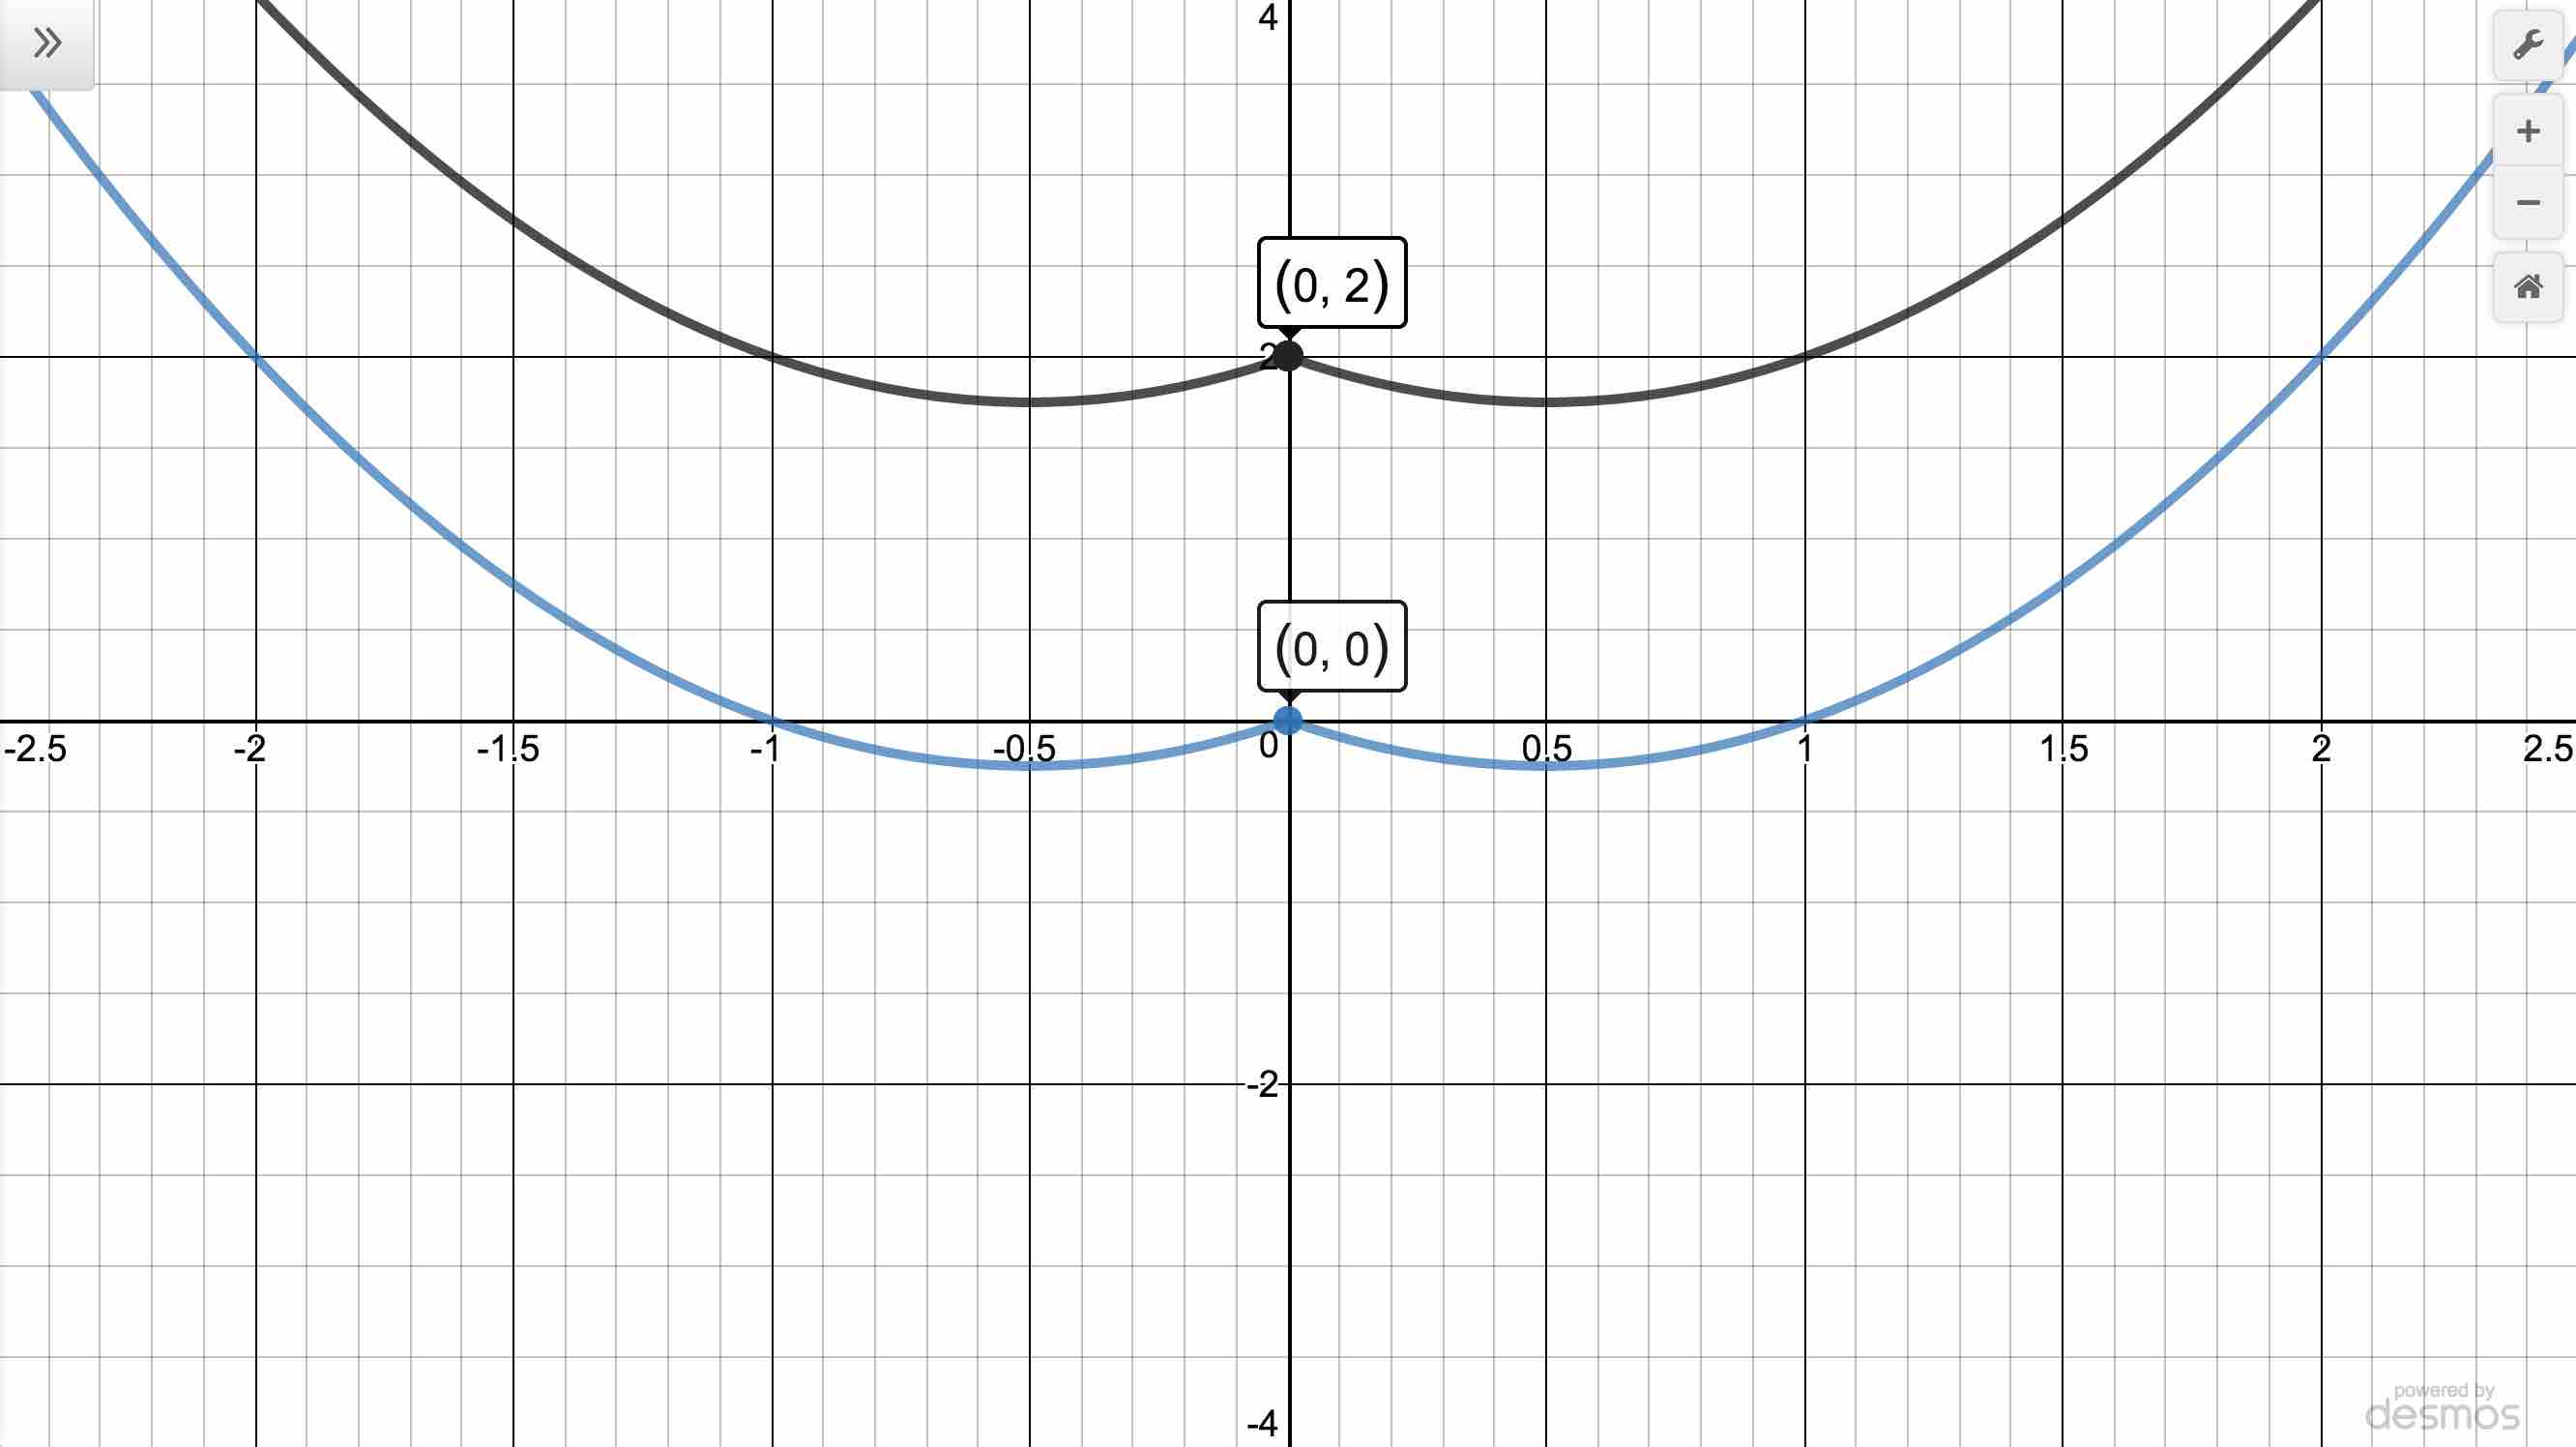
\includegraphics[width=3in]{./TransformationsGraphics/TransformationsEx04a.jpg} & 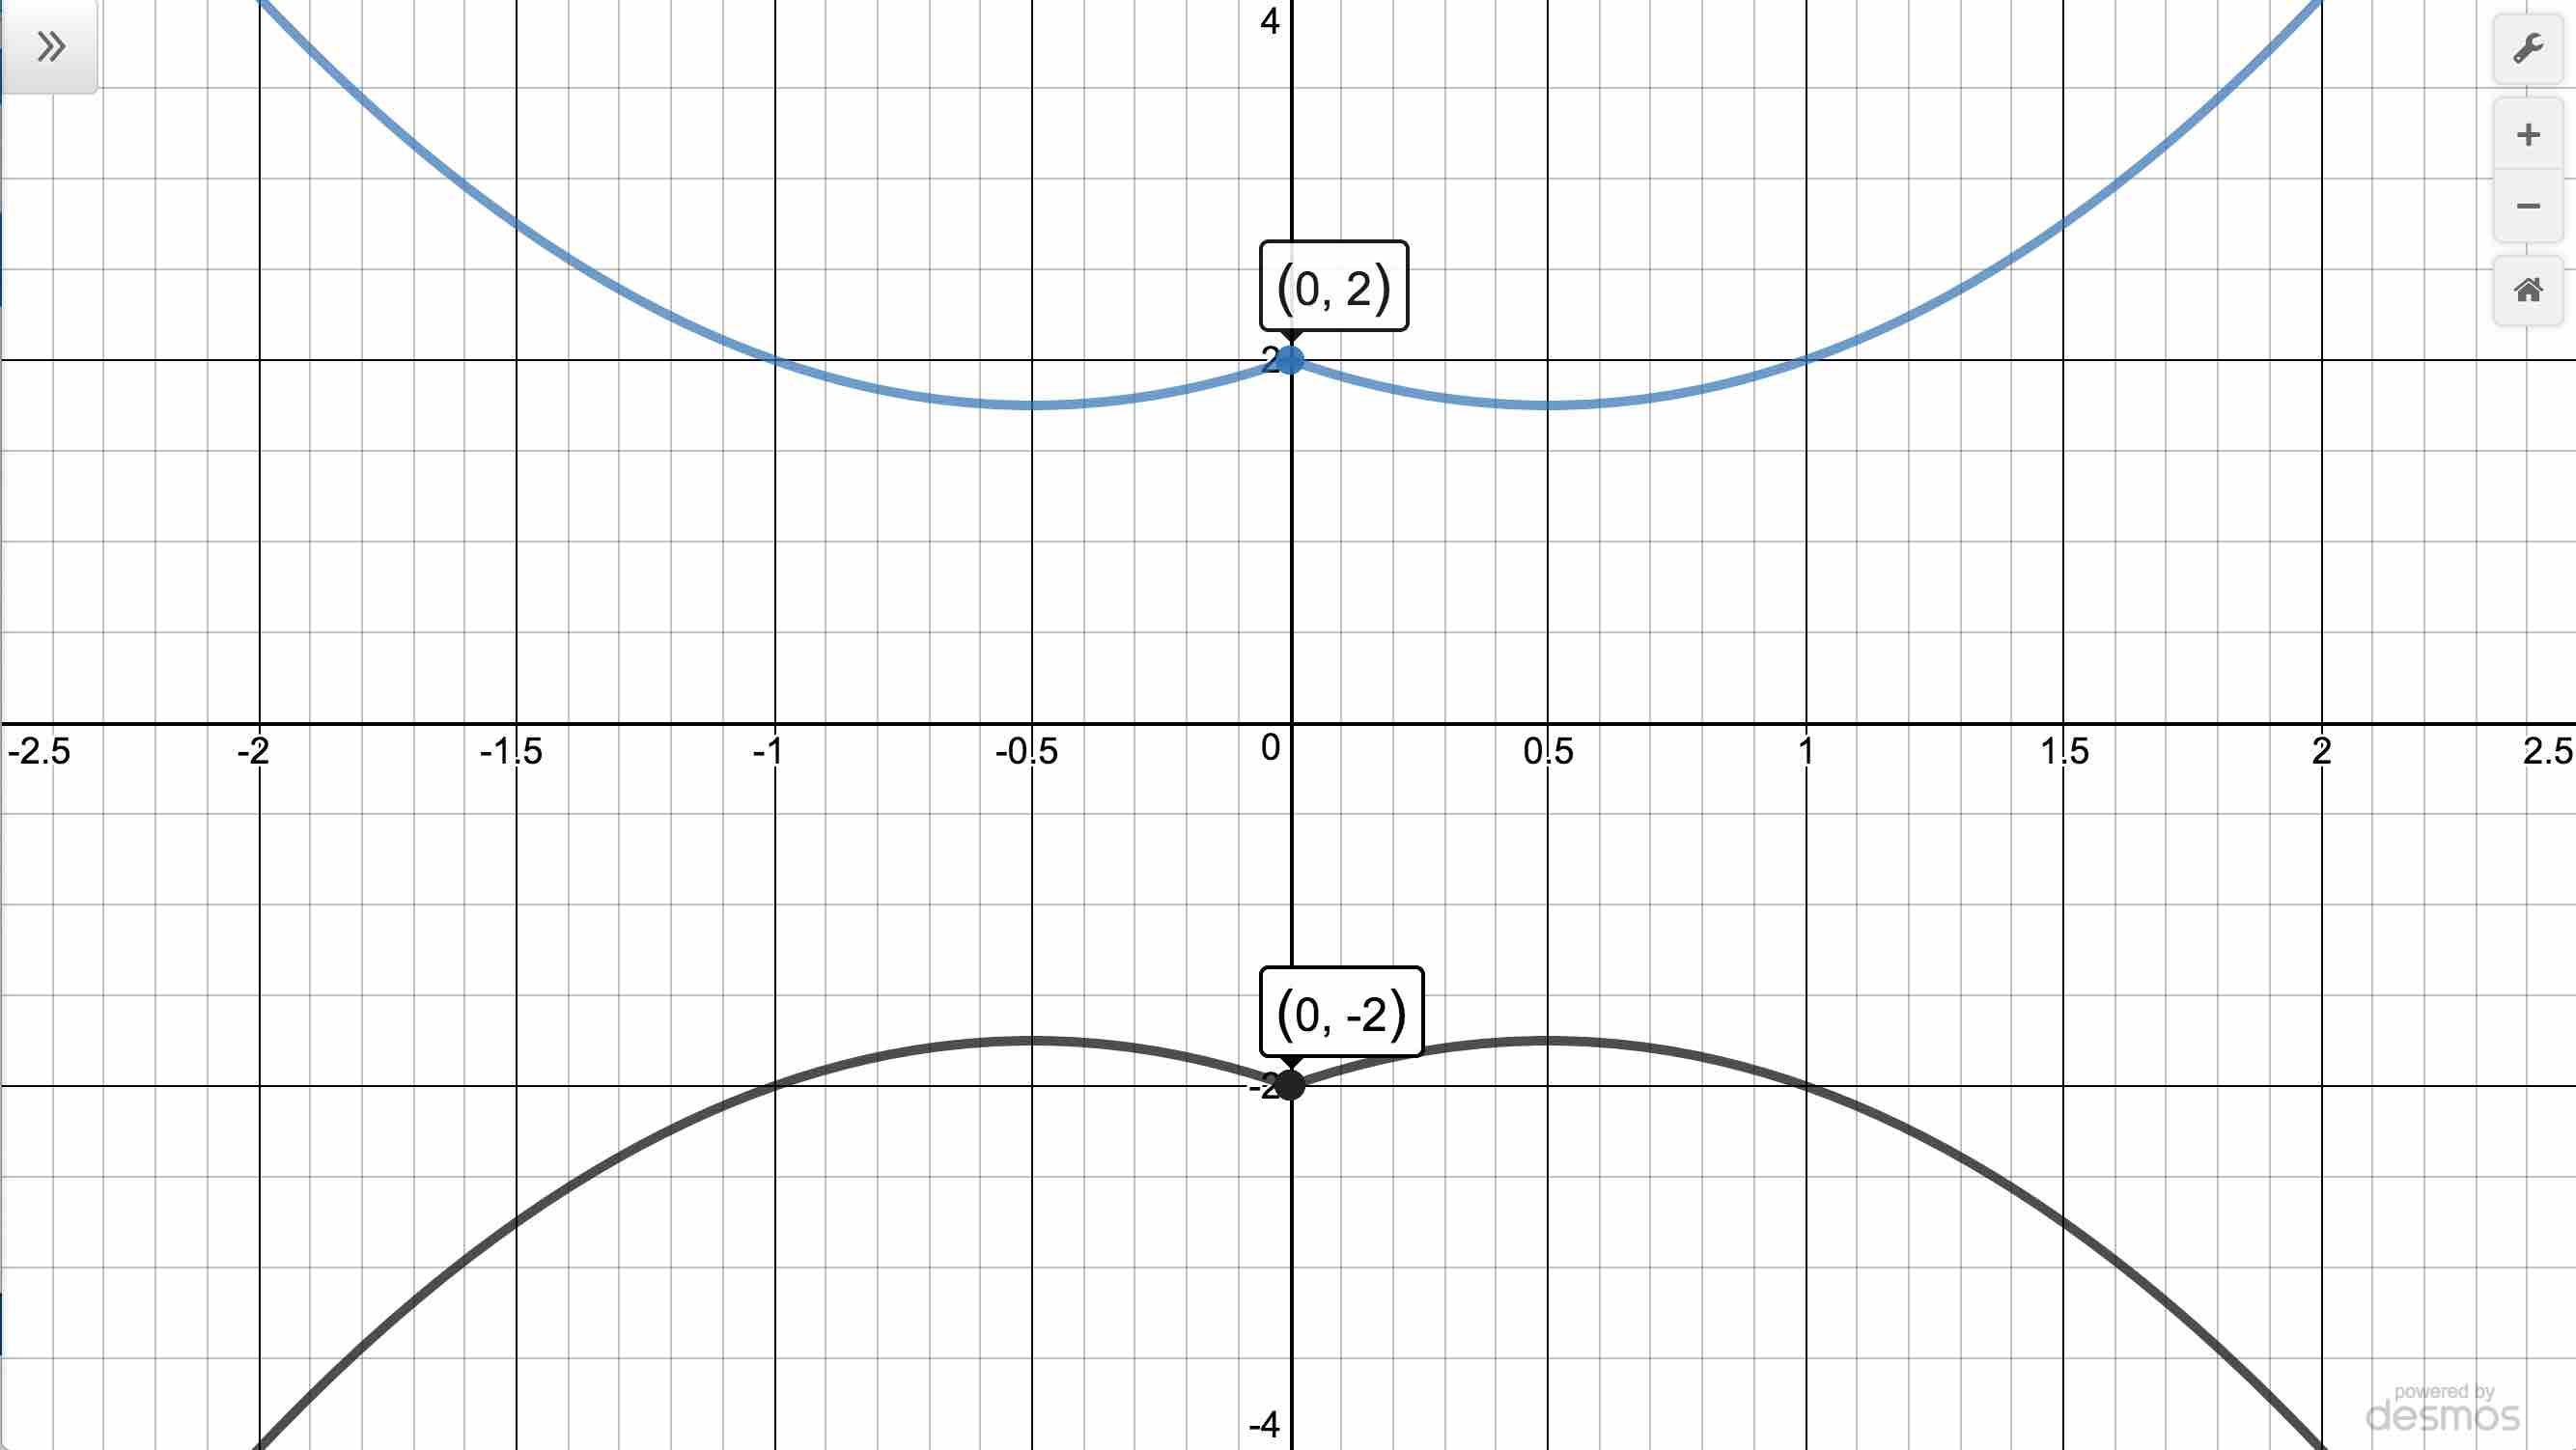
\includegraphics[width=3in]{./TransformationsGraphics/TransformationsEx04b.jpg} \\

$y=f(x)$ (lighter color) and $y=g_{1}(x) = f(x)+2$ &  $y = g_{1}(x)$ (lighter color) and $y = g_{2}(x) = -g_{1}(x)$ \\

\end{tabular}

\end{center} 

\item  Per Theorem \ref{hshifts}, $g_{3}(x) = g_{2}(x-1) = -(x-1)^2+|x-1|-2$.

\item  Per Theorem \ref{hscalings}, $g_{4}(x) = g_{3}(2x) = -(2x-1)^2+|2x-1| - 2$.

\begin{center}

\begin{tabular}{cc}

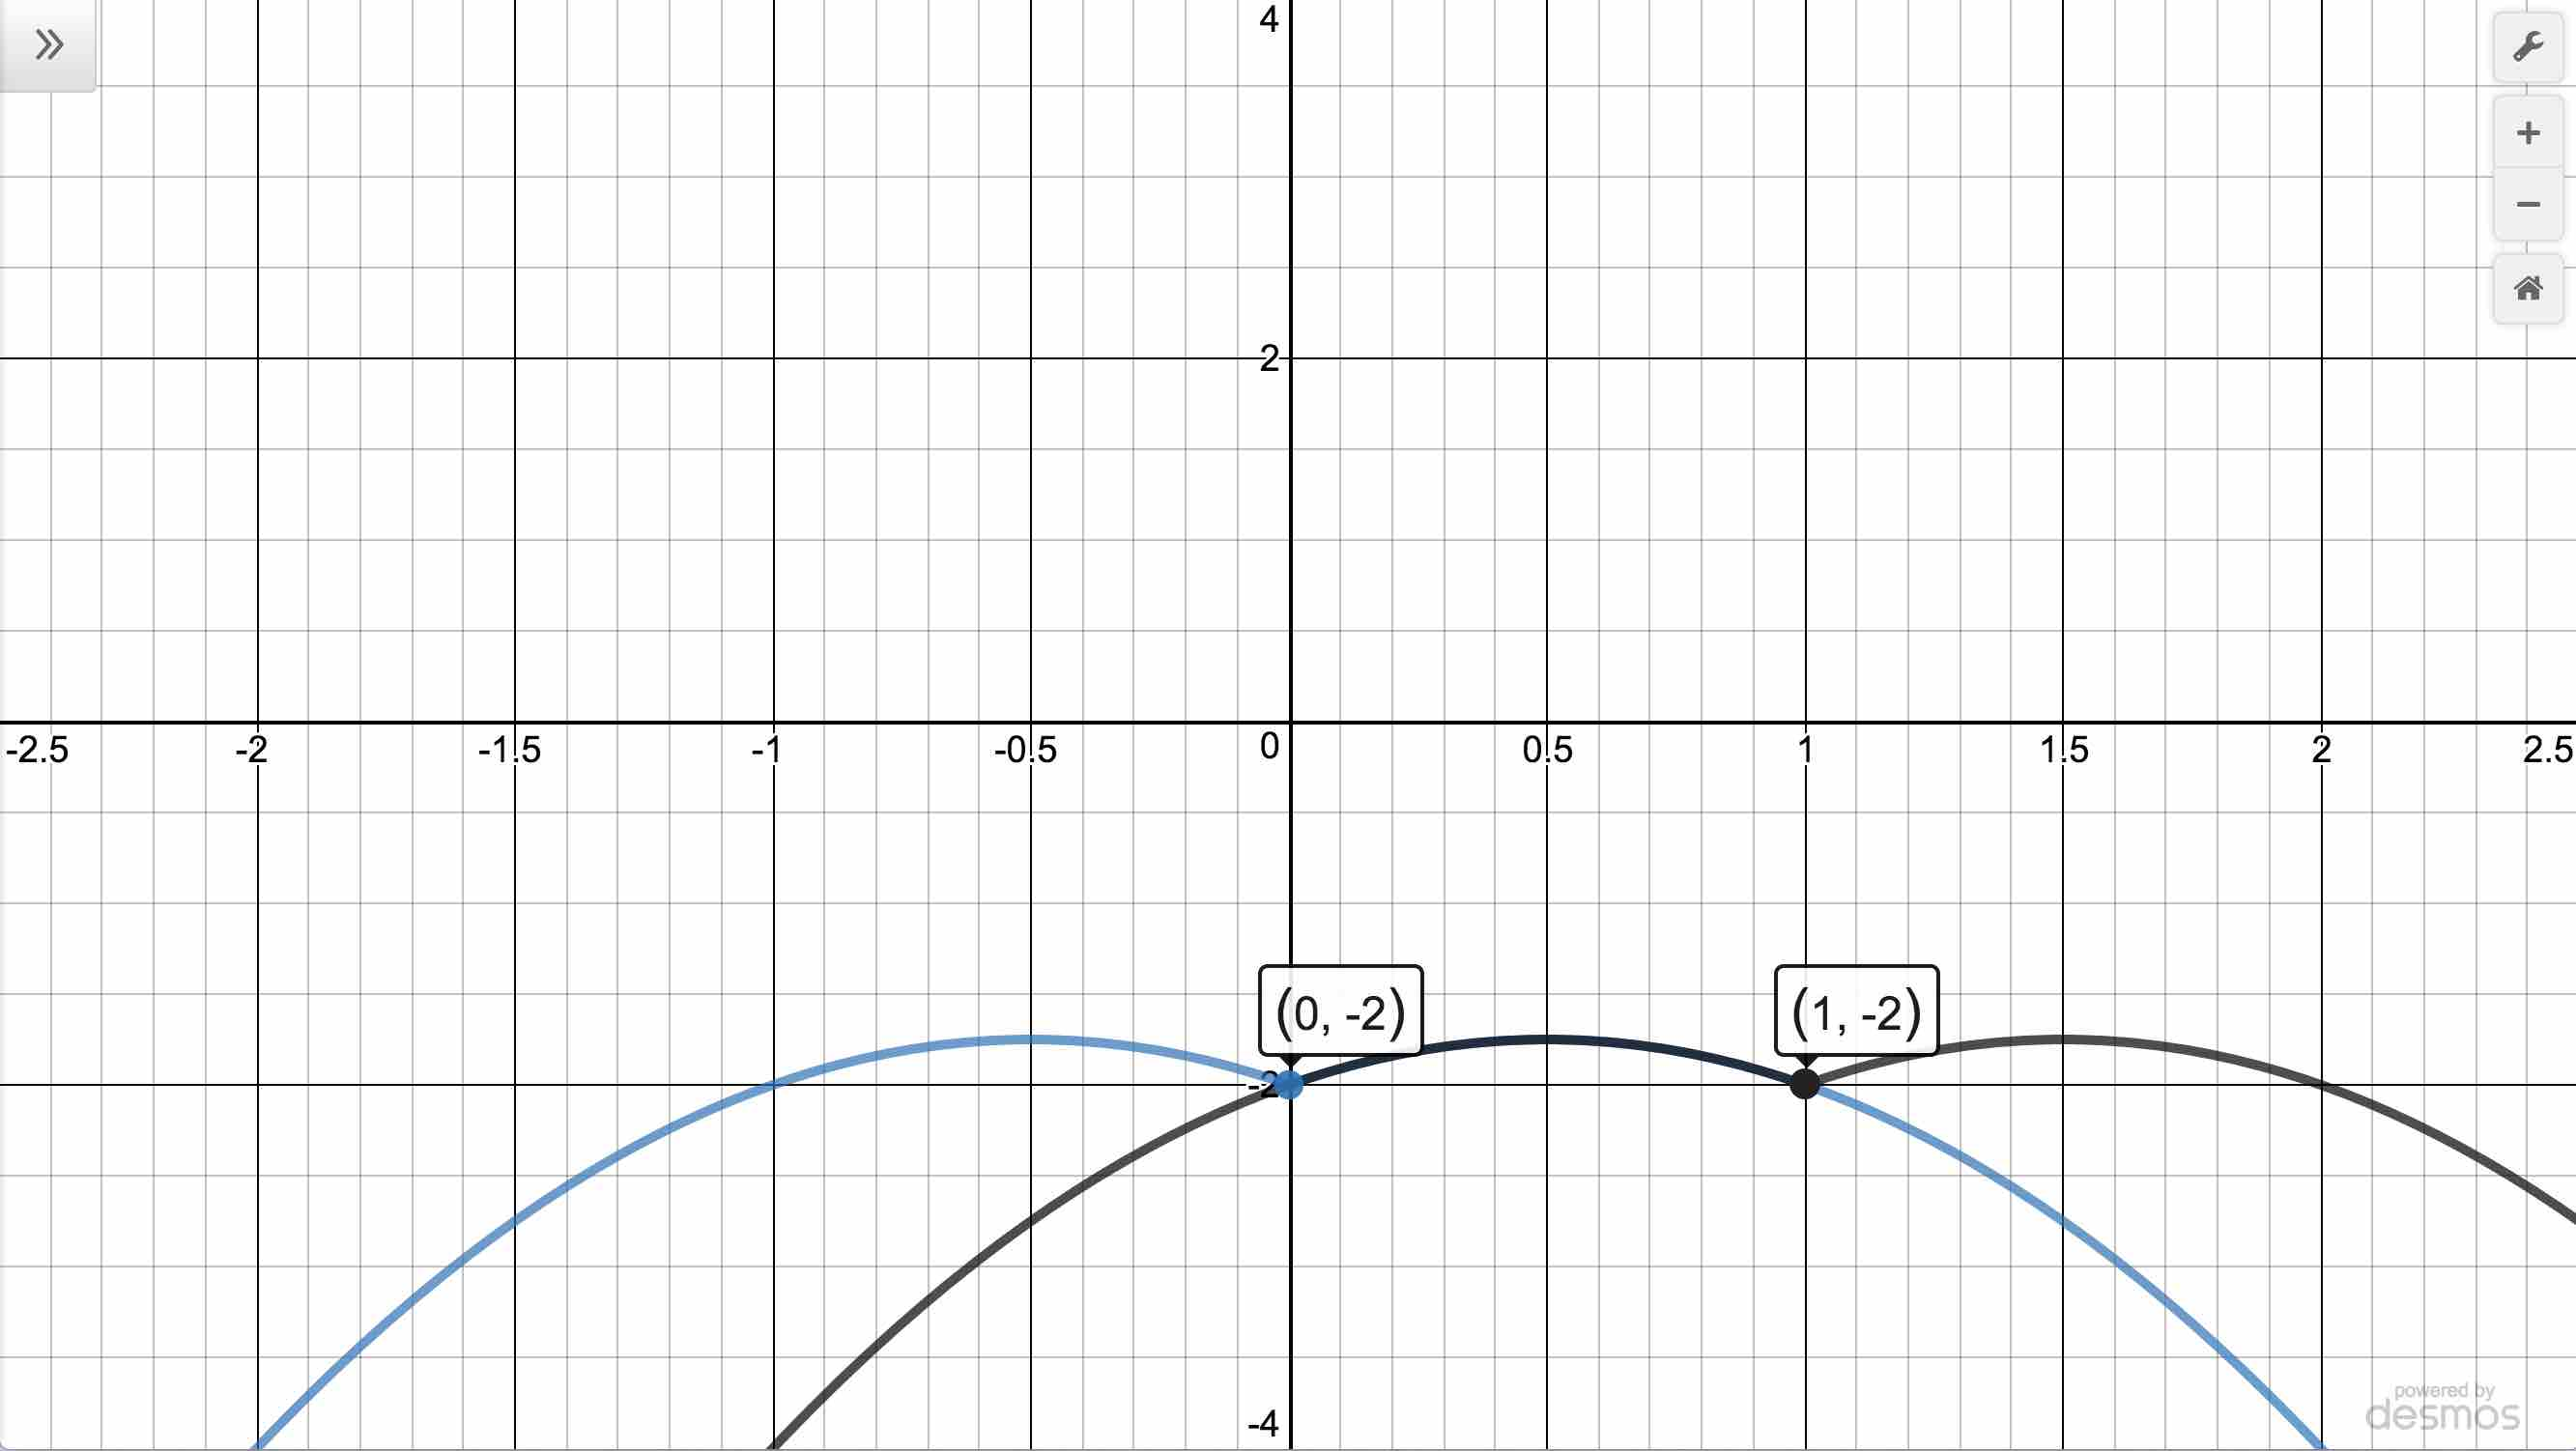
\includegraphics[width=3in]{./TransformationsGraphics/TransformationsEx04c.jpg} & 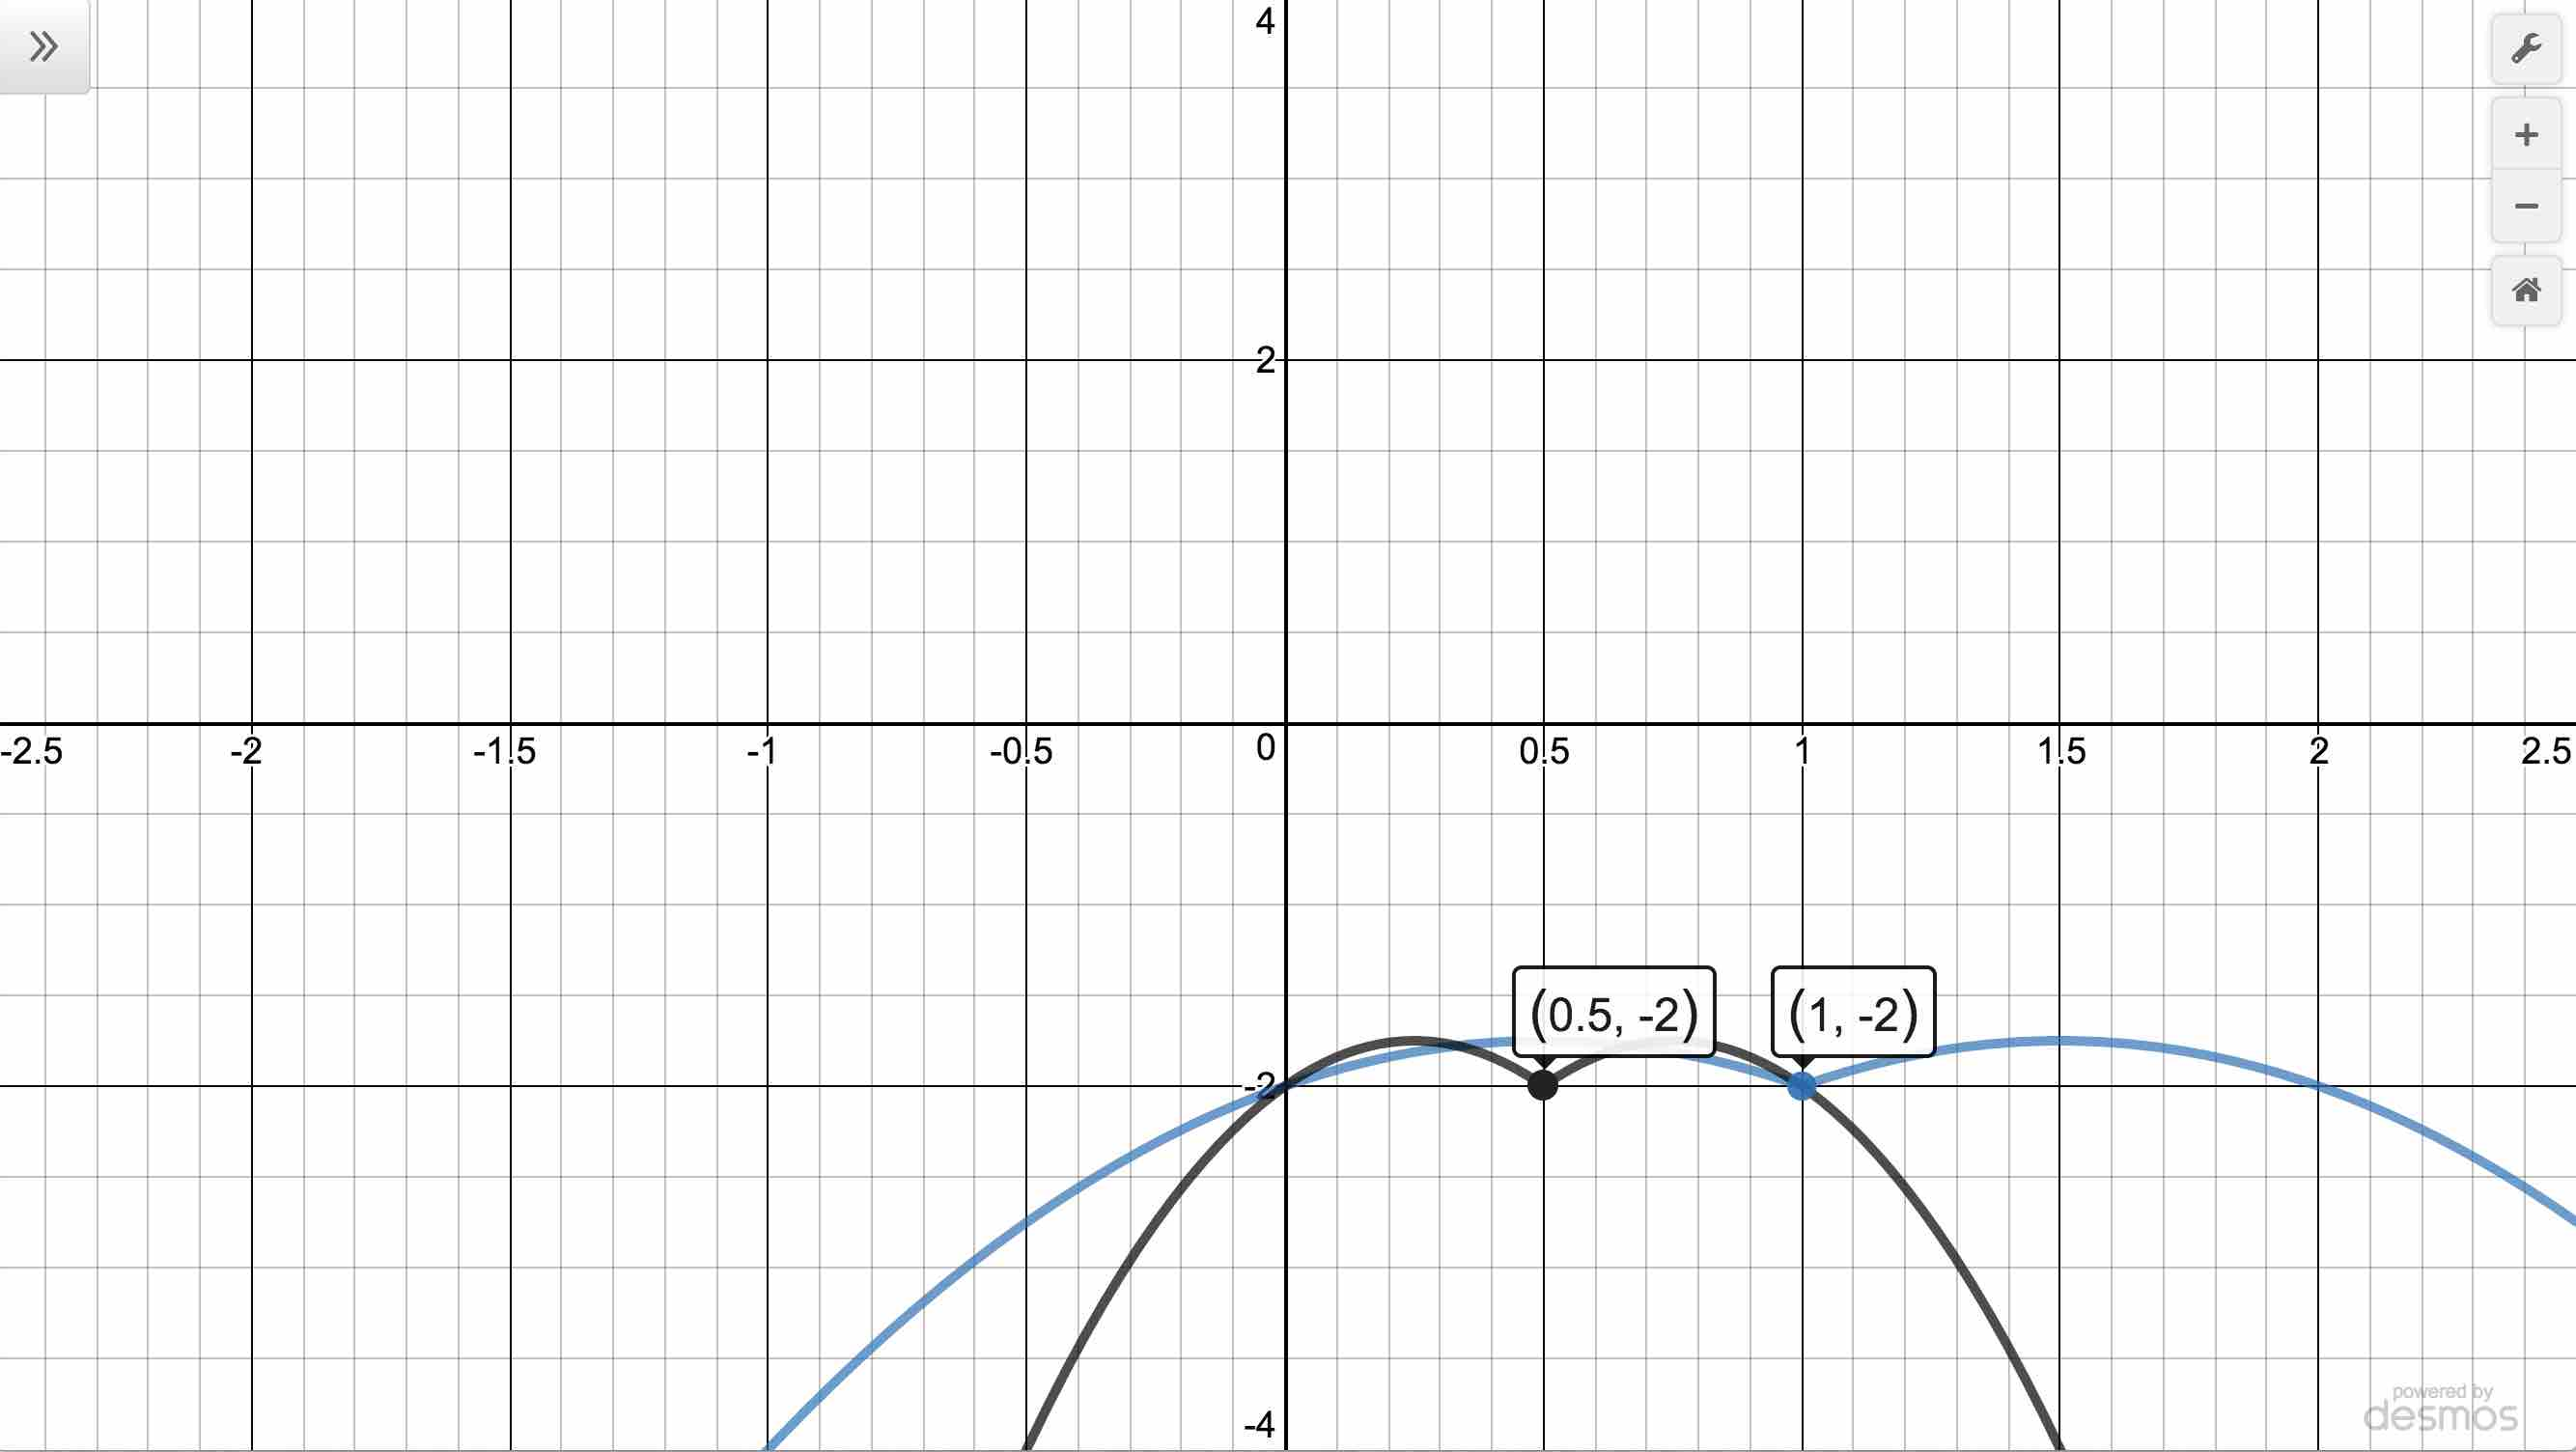
\includegraphics[width=3in]{./TransformationsGraphics/TransformationsEx04d.jpg} \\

$y=g_{2}(x)$ (lighter color) and $y=g_{3}(x) = g_{2}(x-1)$ &  $y = g_{3}(x)$ (lighter color) and $y = g_{4}(x) = g_{3}(2x)$ \\

\end{tabular}

\end{center} 

\item  Per Theorem \ref{vshifts}, $g_{5}(x) = g_{4}(x)+3 =  -(2x-1)^2+|2x-1| - 2 + 3 =  -(2x-1)^2+|2x-1| +1$.

\item  Per Theorem \ref{reflections}, $g_{6}(x) = g_{5}(-x)$:

\[ \begin{array}{rcl}

g_{6}(x) & = & g_{5}(-x) \\
 &  = &  -(2(-x)-1)^2+|2(-x)-1|+1 \\
  &  = & -(-2x-1)^2+|-2x-1|+1 \\
  &  = &  -[(-1)(2x+1)]^2+|[(-1)(2x+1)|+1 \\
  &  = &   -(-1)^2(2x+1)^2+|-1||2x+1| + 1 \\
  & =  & -(2x+1)^2+|2x+1|+1 \\
  
  \end{array} \]

\begin{center}

\begin{tabular}{cc}

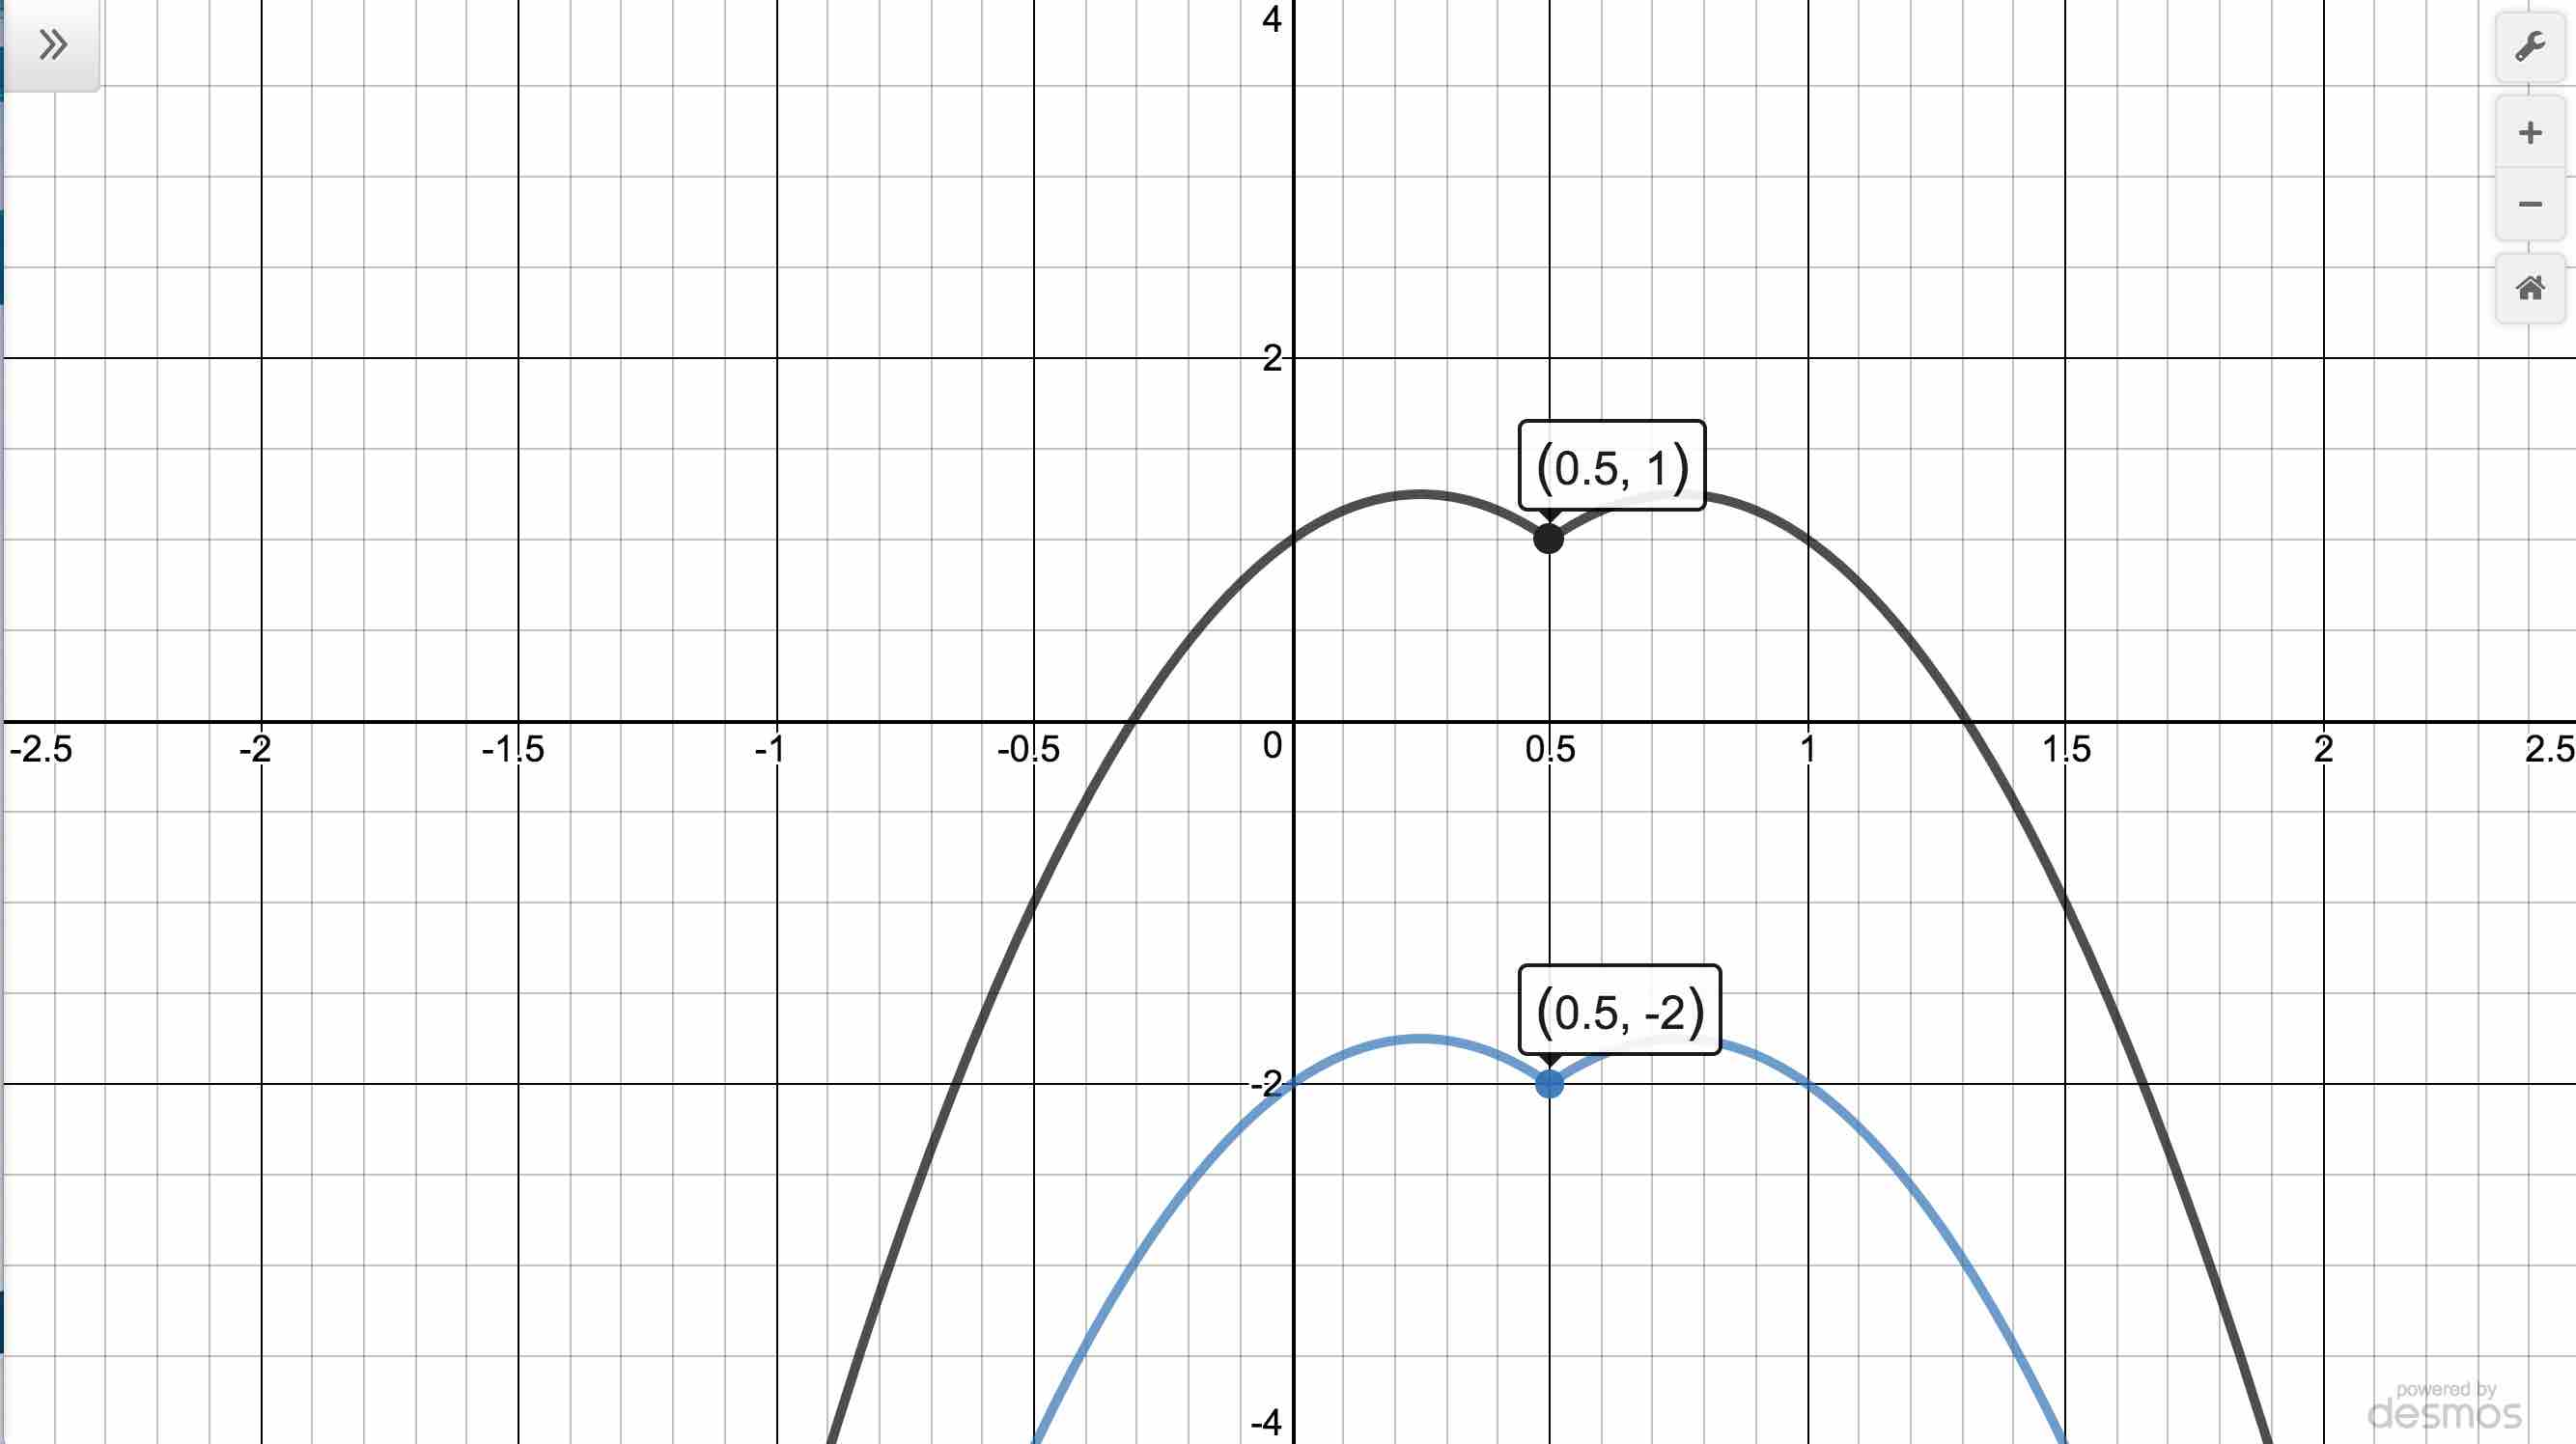
\includegraphics[width=3in]{./TransformationsGraphics/TransformationsEx04e.jpg} & 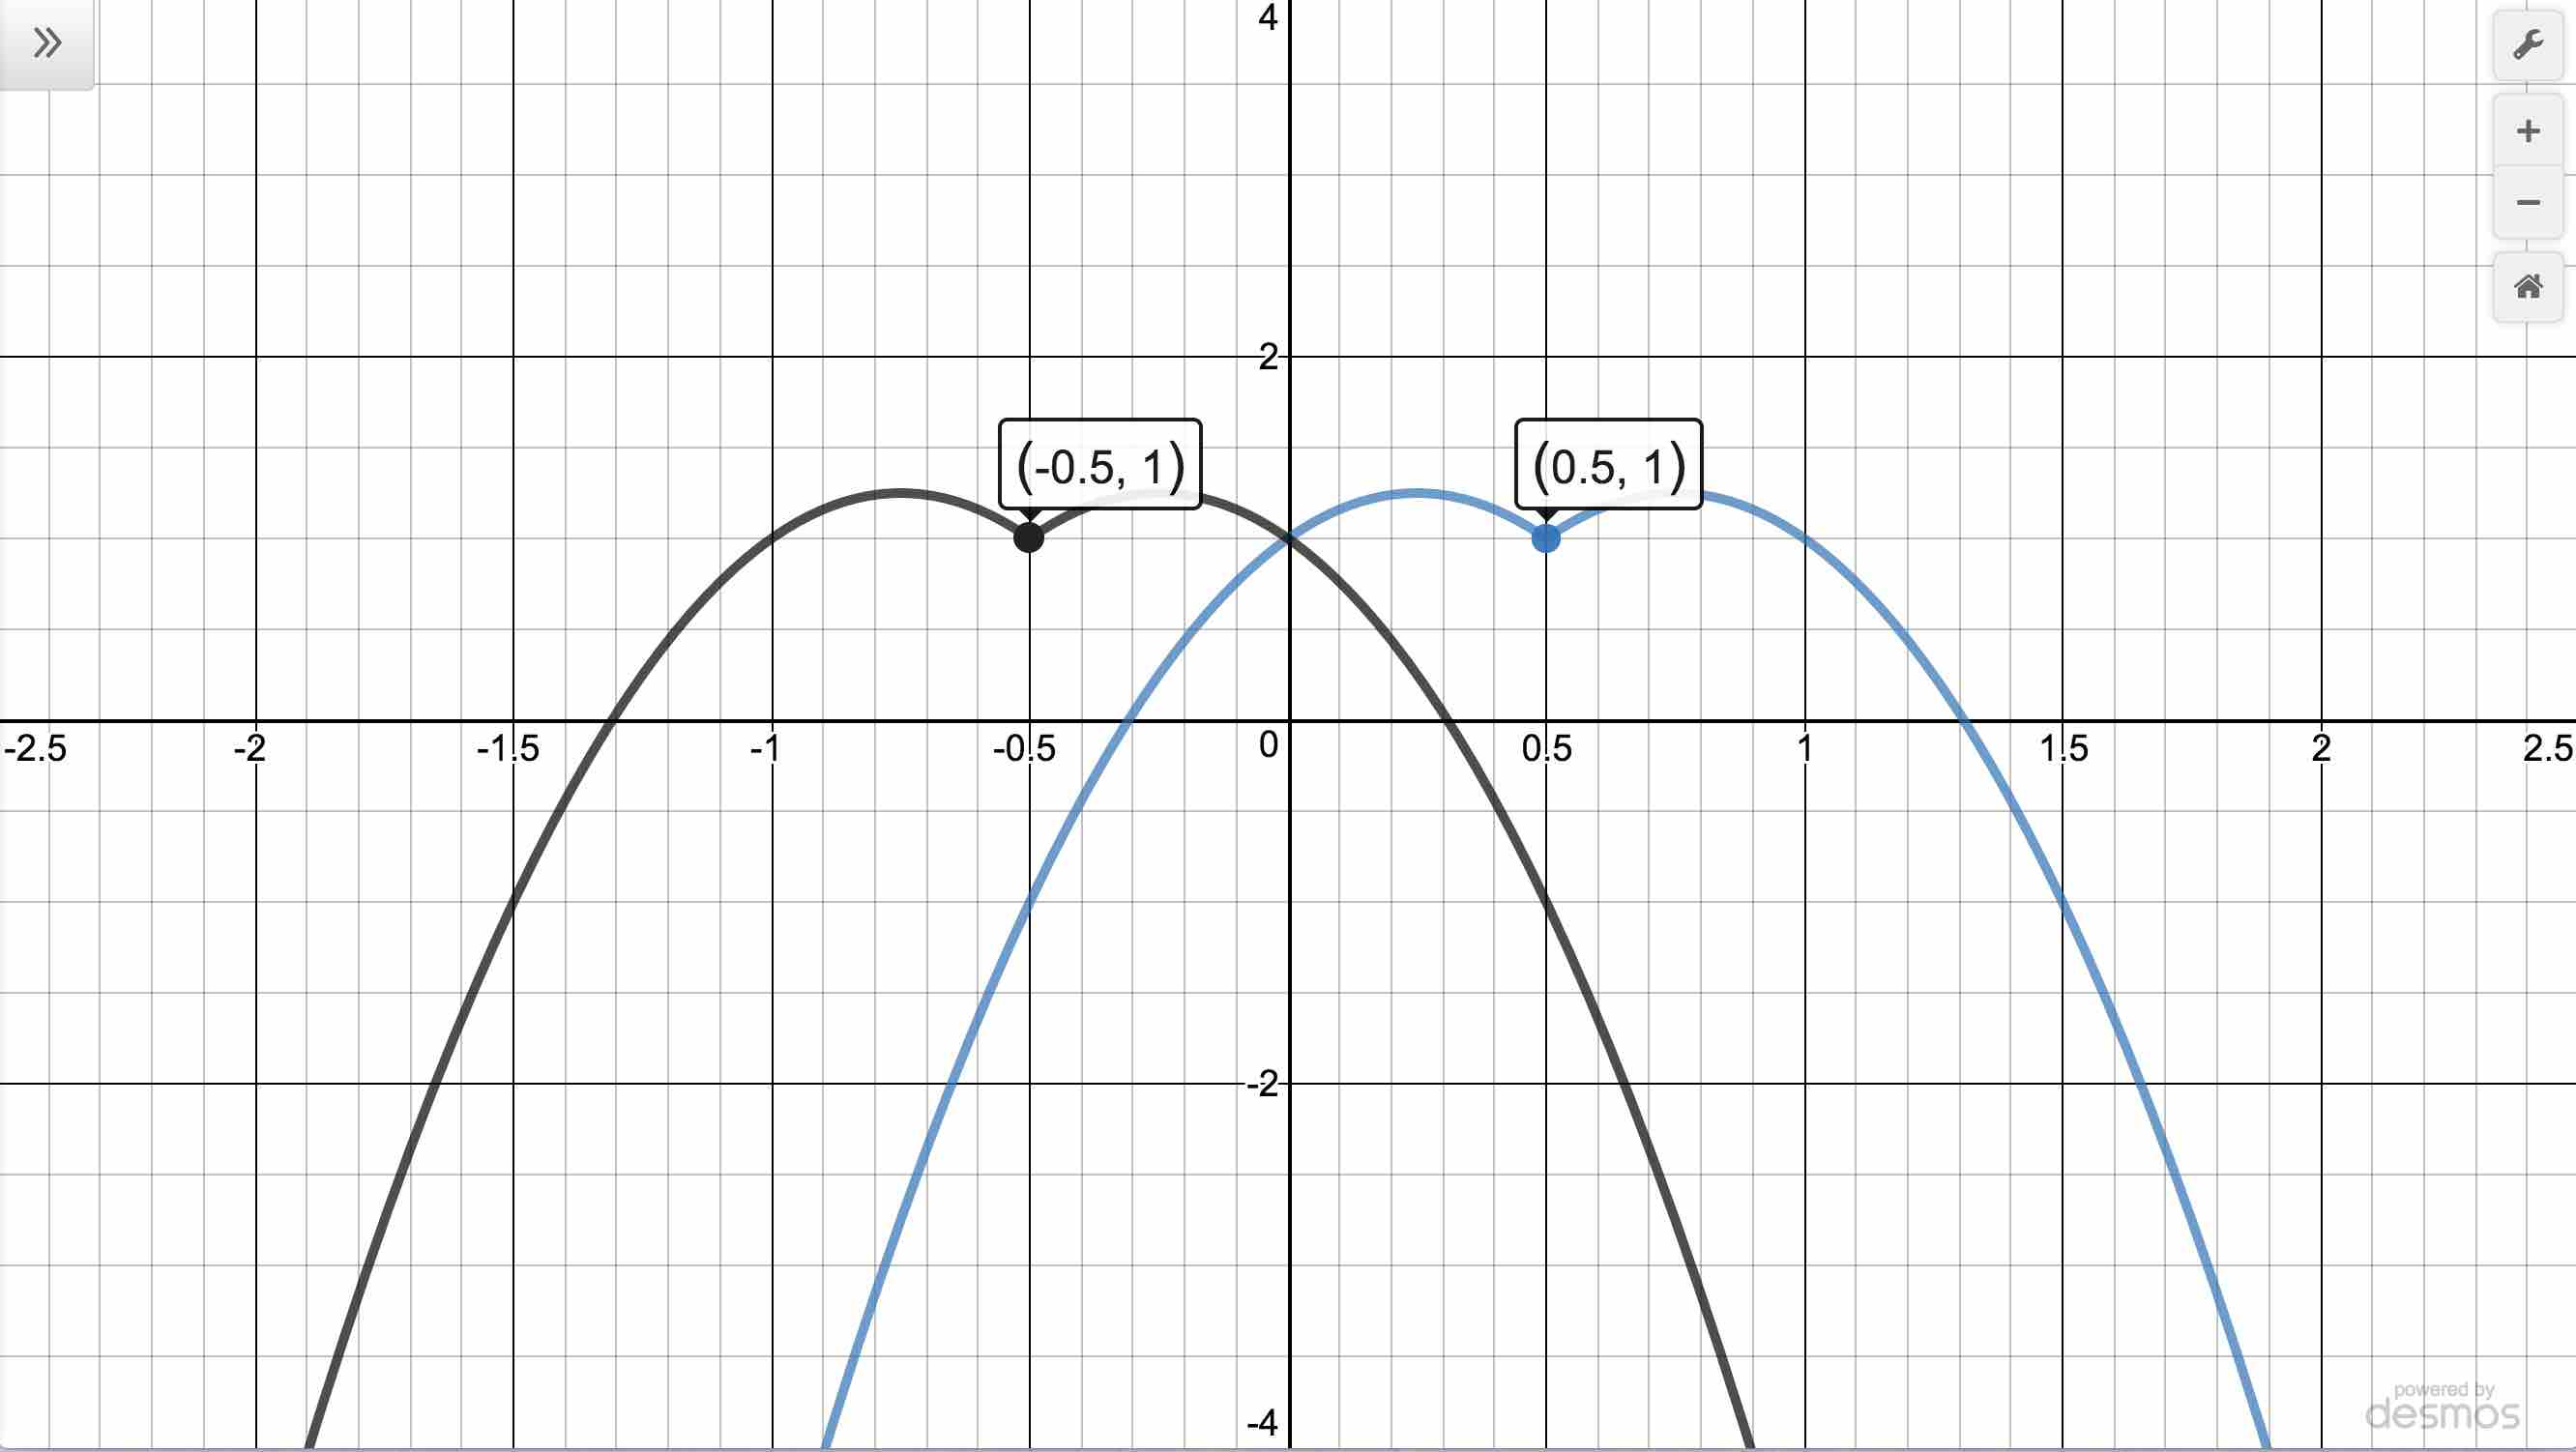
\includegraphics[width=3in]{./TransformationsGraphics/TransformationsEx04f.jpg} \\

$y=g_{4}(x)$ (lighter color) and $y=g_{5}(x) = g_{4}(x)+3$ &  $y = g_{5}(x)$ (lighter color) and $y = g_{6}(x) = g_{5}(-x)$ \\

\end{tabular}

\end{center} 

\end{enumerate}

Hence, $g(x) = g_{6}(x) = -(2x+1)^2+|2x+1| + 1$.  \qed
 
\end{ex}

It is instructive to show that the expression $g(x)$ in Example \ref{transsequenceex}  can be written as $g(x) = a f(bx-h)+k$.  

\smallskip

One way is to compare the graphs of $f$ and $g$ and work backwards.  A more methodical way is to repeat the work of Example \ref{transsequenceex}, but never substitute the formula for $f(x)$ as follows:


\begin{enumerate}

\item  Per Theorem \ref{vshifts}, $g_{1}(x) = f(x) + 2$.

\item  Per Theorem \ref{reflections}, $g_{2}(x) = -g_{1}(x) =  -[f(x) + 2] = -f(x)-2$.

\item  Per Theorem \ref{hshifts}, $g_{3}(x) = g_{2}(x-1) = -f(x-1)-2$.

\item  Per Theorem \ref{hscalings}, $g_{4}(x) = g_{3}(2x) =-f(2x-1)-2$.

\item  Per Theorem \ref{vshifts}, $g_{5}(x) = g_{4}(x)+3 = -f(2x-1)-2 + 3 = -f(2x-1)+1$.

\item  Per Theorem \ref{reflections}, $g_{6}(x) = g_{5}(-x) =  -f(2(-x)-1)+1 = -f(-2x-1)+1$.

\end{enumerate}

Hence $g(x) =  -f(-2x-1)+1$.  Note we can show $f$ is even,\footnote{Recall this means $f(-x) = f(x)$.} so $f(-2x-1) = f(-(2x+1)) = f(2x+1)$ and obtain $g(x) = -f(2x+1)+1$.  


At the beginning of this section, we discussed how all of the transformations we'd be discussing are the result of composing given functions with linear functions.  Not all transformations, not even all rigid transformations,\footnote{See Section \ref{PolarGraphs}.} fall into these categories.  

\smallskip

For example, consider the graphs of $y=f(x)$ and $y=g(x)$ below.

\[ \begin{array}{ccc}
\phantomsection
\label{relatedbyabsgraphs}
\begin{mfpic}[14]{-1}{6}{-6}{6}
\tlabel[cc](1,-5){\scriptsize $(0,-5)$}
\tlabel[cc](1,0.5){\scriptsize $(2,0)$}
\tlabel[cc](3,3){\scriptsize $(4,3)$}
\tlabel[cc](6,3){\scriptsize $(5,3)$}
\tlabel[cc](6,-0.5){\scriptsize $x$}
\tlabel[cc](0.5,6){\scriptsize $y$}
\tcaption{\scriptsize $y=f(x)$}
\axes
\xmarks{1,2,3,4,5}
\ymarks{-1,-2,-3,-4,-5,1,2,3,4,5}
\tlpointsep{4pt}
\axislabels {x}{{\scriptsize $1$} 1,  {\scriptsize $3$} 3, {\scriptsize $4$} 4, {\scriptsize $5$} 5}
\axislabels {y}{{\scriptsize $-1$} -1,{\scriptsize $-2$} -2, {\scriptsize $-3$} -3, {\scriptsize $-4$} -4,  {\scriptsize $1$} 1,{\scriptsize $2$} 2, {\scriptsize $3$} 3, {\scriptsize $4$} 4, {\scriptsize $5$} 5, {\scriptsize $-5$} -5}
\penwd{1.25pt}
\polyline{(0,-5), (2,0), (4,3), (5,3)}
\point[4pt]{(0,-5), (2,0), (4,3), (5,3)}
\end{mfpic}

&

\stackrel{\stackrel{}{\xrightarrow{\hspace{1in}}}}{\mbox{}} 

&


\begin{mfpic}[14]{-1}{6}{-6}{6}
\tlabel[cc](1,5){\scriptsize $(0,5)$}
\tlabel[cc](2,-0.5){\scriptsize $(2,0)$}
\tlabel[cc](3,3){\scriptsize $(4,3)$}
\tlabel[cc](6,3){\scriptsize $(5,3)$}
\tlabel[cc](6,-0.5){\scriptsize $x$}
\tlabel[cc](0.5,6){\scriptsize $y$}
\tcaption{\scriptsize $y=g(x)$}
\axes
\xmarks{1,2,3,4,5}
\ymarks{-1,-2,-3,-4,-5,1,2,3,4,5}
\tlpointsep{4pt}
\axislabels {x}{{\scriptsize $1$} 1,  {\scriptsize $3$} 3, {\scriptsize $4$} 4, {\scriptsize $5$} 5}
\axislabels {y}{{\scriptsize $-1$} -1,{\scriptsize $-2$} -2, {\scriptsize $1$} 1, {\scriptsize $-3$} -3, {\scriptsize $-4$} -4,  {\scriptsize $-5$} -5,{\scriptsize $2$} 2, {\scriptsize $3$} 3, {\scriptsize $4$} 4}
\penwd{1.25pt}
\polyline{(0,5), (2,0), (4,3), (5,3)}
\point[4pt]{(0,5), (2,0), (4,3), (5,3)}
\end{mfpic}

\end{array}\]




In Exercise \ref{relatedbyabsexercise}, we explore a non-linear transformation and revisit the pair of functions $f$ and $g$ then.



\newpage

\subsection{Exercises}

\label{ExercisesforTransformations}

Suppose $(2,-3)$ is on the graph of $y = f(x)$.  In Exercises \ref{transformpointfirst} - \ref{transformpointlast}, use Theorem \ref{transformationsthm} to find a point on the graph of the given transformed function.  

\begin{multicols}{3}
\begin{enumerate}

\item $y = f(x)+3$ \label{transformpointfirst}
\item $y = f(x+3)$
\item $y = f(x)-1$

\setcounter{HW}{\value{enumi}}
\end{enumerate}
\end{multicols}

\begin{multicols}{3}
\begin{enumerate}
\setcounter{enumi}{\value{HW}}

\item $y = f(x-1)$
\item $y = 3f(x)$
\item $y = f(3x)$

\setcounter{HW}{\value{enumi}}
\end{enumerate}
\end{multicols}

\begin{multicols}{3}
\begin{enumerate}
\setcounter{enumi}{\value{HW}}

\item $y = -f(x)$
\item $y = f(-x)$
\item $y = f(x-3)+1$

\setcounter{HW}{\value{enumi}}
\end{enumerate}
\end{multicols}

\begin{multicols}{3}
\begin{enumerate}
\setcounter{enumi}{\value{HW}}

\item $y = 2f(x+1)$
\item $y = 10 - f(x)$
\item $y = 3f(2x) - 1$

\setcounter{HW}{\value{enumi}}
\end{enumerate}
\end{multicols}

\begin{multicols}{3}
\begin{enumerate}
\setcounter{enumi}{\value{HW}}

\item $y = \frac{1}{2} f(4-x)$
\item $y = 5f(2x+1) + 3$
\item $y = 2f(1-x) -1$

\setcounter{HW}{\value{enumi}}
\end{enumerate}
\end{multicols}

\begin{multicols}{3}
\begin{enumerate}
\setcounter{enumi}{\value{HW}}

\item $y =f\left(\dfrac{7-2x}{4}\right)$
\item $y = \dfrac{f(3x) - 1}{2}$
\item $y = \dfrac{4-f(3x-1)}{7}$ \label{transformpointlast}

\setcounter{HW}{\value{enumi}}
\end{enumerate}
\end{multicols}



The complete graph of $y = f(x)$ is given below.  In Exercises \ref{transformgraphfirst} - \ref{transformgraphlast}, use it and Theorem \ref{transformationsthm} to graph the given transformed function.

\vspace{-.1in}
\begin{center}

\begin{mfpic}[15]{-5}{5}{-1}{5}
\axes
\tlabel[cc](5,-0.25){\scriptsize $x$}
\tlabel[cc](0.25,5){\scriptsize $y$}
\tlabel[cc](-2.5,1.25){\scriptsize $(-2,2)$}
\tlabel[cc](0.75,-0.5){\scriptsize $(0,0)$}
\tlabel[cc](2.25,1.25){\scriptsize $(2,2)$}
\tcaption{The graph of $y = f(x)$ for Ex. \ref{transformgraphfirst} - \ref{transformgraphlast}}
\xmarks{-4,-3,-2,-1,2,3,4}
\ymarks{1,2,3,4}
\tlpointsep{5pt}
\scriptsize
\axislabels {x}{{$-4 \hspace{7pt}$} -4,{$-3 \hspace{7pt}$} -3, {$-2 \hspace{7pt}$} -2, {$-1 \hspace{7pt}$} -1, {$2$} 2,{$3$} 3,{$4$} 4}
\axislabels {y}{{$1$} 1, {$2$} 2, {$3$} 3, {$4$} 4}
\normalsize
\penwd{1.25pt}
\arrow \reverse \arrow \polyline{(-4,4), (0,0), (4,4)}
\point[4pt]{(-2,2), (0,0), (2,2)}
\end{mfpic} 

\end{center}

\begin{multicols}{3}
\begin{enumerate}
\setcounter{enumi}{\value{HW}}

\item $y = f(x) + 1$ \label{transformgraphfirst}
\item $y = f(x) - 2$
\item $y = f(x+1)$

\setcounter{HW}{\value{enumi}}
\end{enumerate}
\end{multicols}

\begin{multicols}{3}
\begin{enumerate}
\setcounter{enumi}{\value{HW}}

\item $y = f(x - 2)$
\item $y = 2f(x)$
\item $y = f(2x)$

\setcounter{HW}{\value{enumi}}
\end{enumerate}
\end{multicols}

\begin{multicols}{3}
\begin{enumerate}
\setcounter{enumi}{\value{HW}}

\item $y = 2 - f(x)$
\item $y = f(2-x)$
\item $y = 2-f(2-x)$ \label{transformgraphlast}

\setcounter{HW}{\value{enumi}}
\end{enumerate}
\end{multicols}


\begin{enumerate}
\setcounter{enumi}{\value{HW}}

\item \label{somegraphsthesame} Some of the answers to Exercises \ref{transformgraphfirst} - \ref{transformgraphlast} above should be the same.  Which ones match up?  What properties of the graph of $y=f(x)$ contribute to the duplication?

\item  The function $f$ used in  Exercises \ref{transformgraphfirst} - \ref{transformgraphlast} should look familiar.  What is $f(x)$?  How does this this explain some of the duplication in the answers to Exercises \ref{transformgraphfirst} - \ref{transformgraphlast} mentioned in Exercise \ref{somegraphsthesame}?

\setcounter{HW}{\value{enumi}}
\end{enumerate}

\newpage

The complete graph of $y =g(t)$ is given below.  In Exercises \ref{transsecondgraphfirst} - \ref{transsecondgraphlast}, use it and Theorem \ref{transformationsthm} to graph the given transformed function.

\vspace{-.1in}
\begin{center}

\begin{mfpic}[15]{-5}{5}{-5}{5}
\axes
\tlabel[cc](5,-0.25){\scriptsize $t$}
\tlabel[cc](0.25,5){\scriptsize $y$}
\tlabel[cc](-2.25,-1.25){\scriptsize $(-2,0)$}
\tlabel[cc](1,4){\scriptsize $(0,4)$}
\tlabel[cc](2,-1.25){\scriptsize $(2,0)$}
\tlabel[cc](4,-2.5){\scriptsize $(4,-2)$}
\tcaption{The graph of $y = g(t)$ for Ex. \ref{transsecondgraphfirst} - \ref{transsecondgraphlast}}
\xmarks{-4,-3,-2,-1,1,2,3,4}
\ymarks{-4,-3,-2,-1,1,2,3,4}
\tlpointsep{5pt}
\scriptsize
\axislabels {x}{{$-4 \hspace{7pt}$} -4,{$-3 \hspace{7pt}$} -3, {$-1 \hspace{7pt}$} -1,{$1$} 1,{$3$} 3,{$4$} 4}
\axislabels {y}{{$-4$} -4,{$-3$} -3,{$-2$} -2, {$-1$} -1, {$1$} 1, {$2$} 2, {$3$} 3, {$4$} 4}
\normalsize
\penwd{1.25pt}
\polyline{(-2,0), (0,4), (2,0), (4,-2)}
\point[4pt]{(-2,0), (0,4), (2,0), (4,-2)}
\end{mfpic} 

\end{center}

\begin{multicols}{3}
\begin{enumerate}
\setcounter{enumi}{\value{HW}}

\item  $y = g(t) - 1$ \label{transsecondgraphfirst}
\item  $y = g(t + 1)$
\item  $y = \frac{1}{2} g(t)$

\setcounter{HW}{\value{enumi}}
\end{enumerate}
\end{multicols}

\begin{multicols}{3}
\begin{enumerate}
\setcounter{enumi}{\value{HW}}

\item  $y = g(2t)$
\item  $y = - g(t)$
\item  $y = g(-t)$

\setcounter{HW}{\value{enumi}}
\end{enumerate}
\end{multicols}

\begin{multicols}{3}
\begin{enumerate}
\setcounter{enumi}{\value{HW}}

\item  $y = g(t+1) - 1$
\item  $y = 1 - g(t)$
\item  $y = \frac{1}{2}g(t+1)-1$ \label{transsecondgraphlast}

\setcounter{HW}{\value{enumi}}
\end{enumerate}
\end{multicols}

The complete graph of $y = f(x)$ is given below.  In Exercises \ref{transthirdgraphfirst} - \ref{transthirdgraphlast}, use it and Theorem \ref{transformationsthm} to graph the given transformed function.

\vspace{-.1in}
\begin{center}

\begin{mfpic}[20]{-4}{4}{-1.5}{4}
\axes
\tlabel[cc](-3,-1){\small $\left(-3, 0 \right)$}
\tlabel[cc](0.8,3.3){\small $\left(0, 3 \right)$}
\tlabel[cc](3,-1){\small $\left(3, 0 \right)$}
\tlabel[cc](4,-0.5){\scriptsize $x$}
\tlabel[cc](0.5,4){\scriptsize $y$}
\tcaption{The graph of $y = f(x)$ for Ex. \ref{transthirdgraphfirst} - \ref{transthirdgraphlast}}
\xmarks{-3,-2,-1,1,2,3}
\ymarks{-1,1,2,3}
\tlpointsep{5pt}
\scriptsize
\axislabels {x}{{$-3 \hspace{7pt}$} -3, {$-2 \hspace{7pt}$} -2, {$-1 \hspace{7pt}$} -1, {$1$} 1, {$2$} 2, {$3$} 3}
\axislabels {y}{{$-1$} -1, {$1$} 1, {$2$} 2}
\normalsize
\penwd{1.25pt}
\point[4pt]{(-3,0),(0,3)}
\parafcn{0,3.14159,0.1}{(3*cos(t), 3*sin(t))}
\pointfillfalse
\point[4pt]{(3,0)}
\end{mfpic}

\end{center}

\begin{multicols}{3}
\begin{enumerate}
\setcounter{enumi}{\value{HW}}

\item $g(x) = f(x) + 3$ \label{transthirdgraphfirst}
\item $h(x) = f(x) - \frac{1}{2}$
\item $j(x) = f\left(x - \frac{2}{3}\right)$

\setcounter{HW}{\value{enumi}}
\end{enumerate}
\end{multicols}

\begin{multicols}{3}
\begin{enumerate}
\setcounter{enumi}{\value{HW}}

\item $a(x) = f(x + 4)$
\item $b(x) = f(x + 1) - 1$ 
\item $c(x) = \frac{3}{5}f(x)$


\setcounter{HW}{\value{enumi}}
\end{enumerate}
\end{multicols}

\begin{multicols}{3}
\begin{enumerate}
\setcounter{enumi}{\value{HW}}


\item $d(x) = -2f(x)$
\item $k(x) = f\left(\frac{2}{3}x\right)$
\item $m(x) = -\frac{1}{4}f(3x)$

\setcounter{HW}{\value{enumi}}
\end{enumerate}
\end{multicols}

\begin{multicols}{3}
\begin{enumerate}
\setcounter{enumi}{\value{HW}}

\item $n(x) = 4f(x - 3) - 6$
\item $p(x) = 4 + f(1 - 2x)$
\item $q(x) = -\frac{1}{2}f\left(\frac{x + 4}{2}\right) - 3$ \label{transthirdgraphlast}

\setcounter{HW}{\value{enumi}}
\end{enumerate}
\end{multicols}

\newpage

The complete graph of $y = S(t)$ is given below. 

\vspace{-.1in}
\begin{center}

\begin{mfpic}[20]{-3}{3}{-4}{4}
\axes
\tlabel[cc](3,-0.25){\scriptsize $t$}
\tlabel[cc](0.25,4){\scriptsize $y$}
\tlabel[cc](-2,0.5){\scriptsize $(-2,0)$}
\tlabel[cc](-1,-3.5){\scriptsize $(-1,-3)$}
\tlabel[cc](0.5,0.25){\scriptsize $(0,0)$}
\tlabel[cc](1,3.5){\scriptsize $(1,3)$}
\tlabel[cc](2,-0.5){\scriptsize $(2,0)$}
\tcaption{The graph of $y=S(t)$}
\xmarks{-2,-1,1,2}
\ymarks{-3,-2,-1,1,2,3}
\tlpointsep{5pt}
\scriptsize
\axislabels {x}{{$-2 \hspace{7pt}$} -2,{$-1 \hspace{7pt}$} -1,{$1$} 1}
\axislabels {y}{{$-3$} -3,{$-2$} -2, {$-1$} -1, {$1$} 1, {$2$} 2, {$3$} 3}
\normalsize
\penwd{1.25pt}
\function{-2,2,0.1}{3*sin(1.570796327*x)}
\point[4pt]{(-2,0), (-1,-3), (0,0), (1,3), (2,0)}
\end{mfpic} 

\end{center}

The purpose of Exercises \ref{transformsinegraphfirst} - \ref{transformsinegraphlast} is to build up to the graph  of $y = \frac{1}{2}S(-t+1) + 1$  one step at a time.

\begin{multicols}{2}
\begin{enumerate}
\setcounter{enumi}{\value{HW}}

\item $y = S_{\text{\tiny $1$}}(t) = S(t + 1)$ \label{transformsinegraphfirst}
\item  $y = S_{\text{\tiny $2$}}(t) =  S_{\text{\tiny $1$}}(-t) = S(-t + 1)$

\setcounter{HW}{\value{enumi}}
\end{enumerate}
\end{multicols}

\begin{multicols}{2}
\begin{enumerate}
\setcounter{enumi}{\value{HW}}

\item  $y = S_{\text{\tiny $3$}}(t) = \frac{1}{2}  S_{\text{\tiny $2$}}(t) =  \frac{1}{2}S(-t+1)$
\item  $y = S_{\text{\tiny $4$}}(t) = S_{\text{\tiny $3$}}(t) + 1 = \frac{1}{2}S(-t+1) + 1$ \label{transformsinegraphlast}

\setcounter{HW}{\value{enumi}}
\end{enumerate}
\end{multicols}

Let $f(x) = \sqrt{x}$.  Find a formula for a function $g$ whose graph is obtained from $f$ from the given sequence of transformations. 

\begin{enumerate}
\setcounter{enumi}{\value{HW}}


\item  (1) shift right 2 units; (2) shift down 3 units

\item  (1) shift down 3 units; (2) shift right 2 units

\item  (1) reflect across the $x$-axis; (2) shift up 1 unit

\item  (1) shift up 1 unit; (2) reflect across the $x$-axis

\item  (1) shift left 1 unit; (2) reflect across the $y$-axis; (3) shift up 2 units

\item  (1) reflect across the $y$-axis;  (2) shift left 1 unit;  (3) shift up 2 units

\item  (1) shift left 3 units; (2) vertical stretch by a factor of 2; (3) shift down 4 units

\item  (1) shift left 3 units; (2) shift down 4 units; (3) vertical stretch by a factor of 2

\item  (1) shift right 3 units; (2) horizontal shrink by a factor of 2; (3) shift up 1 unit

\item  (1) horizontal shrink by a factor of 2; (2) shift right 3 units; (3) shift up 1 unit


\setcounter{HW}{\value{enumi}}
\end{enumerate}


\newpage

For Exercises \ref{findformulatransformationfirst} - \ref{findformulatransformationlast},  use the given of  $y = f(x)$ to write each function in terms of $f(x)$.
\begin{center}

\begin{mfpic}[15]{-5}{5}{-5}{5}
\axes
\tlabel[cc](5,-0.25){\scriptsize $x$}
\tlabel[cc](0.25,5){\scriptsize $y$}
\tlabel[cc](-2,-1.5){\scriptsize $\left(-\frac{1}{2},-\frac{3}{2} \right)$}
\tlabel[cc](-0.75,0.5){\scriptsize $(0,0)$}
\tlabel[cc](1.75,1.5){\scriptsize $\left(\frac{1}{2},\frac{3}{2} \right)$}
\tlabel[cc](3, 3.5){\scriptsize asymptote $y=3$}
\tlabel[cc](-2.75,-3.5){\scriptsize asymptote $y=-3$}
\tcaption{The graph of $y = f(x)$  for Ex. \ref{findformulatransformationfirst} - \ref{findformulatransformationlast}.}
\xmarks{-4,-3,-2,-1,1,2,3,4}
\ymarks{-4,-3,-2,-1,1,2,3,4}
\tlpointsep{5pt}
\scriptsize
%\axislabels {x}{{$-4 \hspace{7pt}$} -4,{$-3 \hspace{7pt}$} -3, {$-1 \hspace{7pt}$} -1,{$1$} 1,{$3$} 3,{$4$} 4}
%\axislabels {y}{{$-4$} -4,{$-3$} -3,{$-2$} -2, {$-1$} -1, {$1$} 1, {$2$} 2, {$3$} 3, {$4$} 4}
\normalsize
\dashed \polyline {(-5,3), (5,3)}
\dashed \polyline {(-5,-3), (5,-3)}
\penwd{1.25pt}
\arrow \reverse \arrow \parafcn{-2.8,2.8,0.1}{( 0.5*(tan( 0.5236*t))   ,   t   )}
\point[4pt]{(0,0), (0.5,1.5), (-0.5,-1.5)}
\end{mfpic} 

\end{center}

%\enlargethispage{1in}

\begin{multicols}{2}
\begin{enumerate}
\setcounter{enumi}{\value{HW}}

\item  \label{findformulatransformationfirst} $y = g(x)$ %$g(x)=f(x)+1$

\begin{mfpic}[15]{-5}{5}{-5}{5}
\axes
\tlabel[cc](5,-0.25){\scriptsize $x$}
\tlabel[cc](0.25,5){\scriptsize $y$}
\tlabel[cc](-2,-0.5){\scriptsize $\left(-\frac{1}{2},-\frac{1}{2} \right)$}
\tlabel[cc](-0.75,1.5){\scriptsize $(0,1)$}
\tlabel[cc](1.75,2.5){\scriptsize $\left(\frac{1}{2},\frac{5}{2} \right)$}
\tlabel[cc](3, 4.5){\scriptsize asymptote $y=4$}
\tlabel[cc](-2.75,-2.5){\scriptsize asymptote $y=-2$}
\xmarks{-4,-3,-2,-1,1,2,3,4}
\ymarks{-4,-3,-2,-1,1,2,3,4}
\tlpointsep{5pt}
\scriptsize
%\axislabels {x}{{$-4 \hspace{7pt}$} -4,{$-3 \hspace{7pt}$} -3, {$-1 \hspace{7pt}$} -1,{$1$} 1,{$3$} 3,{$4$} 4}
%\axislabels {y}{{$-4$} -4,{$-3$} -3,{$-2$} -2, {$-1$} -1, {$1$} 1, {$2$} 2, {$3$} 3, {$4$} 4}
\normalsize
\dashed \polyline {(-5,4), (5,4)}
\dashed \polyline {(-5,-2), (5,-2)}
\penwd{1.25pt}
\arrow \reverse \arrow \parafcn{-2.8,2.8,0.1}{( 0.5*(tan( 0.5236*t))   ,   t +1  )}
\point[4pt]{(0,1), (0.5,2.5), (-0.5,-0.5)}
\end{mfpic} 


\item  $y = h(x)$ %$h(x) = f(x-2)$

\begin{mfpic}[15]{-3}{7}{-5}{5}
\axes
\tlabel[cc](7,-0.25){\scriptsize $x$}
\tlabel[cc](0.25,5){\scriptsize $y$}
\gclear \tlabelrect(0,-1.5){\scriptsize $\left(\frac{3}{2},-\frac{3}{2} \right)$}
\tlabel[cc](1.25,0.5){\scriptsize $(2,0)$}
\tlabel[cc](3.75,1.5){\scriptsize $\left(\frac{5}{2},\frac{3}{2} \right)$}
\tlabel[cc](3, 3.5){\scriptsize asymptote $y=3$}
\gclear \tlabelrect(-0.75,-3.5){\scriptsize asymptote $y=-3$}
\xmarks{-2,-1,1,2,3,4,5,6}
\ymarks{-3, 2,3,4}
\tlpointsep{5pt}
\scriptsize
%\axislabels {x}{{$-4 \hspace{7pt}$} -4,{$-3 \hspace{7pt}$} -3, {$-1 \hspace{7pt}$} -1,{$1$} 1,{$3$} 3,{$4$} 4}
%\axislabels {y}{{$-4$} -4,{$-3$} -3,{$-2$} -2, {$-1$} -1, {$1$} 1, {$2$} 2, {$3$} 3, {$4$} 4}
\normalsize
\dashed \polyline {(-3,3), (7,3)}
\dashed \polyline {(-3,-3), (7,-3)}
\penwd{1.25pt}
\arrow \reverse \arrow \parafcn{-2.8,2.8,0.1}{( 2+(0.5*(tan( 0.5236*t)))    ,   t   )}
\point[4pt]{(2,0), (2.5,1.5), (1.5,-1.5)}
\end{mfpic} 


\setcounter{HW}{\value{enumi}}
\end{enumerate}
\end{multicols}



\begin{multicols}{2}
\begin{enumerate}
\setcounter{enumi}{\value{HW}}

\item   $y = p(x)$  % $p(x) = f\left( \frac{x}{2} \right) -1$

\begin{mfpic}[15]{-5}{5}{-5}{5}
\axes
\tlabel[cc](5,-0.25){\scriptsize $x$}
\tlabel[cc](0.25,5){\scriptsize $y$}
\tlabel[cc](-2,-2.5){\scriptsize $\left(-1,-\frac{5}{2} \right)$}
\tlabel[cc](-1,-1){\scriptsize $(0,-1)$}
\tlabel[cc](1.75,0.5){\scriptsize $\left(1,\frac{1}{2} \right)$}
\tlabel[cc](3, 2.5){\scriptsize asymptote $y=2$}
\tlabel[cc](-2.75,-4.5){\scriptsize asymptote $y=-4$}
\xmarks{-4 step 0.5 until 4}
\ymarks{-4,-3,-2,-1,1,2,3,4}
\tlpointsep{5pt}
\scriptsize
%\axislabels {x}{{$-4 \hspace{7pt}$} -4,{$-3 \hspace{7pt}$} -3, {$-1 \hspace{7pt}$} -1,{$1$} 1,{$3$} 3,{$4$} 4}
%\axislabels {y}{{$-4$} -4,{$-3$} -3,{$-2$} -2, {$-1$} -1, {$1$} 1, {$2$} 2, {$3$} 3, {$4$} 4}
\normalsize
\dashed \polyline {(-5,2), (5,2)}
\dashed \polyline {(-5,-4), (5,-4)}
\penwd{1.25pt}
\arrow \reverse \arrow \parafcn{-2.8,2.8,0.1}{( 0.5*(tan( 0.5236*t))   ,   t -1  )}
\point[4pt]{(0,-1), (0.5,0.5), (-0.5,-2.5)}
\end{mfpic} 


\item  $y = q(x)$  % $q(x) = -2f(x) = 2f(-x)$


\begin{mfpic}[15]{-5}{5}{-5}{5}
\axes
\tlabel[cc](5,-0.25){\scriptsize $x$}
\tlabel[cc](0.25,5){\scriptsize $y$}
\tlabel[cc](-2,1.5){\scriptsize $\left(-\frac{1}{2},3 \right)$}
\tlabel[cc](0.75,0.5){\scriptsize $(0,0)$}
\tlabel[cc](1.75,-1.5){\scriptsize $\left(\frac{1}{2} -3 \right)$}
\tlabel[cc](3, 3.5){\scriptsize asymptote $y=6$}
\tlabel[cc](-2.75,-3.5){\scriptsize asymptote $y=-6$}
\xmarks{-4,-3,-2,-1,1,2,3,4}
\ymarks{-4 step 0.5 until 4}
\tlpointsep{5pt}
\scriptsize
%\axislabels {x}{{$-4 \hspace{7pt}$} -4,{$-3 \hspace{7pt}$} -3, {$-1 \hspace{7pt}$} -1,{$1$} 1,{$3$} 3,{$4$} 4}
%\axislabels {y}{{$-4$} -4,{$-3$} -3,{$-2$} -2, {$-1$} -1, {$1$} 1, {$2$} 2, {$3$} 3, {$4$} 4}
\normalsize
\dashed \polyline {(-5,3), (5,3)}
\dashed \polyline {(-5,-3), (5,-3)}
\penwd{1.25pt}
\arrow \reverse \arrow \parafcn{-2.8,2.8,0.1}{( 0.5*(tan( 0.5236*t))   ,  -1*t   )}
\point[4pt]{(0,0), (0.5,-1.5), (-0.5,1.5)}
\end{mfpic} 



\setcounter{HW}{\value{enumi}}
\end{enumerate}
\end{multicols}

\newpage

\begin{multicols}{2}
\begin{enumerate}
\setcounter{enumi}{\value{HW}}

\item  $y = r(x)$ % $r(x) = 2f(x+1)-3$

\begin{mfpic}[15]{-6}{4}{-5}{5}
\axes
\tlabel[cc](4,-0.25){\scriptsize $x$}
\tlabel[cc](0.25,5){\scriptsize $y$}
\tlabel[cc](-3,-3){\scriptsize $\left(-\frac{3}{2},-6 \right)$}
\tlabel[cc](-2.5,-1.5){\scriptsize $(-1,-3)$}
\tlabel[cc](-1.5,0.5){\scriptsize $\left(-\frac{1}{2},0\right)$}
\tlabel[cc](3, 2){\scriptsize asymptote $y=3$}
\tlabel[cc](-2.75,-5){\scriptsize asymptote $y=-9$}
\xmarks{-5,-3,-2,-1,1,2,3}
\ymarks{-4 step 0.5 until 4}
\tlpointsep{5pt}
\scriptsize
%\axislabels {x}{{$-4 \hspace{7pt}$} -4,{$-3 \hspace{7pt}$} -3, {$-1 \hspace{7pt}$} -1,{$1$} 1,{$3$} 3,{$4$} 4}
%\axislabels {y}{{$-4$} -4,{$-3$} -3,{$-2$} -2, {$-1$} -1, {$1$} 1, {$2$} 2, {$3$} 3, {$4$} 4}
\normalsize
\dashed \polyline {(-6,1.5), (4,1.5)}
\dashed \polyline {(-6,-4.5), (4,-4.5)}
\penwd{1.25pt}
\arrow \reverse \arrow \parafcn{-2.8,2.8,0.1}{( (0.5*(tan( 0.5236*t)))-1   ,   t -1.5 )}
\point[4pt]{(-1,-1.5), (-0.5,0), (-1.5,-3)}
\end{mfpic} 


\item \label{findformulatransformationlast} $y = s(x)$ % $s(x) = 2f(-x+1)-3 = -2f(x-1)+3$  


\begin{mfpic}[15]{-4}{6}{-5}{5}
\axes
\tlabel[cc](6,-0.25){\scriptsize $x$}
\tlabel[cc](0.25,5){\scriptsize $y$}
\tlabel[cc](3,-3){\scriptsize $\left(\frac{3}{2},-6 \right)$}
\tlabel[cc](2.5,-1.5){\scriptsize $(1,-3)$}
\tlabel[cc](1.5,0.5){\scriptsize $\left(\frac{1}{2},0\right)$}
\tlabel[cc](3, 2){\scriptsize asymptote $y=3$}
\tlabel[cc](-2.75,-5){\scriptsize asymptote $y=-9$}
\xmarks{-4,-3,-2,-1,1,2,3,4,5}
\ymarks{-4 step 0.5 until 4}
\tlpointsep{5pt}
\scriptsize
%\axislabels {x}{{$-4 \hspace{7pt}$} -4,{$-3 \hspace{7pt}$} -3, {$-1 \hspace{7pt}$} -1,{$1$} 1,{$3$} 3,{$4$} 4}
%\axislabels {y}{{$-4$} -4,{$-3$} -3,{$-2$} -2, {$-1$} -1, {$1$} 1, {$2$} 2, {$3$} 3, {$4$} 4}
\normalsize
\dashed \polyline {(6,1.5), (-4,1.5)}
\dashed \polyline {(6,-4.5), (-4,-4.5)}
\penwd{1.25pt}
\arrow \reverse \arrow \parafcn{-2.8,2.8,0.1}{( (-0.5*(tan( 0.5236*t)))+1   ,   t -1.5 )}
\point[4pt]{(1,-1.5), (0.5,0), (1.5,-3)}
\end{mfpic} 


\setcounter{HW}{\value{enumi}}
\end{enumerate}
\end{multicols}

\begin{enumerate}
\setcounter{enumi}{\value{HW}}

\item The graph of $y = f(x) = \sqrt[3]{x}$ is given below on the left and the graph of $y = g(x)$ is given on the right. Find a formula for $g$ based on transformations of the graph of $f$.  Check your answer by confirming that the points shown on the graph of $g$ satisfy the equation $y = g(x)$.

\[ \begin{array}{cc}

\begin{mfpic}[10]{-12}{9}{-6}{6}
\axes
\tlabel[cc](9,-0.5){\scriptsize $x$}
\tlabel[cc](0.5,6){\scriptsize $y$}
\tlabel[cc](-8,-3){\scriptsize $(-8,-2)$}
\gclear \tlabelrect(-1,-2){\scriptsize $(-1,-1)$ \vphantom{$\dfrac{3}{2}$}}
\tlabel[cc](-1.5,0.5){\scriptsize $(0,0)$}
\tlabel[cc](1,2){\scriptsize $(1,1)$}
\tlabel[cc](8, 3){\scriptsize $(8,2)$}
%\xmarks{-11 step 1 until 8}
%\ymarks{-5 step 1 until 5}
\tlpointsep{4pt}
%\axislabels {x}{{\tiny $-11 \hspace{6pt}$} -11, {\tiny $-10 \hspace{6pt}$} -10, {\tiny $-9 \hspace{6pt}$} -9, {\tiny $-8 \hspace{6pt}$} -8, {\tiny $-7 \hspace{6pt}$} -7, {\tiny $-6 \hspace{6pt}$} -6, {\tiny $-5 \hspace{6pt}$} -5, {\tiny $-4 \hspace{6pt}$} -4, {\tiny $-3 \hspace{6pt}$} -3, {\tiny $-2 \hspace{6pt}$} -2, {\tiny $-1 \hspace{6pt}$} -1, {\tiny $1$} 1, {\tiny $2$} 2, {\tiny $3$} 3, {\tiny $4$} 4, {\tiny $5$} 5, {\tiny $6$} 6, {\tiny $7$} 7, {\tiny $8$} 8}
%\axislabels {y}{{\tiny $-5$} -5, {\tiny $-4$} -4, {\tiny $-3$} -3, {\tiny $-2$} -2, {\tiny $-1$} -1, {\tiny $1$} 1, {\tiny $2$} 2, {\tiny $3$} 3, {\tiny $4$} 4, {\tiny $5$} 5}
\penwd{1.25pt}
\arrow \reverse \arrow \parafcn{-2.1,2.1,0.1}{(t**3,t)}
\point[4pt]{(0,0), (-1, -1), (1, 1), (-8, -2), (8, 2)}
\tcaption{\scriptsize $y = \sqrt[3]{x}$}
\end{mfpic}

&

\begin{mfpic}[10]{-12}{9}{-6}{6}
\axes
\tlabel[cc](9,-0.5){\scriptsize $x$}
\tlabel[cc](0.5,6){\scriptsize $y$}
\tlabel[cc](-11,4){\scriptsize $(-11,3)$}
\tlabel[cc](-4,2){\scriptsize $(-4,1)$}
\tlabel[cc](-5,-1){\scriptsize $(-3,-1)$}
\tlabel[cc](-2.5,-4){\scriptsize $(-2,-3)$}
\tlabel[cc](5,-4){\scriptsize $(5,-5)$}
%\xmarks{-11 step 1 until 8}
%\ymarks{-5 step 1 until 5}
\tlpointsep{4pt}
%\axislabels {x}{{\tiny $-11 \hspace{6pt}$} -11, {\tiny $-10 \hspace{6pt}$} -10, {\tiny $-9 \hspace{6pt}$} -9, {\tiny $-8 \hspace{6pt}$} -8, {\tiny $-7 \hspace{6pt}$} -7, {\tiny $-6 \hspace{6pt}$} -6, {\tiny $-5 \hspace{6pt}$} -5, {\tiny $-4 \hspace{6pt}$} -4, {\tiny $-3 \hspace{6pt}$} -3, {\tiny $-2 \hspace{6pt}$} -2, {\tiny $-1 \hspace{6pt}$} -1, {\tiny $1$} 1, {\tiny $2$} 2, {\tiny $3$} 3, {\tiny $4$} 4, {\tiny $5$} 5, {\tiny $6$} 6, {\tiny $7$} 7, {\tiny $8$} 8}
%\axislabels {y}{{\tiny $-5$} -5, {\tiny $-4$} -4, {\tiny $-3$} -3, {\tiny $-2$} -2, {\tiny $-1$} -1, {\tiny $1$} 1, {\tiny $2$} 2, {\tiny $3$} 3, {\tiny $4$} 4, {\tiny $5$} 5}
\penwd{1.25pt}
\arrow \reverse \arrow \parafcn{-2.1,2.1,0.1}{((t**3 - 3),((-2*t) - 1))}
\point[4pt]{(-11,3), (-4,1), (-3,-1), (-2,-3), (5,-5)}
\tcaption{\scriptsize $y = g(x)$}
\end{mfpic}

\end{array} \]

\item  \label{CompLinearisLinearExercise}  Show that the composition of two linear functions is  a linear function. Hence any (finite) sequence of transformations discussed in this section can be combined into the form given in Theorem \ref{transformationsthm}.

(HINT:  Let $f(x) = ax +b$ and $g(x) = cx + d$.  Find $(f \circ g)(x)$.)

\item For many common functions, the properties of Algebra make a horizontal scaling the same as a vertical scaling by (possibly) a different factor.  For example,  $\sqrt{9x} = 3\sqrt{x}$, so a horizontal compression of $y = \sqrt{x}$ by a factor of $9$ results in the same graph as a vertical stretch of $y = \sqrt{x}$ by a factor of $3$.  

With the help of your classmates, find the equivalent vertical scaling produced by the horizontal scalings $y = (2x)^{3}, \, y = |5x|, \, y = \sqrt[3]{27x} \, $ and $\, y = \left(\frac{1}{2} x\right)^{2}$.  

What about $y = (-2x)^{3}, \, y = |-5x|, \, y = \sqrt[3]{-27x}\, $ and $\, y = \left(-\frac{1}{2} x\right)^{2}$?

\newpage

\item   \label{SymmetryandReflectionsExercise}  Discuss the following questions with your classmates.

\begin{itemize}
\item If $f$ is even, what happens when you reflect the graph of $y = f(x)$ across the $y$-axis? 
\item If $f$ is odd, what happens when you reflect the graph of $y = f(x)$ across the $y$-axis? 
\item  If $f$ is even, what happens when you reflect the graph of $y = f(x)$ across the $x$-axis? 
\item  If $f$ is odd, what happens when you reflect the graph of $y = f(x)$ across the $x$-axis?  
\item How would you describe symmetry about the origin in terms of reflections?
\end{itemize}

\item  We mentioned earlier in the section that, in general, the order in which transformations are applied matters, yet in our first example with two transformations the order did not matter. (You could perform the shift to the left followed by the shift down or you could shift down and then left to achieve the same result.)  With the help of your classmates, determine the situations in which order does matter and those in which it does not.

\item \label{relatedbyabsexercise}  This Exercise is a follow-up to Exercise \ref{makeaveewithabsval} in Section \ref{AbsoluteValueFunctions}.

\begin{enumerate}

\item For each of the following functions, use a graphing utility to compare the graph of $y = f(x)$ with the graphs of $y = |f(x)|$ and $y = f(|x|)$. 

\begin{multicols}{3}

\begin{itemize}

\item $f(x) = 3-x$

\item $f(x) = x^2-x-6$

\item $f(x) = \sqrt{x+3} - 1$

\end{itemize}

\end{multicols}

\item  In general, how does the graph of $y = |f(x)|$ compare with that of $y = f(x)$?  What about the graph of $y = f(|x|)$ and $y = f(x)$?

\item  Referring to the functions $f$ and $g$ graphed on page \pageref{relatedbyabsgraphs}, write $g$ in terms of $f$.

\end{enumerate}

\setcounter{HW}{\value{enumi}}
\end{enumerate}

\newpage

\subsection{Answers}

\begin{multicols}{3}
\begin{enumerate}

\item $(2,0)$
\item $(-1,-3)$
\item $(2,-4)$

\setcounter{HW}{\value{enumi}}
\end{enumerate}
\end{multicols}

\begin{multicols}{3}
\begin{enumerate}
\setcounter{enumi}{\value{HW}}

\item $(3,-3)$
\item $(2,-9)$
\item $\left(\frac{2}{3}, -3\right)$

\setcounter{HW}{\value{enumi}}
\end{enumerate}
\end{multicols}

\begin{multicols}{3}
\begin{enumerate}
\setcounter{enumi}{\value{HW}}

\item $(2,3)$
\item $(-2,-3)$
\item $(5,-2)$

\setcounter{HW}{\value{enumi}}
\end{enumerate}
\end{multicols}

\begin{multicols}{3}
\begin{enumerate}
\setcounter{enumi}{\value{HW}}

\item $(1,-6)$
\item $(2,13)$
\item $y = (1,-10)$

\setcounter{HW}{\value{enumi}}
\end{enumerate}
\end{multicols}

\begin{multicols}{3}
\begin{enumerate}
\setcounter{enumi}{\value{HW}}

\item $\left(2, -\frac{3}{2}\right)$
\item $\left(\frac{1}{2}, -12 \right)$
\item $(-1,-7)$

\setcounter{HW}{\value{enumi}}
\end{enumerate}
\end{multicols}

\begin{multicols}{3}
\begin{enumerate}
\setcounter{enumi}{\value{HW}}

\item $\left(-\frac{1}{2}, -3\right)$
\item $\left(\frac{2}{3}, -2 \right)$
\item $(1,1)$

\setcounter{HW}{\value{enumi}}
\end{enumerate}
\end{multicols}

\begin{multicols}{2}
\begin{enumerate}
\setcounter{enumi}{\value{HW}}

\item $y = f(x) + 1$

\begin{mfpic}[15]{-5}{5}{-1}{5}
\axes
\tlabel[cc](5,-0.25){\scriptsize $x$}
\tlabel[cc](0.25,5){\scriptsize $y$}
\tlabel[cc](-2.5,2.25){\scriptsize $(-2,3)$}
\tlabel[cc](0.75,0.5){\scriptsize $(0,1)$}
\tlabel[cc](2.25,2.25){\scriptsize $(2,3)$}
\xmarks{-4,-3,-2,-1,1,2,3,4}
\ymarks{1,2,3,4}
\tlpointsep{5pt}
\scriptsize
\axislabels {x}{{$-4 \hspace{7pt}$} -4,{$-3 \hspace{7pt}$} -3, {$-2 \hspace{7pt}$} -2, {$-1 \hspace{7pt}$} -1, {$1$} 1, {$2$} 2,{$3$} 3,{$4$} 4}
\axislabels {y}{{$1$} 1, {$2$} 2, {$3$} 3, {$4$} 4}
\normalsize
\penwd{1.25pt}
\arrow \reverse \arrow \polyline{(-4,5), (0,1), (4,5)}
\point[4pt]{(-2,3), (0,1), (2,3)}
\end{mfpic} 

\vfill

\columnbreak

\item $y = f(x) - 2$

\begin{mfpic}[15]{-5}{5}{-3}{3}
\axes
\tlabel[cc](5,-0.25){\scriptsize $x$}
\tlabel[cc](0.25,3){\scriptsize $y$}
\tlabel[cc](-2.5,-0.75){\scriptsize $(-2,2)$}
\tlabel[cc](0.75,-2.5){\scriptsize $(0,-2)$}
\tlabel[cc](2.25,-0.75){\scriptsize $(2,2)$}
\xmarks{-4,-3,-2,-1,1,2,3,4}
\ymarks{-2,-1,1,2}
\tlpointsep{5pt}
\scriptsize
\axislabels {x}{{$-4 \hspace{7pt}$} -4, {$-1 \hspace{7pt}$} -1, {$1$} 1,{$4$} 4}
\axislabels {y}{{$-2$} -2, {$-1$} -1, {$1$} 1, {$2$} 2}
\normalsize
\penwd{1.25pt}
\arrow \reverse \arrow \polyline{(-4,2), (0,-2), (4,2)}
\point[4pt]{(-2,0), (0,-2), (2,0)}
\end{mfpic} 

\setcounter{HW}{\value{enumi}}
\end{enumerate}
\end{multicols}

\begin{multicols}{2}
\begin{enumerate}
\setcounter{enumi}{\value{HW}}

\item $y = f(x+1)$

\begin{mfpic}[15]{-6}{4}{-1}{5}
\axes
\tlabel[cc](4,-0.25){\scriptsize $x$}
\tlabel[cc](0.25,5){\scriptsize $y$}
\tlabel[cc](-3.5,1.25){\scriptsize $(-3,2)$}
\tlabel[cc](-1,-0.5){\scriptsize $(-1,0)$}
\tlabel[cc](1.25,1.25){\scriptsize $(1,2)$}
\xmarks{-5,-4,-3,-2,-1,1,2,3}
\ymarks{1,2,3,4}
\tlpointsep{5pt}
\scriptsize
\axislabels {x}{{$-5 \hspace{7pt}$} -5,{$-4 \hspace{7pt}$} -4,{$-3 \hspace{7pt}$} -3, {$1$} 1, {$2$} 2,{$3$} 3}
\axislabels {y}{{$1$} 1, {$2$} 2, {$3$} 3, {$4$} 4}
\normalsize
\penwd{1.25pt}
\arrow \reverse \arrow \polyline{(-5,4), (-1,0), (3,4)}
\point[4pt]{(-3,2), (-1,0), (1,2)}
\end{mfpic} 

\vfill

\columnbreak

\item $y = f(x - 2)$

\begin{mfpic}[15]{-3}{7}{-1}{5}
\axes
\tlabel[cc](7,-0.25){\scriptsize $x$}
\tlabel[cc](0.25,5){\scriptsize $y$}
\tlabel[cc](0.75,2){\scriptsize $(0,2)$}
\tlabel[cc](2,-0.5){\scriptsize $(2,0)$}
\tlabel[cc](3,2){\scriptsize $(4,2)$}
\xmarks{-2,-1,1,2,3,4,5,6}
\ymarks{1,2,3,4}
\tlpointsep{5pt}
\scriptsize
\axislabels {x}{{$-2 \hspace{7pt}$} -2, {$-1 \hspace{7pt}$} -1, {$3$} 3,{$4$} 4,{$5$} 5,{$6$} 6}
\axislabels {y}{{$1$} 1, {$2$} 2,  {$4$} 4}
\normalsize
\penwd{1.25pt}
\arrow \reverse \arrow \polyline{(-2,4), (2,0), (6,4)}
\point[4pt]{(0,2), (2,0), (4,2)}
\end{mfpic} 

\setcounter{HW}{\value{enumi}}
\end{enumerate}
\end{multicols}

\begin{multicols}{2}
\begin{enumerate}
\setcounter{enumi}{\value{HW}}


\item $y = 2f(x)$

\begin{mfpic}[15]{-5}{5}{-1}{5}
\axes
\tlabel[cc](5,-0.25){\scriptsize $x$}
\tlabel[cc](0.25,5){\scriptsize $y$}
\tlabel[cc](-2.75,3.5){\scriptsize $(-2,4)$}
\tlabel[cc](0.75,-0.5){\scriptsize $(0,0)$}
\tlabel[cc](2.5,3.5){\scriptsize $(2,4)$}
\xmarks{-4,-3,-2,-1,2,3,4}
\ymarks{1,2,3,4}
\tlpointsep{5pt}
\scriptsize
\axislabels {x}{{$-4 \hspace{7pt}$} -4,{$-3 \hspace{7pt}$} -3, {$-2 \hspace{7pt}$} -2, {$-1 \hspace{7pt}$} -1, {$2$} 2,{$3$} 3,{$4$} 4}
\axislabels {y}{{$1$} 1, {$2$} 2, {$3$} 3, {$4$} 4}
\normalsize
\penwd{1.25pt}
\arrow \reverse \arrow \polyline{(-2.5,5), (0,0), (2.5,5)}
\point[4pt]{(-2,4), (0,0), (2,4)}
\end{mfpic} 


\vfill

\columnbreak

\item $y = f(2x)$

\begin{mfpic}[15]{-5}{5}{-1}{5}
\axes
\penwd{1.25pt}
\arrow \reverse \arrow \polyline{(-2.5,5), (0,0), (2.5,5)}
\point[4pt]{(-1,2), (0,0), (1,2)}
\tlabel[cc](5,-0.25){\scriptsize $x$}
\tlabel[cc](0.25,5){\scriptsize $y$}
\tlabel[cc](-1.75,1.5){\scriptsize $(-1,2)$}
\tlabel[cc](0.75,-0.5){\scriptsize $(0,0)$}
\tlabel[cc](1.5,1.5){\scriptsize $(1,2)$}
\xmarks{-4,-3,-2,-1,2,3,4}
\ymarks{1,2,3,4}
\tlpointsep{5pt}
\scriptsize
\axislabels {x}{{$-4 \hspace{7pt}$} -4,{$-3 \hspace{7pt}$} -3, {$-2 \hspace{7pt}$} -2, {$-1 \hspace{7pt}$} -1, {$2$} 2,{$3$} 3,{$4$} 4}
\axislabels {y}{{$1$} 1, {$2$} 2, {$3$} 3, {$4$} 4}
\normalsize
\end{mfpic} 


\setcounter{HW}{\value{enumi}}
\end{enumerate}
\end{multicols}

\begin{multicols}{2}
\begin{enumerate}
\setcounter{enumi}{\value{HW}}

\item $y = 2 - f(x)$

\begin{mfpic}[15]{-5}{5}{-2}{3}
\axes
\tlabel[cc](5,-0.25){\scriptsize $x$}
\tlabel[cc](0.25,3){\scriptsize $y$}
\tlabel[cc](-1.25,-0.5){\scriptsize $(-2,0)$}
\tlabel[cc](0.75,2){\scriptsize $(0,2)$}
\tlabel[cc](1.5,-0.5){\scriptsize $(2,0)$}
\xmarks{-4,-3,-2,-1,2,3,4}
\ymarks{-1,1,2}
\tlpointsep{5pt}
\scriptsize
\axislabels {x}{{$-4 \hspace{7pt}$} -4,{$-3 \hspace{7pt}$} -3,  {$3$} 3,{$4$} 4}
\axislabels {y}{{$1$} 1, {$2$} 2}
\normalsize
\penwd{1.25pt}
\arrow \reverse \arrow \polyline{(-4,-2), (0,2), (4,-2)}
\point[4pt]{(-2,0), (0,2), (2,0)}
\end{mfpic} 

\vfill

\columnbreak

\item $y = f(2-x)$

\begin{mfpic}[15]{-3}{7}{-1}{5}
\axes
\tlabel[cc](7,-0.25){\scriptsize $x$}
\tlabel[cc](0.25,5){\scriptsize $y$}
\tlabel[cc](0.75,2){\scriptsize $(0,2)$}
\tlabel[cc](2,-0.5){\scriptsize $(2,0)$}
\tlabel[cc](3,2){\scriptsize $(4,2)$}
\xmarks{-2,-1,1,2,3,4,5,6}
\ymarks{1,2,3,4}
\tlpointsep{5pt}
\scriptsize
\axislabels {x}{{$-2 \hspace{7pt}$} -2, {$-1 \hspace{7pt}$} -1, {$3$} 3,{$4$} 4,{$5$} 5,{$6$} 6}
\axislabels {y}{{$1$} 1, {$2$} 2, {$4$} 4}
\normalsize
\penwd{1.25pt}
\arrow \reverse \arrow \polyline{(-2,4), (2,0), (6,4)}
\point[4pt]{(0,2), (2,0), (4,2)}
\end{mfpic} 

\setcounter{HW}{\value{enumi}}
\end{enumerate}
\end{multicols}

\begin{multicols}{2}
\begin{enumerate}
\setcounter{enumi}{\value{HW}}

\item $y = 2-f(2-x)$

\begin{mfpic}[15]{-3}{7}{-1}{5}
\axes
\tlabel[cc](7,-0.25){\scriptsize $x$}
\tlabel[cc](0.25,5){\scriptsize $y$}
\tlabel[cc](0.75,-0.5){\scriptsize $(0,0)$}
\tlabel[cc](2,2.5){\scriptsize $(2,2)$}
\tlabel[cc](3.5,-0.5){\scriptsize $(4,0)$}
\xmarks{-2,-1,1,2,3,4,5,6}
\ymarks{1,2,3,4}
\tlpointsep{5pt}
\scriptsize
\axislabels {x}{{$-2 \hspace{7pt}$} -2, {$-1 \hspace{7pt}$} -1, {$2$} 2,{$5$} 5, {$6$} 6}
\axislabels {y}{{$1$} 1, {$2$} 2, {$3$} 3, {$4$} 4}
\normalsize
\penwd{1.25pt}
\arrow \reverse \arrow \polyline{(-2,-2), (2,2), (6,-2)}
\point[4pt]{(0,0), (2,2), (4,0)}
\end{mfpic} 

\vfill

\columnbreak

\addtocounter{enumi}{2}

\item  $y = g(t) - 1$

\begin{mfpic}[15]{-5}{5}{-5}{5}
\axes
\tlabel[cc](5,-0.25){\scriptsize $t$}
\tlabel[cc](0.25,5){\scriptsize $y$}
\tlabel[cc](-2.25,-1.5){\scriptsize $(-2,-1)$}
\tlabel[cc](1,3){\scriptsize $(0,3)$}
\tlabel[cc](1,-1.5){\scriptsize $(2,-1)$}
\tlabel[cc](4,-3.5){\scriptsize $(4,-3)$}
\xmarks{-4,-3,-2,-1,1,2,3,4}
\ymarks{-4,-3,-2,-1,1,2,3,4}
\tlpointsep{5pt}
\scriptsize
\axislabels {x}{{$-4 \hspace{7pt}$} -4,{$-3 \hspace{7pt}$} -3, {$-1 \hspace{7pt}$} -1,{$-2 \hspace{7pt}$} -2,{$1$} 1,{$2$} 2,{$3$} 3,{$4$} 4}
\axislabels {y}{{$-4$} -4,{$-3$} -3,{$-2$} -2, {$-1$} -1, {$1$} 1, {$2$} 2, {$3$} 3, {$4$} 4}
\normalsize
\penwd{1.25pt}
\polyline{(-2,-1), (0,3), (2,-1), (4,-3)}
\point[4pt]{(-2,-1), (0,3), (2,-1), (4,-3)}
\end{mfpic} 


\setcounter{HW}{\value{enumi}}
\end{enumerate}
\end{multicols}

\begin{multicols}{2}
\begin{enumerate}
\setcounter{enumi}{\value{HW}}

\item  $y = g(t + 1)$

\begin{mfpic}[15]{-5}{5}{-5}{5}
\axes
\tlabel[cc](5,-0.25){\scriptsize $t$}
\tlabel[cc](0.25,5){\scriptsize $y$}
\tlabel[cc](-3.25,-1.25){\scriptsize $(-3,0)$}
\tlabel[cc](-3,4){\scriptsize $(-1,4)$}
\tlabel[cc](1,-1.25){\scriptsize $(1,0)$}
\tlabel[cc](3,-2.5){\scriptsize $(3,-2)$}
\xmarks{-4,-3,-2,-1,1,2,3,4}
\ymarks{-4,-3,-2,-1,1,2,3,4}
\tlpointsep{5pt}
\scriptsize
\axislabels {x}{{$-4 \hspace{7pt}$} -4,{$-3 \hspace{7pt}$} -3, {$-1 \hspace{7pt}$} -1,{$-2 \hspace{7pt}$} -2,{$1$} 1,{$2$} 2,{$3$} 3,{$4$} 4}
\axislabels {y}{{$-4$} -4,{$-3$} -3,{$-2$} -2, {$-1$} -1, {$1$} 1, {$2$} 2, {$3$} 3, {$4$} 4}
\normalsize
\penwd{1.25pt}
\polyline{(-3,0), (-1,4), (1,0), (3,-2)}
\point[4pt]{(-3,0), (-1,4), (1,0), (3,-2)}
\end{mfpic} 

\vfill

\columnbreak

\item  $y = \frac{1}{2} g(t)$

\begin{mfpic}[15]{-5}{5}{-5}{5}
\axes
\tlabel[cc](5,-0.25){\scriptsize $t$}
\tlabel[cc](0.25,5){\scriptsize $y$}
\tlabel[cc](-2.25,-1.25){\scriptsize $(-2,0)$}
\tlabel[cc](1,2){\scriptsize $(0,2)$}
\tlabel[cc](2,-1.25){\scriptsize $(2,0)$}
\tlabel[cc](4,-1.5){\scriptsize $(4,-1)$}
\xmarks{-4,-3,-2,-1,1,2,3,4}
\ymarks{-4,-3,-2,-1,1,2,3,4}
\tlpointsep{5pt}
\scriptsize
\axislabels {x}{{$-4 \hspace{7pt}$} -4,{$-3 \hspace{7pt}$} -3, {$-1 \hspace{7pt}$} -1,{$1$} 1,{$3$} 3,{$4$} 4}
\axislabels {y}{{$-4$} -4,{$-3$} -3,{$-2$} -2, {$-1$} -1, {$1$} 1, {$2$} 2, {$3$} 3, {$4$} 4}
\normalsize
\penwd{1.25pt}
\polyline{(-2,0), (0,2), (2,0), (4,-1)}
\point[4pt]{(-2,0), (0,2), (2,0), (4,-1)}
\end{mfpic} 

\setcounter{HW}{\value{enumi}}
\end{enumerate}
\end{multicols}

\pagebreak

\begin{multicols}{2}
\begin{enumerate}
\setcounter{enumi}{\value{HW}}
\item  $y =g(2t)$

\begin{mfpic}[15]{-5}{5}{-5}{5}
\axes
\tlabel[cc](5,-0.25){\scriptsize $t$}
\tlabel[cc](0.25,5){\scriptsize $y$}
\tlabel[cc](-1,-0.75){\scriptsize $(-1,0)$}
\tlabel[cc](1,4){\scriptsize $(0,4)$}
\tlabel[cc](1.75,0.5){\scriptsize $(1,0)$}
\tlabel[cc](2,-2.5){\scriptsize $(2,-2)$}
\xmarks{-4,-3,-2,-1,1,2,3,4}
\ymarks{-4,-3,-2,-1,1,2,3,4}
\tlpointsep{5pt}
\scriptsize
\axislabels {x}{{$-4 \hspace{7pt}$} -4,{$-3 \hspace{7pt}$} -3, {$-2 \hspace{7pt}$} -2,{$2$} 2,{$3$} 3,{$4$} 4}
\axislabels {y}{{$-4$} -4,{$-3$} -3,{$-2$} -2, {$1$} 1, {$2$} 2, {$3$} 3, {$4$} 4}
\normalsize
\penwd{1.25pt}
\polyline{(-1,0), (0,4), (1,0), (2,-2)}
\point[4pt]{(-1,0), (0,4), (1,0), (2,-2)}
\end{mfpic} 


\vfill

\columnbreak

\item  $y = - g(t)$

\begin{mfpic}[15]{-5}{5}{-5}{5}
\axes
\tlabel[cc](5,-0.25){\scriptsize $t$}
\tlabel[cc](0.25,5){\scriptsize $y$}
\tlabel[cc](-2.25,.75){\scriptsize $(-2,0)$}
\tlabel[cc](1.25,-4){\scriptsize $(0,-4)$}
\tlabel[cc](1.75,.75){\scriptsize $(2,0)$}
\tlabel[cc](4,2.5){\scriptsize $(4,2)$}
\xmarks{-4,-3,-2,-1,1,2,3,4}
\ymarks{-4,-3,-2,-1,1,2,3,4}
\tlpointsep{5pt}
\scriptsize
\axislabels {x}{{$-4 \hspace{7pt}$} -4,{$-3 \hspace{7pt}$} -3, {$-1 \hspace{7pt}$} -1,{$-2 \hspace{7pt}$} -2,{$1$} 1,{$2$} 2,{$3$} 3,{$4$} 4}
\axislabels {y}{{$-4$} -4,{$-3$} -3,{$-2$} -2, {$-1$} -1, {$1$} 1, {$2$} 2, {$3$} 3, {$4$} 4}
\normalsize
\penwd{1.25pt}
\polyline{(-2,0), (0,-4), (2,0), (4,2)}
\point[4pt]{(-2,0), (0,-4), (2,0), (4,2)}
\end{mfpic} 

\setcounter{HW}{\value{enumi}}
\end{enumerate}
\end{multicols}

\begin{multicols}{2}
\begin{enumerate}
\setcounter{enumi}{\value{HW}}

\item  $y = g(-t)$

\begin{mfpic}[15]{-5}{5}{-5}{5}
\axes
\tlabel[cc](5,-0.25){\scriptsize $t$}
\tlabel[cc](0.25,5){\scriptsize $y$}
\tlabel[cc](2.25,-1.25){\scriptsize $(2,0)$}
\tlabel[cc](1,4){\scriptsize $(0,4)$}
\tlabel[cc](-2,-1.25){\scriptsize $(-2,0)$}
\tlabel[cc](-4,-2.5){\scriptsize $(-4,-2)$}
\xmarks{-4,-3,-2,-1,1,2,3,4}
\ymarks{-4,-3,-2,-1,1,2,3,4}
\tlpointsep{5pt}
\scriptsize
\axislabels {x}{{$-4 \hspace{7pt}$} -4,{$-3 \hspace{7pt}$} -3, {$-1 \hspace{7pt}$} -1,{$1$} 1,{$3$} 3,{$4$} 4}
\axislabels {y}{{$-4$} -4,{$-3$} -3,{$-2$} -2, {$-1$} -1, {$1$} 1, {$2$} 2, {$3$} 3, {$4$} 4}
\normalsize
\penwd{1.25pt}
\polyline{(2,0), (0,4), (-2,0), (-4,-2)}
\point[4pt]{(2,0), (0,4), (-2,0), (-4,-2)}
\end{mfpic} 


\vfill
\columnbreak

\item  $y = g(t+1) - 1$

\begin{mfpic}[15]{-5}{5}{-5}{5}
\axes
\tlabel[cc](5,-0.25){\scriptsize $t$}
\tlabel[cc](0.25,5){\scriptsize $y$}
\tlabel[cc](-3.25,-2.25){\scriptsize $(-3,-1)$}
\tlabel[cc](-3,3){\scriptsize $(-1,3)$}
\tlabel[cc](2.5,-1){\scriptsize $(1,-1)$}
\tlabel[cc](3,-3.5){\scriptsize $(3,-3)$}
\xmarks{-4,-3,-2,-1,1,2,3,4}
\ymarks{-4,-3,-2,-1,1,2,3,4}
\tlpointsep{5pt}
\scriptsize
\axislabels {x}{{$-4 \hspace{7pt}$} -4,{$-3 \hspace{7pt}$} -3, {$-1 \hspace{7pt}$} -1,{$-2 \hspace{7pt}$} -2,{$1$} 1,{$2$} 2,{$3$} 3,{$4$} 4}
\axislabels {y}{{$-4$} -4,{$-3$} -3,{$-2$} -2, {$-1$} -1, {$1$} 1, {$2$} 2, {$3$} 3, {$4$} 4}
\normalsize
\penwd{1.25pt}
\polyline{(-3,-1), (-1,3), (1,-1), (3,-3)}
\point[4pt]{(-3,-1), (-1,3), (1,-1), (3,-3)}
\end{mfpic} 

\setcounter{HW}{\value{enumi}}
\end{enumerate}
\end{multicols}

\begin{multicols}{2}
\begin{enumerate}
\setcounter{enumi}{\value{HW}}


\item  $y = 1 -g(t)$

\begin{mfpic}[15]{-5}{5}{-5}{5}
\axes
\tlabel[cc](5,-0.25){\scriptsize $t$}
\tlabel[cc](0.25,5){\scriptsize $y$}
\tlabel[cc](-2.25,1.75){\scriptsize $(-2,1)$}
\tlabel[cc](1.25,-3){\scriptsize $(0,-3)$}
\tlabel[cc](1.75,1.75){\scriptsize $(2,1)$}
\tlabel[cc](4,3.5){\scriptsize $(4,3)$}
\xmarks{-4,-3,-2,-1,1,2,3,4}
\ymarks{-4,-3,-2,-1,1,2,3,4}
\tlpointsep{5pt}
\scriptsize
\axislabels {x}{{$-4 \hspace{7pt}$} -4,{$-3 \hspace{7pt}$} -3, {$-1 \hspace{7pt}$} -1,{$-2 \hspace{7pt}$} -2,{$1$} 1,{$2$} 2,{$3$} 3,{$4$} 4}
\axislabels {y}{{$-4$} -4,{$-3$} -3,{$-2$} -2, {$-1$} -1, {$1$} 1, {$2$} 2, {$3$} 3, {$4$} 4}
\normalsize
\penwd{1.25pt}
\polyline{(-2,1), (0,-3), (2,1), (4,3)}
\point[4pt]{(-2,1), (0,-3), (2,1), (4,3)}
\end{mfpic}


\vfill

\columnbreak


\item  $y = \frac{1}{2}g(t+1)-1$


\begin{mfpic}[15]{-5}{5}{-5}{5}
\axes
\tlabel[cc](5,-0.25){\scriptsize $t$}
\tlabel[cc](0.25,5){\scriptsize $y$}
\tlabel[cc](-3.25,-1.5){\scriptsize $(-3,-1)$}
\tlabel[cc](-2.25,1){\scriptsize $(-1,1)$}
\tlabel[cc](2.5,-1){\scriptsize $(1,-1)$}
\tlabel[cc](3,-2.5){\scriptsize $(3,-2)$}
\xmarks{-4,-3,-2,-1,1,2,3,4}
\ymarks{-4,-3,-2,-1,1,2,3,4}
\tlpointsep{5pt}
\scriptsize
\axislabels {x}{{$-4 \hspace{7pt}$} -4,{$-3 \hspace{7pt}$} -3, {$-1 \hspace{7pt}$} -1,{$-2 \hspace{7pt}$} -2,{$1$} 1,{$2$} 2,{$3$} 3,{$4$} 4}
\axislabels {y}{{$-4$} -4,{$-3$} -3,{$-2$} -2, {$-1$} -1, {$1$} 1, {$2$} 2, {$3$} 3, {$4$} 4}
\normalsize
\penwd{1.25pt}
\polyline{(-3,-1), (-1,1), (1,-1), (3,-2)}
\point[4pt]{(-3,-1), (-1,1), (1,-1), (3,-2)}
\end{mfpic} 


\setcounter{HW}{\value{enumi}}
\end{enumerate}
\end{multicols}

\begin{multicols}{2}
\begin{enumerate}
\setcounter{enumi}{\value{HW}}

\item $g(x) = f(x) + 3$\\
\begin{mfpic}[15]{-4}{4}{-1.5}{7}
\tlabel[cc](-3,2){\tiny $\left(-3, 3 \right)$}
\tlabel[cc](0.8,6.3){\tiny $\left(0, 6 \right)$}
\tlabel[cc](3,2){\tiny $\left(3, 3 \right)$}
\axes
\tlabel[cc](4,-0.5){\scriptsize $x$}
\tlabel[cc](0.5,7){\scriptsize $y$}
\xmarks{-3,-2,-1,1,2,3}
\ymarks{-1,1,2,3,4,5,6}
\tlpointsep{4pt}
\tiny
\axislabels {x}{{$-3 \hspace{7pt}$} -3, {$-2 \hspace{7pt}$} -2, {$-1 \hspace{7pt}$} -1, {$1$} 1, {$2$} 2, {$3$} 3}
\axislabels {y}{{$-1$} -1, {$1$} 1, {$2$} 2, {$3$} 3, {$4$} 4, {$5$} 5, {$6$} 6}
\normalsize
\point[4pt]{(-3,3),(0,6)}
\penwd{1.25pt}
\parafcn{0,3.14159,0.1}{(3*cos(t), (3*sin(t)) + 3)}
%\function{-3,3,.1}{3 + sqrt(9 - (x**2))}
\pointfillfalse
\point[4pt]{(3,3)}
\end{mfpic}

\vfill

\columnbreak

\item $h(x) = f(x) - \frac{1}{2}$\\
\begin{mfpic}[15]{-4}{4}{-1.5}{4}
\tlabel[cc](-3,-1){\tiny $\left(-3, -\frac{1}{2} \right)$}
\tlabel[cc](0.8,3){\tiny $\left(0, \frac{5}{2} \right)$}
\tlabel[cc](3,-1){\tiny $\left(3, -\frac{1}{2} \right)$}
\axes
\tlabel[cc](4,-0.5){\scriptsize $x$}
\tlabel[cc](0.5,4){\scriptsize $y$}
\xmarks{-3,-2,-1,1,2,3}
\ymarks{-1,1,2,3}
\tlpointsep{4pt}
\tiny
\axislabels {x}{{$-3 \hspace{7pt}$} -3, {$-2 \hspace{7pt}$} -2, {$-1 \hspace{7pt}$} -1, {$1$} 1, {$2$} 2}
\axislabels {y}{{$-1$} -1, {$1$} 1, {$2$} 2, {$3$} 3}
\normalsize
\point[4pt]{(-3,-0.5),(0,2.5)}
%\function{-3,3,.1}{sqrt(9 - (x**2)) - 0.5}
\penwd{1.25pt}
\parafcn{0,3.14159,0.1}{(3*cos(t), (3*sin(t)) - 0.5)}
\pointfillfalse
\point[4pt]{(3,-0.5)}
\end{mfpic}



\setcounter{HW}{\value{enumi}}
\end{enumerate}
\end{multicols}



\begin{multicols}{2}
\begin{enumerate}
\setcounter{enumi}{\value{HW}}

\item $j(x) = f\left(x - \frac{2}{3}\right)$\\
\begin{mfpic}[15]{-4}{4.5}{-1.5}{4}
\tlabel[cc](-2.333,-1){\tiny $\left(-\frac{7}{3}, 0 \right)$}
\tlabel[cc](1.5,3.5){\tiny $\left(\frac{2}{3}, 3 \right)$}
\tlabel[cc](3.6667,-1){\tiny $\left(\frac{11}{3}, 0 \right)$}
\axes
\tlabel[cc](4.5,-0.5){\scriptsize $x$}
\tlabel[cc](0.5,4){\scriptsize $y$}
\xmarks{-3,-2,-1,1,2,3}
\ymarks{-1,1,2,3}
\tlpointsep{4pt}
\tiny
\axislabels {x}{{$-3 \hspace{7pt}$} -3, {$-2 \hspace{7pt}$} -2, {$-1 \hspace{7pt}$} -1, {$1$} 1, {$2$} 2, {$3$} 3}
\axislabels {y}{{$-1$} -1, {$1$} 1, {$2$} 2, {$3$} 3}
\normalsize
\point[4pt]{(-2.333,0), (.6667, 3)}
%\function{-2.333,3.6667,.1}{sqrt(9 - ((x - 0.6667)**2))}
\penwd{1.25pt}
\parafcn{0,3.14159,0.1}{((3*cos(t)) + 0.6667, 3*sin(t))}
\pointfillfalse
\point[4pt]{(3.6667,0)}
\end{mfpic}

\vfill

\columnbreak

\item $a(x) = f(x + 4)$\\
\begin{mfpic}[15]{-8}{1}{-1.5}{4}
\tlabel[cc](-7,-1){\tiny $\left(-7, 0 \right)$}
\tlabel[cc](-3,3.5){\tiny $\left(-4, 3 \right)$}
\tlabel[cc](-1,-1){\tiny $\left(-1, 0 \right)$}
\axes
\tlabel[cc](1,-0.5){\scriptsize $x$}
\tlabel[cc](0.5,4){\scriptsize $y$}
\xmarks{-7,-6,-5,-4,-3,-2,-1}
\ymarks{-1,1,2,3}
\tlpointsep{4pt}
\tiny
\axislabels {x}{{$-7 \hspace{7pt}$} -7, {$-6 \hspace{7pt}$} -6, {$-5 \hspace{7pt}$} -5, {$-4 \hspace{7pt}$} -4, {$-3 \hspace{7pt}$} -3, {$-2 \hspace{7pt}$} -2, {$-1 \hspace{7pt}$} -1}
\axislabels {y}{{$1$} 1, {$2$} 2, {$3$} 3}
\normalsize
\point[4pt]{(-7,0),(-4, 3)}
%\function{-7,-1,.1}{sqrt(9 - ((x + 4)**2))}
\penwd{1.25pt}
\parafcn{0,3.14159,0.1}{((3*cos(t)) - 4, 3*sin(t))}
\pointfillfalse
\point[4pt]{(-1,0)}
\end{mfpic}


\setcounter{HW}{\value{enumi}}
\end{enumerate}
\end{multicols}

\begin{multicols}{2}
\begin{enumerate}
\setcounter{enumi}{\value{HW}}

\item $b(x) = f(x + 1) - 1$\\
\begin{mfpic}[15]{-5}{3}{-2}{3}
\tlabel[cc](-4,-1.5){\tiny $\left(-4, -1 \right)$}
\tlabel[cc](-1.5,2.5){\tiny $\left(-1,2 \right)$}
\tlabel[cc](2,-1.5){\tiny $\left(2, -1 \right)$}
\axes
\tlabel[cc](3,-0.5){\scriptsize $x$}
\tlabel[cc](0.5,3){\scriptsize $y$}
\xmarks{-4,-3,-2,-1,1,2}
\ymarks{-1,1,2}
\tlpointsep{4pt}
\tiny
\axislabels {x}{{$-4 \hspace{7pt}$} -4, {$-3 \hspace{7pt}$} -3, {$-2 \hspace{7pt}$} -2, {$-1 \hspace{7pt}$} -1, {$1$} 1, {$2$} 2}
\axislabels {y}{{$-1$} -1, {$1$} 1, {$2$} 2}
\normalsize
\point[4pt]{(-4,-1),(-1, 2)}
%\function{-4,2,.1}{sqrt(9 - ((x + 1)**2)) - 1}
\penwd{1.25pt}
\parafcn{0,3.14159,0.1}{((3*cos(t)) - 1, (3*sin(t)) - 1)}
\pointfillfalse
\point[4pt]{(2,-1)}
\end{mfpic}

\vfill

\columnbreak

\item $c(x) = \frac{3}{5}f(x)$\\
\begin{mfpic}[15]{-4}{4}{-1.5}{3}
\tlabel[cc](-3,-1){\tiny $\left(-3, 0 \right)$}
\tlabel[cc](0.8,2.3){\tiny $\left(0, \frac{9}{5} \right)$}
\tlabel[cc](3,-1){\tiny $\left(3, 0 \right)$}
\axes
\tlabel[cc](4,-0.5){\scriptsize $x$}
\tlabel[cc](0.5,3){\scriptsize $y$}
\xmarks{-3,-2,-1,1,2,3}
\ymarks{-1,1,2}
\tlpointsep{4pt}
\tiny
\axislabels {x}{{$-3 \hspace{7pt}$} -3, {$-2 \hspace{7pt}$} -2, {$-1 \hspace{7pt}$} -1, {$1$} 1, {$2$} 2, {$3$} 3}
\axislabels {y}{{$-1$} -1, {$1$} 1, {$2$} 2}
\normalsize
\point[4pt]{(-3,0),(0, 1.8)}
%\function{-3,3,.1}{0.6*sqrt(9 - (x**2))}
\penwd{1.25pt}
\parafcn{0,3.14159,0.1}{(3*cos(t), 1.8*sin(t))}
\pointfillfalse
\point[4pt]{(3,0)}
\end{mfpic}


\setcounter{HW}{\value{enumi}}
\end{enumerate}
\end{multicols}

\begin{multicols}{2}
\begin{enumerate}
\setcounter{enumi}{\value{HW}}

\item $d(x) = -2f(x)$\\
\begin{mfpic}[15]{-4}{4}{-7}{1}
\tlabel[cc](-3,0.5){\tiny $\left(-3, 0 \right)$}
\tlabel[cc](0.8,-6.5){\tiny $\left(0, -6 \right)$}
\tlabel[cc](3,0.5){\tiny $\left(3, 0 \right)$}
\axes
\tlabel[cc](4,-0.5){\scriptsize $x$}
\tlabel[cc](0.5,1){\scriptsize $y$}
\xmarks{-3,-2,-1,1,2,3}
\ymarks{-6,-5,-4,-3,-2,-1}
\tlpointsep{4pt}
\tiny
\axislabels {x}{{$-3 \hspace{7pt}$} -3, {$-2 \hspace{7pt}$} -2, {$-1 \hspace{7pt}$} -1, {$1$} 1, {$2$} 2, {$3$} 3}
\axislabels {y}{{$-6$} -6, {$-5$} -5, {$-4$} -4, {$-3$} -3, {$-2$} -2, {$-1$} -1}
\normalsize
\point[4pt]{(-3,0),(0, -6)}
%\function{-3,3,.1}{-2*sqrt(9 - (x**2))}
\penwd{1.25pt}
\parafcn{0,3.14159,0.1}{(3*cos(t), -6*sin(t))}
\pointfillfalse
\point[4pt]{(3,0)}
\end{mfpic}

\vfill

\columnbreak

\item $k(x) = f\left(\frac{2}{3}x\right)$\\
\begin{mfpic}[15]{-5}{5}{-1.5}{4}
\tlabel[cc](-4.5,-1){\tiny $\left(-\frac{9}{2}, 0 \right)$}
\tlabel[cc](0.8,3.5){\tiny $\left(0, 3 \right)$}
\tlabel[cc](4.5,-1){\tiny $\left(\frac{9}{2}, 0 \right)$}
\axes
\tlabel[cc](5,-0.5){\scriptsize $x$}
\tlabel[cc](0.5,4){\scriptsize $y$}
\xmarks{-4,-3,-2,-1,1,2,3,4}
\ymarks{-1,1,2,3}
\tlpointsep{4pt}
\tiny
\axislabels {x}{{$-4 \hspace{7pt}$} -4, {$-3 \hspace{7pt}$} -3, {$-2 \hspace{7pt}$} -2, {$-1 \hspace{7pt}$} -1, {$1$} 1, {$2$} 2, {$3$} 3, {$4$} 4}
\axislabels {y}{{$-1$} -1, {$1$} 1, {$2$} 2, {$3$} 3}
\normalsize
\point[4pt]{(-4.5,0),(0, 3)}
%\function{-4.5,4.5,.1}{sqrt(9 - ((0.66666*x)**2))}
\penwd{1.25pt}
\parafcn{0,3.14159,0.1}{(4.5*cos(t), 3*sin(t))}
\pointfillfalse
\point[4pt]{(4.5,0)}
\end{mfpic}


\setcounter{HW}{\value{enumi}}
\end{enumerate}
\end{multicols}


\pagebreak


\begin{multicols}{2}
\begin{enumerate}
\setcounter{enumi}{\value{HW}}

\item $m(x) = -\frac{1}{4}f(3x)$\\
\begin{mfpic}[30]{-2}{2}{-1.5}{1}
\tlabel[cc](-1,0.25){\scriptsize $\left( -1, 0 \right)$}
\tlabel[cc](0.8,-1){\scriptsize  $\left(0, -\frac{3}{4} \right)$}
\tlabel[cc](1,0.25){\scriptsize  $\left( 1, 0 \right)$}
\axes
\tlabel[cc](2,-0.25){\scriptsize $x$}
\tlabel[cc](0.25,1){\scriptsize $y$}
\xmarks{-1,1}
\ymarks{-1}
\tlpointsep{4pt}
\tiny
\axislabels {x}{{$-1 \hspace{7pt}$} -1, {$1$} 1}
\axislabels {y}{{$-1$} -1}
\normalsize
\point[4pt]{(-1,0),(0, -0.75)}
%\function{-1,1,.1}{-0.25*sqrt(9 - ((3*x)**2))}
\penwd{1.25pt}
\parafcn{0,3.14159,0.1}{(cos(t), -0.75*sin(t))}
\pointfillfalse
\point[4pt]{(1,0)}
\end{mfpic}

\vfill

\columnbreak

\item $n(x) = 4f(x - 3) - 6$\\
\begin{mfpic}[15]{-1}{7}{-7}{7}
\tlabel[cc](1,-6.5){\tiny $\left(0, -6 \right)$}
\tlabel[cc](3,6.5){\tiny $\left(3, 6 \right)$}
\tlabel[cc](5.5,-6.5){\tiny $\left(6, -6 \right)$}
\axes
\tlabel[cc](7,-0.5){\scriptsize $x$}
\tlabel[cc](0.5,7){\scriptsize $y$}
\xmarks{1,2,3,4,5,6}
\ymarks{-6 step 1 until 6}
\tlpointsep{4pt}
\tiny
\axislabels {x}{{$1$} 1, {$2$} 2, {$3$} 3, {$4$} 4, {$5$} 5, {$6$} 6}
\axislabels {y}{{$-6$} -6, {$-5$} -5, {$-4$} -4, {$-3$} -3, {$-2$} -2, {$-1$} -1, {$1$} 1, {$2$} 2, {$3$} 3, {$4$} 4, {$5$} 5, {$6$} 6}
\normalsize
\point[4pt]{(0,-6),(3,6)}
%\function{0,6,.1}{4*sqrt(9 - ((x - 3)**2)) - 6}
\penwd{1.25pt}
\parafcn{0,3.14159,0.1}{(3*cos(t) + 3, (12*sin(t)) - 6)}
\pointfillfalse
\point[4pt]{(6,-6)}
\end{mfpic}


\setcounter{HW}{\value{enumi}}
\end{enumerate}
\end{multicols}

\begin{multicols}{2}
\begin{enumerate}
\setcounter{enumi}{\value{HW}}

\item $p(x) = 4 + f(1 - 2x) = f(-2x + 1) + 4$\\
\begin{mfpic}[15]{-2}{3}{-1.5}{8}
\tlabel[cc](-1,3.5){\tiny $\left(-1, 4 \right)$}
\tlabel[cc](1.5,7.2){\tiny $\left(\frac{1}{2}, 7 \right)$}
\tlabel[cc](2,3.5){\tiny $\left(2, 4 \right)$}
\axes
\tlabel[cc](3,-0.5){\scriptsize $x$}
\tlabel[cc](0.5,8){\scriptsize $y$}
\xmarks{-1,1,2}
\ymarks{-1,1,2,3,4,5,6,7}
\tlpointsep{4pt}
\tiny
\axislabels {x}{{$-1 \hspace{7pt}$} -1, {$1$} 1, {$2$} 2}
\axislabels {y}{{$-1$} -1, {$1$} 1, {$2$} 2, {$3$} 3, {$4$} 4, {$5$} 5, {$6$} 6, {$7$} 7}
\normalsize
\point[4pt]{(0.5, 7),(2,4)}
%\function{-1,2,.1}{4 + sqrt(9 - (((-2*x) + 1)**2))}
\penwd{1.25pt}
\parafcn{0,3.14159,0.1}{((1 - 3*cos(t))/2, 3*sin(t) + 4)}
\pointfillfalse
\point[4pt]{(-1,4)}
\end{mfpic}

\vfill

\columnbreak

\item \small $q(x) = -\frac{1}{2}f\left(\frac{x + 4}{2}\right) - 3 = -\frac{1}{2}f\left( \frac{1}{2}x + 2 \right) - 3 $\\ \normalsize
\begin{mfpic}[10]{-11}{3}{-5.5}{1}
\tlabel[cc](-10,-2.5){\tiny $\left(-10, -3 \right)$}
\tlabel[cc](-4,-5.25){\tiny $\left(-4, -\frac{9}{2} \right)$}
\tlabel[cc](2,-2.5){\tiny $\left(2, -3 \right)$}
\axes
\tlabel[cc](3,-0.5){\scriptsize $x$}
\tlabel[cc](0.5,1){\scriptsize $y$}
\xmarks{-10,-9,-8,-7,-6,-5,-4,-3,-2,-1,1,2}
\ymarks{-4,-3,-2,-1}
\tlpointsep{4pt}
\tiny
\axislabels {x}{{$-10 \hspace{7pt}$} -10, {$-9 \hspace{7pt}$} -9, {$-8 \hspace{7pt}$} -8, {$-7 \hspace{7pt}$} -7, {$-6 \hspace{7pt}$} -6, {$-5 \hspace{7pt}$} -5, {$-4 \hspace{7pt}$} -4, {$-3 \hspace{7pt}$} -3, {$-2 \hspace{7pt}$} -2, {$-1 \hspace{7pt}$} -1, {$1$} 1, {$2$} 2}
\axislabels {y}{{$-4$} -4, {$-3$} -3, {$-2$} -2, {$-1$} -1}
\normalsize
\point[4pt]{(-10,-3),(-4, -4.5)}
%\function{-10,2,.1}{-0.5*sqrt(9 - (((0.5*x) + 2)**2)) - 3}
\penwd{1.25pt}
\parafcn{0,3.14159,0.1}{(6*cos(t) - 4, -1.5*sin(t) - 3)}
\pointfillfalse
\point[4pt]{(2, -3)}
\end{mfpic}


\setcounter{HW}{\value{enumi}}
\end{enumerate}
\end{multicols}

\pagebreak

\begin{multicols}{2}
\begin{enumerate}
\setcounter{enumi}{\value{HW}}

\item  $y = S_{\text{\tiny $1$}}(t) = S(t + 1)$

\begin{mfpic}[20]{-4}{2}{-4}{4}
\axes
\tlabel[cc](2,-0.25){\scriptsize $t$}
\tlabel[cc](0.25,4){\scriptsize $y$}
\tlabel[cc](-3.5,0.5){\scriptsize $(-3,0)$}
\tlabel[cc](-2,-3.5){\scriptsize $(-2,-3)$}
\tlabel[cc](-1.75,0.5){\scriptsize $(-1,0)$}
\tlabel[cc](0.75,3){\scriptsize $(0,3)$}
\tlabel[cc](1,-0.5){\scriptsize $(1,0)$}
\xmarks{-3,-2,-1,1}
\ymarks{-3,-2,-1,1,2,3}
\tlpointsep{5pt}
\scriptsize
\axislabels {x}{{$-3 \hspace{7pt}$} -3,{$-2 \hspace{7pt}$} -2,{$-1 \hspace{7pt}$} -1}
\axislabels {y}{{$-3$} -3,{$-2$} -2, {$-1$} -1, {$1$} 1, {$2$} 2, {$3$} 3}
\normalsize
\penwd{1.25pt}
\function{-3,1,0.1}{3*sin(1.570796327*(x+1))}
\point[4pt]{(-3,0), (-2,-3), (-1,0), (0,3), (1,0)}
\end{mfpic} 


\vfill

\columnbreak

\item $y = S_{\text{\tiny $2$}}(t) =  S_{\text{\tiny $1$}}(-t) = S(-t + 1)$

\begin{mfpic}[20]{-2}{4}{-4}{4}
\axes
\tlabel[cc](4,-0.25){\scriptsize $t$}
\tlabel[cc](0.25,4){\scriptsize $y$}
\tlabel[cc](3.5,0.5){\scriptsize $(3,0)$}
\tlabel[cc](2,-3.5){\scriptsize $(2,-3)$}
\tlabel[cc](1.75,0.5){\scriptsize $(1,0)$}
\tlabel[cc](0.75,3){\scriptsize $(0,3)$}
\tlabel[cc](-1,-0.5){\scriptsize $(-1,0)$}
\xmarks{3,2,1,-1}
\ymarks{-3,-2,-1,1,2,3}
\tlpointsep{5pt}
\scriptsize
\axislabels {x}{ {$1$} 1, {$2$} 2, {$3$} 3}
\axislabels {y}{{$-3$} -3,{$-2$} -2, {$-1$} -1, {$1$} 1, {$2$} 2, {$3$} 3}
\normalsize
\penwd{1.25pt}
\function{-1,3,0.1}{3*sin(1.570796327*(1-x))}
\point[4pt]{(3,0), (2,-3), (1,0), (0,3), (-1,0)}
\end{mfpic}


\setcounter{HW}{\value{enumi}}
\end{enumerate}
\end{multicols}

\begin{multicols}{2}
\begin{enumerate}
\setcounter{enumi}{\value{HW}}

\item $y = S_{\text{\tiny $3$}}(t) = \frac{1}{2}  S_{\text{\tiny $2$}}(t) =  \frac{1}{2}S(-t+1)$

\begin{mfpic}[20]{-2}{4}{-3}{3}
\axes
\tlabel[cc](4,-0.25){\scriptsize $t$}
\tlabel[cc](0.25,3){\scriptsize $y$}
\tlabel[cc](3,0.5){\scriptsize $(3,0)$}
\tlabel[cc](2,-2){\scriptsize $\left(2,-\frac{3}{2} \right)$}
\tlabel[cc](1.5,0.5){\scriptsize $(1,0)$}
\tlabel[cc](0.75,1.5){\scriptsize $\left(0,\frac{3}{2} \right)$}
\tlabel[cc](-1,-0.5){\scriptsize $(-1,0)$}
\xmarks{3,2,1,-1}
\ymarks{-2,-1,1,2}
\tlpointsep{5pt}
\scriptsize
\axislabels {x}{ {$1$} 1, {$2$} 2, {$3$} 3}
\axislabels {y}{{$-2$} -2,{$-1$} -1, {$1$} 1, {$2$} 2}
\normalsize
\penwd{1.25pt}
\function{-1,3,0.1}{1.5*sin(1.570796327*(1-x))}
\point[4pt]{(3,0), (2,-1.5), (1,0), (0,1.5), (-1,0)}
\end{mfpic} 

\vfill

\columnbreak

\item $y = S_{\text{\tiny $4$}}(t) = S_{\text{\tiny $3$}}(t) + 1 = \frac{1}{2}S(-t+1) + 1$ 

\begin{mfpic}[20]{-2}{4}{-2}{4}
\axes
\tlabel[cc](4,-0.25){\scriptsize $t$}
\tlabel[cc](0.25,4){\scriptsize $y$}
\tlabel[cc](3,1.5){\scriptsize $(3,1)$}
\tlabel[cc](2,-1){\scriptsize $\left(2,-\frac{1}{2} \right)$}
\tlabel[cc](1.5,1.5){\scriptsize $(1,1)$}
\tlabel[cc](0.75,2.5){\scriptsize $\left(0,\frac{5}{2} \right)$}
\tlabel[cc](-1,.5){\scriptsize $(-1,1)$}
\xmarks{3,2,1,-1}
\ymarks{-1,1,2,3}
\tlpointsep{5pt}
\scriptsize
\axislabels {x}{ {$-1 \hspace{7pt}$} -1,{$1$} 1, {$3$} 3}
\axislabels {y}{{$-1$} -1, {$1$} 1, {$2$} 2, {$3$} 3}
\normalsize
\penwd{1.25pt}
\function{-1,3,0.1}{1.5*sin(1.570796327*(1-x))+1}
\point[4pt]{(3,1), (2,-0.5), (1,1), (0,2.5), (-1,1)}
\end{mfpic} 


\setcounter{HW}{\value{enumi}}
\end{enumerate}
\end{multicols}


\begin{multicols}{2}
\begin{enumerate}
\setcounter{enumi}{\value{HW}}

\item  $g(x) = \sqrt{x-2} - 3$
\item  $g(x) = \sqrt{x-2} - 3$

\setcounter{HW}{\value{enumi}}
\end{enumerate}
\end{multicols}

\begin{multicols}{2}
\begin{enumerate}
\setcounter{enumi}{\value{HW}}

\item  $g(x) = -\sqrt{x} + 1$
\item  $g(x) = -(\sqrt{x} + 1) = -\sqrt{x} - 1$

\setcounter{HW}{\value{enumi}}
\end{enumerate}
\end{multicols}

\begin{multicols}{2}
\begin{enumerate}
\setcounter{enumi}{\value{HW}}

\item  $g(x) = \sqrt{-x+1} + 2$
\item  $g(x) = \sqrt{-(x+1)} + 2 = \sqrt{-x-1} + 2$

\setcounter{HW}{\value{enumi}}
\end{enumerate}
\end{multicols}

\begin{multicols}{2}
\begin{enumerate}
\setcounter{enumi}{\value{HW}}

\item  $g(x) = 2\sqrt{x+3} - 4$
\item  $g(x) = 2\left(\sqrt{x+3} - 4\right) = 2\sqrt{x+3} - 8$

\setcounter{HW}{\value{enumi}}
\end{enumerate}
\end{multicols}

\begin{multicols}{2}
\begin{enumerate}
\setcounter{enumi}{\value{HW}}

\item  $g(x) = \sqrt{2x-3} + 1$
\item  $g(x) = \sqrt{2(x-3)} + 1 = \sqrt{2x-6}+1$

\setcounter{HW}{\value{enumi}}
\end{enumerate}
\end{multicols}

\begin{multicols}{2}
\begin{enumerate}
\setcounter{enumi}{\value{HW}}

\item  $g(x)=f(x)+1$ 

\item  $h(x) = f(x-2)$ 


\setcounter{HW}{\value{enumi}}
\end{enumerate}
\end{multicols}



\begin{multicols}{2}
\begin{enumerate}
\setcounter{enumi}{\value{HW}}

\item   $p(x) = f\left( \frac{x}{2} \right) -1$

\item  $q(x) = -2f(x) = 2f(-x)$ \vphantom{$p(x) = f\left( \frac{x}{2} \right) -1$}

\setcounter{HW}{\value{enumi}}
\end{enumerate}
\end{multicols}



\begin{multicols}{2}
\begin{enumerate}
\setcounter{enumi}{\value{HW}}

\item  $r(x) = 2f(x+1)-3$

\item  $s(x) = 2f(-x+1)-3 = -2f(x-1)+3$  

\setcounter{HW}{\value{enumi}}
\end{enumerate}
\end{multicols}



\begin{enumerate}
\setcounter{enumi}{\value{HW}}



\item $g(x) = -2\sqrt[3]{x + 3} - 1$ or $g(x) = 2\sqrt[3]{-x - 3} - 1$

\setcounter{HW}{\value{enumi}}
\end{enumerate}


\closegraphsfile

\newpage

\section{Relations and Implicit Functions}

\mfpicnumber{1}

\opengraphsfile{Relations}

\setcounter{footnote}{0}

\label{Relations}


Up until now in this text,  we have been exclusively special kinds of mappings called  \textit{functions}.  In this section, we broaden our horizons to study more general mappings called \textit{relations}.  The reader is encouraged to revisit Definition \ref{functiondefn} in Section \ref{FunctionsandtheirRepresentations} before proceeding with the definition of \textit{relation} below.

\smallskip

\colorbox{ResultColor}{\bbm

\begin{defn}

\label{relationdefn}

Given two sets $A$ and $B$, a  \index{relation! definition} \textbf{relation} from $A$ to $B$ is a process by which elements of $A$ are matched with (or `mapped to')  elements of $B$.  

\end{defn}

\ebm}

\smallskip

Unlike Definition \ref{functiondefn}, Definition \ref{relationdefn} puts no conditions on the process which maps elements of $A$ to elements of $B$. This means that while all functions are relations, not all relations need be functions.  For example, consider the mappings $f$ and $g$  below from Section \ref{FunctionsandtheirRepresentations}.  

\begin{center}

\begin{tabular}{cc}
\begin{mfpic}[19]{-5}{5}{-5}{6}
\tlabel[cc](-4.25,6){$N$ (inputs)}
\tlabel[cc](-4.25,5){White Paw}
\tlabel[cc](-4.25,3){Cooper}
\tlabel[cc](-4.25,1){Bingo}
\tlabel[cc](-4.25,-1){Kennie}
\tlabel[cc](0,6){$f$}
\tlabel[cc](3.5,5){cat}
\tlabel[cc](3.5,3){lizard}
\tlabel[cc](3.5,1){turtle}
\tlabel[cc](3.5,6){$T$ (outputs)}


\arrow[l 5pt] \polyline{(-2.5, 5), (2.5, 5)}
\arrow[l 5pt] \polyline{(-2.5, 3), (2.5, 5)}
\arrow[l 5pt] \polyline{(-2.5, 1), (2.5, 3)}
\arrow[l 5pt] \polyline{(-2.5, -1), (2.5, 1)}

\end{mfpic}

&
\begin{mfpic}[19]{-5}{5}{-5}{6}
\tlabel[cc](-3.5,6){$T$ (inputs)}
\tlabel[cc](-3.5,5){cat}
\tlabel[cc](-3.5,3){lizard}
\tlabel[cc](-3.5,1){turtle}
\tlabel[cc](0,6){$g$}
\tlabel[cc](3.75,6){$N$ (outputs)}
\tlabel[cc](3.75,5){White Paw}
\tlabel[cc](3.75,3){Cooper}
\tlabel[cc](3.75,1){Bingo}
\tlabel[cc](3.75,-1){Kennie}
\arrow[l 5pt] \polyline{(-2.5, 5), (2.5, 5)}
\arrow[l 5pt] \polyline{(-2.5, 5), (2.5, 3)}
\arrow[l 5pt] \polyline{(-2.5, 3), (2.5, 1)}
\arrow[l 5pt] \polyline{(-2.5, 1), (2.5, -1)}
\end{mfpic}   \\

\end{tabular}

\end{center}
 
Both $f$ and $g$ are relations.  More specifically, $f$ is a \textit{function} from $N$ to $T$ while $g$ is merely  \textit{relation} from $T$ to $N$.  As with functions, we may describe general relations in a variety of different ways:  verbally, as mapping diagrams, or a set of ordered pairs.  For example, just as we may describe the function $f$ above as 

\[ f = \{ (\text{White Paw}, \text{cat}), (\text{Cooper}, \text{cat}), (\text{Bingo}, \text{lizard}), (\text{Kennie}, \text{turtle}) \}, \]

we may represent $g$ as 

\[ g = \{ (\text{cat}, \text{White Paw}), (\text{cat}, \text{Cooper}), ( \text{lizard}, \text{Bingo}), (\text{turtle}, \text{Kennie}) \}. \]

Note here  the grammar `$g$ is a relation \textit{from} $T$ \textit{to} $N$' is evidenced by the elements of $T$ being listed first in the ordered pairs (i.e., the abscissae) and the elements of $N$ being listed second (i.e., the ordinates.)

\smallskip

\textit{Unlike} functions, we do not use function notation when describing the input/output relationship for general relations.  For example, we may write `$f(\text{White Paw}) = \text{cat}$'  since $f$ maps the input `White Paw' to only one output, `cat.'  However, $g(\text{cat})$ is ambiguous since it could mean `White Paw' or `Cooper.'\footnote{In more advanced texts, we would write `$\text{cat} \, g \, \text{White Paw}$' and `$\text{cat} \,  g \, \text{Cooper}$' to indicate $g$ maps `cat' to both `White Paw' and `Cooper.'  Our study of relations, however, isn't deep enough to necessitate introducing and using this notation.  Similarly, we won't introduce the notions of `domain,' `codomain,' and `range' for relations, either.}

\smallskip

As with functions, our focus in this course will rest with relations of real numbers.  Consider the relation $R$ described as follows:  $R = \{ (-1,3), (0,-3), (4,-2), (4,1) \}$.  Below on the left is a mapping diagram of $R$.  However, since $R$ relates real numbers, we can also create the graph of $R$ in the same way we graphed functions - by interpreting the ordered pairs which comprise $R$ as points in the plane.  Since we have no context, we use the default labels `$x$' for the horizontal axis and `$y$' for the vertical axis.

\begin{center}

\begin{tabular}{m{2.5in}m{2.5in}}

\begin{mfpic}[19]{-5}{5}{-5}{5}
\tlabel[cc](-3.25,5){$-1$}
\tlabel[cc](-3.25,3){$\hphantom{-}0$}
\tlabel[cc](-3.25,1){$\hphantom{-}4$}
\tlabel[cc](3,5){$-3$}
\tlabel[cc](3,3){$-2$}
\tlabel[cc](3,1){$\hphantom{-}1$}
\tlabel[cc](3,-1){$\hphantom{-}3$}
\arrow[l 5pt] \polyline{(-2.5, 5), (2.5, -1)}
\arrow[l 5pt] \polyline{(-2.5, 3), (2.5, 5)}
\arrow[l 5pt] \polyline{(-2.5, 1), (2.5, 3)}
\arrow[l 5pt] \polyline{(-2.5, 1), (2.5, 1)}
\point[3pt]{(-2.5, 5), (2.5, -1), (-2.5, 3),(2.5, 5), (-2.5, 1), (2.5, 3), (2.5, 1)}
\tcaption{A Mapping Diagram of $R$.}
\end{mfpic}

&


\begin{mfpic}[19]{-5}{5}{-5}{5}
\point[4pt]{(-1,3), (0,-3), (4,-2), (4,1)}
\tlabel[cc](-1,2.5){\scriptsize $(-1,3)$}
\tlabel[cc](4,-2.5){\scriptsize $(4,-2)$}
\tlabel[cc](4,0.5){\scriptsize $(4,1)$}
\tlabel[cc](1,-3){\scriptsize $(0,-3)$}
\axes
\tlabel[cc](5,-0.5){\scriptsize $x$}
\tlabel[cc](0.5,5){\scriptsize $y$}
\xmarks{-4,-3,-2,-1,1,2,3,4}
\ymarks{-4,-3,-2,-1,1,2,3,4}
\tcaption{The graph of $R$.}
\tlpointsep{5pt}
\scriptsize
\axislabels {x}{{$-4 \hspace{7pt}$} -4, {$-3 \hspace{7pt}$} -3, {$-2 \hspace{7pt}$} -2, {$-1 \hspace{7pt}$} -1, {$1$} 1, {$2$} 2, {$3$} 3, {$4$} 4}
\axislabels {y}{{$-4$} -4, {$-3$} -3, {$-2$} -2, {$-1$} -1, {$1$} 1, {$2$} 2, {$3$} 3, {$4$} 4}
\normalsize
\end{mfpic} \\

\end{tabular}

\end{center}

Our next example focuses on using relations to describe sets of points in the plane and vice-versa.

\begin{ex}  \label{relationgraphingexample}   $~$

\begin{enumerate} 

\item Graph the following relations. 

\begin{multicols}{2}
\begin{enumerate}

\item  $S = \{ \left(k, 2^{k} \right) \, | \, k = 0, \pm 1, \pm 2 \}$

\item  $P = \{ \left(j, j^2\right) \, | \, \text{$j$ is an integer} \}$

\setcounter{HW}{\value{enumii}}
\end{enumerate}
\end{multicols}

\begin{multicols}{2}
\begin{enumerate}
\setcounter{enumii}{\value{HW}}

\item  $V = \{ (3,y) \, | \, \mbox{$y$ is a real number} \}$

\item  $R = \{ (x,y) \, | \, \text{$x$ is a real number, $1 < y \leq 3$} \}$

\setcounter{HW}{\value{enumii}}
\end{enumerate}
\end{multicols}

\item  Find a roster or set-builder description for each of the relations below.

\begin{multicols}{2}
\begin{enumerate}

\item $~$

\begin{mfpic}[18]{-5}{5}{-1}{5}
\point[4pt]{(0,0),(-3,1), (4,2), (-3,2)}
\axes
\tlabel[cc](5,-0.5){\scriptsize $x$}
\tlabel[cc](0.5,5){\scriptsize $y$}
\xmarks{-4,-3,-2,-1,1,2,3,4}
\ymarks{1,2,3,4}
\tlpointsep{5pt}
\scriptsize
\axislabels {x}{{$-4 \hspace{7pt}$} -4, {$-3 \hspace{7pt}$} -3, {$-2 \hspace{7pt}$} -2, {$-1 \hspace{7pt}$} -1, {$1$} 1, {$2$} 2, {$3$} 3, {$4$} 4}
\axislabels {y}{{$1$} 1, {$2$} 2, {$3$} 3, {$4$} 4}
\normalsize
\tcaption{The graph of $A$}
\end{mfpic} 

\item $~$


\begin{mfpic}[18]{-5}{5}{-1}{5}
\axes
\tlabel[cc](5,-0.5){\scriptsize $x$}
\tlabel[cc](0.5,5){\scriptsize $y$}
\xmarks{-4,-3,-2,-1,1,2,3,4}
\ymarks{1,2,3,4}
\tlpointsep{5pt}
\scriptsize
\axislabels {x}{{$-4 \hspace{7pt}$} -4, {$-3 \hspace{7pt}$} -3, {$-2 \hspace{7pt}$} -2, {$-1 \hspace{7pt}$} -1, {$1$} 1, {$2$} 2, {$3$} 3, {$4$} 4}
\axislabels {y}{{$1$} 1, {$2$} 2, {$4$} 4}
\normalsize
\penwd{1.25pt}
\polyline{(-2,3), (4,3)}
\point[4pt]{(-2,3)}
\pointfillfalse
\point[4pt]{(4,3)}
\tcaption{The graph of $H$}
\end{mfpic} 



\setcounter{HW}{\value{enumii}}
\end{enumerate}
\end{multicols}


\begin{multicols}{2}
\begin{enumerate}
\setcounter{enumii}{\value{HW}}

\item $~$

\begin{mfpic}[18]{-5}{5}{-1}{5}
\axes
\tlabel[cc](5,-0.5){\scriptsize $t$}
\tlabel[cc](0.5,5){\scriptsize $s$}
\xmarks{-4,-3,-2,-1,1,2,3,4}
\ymarks{1,2,3,4}
\tlpointsep{5pt}
\scriptsize
\axislabels {x}{{$-4 \hspace{7pt}$} -4, {$-3 \hspace{7pt}$} -3, {$-2 \hspace{7pt}$} -2, {$-1 \hspace{7pt}$} -1, {$1$} 1, {$2$} 2, {$3$} 3, {$4$} 4}
\axislabels {y}{{$1$} 1, {$2$} 2, {$3$} 3, {$4$} 4}
\normalsize
\penwd{1.25pt}
\arrow \reverse \arrow \function{-2.1, 2.1, 0.1}{x**2}
\tcaption{The graph of $Q$}
\end{mfpic} 


\item $~$


\begin{mfpic}[18]{-5}{5}{-1}{5}
\fillcolor[gray]{0.7}
\gfill \rect{(-2.97,1.03), (3.97,4.75)}
\axes
\tlabel[cc](5,-0.5){\scriptsize $v$}
\tlabel[cc](0.5,5){\scriptsize $w$}
\xmarks{-4,-3,-2,-1,1,2,3,4}
\ymarks{1,2,3,4}
\tlpointsep{5pt}
\scriptsize
\axislabels {x}{{$-4 \hspace{7pt}$} -4, {$-3 \hspace{7pt}$} -3, {$-2 \hspace{7pt}$} -2, {$-1 \hspace{7pt}$} -1, {$1$} 1, {$2$} 2, {$3$} 3, {$4$} 4}
\axislabels {y}{{$1$} 1, {$2$} 2, {$3$} 3, {$4$} 4}
\normalsize
\penwd{1.25pt}
\arrow  \polyline{ (-3,1), (4,1), (4,5)}
\arrow \dashed \polyline{(-3,1), (-3,5)}
\pointfillfalse
\point[4pt]{(-3,1)}
\tcaption{The graph of $T$}
\end{mfpic} 




\setcounter{HW}{\value{enumii}}
\end{enumerate}
\end{multicols}

\end{enumerate}

{\bf Solution.}  

\begin{enumerate}

\item \begin{enumerate}

\item The relation $S$ is described using  \textit{set-builder notation}.\footnote{See Section \ref{AppSetTheory} to review this, if needed.}  To generate the ordered pairs  which belong to $S$, we substitute the given values of $k$, $k = 0, \pm 1, \pm 2$, into the formula $\left(k, 2^{k}\right)$. 

\smallskip

 Starting with $k=0$, we get $\left(0, 2^{0} \right) = (0,1)$.  For $k = 1$, we get $\left(1, 2^{1} \right) = (1,2)$, and for $k = -1$, we get $\left(-1, 2^{-1} \right) = \left(-1,\frac{1}{2} \right)$.  Continuing, we get  $\left(2, 2^{2} \right) = (2,4)$ for $k = 2$  and, finally $\left(-2, 2^{-2} \right) = \left(-2,\frac{1}{4} \right)$ for $k = -2$.  Hence, a \text{roster description} of $S$ is  $S = \{  \left(-2,\frac{1}{4} \right),  \left(-1,\frac{1}{2} \right),  \left(0,1 \right),  \left(1,2 \right),  \left(2,4 \right)\}$. 
 
 \smallskip
 
  When we graph $S$, we label the horizontal axis as the $k$-axis, since `$k$' was the variable chosen used to generate the ordered pairs and keep the default label `$y$' for the vertical axis. The graph of $S$ is below on the left.

\item  To graph the relation $P = \{ \left(j, j^2\right) \, | \, \text{$j$ is an integer} \}$, we proceed as above when we graphed the relation $S$.  Here, $j$ is restricted to being an integer, which means $j = 0$, $\pm 1$, $\pm 2$, etc.  

\smallskip

Plugging in these sample values for $j$, we obtain the ordered pairs $(0,0)$, $(1, 1)$, $(-1,1)$, $(2,4)$, $(-2,4)$, etc.  Since the variable $j$ takes on only integer values,  we could write $P$ using the roster notation: $P = \{ (0,0), (\pm 1, 1), (\pm 2, 4), \dots \}$.   

\smallskip

We plot a few of these points and use some periods of ellipsis to indicate the complete graph contains additional points not in the current field of view.  The graph of $P$ is below on the right. 



\begin{multicols}{2}

\begin{mfpic}[18]{-5}{5}{-1}{5}
\point[4pt]{(-2,0.25), (-1,0.5), (0,1), (1,2), (2,4)}
\axes
\tlabel[cc](5,-0.5){\scriptsize $k$}
\tlabel[cc](0.5,5){\scriptsize $y$}
\xmarks{-4,-3,-2,-1,1,2,3,4}
\ymarks{1,2,3,4}
\tlpointsep{5pt}
\scriptsize
\axislabels {x}{{$-4 \hspace{7pt}$} -4, {$-3 \hspace{7pt}$} -3, {$-2 \hspace{7pt}$} -2, {$-1 \hspace{7pt}$} -1, {$1$} 1, {$2$} 2, {$3$} 3, {$4$} 4}
\axislabels {y}{{$1$} 1, {$2$} 2, {$3$} 3, {$4$} 4}
\normalsize
\tcaption{The graph of $S$}
\end{mfpic} 


\begin{mfpic}[18]{-5}{5}{-1}{5}
\point[4pt]{(0,0), (-1,1), (1,1), (-2,4), (2,4)}
\axes
\tlabel[cc](5,-0.5){\scriptsize $j$}
\tlabel[cc](0.5,5){\scriptsize $y$}
\tlabel[cc](2.5,4.5){\tiny \rotatebox{60}{$\cdots$}}
\tlabel[cc](-2.5,4.5){\tiny \rotatebox{120}{$\cdots$}}
\xmarks{-4,-3,-2,-1,1,2,3,4}
\ymarks{1,2,3,4}
\tlpointsep{5pt}
\scriptsize
\axislabels {x}{{$-4 \hspace{7pt}$} -4, {$-3 \hspace{7pt}$} -3, {$-2 \hspace{7pt}$} -2, {$-1 \hspace{7pt}$} -1, {$1$} 1, {$2$} 2, {$3$} 3, {$4$} 4}
\axislabels {y}{{$1$} 1, {$2$} 2, {$3$} 3, {$4$} 4}
\normalsize
\tcaption{The graph of $P$}
\end{mfpic} 


\end{multicols}


\item  Next, we come to the relation $V$,  described, once again, using set-builder notation.  In this case, $V$ consists of all ordered pairs of the form $(3,y)$ where $y$  is free to be whatever real number we like, without any restriction.\footnote{We'll revisit the concept of a `free variable' in Section \ref{LinSystems}.}  For example, $(3,0)$, $(3,-1)$, and $(3,117)$ all belong to $V$ as do $\left(3, \frac{1}{2}\right)$, $(3,-1.0342)$, $(3, \sqrt{2})$, etc. 

\smallskip

After plotting some sample points, becomes apparent that the ordered pairs which belong to  $V$ correspond to points which lie on the vertical line $x = 3$, and vice-versa. That is, every point on the line $x=3$ has coordinates which correspond to an ordered pair belonging to $V$. The graph of $V$ is below on the left.

\item  In the relation $R = \{ (x,y) \, | \, 1 < y \leq 3 \}$, we see $y$ is restricted by the inequality $1 < y \leq 3$, but  $x$ is free to be whatever it likes.   

\smallskip

Since $x$ is unrestricted, this means whatever the graph of $R$ is, it will extend indefinitely off to the right and left.  The restriction $y > 1$ means all points on the graph of $R$ have a $y$-coordinate larger than one, so they are \textit{above} the horizontal line $y =1$.  The restriction $y \leq 3$, on the other hand,  means all the points on the graph of $R$ have a $y$-coordinate less than or equal to $3$, meaning they are either \textit{on} or \textit{below} the horizontal line $y = 3$.   

\smallskip

In other words, the graph of $R$ is the region in the plane between $y=1$ and $y=3$, including $y=3$ but not $y = 1$.  We signify this by \textit{shading} the region between these two horizontal lines.  

\smallskip

How do we communicate $y=1$ is not part of the graph?  One way is to visualize putting `holes' all along the line $y=1$ to indicate this is not part of the graph.  In practice, however, this looks cluttered and could be confusing.  Instead, we  `dash' the line $y = 1$ as seen below on the right. 


\begin{multicols}{2}


\begin{mfpic}[18]{-5}{5}{-3}{3}
\axes
\tlabel[cc](5,-0.5){\scriptsize $x$}
\tlabel[cc](0.5,3){\scriptsize $y$}
\xmarks{-4,-3,-2,-1,1,2,3,4}
\ymarks{-2,-1,1,2}
\tlpointsep{5pt}
\scriptsize
\axislabels {x}{{$-4 \hspace{7pt}$} -4, {$-3 \hspace{7pt}$} -3, {$-2 \hspace{7pt}$} -2, {$-1 \hspace{7pt}$} -1, {$1$} 1, {$2$} 2,  {$4$} 4}
\axislabels {y}{{$1$} 1, {$2$} 2, {$-1$} -1, {$-2$} -2}
\normalsize
\tcaption{The graph of $V$}
\penwd{1.25pt}
\arrow \reverse \arrow \polyline{(3, -2.5), (3, 2.5)}
\end{mfpic}


\begin{mfpic}[18]{-5}{5}{-1}{5}
\fillcolor[gray]{0.7}
\gfill \rect{(-4.8,1.03), (4.8,2.97)}

\axes
\tlabel[cc](5,-0.5){\scriptsize $x$}
\tlabel[cc](0.5,5){\scriptsize $y$}
\xmarks{-4,-3,-2,-1,1,2,3,4}
\ymarks{1,2,3,4}
\tlpointsep{5pt}
\scriptsize
\axislabels {x}{{$-4 \hspace{7pt}$} -4, {$-3 \hspace{7pt}$} -3, {$-2 \hspace{7pt}$} -2, {$-1 \hspace{7pt}$} -1, {$1$} 1, {$2$} 2, {$3$} 3, {$4$} 4}
\axislabels {y}{{$1$} 1, {$2$} 2, {$3$} 3, {$4$} 4}
\normalsize
\penwd{1.25pt}
\arrow \reverse \arrow \polyline{(-5,3), (5,3)}
\arrow \reverse \arrow \dashed \polyline{(-5,1), (5,1)}
\tcaption{The graph of $R$}
\end{mfpic}


\end{multicols}

\end{enumerate}

\item  \begin{enumerate}

\item  Since $A$ consists of finitely many points, we can describe $A$ using the roster method:  \[A = \{ (-3,2), (-3,1), (0,0), (4,2) \}.\]

\item  The graph of $H$ appears to be a portion of the horizontal line $y=3$ from $x = -2$ (including $x = -2$) up to, but not including $x=4$.  Since it is impossible\footnote{Really impossible.  The interested reader is encouraged to research \href{http://en.wikipedia.org/wiki/Countable_set}{\underline{\textbf{countable}}} versus \href{http://en.wikipedia.org/wiki/Uncountable_set}{\underline{\textbf{uncountable}}} sets.}  to \textit{list} each and every one of these points, we'll opt to describe $H$ using set-builder as opposed to the roster method.  Taking a cue from the description of the relations $V$ and $R$ above, we write  $H = \{ (x, 3) \, | \, -2 \leq x < 4 \}$.


\item  The graph of $Q$ appears to be the graph of the function $s = f(t) = t^2$.  Again, as the graph consists of infinitely many points, we will use set-builder notation to describe $Q$ out of necessity.  

\smallskip

There are a couple of different ways to do this.  Taking a cue from the relation $P$ above, we could write $Q = \{ (t, t^2) \, | \, \text{$t$ is a real number} \}$.  Alternatively, we could introduce the dependent variable, $s$ into the description by  writing  $Q = \{ (t, s) \, | \, s = t^2 \}$ where here the assumption is $x$ takes in all real number values.


\item  As with the relation $R$ above, the relation $T$ describes a region in the plane,  The $v$-values appear to range between $-3$ (not including $-3$) and up to, and including, $v = 4$.  The only restriction on the $w$-values is that $w \geq 1$, so we have $T = \{ (v, w) \, | \, \text{$-3 < v \leq 4$, $w \geq 1$} \}$. \qed

\end{enumerate}

\end{enumerate}

\end{ex}

As with functions, we can describe relations algebraically using equations.  For example, the equation $v^2+w^3 = 1$ relates two variables $v$ and $w$ each of which represent real numbers.  More formally, we can express this sentiment by defining the relation $R = \{ (v,w) \, | \, v^2+w^3 = 1\}$. An ordered pair $(v,w) \in R$ means $v$ and $w$ are  \textit{related} by the equation  $v^2+w^3 = 1$; that is, the pair $(v,w)$ \textit{satisfy} the equation.

\smallskip

For example, to show $(3,-2) \in R$, we check that when we substitute $v=3$ and $w=-2$, the equation $v^2+w^3 = 1$ is true. Sure enough, $(3)^2+(-2)^3 = 9  - 8 = 1$.  Hence, $R$ maps $3$ to $-2$.  Note, however, that $(-2,3) \notin R$ since $(-2)^2+(3)^3 = -8+27 \neq 1$ which means $R$ does not map $-2$ to $3$. 

\smallskip

When asked to `graph the equation'  $v^2+w^3 = 1$,  we really have two options.  We could graph the relation $R$ above.  In this case, we would be graphing $v^2+w^3 = 1$ on the $vw$-plane.\footnote{Recall this means the horizontal axis is labeled `$v$' and the vertical axis is labeled `$w$.'}   Alternatively, we  could define $S = \{ (w,v) \, | \, v^2+w^3 = 1 \}$ and graph $S$. This is equivalent to graphing $v^2+w^3 = 1$ on the $wv$-plane.  We do both in our next example.

\begin{ex}   \label{firstequgraph} Graph the equation $v^2 + w^3 = 1$ in  the $vw$- and $wv$-planes.  Include the axis-intercepts. 


{\bf Solution.}  

\begin{itemize}

\item \textit{graphing in the $vw$-plane:}  We begin by finding the axis intercepts of the graph.  To obtain a point on the $v$-axis, we require $w = 0$.  To see if we have any $v$-intercepts on the graph of the equation $v^2+w^3 = 1$, we substitute $w=0$ into the equation and solve for $v$:  $v^2 + (0)^3 = 1$.  We get $v^2 = 1$ or $v = \pm 1$ so our two $v$-intercepts, as described in the $vw$-plane, are $(1,0)$ and $(-1,0)$. 

\smallskip

Likewise, to find $w$-intercepts of the graph, we substitute $v = 0$ into the equation $v^2+w^3 = 1$ and get $w^3 = 1$ or $w = 1$. Hence, he have only one $w$-intercept, $(0,1)$.  

\smallskip

One way to efficiently produce additional points is to solve the equation $v^2+w^3 = 1$ for one of the variables, say $w$, in terms of the other, $v$.  In this way, we are treating $w$ as the dependent variable and $v$ as the independent variable.  From  $v^2 + w^3 = 1$, we get $w^3 = 1 - v^2$ or $w = \sqrt[3]{1-v^2}$. 

\smallskip

We now substitute a value in for $v$, determine the corresponding value $w$, and plot the resulting point $(v,w)$.   We summarize our results below on the left.  By plotting additional points (or getting help from a graphing utility), we produce the graph below on the right.
 
 \begin{center}
\begin{tabular}{m{2.5in}m{2.5in}}

$\begin{array}{|r||c|c|}  \hline

  v & w & (v,w) \\ \hline
 -3 & -2 & (-3, -2) \\  \hline
 -2 & -\sqrt[3]{3}& (-2,-\sqrt[3]{3}) \\  \hline
 -1 & 0 & ( -1, 0) \\  \hline
  0 & 1& ( 0 , 1) \\  \hline
  1 & 0 & ( 1, 0) \\  \hline
  2 & -\sqrt[3]{3}& (2,-\sqrt[3]{3}) \\  \hline
  3 & -2 & (3, -2) \\  \hline

\end{array}$

&

\begin{mfpic}[15]{-5}{5}{-4}{4}
\axes
\tlabel[cc](5,-0.5){\scriptsize $v$}
\tlabel[cc](0.5,4){\scriptsize $w$}
\tcaption{\scriptsize $v^2+w^3=1$}
\xmarks{-4,-3,-2,-1,1,2,3,4}
\ymarks{-3,-2,-1,1,2,3}
\tlpointsep{5pt}
\scriptsize
\axislabels {x}{{$-4 \hspace{7pt}$} -4, {$-3 \hspace{7pt}$} -3, {$-2 \hspace{7pt}$} -2,   {$2$} 2, {$3$} 3, {$4$} 4}
\axislabels {y}{{$-3$} -3, {$-2$} -2, {$-1$} -1, {$2$} 2, {$3$} 3}
\penwd{1.25pt}
\arrow \reverse \parafcn{-2.5,1,0.1}{(sqrt(1-t^3),t)}
\arrow \reverse \parafcn{-2.5,1,0.1}{(-1*sqrt(1-t^3),t)}
\point[4pt]{(-3,-2),(-2,-1.4422), (-1,0), (0,1), (3,-2),(2,-1.4422), (1,0)}
\end{mfpic} \\

\end{tabular}

\end{center}

\item \textit{graphing in the $wv$-plane:}  To graph $v^2+w^3 = 1$  in the $wv$-plane, all we need to do is reverse the coordinates of the ordered pairs we obtained for our graph in the $vw$-plane.  In particular, the $v$-intercepts are written $(0,1)$ and $(0,-1)$ and the $w$-intercept is written $(1,0)$.  Using the table below on the left we produce the graph below on the right.

\begin{center}

\begin{tabular}{m{2.5in}m{2.5in}}

$\begin{array}{|r||c|c|}  \hline

  v & w & (w,v) \\ \hline
 -3 & -2 &  (-2,-3) \\  \hline
 -2 & -\sqrt[3]{3}& (-\sqrt[3]{3}, -2) \\  \hline
 -1 & 0 & ( 0,-1) \\  \hline
  0 & 1& ( 1 ,0) \\  \hline
  1 & 0 & ( 0, 1) \\  \hline
  2 & -\sqrt[3]{3}& (-\sqrt[3]{3},2) \\  \hline
  3 & -2 & (-2,3) \\  \hline

\end{array}$

&

\begin{mfpic}[15]{-5}{5}{-4}{4}
\axes
\tlabel[cc](5,-0.5){\scriptsize $w$}
\tlabel[cc](0.5,4){\scriptsize $v$}
\tcaption{\scriptsize $v^2+w^3=1$}
\xmarks{-4,-3,-2,-1,1,2,3,4}
\ymarks{-3,-2,-1,1,2,3}
\tlpointsep{5pt}
\scriptsize
\axislabels {x}{{$-4 \hspace{7pt}$} -4, {$-3 \hspace{7pt}$} -3, {$-2 \hspace{7pt}$} -2,  {$-1 \hspace{7pt}$} -1,  {$2$} 2, {$3$} 3, {$4$} 4}
\axislabels {y}{{$-3$} -3, {$-2$} -2,  {$2$} 2, {$3$} 3}
\penwd{1.25pt}
\arrow \reverse \parafcn{-2.5,1,0.1}{(t, sqrt(1-t^3))}
\arrow \reverse \parafcn{-2.5,1,0.1}{(t, -1*sqrt(1-t^3))}
\point[4pt]{(-2,-3),(-1.4422,-2), (0,-1), (1,0), (-2,3),(-1.4422,2), (0,1)}
\end{mfpic} \\

\end{tabular}

\end{center}



\end{itemize}

  \qed

\end{ex}

Note that regardless of which geometric depiction we choose for $v^2+w^3 = 1$, the graph appears to be symmetric about the $w$-axis.  To prove this is the case, consider a generic point $(v,w)$ on the graph of   $v^2+w^3 = 1$ in the $vw$-plane. 

\smallskip

 To show the point symmetric about the $w$-axis, $(-v,w)$ is also on the graph of $v^2+w^3 = 1$, we need to show that the coordinates of the point $(-v,w)$ satisfy the equation $v^2+w^3 = 1$.  That is, we need to show $(-v)^2+w^3 = 1$.  Since $(-v)^2+w^3 = v^2 + w^3$, and we know by assumption $v^2 + w^3 = 1$, we get $(-v)^2+w^3 = v^2+w^3 = 1$,  proving $(-v,w)$ is also on the graph of the equation.  

\smallskip

The key reason our proof above is successful is that algebraically, the equation $v^2+w^3 = 1$ is unchanged if $v$ is replaced with $-v$.  Geometrically, this means the graph is the same if it undergoes a reflection across the $w$-axis. We generalize this reasoning in the following result.  Note that, as usual, we default to the more common $x$ and $y$-axis labels.
  

\colorbox{ResultColor}{\bbm

\begin{thm} \label{symmetrytestequations} \textbf{Testing the Graph of an Equation for Symmetry:}

To test the graph of an equation in the $xy$-plane for symmetry:

\begin{itemize}

\item about the $x$-axis:  substitute $(x,-y)$ into the equation and simplify. If the result is equivalent to the original equation, the graph is symmetric about the $x$-axis.

\item about the $y$-axis:  substitute $(-x,y)$ into the equation and simplify. If the result is equivalent to the original equation, the graph is symmetric about the $y$-axis.

\item about the origin:  substitute $(-x,-y)$ into the equation and simplify. If the result is equivalent to the original equation, the graph is symmetric about the origin.

\end{itemize}

\end{thm}

\index{symmetry ! testing an equation for} 

\ebm}

\smallskip

Parts of Theorem  \ref{symmetrytestequations} should look familiar from our work with even and odd functions.  Indeed if a function $f$ is even,   $f(-x) = f(x)$.  Hence, the equation $y=f(-x)$ reduces to the equation $y=f(x)$, so the graph of $f$ is symmetric about the $y$-axis. 

\smallskip

 Likewise if $f$ is odd, then  $f(-x) = -f(x)$.  In this case, the equation  $-y = f(-x)$ reduces to  $-y = -f(x)$, or $y = f(x)$, proving the graph is symmetric about the origin.

\smallskip

When it comes to symmetry about the $x$-axis, most of the time this indicates a violation of the Vertical Line Test, which is why we haven't discussed that particular kind of symmetry until now.  

\smallskip

We put Theorem \ref{symmetrytestequations} to good use in the following example.

\begin{ex}  \label{graphssymmex} Graph each of the equations below in the $xy$-plane.  Find the axis intercepts, if any,  and prove any symmetry suggested by the graphs.  

\begin{multicols}{2}

\begin{enumerate}

\item $x^2-y^2 = 4$

\item $(x-1)^2+4y^2 = 16$

\end{enumerate}

\end{multicols}


{\bf Solution.}

\begin{enumerate}

\item We begin graphing $x^2-y^2 = 4$ by checking for axis intercepts.  To check for $x$-intercepts, we set $y=0$ and solve $x^2 - (0)^2 = 4$.  We get $x = \pm 2$ and obtain two $x$-intercepts $(-2,0)$ and $(2,0)$.  

\smallskip

When looking for $y$-intercepts, we set $x=0$ and get $(0)^2 - y^2 = 4$ or $y^2 = -4$.  Since this equation has no real number solutions, we have no $y$-intercepts.  

\smallskip

In order to produce more points on the graph, we solve $x^2-y^2 = 4$ for $y$ and obtain $y = \pm \sqrt{x^2-4}$.  Since we know $x^2-4 \geq 0$ in order to produce real number results for $y$, we restrict our attention to $x \leq -2$ and $x \geq 2$.  Doing so produces the table below on the left.  Using these, we construct the graph below the right.

\smallskip

The graph certainly appears to be symmetric about both axes and the origin.  To prove this, we note that the equation $x^2-(-y)^2 = 4$ quickly reduces to $x^2-y^2 = 4$, proving the graph is symmetric about the $x$-axis. 

\smallskip

 Likewise, the equations $(-x)^2-y^2 = 4$ and $(-x)^2-(-y)^2 = 4$ also reduce to $x^2-y^2 = 4$, proving the graph is, indeed, symmetric about the $y$-axis and origin, respectively.

\begin{center}

\begin{tabular}{m{2.5in}m{2.5in}}

$\begin{array}{|r||c|c|}  \hline

  x & y & (x,y) \\ \hline
 -4 & \pm 2\sqrt{3} & (-4,  \pm 2\sqrt{3}) \\  \hline
 -3 & \pm \sqrt{5} & (-3,\pm \sqrt{5}) \\  \hline
 -2 & 0 & ( -2, 0) \\  \hline
  2 & 0 & ( 2, 0) \\  \hline
 3 & \pm \sqrt{5} & (3,\pm \sqrt{5}) \\  \hline
 4 & \pm 2\sqrt{3} & (4,  \pm 2\sqrt{3}) \\  \hline

\end{array}$

&

\begin{mfpic}[15]{-5}{5}{-5}{5}
\axes
\tlabel[cc](5,-0.5){\scriptsize $x$}
\tlabel[cc](0.5,5){\scriptsize $y$}
\tcaption{\scriptsize $x^2-y^2=4$}
\xmarks{-4,-3,-2,-1,1,2,3,4}
\ymarks{-4, -3,-2,-1,1,2,3,4}
\tlpointsep{5pt}
\scriptsize
\axislabels {x}{{$-4 \hspace{7pt}$} -4, {$-3 \hspace{7pt}$} -3, {$-1 \hspace{7pt}$} -1,   {$1$} 1, {$3$} 3, {$4$} 4}
\axislabels {y}{{$-3$} -3, {$-2$} -2, {$-1$} -1, {$2$} 2, {$3$} 3, {$4$} 4, {$-4$} -4}
\penwd{1.25pt}
\arrow  \parafcn{0,1.5,0.1}{(2*cosh(t), 2*sinh(t))}
\arrow  \parafcn{0,1.5,0.1}{(2*cosh(t), -2*sinh(t))}
\arrow  \parafcn{0,1.5,0.1}{(-2*cosh(t), 2*sinh(t))}
\arrow  \parafcn{0,1.5,0.1}{(-2*cosh(t), -2*sinh(t))}

\point[4pt]{(-2,0), (2,0), (-3, 2.236), (-3, -2.236), (3, 2.236), (3, -2.236), (4, 3.464), (4, -3.464), (-4, 3.464), (-4, -3.464)}

\end{mfpic} \\

\end{tabular}

\end{center}



\item  To determine if there are any $x$-intercepts on the graph of   $(x-1)^2+4y^2 = 16$, we set $y=0$ and solve $(x-1)^2+4(0)^2 = 16$.  This reduces to $(x-1)^2 = 16$ which gives $x = -3$ and $x=5$.  Hence, we have two $x$-intercepts, $(-3,0)$ and $(5,0)$.  

\smallskip

Looking for $y$-intercepts, we set $x=0$ and solve $(0-1)^2+4y^2 = 16$ or $1 + 4y^2 = 16$.  This gives $y^2 = \frac{15}{4}$ so $y= \pm \frac{\sqrt{15}}{2}$.  Hence, we have two $y$-intercepts:  $\left(0, \pm \frac{\sqrt{15}}{2} \right)$. 

\smallskip

In this case, it is slightly easier\footnote{Read this as we're avoiding fractions.} to solve for $x$ in terms of $y$.  From $(x-1)^2+4y^2 = 16$ we get $(x-1)^2 = 16-4y^2$ which gives $x = 1 \pm \sqrt{16-4y^2}$.  

\smallskip

Since we know $16-4y^2 \geq 0$ to produce real number results for $x$, we require $-2 \leq y \leq 2$.  Selecting values in that range produces the table below on the left.  Plotting these points, along with the $y$-intercepts produces the graph  on the right.

\begin{center}

\begin{tabular}{m{2.5in}m{2.5in}}

$\begin{array}{|r||c|c|}  \hline

  y & x & (x,y) \\ \hline
 -2 & 1 & (1, -2) \\  \hline
 -1 & 1 \pm 2\sqrt{3} & (1 \pm 2\sqrt{3},-1) \\  \hline
  0 & 1 \pm 4 = -3, 5 & (-3, 0), (5,0)  \\  \hline
  1 & 1 \pm 2 \sqrt{3} & (1 \pm 2\sqrt{3}, 1)  \\  \hline
 2 & 1  & (1, 2) \\  \hline
 
\end{array}$

&

\begin{mfpic}[15]{-4}{6}{-4}{4}
\axes
\tlabel[cc](6,-0.5){\scriptsize $x$}
\tlabel[cc](0.5,4){\scriptsize $y$}
\tcaption{\scriptsize $(x-1)^2+4y^2=16$}
\xmarks{-4,-3,-2,-1,1,2,3,4}
\ymarks{-3,-2,-1,1,2,3}
\tlpointsep{5pt}
\scriptsize
\axislabels {x}{ {$-4 \hspace{7pt}$} -4,{$-2 \hspace{7pt}$} -2,{$-1 \hspace{7pt}$} -1,   {$1$} 1,  {$2$} 2, {$3$} 3, {$4$} 4}
\axislabels {y}{  {$-1$} -1, {$1$} 1 , {$-3$} -3 , {$3$} 3 }
\penwd{1.25pt}
\parafcn{0,6.28,0.1}{(  1+4*cos(t) ,2*sin(t) )}

\point[4pt]{(1,2), (1,-2), (-3,0), (5,0), (0, 1.936), (0, -1.936), (4.464, 1), (4.464, -1), (-2.464, 1), (-2.464, -1) }

\end{mfpic} \\

\end{tabular}

\end{center}

The graph certainly appears to be symmetric about the $x$-axis. To check, we substitute $(-y)$ in for $y$ and get $(x-1)^2+4(-y)^2 = 16$ which reduces to $(x-1)^2+4y^2 = 16$.  

\smallskip

Owing to the placement of the $x$-intercepts, $(-3,0)$ and $(5,0)$, the graph is most certainly not symmetric about the $y$-axis nor about the origin.  \qed

\end{enumerate}

\end{ex}

Looking at the graphs of the equations $x^2-y^2 = 4$ and  $(x-1)^2+4y^2 = 16$ in Example \ref{graphssymmex}, it is evident neither of these equations represents $y$ as a function of $x$ nor $x$ as a function of $y$. (Do you see why?)  

\smallskip

With the concept of `function' being touted in the opening remarks of Section \ref{FunctionsandtheirRepresentations} as being one of the `universal tools' with which scientists and engineers solve a wide variety of problems, you may well wonder if we can't somehow apply what we know about functions to these sorts of relations.  It turns out that while, taken all at once, these equations do not describe functions, taken in parts, they do. 

\smallskip

For example, consider the equation $x^2 - y^2 = 4$.  Solving for $y$, we obtained $y = \pm \sqrt{x^2-4}$.  Defining $f_{1}(x) = \sqrt{x^2-4}$ and $f_{2}(x) = -\sqrt{x^2-4}$, we get a functional description for the upper and lower halves, or \textit{branches} of the curve, respectively.\footnote{There are many more ways to break this relation into functional parts.  We could, for instance, go piecewise and take portions of the graph which lie in Quadrants I and III as one function and leave the parts in Quadrants II and IV as the other;  we could look at this as being comprised of \textit{four} functions, and so on.} 

\smallskip

 If, for instance, we wanted to analyze this curve near $(3, -\sqrt{5})$, we could use the \textit{function} $f_{2}$ and all the associated function tools\footnote{including, when the time comes, Calculus} to do just that. 



\begin{multicols}{3}

\begin{mfpic}[15]{-5}{5}{-5}{5}
\axes
\tlabel[cc](5,-0.5){\scriptsize $x$}
\tlabel[cc](0.5,5){\scriptsize $y$}
\tcaption{\scriptsize $x^2-y^2=4$}
\xmarks{-4,-3,-2,-1,1,2,3,4}
\ymarks{-4, -3,-2,-1,1,2,3,4}
\tlpointsep{5pt}
\scriptsize
\axislabels {x}{{$-4 \hspace{7pt}$} -4, {$-3 \hspace{7pt}$} -3, {$-1 \hspace{7pt}$} -1,   {$1$} 1, {$3$} 3, {$4$} 4}
\axislabels {y}{{$-3$} -3, {$-2$} -2, {$-1$} -1, {$2$} 2, {$3$} 3, {$4$} 4, {$-4$} -4}
\penwd{1.25pt}
\arrow  \parafcn{0,1.5,0.1}{(2*cosh(t), 2*sinh(t))}
\arrow  \parafcn{0,1.5,0.1}{(2*cosh(t), -2*sinh(t))}
\arrow  \parafcn{0,1.5,0.1}{(-2*cosh(t), 2*sinh(t))}
\arrow  \parafcn{0,1.5,0.1}{(-2*cosh(t), -2*sinh(t))}

\point[4pt]{(-2,0), (2,0), (-3, 2.236), (-3, -2.236), (3, 2.236), (3, -2.236), (4, 3.464), (4, -3.464), (-4, 3.464), (-4, -3.464)}

\end{mfpic}

\begin{mfpic}[15]{-5}{5}{-5}{5}
\axes
\tlabel[cc](5,-0.5){\scriptsize $x$}
\tlabel[cc](0.5,5){\scriptsize $y$}
\tcaption{\scriptsize $f_{1}(x) = \sqrt{x^2-4}$}
\xmarks{-4,-3,-2,-1,1,2,3,4}
\ymarks{-4, -3,-2,-1,1,2,3,4}
\tlpointsep{5pt}
\scriptsize
\axislabels {x}{{$-4 \hspace{7pt}$} -4, {$-3 \hspace{7pt}$} -3, {$-1 \hspace{7pt}$} -1,   {$1$} 1, {$3$} 3, {$4$} 4}
\axislabels {y}{{$-3$} -3, {$-2$} -2, {$-1$} -1, {$2$} 2, {$3$} 3, {$4$} 4, {$-4$} -4}
\penwd{1.25pt}
\arrow  \parafcn{0,1.5,0.1}{(2*cosh(t), 2*sinh(t))}
\arrow  \parafcn{0,1.5,0.1}{(-2*cosh(t), 2*sinh(t))}

\point[4pt]{(-2,0), (2,0), (-3, 2.236), (3, 2.236),  (4, 3.464), (-4, 3.464)}

\end{mfpic}

\begin{mfpic}[15]{-5}{5}{-5}{5}
\axes
\tlabel[cc](5,-0.5){\scriptsize $x$}
\tlabel[cc](0.5,5){\scriptsize $y$}
\tcaption{\scriptsize $f_{2}(x) = -\sqrt{x^2-4}$}
\xmarks{-4,-3,-2,-1,1,2,3,4}
\ymarks{-4, -3,-2,-1,1,2,3,4}
\tlpointsep{5pt}
\scriptsize
\axislabels {x}{{$-4 \hspace{7pt}$} -4, {$-3 \hspace{7pt}$} -3, {$-1 \hspace{7pt}$} -1,   {$1$} 1, {$3$} 3, {$4$} 4}
\axislabels {y}{{$-3$} -3, {$-2$} -2, {$-1$} -1, {$2$} 2, {$3$} 3, {$4$} 4, {$-4$} -4}
\penwd{1.25pt}
\arrow  \parafcn{0,1.5,0.1}{(2*cosh(t), -2*sinh(t))}
\arrow  \parafcn{0,1.5,0.1}{(-2*cosh(t), -2*sinh(t))}

\point[4pt]{(-2,0), (2,0),  (-3, -2.236), (3, -2.236), (4, -3.464),  (-4, -3.464)}

\end{mfpic}

\end{multicols}

In this way we say the equation $x^2 - y^2 = 4$ \textit{implicitly} describes $y$ as a function of $x$ meaning that given any point $(x_{0},y_{0})$ on  $x^2 - y^2 = 4$, we can find a function $f$ defined (on an interval) containing $x_{0}$ so that $f(x_{0}) = y_{0}$ and whose graph lies on the curve $x^2 - y^2 = 4$. 

\smallskip

 Note that in this case, we are fortunate to have two \textit{explicit} formulas for functions that cover the entire curve,  namely $f_{1}(x) = \sqrt{x^2-4}$ and $f_{2}(x) = -\sqrt{x^2-4}$.   We explore this concept further in the next example.

\begin{ex} \label{implicitfcnex}  Consider the graph of the relation $R$ below.

\begin{enumerate}

\item  Explain why this curve does not represent $y$ as a function of $x$.
\item Resolve the graph of $R$ into two or more graphs of implicitly defined functions.
\item  Explain why this curve represents $x$ as a function of $y$ and find a formula for $x = g(y)$.


\end{enumerate}



\begin{center}

\begin{mfpic}[15]{-5}{5}{-3}{3}
\axes
\tlabel[cc](5,-0.5){\scriptsize $x$}
\tlabel[cc](0.5,3){\scriptsize $y$}
\tlabel[cc](-3,1){\scriptsize $(-2,1)$}
\tlabel[cc](3,-1){\scriptsize $(2,-1)$}
\tlabel[cc](0.75,0.5){\scriptsize $(0,0)$}
\tlabel[cc](1.5,-2){\scriptsize $(0,-\sqrt{3})$}
\tlabel[cc](-1.5,2){\scriptsize $(0,\sqrt{3})$}
\tcaption{\scriptsize The graph of $R$}
\xmarks{-4,-3, -2,-1,1,2,3,4}
\ymarks{-2,-1,1,2}
\tlpointsep{5pt}
\scriptsize
\axislabels {x}{{$-4 \hspace{7pt}$} -4, {$-3 \hspace{7pt}$} -3, {$-2 \hspace{7pt}$} -2,{$-1 \hspace{7pt}$} -1,  {$2$} 2, {$3$} 3, {$4$} 4}
\axislabels {y}{ {$1$} 1, {$-1$} -1}
\penwd{1.25pt}
\arrow  \reverse \arrow \parafcn{-2.25,2.25,0.1}{(t^3-3*t, t)}

\point[4pt]{(0,0), (0,-1.732),  (0, 1.732), (2, -1), (-2,1)}

\end{mfpic}
\end{center}


{\bf Solution.}

\begin{enumerate}

\item Using the Vertical Line Test, Theorem \ref{VLT}, we find several instances where vertical lines intersect the graph of $R$ more than once.  The $y$-axis, $x = 0$ is one such line.  We have $x = 0$ matched with \textit{three} different $y$-values:  $-\sqrt{3}$, $0$, and $\sqrt{3}$.

\item  Since the maximum number of times a vertical line intersects the graph of $R$ is three, it stands to reason we need to resolve the graph of $R$ into at least three pieces. 

\smallskip

 One strategy is to begin at the far left and begin tracing the graph until it begins to `double back' and repeat $y$-coordinates.  Doing so we get three functions (represented by the bold solid lines) below. 

\begin{center}

\begin{multicols}{3}

\begin{mfpic}[13.5]{-5}{5}{-3}{3}
\axes
\tlabel[cc](5,-0.5){\scriptsize $x$}
\tlabel[cc](0.5,3){\scriptsize $y$}
\tlabel[cc](3.25,-1){\scriptsize $(2,-1)$}
\tlabel[cc](1.5,-2){\scriptsize $(0,-\sqrt{3})$}
\tcaption{\scriptsize $y = f_{1}(x)$}
\xmarks{-4,-3, -2,-1,1,2,3,4}
\ymarks{-2,-1,1,2}
\tlpointsep{5pt}
\scriptsize
\axislabels {x}{{$-4 \hspace{7pt}$} -4, {$-3 \hspace{7pt}$} -3, {$-2 \hspace{7pt}$} -2,{$-1 \hspace{7pt}$} -1}
\axislabels {y}{ {$1$} 1, {$-1$} -1}
\penwd{1.25pt}
\arrow  \reverse \parafcn{-2.25, -1,0.1}{(t^3-3*t, t)}
\dotted \parafcn{-1, 2.25,0.1}{(t^3-3*t, t)}

\point[4pt]{(0,-1.732),  (2, -1) }

\end{mfpic}



\begin{mfpic}[13.5]{-5}{5}{-3}{3}
\axes
\tlabel[cc](5,-0.5){\scriptsize $x$}
\tlabel[cc](0.5,3){\scriptsize $y$}
\tlabel[cc](-3.25,1){\scriptsize $(-2,1)$}
\tlabel[cc](3.25,-1){\scriptsize $(2,-1)$}
\tlabel[cc](0.75,0.5){\scriptsize $(0,0)$}
\tcaption{\scriptsize $y = f_{2}(x)$}
\xmarks{-4,-3, -2,-1,1,2,3,4}
\ymarks{-2,-1,1,2}
\tlpointsep{5pt}
\scriptsize
\axislabels {x}{{$-4 \hspace{7pt}$} -4, {$-3 \hspace{7pt}$} -3, {$-2 \hspace{7pt}$} -2,{$-1 \hspace{7pt}$} -1}
\axislabels {y}{ {$1$} 1, {$-1$} -1}
\penwd{1.25pt}
 \parafcn{-1,1,0.1}{(t^3-3*t, t)}
\dotted \parafcn{1, 2.25,0.1}{(t^3-3*t, t)}
\dotted \parafcn{-2.25, -1,0.1}{(t^3-3*t, t)}
\point[4pt]{(0,0), (2, -1), (-2,1)}

\end{mfpic}



\begin{mfpic}[13.5]{-5}{5}{-3}{3}
\axes
\tlabel[cc](5,-0.5){\scriptsize $x$}
\tlabel[cc](0.5,3){\scriptsize $y$}
\tlabel[cc](-3.25,1){\scriptsize $(-2,1)$}
\tlabel[cc](-1.5,2){\scriptsize $(0,\sqrt{3})$}
\tcaption{\scriptsize $y = f_{3}(x)$}
\xmarks{-4,-3, -2,-1,1,2,3,4}
\ymarks{-2,-1,1,2}
\tlpointsep{5pt}
\scriptsize
\axislabels {x}{{$-4 \hspace{7pt}$} -4, {$-3 \hspace{7pt}$} -3, {$-2 \hspace{7pt}$} -2,{$-1 \hspace{7pt}$} -1,  {$2$} 2, {$3$} 3, {$4$} 4}
\axislabels {y}{ {$1$} 1, {$-1$} -1}
\penwd{1.25pt}
\arrow  \parafcn{1,2.25,0.1}{(t^3-3*t, t)}
\dotted \parafcn{-2.25, 1,0.1}{(t^3-3*t, t)}
\point[4pt]{(0, 1.732),  (-2,1)}

\end{mfpic} 

\end{multicols}
\end{center}

\item  To verify that $R$ represents $x$ as a function of $y$, we check to see if any $y$-value has more than one $x$ associated with it.  One way to do this is to employ the the Horizontal Line Test (Exercise \ref{HLTExercise} in Section \ref{FunctionsandtheirRepresentations}.)  Since every horizontal line intersects the graph at most once, $x$ is a function of $y$.  

\smallskip

Using Theorem \ref{complexfactorization} from Chapter \ref{PolynomialFunctions}, we get $x = (1)y(y-\sqrt{3})(y+\sqrt{3}) = y^3 - 3y$, a fact we can readily check using a graphing utility.  \qed

\end{enumerate}

\end{ex}

\enlargethispage{0.25in}

Not all equations implicitly define $y$ as a function of $x$.  For a quick example,  take $x = 117$ or any other vertical line.  Even if an equation implicitly describes $y$ as a function of $x$ near one point, there's no guarantee we can find an explicit algebraic representation for that function.\footnote{An example of this is $y^5-y-x = 1$ near $(-1,0)$.}   

\smallskip

While the theory of implicit functions is well beyond the scope of this text, we will nevertheless see this concept come into play in Section \ref{InverseFunctions}.  For our purposes, it suffices to know that just because a relation is not a function doesn't mean we cannot find a way to apply what we know about functions to analyze the relation locally through a functional lens.  

\newpage

\subsection{Exercises}

\label{ExercisesforRelations}

In Exercises \ref{relationfirst} - \ref{relationlast}, graph the given relation in the $xy$-plane.

\smallskip


\begin{enumerate}

\item \{$(-3, 9)$, $\;(-2, 4)$, $\;(-1, 1)$, $\;(0, 0)$, $\;(1, 1)$, $\;(2, 4)$, $\;(3, 9)\}$ \label{relationfirst}
\item \{$(-2, 0)$, $\;(-1, 1)$, $\;(-1, -1)$, $\;(0, 2)$, $\;(0, -2)$, $\;(1, 3)$, $\;(1, -3)\}$

\setcounter{HW}{\value{enumi}}
\end{enumerate}


\begin{multicols}{2}
\begin{enumerate}
\setcounter{enumi}{\value{HW}}

\item  $\left\{ \left(m, 2m \right) \, | \, m = 0, \pm 1, \pm 2 \right\}$
\item  $\left\{ \left(\frac{6}{k}, k \right) \, | \, k = \pm 1, \pm 2, \pm 3, \pm 4, \pm 5, \pm 6 \right\}$

\setcounter{HW}{\value{enumi}}
\end{enumerate}
\end{multicols}


\begin{multicols}{2}
\begin{enumerate}
\setcounter{enumi}{\value{HW}}

\item  $\left\{ \left(n, 4 - n^2\right) \, | \, n = 0, \pm 1, \pm 2 \right\}$
\item  $\left\{ \left(\sqrt{j}, j \right) \, | \, j = 0, 1, 4, 9 \right\}$

\setcounter{HW}{\value{enumi}}
\end{enumerate}
\end{multicols}


\begin{multicols}{2}
\begin{enumerate}
\setcounter{enumi}{\value{HW}}

\item  $\left\{ \left(x, -2 \right) \, | \, x > -4 \right\}$
\item  $\left\{ \left(x, 3 \right) \, | \, x \leq 4 \right\}$

\setcounter{HW}{\value{enumi}}
\end{enumerate}
\end{multicols}

\begin{multicols}{2}
\begin{enumerate}
\setcounter{enumi}{\value{HW}}

\item  $\left\{ \left(-1, y \right) \, | \, y > 1 \right\}$
\item  $\left\{ \left(2, y \right) \, | \, y \leq 5 \right\}$

\setcounter{HW}{\value{enumi}}
\end{enumerate}
\end{multicols}

\begin{multicols}{2}
\begin{enumerate}
\setcounter{enumi}{\value{HW}}

\item $\{ (-2, y) \, | \, -3 < y \leq 4\}$
\item  $\left\{ \left(3,y \right) \, | \, -4 \leq y < 3 \right\}$

\setcounter{HW}{\value{enumi}}
\end{enumerate}
\end{multicols}

\begin{multicols}{2}
\begin{enumerate}
\setcounter{enumi}{\value{HW}}

\item $\{ (x, 2) \, | \, -2 \leq x < 3 \}$
\item  $\left\{ \left(x,-3 \right) \, | \, -4 < x \leq 4 \right\}$

\setcounter{HW}{\value{enumi}}
\end{enumerate}
\end{multicols}

\begin{multicols}{2}
\begin{enumerate}
\setcounter{enumi}{\value{HW}}

\item $\{ (x, y) \, | \, x > -2 \}$
\item  $\left\{ \left(x,y \right) \, | \, x \leq 3 \right\}$

\setcounter{HW}{\value{enumi}}
\end{enumerate}
\end{multicols}

\begin{multicols}{2}
\begin{enumerate}
\setcounter{enumi}{\value{HW}}

\item  $\left\{ \left(x,y \right) \, | \, y < 4 \right\}$
\item  $\left\{ \left(x,y \right) \, | \, x \leq 3, \, y < 2 \right\}$

\setcounter{HW}{\value{enumi}}
\end{enumerate}
\end{multicols}

\begin{multicols}{2}
\begin{enumerate}
\setcounter{enumi}{\value{HW}}

\item  $\left\{ \left(x,y \right) \, | \, x > 0, \, y < 4 \right\}$
\item $\{ (x, y) \, | \, -\sqrt{2} \leq x \leq \frac{2}{3}, \; \pi < y \leq \frac{9}{2} \}$ \label{relationlast}

\setcounter{HW}{\value{enumi}}
\end{enumerate}
\end{multicols}


In Exercises \ref{relationsetfirst} - \ref{relationsetlast}, describe the given relation using either the roster or set-builder method.

\begin{multicols}{2}
\begin{enumerate}
\setcounter{enumi}{\value{HW}}


\item $~$ \label{relationsetfirst}

\begin{mfpic}[15]{-5}{2}{-2}{5}
\point[4pt]{(-4, -1),  (-2, 1),  (0, 3), (1, 4)}
\axes
\tlabel[cc](2,-0.5){\scriptsize $x$}
\tlabel[cc](0.5,5){\scriptsize $y$}
\xmarks{-4,-3,-2,-1,1}
\ymarks{-1,1,2,3,4}
\tlpointsep{5pt}
\scriptsize
\axislabels {x}{{$-4 \hspace{7pt}$} -4, {$-3 \hspace{7pt}$} -3, {$-2 \hspace{7pt}$} -2, {$-1 \hspace{7pt}$} -1, {$1$} 1}
\axislabels {y}{{$-1$} -1, {$1$} 1, {$2$} 2, {$3$} 3, {$4$} 4}
\normalsize
\tcaption{Relation $A$}
\end{mfpic}


\vfill
\columnbreak



\item $~$

\begin{mfpic}[15]{-5}{5}{-1}{4}
\axes
\tlabel[cc](5,-0.5){\scriptsize $x$}
\tlabel[cc](0.5,4){\scriptsize $y$}
\xmarks{-4,-3,-2,-1,1,2,3,4}
\ymarks{1,2,3}
\tlpointsep{5pt}
\scriptsize
\axislabels {x}{{$-1 \hspace{7pt}$} -1, {$-2 \hspace{7pt}$} -2, {$-3 \hspace{7pt}$} -3, {$-4 \hspace{7pt}$} -4, {$1$} 1, {$2$} 2, {$3$} 3, {$4$} 4}
\axislabels {y}{{$1$} 1, {$2$} 2, {$3$} 3}
\normalsize
\penwd{1.25pt}
\arrow \polyline{(-3,3), (5,3)}
\point[4pt]{(-3,3)}
\tcaption{Relation $B$}
\end{mfpic} 


\setcounter{HW}{\value{enumi}}
\end{enumerate}
\end{multicols}


\pagebreak

\begin{multicols}{2}
\begin{enumerate}
\setcounter{enumi}{\value{HW}}

\item $~$

\begin{mfpic}[15]{-1}{4}{-4}{6}
\axes
\tlabel[cc](4,-0.5){\scriptsize $x$}
\tlabel[cc](0.5,6){\scriptsize $y$}
\xmarks{1,2,3}
\ymarks{-3,-2,-1,1,2,3,4,5}
\tlpointsep{5pt}
\scriptsize
\axislabels {x}{{$1$} 1, {$2$} 2, {$3$} 3}
\axislabels {y}{ {$-3$} -3,{$-2$} -2, {$-1$} -1, {$1$} 1, {$2$} 2, {$3$} 3, {$4$} 4, {$5$} 5}
\normalsize
\penwd{1.25pt}
\arrow \polyline{(2,-3), (2,5)}
\pointfillfalse
\point[4pt]{(2,-3)}
\tcaption{Relation $C$}
\end{mfpic} 

\vfill
\columnbreak

\item $~$ 


\begin{mfpic}[15]{-4}{1}{-5}{4}
\axes
\tlabel[cc](1,-0.5){\scriptsize $x$}
\tlabel[cc](0.5,4){\scriptsize $y$}
\xmarks{-3,-2,-1}
\ymarks{-4,-3,-2,-1,1,2,3}
\tlpointsep{5pt}
\scriptsize
\axislabels {x}{{$-3 \hspace{7pt}$} -3, {$-2 \hspace{7pt}$} -2, {$-1 \hspace{7pt}$} -1}
\axislabels {y}{{$-4$} -4,{$-3$} -3, {$-2$} -2, {$-1$} -1, {$1$} 1, {$2$} 2, {$3$} 3}
\normalsize
\penwd{1.25pt}
\polyline{(-2,-4), (-2,3)}
\point[4pt]{(-2,-4)}
\pointfillfalse
\point[4pt]{(-2,3)}
\tcaption{Relation $D$}
\end{mfpic}

\setcounter{HW}{\value{enumi}}
\end{enumerate}
\end{multicols}

\begin{multicols}{2}
\begin{enumerate}
\setcounter{enumi}{\value{HW}}

\item $~$

\begin{mfpic}[15]{-5}{5}{-1}{4}
\axes
\tlabel[cc](5,-0.5){\scriptsize $t$}
\tlabel[cc](0.5,4){\scriptsize $s$}
\xmarks{-4,-3,-2,-1,1,2,3,4}
\ymarks{1,2,3}
\tlpointsep{5pt}
\scriptsize
\axislabels {x}{{$-4 \hspace{7pt}$} -4,{$-3 \hspace{7pt}$} -3, {$-2 \hspace{7pt}$} -2, {$-1 \hspace{7pt}$} -1, {$1$} 1, {$2$} 2, {$3$} 3, {$4$} 4}
\axislabels {y}{{$1$} 1, {$2$} 2, {$3$} 3}
\normalsize
\penwd{1.25pt}
\polyline{(-4,2), (3,2)}
\point[4pt]{(-4,2)}
\pointfillfalse
\point[4pt]{(3,2)}
\tcaption{Relation $E$}
\end{mfpic}

\vfill
\columnbreak

\item $~$

\begin{mfpic}[15]{-4}{4}{-1}{5}
\fillcolor[gray]{.7}
\gfill \rect{(-4,0), (3.75,4.75)}
\axes
\tlabel[cc](4,-0.5){\scriptsize $t$}
\tlabel[cc](0.5,5){\scriptsize $s$}
\xmarks{-3,-2,-1,1,2,3}
\ymarks{1,2,3,4}
\tlpointsep{5pt}
\scriptsize
\axislabels {x}{{$-3 \hspace{7pt}$} -3,{$-2 \hspace{7pt}$} -2, {$-1 \hspace{7pt}$} -1, {$1$} 1, {$2$} 2, {$3$} 3}
\axislabels {y}{ {$1$} 1, {$2$} 2, {$3$} 3, , {$4$} 4}
\normalsize
\tcaption{Relation $F$}
\end{mfpic} 

\setcounter{HW}{\value{enumi}}
\end{enumerate}
\end{multicols}

\begin{multicols}{2}
\begin{enumerate}
\setcounter{enumi}{\value{HW}}

\item $~$

\begin{mfpic}[15]{-4}{4}{-4}{4}
\fillcolor[gray]{.7}
\gfill \rect{(-1.97,-3.75), (3.75,3.75)}
\arrow \reverse \arrow \dashed \polyline{(-2,-4), (-2,4)}
\axes
\tlabel[cc](4,-0.5){\scriptsize $v$}
\tlabel[cc](0.5,4){\scriptsize $w$}
\xmarks{-3,-2,-1,1,2,3}
\ymarks{-3,-2,-1,1,2,3}
\tlpointsep{5pt}
\scriptsize
\axislabels {x}{{$-3 \hspace{7pt}$} -3,{$-2 \hspace{7pt}$} -2,{$-1 \hspace{7pt}$} -1,{$1$} 1,{$2$} 2,{$3$} 3}
\axislabels {y}{ {$-3$} -3,{$-2$} -2, {$-1$} -1, {$1$} 1, {$2$} 2, {$3$} 3}
\normalsize
\tcaption{Relation $G$}
\end{mfpic} 


\vfill
\columnbreak

\item $~$

\begin{mfpic}[15]{-4.5}{4}{-4}{4}

\fillcolor[gray]{.7}
\gfill \rect{(-2.97,-3.75), (1.97,3.75)}
\arrow \reverse \arrow \dashed \polyline{(-3,-4), (-3,4)}
\axes
\tlabel[cc](4,-0.5){\scriptsize $v$}
\tlabel[cc](0.5,4){\scriptsize $w$}
\xmarks{-4,-3,-2,-1,1,2,3}
\ymarks{-3,-2,-1,1,2,3}
\tlpointsep{5pt}
\scriptsize
\axislabels {x}{{$-4 \hspace{7pt}$} -4,{$-3 \hspace{7pt}$} -3,{$-2 \hspace{7pt}$} -2,{$-1 \hspace{7pt}$} -1,{$1$} 1,{$2$} 2,{$3$} 3}
\axislabels {y}{ {$-3$} -3,{$-2$} -2, {$-1$} -1, {$1$} 1, {$2$} 2, {$3$} 3}
\normalsize
\penwd{1.25pt}
\arrow \reverse \arrow \polyline{(2,-4), (2,4)}
\tcaption{Relation $H$}
\end{mfpic}


\setcounter{HW}{\value{enumi}}
\end{enumerate}
\end{multicols}


\pagebreak

\begin{multicols}{2}
\begin{enumerate}
\setcounter{enumi}{\value{HW}}

\item $~$

\begin{mfpic}[15]{-1.5}{6}{-1.5}{6}
\fillcolor[gray]{.7}
\gfill \rect{(0,0), (5.75,5.75)}
\axes
\tlabel[cc](6,-0.5){\scriptsize $u$}
\tlabel[cc](0.5,6){\scriptsize $v$}
\xmarks{-1,1,2,3,4,5}
\ymarks{-1,1,2,3,4,5}
\tlpointsep{5pt}
\scriptsize
\axislabels {x}{ {$-1 \hspace{7pt}$} -1, {$1$} 1, {$2$} 2, {$3$} 3, {$4$} 4, {$5$} 5}
\axislabels {y}{ {$-1$} -1, {$1$} 1, {$2$} 2, {$3$} 3, {$4$} 4, {$5$} 5}
\normalsize
\tcaption{Relation $I$}
\end{mfpic} 

\vfill
\columnbreak

\item $~$ \label{relationsetlast}

\begin{mfpic}[15]{-4.5}{5.5}{-4}{3}
\fillcolor[gray]{.7}
\gfill \rect{(-3.97, -2.97), (4.97, 1.97)}
\dashed \polyline{(-4, -3), (-4, 2)}
\dashed \polyline{(-4, 2), (5, 2)}
\dashed \polyline{(5, 2), (5, -3)}
\dashed \polyline{(5, -3), (-4, -3)}
\axes
\tlabel[cc](5.5,-0.5){\scriptsize $u$}
\tlabel[cc](0.5,3){\scriptsize $v$}
\xmarks{-4,-3,-2,-1,1,2,3,4,5}
\ymarks{-3,-2,-1,1,2}
\tlpointsep{5pt}
\scriptsize
\axislabels {x}{{$-4 \hspace{7pt}$} -4, {$-3 \hspace{7pt}$} -3, {$-2 \hspace{7pt}$} -2, {$-1 \hspace{7pt}$} -1, {$1$} 1, {$2$} 2, {$3$} 3, {$4$} 4, {$5$} 5}
\axislabels {y}{{$-3$} -3, {$-2$} -2, {$-1$} -1, {$1$} 1, {$2$} 2}
\normalsize
\tcaption{Relation $J$}
\end{mfpic}


\setcounter{HW}{\value{enumi}}
\end{enumerate}
\end{multicols}


Some relations are fairly easy to describe in words or with the roster method but are rather difficult, if not impossible, to graph. Discuss with your classmates how you might graph the relations given in Exercises \ref{cannotgraphfirst} - \ref{cannotgraphlast}.  Note that in the notation below we are using the ellipsis, `\ldots,' to denote that the list does not end, but rather, continues to follow the established pattern indefinitely.  

\smallskip

For the relations in Exercises \ref{cannotgraphfirst} and \ref{cannotgraphsecond}, give two examples of points which belong to the relation and two points which do not belong to the relation.


\begin{enumerate}
\setcounter{enumi}{\value{HW}}


\item $\{(x, y) \, | \, x \mbox{ is an odd integer, and } y \mbox{ is an even integer.}\}$ \label{cannotgraphfirst}
\item $\{(x, 1) \, | \, x \mbox{ is an irrational number }\}$ \label{cannotgraphsecond}
\item $\{(1, 0), (2, 1), (4, 2), (8, 3), (16, 4), (32, 5), \ldots \}$
\item $\{\ldots, (-3, 9), (-2, 4), (-1, 1), (0, 0), (1, 1), (2, 4), (3, 9), \ldots \}$ \label{cannotgraphlast}

\setcounter{HW}{\value{enumi}}
\end{enumerate}


For each equation given in Exercises \ref{oldonethreefirst} - \ref{oldonethreelast}:

\begin{itemize}

\item   Graph the equation in the $xy$-plane by creating a table of points. 

\item  Find the axis intercepts, if they exist.

\item  Test the equation for symmetry.  If the equation fails a symmetry test, find a point on the graph of the equation whose symmetric point is not on the graph of the equation.

\item  Determine if the equation describes $y$ as a function of $x$.  If not, describe the graph of the equation using two or more explicit functions of $x$.  Check your answers using a graphing utility.


\end{itemize}


\begin{multicols}{2}
\begin{enumerate}
\setcounter{enumi}{\value{HW}}

\item  $(x+2)^2+y^2 = 16$  \label{oldonethreefirst}

\item $x^{2} - y^{2} = 1$

\setcounter{HW}{\value{enumi}}
\end{enumerate}
\end{multicols}

\begin{multicols}{2}
\begin{enumerate}
\setcounter{enumi}{\value{HW}}

\item  $4y^2 - 9x^2 = 36$
\item $x^{3}y = -4$  \label{oldonethreelast}

\setcounter{HW}{\value{enumi}}
\end{enumerate}
\end{multicols}




\pagebreak

For each equation given in Exercises \ref{vwfirstrelation} - \ref{vwlastrelation}:

\begin{itemize}

\item   Graph the equation in the $vw$-plane by creating a table of points. 

\item  Find the axis intercepts, if they exist.

\item  Test the equation for symmetry.  If the equation fails a symmetry test, find a point on the graph of the equation whose symmetric point is not on the graph of the equation.

\item  Determine if the equation describes $w$ as a function of $v$.  If not, describe the graph of the equation using two or more explicit functions of $v$.  Check your answers using a graphing utility.


\end{itemize}


\begin{multicols}{2}
\begin{enumerate}
\setcounter{enumi}{\value{HW}}

\item  $v+w^2 = 4$   \label{vwfirstrelation}
\item $v^{3}+w^3 =8$ 

\setcounter{HW}{\value{enumi}}
\end{enumerate}
\end{multicols}


\begin{multicols}{2}
\begin{enumerate}
\setcounter{enumi}{\value{HW}}

\item  $v^2w^3 = 8$
\item \hspace{-.1in}\footnote{HINT: $v^4 - 2v^2 w + w^2 = \left(v^2 - w \right)^2$ \ldots} $v^4 - 2v^2 w + w^2 = 16$  \label{vwlastrelation}

\setcounter{HW}{\value{enumi}}
\end{enumerate}
\end{multicols}



The procedures which we have outlined in the Examples of this section and used in Exercises \ref{oldonethreefirst} -  \ref{oldonethreelast} all rely on the fact that the equations were ``well-behaved''.  Not everything in Mathematics is quite so tame, as the following equations will show you.  Discuss with your classmates how you might approach graphing the equations given in Exercises \ref{listofcurvesfirst} - \ref{listofcurveslast}.  What difficulties arise when trying to apply the various tests and procedures given in this section?  For more information, including pictures of the curves, each curve name is a link to its page at www.wikipedia.org.  For a much longer list of fascinating curves, click \href{http://en.wikipedia.org/wiki/List_of_curves}{\underline{here}}.


\begin{multicols}{2}
\begin{enumerate}
\setcounter{enumi}{\value{HW}}

\item \label{listofcurvesfirst} $x^{3} + y^{3} - 3xy = 0\;$ \href{http://en.wikipedia.org/wiki/Folium_of_descartes}{\underline{Folium of Descartes}}
\item $x^{4} = x^{2} + y^{2}\;$ \href{http://en.wikipedia.org/wiki/Kampyle_of_Eudoxus}{\underline{Kampyle of Eudoxus}}
\setcounter{HW}{\value{enumi}}
\end{enumerate}
\end{multicols}

\begin{multicols}{2}
\begin{enumerate}
\setcounter{enumi}{\value{HW}}


\item $y^{2} = x^{3} + 3x^{2}\;$ \href{http://en.wikipedia.org/wiki/Tschirnhausen_cubic}{\underline{Tschirnhausen cubic}}
\item \label{listofcurveslast} $(x^{2} + y^{2})^{2} = x^{3} + y^{3}\;$ \href{https://en.wikipedia.org/wiki/File:Crooked_egg_curve.svg}{\underline{Crooked egg}} 

\setcounter{HW}{\value{enumi}}
\end{enumerate}
\end{multicols}

\begin{enumerate}
\setcounter{enumi}{\value{HW}}

\item  With the help of your classmates, find examples of equations whose graphs possess 

\begin{itemize}

\item  symmetry about the $x$-axis only

\item  symmetry about the $y$-axis only

\item  symmetry about the origin only

\item  symmetry about the $x$-axis, $y$-axis, and origin

\end{itemize}

Can you find an example of an equation whose graph possesses exactly \textit{two} of the symmetries listed above?  Why or why not?

\end{enumerate}




\newpage

\subsection{Answers}

\begin{multicols}{2}
\begin{enumerate}

\item $~$ 

\begin{mfpic}[13]{-4}{4}{-1}{10}
\point[4pt]{(-3, 9), (-2, 4), (-1, 1), (0, 0), (1, 1), (2, 4), (3, 9)}
\axes
\tlabel[cc](4,-0.5){\scriptsize $x$}
\tlabel[cc](0.5,10){\scriptsize $y$}
\xmarks{-3,-2,-1,1,2,3}
\ymarks{1,2,3,4,5,6,7,8,9}
\tlpointsep{5pt}
\scriptsize
\axislabels {x}{{$-3 \hspace{7pt}$} -3, {$-2 \hspace{7pt}$} -2, {$-1 \hspace{7pt}$} -1, {$1$} 1, {$2$} 2, {$3$} 3}
\axislabels {y}{{$1$} 1, {$2$} 2, {$3$} 3, {$4$} 4, {$5$} 5, {$6$} 6, {$7$} 7, {$8$} 8, {$9$} 9}
\normalsize
\end{mfpic}


\vfill
\columnbreak

\item $~$ 

\begin{mfpic}[15]{-3}{3}{-4}{4}
\point[4pt]{(-2, 0), (-1, -1), (-1,1), (0,2), (0,-2), (1,3), (1,-3)}
\axes
\tlabel[cc](3,-0.5){\scriptsize $x$}
\tlabel[cc](0.5,4){\scriptsize $y$}
\xmarks{-2,-1,1,2}
\ymarks{-3,-2,-1,1,2,3}
\tlpointsep{5pt}
\scriptsize
\axislabels {x}{{$-2 \hspace{7pt}$} -2, {$-1 \hspace{7pt}$} -1, {$1$} 1, {$2$} 2}
\axislabels {y}{{$-3$} -3, {$-2$} -2, {$-1$} -1, {$1$} 1, {$2$} 2, {$3$} 3}
\normalsize
\end{mfpic}

\setcounter{HW}{\value{enumi}}
\end{enumerate}
\end{multicols}

\begin{multicols}{2}
\begin{enumerate}
\setcounter{enumi}{\value{HW}}

\item $~$

\begin{mfpic}[15]{-3}{3}{-5}{5}
\point[4pt]{(-2, -4), (-1, -2), (0, 0), (1, 2), (2,4)}
\axes
\tlabel[cc](3,-0.5){\scriptsize $x$}
\tlabel[cc](0.5,5){\scriptsize $y$}
\xmarks{-2,-1,1,2}
\ymarks{-4,-3,-2,-1,1,2,3,4}
\tlpointsep{5pt}
\scriptsize
\axislabels {x}{{$-2 \hspace{7pt}$} -2, {$-1 \hspace{7pt}$} -1, {$1$} 1, {$2$} 2}
\axislabels {y}{  {$-1$} -1, {$-2$} -2, {$-3$} -3, {$-4$} -4, {$1$} 1, {$2$} 2, {$3$} 3, {$4$} 4}
\normalsize
\end{mfpic} 

\vfill
\columnbreak

\item $~$

\begin{mfpic}[12]{-7}{7}{-7}{7}
\point[4pt]{(6, 1), (-6, -1), (3, 2), (-3, -2), (2,3), (-2, -3), (-1.5,-4), (1.5,4), (-1.2,-5), (1.2,5), (-1,-6), (1,6) }
\axes
\tlabel[cc](7,-0.5){\scriptsize $x$}
\tlabel[cc](0.5,7){\scriptsize $y$}
\xmarks{-6,-5,-4,-3,-2,-1,1,2,3,4,5,6}
\ymarks{-6,-5,-4,-3,-2,-1,1,2,3,4,5,6}
\tlpointsep{5pt}
\scriptsize
\axislabels {x}{{$-6 \hspace{7pt}$} -6, {$-5 \hspace{7pt}$} -5, {$-4 \hspace{7pt}$} -4, {$-3 \hspace{7pt}$} -3, {$-2 \hspace{7pt}$} -2, {$-1 \hspace{7pt}$} -1, {$1$} 1, {$2$} 2, {$3$} 3, {$4$} 4, {$5$} 5, {$6$} 6}
\axislabels {y}{{$-6$} -6, {$-5$} -5,{$-4$} -4, {$-3$} -3,{$-2$} -2, {$-1$} -1, {$1$} 1, {$2$} 2, {$3$} 3, {$4$} 4, {$5$} 5, {$6$} 6}
\normalsize
\end{mfpic} 




\setcounter{HW}{\value{enumi}}
\end{enumerate}
\end{multicols}

\begin{multicols}{2}
\begin{enumerate}
\setcounter{enumi}{\value{HW}}

\item $~$

\begin{mfpic}[15]{-3}{3}{-1}{5}
\point[4pt]{(0, 4), (1, 3), (-1, 3), (2, 0), (-2,0)}
\axes
\tlabel[cc](3,-0.5){\scriptsize $x$}
\tlabel[cc](0.5,5){\scriptsize $y$}
\xmarks{-2,-1,1,2}
\ymarks{1,2,3,4}
\tlpointsep{5pt}
\scriptsize
\axislabels {x}{{$-2 \hspace{7pt}$} -2, {$-1 \hspace{7pt}$} -1, {$1$} 1, {$2$} 2}
\axislabels {y}{ {$1$} 1, {$2$} 2, {$3$} 3, {$4$} 4}
\normalsize
\end{mfpic} 

\vfill
\columnbreak

\item $~$

\begin{mfpic}[10]{-1}{4}{-1}{10}
\point[4pt]{(0,0), (1,1), (2,4), (3,9)}
\axes
\tlabel[cc](4,-0.5){\scriptsize $x$}
\tlabel[cc](0.5,10){\scriptsize $y$}
\xmarks{1,2,3}
\ymarks{1,2,3,4,5,6,7,8,9}
\tlpointsep{5pt}
\scriptsize
\axislabels {x}{{$1$} 1, {$2$} 2, {$3$} 3}
\axislabels {y}{{$1$} 1, {$2$} 2, {$3$} 3, {$4$} 4, {$5$} 5, {$6$} 6, {$7$} 7, {$8$} 8, {$9$} 9}
\normalsize
\end{mfpic} 

\setcounter{HW}{\value{enumi}}
\end{enumerate}
\end{multicols}

\pagebreak

\begin{multicols}{2}
\begin{enumerate}
\setcounter{enumi}{\value{HW}}

\item $~$

\begin{mfpic}[15]{-5}{5}{-4}{1}
\axes
\xmarks{-4,-3,-2,-1,1,2,3,4}
\ymarks{-3,-2,-1}
\tlpointsep{5pt}
\scriptsize
\tlabel[cc](5,-0.5){\scriptsize $x$}
\tlabel[cc](0.5,1){\scriptsize $y$}
\axislabels {x}{{$-4 \hspace{7pt}$} -4, {$-3 \hspace{7pt}$} -3,{$-2 \hspace{7pt}$} -2, {$-1 \hspace{7pt}$} -1, {$1$} 1, {$2$} 2, {$3$} 3, {$4$} 4}
\axislabels {y}{ {$-3$} -3,  {$-1$} -1,}
\normalsize
\penwd{1.25pt}
\arrow \polyline{(-4,-2), (5,-2)}
\pointfillfalse
\point[4pt]{(-4,-2)}
\end{mfpic} 

\vfill
\columnbreak

\item $~$ 

\begin{mfpic}[15]{-5}{5}{-1}{4}
\axes
\tlabel[cc](5,-0.5){\scriptsize $x$}
\tlabel[cc](0.5,4){\scriptsize $y$}
\xmarks{-4,-3,-2,-1,1,2,3,4}
\ymarks{1,2,3}
\tlpointsep{5pt}
\scriptsize
\axislabels {x}{{$-1 \hspace{7pt}$} -1, {$-2 \hspace{7pt}$} -2, {$-3 \hspace{7pt}$} -3, {$-4 \hspace{7pt}$} -4, {$1$} 1, {$2$} 2, {$3$} 3, {$4$} 4}
\axislabels {y}{{$1$} 1, {$2$} 2, {$3$} 3}
\normalsize
\penwd{1.25pt}
\arrow \polyline{(4,3), (-5,3)}
\point[4pt]{(4,3)}
\end{mfpic} 

\setcounter{HW}{\value{enumi}}
\end{enumerate}
\end{multicols}

\begin{multicols}{2}
\begin{enumerate}
\setcounter{enumi}{\value{HW}}

\item $~$

\begin{mfpic}[15]{-2}{3}{-1}{9}
\axes
\xmarks{-1,1,2}
\ymarks{1,2,3,4,5,6,7,8}
\tlpointsep{5pt}
\scriptsize
\tlabel[cc](3,-0.5){\scriptsize $x$}
\tlabel[cc](0.5,9){\scriptsize $y$}
\axislabels {x}{{$-1 \hspace{7pt}$} -1, {$1$} 1, {$2$} 2}
\axislabels {y}{{$1$} 1, {$2$} 2, {$3$} 3, {$4$} 4, {$5$} 5, {$6$} 6, {$7$} 7, {$8$} 8}
\normalsize
\penwd{1.25pt}
\arrow \polyline{(-1,1), (-1,9)}
\pointfillfalse
\point[4pt]{(-1,1)}
\end{mfpic} 

\vfill
\columnbreak

\item $~$ 

\begin{mfpic}[15]{-1}{4}{-4}{6}
\axes
\tlabel[cc](4,-0.5){\scriptsize $x$}
\tlabel[cc](0.5,6){\scriptsize $y$}
\xmarks{1,2,3}
\ymarks{-3,-2,-1,1,2,3,4,5}
\tlpointsep{5pt}
\scriptsize
\axislabels {x}{{$1$} 1, {$2$} 2, {$3$} 3}
\axislabels {y}{ {$-3$} -3,{$-2$} -2, {$-1$} -1, {$1$} 1, {$2$} 2, {$3$} 3, {$4$} 4, {$5$} 5}
\normalsize
\penwd{1.25pt}
\arrow \polyline{(2,5), (2,-4)}
\point[4pt]{(2,5)}
\end{mfpic} 

\setcounter{HW}{\value{enumi}}
\end{enumerate}
\end{multicols}

\begin{multicols}{2}
\begin{enumerate}
\setcounter{enumi}{\value{HW}}


\item $~$

\begin{mfpic}[15]{-4}{1}{-4}{5}
\axes
\tlabel[cc](1,-0.5){\scriptsize $x$}
\tlabel[cc](0.5,5){\scriptsize $y$}
\xmarks{-3,-2,-1}
\ymarks{-3,-2,-1,1,2,3,4}
\tlpointsep{5pt}
\scriptsize
\axislabels {x}{{$-3 \hspace{7pt}$} -3, {$-2 \hspace{7pt}$} -2, {$-1 \hspace{7pt}$} -1}
\axislabels {y}{{$-3$} -3, {$-2$} -2, {$-1$} -1, {$1$} 1, {$2$} 2, {$3$} 3, {$4$} 4}
\normalsize
\penwd{1.25pt}
\polyline{(-2,-3), (-2,4)}
\point[4pt]{(-2,4)}
\pointfillfalse
\point[4pt]{(-2,-3)}
\end{mfpic}

\vfill
\columnbreak

\item $~$


\begin{mfpic}[15]{-1}{4}{-5}{4}
\axes
\tlabel[cc](4,-0.5){\scriptsize $x$}
\tlabel[cc](0.5,4){\scriptsize $y$}
\xmarks{1,2,3}
\ymarks{-4,-3,-2,-1,1,2,3}
\tlpointsep{5pt}
\scriptsize
\axislabels {x}{{$1$} 1, {$2$} 2, {$3$} 3}
\axislabels {y}{{$-4$} -4,{$-3$} -3, {$-2$} -2, {$-1$} -1, {$1$} 1, {$2$} 2, {$3$} 3}
\normalsize
\penwd{1.25pt}
\polyline{(3,-4), (3,3)}
\point[4pt]{(3,-4)}
\pointfillfalse
\point[4pt]{(3,3)}
\end{mfpic}

\setcounter{HW}{\value{enumi}}
\end{enumerate}
\end{multicols}



\pagebreak


\begin{multicols}{2}
\begin{enumerate}
\setcounter{enumi}{\value{HW}}


\item $~$

\begin{mfpic}[15]{-5}{5}{-1}{4}
\axes
\tlabel[cc](5,-0.5){\scriptsize $x$}
\tlabel[cc](0.5,4){\scriptsize $y$}
\xmarks{-4,-3,-2,-1,1,2,3,4}
\ymarks{1,2,3}
\tlpointsep{5pt}
\scriptsize
\axislabels {x}{{$-4 \hspace{7pt}$} -4,{$-3 \hspace{7pt}$} -3, {$-2 \hspace{7pt}$} -2, {$-1 \hspace{7pt}$} -1, {$1$} 1, {$2$} 2, {$3$} 3, {$4$} 4}
\axislabels {y}{{$1$} 1, {$2$} 2, {$3$} 3}
\normalsize
\penwd{1.25pt}
\polyline{(-2,2), (3,2)}
\point[4pt]{(-2,2)}
\pointfillfalse
\point[4pt]{(3,2)}
\end{mfpic}

\vfill
\columnbreak

\item $~$

\begin{mfpic}[15]{-5}{5}{-4}{1}
\axes
\tlabel[cc](5,-0.5){\scriptsize $x$}
\tlabel[cc](0.5,1){\scriptsize $y$}
\xmarks{-4,-3,-2,-1,1,2,3,4}
\ymarks{-1,-2,-3}
\tlpointsep{5pt}
\scriptsize
\axislabels {x}{{$-4 \hspace{7pt}$} -4,{$-3 \hspace{7pt}$} -3, {$-2 \hspace{7pt}$} -2, {$-1 \hspace{7pt}$} -1, {$1$} 1, {$2$} 2, {$3$} 3, {$4$} 4}
\axislabels {y}{{$-1$} -1, {$-2$} -2, {$-3$} -3}
\normalsize
\penwd{1.25pt}
\polyline{(-4,-3), (4,-3)}
\point[4pt]{(4,-3)}
\pointfillfalse
\point[4pt]{(-4,-3)}
\end{mfpic}

\setcounter{HW}{\value{enumi}}
\end{enumerate}
\end{multicols}



\begin{multicols}{2}
\begin{enumerate}
\setcounter{enumi}{\value{HW}}


\item $~$

\begin{mfpic}[15]{-3}{2}{-4}{4}
\fillcolor[gray]{.7}
\gfill \rect{(-1.97,-3.75), (0.75,3.75)}
\dashed \arrow \reverse \arrow \polyline{(-2,4), (-2,-4)}
\axes
\tlabel[cc](2,-0.5){\scriptsize $x$}
\tlabel[cc](0.5,4){\scriptsize $y$}
\xmarks{-2,-1,1}
\ymarks{-3,-2,-1,1,2,3}
\tlpointsep{5pt}
\scriptsize
\axislabels {x}{{$1$} 1, {$-2 \hspace{6pt}$} -2, {$-1 \hspace{6pt}$} -1}
\axislabels {y}{ {$-3$} -3,{$-2$} -2, {$-1$} -1, {$1$} 1, {$2$} 2, {$3$} 3}
\normalsize
\end{mfpic} 


\vfill
\columnbreak

\item $~$

\begin{mfpic}[15]{-1}{4}{-4}{4}
\fillcolor[gray]{.7}
\gfill \rect{(-1,-3.75), (3,3.75)}
\axes
\tlabel[cc](4,-0.5){\scriptsize $x$}
\tlabel[cc](0.5,4){\scriptsize $y$}
\xmarks{1,2,3}
\ymarks{-3,-2,-1,1,2,3}
\tlpointsep{5pt}
\scriptsize
\axislabels {x}{{$1$} 1, {$2$} 2, {$3$} 3}
\axislabels {y}{ {$-3$} -3,{$-2$} -2, {$-1$} -1, {$1$} 1, {$2$} 2, {$3$} 3}
\normalsize
\penwd{1.25pt}
\arrow \reverse \arrow \polyline{(3,4), (3,-4)}
\end{mfpic} 

\setcounter{HW}{\value{enumi}}
\end{enumerate}
\end{multicols}

\begin{multicols}{2}
\begin{enumerate}
\setcounter{enumi}{\value{HW}}


\item $~$

\begin{mfpic}[15]{-4}{4}{-1}{5}

\fillcolor[gray]{.7}
\gfill \rect{(-3.75,-1), (3.75,3.97)}
\arrow \reverse \arrow \dashed \polyline{(-4,4), (4,4)}
\axes
\tlabel[cc](4,-0.5){\scriptsize $x$}
\tlabel[cc](0.5,5){\scriptsize $y$}
\xmarks{-3,-2,-1,1,2,3}
\ymarks{1,2,3,4}
\tlpointsep{5pt}
\scriptsize
\axislabels {x}{{$-3 \hspace{7pt}$} -3,{$-2 \hspace{7pt}$} -2, {$-1 \hspace{7pt}$} -1, {$1$} 1, {$2$} 2, {$3$} 3}
\axislabels {y}{ {$1$} 1, {$2$} 2, {$3$} 3, {$4$} 4}
\normalsize
\end{mfpic} 

\vfill
\columnbreak


\item $~$

\begin{mfpic}[15]{-1}{4}{-4}{4}
\fillcolor[gray]{.7}
\gfill \rect{(-0.75,-3.75), (3,1.97)}
\arrow \reverse \dashed \polyline{(-1,2), (3,2)}
\axes
\tlabel[cc](4,-0.5){\scriptsize $x$}
\tlabel[cc](0.5,4){\scriptsize $y$}
\xmarks{1,2,3}
\ymarks{-3,-2,-1,1,2,3}
\tlpointsep{5pt}
\scriptsize
\axislabels {x}{{$1$} 1, {$2$} 2, {$3$} 3}
\axislabels {y}{ {$-3$} -3,{$-2$} -2, {$-1$} -1, {$1$} 1, {$2$} 2, {$3$} 3}
\normalsize
\penwd{1.25pt}
\arrow \polyline{(3,2), (3,-4)}
\pointfillfalse
\point[4pt]{(3,2)}
\end{mfpic} 

\setcounter{HW}{\value{enumi}}
\end{enumerate}
\end{multicols}

\begin{multicols}{2}
\begin{enumerate}
\setcounter{enumi}{\value{HW}}


\item $~$

\begin{mfpic}[15]{-2}{4}{-1}{5}
\fillcolor[gray]{.7}
\gfill \rect{(0.03,-0.75), (3.75,3.97)}
\arrow  \dashed \polyline{(0,4), (4,4)}
\arrow \dashed \polyline{(0,4), (0,-1)}
\arrow \polyline{(0,4), (0,5)}
\arrow \reverse \arrow \polyline{(-2,0), (4,0)}
\tlabel[cc](4,-0.5){\scriptsize $x$}
\tlabel[cc](0.5,5){\scriptsize $y$}
\xmarks{-1,1,2,3}
\ymarks{1,2,3,4}
\tlpointsep{5pt}
\scriptsize
\axislabels {x}{{$-1 \hspace{7pt}$} -1, {$1$} 1, {$2$} 2, {$3$} 3}
\axislabels {y}{ {$1$} 1, {$2$} 2, {$3$} 3, {$4$} 4}
\normalsize
\pointfillfalse
\point[4pt]{(0,4)}
\end{mfpic} 

\vfill
\columnbreak

\item $~$

\begin{mfpic}[15]{-3}{2}{-1}{6}
\fillcolor[gray]{.7}
\gfill \rect{(-1.38, 3.17), (0.63, 4.47)}
\dashed \polyline{(0.6667, 3.1415), (-1.414, 3.1415)}
\axes
\tlabel[cc](2,-0.5){\scriptsize $x$}
\tlabel[cc](0.5,6){\scriptsize $y$}
\xmarks{-2,-1,1}
\ymarks{1,2,3,4,5}
\tlpointsep{5pt}
\scriptsize
\axislabels {x}{{$-2 \hspace{7pt}$} -2, {$-1 \hspace{7pt}$} -1, {$1$} 1}
\axislabels {y}{{$1$} 1, {$2$} 2, {$3$} 3, {$4$} 4, {$5$} 5}
\normalsize
\penwd{1.25pt}
\polyline{(-1.414, 3.1415), (-1.414, 4.5)}
\polyline{(-1.414, 4.5), (0.6667, 4.5)}
\polyline{(0.6667, 4.5), (0.6667, 3.1415)}
\pointfillfalse
\point[4pt]{(-1.414, 3.1415), (0.6667, 3.1415)}
\end{mfpic}

\setcounter{HW}{\value{enumi}}
\end{enumerate}
\end{multicols}


\begin{multicols}{2}
\begin{enumerate}
\setcounter{enumi}{\value{HW}}

\item $A = \{(-4, -1),  (-2, 1),  (0, 3), (1, 4)\}$

\item $B = \left\{ \left(x,3 \right) \, | \, x \geq -3 \right\}$



\setcounter{HW}{\value{enumi}}
\end{enumerate}
\end{multicols}

\begin{multicols}{2}
\begin{enumerate}
\setcounter{enumi}{\value{HW}}

\item $C = \{ \left(2,y) \, | \, y > -3 \right\}$

\item $D = \{ \left(-2,y) \, | \, -4 \leq y < 3 \right\}$

\setcounter{HW}{\value{enumi}}
\end{enumerate}
\end{multicols}

\begin{multicols}{2}
\begin{enumerate}
\setcounter{enumi}{\value{HW}}

\item $E = \left\{ \left(t,2 \right) \, | \, -4 < t \leq 3 \right\}$
\item $F = \{ \left(t,s) \, | \, s \geq 0 \right\}$

\setcounter{HW}{\value{enumi}}
\end{enumerate}
\end{multicols}

\begin{multicols}{2}
\begin{enumerate}
\setcounter{enumi}{\value{HW}}

\item $G = \left\{ \left(v,w \right) \, | \, v > -2 \right\}$
\item $H = \left\{ \left(v,w\right) \, | \, -3 < v \leq 2 \right\}$

\setcounter{HW}{\value{enumi}}
\end{enumerate}
\end{multicols}

\begin{multicols}{2}
\begin{enumerate}
\setcounter{enumi}{\value{HW}}


\item $I = \{ \left(u,v) \, | \, u \geq 0, \! v \geq 0\right\}$

\item $J = \{(u, v) \, | \, -4 < u < 5, \; -3 < v < 2\}$

\setcounter{HW}{\value{enumi}}
\end{enumerate}
\end{multicols}



\begin{multicols}{2}
\begin{enumerate}
\setcounter{enumi}{\value{HW}}
\addtocounter{enumi}{4}

\item $(x+2)^2+y^2=16$ \\ Re-write as $y = \pm \sqrt{16-(x+2)^2}$.

\begin{flushleft}

$x$-intercepts: $(-6, 0)$, $(2,0)$  \smallskip

$y$-intercepts: $\left(0, \pm 2\sqrt{3}\right)$  \smallskip

$\begin{array}{|r||c|c|}  

\hline
 x &   y & (x,y) \\ \hline
-6 & 0 & (-6,0) \\  \hline
-4 & \pm 2 \sqrt{3} & \left(-4,\pm 2 \sqrt{3}\right) \\ \hline
 -2 &  \pm 4 & (-2, \pm 4) \\ \hline
0 &  \pm 2 \sqrt{3} & \left(0,\pm 2 \sqrt{3}\right) \\ \hline
 2 &  0 & (2, 0) \\ \hline
 
 
\end{array} $ \smallskip

\begin{mfpic}[10]{-8}{4}{-6}{6}
\point[4pt]{(-6,0), (-4, 3.4641), (-4, -3.4641), (-2,4), (-2,-4), (0, 3.4641), (0, -3.4641), (2,0) }
\axes
\tlabel[cc](4,-0.5){\scriptsize $x$}
\tlabel[cc](0.5,6){\scriptsize $y$}
\xmarks{-7,-6,-5,-4,-3,-2,-1,1,2,3}
\ymarks{-5,-4,-3,-2,-1,1,2,3,4,5}
\tlpointsep{4pt}
\axislabels {x}{{\tiny $-7 \hspace{6pt}$} -7,{\tiny $-6 \hspace{6pt}$} -6, {\tiny $-5 \hspace{6pt}$} -5,{\tiny $-4 \hspace{6pt}$} -4, {\tiny $-3 \hspace{6pt}$} -3,{\tiny $-2 \hspace{6pt}$} -2, {\tiny $-1 \hspace{6pt}$} -1, {\tiny $1$} 1, {\tiny $2$} 2, {\tiny $3$} 3}
\axislabels {y}{{\tiny $-5$} -5, {\tiny $-4$} -4, {\tiny $-3$} -3, {\tiny $-2$} -2, {\tiny $-1$} -1, {\tiny $1$} 1, {\tiny $2$} 2, {\tiny $3$} 3, {\tiny $4$} 4, {\tiny $5$} 5}
\penwd{1.25pt}
\circle{(-2,0),4}
\end{mfpic}

\smallskip

The graph is symmetric about the $x$-axis \smallskip

The graph is not symmetric about the $y$-axis:  $(-6, 0)$ is on the graph but $(6, 0)$ is not. \smallskip

The graph is not symmetric about the origin:  $(-6, 0)$ is on the graph but $(6, 0)$ is not. \smallskip

The equation does not describe $y$ as a function of $x$.  \smallskip

The graph of the equation is the graphs of $f_{1}(x) = \sqrt{16-(x+2)^2}$ together with $f_{2}(x) = -\sqrt{16-(x+2)^2}$.

\end{flushleft}

\vfill
\columnbreak

\item $x^{2} - y^{2} = 1$ \\ Re-write as: $y = \pm \sqrt{x^{2} - 1}$.

\begin{flushleft}

$x$-intercepts: $(-1, 0), (1, 0)$  \smallskip

The graph has no $y$-intercepts \smallskip

$\begin{array}{|r||c|c|}  

\hline
 x &            y & (x,y) \\ \hline
-3 & \pm \sqrt{8} & (-3, \pm \sqrt{8}) \\ \hline
-2 & \pm \sqrt{3} & (-2, \pm \sqrt{3}) \\  \hline
-1 &            0 & (-1, 0) \\ \hline
 1 &            0 & (1, 0) \\ \hline
 2 & \pm \sqrt{3} & (2, \pm \sqrt{3}) \\ \hline
 3 & \pm \sqrt{8} & (3, \pm \sqrt{8}) \\ \hline
 
\end{array} $ \smallskip

\begin{mfpic}[10]{-4}{4}{-4}{4}
\point[4pt]{(-3,2.828), (-3,-2.828),(-2,1.732),(-2,-1.732),(-1,0),(1, 0),(3,2.828),(3,-2.828),(2,1.732),(2, -1.732)}
\axes
\tlabel[cc](4,-0.5){\scriptsize $x$}
\tlabel[cc](0.5,4){\scriptsize $y$}
\xmarks{-3,-2,-1,1,2,3}
\ymarks{-3,-2,-1,1,2,3}
\tlpointsep{4pt}
\axislabels {x}{{\tiny $-3 \hspace{6pt}$} -3, {\tiny $-2 \hspace{6pt}$} -2, {\tiny $-1 \hspace{6pt}$} -1, {\tiny $1$} 1, {\tiny $2$} 2, {\tiny $3$} 3}
\axislabels {y}{{\tiny $-3$} -3, {\tiny $-2$} -2, {\tiny $-1$} -1, {\tiny $1$} 1, {\tiny $2$} 2, {\tiny $3$} 3}
\penwd{1.25pt}
\arrow \reverse \arrow \parafcn{-2,2,0.1}{(cosh(t),sinh(t))}
\arrow \reverse \arrow \parafcn{-2,2,0.1}{(-cosh(t),sinh(t))}
\end{mfpic}

\smallskip

The graph is symmetric about the $x$-axis. \smallskip

The graph is symmetric about the $y$-axis. \smallskip

The graph is symmetric about the origin.  \smallskip

The equation does not describe $y$ as a function of $x$.  \smallskip

The graph of the equation is the graphs of $f_{1}(x) = \sqrt{x^2-1}$ together with $f_{2}(x) = -\sqrt{x^2-1}$.


\end{flushleft}

\setcounter{HW}{\value{enumi}}
\end{enumerate}
\end{multicols}

\pagebreak

\begin{multicols}{2}
\begin{enumerate}
\setcounter{enumi}{\value{HW}}


\item $4y^2-9x^2 = 36$ \\

Re-write as: $y = \pm \dfrac{\sqrt{9x^2+36}}{2}$.

\begin{flushleft}

The graph has no $x$-intercepts \smallskip

$y$-intercepts:  $(0, \pm 3)$ \smallskip

$\begin{array}{|r||c|c|} 

\hline
 x &   y & (x,y) \\ \hline
-4 & \pm 3 \sqrt{5} &  \left(-4,\pm 3 \sqrt{5}\right) \\  \hline
-2 & \pm 3 \sqrt{2} & \left(-2,\pm 3 \sqrt{2}\right) \\ \hline
0 &  \pm 3 & (0, \pm 3) \\ \hline
2 & \pm 3 \sqrt{2} & \left(2,\pm 3 \sqrt{2}\right) \\ \hline
4 & \pm 3 \sqrt{5} &  \left(4,\pm 3 \sqrt{5}\right) \\  \hline
 
 
\end{array}$ \smallskip


\begin{mfpic}[10]{-5}{5}{-8}{8}
\point[4pt]{(-4, 6.708), (4, 6.708), (-2, 4.243), (2, 4.243), (0,3), (0,-3),(-4, -6.708), (4, -6.708), (-2, -4.243), (2, -4.243) }
\axes
\tlabel[cc](5,-0.5){\scriptsize $x$}
\tlabel[cc](0.5,8){\scriptsize $y$}
\xmarks{-4,-3,-2,-1, 1, 2, 3, 4}
\ymarks{-7,-6,-5,-4,-3,-2,-1,1,2,3,4,5,6,7}
\tlpointsep{4pt}
\axislabels {x}{{\tiny $-4 \hspace{6pt}$} -4,{\tiny $-3 \hspace{6pt}$} -3,{\tiny $-2 \hspace{6pt}$} -2, {\tiny $-1 \hspace{6pt}$} -1, {\tiny $1$} 1, {\tiny $2$} 2, {\tiny $3$} 3, {\tiny $4$} 4}
\axislabels {y}{{\tiny $-7$} -7, {\tiny $-6$} -6,{\tiny $-5$} -5,{\tiny $-4$} -4,{\tiny $-3$} -3,{\tiny $-2$} -2,{\tiny $-1$} -1,{\tiny $1$} 1,{\tiny $2$} 2,{\tiny $3$} 3,{\tiny $4$} 4,{\tiny $5$} 5,{\tiny $6$} 6,{\tiny $7$} 7 }
\penwd{1.25pt}
\arrow \reverse \arrow \parafcn{-1.6,1.6,0.1}{(2*sinh(t), 3*cosh(t))}
\arrow \reverse \arrow \parafcn{-1.6,1.6,0.1}{(2*sinh(t), 0-3*cosh(t))}
\end{mfpic}

\smallskip

The graph is symmetric about the $x$-axis. \smallskip

The graph is symmetric about the $y$-axis. \smallskip

The graph is symmetric about the origin.  \smallskip

The equation does not describe $y$ as a function of $x$.  \smallskip

The graph of the equation is the graphs of $f_{1}(x) =  \dfrac{\sqrt{9x^2+36}}{2}$ together with $f_{2}(x) = - \dfrac{\sqrt{9x^2+36}}{2}$.


\end{flushleft}

\vfill
\columnbreak

\item $x^{3}y = -4$ \\ Re-write as: $y = -\dfrac{4}{x^{3}} = -4x^{-3}$.

\begin{flushleft}

The graph has no $x$-intercepts \smallskip

The graph has no $y$-intercepts \smallskip

$\begin{array}{|r||c|c|}  

\hline
           x &            y & (x,y) \\ \hline
          -2 &  \frac{1}{2} & (-2, \frac{1}{2}) \\  \hline
          -1 &            4 & (-1, 4) \\ \hline
-\frac{1}{2} &           32 & (-\frac{1}{2}, 32) \\ \hline
 \frac{1}{2} &          -32 & (\frac{1}{2}, -32)\\ \hline
           1 &           -4 & (1, -4) \\ \hline
           2 & -\frac{1}{2} & (2, -\frac{1}{2}) \\ \hline
 
\end{array} $ \smallskip

\begin{mfpic}[10]{-5}{5}{-9}{9}
\point[4pt]{(-4,0.125), (-2,1), (-1, 8), (1, -8), (2, -1), (4, -0.125)}
\axes
\tlabel[cc](5,-0.5){\scriptsize $x$}
\tlabel[cc](0.5,9){\scriptsize $y$}
\xmarks{-4,-2,2,4}
\ymarks{-8,-1,1,8}
\tlpointsep{4pt}
\axislabels {x}{{\tiny $-2 \hspace{6pt}$} -4, {\tiny $-1 \hspace{6pt}$} -2, {\tiny $1$} 2, {\tiny $2$} 4}
\axislabels {y}{{\tiny $-32$} -8, {\tiny $-4$} -1, {\tiny $4$} 1, {\tiny $32$} 8}
\penwd{1.25pt}
\arrow \reverse \arrow \function{-4.5, -0.95, 0.1}{-8/(x**3)}
\arrow \reverse \arrow \function{0.95, 4.5, 0.1}{-8/(x**3)}
\end{mfpic}

\smallskip

The graph is not symmetric about the $x$-axis: $(1, -4)$ is on the graph but $(1, 4)$ is not. \smallskip

The graph is not symmetric about the $y$-axis:  $(1, -4)$ is on the graph but $(-1, -4)$ is not. \smallskip

The graph is symmetric about the origin. \smallskip

The equation does  describe $y$ as a function of $x$, namely $y=f(x) = - 4x^{-3}$.

\end{flushleft}

\setcounter{HW}{\value{enumi}}
\end{enumerate}
\end{multicols}

\pagebreak

\begin{multicols}{2}
\begin{enumerate}
\setcounter{enumi}{\value{HW}}

\item $v+w^2 = 4$ \\ Re-write as $w = \pm \sqrt{4-v}$.

\begin{flushleft}

$v$-intercept: $(4,0)$  \smallskip

$w$-intercepts: $\left(0, \pm 2 \right)$  \smallskip

$\begin{array}{|r||c|c|}  

\hline
 v &   w & (x,y) \\ \hline
-5 & \pm 3 & (-5,\pm 3) \\  \hline
-2 & \pm  \sqrt{6} & \left(-2,\pm  \sqrt{6}\right) \\ \hline
 0 &  \pm 2 & (0, \pm 2) \\ \hline
2 &  \pm \sqrt{2} & \left(1,\pm  \sqrt{3}\right) \\ \hline
 4 &  0 & (4, 0) \\ \hline
 
 
\end{array} $ \smallskip

\begin{mfpic}[15]{-6}{6}{-4}{4}
\point[4pt]{(-5,3), (-5,-3), (-2, 2.45), (-2, -2.45), (0,2), (0,-2), (2, 1.414), (2, -1.414), (4,0) }
\axes
\tlabel[cc](6,-0.5){\scriptsize $v$}
\tlabel[cc](0.5,4){\scriptsize $w$}
\xmarks{-5,-4,-3,-2,-1,1,2,3,4,5}
\ymarks{-3,-2,-1,1,2,3}
\tlpointsep{4pt}
\axislabels {x}{ {\tiny $-5 \hspace{6pt}$} -5,{\tiny $-4 \hspace{6pt}$} -4, {\tiny $-3 \hspace{6pt}$} -3,{\tiny $-2 \hspace{6pt}$} -2, {\tiny $-1 \hspace{6pt}$} -1, {\tiny $1$} 1, {\tiny $2$} 2, {\tiny $3$} 3, {\tiny $5$} 5}
\axislabels {y}{{\tiny $-3$} -3,  {\tiny $-1$} -1, {\tiny $1$} 1, {\tiny $3$} 3}
\penwd{1.25pt}
\arrow \reverse \arrow \parafcn{-3.2, 3.2, 0.1}{(4-t**2, t)}
\end{mfpic}

\smallskip

The graph is symmetric about the $v$-axis \smallskip

The graph is not symmetric about the $w$-axis: $(4, 0)$ is on the graph but $(-4, 0)$ is not. \smallskip

The graph is not symmetric about the origin: $(4, 0)$ is on the graph but $(-4, 0)$ is not. \smallskip

The equation does not describe $w$ as a function of $v$.  \smallskip

The graph of the equation is the graphs of $f_{1}(v) = \sqrt{4-v}$ together with $f_{2}(v) = -\sqrt{4-v}$.

\end{flushleft}

\vfill
\columnbreak

\item $v^{3}+w^3 =8$ \\ Re-write as: $w = \sqrt[3]{8-v^3}$.

\begin{flushleft}

$v$-intercept: $(2,0)$  \smallskip

$w$-intercept: $(0,2)$ \smallskip

$\begin{array}{|r||c|c|}  

\hline
 v &            w & (v,w) \\ \hline
-3 &  \sqrt[3]{35} & (-3, \sqrt[3]{35}) \\  \hline
-1 &    \sqrt[3]{9}  & (-1, \sqrt[3]{9}) \\ \hline
 0 &            2 & (0, 2) \\ \hline
 1 &  \sqrt[3]{7} & (1, \sqrt[3]{7}) \\ \hline
 2 & 0 & (2, 0) \\ \hline
 3 & -\sqrt[3]{19} & (3, -\sqrt[3]{19}) \\ \hline
 
\end{array} $ \smallskip

\begin{mfpic}[15]{-4}{4}{-4}{4}
\point[4pt]{ (-3, 3.271), (-1, 2.08), (0,2), (1, 1.91), (2,0), (3, -2.67)}
\axes
\tlabel[cc](4,-0.5){\scriptsize $v$}
\tlabel[cc](0.5,4){\scriptsize $w$}
\xmarks{-3,-2,-1,1,2,3}
\ymarks{-3,-2,-1,1,2,3}
\tlpointsep{4pt}
\axislabels {x}{{\tiny $-3 \hspace{6pt}$} -3, {\tiny $-2 \hspace{6pt}$} -2, {\tiny $-1 \hspace{6pt}$} -1, {\tiny $1$} 1, {\tiny $3$} 3}
\axislabels {y}{{\tiny $-3$} -3, {\tiny $-2$} -2, {\tiny $-1$} -1, {\tiny $1$} 1, {\tiny $3$} 3}
\penwd{1.25pt}
\arrow  \reverse \function{-4,2,0.1}{( 8-(x**3) )**(0.3333)}
\arrow  \function{2,4,0.1}{(-1)*(((x**3)-8)**(0.3333))}
\end{mfpic}

\smallskip

The graph is not symmetric about the $v$-axis:  $(0,2)$ is on the graph but $(0,-2)$ is not. \smallskip

The graph is not symmetric about the $w$-axis: $(2, 0)$ is on the graph but $(-2, 0)$ is not. \smallskip

The graph is not symmetric about the origin: $(0, 2)$ is on the graph but $(0, -2)$ is not.  \smallskip

The equation does  describe $w$ as a function of $v$, namely $w=f(v) = \sqrt[3]{8-v^3}$.  \smallskip

\end{flushleft}

\setcounter{HW}{\value{enumi}}
\end{enumerate}
\end{multicols}

\pagebreak


\begin{multicols}{2}
\begin{enumerate}
\setcounter{enumi}{\value{HW}}

\item $v^2w^3 = 8$ \\ Re-write as $w =\dfrac{2}{\sqrt[3]{v^2}} = 2 v^{-\frac{2}{3}}$.

\begin{flushleft}

The graph has no $v$-intercepts.  \smallskip

The graph has no $w$-intercepts.  \smallskip

$\begin{array}{|r||c|c|}  

\hline
 v &   w & (x,y) \\ \hline
-8 & \frac{1}{2} & \left(-8, \frac{1}{2} \right) \\  \hline 
-1 & 2 & \left(-1, 2 \right) \\    \hline 
 -\frac{1}{8} &  8 &  \left(-\frac{1}{8}, 8 \right) \\ \hline  
 \frac{1}{8} &  8 &  \left(\frac{1}{8}, 8 \right) \\ \hline  
1 & 2 & \left(1, 2 \right) \\  \hline  
8 & \frac{1}{2} & \left(8, \frac{1}{2} \right) \\  \hline
\end{array} $ \smallskip

\begin{mfpic}[10][15]{-9}{9}{-1}{10}
\point[4pt]{(-8,0.5), (-1,2), (-0.125, 8), (0.125, 8), (1,2), (8,0.5)}
\axes
\tlabel[cc](9,-0.5){\scriptsize $v$}
\tlabel[cc](0.5,10){\scriptsize $w$}
\xmarks{-8 step 1 until 8}
\ymarks{1 step 1 until 9}
\tlpointsep{4pt}
\axislabels {x}{{\tiny $-8 \hspace{6pt}$} -8, {\tiny $-1 \hspace{6pt}$} -1, {\tiny $1$} 1,  {\tiny $8$} 8}
\axislabels {y}{ {\tiny $1$} 1,  {\tiny $2$} 2,  {\tiny $5$} 5,  {\tiny $6$} 6, {\tiny $7$} 7, {\tiny $8$} 8}
\penwd{1.25pt}
\arrow \reverse \arrow \function{-9, -.1, 0.1}{2* ( (x**2)**(-0.3333) )}
\arrow \reverse \arrow \function{0.1, 9, 0.1}{2*( (x**2)**(-0.3333)  )}
\end{mfpic}

\smallskip

The graph is not symmetric about the $v$-axis:  $(-1,2)$ is on the graph but $(-1,-2)$ is not.  \smallskip

The graph is  symmetric about the $w$-axis.  \smallskip

The graph is not symmetric about the origin: $(-1,2)$ is on the graph but $(-1,-2)$ is not. \smallskip

The equation does describe $w$ as a function of $v$, namely $w=f(v) = 2 v^{-\frac{2}{3}}$.  \smallskip

\end{flushleft}

\vfill
\columnbreak

\item  $v^4 - 2v^2w + w^2 = 16$ \\ Re-write as:  $\left(v^2-w\right)^2 = 16$ \\  Extracting square roots gives: \\ $w = v^2 + 4$ and $w = v^2-4$

\begin{flushleft}

$v$-intercepts: $(-2,0), (2,0)$.  \smallskip

$w$-intercepts: $(0,-4), (0,4)$ \smallskip

$\begin{array}{|r||c|c|}  

\hline
 v &            w & (v,w) \\ \hline
 -2 &  8 & (-2,8) \\  \hline
-2 &  0 & (-2,0) \\  \hline
-1 &    5  & (-1, 5) \\ \hline
-1 &   -3  & (-1, -3) \\ \hline
 0 &    \pm 4 & (0, \pm4) \\ \hline
  1 &    5  & (1, 5) \\ \hline
  1 &   -3  & (1, -3) \\ \hline
  2 &  8 & (2,8) \\  \hline
  2 &  0 & (2,0) \\  \hline

\end{array} $ 

\smallskip

\begin{mfpic}[10]{-4}{4}{-4.5}{9}
\axes
\tlabel[cc](4,-0.5){\scriptsize $v$}
\tlabel[cc](0.5,9){\scriptsize $w$}
\xmarks{-3,-2,-1,1,2,3}
\ymarks{-3,-2,-1,1,2,3,4,5,6,7,8}
\tlpointsep{4pt}
\axislabels {x}{{\tiny $-3 \hspace{6pt}$} -3,  {\tiny $-1 \hspace{6pt}$} -1, {\tiny $1$} 1, {\tiny $3$} 3}
\axislabels {y}{{\tiny $-3$} -3, {\tiny $-2$} -2, {\tiny $-1$} -1, {\tiny $1$} 1,{\tiny $2$} 2, {\tiny $3$} 3, {\tiny $6$} 6, {\tiny $7$} 7, {\tiny $8$} 8}
\penwd{1.25pt}
\arrow \reverse \arrow \function{-2.2, 2.2, 0.1}{(x**2)+4}
\arrow \reverse \arrow \function{-3, 3, 0.1}{(x**2) - 4}
\point[4pt]{(-2,8), (-2,0), (-1,5), (-1,-3), (0,4), (0,-4), (1,5), (1,-3), (2,0), (2,8)}
\end{mfpic}

\smallskip

The graph is not symmetric about the $v$-axis:  $(1,5)$ is on the graph but $(1,-5)$ is not. \smallskip

The graph is  symmetric about the $w$-axis. \smallskip

The graph is not symmetric about the origin: $(1,5)$ is on the graph but $(-1, -5)$ is not.  \smallskip

The equation does not describe $w$ as a function of $v$.  \smallskip

The graph of the equation is the graphs of $f_{1}(v) = v^2+4$ together with $f_{2}(v) = v^2-4$.

\end{flushleft}

\setcounter{HW}{\value{enumi}}
\end{enumerate}
\end{multicols}

\newpage




\closegraphsfile

\newpage

\section{Inverse Functions}

\mfpicnumber{1}

\opengraphsfile{InverseFunctions}

\setcounter{footnote}{0}

\label{InverseFunctions}

In  Section \ref{FunctionsandtheirRepresentations}, we defined functions as processes.  In this section, we seek to reverse, or `undo' those processes.    As in real life, we will find that some processes (like putting on socks and shoes) are reversible while some (like baking a cake) are not. 

\smallskip


Consider the function $f(x) = 3x+4$.   Starting with a real number input $x$, we  apply two steps in the following sequence:  first we multiply the input by $3$ and, second, we add $4$ to the result.  

\smallskip

To reverse this process, we seek a function $g$ which will undo each of these steps and take the output from $f$, $3x+4$, and return the input $x$.  If we think of the two-step process of first putting on socks then putting on shoes, to reverse the process, we first take off the shoes and then we take off the socks.  In much the same way, the function $g$ should undo each step of $f$ but in the opposite order.  That is, the function $g$ should first \textit{subtract} $4$ from the input $x$ then \textit{divide} the result by $3$. This leads us to the formula $g(x) = \frac{x-4}{3}$.

\smallskip

Let's check to see if the function $g$ does the job.  If $x=5$, then $f(5) = 3(5)+4 = 15+4 = 19$.  Taking the output $19$ from $f$, we substitute it into $g$ to get $g(19) = \frac{19-4}{3} = \frac{15}{3} = 5$, which is our original input to $f$. To check that $g$ does the job for all $x$ in the domain of $f$, we take the generic output from $f$, $f(x) = 3x+4$, and substitute that into $g$.  That is, we simplify  $g(f(x)) = g(3x+4) = \frac{(3x+4)-4}{3} = \frac{3x}{3} = x$, which is our original input to $f$.  If we carefully examine the arithmetic as we simplify $g(f(x))$, we actually see $g$ first `undoing' the addition of $4$, and then `undoing' the multiplication by $3$.  

\smallskip

Not only does $g$ undo $f$, but $f$ also undoes $g$.  That is, if we take the output from $g$, $g(x) = \frac{x-4}{3}$, and substitute that into $f$, we get $f(g(x)) = f\left(\frac{x-4}{3}\right) = 3 \left(\frac{x-4}{3}\right) + 4 = (x-4) + 4 = x$.  Using the language of function composition developed in Section \ref{FunctionComposition}, the statements $g(f(x)) = x$ and $f(g(x)) = x$ can be written as $(g \circ f)(x) = x$ and $(f \circ g)(x) = x$, respectively.\footnote{At the level of functions, $g \circ f = f \circ g = I$, where $I$ is the identity function as defined as $I(x) = x$ for all real numbers, $x$.}  Abstractly, we can visualize the relationship between $f$ and $g$ in the diagram below.  

\begin{center}


\begin{mfpic}[10]{-15}{15}{-10}{10}

\tlabel[cc](0,6){$f$}

\tlabel[cc](0,-6){$g$}
\point[2pt]{(-7.5,0), (7.5,0)} 

\ellipse{(-7.5,0),6,5}

\ellipse{(7.5,0),6,5}

\penwd{0.75pt}

\arrow \curve{(-7.25,0.25), (0,5), (7.25,0.25)}

\dashed \arrow \curve{(7.25,-0.25), (0,-5), (-7.25,-0.25)}

\gclear \tlabelrect[cc](-7.5,-2){$x = g(f(x))$}

\gclear \tlabelrect[cc](7.5,-2){$y = f(x)$}

\end{mfpic}

\end{center}

The main idea to get from the diagram is that $g$ takes the outputs from $f$ and returns them to their respective inputs, and conversely, $f$ takes outputs from $g$ and returns them to their respective inputs.  We now have enough background to state the central definition of the section.

\smallskip

\colorbox{ResultColor}{\bbm

\begin{defn} \label{inversefunctiondefn} Suppose $f$ and $g$ are two functions such that

\begin{enumerate}

\item  $(g \circ f)(x) = x$ for all $x$ in the domain of $f$

 \textbf{and}

\item  $(f \circ g)(x) = x$ for all $x$ in the domain of $g$

\end{enumerate}

then $f$ and $g$ are \index{function ! inverse ! definition of}\index{inverse ! of a function ! definition of}\textbf{inverses} of each other and the functions $f$ and $g$ are said to be \textbf{invertible}. \index{invertible ! function}

\end{defn}
\ebm}

\smallskip

If we abstract one step further, we can express the sentiment in Definition \ref{inversefunctiondefn} by saying that $f$ and $g$ are inverses if and only if  $g \circ f = I_{\text{\scriptsize $1$}}$ and $f \circ g = I_{\text{\scriptsize $2$}}$ where $I_{\text{\scriptsize $1$}}$ is the identity function restricted\footnote{The identity function $I$, first introduced in Exercise \ref{identityexercise} in Section \ref{ConstantandLinearFunctions} and mentioned in Theorem \ref{functioncompprops}, has a domain of all real numbers.  Since the domains of $f$ and $g$ may not be all real numbers, we need the restrictions listed here.} to the domain of $f$ and $I_{\text{\scriptsize $2$}}$ is the identity function restricted to the domain of $g$.  

\smallskip

In other words, $I_{\text{\scriptsize $1$}}(x) = x$ for all $x$ in the domain of $f$ and $I_{\text{\scriptsize $2$}}(x) = x$ for all $x$ in the domain of $g$.    Using this description of inverses along with the properties of function composition listed in Theorem  \ref{functioncompprops}, we can show that function inverses are unique.\footnote{In other words, invertible functions have exactly one inverse.}   

\smallskip

Suppose $g$ and $h$ are both inverses of a function $f$. By Theorem \ref{inversefunctionprops}, the domain of $g$ is equal to the domain of $h$, since both are the range of $f$.  This means the identity function $I_{\text{\scriptsize $2$}}$ applies both to the domain of $h$ and the domain of $g$.  Thus $h = h \circ I_{\text{\scriptsize $2$}} = h \circ (f \circ g) = (h \circ f) \circ g = I_{\text{\scriptsize $1$}} \circ g = g$, as required.

\smallskip

We summarize the important properties of invertible functions in the following theorem.\footnote{In the interests of full disclosure, the authors would like to admit that much of the discussion in the previous paragraphs could have easily been avoided had we appealed to the description of a function as a set of ordered pairs.  We make no apology for our discussion from a function composition standpoint, however, since it exposes the reader to more abstract ways of thinking of functions and inverses.  We will revisit this concept again in Chapter \ref{SystemsofEquationsandMatrices}.}  Apart from introducing notation, each of the results below are immediate consequences of the idea that inverse functions map the outputs from a function $f$  back to their corresponding inputs.


\smallskip

\colorbox{ResultColor}{\bbm

\begin{thm}\textbf{Properties of Inverse Functions:} \label{inversefunctionprops} Suppose $f$ is an invertible function. \index{inverse ! of a function ! properties of} \index{function ! inverse ! properties of}

\begin{itemize}

\item  There is exactly one inverse function for $f$, denoted $f^{-1}$ (read `$f$-inverse')

\item  The range of $f$ is the domain of $f^{-1}$ and the domain of $f$ is the range of $f^{-1}$

\item  $f(a) = c$ if and only if $a = f^{-1}(c)$

\textbf{NOTE:}  In particular,  for all $y$ in the range of $f$, the solution to $f(x) = y$ is $x = f^{-1}(y)$.

\item  $(a,c)$ is on the graph of $f$ if and only if $(c,a)$ is on the graph of $f^{-1}$

\textbf{NOTE:}  This means graph of $y=f^{-1}(x)$ is the reflection of the graph of $y=f(x)$ across  $y=x$.\footnote{See Example \ref{inversemidpointex1} in Section \ref{AppCartesianPlane} and Example \ref{inversemidpointex2} in Section \ref{AppLines}.}

\item  $f^{-1}$ is an invertible function and $(f^{-1})^{-1} = f$.



\end{itemize}

\end{thm}
\ebm}

\smallskip

The notation $f^{-1}$ is an unfortunate choice since you've been programmed since Elementary Algebra to think of this as $\frac{1}{f}$.  This is most definitely \textit{not} the case since, for instance, $f(x) = 3x+4$ has as its inverse $f^{-1}(x) = \frac{x-4}{3}$, which is certainly different than $\frac{1}{f(x)} = \frac{1}{3x+4}$.  

\smallskip

Why does this confusing notation persist?  As we mentioned in Section \ref{FunctionComposition}, the identity function $I$ is to function composition what the real number $1$ is to real number multiplication.  The choice of notation $f^{-1}$ alludes to the property that $f^{-1} \circ f = I_{1}$ and $f \circ f^{-1} = I_{2}$, in much the same way as $3^{-1} \cdot 3 = 1$ and $3 \cdot 3^{-1} = 1$.  

\smallskip

Before we embark on an example, we demonstrate the pertinent parts of Theorem \ref{inversefunctionprops}  to the inverse pair $f(x) = 3x+4$ and $g(x) = f^{-1}(x) =  \frac{x-4}{3}$.  Suppose we wanted to solve $3x+4 = 7$.  Going through the usual machinations, we obtain $x = 1$.  

\smallskip

If we view this equation as $f(x) = 7$, however, then we are looking for the input $x$  corresponding to the output $f(x) = 7$.  This is exactly the question $f^{-1}$ was built to answer.  In other words, the solution to  $f(x) = 7$ is  $x = f^{-1}(7) =1$. In other words, the formula $f^{-1}(x)$ encodes all of the algebra required to `undo' what the formula $f(x)$ does to $x$.   More generally,  any time you have ever solved an equation, you have really been working through an inverse problem.

\smallskip


We also note the graphs of   $f(x) = 3x+4$ and $g(x) = f^{-1}(x) = \frac{x-4}{3}$ are easily seen to be reflections across the line $y=x$ as seen below.  In particular, note that the $y$-intercept $(0,4)$ on the graph of $y = f(x)$ corresponds to the $x$-intercept on the graph of $y = f^{-1}(x)$.  Indeed, the point $(0,4)$ on the graph of $y = f(x)$ can be interpreted as $(0,4) = (0,f(0)) = (f^{-1}(4), 4)$ just as the point $(4,0)$ on the graph of $y = f^{-1}(x)$ can be interpreted as $(4,0) = (4, f^{-1}(4)) = (f(0), 0)$.

\begin{center}

\begin{mfpic}[15]{-5}{5}{-5}{5}

\dashed \function{-4.5,4.5,0.1}{x}
\axes
\xmarks{-4,-3,-2,-1,1,2,3,4}
\ymarks{-4,-3,-2,-1,1,2,3,4}
\tlabel[cc](5,-0.5){\scriptsize $x$}
\tlabel[cc](-0.5,5){\scriptsize $y$}
\tlabel[cc](-1,4){\scriptsize $(0,4)$}
\tlabel[cc](4,-0.5){\scriptsize $(4,0)$}
\tlabel[cc](-2.25,1){\scriptsize $y=f(x)$}
\tlabel[cc](1.5,-1.5){\scriptsize $y=g(x)$}
\tlabel[cc](2,1){\scriptsize $y=x$}
\scriptsize
\tlpointsep{4pt}
\axislabels {x}{{$-4\hspace{7pt}$} -4, {$-3\hspace{7pt}$} -3, {$-2\hspace{7pt}$} -2,  {$-1\hspace{7pt}$} -1,{$1$} 1, {$2$} 2}
\axislabels {y}{{$-1$} -1, {$-2$} -2,{$-3$} -3, {$-4$} -4, {$1$} 1, {$2$} 2}
\normalsize
\penwd{1.25pt}

\arrow \reverse \arrow \function{-3,0.333,0.1}{3*x+4}
\arrow \reverse \arrow \function{-5,5,0.1}{(x-4)/3}
\point[4pt]{(0,4), (4,0)}
\end{mfpic}

Graphs of inverse functions $y = f(x) =3x+4 $ and $y =  f^{-1}(x) =  \dfrac{x-4}{3}$.

\enlargethispage{0.1in}

\end{center}

\begin{ex}  \label{inverseverifyex}  For each pair of functions $f$ and $g$ below:

\begin{enumerate}

\item  Verify each pair of functions $f$ and $g$ are inverses:  (a) algebraically and (b) graphically.

\item  Use the fact $f$ and $g$ are inverses to solve $f(x) = 5$ and $g(x) = -3$

\end{enumerate}

\begin{multicols}{2}

\begin{itemize}

\item  $f(x) = \sqrt[3]{x-1} + 2$ and $g(x) = (x-2)^3+1$ \vphantom{ $f(t) = \dfrac{3t}{t+1}$ and $g(t) = \dfrac{t}{3-t}$}

\item  $f(t) = \dfrac{2t}{t+1}$ and $g(t) = \dfrac{t}{2-t}$

\end{itemize}

\end{multicols}

\newpage

{\bf Solution.}

\textit{Solution for $f(x) = \sqrt[3]{x-1} + 2$ and $g(x) = (x-2)^3+1$.}

\begin{enumerate}

\item  \begin{enumerate} \item To verify  $f(x) = \sqrt[3]{x-1} + 2$ and $g(x) = (x-2)^3+1$  are inverses, we appeal to Definition \ref{inversefunctiondefn} and show $(g \circ f)(x) = x$ and $(f \circ g)(x) = x$ for all real numbers, $x$.   

\begin{multicols}{2}

$\begin{array}{rcl}

(g \circ f)(x) & = & g(f(x))  \\
                   & = & g(\sqrt[3]{x-1} + 2)  \\
                   & = & [ (\sqrt[3]{x-1} + 2)-2]^3 + 1  \\
                   & = & (\sqrt[3]{x-1})^3 + 1  \\
                   & = & x-1+1 \\ 
                   & = & x \, \, \checkmark  \\
\end{array}$


$\begin{array}{rcl}

(f \circ g)(x) & = & f(g(x))  \\
                   & = & f((x-2)^3+1)  \\
                   & = & \sqrt[3]{[(x-2)^3+1] -1}+2 \\
                   & = & \sqrt[3]{(x-2)^3} +2\\
                   & = & x-4+4  \\ 
                   & = & x \, \, \checkmark \\
\end{array}$

\end{multicols}

Since the root here, $3$, is odd, Theorem \ref{basicradicalpropseqineq} gives $(\sqrt[3]{x-1})^3 = x-1$ and $\sqrt[3]{(x-2)^3} = x-2$.

\item To show $f$ and $g$ are inverses graphically, we graph $y = f(x)$ and $y = g(x)$ on the same set of axes and check to see if they are reflections about the line $y=x$.  

\smallskip

The graph of  $y =  f(x) = \sqrt[3]{x-1} + 2$ appears below on the left courtesy of Theorem \ref{linearrootgraphs} in Section \ref{RootRadicalFunctions}.  The graph of  $y = g(x) = (x-2)^3+1$ appears below in the middle thanks to Theorem \ref{linearmononialgraphs} in Section \ref{GraphsofPolynomials}.  

\smallskip

We can immediately see three pairs of  corresponding points: $(0,1)$ and $(1,0)$, $(1,2)$ and $(2,1)$, $(2,3)$ and $(3,2)$.  When graphed on the same pair of axes, the two graphs certainly appear to be symmetric about the line $y=x$, as required.

\begin{multicols}{3}

\begin{mfpic}[15]{-4}{4}{-5}{5}
\axes
\xmarks{-3, -2,-1,1,2,3}
\ymarks{-4,-3, -2,-1,1,2,3,4}
\tlabel[cc](4,-0.5){\scriptsize $x$}
\tlabel[cc](0.5,5){\scriptsize $y$}
\tlabel[cc](-1,1.25){\scriptsize $(0,1)$}
\gclear \tlabelrect(0,2){\scriptsize $(1,2)$}
\tlabel[cc](2,3.5){\scriptsize $(2,3)$}
\tcaption{\scriptsize $y=f(x)$}
\scriptsize
\tlpointsep{4pt}
\axislabels {x}{ {$-3 \hspace{7pt}$} -3, {$-2\hspace{7pt}$} -2,  {$-1\hspace{7pt}$} -1, {$1$} 1,{$2$} 2, {$3$} 3}
\axislabels {y}{{$-4$} -4,{$-3$} -3,{$-2$} -2,{$-1$} -1,  {$3$} 3, {$4$} 4}
\normalsize
\penwd{1.25pt}
\arrow \reverse \arrow \parafcn{0.42, 3.58, 0.1}{((t-2)**3+1, t)}
\point[4pt]{(0,1), (1,2), (2,3)}
\end{mfpic}

\begin{mfpic}[15]{-4}{4}{-5}{5}
\axes
\xmarks{-3, -2,-1,1,3}
\ymarks{-4,-3, -2,-1,1,2,3,4}
\tlabel[cc](4,-0.5){\scriptsize $x$}
\tlabel[cc](0.5,5){\scriptsize $y$}
\tlabel[cc](1.5,-0.5){\scriptsize $(1,0)$}
\tlabel[cc](2.5,0.5){\scriptsize $(2,1)$}
\tlabel[cc](3.75,2){\scriptsize $(3,2)$}
\tcaption{\scriptsize $y=g(x)$}
\scriptsize
\tlpointsep{4pt}
\axislabels {x}{ {$-3 \hspace{7pt}$} -3, {$-2\hspace{7pt}$} -2, {$-1\hspace{7pt}$} -1,  {$1$} 1, {$3$} 3}
\axislabels {y}{{$-4$} -4,{$-3$} -3,{$-2$} -2,{$-1$} -1,  {$1$} 1, {$2$} 2, {$3$} 3, {$4$} 4}
\normalsize
\penwd{1.25pt}
\arrow \reverse \arrow \parafcn{0.42, 3.58,  0.1}{(t, (t-2)**3+1)}
\point[4pt]{(1,0), (2,1), (3,2)}
\end{mfpic}

\begin{mfpic}[15]{-4}{4}{-5}{5}
\axes
\dashed \polyline{(-3.5, -3.5), (4.5, 4.5)}
\xmarks{-3, -2,-1,1,3}
\ymarks{-4,-3, -2,-1,1,2,3,4}
\tlabel[cc](4,-0.5){\scriptsize $x$}
\tlabel[cc](0.5,5){\scriptsize $y$}
\tlabel[cc](-1,1.25){\scriptsize $(0,1)$}
\gclear \tlabelrect(0,2){\scriptsize $(1,2)$}
\tlabel[cc](2,3.5){\scriptsize $(2,3)$}
\tlabel[cc](1.5,-0.5){\scriptsize $(1,0)$}
\tlabel[cc](2.5,0.5){\scriptsize $(2,1)$}
\tlabel[cc](3.75,2){\scriptsize $(3,2)$}
\tcaption{\scriptsize $y=f(x)$, $y=g(x)$, $y=x$}
\scriptsize
\tlpointsep{4pt}
\axislabels {x}{ {$-3 \hspace{7pt}$} -3, {$-2\hspace{7pt}$} -2,  {$-1\hspace{7pt}$} -1, {$1$} 1, {$3$} 3}
\axislabels {y}{{$-4$} -4,{$-3$} -3,{$-2$} -2,{$-1$} -1,  {$3$} 3, {$4$} 4}
\normalsize
\penwd{1.25pt}
\arrow \reverse \arrow \parafcn{0.42, 3.58, 0.1}{((t-2)**3+1, t)}
\arrow \reverse \arrow \parafcn{0.42, 3.58,  0.1}{(t, (t-2)**3+1)}
\point[4pt]{(0,1), (1,2), (2,3), (1,0), (2,1), (3,2)}
\end{mfpic}

\end{multicols}

\end{enumerate}

\item Since $f$ and $g$ are inverses,  the solution to $f(x) = 5$ is $x = f^{-1}(5) = g(5) = (5-2)^3+1 = 28$.  To check, we find  $f(28) = \sqrt[3]{28-1}+2 = \sqrt[3]{27} + 2 = 3+2 = 5$, as required. 

\smallskip

 Likewise, the solution to $g(x) = -3$ is $x = g^{-1}(-3) = f(-3) = \sqrt[3]{(-3)-1} + 2 = 2 - \sqrt[3]{4}$.  Once again, to check, we find $g(2 - \sqrt[3]{4}) = (2 - \sqrt[3]{4}-2)^3 + 1 = (-\sqrt[3]{4})^3 +1 = -4+1 = -3$.
\end{enumerate}

\textit{Solution for  $f(t) = \dfrac{2t}{t+1}$ and $g(t) = \dfrac{t}{2-t}$.}

\begin{enumerate}

\item  \begin{enumerate}  \item Note the domain of $f$ excludes $t = -1$ and the domain of $g$ excludes $t=2$.  Hence, when simplifying $(g \circ f)(t)$ and $(f \circ g)(t)$, we tacitly assume $t \neq -1$ and $t \neq 2$, respectively. 

\begin{multicols}{2}

$\begin{array}{rcl}
(g \circ f)(t) & = & g(f(t)) \\ [6pt]
                  & = & g \left(\dfrac{2t}{t+1} \right) \\ [10pt]
                
                  & = & \dfrac{\dfrac{2t}{t+1} }{2 - \dfrac{2t}{t+1}} \\ [25pt]
                  
                 & = & \dfrac{\dfrac{2t}{t+1} }{2 - \dfrac{2t}{t+1}} \cdot \dfrac{(t+1)}{(t+1)} \\ [25pt]
               
                 & = & \dfrac{2t}{2(t+1) - 2t} \\ [10pt]
             
                 & = & \dfrac{2t}{2t+2-2t} \\ [8pt]
                 
                 & = & \dfrac{2t}{2} \\ [8pt]
                
                 & = & t \, \, \checkmark \\

\end{array}$

$\begin{array}{rcl}
(f \circ g)(t) & = & f(g(t)) \\ [6pt]
                 
                  & = & f \left( \dfrac{t}{2-t} \right) \\ [10pt]
                
                  & = & \dfrac{2\left( \dfrac{t}{2-t} \right)}{\left( \dfrac{t}{2-t} \right)+1} \\ [25pt]
               
                 & = & \dfrac{2\left( \dfrac{t}{2-t} \right)}{\left( \dfrac{t}{2-t} \right)+1}\cdot \dfrac{(2-t)}{(2-t)} \\ [25pt]
                 
                 & = & \dfrac{2t}{t+(1)(2-t)} \\ [10pt]
            
                 & = & \dfrac{2t}{t+2-t)} \\ [8pt]
            
                 & = & \dfrac{2t}{2} \\ [8pt]
           
                 & = & t \, \, \checkmark \\

\end{array}$

\end{multicols}


\item We graph $y=f(t)$ and $y=g(t)$ using the techniques discussed in Sections \ref{IntroRational} and \ref{RationalGraphs}.  

\begin{multicols}{3}

\begin{mfpic}[15]{-4}{5}{-5}{5}
\axes
\dashed \polyline{(-1,-5), (-1,5)}
\dashed \polyline{(-4,2), (5,2)}
\xmarks{-3, -2,-1,1,2,3,4}
\ymarks{-4,-3, -2,-1,1,2,3,4}
\tlabel[cc](5,-0.5){\scriptsize $t$}
\tlabel[cc](0.5,5){\scriptsize $y$}
\tlabel[cc](0.75,-0.5){\scriptsize $(0,0)$}
\tlabel[cc](-2,-4.5){\scriptsize $t=-1$}
\tlabel[cc](4,2.5){\scriptsize $y=2$}
\tcaption{\scriptsize $y=f(t)$}
\scriptsize
\tlpointsep{4pt}
\axislabels {x}{ {$-3 \hspace{7pt}$} -3, {$-2\hspace{7pt}$} -2,  {$2$} 2, {$3$} 3, {$4$} 4}
\axislabels {y}{{$4$} 4,{$3$} 3, {$1$} 1}
\normalsize
\penwd{1.25pt}
\arrow \reverse \arrow \function{-4, -1.67, 0.1}{2*x/(x+1)}
\arrow \reverse \arrow \function{-0.71, 5, 0.1}{2*x/(x+1)}
\point[4pt]{(0,0)}
\end{mfpic}

\begin{mfpic}[15]{-4}{5}{-5}{5}
\axes
\dashed \polyline{(2,-5), (2,5)}
\dashed \polyline{(-4,-1), (5,-1)}
\xmarks{-3, -2,-1,1,2,3,4}
\ymarks{-4,-3, -2,-1,1,2,3,4}
\tlabel[cc](5,-0.5){\scriptsize $t$}
\tlabel[cc](0.5,5){\scriptsize $y$}
\tlabel[cc](0.75,-0.5){\scriptsize $(0,0)$}
\tlabel[cc](1,-4.5){\scriptsize $t=2$}
\tlabel[cc](-3,-1.5){\scriptsize $y=-1$}
\tcaption{\scriptsize $y=g(t)$}
\scriptsize
\tlpointsep{4pt}
\axislabels {x}{  {$-1\hspace{7pt}$} -1,  {$3$} 3, {$4$} 4}
\axislabels {y}{{$-4$} -4,{$-3$} -3,{$-2$} -2,{$1$} 1,  {$2$} 2, {$3$} 3, {$4$} 4}
\normalsize
\penwd{1.25pt}
\arrow \reverse \arrow \function{-4, 1.66, 0.1}{x/(2-x)}
\arrow \reverse \arrow \function{2.5, 5, 0.1}{x/(2-x)}
\point[4pt]{(0,0)}
\end{mfpic}

\begin{mfpic}[15]{-4}{5}{-5}{5}
\axes
\dashed \polyline{(2,-5), (2,5)}
\dashed \polyline{(-4,-1), (5,-1)}
\dashed \polyline{(-1,-5), (-1,5)}
\dashed \polyline{(-4,2), (5,2)}
\dashed \polyline{(-3.5, -3.5), (4.5, 4.5)}
\xmarks{-3, -2,-1,1,2,3,4}
\ymarks{-4,-3, -2,-1,1,2,3,4}
\tlabel[cc](5,-0.5){\scriptsize $t$}
\tlabel[cc](0.5,5){\scriptsize $y$}
\tlabel[cc](0.75,-0.5){\scriptsize $(0,0)$}
\tlabel[cc](1,-4.5){\scriptsize $t=2$}
\tlabel[cc](-3,-1.5){\scriptsize $y=-1$}
\tlabel[cc](-2,-4.5){\scriptsize $t=-1$}
\tlabel[cc](4,2.5){\scriptsize $y=2$}
\tcaption{\scriptsize $y=f(t)$, $y=g(t)$, and $y = x$}
\scriptsize
\tlpointsep{4pt}
\axislabels {x}{  {$-1\hspace{7pt}$} -1,  {$3$} 3, {$4$} 4}
\axislabels {y}{{$1$} 1, {$3$} 3, {$4$} 4}
\normalsize
\penwd{1.25pt}
\arrow \reverse \arrow \function{-4, 1.66, 0.1}{x/(2-x)}
\arrow \reverse \arrow \function{2.5, 5, 0.1}{x/(2-x)}
\arrow \reverse \arrow \function{-4, -1.67, 0.1}{2*x/(x+1)}
\arrow \reverse \arrow \function{-0.71, 5, 0.1}{2*x/(x+1)}
\point[4pt]{(0,0)}
\end{mfpic}

\end{multicols}

We find the graph of $f$ has a vertical asymptote $t=-1$ and a horizontal asymptote $y = 2$ .  Corresponding to the \textit{vertical} asymptote $t=-1$ on the graph of $f$,  we find the graph of $g$ has a \textit{horizontal} asymptote $y=-1$.  

\smallskip

Likewise, the \textit{horizontal} asymptote $y=2$ on the graph of $f$ corresponds to the \textit{vertical} asymptote $t=2$ on the graph of $g$.  Both graphs share the intercept $(0,0)$.  When graphed together on the same set of axes, the graphs of $f$ and $g$ do appear to be symmetric about the line $y=t$. 


\end{enumerate}



\item  Don't let the fact that $f$ and $g$ in this case were defined using the independent variable, `$t$' instead of `$x$' deter you in your efforts to solve $f(x) = 5$.    Remember that, ultimately, the function $f$ here is the \textit{process} represented by the formula $f(t)$, and  is the same process (with the same inverse!) regardless of the letter used as the independent variable.  Hence, the solution to  $f(x) = 5$ is $x = f^{-1}(1) = g(5)$. We get $g(5) = \frac{5}{2-5} = -\frac{5}{3}$.  

\smallskip

To check, we find $f\left(-\frac{5}{3} \right) = \left(-\frac{10}{3}\right) / \left(-\frac{2}{3} \right) = 5$.  Similarly, we solve $g(x) = -3$ by finding $x = g^{-1}(-3) = f(-3) = \frac{-6}{-2} = 3$.  Sure enough, we find $g(3) = \frac{3}{2-3} = -3$. \qed

\end{enumerate}

\end{ex}

We now investigate under what circumstances a function is invertible. As a way to motivate the discussion, we consider  $f(x) = x^2$.  A likely candidate for the inverse is the function $g(x) = \sqrt{x}$.  However,  $(g\circ f)(x) = g(f(x)) = \sqrt{x^2} = |x|$, which is not equal to $x$ unless $x \geq 0$.  

\smallskip

For example, when $x=-2$,  $f(-2)= (-2)^2 = 4$, but $g(4) = \sqrt{4}=2$.  That is, $g$ failed to return the input $-2$ from its output $4$.  Instead, $g$ matches the output $4$ to a \textit{different} input, namely $2$, which satisfies $f(2) = 4$.  Schematically:

\begin{center}


\begin{mfpic}[10]{-15}{15}{-10}{10}
\tlabel[cc](0,6){$f$}
\tlabel[cc](0,-6){$g$}
\point[2pt]{(-7.5,2), (-7.5,-2),(7.5,0)} 
\ellipse{(-7.5,0),6,5}
\ellipse{(7.5,0),6,5}
\penwd{0.75pt}
\arrow \polyline{(-7.5, 2), (7.25,0.25)}
\arrow \polyline{(-7.5, -2), (7.25,-0.25)}
\arrow \curve{(-3,4), (0,5), (3,4)}
\dashed \arrow \curve{(7.25,-0.25), (0,-5), (-7.25,-2.25)}
\gclear \tlabelrect[cc](-7.5,1){$x = -2$}
\gclear \tlabelrect[cc](-7.5,-4){$x = 2$}
\gclear \tlabelrect[cc](7.5,-1){$4$}
\end{mfpic}

\end{center}

We see from the diagram that since both $f(-2)$ and $f(2)$ are $4$, it is impossible to construct a \textit{function} which takes $4$ back to \textit{both} $x=2$ and $x=-2$ since, by definition, a function can match $4$ with only \textit{one} number.

\smallskip


In general, in order for a function to be invertible, each output can come from only \textit{one} input.  Since, by definition, a function matches up each input to only \textit{one} output, invertible functions have the property that they match one input to one output and vice-versa.  We formalize this concept below.

\smallskip

\colorbox{ResultColor}{\bbm

\begin{defn} \label{onetoone} \index{one-to-one function}\index{function ! one-to-one} A function $f$ is said to be \index{function ! one-to-one} \textbf{one-to-one} if whenever $f(a) = f(b)$, then $a=b$. 

\end{defn}
\ebm}

\smallskip

Note that an equivalent way to state Definition \ref{onetoone} is that a function is one-to-one if \textit{different} inputs go to \textit{different} outputs. That is, if $a \neq b$, then $f(a) \neq f(b)$.

\smallskip

Before we solidify the connection between invertible functions and one-to-one functions, we take a moment to see what goes wrong graphically when trying to find the inverse of $f(x) = x^2$.

\smallskip

Per Theorem \ref{inversefunctionprops}, the graph of $y = f^{-1}(x)$, if it exists, is obtained from the graph of $y=x^2$  by reflecting $y=x^2$ about the line $y=x$.  Procedurally, this is accomplished by interchanging the $x$ and $y$ coordinates of each point on the graph of $y = x^2$.  Algebraically, we are swapping the variables `$x$' and `$y$' which results in the equation $x = y^2$ whose graph is below on the right. 

\[ \begin{array}{ccc}


\begin{mfpic}[15]{-3}{3}{-1}{8}
\dashed \polyline{(-3,4), (3,4)}
\tlabel[cc](-3.3,3.5){\scriptsize $(-2,4)$}
\tlabel[cc](3,3.5){\scriptsize $(2,4)$}
\tlabel[cc](3,-0.5){\scriptsize $x$}
\tlabel[cc](0.5,8){\scriptsize $y$}
\tcaption{\scriptsize $y=x^2$}
\axes
\xmarks{-2,-1,1,2}
\ymarks{1,2,3,4,5,6,7}
\tlpointsep{4pt}
\axislabels {x}{ {\scriptsize $-2$ \hspace{7pt}} -2, {\scriptsize $-1$ \hspace{7pt}} -1, {\scriptsize $1$} 1, {\scriptsize $2$} 2}
\axislabels {y}{{\scriptsize $1$} 1,{\scriptsize $2$} 2,  {\scriptsize $3$} 3, {\scriptsize $4$} 4, {\scriptsize $5$} 5, {\scriptsize $6$} 6, {\scriptsize $7$} 7}
\penwd{1.25pt}
\arrow \reverse \arrow \function{-2.75, 2.75, 0.1}{x**2}
\point[4pt]{(-2,4), (2,4)}
\end{mfpic}  

&

\stackrel{\stackrel{\text{\scriptsize reflect across $y=x$}}{\xrightarrow{\hspace{1.25in}}}}{\text{ \scriptsize switch $x$ and $y$ coordinates}} 

&

\begin{mfpic}[15]{-1}{8}{-3}{3}
\axes
\dashed \polyline{(4,-3), (4,3)}
\tlabel[cc](4,-3.5){\scriptsize $(4,-2)$}
\tlabel[cc](4,3.5){\scriptsize $(4,2)$}
\tlabel[cc](8,-0.5){\scriptsize $x$}
\tlabel[cc](0.5,3){\scriptsize $y$}
\tcaption{\scriptsize $x=y^2$}
\ymarks{-2,-1,1,2}
\xmarks{1,2,3,4,5,6,7}
\tlpointsep{4pt}
\axislabels {x}{{\scriptsize $1$} 1,{\scriptsize $2$} 2,  {\scriptsize $3$} 3, {\scriptsize $4$} 4, {\scriptsize $5$} 5, {\scriptsize $6$} 6, {\scriptsize $7$} 7}
\axislabels {y}{ {\scriptsize $-2$} -2, {\scriptsize $-1$} -1, {\scriptsize $1$} 1, {\scriptsize $2$} 2}
\penwd{1.25pt}
\arrow \reverse \arrow \parafcn{-2.75, 2.75, 0.1}{(t**2,t)}
\point[4pt]{(4,-2), (4,2)}
\end{mfpic} \end{array}\]

We see immediately the graph of $x = y^2$ fails the Vertical Line Test, Theorem \ref{VLT}.  In particular,  the vertical line $x=4$ intersects the graph at two points, $(4,-2)$ and $(4,2)$ meaning the relation described by $x = y^2$ matches the $x$-value $4$ with two different $y$-values, $-2$ and $2$.  

\smallskip

Note that the \textit{vertical} line $x=4$ and the points $(4, \pm 2)$ on the graph of $x=y^2$ correspond to the \textit{horizontal} line $y=4$ and the points $(\pm 2, 4)$ on the graph of $y = x^2$ which brings us right back to the concept of one-to-one.  The fact that both $(-2,4)$ and $(2,4)$ are on the graph of $f$ means $f(-2)=f(2) = 4$.  Hence,  $f$ takes different inputs, $-2$ and $2$, to the same output, $4$, so $f$ is not one-to-one.

\smallskip

Recall the Horizontal Line Test from Exercise \ref{HLTExercise} in Section \ref{FunctionsandtheirRepresentations}.  Applying that result to the graph of $f$ we say the graph of $f$ `fails' the Horizontal Line Test  since the horizontal line $y=4$ intersects the graph of $y = x^2$ more than once.  This means that the equation $y=x^2$ does not represent $x$ is not a function of $y$.  

\smallskip

Said differently, the Horizontal Line Test detects when there is at least one $y$-value ($4$) which is matched to more than one $x$-value ($\pm 2$).   In other words, the Horizontal Line Test can be used to detect whether or not a function is one-to-one. 

\smallskip

So, to review, $f(x) = x^2$ is not invertible, not one-to-one, and its graph fails the Horizontal Line Test. It turns out that these three attributes:  being invertible, one-to-one, and having a graph that passes the Horizontal Line Test are mathematically equivalent.   That is to say if one if these things is true about a function, then they all are; it also means that, as in this case,  if one of these things \textit{isn't} true about a function, then \textit{none} of them are.  We summarize this result in the following theorem.

\smallskip

\colorbox{ResultColor}{\bbm

\begin{thm} \label{inversefunctionequivalency} \textbf{Equivalent Conditions for Invertibility:}  \index{invertibility ! function}
 
For a function $f$, either all of the following statements are true or none of them are:

\begin{itemize}

\item  $f$ is invertible.

\item $f$ is one-to-one.

\item  The graph of $f$ passes the Horizontal Line Test.\footnote{i.e., no horizontal line intersects the graph more than once.}

\end{itemize}

\end{thm}
\ebm}

To prove Theorem \ref{inversefunctionequivalency}, we first suppose $f$ is invertible.  Then there is a function $g$ so that $g(f(x)) = x$ for all $x$ in the domain of $f$.    If $f(a) = f(b)$, then $g(f(a)) = g(f(b))$.  Since $g(f(x)) = x$, the equation $g(f(a)) = g(f(b))$ reduces to $a = b$. We've shown that if $f(a) = f(b)$, then $a = b$, proving $f$ is one-to-one.

\smallskip

Next, assume $f$ is one-to-one.  Suppose a horizontal line $y=c$ intersects the graph of $y = f(x)$ at the points $(a,c)$ and $(b,c)$.  This means $f(a) = c$ and $f(b) = c$ so $f(a) = f(b)$.  Since $f$ is one-to-one, this means $a=b$ so the points $(a,c)$ and $(b,c)$ are actually one in the same.  This establishes that each horizontal line can intersect the graph of $f$ at most once, so the graph of $f$ passes the Horizontal Line Test.

\smallskip

Last, but not least, suppose the graph of $f$ passes the Horizontal Line Test.  Let  $c$ be a real number in the range of $f$.  Then the horizontal line $y=c$ intersects the graph of $y=f(x)$ just \textit{once}, say at the point $(a,c) = (a, f(a))$.  Define the mapping $g$ so that $g(c) = g(f(a)) = a$.  The mapping $g$ is a \textit{function} since each horizontal line $y=c$ where $c$ is in the range of $f$ intersects the graph of $f$ only \textit{once}.  By construction, we have the domain of $g$ is the range of $f$ and that for all $x$ in the domain of $f$,$g(f(x)) = x$.  We leave it to the reader to show that for all $x$ in the domain of $g$, $f(g(x)) = x$, too.

\smallskip

Hence, we've shown:  first,  if $f$ invertible, then $f$ is one-to-one; second,   if $f$ is one-to-one, then the graph of $f$ passes the Horizontal Line Test; and third,  if $f$ passes the Horizontal Line Test, then $f$ is invertible.  Hence if $f$ is satisfies any one of these three conditions, we can show $f$ must satisfy the other two.\footnote{For example, if we know $f$ is one-to-one, we showed the graph of $f$ passes the HLT which, in turn, guarantees $f$ is invertible.}

\smallskip

We put this result to work in the next example.

\smallskip

\begin{ex}  \label{inversefunctiononetooneex} Determine if the following functions are one-to-one: (a) analytically using Definition \ref{onetoone} and (b) graphically using the Horizontal Line Test.  For the functions that are one-to-one, graph the inverse.

\begin{multicols}{2}
\begin{enumerate}

\item  $f(x) =x^2-2x+4$

\item  $g(t) = \dfrac{2t}{1-t}$

\setcounter{HW}{\value{enumi}}
\end{enumerate}
\end{multicols}

\begin{multicols}{2}
\begin{enumerate}
\setcounter{enumi}{\value{HW}}

\item  \label{orderedpairinversefirst} $F = \{(-1,1), (0,2), (1,-3),  (2,1)\}$

\item  \label{orderedpairinversesecond} $G = \{ (t^3+1, 2t) \, | \, \text{$t$ is a real number.} \}$

\end{enumerate}
\end{multicols}

{\bf Solution.}  

\begin{enumerate}

\item  \begin{enumerate} \item  To determine whether or not $f$ is one-to-one analytically, we assume  $f(a) = f(b)$ and work to see if we can deduce $a = b$.    As we work our way through the problem below on the left, we encounter a quadratic equation.  We rewrite the equation so it equals $0$ and factor by grouping. We get $a=b$ as one possibility, but we also get the possibility that $a=2-b$.  This suggests that $f$ may not be one-to-one.  Taking $b=0$, we get $a = 0$ or $a = 2$.  Since  $f(0) = 4$ and $f(2) = 4$, we have two different inputs with the same output, proving $f$ is neither one-to-one nor invertible.


\item  We note that $f$ is a quadratic function and we graph $y=f(x)$ using the techniques presented in Section \ref{QuadraticFunctions}  below on the right.  We see the graph fails the Horizontal Line Test quite often - in particular, crossing the line $y=4$ at the points $(0,4)$ and $(2,4)$.

\begin{center}

\begin{tabular}{m{3in}m{3in}}

$\begin{array}{rcl}

f(a) & = & f(b)  \\
a^2 - 2a+4 & = & b^2 - 2b+4 \\

a^2 - 2a & = & b^2 - 2b \\

a^2 - b^2 - 2a + 2b & = & 0  \\

(a+b)(a-b) - 2(a-b) & = & 0 \\

(a-b)((a+b) -2) & = & 0 \\

a-b = 0 & \text{or} & a+b -2 = 0 \\

a = b & \text{or} & a = 2-b \\

\end{array} $

&

 \begin{mfpic}[15]{-3}{3}{-1}{7}

\dashed \polyline{(-1,4), (3,4)}
\axes
\xmarks{-2,-1,1,2}
\ymarks{1,2,3,4,5,6}
\tlabel[cc](3,-0.5){\scriptsize $x$}
\tlabel[cc](0.5,7){\scriptsize $y$}
\tcaption{\scriptsize $y=f(x)$}
\scriptsize
\tlpointsep{4pt}
\axislabels {x}{{$-2\hspace{7pt}$} -2,  {$-1\hspace{7pt}$} -1,{$1$} 1, {$2$} 2}
\axislabels {y}{{$-1$} -1, {$1$} 1, {$2$} 2, {$3$} 3, {$4$} 4, {$5$} 5, {$6$} 6}
\normalsize
\penwd{1.25pt}
\arrow \reverse \arrow \function{-1,3,0.1}{(x**2)-(2*x)+4}
\point[4pt]{(1,3)} 
\end{mfpic} \\


\end{tabular}

\end{center}

\end{enumerate}

\item \begin{enumerate} \item We begin with the assumption that $g(a) = g(b)$ for $a$, $b$ in the domain of $g$ (That is, we assume $a \neq 1$ and $b \neq 1$.)  Through our work below on the left, we deduce $a=b$, proving $g$ is one-to-one.

\item  We  graph $y=g(t)$ below on the right using the procedure outlined in Section \ref{RationalGraphs}.  We find the sole intercept is $(0,0)$ with asymptotes $t=1$ and $y = -2$. Based on our graph, the graph of $g$ appears to pass the Horizontal Line Test, verifying $g$ is one-to-one.

\begin{center}

\begin{tabular}{m{3in}m{3in}}

$\begin{array}{rcl}
g(a) & = & g(b)  \\ [3pt]
\dfrac{2a}{1-a} & = & \dfrac{2b}{1-b}  \\ [6pt]
2a(1-b) & = & 2b(1-a)  \\
2a - 2ab & = & 2b - 2ba  \\
2a & = & 2b  \\
a & = & b \, \, \checkmark \\ 
\end{array}$

&

\begin{mfpic}[15]{-5}{5}{-7}{5}
\dashed \polyline{(1,-7), (1,5)}
\dashed \polyline{(-5,-2), (5,-2)}
\axes
\xmarks{-4, -3, -2,-1,1,2,3,4}
\ymarks{-6,-5,-4,-3,-2,-1,1,2,3,4}
\tlabel[cc](5,-0.5){\scriptsize $t$}
\tlabel[cc](0.5,5){\scriptsize $y$}
\tlabel[cc](4,-1.5){\scriptsize $y=-2$}
\gclear \tlabelrect(0, -6.5){\scriptsize $t = 1$}
\tcaption{\scriptsize $y=g(t)$}
\scriptsize
\tlpointsep{4pt}
\axislabels {x}{{$-4\hspace{7pt}$} -4,{$-3\hspace{7pt}$} -3,{$-2\hspace{7pt}$} -2,  {$-1\hspace{7pt}$} -1, {$2$} 2, {$3$} 3, {$4$} 4}
\axislabels {y}{{$-1$} -1, {$-3$} -3, {$-4$} -4,{$-5$} -5, {$1$} 1,  {$2$} 2, {$3$} 3, {$4$} 4}
\normalsize
\penwd{1.25pt}
\arrow \reverse \arrow \function{-5,0.7,0.1}{(2*x)/(1-x)}
\arrow \reverse \arrow \function{1.4,5,0.1}{(2*x)/(1-x)}
\point[4pt]{(0,0)}
\end{mfpic} \\

\end{tabular}
\end{center}

Since $g$ is one-to-one, $g$ is invertible.  Even though we do not have a \textit{formula} for $g^{-1}(t)$, we can nevertheless sketch the graph of $y = g^{-1}(t)$ by reflecting the graph of $y=g(t)$ across  $y = t$.  

\smallskip

Corresponding to the \textit{vertical} asymptote $t=1$ on the graph of $g$, the graph of $y = g^{-1}(t)$ will have a \textit{horizontal} asymptote $y = 1$.  Similarly, the \textit{horizontal} asymptote $y=-2$ on the graph of $g$ corresponds to a \textit{vertical} asymptote $t = -2$ on the graph of $g^{-1}$.  The point $(0,0)$ remains unchanged when we switch the $t$ and $y$ coordinates, so it is on both the graph of $g$ and $g^{-1}$.  

\[ \begin{array}{ccc}


\begin{mfpic}[15]{-5}{5}{-7}{5}
\dashed \polyline{(1,-7), (1,5)}
\dashed \polyline{(-5,-2), (5,-2)}
\axes
\xmarks{-4, -3, -2,-1,1,2,3,4}
\ymarks{-6,-5,-4,-3,-2,-1,1,2,3,4}
\tlabel[cc](5,-0.5){\scriptsize $t$}
\tlabel[cc](0.5,5){\scriptsize $y$}
\tlabel[cc](4,-1.5){\scriptsize $y=-2$}
\gclear \tlabelrect(0, -6.5){\scriptsize $t = 1$}
\tcaption{\scriptsize $y=g(t)$}
\scriptsize
\tlpointsep{4pt}
\axislabels {x}{{$-4\hspace{7pt}$} -4,{$-3\hspace{7pt}$} -3,{$-2\hspace{7pt}$} -2,  {$-1\hspace{7pt}$} -1, {$2$} 2, {$3$} 3, {$4$} 4}
\axislabels {y}{{$-1$} -1, {$-3$} -3, {$-4$} -4,{$-5$} -5, {$1$} 1,  {$2$} 2, {$3$} 3, {$4$} 4}
\normalsize
\penwd{1.25pt}
\arrow \reverse \arrow \function{-5,0.7,0.1}{(2*x)/(1-x)}
\arrow \reverse \arrow \function{1.4,5,0.1}{(2*x)/(1-x)}
\point[4pt]{(0,0)}
\end{mfpic}

&

\stackrel{\stackrel{\text{\scriptsize reflect across $y=t$}}{\xrightarrow{\hspace{1.25in}}}}{\text{ \scriptsize switch $t$ and $y$ coordinates}} 

&

\begin{mfpic}[15]{-5}{5}{-7}{5}
\dashed \polyline{(-2,-7), (-2,5)}
\dashed \polyline{(-5,1), (5,1)}
\axes
\xmarks{-4, -3, -2,-1,1,2,3,4}
\ymarks{-6,-5,-4,-3,-2,-1,1,2,3,4}
\tlabel[cc](5,-0.5){\scriptsize $t$}
\tlabel[cc](0.5,5){\scriptsize $y$}
\tlabel[cc](4,1.5){\scriptsize $y=1$}
\gclear \tlabelrect(-2, -6){\scriptsize $t=-2$}
\tcaption{\scriptsize $y=g^{-1}(t)$}
\scriptsize
\tlpointsep{4pt}
\axislabels {x}{{$-4\hspace{7pt}$} -4,{$-3\hspace{7pt}$} -3,  {$-1\hspace{7pt}$} -1,{$1$} 1, {$2$} 2, {$3$} 3, {$4$} 4}
\axislabels {y}{{$-1$} -1, {$-2$} -2,{$-3$} -3, {$-4$} -4,{$-5$} -5, {$-6$} -6,  {$2$} 2, {$3$} 3, {$4$} 4}
\normalsize
\penwd{1.25pt}
\arrow \reverse \arrow \function{-5,-2.5,0.1}{x/(x+2)}
\arrow \reverse \arrow \function{-1.66,5,0.1}{x/(x+2)}
\point[4pt]{(0,0)}
\end{mfpic}  \end{array}\]


\end{enumerate}

\item  \begin{enumerate} \item The function $F$ is given to us as a set of ordered pairs. Recall each ordered pair is of the form $(a, F(a))$.  Since  $(-1,1)$ and $(2,1)$ are both elements of $F$, this means $F(-1)=1$ and $F(2) = 1$.  Hence, we have two distinct inputs, $-1$ an $2$ with the same output, $1$, so $F$ is not one-to-one and, hence, not invertible.

\item  To graph $F$, we plot the points in $F$ below on the left.  We see the horizontal line $y=1$ crosses the graph more than once.  Hence, the graph of $F$ fails the Horizontal Line Test.

\begin{center}


\begin{mfpic}[15]{-5}{5}{-5}{5}
\point[4pt]{(-1,1), (0,2), (2,1), (1,-3)}
\dashed \polyline{(-5,1), (5,1)}
\axes
\xmarks{-4,-3, -2,-1,1,2,3,4}
\ymarks{-4,-3, -2,-1,1,2,3,4}
\tlabel[cc](5,-0.5){\scriptsize $x$}
\tlabel[cc](0.5,5){\scriptsize $y$}
\tcaption{\scriptsize $y=F(x)$}
\scriptsize
\tlpointsep{4pt}
\axislabels {x}{{$-4\hspace{7pt}$} -4, {$-3 \hspace{7pt}$} -3, {$-2\hspace{7pt}$} -2,  {$-1\hspace{7pt}$} -1,{$1$} 1,  {$2$} 2, {$3$} 3, {$4$} 4}
\axislabels {y}{{$-4$} -4,{$-3$} -3,{$-2$} -2,{$-1$} -1, {$1$} 1, {$2$} 2, {$3$} 3, {$4$} 4}
\normalsize
\end{mfpic}

\end{center}

\end{enumerate}

\item  Like the function $F$ above, the function $G$ is described as a set of ordered pairs.  Before we set about determining whether or not $G$ is one-to-one, we take a moment to show $G$ is, in fact, a function. That is, we must show that each real number input to $G$ is matched to only one output.  

\smallskip

We are given  $G = \{ (t^3+1, 2t) \, | \, \text{$t$ is a real number.} \}$. and we know that when represented in this way, each ordered pair is of the form $(\text{input}, \text{output})$.  Hence, the inputs to $G$ are of the form $t^3+1$ and the outputs from $G$ are of the form $2t$.  To establish $G$ is a function, we must show that each input produces only one output.  If it should happen that $a^3+1 = b^3+1$, then we must show $2a = 2b$.  The equation $a^3+1 = b^3+1$ gives $a^3=b^3$, or  $a=b$. From this it follows that $2a=2b$ so $G$ is a function.

\begin{enumerate}

\item To show $G$ is one-to-one, we must show that if two outputs from $G$ are the same, the corresponding inputs must also be the same.  That is, we must show that if $2a=2b$, then $a^3+1 = b^3+1$.  We see almost immediately that if $2a=2b$ then $a=b$ so $a^3+1 = b^3+1$ as required.  This shows $G$ is one-to-one and, hence,  invertible.


\item We graph $G$ below on the left  by plotting points in the default $xy$-plane by choosing different values for $t$.  For instance, $t=0$ corresponds to the point $(0^3+1, 2(0)) = (1,0)$, $t=1$ corresponds to the point $(1^3+1, 2(1)) = (2,2)$, $t=-1$ corresponds to the point $((-1)^3+1, 2(-1)) = (0, -2)$, etc.\footnote{Foreshadowing Section \ref{ParametricEquations}, we  could let $x= t^3+1$ so that $t = \sqrt[3]{x-1}$.  Hence, $y = 2t =  2\sqrt[3]{x-1}$.} Our graph appears to pass the Horizontal Line Test, confirming $G$ is one-to-one.  We obtain the graph of $G^{-1}$ below on the right by reflecting the graph of $G$ about the line $y=x$.


\end{enumerate}


\end{enumerate}

\[ \begin{array}{ccc}


\begin{mfpic}[15]{-5}{5}{-5}{5}
\axes
\xmarks{-4,-3, -2,-1,1,2,3,4}
\ymarks{-4,-3, -2,-1,1,2,3,4}
\tlabel[cc](5,-0.5){\scriptsize $x$}
\tlabel[cc](0.5,5){\scriptsize $y$}
\tlabel[cc](1.25,-2){\scriptsize $(0,-2)$}
\tlabel[cc](1.75,0.5){\scriptsize $(1,0)$}
\tlabel[cc](1,2){\scriptsize $(2,2)$}
\tcaption{\scriptsize $y=G(x)$}
\scriptsize
\tlpointsep{4pt}
\axislabels {x}{{$-4\hspace{7pt}$} -4, {$-3 \hspace{7pt}$} -3, {$-2\hspace{7pt}$} -2,  {$-1\hspace{7pt}$} -1, {$2$} 2, {$3$} 3, {$4$} 4}
\axislabels {y}{{$-4$} -4,{$-3$} -3,{$-2$} -2,{$-1$} -1, {$1$} 1, {$2$} 2, {$3$} 3, {$4$} 4}
\normalsize
\penwd{1.25pt}
\arrow \reverse \arrow \parafcn{-1.81, 1.58, 0.1}{(t**3+1, 2*t)}
\point[4pt]{(0,-2), (1,0), (2,2)}
\end{mfpic}


&

\stackrel{\stackrel{\text{\scriptsize reflect across $y=x$}}{\xrightarrow{\hspace{1.25in}}}}{\text{ \scriptsize switch $x$ and $y$ coordinates}} 

&

\begin{mfpic}[15]{-5}{5}{-5}{5}
\axes
\xmarks{-4,-3, -2,-1,1,2,3,4}
\ymarks{-4,-3, -2,-1,1,2,3,4}
\tlabel[cc](5,-0.5){\scriptsize $x$}
\tlabel[cc](0.5,5){\scriptsize $y$}
\tlabel[cc](-3,0.5){\scriptsize $(-2,0)$}
\tlabel[cc](0.75, 0.5){\scriptsize $(0,1)$}
\tlabel[cc](3,2){\scriptsize $(2,2)$}
\tcaption{\scriptsize $y=G^{-1}(x)$}
\scriptsize
\tlpointsep{4pt}
\axislabels {x}{{$-4\hspace{7pt}$} -4, {$-3 \hspace{7pt}$} -3, {$-2\hspace{7pt}$} -2,  {$-1\hspace{7pt}$} -1, {$1$} 1,{$2$} 2, {$3$} 3, {$4$} 4}
\axislabels {y}{{$-4$} -4,{$-3$} -3,{$-2$} -2,{$-1$} -1,  {$2$} 2, {$3$} 3, {$4$} 4}
\normalsize
\penwd{1.25pt}
\arrow \reverse \arrow \parafcn{-1.81, 1.58, 0.1}{(2*t, t**3+1)}
\point[4pt]{(-2,0), (0,1), (2,2)}
\end{mfpic}
\end{array}\]

\qed

\end{ex}

 In Example \ref{inversefunctiononetooneex}, we showed the functions $G$ and  $g$ are invertible and graphed their inverses.  While graphs are perfectly fine representations of functions, we have seen where they aren't the most accurate.  Ideally, we would like to represent $G^{-1}$ and $g^{-1}$ in the same manner in which $G$ and $g$ are presented to us.  The key to doing this is to recall that inverse functions take outputs back to their associated inputs.
 
 \smallskip
 
 Consider $G = \{ (t^3+1, 2t) \, | \, \text{$t$ is a real number.} \}$.  As mentioned in Example \ref{inversefunctiononetooneex}, the ordered pairs which comprise $G$ are in the form  $(\text{input}, \text{output})$.  Hence to find a compatible description for $G^{-1}$, we simply interchange the expressions in each of the coordinates to obtain  $G^{-1} = \{ (2t, t^3+1) \, | \, \text{$t$ is a real number.} \}$.
 
  \smallskip
 
Since the function $g$ was defined in terms of a formula we would like to find a formula representation for $g^{-1}$.  We apply the same logic as above.  Here, the input, represented by the independent variable $t$, and the output, represented by the dependent variable $y$, are related   by the  equation $y = g(t)$.  Hence, to exchange inputs and outputs,  we interchange the `$t$' and `$y$' variables.  Doing so, we obtain the equation $t = g(y)$  which is an \textit{implicit} description for $g^{-1}$.  Solving for $y$ gives an explicit formula for $g^{-1}$, namely $y = g^{-1}(t)$.  We demonstrate this technique below.

 
 \[ \begin{array}{rclr}
y & = & g(t) & \\ [5pt]
y & = &  \dfrac{2t}{1-t} & \\ [7pt]
t & = & \dfrac{2y}{1-y} & \text{interchange variables: $t$ and $y$} \\ [3pt]
t(1-y) & = & 2y & \\ [3pt]
t-ty & = & 2y & \\ [3pt]
t & = & ty + 2y & \\ [3pt]
t & = & y(t+2) & \text{factor}\\ [8pt]
y & = & \dfrac{t}{t+2}
\end{array} \]

We claim $g^{-1}(t) = \frac{t}{t+2}$, and leave the algebraic verification of this to the reader.

\smallskip

  We generalize this approach below.  As always, we resort to the default `$x$' and `$y$'  labels for the independent and dependent variables, respectively. 
  
\smallskip
 
\colorbox{ResultColor}{\bbm

\phantomsection \label{inverseprocedure}

\centerline{\textbf{Steps for finding a formula for the Inverse of a one-to-one function}} \index{inverse ! of a function ! solving for} \index{function ! inverse ! solving for}

\begin{enumerate}

\item  Write $y=f(x)$

\item Interchange $x$ and $y$

\item  Solve $x = f(y)$ for $y$ to obtain $y=f^{-1}(x)$

\end{enumerate}

\ebm}

\smallskip 

We now return to $f(x) = x^2$.  We know that $f$ is not one-to-one, and thus, is not invertible, but our goal here is to see what  way to see what goes wrong algebraically.


\smallskip

If we attempt to follow the algorithm above to find a formula for $f^{-1}(x)$, we start with the equation $y=x^2$ and interchange the  variables `$x$' and `$y$' to produce the equation $x = y^2$.  Solving for $y$ gives $y = \pm \sqrt{x}$.  It's this `$\pm$' which is causing the problem for us since this produces \textit{two} $y$-values for any $x>0$. 

\smallskip


Using the language of Section \ref{Relations},  the equation $x = y^2$ implicitly defines \textit{two} functions, $g_{1}(x) = \sqrt{x}$ and $g_{2}(x) = -\sqrt{x}$, each of which represents the top and bottom halves, respectively, of the graph of $x = y^2$.

\begin{multicols}{3}

\begin{mfpic}[15]{-1}{8}{-3}{3}
\axes
\tlabel[cc](4,-2.75){\scriptsize $(4,-2)$}
\tlabel[cc](4,2.5){\scriptsize $(4,2)$}
\tlabel[cc](8,-0.5){\scriptsize $x$}
\tlabel[cc](0.5,3){\scriptsize $y$}
\tcaption{\scriptsize $x=y^2$}
\ymarks{-2,-1,1,2}
\xmarks{1,2,3,4,5,6,7}
\tlpointsep{4pt}
\axislabels {x}{{\scriptsize $1$} 1,{\scriptsize $2$} 2,  {\scriptsize $3$} 3, {\scriptsize $4$} 4, {\scriptsize $5$} 5, {\scriptsize $6$} 6, {\scriptsize $7$} 7}
\axislabels {y}{ {\scriptsize $-2$} -2, {\scriptsize $-1$} -1, {\scriptsize $1$} 1, {\scriptsize $2$} 2}
\penwd{1.25pt}
\arrow \reverse \arrow \parafcn{-2.75, 2.75, 0.1}{(t**2,t)}
\point[4pt]{(4,-2), (4,2), (0,0)}
\end{mfpic}

\begin{mfpic}[15]{-1}{8}{-3}{3}
\axes
\tlabel[cc](4,2.5){\scriptsize $(4,2)$}
\tlabel[cc](8,-0.5){\scriptsize $x$}
\tlabel[cc](0.5,3){\scriptsize $y$}
\tcaption{\scriptsize $y = g_{1}(x) = \sqrt{x}$}
\ymarks{-2,-1,1,2}
\xmarks{1,2,3,4,5,6,7}
\tlpointsep{4pt}
\axislabels {x}{{\scriptsize $1$} 1,{\scriptsize $2$} 2,  {\scriptsize $3$} 3, {\scriptsize $4$} 4, {\scriptsize $5$} 5, {\scriptsize $6$} 6, {\scriptsize $7$} 7}
\axislabels {y}{ {\scriptsize $-2$} -2, {\scriptsize $-1$} -1, {\scriptsize $1$} 1, {\scriptsize $2$} 2}
\penwd{1.25pt}
\arrow  \parafcn{0, 2.75, 0.1}{(t**2,t)}
\point[4pt]{ (4,2), (0,0)}
\end{mfpic}

\begin{mfpic}[15]{-1}{8}{-3}{3}
\axes
\tlabel[cc](4,-2.75){\scriptsize $(4,-2)$}
\tlabel[cc](8,-0.5){\scriptsize $x$}
\tlabel[cc](0.5,3){\scriptsize $y$}
\tcaption{\scriptsize $y = g_{2}(x) = -\sqrt{x}$}
\ymarks{-2,-1,1,2}
\xmarks{1,2,3,4,5,6,7}
\tlpointsep{4pt}
\axislabels {x}{{\scriptsize $1$} 1,{\scriptsize $2$} 2,  {\scriptsize $3$} 3, {\scriptsize $4$} 4, {\scriptsize $5$} 5, {\scriptsize $6$} 6, {\scriptsize $7$} 7}
\axislabels {y}{ {\scriptsize $-2$} -2, {\scriptsize $-1$} -1, {\scriptsize $1$} 1, {\scriptsize $2$} 2}
\penwd{1.25pt}
\arrow \reverse \parafcn{-2.75, 0, 0.1}{(t**2,t)}
\point[4pt]{(4,-2), (0,0)}
\end{mfpic}

\end{multicols}

Hence, in some sense, we have two  \textit{partial} inverses for $f(x) = x^2$:  $g_{1}(x) = \sqrt{x}$ returns the \textit{positive} inputs from $f$ and $g_{2}(x) = -\sqrt{x}$ returns the \textit{negative} inputs to $f$.  In order to view each of these functions as strict inverses, however, we need to split $f$ into two parts:  $f_{1}(x) = x^2$ for $x \geq 0$ and $f_{2}(x) = x^2$ for $x \leq 0$.

\begin{multicols}{3}


\begin{mfpic}[15]{-3}{3}{-1}{8}
\tlabel[cc](-3.3,4){\scriptsize $(-2,4)$}
\tlabel[cc](3,4){\scriptsize $(2,4)$}
\tlabel[cc](3,-0.5){\scriptsize $x$}
\tlabel[cc](0.5,8){\scriptsize $y$}
\tcaption{\scriptsize $y=f(x) = x^2$}
\axes
\xmarks{-2,-1,1,2}
\ymarks{1,2,3,4,5,6,7}
\tlpointsep{4pt}
\axislabels {x}{ {\scriptsize $-2$ \hspace{7pt}} -2, {\scriptsize $-1$ \hspace{7pt}} -1, {\scriptsize $1$} 1, {\scriptsize $2$} 2}
\axislabels {y}{{\scriptsize $1$} 1,{\scriptsize $2$} 2,  {\scriptsize $3$} 3, {\scriptsize $4$} 4, {\scriptsize $5$} 5, {\scriptsize $6$} 6, {\scriptsize $7$} 7}
\penwd{1.25pt}
\arrow \reverse \arrow \function{-2.75, 2.75, 0.1}{x**2}
\point[4pt]{(-2,4), (2,4),(0,0)}
\end{mfpic}  

\begin{mfpic}[15]{-3}{3}{-1}{8}
\tlabel[cc](3,4){\scriptsize $(2,4)$}
\tlabel[cc](3,-0.5){\scriptsize $x$}
\tlabel[cc](0.5,8){\scriptsize $y$}
\tcaption{\scriptsize $y=f_{1}(x) = x^2$, $x \geq 0$}
\axes
\xmarks{-2,-1,1,2}
\ymarks{1,2,3,4,5,6,7}
\tlpointsep{4pt}
\axislabels {x}{ {\scriptsize $-2$ \hspace{7pt}} -2, {\scriptsize $-1$ \hspace{7pt}} -1, {\scriptsize $1$} 1, {\scriptsize $2$} 2}
\axislabels {y}{{\scriptsize $1$} 1,{\scriptsize $2$} 2,  {\scriptsize $3$} 3, {\scriptsize $4$} 4, {\scriptsize $5$} 5, {\scriptsize $6$} 6, {\scriptsize $7$} 7}
\penwd{1.25pt}
 \arrow \function{0, 2.75, 0.1}{x**2}
\point[4pt]{(2,4),(0,0)}
\end{mfpic}  

\begin{mfpic}[15]{-3}{3}{-1}{8}
\tlabel[cc](-3.3,4){\scriptsize $(-2,4)$}
\tlabel[cc](3,-0.5){\scriptsize $x$}
\tlabel[cc](0.5,8){\scriptsize $y$}
\tcaption{\scriptsize $y=f_{2}(x) = x^2$, $x \leq 0$}
\axes
\xmarks{-2,-1,1,2}
\ymarks{1,2,3,4,5,6,7}
\tlpointsep{4pt}
\axislabels {x}{ {\scriptsize $-2$ \hspace{7pt}} -2, {\scriptsize $-1$ \hspace{7pt}} -1, {\scriptsize $1$} 1, {\scriptsize $2$} 2}
\axislabels {y}{{\scriptsize $1$} 1,{\scriptsize $2$} 2,  {\scriptsize $3$} 3, {\scriptsize $4$} 4, {\scriptsize $5$} 5, {\scriptsize $6$} 6, {\scriptsize $7$} 7}
\penwd{1.25pt}
\arrow \reverse \function{-2.75, 0, 0.1}{x**2}
\point[4pt]{(-2,4), (0,0)}
\end{mfpic}  


\end{multicols}


We claim that $f_{1}$ and $g_{1}$ are an inverse function pair as are $f_{2}$ and $g_{2}$.  Indeed, we find:

\begin{center}

\begin{tabular}{m{2.25in}m{1.75in}m{2.25in}}

$\begin{array}{rcl}

(g_{1} \circ f_{1})(x) & = & g_{1}(f_{1}(x))  \\
                                & = & g_{1}(x^2)  \\
                                & = & \sqrt{x^2}   \\
                                & = & |x|  = x,  \, \text{as $x \geq 0$.}  \\
                                
                                          
\end{array}$

&

$\begin{array}{rcl}

(f_{1} \circ g_{1})(x) & = & f_{1}(g_{1}(x))  \\
                                & = & f_{1}(\sqrt{x})  \\
                                & = & (\sqrt{x})^2   \\
                                & = & x \\

\end{array}$

&

\begin{mfpic}[15]{-1}{8}{-1}{8}
\tlabel[cc](8,-0.5){\scriptsize $x$}
\tlabel[cc](0.5,8){\scriptsize $y$}
\tcaption{\scriptsize $y=f_{1}(x) = x^2$, $x \geq 0$ and $y = g_{1}(x) = \sqrt{x}$} 
\axes
\dashed \polyline{(-0.5, -0.5), (6.5,6.5)}
\xmarks{1,2,3,4,5,6,7}
\ymarks{1,2,3,4,5,6,7}
\tlpointsep{4pt}
\axislabels {x}{ {\scriptsize $1$} 1, {\scriptsize $2$} 2, {\scriptsize $3$} 3, {\scriptsize $4$} 4, {\scriptsize $5$} 5, {\scriptsize $6$} 6, {\scriptsize $7$} 7}
\axislabels {y}{{\scriptsize $1$} 1,{\scriptsize $2$} 2,  {\scriptsize $3$} 3, {\scriptsize $4$} 4, {\scriptsize $5$} 5, {\scriptsize $6$} 6, {\scriptsize $7$} 7}
\penwd{1.25pt}
 \arrow \function{0, 2.75, 0.1}{x**2}
  \arrow \function{0, 7.56, 0.1}{sqrt(x)}
\point[4pt]{(2,4),(0,0), (4,2)}
\end{mfpic}   \\

\end{tabular}

\end{center}



\begin{center}

\begin{tabular}{m{2.25in}m{1.75in}m{2.25in}}

$\begin{array}{rcl}

(g_{2} \circ f_{2})(x) & = & g_{2}(f_{2}(x))  \\
                                & = & g_{2}(x^2)  \\
                                & = & -\sqrt{x^2}   \\
                                & = & - |x| \\
                                & = & -(-x) = x, \, \text{as $x \leq 0$.}
\end{array}$

&

$\begin{array}{rcl}

(f_{2} \circ g_{2})(x) & = & f_{2}(g_{2}(x))  \\
                                & = & f_{2}(-\sqrt{x})  \\
                                & = & (-\sqrt{x})^2   \\
                                 & = & (\sqrt{x})^2   \\
                                & = & x \\

\end{array}$

&

\begin{mfpic}[15]{-5}{5}{-5}{5}
\tlabel[cc](5,-0.5){\scriptsize $x$}
\tlabel[cc](0.5,5){\scriptsize $y$}
\tcaption{\scriptsize $y=f_{2}(x) = x^2$, $x \leq 0$ and $y = g_{2}(x) = -\sqrt{x}$}
\axes
\dashed \polyline{(-3.5, -3.5), (3.5, 3.5)}
\xmarks{-4, -3, -2,-1,1,2,3,4}
\ymarks{-4,-3,-2,-1,1,2,3,4}
\tlpointsep{4pt}
\axislabels {x}{ {\scriptsize $-4$ \hspace{7pt}} -4,{\scriptsize $-3$ \hspace{7pt}} -3,{\scriptsize $-2$ \hspace{7pt}} -2, {\scriptsize $-1$ \hspace{7pt}} -1, {\scriptsize $1$} 1, {\scriptsize $2$} 2, {\scriptsize $3$} 3, {\scriptsize $4$} 4}
\axislabels {y}{{\scriptsize $1$} 1,{\scriptsize $2$} 2,  {\scriptsize $3$} 3, {\scriptsize $4$} 4, {\scriptsize $-1$} -1,  {\scriptsize $-2$} -2, {\scriptsize $-3$} -3, {\scriptsize $-4$} -4 }
\penwd{1.25pt}
\arrow \reverse \function{-2.23, 0, 0.1}{x**2}
\arrow  \function{0, 5, 0.1}{0-sqrt(x)}
\point[4pt]{(-2,4), (0,0), (4,-2)}
\end{mfpic}    \\

\end{tabular}

\end{center}

Hence, by restricting the domain of $f$ we are able to produce invertible functions.   Said differently, in much the same way the equation $x = y^2$ implicitly describes a pair of \textit{functions}, the equation $y = x^2$ implicitly describes a pair of \textit{invertible} functions.

\smallskip

Our next example continues the theme of restricting the domain of a function to find inverse functions.

\smallskip

\begin{ex} \label{inverserestrictionex} Graph the following functions to show they are one-to-one and find their inverses. Check your answers analytically using function composition and graphically.

\begin{multicols}{2}

\begin{enumerate}

\item  $j(x) = x^2 - 2x + 4$, $x \leq 1$.

\item  $k(t) = \sqrt{t+2} - 1$

\end{enumerate}

\end{multicols} 

{\bf Solution.}

\begin{enumerate}

\item  The function $j$ is a restriction of the function $f$ from Example \ref{inversefunctiononetooneex}.  Since the domain of $j$ is restricted to $x \leq 1$, we are selecting only the `left half' of the parabola.  Hence, the graph of $j$, seen below on the left,  passes the Horizontal Line Test and thus $j$ is invertible. Below on the right, we find an explicit formula for $j^{-1}(x)$ using our standard algorithm.\footnote{Here, we use the Quadratic Formula to solve for $y$.  For `completeness,' we note you can (and should!) also consider solving for $y$ by `completing' the square.} 

\begin{center}

\begin{tabular}{m{1.75in}m{4.25in}}

\begin{mfpic}[15]{-1}{3}{-1}{7}
\axes
\xmarks{1,2}
\ymarks{1,2,3,4,5,6}
\tlabel[cc](3,-0.5){\scriptsize $x$}
\tlabel[cc](0.5,7){\scriptsize $y$}
\tcaption{\scriptsize $y=j(x)$}
\scriptsize
\tlpointsep{4pt}
\axislabels {x}{{$1$} 1, {$2$} 2}
\axislabels {y}{{$-1$} -1, {$1$} 1, {$2$} 2, {$3$} 3, {$4$} 4, {$5$} 5, {$6$} 6}
\normalsize
\penwd{1.25pt}
\arrow \reverse \function{-1,1,0.1}{(x**2)-(2*x)+4}
\point[4pt]{(1,3)}
\end{mfpic}
&

$ \begin{array}{rclr}
y & = & j(x) & \\
y & = & x^2-2x+4, \, \, \, x \leq 1 \\
x & = & y^2 - 2y+4, \, \, \, y \leq 1 & \text{switch $x$ and $y$} \\
0 & = & y^2 - 2y + 4-x & \\
y & = & \dfrac{2 \pm \sqrt{(-2)^2-4(1)(4-x)}}{2(1)} & \text{quadratic formula, $c=4-x$} \\ [10pt]
y & = & \dfrac{2 \pm \sqrt{4x-12}}{2} & \\ [6pt]
y & = & \dfrac{2 \pm \sqrt{4(x-3)}}{2} & \\ [6pt]
y & = & \dfrac{2 \pm 2\sqrt{x-3}}{2} & \\ [6pt]
y & = & \dfrac{2\left(1 \pm \sqrt{x-3}\right)}{2} & \\ [6pt]
y & = & 1 \pm \sqrt{x-3} & \\
y & = & 1 - \sqrt{x-3} & \text{since $y \leq 1$.} \\
\end{array}$ \\

\end{tabular}

\end{center}

Hence, $j^{-1}(x) = 1 - \sqrt{x-3}$.

\smallskip

To check our answer algebraically, we simplify $(j^{-1} \circ j)(x)$ and $(j \circ j^{-1})(x)$ Note the importance of the domain restriction  $x \leq 1$ when simplifying $(j^{-1} \circ j)(x)$.
\begin{center}

\begin{multicols}{2}

$\begin{array}{rcl}
\left(j^{-1} \circ j \right)(x) & = & j^{-1}(j(x)) \\ 
& = & j^{-1}\left(x^2-2x+4\right), \, \, \, x \leq 1 \\
& = & 1 - \sqrt{\left(x^2-2x+4\right)-3}  \\
& = & 1 - \sqrt{x^2-2x+1}  \\
& = & 1 - \sqrt{(x-1)^2} \\
& = & 1 - |x-1|  \\
& = & 1 - (-(x-1)) \, \,  \text{since $x \leq 1$}\\
& = & x \, \, \checkmark \\
\end{array}$



$\begin{array}{rcl}
\left(j \circ j^{-1} \right)(x) & = & j\left(j^{-1}(x)\right)  \\ 
& = & j\left(1 - \sqrt{x-3}\right)  \\
& = & \left(1 - \sqrt{x-3}\right)^2-2\left(1 - \sqrt{x-3}\right)+4  \\
& = & 1 - 2\sqrt{x-3} + \left(\sqrt{x-3}\right)^2 -2 \\
&      & + \, 2\sqrt{x-3}+4  \\
& = & 1+ x-3 -2 +4 \\
& = &  x \, \, \checkmark \\
\end{array}$  

\end{multicols}
\end{center}

We graph both $j$ and $j^{-1}$ on the axes below.  They appear to be symmetric about the line $y=x$.

\begin{center}

\begin{mfpic}[15]{-1}{7}{-1}{7}
\axes
\dashed \polyline{(-1,-1), (7,7)}
\xmarks{1,2,3,4,5,6}
\ymarks{1,2,3,4,5,6}
\tlabel[cc](-2,4){\scriptsize $y=j(x)$}
\tlabel[cc](4,-2){\scriptsize $y=j^{-1}(x)$}
\tlabel[cc](5.5,4){\scriptsize $y=x$}
\tlabel[cc](7,-0.5){\scriptsize $x$}
\tlabel[cc](0.5,7){\scriptsize $y$}
\scriptsize
\tlpointsep{4pt}
\axislabels {x}{{$1$} 1, {$2$} 2,{$3$} 3, {$4$} 4,{$5$} 5, {$6$} 6}
\axislabels {y}{{$-1$} -1, {$1$} 1, {$2$} 2, {$3$} 3, {$4$} 4, {$5$} 5, {$6$} 6}
\normalsize
\penwd{1.25pt}
\arrow \reverse \function{-1,1,0.1}{(x**2)-(2*x)+4}
\arrow \function{3,7,0.1}{1-sqrt(x-3)}
\point[4pt]{(1,3), (3,1)}
\end{mfpic}


\end{center}


\item  Graphing $y=k(t) =\sqrt{t+2} - 1$, we see  $k$ is one-to-one, so we proceed to find an formula for $k^{-1}$.

\begin{center}

\begin{tabular}{m{1.75in}m{4.25in}}

\begin{mfpic}[15]{-3}{3}{-3}{3}
\axes
\xmarks{-2,-1,1,2}
\ymarks{-2,-1,1,2}
\tcaption{\scriptsize $y=k(t)$}
\tlabel[cc](3,-0.5){\scriptsize $t$}
\tlabel[cc](0.5,3){\scriptsize $y$}
\scriptsize
\tlpointsep{4pt}
\axislabels {x}{{$-2 \hspace{7pt} $} -2, {$-1 \hspace{7pt} $} -1,{$1$} 1, {$2$} 2}
\axislabels {y}{{$-2$} -2,{$-1$} -1, {$1$} 1, {$2$} 2}
\normalsize
\penwd{1.25pt}
\arrow \function{-2,3,0.1}{sqrt(x+2)-1}
\point[4pt]{(-2,-1)}
\end{mfpic} 

&


$\begin{array}{rclr}

y & = & k(t) & \\

y & = & \sqrt{t+2}-1 & \\

t & = & \sqrt{y+2} - 1 & \text{switch $t$ and $y$} \\

t+1 & = & \sqrt{y+2} & \\

(t+1)^2 & = & \left(\sqrt{y+2}\right)^2 & \\

t^2 + 2t + 1 & = & y + 2 & \\

y & = & t^2 + 2t - 1 & \\

\end{array}$

\end{tabular}

\end{center}


We have $k^{-1}(t) = t^2+2t-1$.  Based on our experience, we know something isn't quite right.  We determined $k^{-1}$ is a quadratic function, and we have seen several times in this section that these are not one-to-one unless their domains are suitably restricted.  

\smallskip

Theorem \ref{inversefunctionprops} tells us that the domain of $k^{-1}$ is the range of $k$.  From the graph of $k$, we see that the range is $[-1, \infty)$, which means we restrict the domain of $k^{-1}$ to $t \geq -1$. 

\smallskip

We now check that this works in our compositions. Note the importance of the domain restriction, $t \geq -1$ when simplifying $(k \circ k^{-1})(t)$.



\begin{multicols}{2}

$ \begin{array}{rcl}
\left(k^{-1} \circ k \right)(t) & = & k^{-1}(k(t))  \\ 
& = & k^{-1}\left(\sqrt{t+2}-1\right)  \\
& = & \left(\sqrt{t+2}-1\right)^2 + 2\left(\sqrt{t+2}-1\right) - 1 \\
& = & \left(\sqrt{t+2}\right)^2 - 2\sqrt{t+2} + 1 \\
&& + \, 2 \sqrt{t+2} - 2 - 1  \\
& = &t+2 -2   \\
& = & t \, \, \checkmark \\
\end{array}$


$\begin{array}{rcl}
\left(k \circ k^{-1} \right)(t) & = & k\left( t^2+2t-1 \right), \, \, \, t \geq -1  \\ 
& = & \sqrt{\left(t^2+2t-1\right)+2}-1  \\
& = & \sqrt{t^2+2t+1}-1  \\
& = & \sqrt{(t+1)^2}-1  \\
& = & |t+1| -1  \\
& = & t+1 -1, \, \,  \text{since $t \geq -1$} \\
& = & t \, \, \checkmark \\
\end{array}$

\end{multicols}



Graphically, everything checks out, provided that we remember the domain restriction on $k^{-1}$ means we take the right half of the parabola.

\begin{center}

\begin{mfpic}[25]{-3}{3}{-3}{3}

\dashed \polyline{(-2,-2),(2,2)}
\tlabel[cc](-1,1){\scriptsize $y=k(t)$}
\tlabel[cc](1,-1){\scriptsize $y=k^{-1}(t)$}
\point[3pt]{(-2,-1),(-1,-2)}
\axes
\xmarks{-2,-1,1,2}
\ymarks{-2,-1,1,2}
\tlabel[cc](3,-0.5){\scriptsize $t$}
\tlabel[cc](0.5,3){\scriptsize $y$}
\scriptsize
\tlpointsep{4pt}
\axislabels {x}{{$-2 \hspace{7pt} $} -2, {$-1 \hspace{7pt} $} -1,{$1$} 1, {$2$} 2}
\axislabels {y}{{$-2$} -2,{$-1$} -1, {$1$} 1, {$2$} 2}
\normalsize
\penwd{1.25pt}
\arrow \function{-2,3,0.1}{sqrt(x+2)-1}
\arrow \function{-1,1.2,0.1}{(x**2)+(2*x)-1}
\point[4pt]{(-2,-1), (-1,-2)}
\end{mfpic}

\end{center}

\qed

\end{enumerate}

\end{ex}

Our last example of the section gives an application of inverse functions.  Recall in Example \ref{PortaBoyDemand} in Section \ref{ConstantandLinearFunctions}, we modeled the demand for PortaBoy game systems as the price per system, $p(x)$ as a function of the number of systems sold, $x$.  In the following example, we find $p^{-1}(x)$ and interpret what it means.



\begin{ex} \label{demandfunctionofprice} Recall the price-demand function for PortaBoy game systems is modeled by the formula $p(x) = -1.5x + 250$ for $0 \leq x \leq 166$  where $x$ represents the number of systems sold (the demand) and $p(x)$ is the price per system, in dollars.  

\begin{enumerate}

\item  Explain why $p$ is one-to-one and find a formula for $p^{-1}(x)$.  State the restricted domain.

\item  Find and interpret $p^{-1}(220)$.

\item  \label{maxprofitinverseex} Recall from Section \ref{QuadraticFunctions} that the  profit $P$, in dollars, as a result of selling $x$ systems is given by $P(x)= -1.5x^2+170x-150$.  Find and interpret $\left( P \circ p^{-1}\right)(x)$.  

\item  Use your answer to part \ref{maxprofitinverseex} to determine the price per PortaBoy which would yield the maximum profit.  Compare with Example \ref{PortaBoyProfit}.

\end{enumerate}

{\bf Solution.}

\begin{enumerate}

\item  Recall the graph of $p(x) = -1.5x + 250$, $0 \leq x \leq 166$, is a line segment from $(0,250)$ to $(166,1)$, and as such passes the Horizontal Line Test.  Hence, $p$ is one-to-one.  We find the expression for $p^{-1}(x)$ as usual and get $p^{-1}(x) =  \frac{500-2x}{3}$.  The domain of $p^{-1}$ should match the range of $p$, which is $[1,250]$, and as such, we restrict the domain of $p^{-1}$ to $1 \leq x \leq 250$.  

\item  We find $p^{-1}(220) = \frac{500-2(220)}{3} = 20$.  Since the function $p$ took as inputs the number of systems sold and returned the price per system as the output, $p^{-1}$ takes the price per system as its input and returns the number of systems sold as its output.  Hence, $p^{-1}(220) = 20$ means $20$ systems will be sold in if the price is set at $\$ 220$ per system.

\item  We compute $\left( P \circ p^{-1}\right)(x) = P \left(p^{-1}(x)\right) = P\left(\frac{500-2x}{3}\right) =  -1.5\left(\frac{500-2x}{3}\right)^2+170\left(\frac{500-2x}{3}\right)-150$. After a hefty amount of Elementary Algebra,\footnote{It is good review to actually do this!} we obtain $\left( P \circ p^{-1}\right)(x) = -\frac{2}{3} x^2 +220x - \frac{40450}{3}$.  

\smallskip

To understand what this means, recall that the original profit function $P$ gave us the profit as a function of the number of systems sold.  The function $p^{-1}$ gives us the number of systems sold as a function of the price.  Hence, when we compute $(P \circ p^{-1})(x) = P(p^{-1}(x))$, we input a price per system, $x$ into the function $p^{-1}$.  

\smallskip

The number $p^{-1}(x)$ is the number of systems sold at that price.  This number is then  fed into $P$ to return the  profit obtained by selling $p^{-1}(x)$ systems.  Hence, $\left(P \circ p^{-1}\right)(x)$ gives us the  profit (in dollars) as a function of the price per system, $x$.

\item  We know from Section \ref{QuadraticFunctions} that the graph of $y = \left( P \circ p^{-1}\right)(x)$ is a parabola opening downwards.  The maximum profit is realized at the vertex. Since we are concerned only with the price per system, we need only find the $x$-coordinate of the vertex.  Identifying $a = -\frac{2}{3}$ and $b = 220$, we get, by the Vertex Formula, Equation \ref{vertexofquadraticfunctions},  $x = -\frac{b}{2a} = 165$.  

\smallskip

Hence, weekly profit is maximized if we set the price at $\$165$ per system.  Comparing this with our answer from Example \ref{PortaBoyProfit}, there is a slight discrepancy to the tune of $\$0.50$.  We leave it to the reader to balance the books appropriately.  \qed 

\end{enumerate}

\end{ex}

\newpage

\subsection{Exercises}

\label{ExercisesforInverseFunctions}

In Exercises \ref{verifyinversehwfirst} - \ref{verifyinversehwlast}, verify the given pairs of functions are inverses algebraically and graphically.  

\begin{multicols}{2}
\begin{enumerate}

\item $f(x) = 2x+7$ and $g(x) = \dfrac{x-7}{2}$ \label{verifyinversehwfirst}
\item $f(x) = \dfrac{5-3x}{4}$ and $g(x) = -\dfrac{4}{3} x + \dfrac{5}{3}$.


\setcounter{HW}{\value{enumi}}
\end{enumerate}
\end{multicols}


\begin{multicols}{2}
\begin{enumerate}
\setcounter{enumi}{\value{HW}}

\item $f(t) = \dfrac{5}{t-1}$ and $g(t) = \dfrac{t+5}{t}$ 
\item \label{owninverseexample} $f(t)  = \dfrac{t}{t-1}$ and $g(t) = f(t) =  \dfrac{t}{t-1}$


\setcounter{HW}{\value{enumi}}
\end{enumerate}
\end{multicols}


\begin{multicols}{2}
\begin{enumerate}
\setcounter{enumi}{\value{HW}}

\item $f(x) = \sqrt{4-x}$ and $g(x) = -x^2+4$, $x \geq 0$
\item $f(x) = 1-\sqrt{x+1}$ and $g(x) = x^2-2x$, $x \leq 1$.

\setcounter{HW}{\value{enumi}}
\end{enumerate}
\end{multicols}

\begin{multicols}{2}
\begin{enumerate}
\setcounter{enumi}{\value{HW}}

\item $f(t) = (t-1)^3+5$ and $g(t) = \sqrt[3]{t-5}+1$
\item  $f(t) = -\sqrt[4]{t-2}$ and $g(t) = t^4+2$, $t \leq 0$.  \label{verifyinversehwlast}


\setcounter{HW}{\value{enumi}}
\end{enumerate}
\end{multicols}


In Exercises \ref{inversehwfirst} - \ref{inversehwlast}, show that the given function is one-to-one and find its inverse.  Check your answers algebraically and graphically.  Verify the range of the function is the domain of its inverse and vice-versa.

\begin{multicols}{2}
\begin{enumerate}
\setcounter{enumi}{\value{HW}}

\item $f(x) = 6x - 2$ \label{inversehwfirst}
\item $f(x) = 42-x$


\setcounter{HW}{\value{enumi}}
\end{enumerate}
\end{multicols}


\begin{multicols}{2}
\begin{enumerate}
\setcounter{enumi}{\value{HW}}

\item $g(t) = \dfrac{t-2}{3} + 4$
\item $g(t)  = 1 - \dfrac{4+3t}{5}$


\setcounter{HW}{\value{enumi}}
\end{enumerate}
\end{multicols}


\begin{multicols}{2}
\begin{enumerate}
\setcounter{enumi}{\value{HW}}

\item $f(x) = \sqrt{3x-1}+5$
\item $f(x) = 2-\sqrt{x - 5}$

\setcounter{HW}{\value{enumi}}
\end{enumerate}
\end{multicols}

\begin{multicols}{2}
\begin{enumerate}
\setcounter{enumi}{\value{HW}}

\item $g(t) = 3\sqrt{t-1}-4$
\item $g(t) = 1 - 2\sqrt{2t+5}$


\setcounter{HW}{\value{enumi}}
\end{enumerate}
\end{multicols}

\begin{multicols}{2}
\begin{enumerate}
\setcounter{enumi}{\value{HW}}

\item $f(x) = \sqrt[5]{3x-1}$
\item $f(x) = 3-\sqrt[3]{x-2}$

\setcounter{HW}{\value{enumi}}
\end{enumerate}
\end{multicols}

\begin{multicols}{2}
\begin{enumerate}
\setcounter{enumi}{\value{HW}}

\item $g(t) = t^2 - 10t$, $t \geq 5$
\item $g(t) = 3(t + 4)^{2} - 5, \; t \leq -4$

\setcounter{HW}{\value{enumi}}
\end{enumerate}
\end{multicols}


\begin{multicols}{2}
\begin{enumerate}
\setcounter{enumi}{\value{HW}}

\item $f(x) = x^2-6x+5, \; x \leq 3$
\item $f(x) = 4x^2 + 4x + 1$, $x < -1$

\setcounter{HW}{\value{enumi}}
\end{enumerate}
\end{multicols}


\begin{multicols}{2}
\begin{enumerate}
\setcounter{enumi}{\value{HW}}

\item $g(t) = \dfrac{3}{4-t}$
\item $g(t) = \dfrac{t}{1-3t}$

\setcounter{HW}{\value{enumi}}
\end{enumerate}
\end{multicols}


\begin{multicols}{2}
\begin{enumerate}
\setcounter{enumi}{\value{HW}}

\item $f(x) = \dfrac{2x-1}{3x+4}$
\item $f(x) = \dfrac{4x + 2}{3x - 6}$

\setcounter{HW}{\value{enumi}}
\end{enumerate}
\end{multicols}


\begin{multicols}{2}
\begin{enumerate}
\setcounter{enumi}{\value{HW}}

\item $g(t) = \dfrac{-3t - 2}{t + 3}$ 

\item $g(t) = \dfrac{t-2}{2t-1}$  \label{inversehwlast}

\setcounter{HW}{\value{enumi}}
\end{enumerate}
\end{multicols}

\begin{enumerate}
\setcounter{enumi}{\value{HW}}

\item  Explain why each set of ordered pairs  below represents a  one-to-one function and find the inverse.


\begin{enumerate}

\item  $F = \{ (0,0), (1,1), (2,-1), (3,2), (4,-2), (5,3), (6,-3)  \}$

\item  $G = \{ (0,0), (1,1), (2,-1), (3,2), (4,-2), (5,3), (6,-3), \ldots \}$  

NOTE:  The difference between $F$ and $G$ is the  `$\ldots$.'  

\item  $P = \{ (2t^5, 3t-1) \, | \, \text{$t$ is a real number.} \}$

\item  $Q = \{ (n, n^2) \, | \, \text{$n$ is a \textit{natural} number.} \}$\footnote{Recall this means $n = 0, 1, 2, \ldots$.}

\end{enumerate}

\setcounter{HW}{\value{enumi}}
\end{enumerate}

\newpage

In Exercises \ref{inversefromgraphfirst} - \ref{inversefromgraphlast}, explain why each graph  represents\footnote{or, more precisely, \textit{appears} to represent \ldots}  a one-to-one function and graph its inverse.


\begin{multicols}{2}
\begin{enumerate}
\setcounter{enumi}{\value{HW}}

\item $y = f(x)$  \label{inversefromgraphfirst}

\begin{mfpic}[18]{-3}{3}{-0.5}{5.5}
\axes
\tlabel[cc](3,-0.5){\scriptsize $x$}
\tlabel[cc](0.5,5.5){\scriptsize $y$}
\xmarks{-2, -1, 0, 1, 2}
\ymarks{ 0, 1, 2, 3,4,5}
\tcaption{Asymptote: $y = 0$.}
\tlpointsep{4pt}
\scriptsize
\tlabel[cc](1, 1){$(0,1)$}
\tlabel[cc](2, 2){$(1,2)$}
\tlabel[cc](2.75, 4){$(2,4)$}
\axislabels {x}{{\scriptsize $-2 \hspace{7pt}$} -2,{\scriptsize $-1 \hspace{7pt}$} -1,{$1$} 1, {$2$} 2}
\axislabels {y}{{$2$} 2,{$3$} 3,{$4$} 4,{$5$} 5}
\normalsize
\penwd{1.25pt}
\arrow \reverse \arrow \function{-2.5, 2.5, 0.1}{2**x}
\point[4pt]{(0,1), (1,2), (2,4)}
\end{mfpic}




\item  $y = g(t)$ 

\begin{mfpic}[18][9]{-4}{3}{-6}{6}
\axes
\tlabel[cc](3,-0.5){\scriptsize $t$}
\tlabel[cc](0.5,6){\scriptsize $y$}
\xmarks{ -3,-2,-1,1,2}
\ymarks{-5,-4,-3,-2,-1,1,2,3,4,5}
\tcaption{Asymptote: $t=2$.}
\tlpointsep{4pt}
\scriptsize
\dashed \polyline{(2,-6), (2,6)}
\gclear \tlabelrect(2, 0.5){$(1,0)$}
\tlabel[cc](1, 2){$(0,2)$}
\tlabel[cc](-1.75, 5){$(-2,4)$}
\axislabels {x}{{\scriptsize $-3 \hspace{7pt}$} -3,{\scriptsize $-2 \hspace{7pt}$} -2,{\scriptsize $-1 \hspace{7pt}$} -1,  {$2$} 2 }
\axislabels {y}{{$-2$} -2, {$-3$} -3,{$-4$} -4,  {$-5$} -5,  {$1$} 1,  {$3$} 3, {$5$} 5, {$4$} 4}
\normalsize
\penwd{1.25pt}
\arrow \reverse \arrow \parafcn{-2.5, 2.5, 0.1}{(2-2**t,2*t)}
\point[4pt]{(1,0), (0,2), (-2,4)}
\end{mfpic}

\setcounter{HW}{\value{enumi}}
\end{enumerate}
\end{multicols}

\begin{multicols}{2}
\begin{enumerate}
\setcounter{enumi}{\value{HW}}

\item $y = S(t) $

\begin{mfpic}[15]{-5}{5}{-4}{4}
\axes
\tlabel[cc](5,-0.25){\scriptsize $t$}
\tlabel[cc](0.25,4){\scriptsize $y$}
\tlabel[cc](-4,-3.5){\scriptsize $(-4,-3)$}
\tlabel[cc](0.75,-0.5){\scriptsize $(0,0)$}
\tlabel[cc](4,3.5){\scriptsize $(4,3)$}
\xmarks{-4,-3,-2,-1,1,2,3,4}
\ymarks{-3,-2,-1,1,2,3}
\tlpointsep{5pt}
\tcaption{Domain: $[-4,4]$.}
\scriptsize
\axislabels {x}{{$-4 \hspace{7pt}$} -4,{$-3 \hspace{7pt}$} -3,{$-2 \hspace{7pt}$} -2,{$-1 \hspace{7pt}$} -1,{$2$} 2,{$3$} 3,{$4$} 4}
\axislabels {y}{{$-3$} -3,{$-2$} -2, {$-1$} -1, {$1$} 1, {$2$} 2, {$3$} 3}
\normalsize
\penwd{1.25pt}
\function{-4,4,0.1}{3*sin(1.570796327*x/4)}
\point[4pt]{(-4,-3), (0,0), (4,3)}
\end{mfpic} 

\columnbreak

\item  $y = R(s)$ \label{inversefromgraphlast}

\begin{mfpic}[15]{-5}{5}{-4}{4}
\axes
\tlabel[cc](5,-0.25){\scriptsize $s$}
\tlabel[cc](0.25,4){\scriptsize $y$}
\tlabel[cc](-2,-1.5){\scriptsize $\left(-\frac{1}{2},-\frac{3}{2} \right)$}
\tlabel[cc](-0.75,0.5){\scriptsize $(0,0)$}
\tlabel[cc](1.75,1.5){\scriptsize $\left(\frac{1}{2},\frac{3}{2} \right)$}
%\tlabel[cc](3, 3.5){\scriptsize asymptote $y=3$}
%\tlabel[cc](-2.75,-3.5){\scriptsize asymptote $y=-3$}
\tcaption{Asymptotes: $y = \pm 3$.}
\xmarks{-4,-3,-2,-1,1,2,3,4}
\ymarks{-3,-2,-1,1,2,3}
\tlpointsep{5pt}
\scriptsize
%\axislabels {x}{{$-4 \hspace{7pt}$} -4,{$-3 \hspace{7pt}$} -3, {$-1 \hspace{7pt}$} -1,{$1$} 1,{$3$} 3,{$4$} 4}
%\axislabels {y}{{$-4$} -4,{$-3$} -3,{$-2$} -2, {$-1$} -1, {$1$} 1, {$2$} 2, {$3$} 3, {$4$} 4}
\normalsize
\dashed \polyline {(-5,3), (5,3)}
\dashed \polyline {(-5,-3), (5,-3)}
\penwd{1.25pt}
\arrow \reverse \arrow \parafcn{-2.8,2.8,0.1}{( 0.5*(tan( 0.5236*t))   ,   t   )}
\point[4pt]{(0,0), (0.5,1.5), (-0.5,-1.5)}
\end{mfpic} 

\setcounter{HW}{\value{enumi}}
\end{enumerate}
\end{multicols}


\begin{enumerate}
\setcounter{enumi}{\value{HW}}

\item  The price of a dOpi media player, in dollars per dOpi, is given as a function of the weekly sales $x$ according to the formula $p(x) = 450-15x$ for $0 \leq x \leq 30$.

\begin{enumerate}

\item  Find $p^{-1}(x)$ and state its domain.

\item  Find and interpret $p^{-1}(105)$.

\item  The profit (in dollars) made from producing and selling $x$ dOpis per week is given by the formula $P(x)= -15x^2+350x-2000$, for $0 \leq x \leq 30$.  Find $\left(P \circ p^{-1}\right)(x)$ and determine what price per dOpi would yield the maximum profit.  What is the maximum profit?  How many dOpis need to be produced and sold to achieve the maximum profit?
\end{enumerate}

\item Show that the Fahrenheit to Celsius conversion function found in Exercise \ref{celsiustofahr} in Section \ref{LinearFunctions} is invertible and that its inverse is the Celsius to Fahrenheit conversion function.

\item Analytically show that the function $f(x) = x^3 + 3x + 1$ is one-to-one.  Use Theorem \ref{inversefunctionprops} to help you compute $f^{-1}(1), \; f^{-1}(5), \;$ and $f^{-1}(-3)$.  What happens when you attempt to find a formula for $f^{-1}(x)$?


\item  Let $f(x) = \dfrac{2x}{x^2-1}$.  

\begin{enumerate}

\item  Graph $y = f(x)$ using the techniques  in Section \ref{RationalGraphs}.  Check your answer using a graphing utility.

\item Verify that $f$ is one-to-one on the interval $(-1,1)$.  

\item Use the procedure outlined on Page \pageref{inverseprocedure} to find the formula for $f^{-1}(x)$ for $-1 < x < 1$.

\item  Since $f(0) = 0$, it should be the case that $f^{-1}(0) = 0$.  What goes wrong when you attempt to substitute $x=0$ into $f^{-1}(x)$?  Discuss with your classmates how this problem arose and possible remedies.

\end{enumerate}

\item With the help of your classmates, explain why a function which is either strictly increasing or strictly decreasing on its entire domain would have to be one-to-one, hence invertible.

\item If $f$ is odd and invertible, prove that $f^{-1}$ is also odd.

\item \label{fcircginverse} Let $f$ and $g$ be invertible functions.  With the help of your classmates show that $(f \circ g)$ is one-to-one, hence invertible, and that $(f \circ g)^{-1}(x) = (g^{-1} \circ f^{-1})(x)$.

\setcounter{HW}{\value{enumi}}
\end{enumerate}

With help from your classmates, find the inverses of the functions in Exercises \ref{genericinversefirst} - \ref{genericinverselast}.

\begin{multicols}{2}
\begin{enumerate}
\setcounter{enumi}{\value{HW}}

\item $f(x) = ax + b, \; a \neq 0$ \label{genericinversefirst}
\item $f(x) = a\sqrt{x - h} + k, \; a \neq 0, x \geq h$


\setcounter{HW}{\value{enumi}}
\end{enumerate}
\end{multicols}

\begin{multicols}{2}
\begin{enumerate}
\setcounter{enumi}{\value{HW}}
\item $f(x) = ax^{2} + bx + c$ where $a \neq 0, \, x \geq -\dfrac{b}{2a}$.

\item $f(x) = \dfrac{ax + b}{cx + d},\;$ (See Exercise \ref{whatconditions} below.) \label{genericinverselast}

\setcounter{HW}{\value{enumi}}
\end{enumerate}
\end{multicols}

\begin{enumerate}
\setcounter{enumi}{\value{HW}}

\item \label{whatconditions} What conditions must you place on the values of $a, b, c$ and $d$ in Exercise \ref{genericinverselast} in order to guarantee that the function is invertible?


\item  The function given in number \ref{owninverseexample} is an example of a function which is its own inverse.  

\begin{enumerate}

\item Algebraically verify every function of the form: $f(x) = \dfrac{ax + b}{cx - a}$ is its own inverse.  

What assumptions do you need to make about the values of  $a$, $b$, and $c$?

\item  Under what conditions is $f(x) = mx + b$, $m \neq 0$ its own inverse?  Prove your answer.

\end{enumerate}
\setcounter{HW}{\value{enumi}}
\end{enumerate}

\newpage

\subsection{Answers}

\begin{multicols}{2}
\begin{enumerate}
\addtocounter{enumi}{8}

\item $f^{-1}(x) = \dfrac{x + 2}{6}$
\item $f^{-1}(x) = 42-x$

\setcounter{HW}{\value{enumi}}
\end{enumerate}
\end{multicols}

\begin{multicols}{2}
\begin{enumerate}
\setcounter{enumi}{\value{HW}}

\item  $g^{-1}(t) = 3t-10$
\item $g^{-1}(t)  = -\frac{5}{3} t + \frac{1}{3}$


\setcounter{HW}{\value{enumi}}
\end{enumerate}
\end{multicols}

\begin{multicols}{2}
\begin{enumerate}
\setcounter{enumi}{\value{HW}}


\item $f^{-1}(x) = \frac{1}{3}(x-5)^2+\frac{1}{3}$, $x \geq 5$
\item $f^{-1}(x) = (x - 2)^{2} + 5, \; x \leq 2$

\setcounter{HW}{\value{enumi}}
\end{enumerate}
\end{multicols}

\begin{multicols}{2}
\begin{enumerate}
\setcounter{enumi}{\value{HW}}


\item $g^{-1}(t) = \frac{1}{9}(t+4)^2+1$, $t \geq -4$

\item $g^{-1}(t) = \frac{1}{8}(t-1)^2-\frac{5}{2}$, $t \leq 1$

\setcounter{HW}{\value{enumi}}
\end{enumerate}
\end{multicols}

\begin{multicols}{2}
\begin{enumerate}
\setcounter{enumi}{\value{HW}}

\item $f^{-1}(x) = \frac{1}{3} x^{5} + \frac{1}{3}$
\item $f^{-1}(x) = -(x-3)^3+2$

\setcounter{HW}{\value{enumi}}
\end{enumerate}
\end{multicols}

\begin{multicols}{2}
\begin{enumerate}
\setcounter{enumi}{\value{HW}}

\item $g^{-1}(t) = 5 + \sqrt{t+25}$
\item $g^{-1}(t) = -\sqrt{\frac{t + 5}{3}} - 4$

\setcounter{HW}{\value{enumi}}
\end{enumerate}
\end{multicols}

\begin{multicols}{2}
\begin{enumerate}
\setcounter{enumi}{\value{HW}}

\item $f^{-1}(x) = 3 - \sqrt{x+4}$
\item $f^{-1}(x) =-\frac{\sqrt{x}+1}{2}$, $x > 1$

\setcounter{HW}{\value{enumi}}
\end{enumerate}
\end{multicols}

\begin{multicols}{2}
\begin{enumerate}
\setcounter{enumi}{\value{HW}}

\item $g^{-1}(t) = \dfrac{4t-3}{t}$
\item $g^{-1}(t) = \dfrac{t}{3t+1}$

\setcounter{HW}{\value{enumi}}
\end{enumerate}
\end{multicols}

\begin{multicols}{2}
\begin{enumerate}
\setcounter{enumi}{\value{HW}}

\item $f^{-1}(x) = \dfrac{4x+1}{2-3x}$
\item $f^{-1}(x) = \dfrac{6x + 2}{3x - 4}$

\setcounter{HW}{\value{enumi}}
\end{enumerate}
\end{multicols}

\begin{multicols}{2}
\begin{enumerate}
\setcounter{enumi}{\value{HW}}

\item $g^{-1}(t) = \dfrac{-3t - 2}{t + 3}$
\item $g^{-1}(t) = \dfrac{t-2}{2t-1}$ 

\setcounter{HW}{\value{enumi}}
\end{enumerate}
\end{multicols}

\begin{enumerate}
\setcounter{enumi}{\value{HW}}

\item

\begin{enumerate}

\item  None of the first coordinates of the ordered pairs in $F$ are repeated, so $F$ is a function and none of the second coordinates of the ordered pairs of $F$ are repeated, so $F$ is one-to-one.   $F^{-1} = \{ (0,0), (1,1), (-1,2), (2,3), (-2,4), (3,5), (-3,6)  \}$

\item  Because of the `$\ldots$' it is helpful to determine a formula for the matching. For the even numbers $n$, $n = 0, 2, 4, \ldots$, the ordered pair $\left(n, -\frac{n}{2} \right)$ is in $G$.  For the odd numbers  $n = 1, 3, 5, \ldots$, the ordered pair $\left(n, \frac{n+1}{2} \right)$ is in $G$.  Hence, given any input to $G$, $n$, whether it be even or odd, there is only one output from $G$, either $-\frac{n}{2}$ or $\frac{n+1}{2}$, both of which are functions of $n$. To show $G$ is one to one, we note that if the output from $G$ is $0$ or less, then it must be of the form $-\frac{n}{2}$ for an even number $n$.  Moreover, if $-\frac{n}{2} = -\frac{m}{2}$, then $n = m$. In the case we are looking at outputs from $G$ which are greater than $0$, then it must be of the form $\frac{n+1}{2}$ for an odd number $n$.  In this, too, if  $\frac{n+1}{2} = \frac{m+1}{2}$, then $n = m$.  Hence, in any case, if the outputs from $G$ are the same, then the inputs to $G$ had to be the same so  $G$ is one-to-one and $G^{-1} = \{ (0,0), (1,1), (-1,2), (2,3), (-2,4), (3,5), (-3,6), \ldots \}$  


\item  To show $P$ is a function we note that if we have the same inputs to $P$, say $2t^{5} = 2u^{5}$, then $t = u$.  Hence the corresponding outputs, $2t-1$ and $3u-1$, are equal, too. To show $P$ is one-to-one, we note that if we have the same outputs from $P$, $3t-1 = 3u-1$, then $t = u$.  Hence, the corresponding  inputs $2t^5$  and $2u^5$ are equal, too. Hence $P$ is one-to-one and $P^{-1} = \{ (3t-1, 2t^5) \, | \, \text{$t$ is a real number.} \}$

\item  To show $Q$ is a function, we note that if we have the same inputs to $Q$, say $n = m$, then the outputs from $Q$, namely $n^2$ and $m^2$ are equal. To show $Q$ is one-to-one, we note that if we get the same output from $Q$, namely $n^2 = m^2$, then $n = \pm m$.  However since $n$ and $m$ are \textit{natural} numbers, both $n$ and $m$ are positive so $n = m$. Hence $Q$ is one-to-one and $Q^{-1} = \{ (n^2, n) \, | \, \text{$n$ is a \textit{natural} number.} \}$.

\end{enumerate}

\setcounter{HW}{\value{enumi}}
\end{enumerate}


\begin{multicols}{2}
\begin{enumerate}
\setcounter{enumi}{\value{HW}}

\item $y = f^{-1}(x)$. Asymptote: $x = 0$.

\begin{mfpic}[18]{-0.5}{5.5}{-3.5}{3.5}
\axes
\tlabel[cc](5.5,-0.5){\scriptsize $x$}
\tlabel[cc](0.5,3.5){\scriptsize $y$}
\ymarks{-2, -1, 0, 1, 2}
\xmarks{ 0, 1, 2, 3,4,5}
%\tcaption{Asymptote: $x = 0$.}
\tlpointsep{4pt}
\scriptsize
\tlabel[cc](1.5, -0.5){$(1,0)$}
\tlabel[cc](1.75, 1.5){$(2,1)$}
\tlabel[cc](4, 2.5){$(4,2)$}
\axislabels {y}{{\scriptsize $-2$} -2,{\scriptsize $-1$} -1,{$1$} 1, {$2$} 2}
\axislabels {x}{{$3$} 3,{$4$} 4,{$5$} 5}
\normalsize
\penwd{1.25pt}
\arrow \reverse \arrow \parafcn{-2.5, 2.5, 0.1}{(2**t, t)}
\point[4pt]{(1,0), (2,1), (4,2)}
\end{mfpic}




\item  $y = g^{-1}(t)$. Asymptote: $y=2$.

\begin{mfpic}[9][18]{-6}{6}{-4}{3}
\axes
\tlabel[cc](6,-0.5){\scriptsize $t$}
\tlabel[cc](0.5,3){\scriptsize $y$}
\ymarks{ -3,-2,-1,1,2}
\xmarks{-5,-4,-3,-2,-1,1,2,3,4,5}
%\tcaption{Asymptote: $y=2$.}
\tlpointsep{4pt}
\scriptsize
\dashed \polyline{(-6,2), (6,2)}
\tlabel[cc](2.5, 0.5){$(2,0)$}
\tlabel[cc](1,1.25){$(0,1)$}
\tlabel[cc](2.25, -2){$(4,-2)$}
\axislabels {y}{{\scriptsize $-3$} -3,{\scriptsize $-2$} -2,{\scriptsize $-1$} -1,  {$2$} 2 }
\axislabels {x}{{$-2 \hspace{7pt}$} -2, {$-3 \hspace{7pt}$} -3,{$-4 \hspace{7pt}$} -4,  {$-5\hspace{7pt}$} -5,  {$1$} 1,  {$3$} 3, {$5$} 5, {$4$} 4}
\normalsize
\penwd{1.25pt}
\arrow \reverse \arrow \parafcn{-2.5, 2.5, 0.1}{(2*t, 2-2**t)}
\point[4pt]{(0,1), (2,0), (4,-2)}
\end{mfpic}

\setcounter{HW}{\value{enumi}}
\end{enumerate}
\end{multicols}

\begin{multicols}{2}
\begin{enumerate}
\setcounter{enumi}{\value{HW}}

\item $y = S^{-1}(t)$. Domain $[-3,3]$.

\begin{mfpic}[15]{-4}{4}{-5}{5}
\axes
\tlabel[cc](4,-0.25){\scriptsize $t$}
\tlabel[cc](0.25,4){\scriptsize $y$}
\tlabel[cc](-3,-4.5){\scriptsize $(-3,-4)$}
\tlabel[cc](0.75,-0.5){\scriptsize $(0,0)$}
\tlabel[cc](3, 4.5){\scriptsize $(3,4)$}
\ymarks{-4,-3,-2,-1,1,2,3,4}
\xmarks{-3,-2,-1,1,2,3}
\tlpointsep{5pt}
%\tcaption{Domain: $[-3,3]$.}
\scriptsize
\axislabels {y}{{$-4$} -4,{$-3$} -3,{$-2$} -2,{$-1$} -1,{$2$} 2,{$3$} 3,{$4$} 4, {$1$} 1,}
\axislabels {x}{{$-3 \hspace{7pt}$} -3,{$-2 \hspace{7pt}$} -2, {$-1 \hspace{7pt}$} -1,  {$2$} 2, {$3$} 3}
\normalsize
\penwd{1.25pt}
\parafcn{-4,4,0.1}{(3*sin(1.570796327*t/4), t)}
\point[4pt]{(-3,-4), (0,0), (3,4)}
\end{mfpic} 

\columnbreak

\item  $y = R^{-1}(s)$.  Asymptotes: $s = \pm 3$.

\begin{mfpic}[15]{-4}{4}{-5}{5}
\axes
\tlabel[cc](4,-0.25){\scriptsize $s$}
\tlabel[cc](0.25,5){\scriptsize $y$}
\gclear\tlabelrect(-1,-1.5){\scriptsize $\left(-\frac{3}{2},-\frac{1}{2} \right)$}
\tlabel[cc](-0.75,0.5){\scriptsize $(0,0)$}
\tlabel[cc](1.5,1.5){\scriptsize $\left(\frac{3}{2},\frac{1}{2} \right)$}
%\tlabel[cc](3, 3.5){\scriptsize asymptote $y=3$}
%\tlabel[cc](-2.75,-3.5){\scriptsize asymptote $y=-3$}
%\tcaption{Asymptotes: $s = \pm 3$.}
\ymarks{-4,-3,1,2,3,4}
\xmarks{-3,-2,-1,1,2,3}
\tlpointsep{5pt}
\scriptsize
%\axislabels {x}{{$-4 \hspace{7pt}$} -4,{$-3 \hspace{7pt}$} -3, {$-1 \hspace{7pt}$} -1,{$1$} 1,{$3$} 3,{$4$} 4}
%\axislabels {y}{{$-4$} -4,{$-3$} -3,{$-2$} -2, {$-1$} -1, {$1$} 1, {$2$} 2, {$3$} 3, {$4$} 4}
\normalsize
\dashed \polyline {(3, -5), (3, 5)}
\dashed \polyline {(-3,-5), (-3,5)}
\penwd{1.25pt}
\arrow \reverse \arrow \parafcn{-2.8,2.8,0.1}{( t, 0.5*(tan( 0.5236*t)))}
\point[4pt]{(0,0), (1.5,0.5), (-1.5,-0.5)}
\end{mfpic} 

\setcounter{HW}{\value{enumi}}
\end{enumerate}
\end{multicols}

\enlargethispage{1in}

\begin{enumerate}
\setcounter{enumi}{\value{HW}}


\item  

\begin{enumerate}

\item $p^{-1}(x) = \frac{450-x}{15}$.  The domain of $p^{-1}$ is the range of $p$ which is $[0,450]$

\item  $p^{-1}(105) = 23$. This means that if the price is set to $\$105$ then $23$ dOpis will be sold.

\item $\left(P\circ p^{-1}\right)(x) = -\frac{1}{15} x^2 + \frac{110}{3} x - 5000$, $0 \leq x \leq 450$.  

\smallskip

The graph of $y = \left(P\circ p^{-1}\right)(x)$ is a parabola opening downwards with vertex $\left(275, \frac{125}{3}\right) \approx (275, 41.67)$.  This means that the maximum profit is a whopping $\$41.67$ when the price per dOpi is set to $\$275$.   At this price, we can produce and sell $p^{-1}(275) = 11.\overline{6}$ dOpis.  Since we cannot sell part of a system, we need to adjust the price to sell either $11$ dOpis or $12$ dOpis. We find $p(11) = 285$ and $p(12) = 270$, which means we set the price per dOpi at either $\$285$ or $\$270$, respectively.  The profits at these prices are $\left(P\circ p^{-1}\right)(285) = 35$ and  $\left(P\circ p^{-1}\right)(270) = 40$, so it looks as if the maximum profit is $\$40$ and it is made by producing and selling $12$ dOpis a week at a price of $\$270$ per dOpi.

\end{enumerate}

\addtocounter{enumi}{1}

\item Given that $f(0) = 1$, we have $f^{-1}(1) = 0$.  Similarly $f^{-1}(5) = 1$ and $f^{-1}(-3) = -1$

\addtocounter{enumi}{9}

\item  \begin{enumerate} \addtocounter{enumii}{1} \item If $b =0$, then $m = \pm 1$.  If $b \neq 0$, then $m = -1$ and $b$ can be any real number. \end{enumerate}

\end{enumerate}

\newpage



\closegraphsfile

\newpage

\end{document}